\documentclass{book}

%
% Use Times font
%
\usepackage[T1]{fontenc}
\usepackage{textcomp}
\usepackage{times}
%\usepackage{mathtime}
\usepackage{listings}
\usepackage{fancyhdr}
\usepackage{fancyvrb}
\usepackage{makeidx}
\usepackage{proof}
\usepackage{graphicx}
\usepackage{setspace}
%\doublespacing
\graphicspath{{./images/}}
\pagestyle{fancy}
\lfoot[Copyright \copyright{} Jason Hickey]{Copyright \copyright{} Jason Hickey}
\rfoot[\textbf{Draft. Do not redistribute.}]{\textbf{Draft.  Do not redistribute.}}

%%%%%%%%%%%%%%%%%%%%%%%%%%%%%%%%%%%%%%%%%%%%%%%%%%%%%%%%%%%%%%%%%%%%%%%%%
% METAPRL DEFINITIONS
%%%%%%%%%%%%%%%%%%%%%%%%%%%%%%%%%%%%%%%%%%%%%%%%%%%%%%%%%%%%%%%%%%%%%%%%%

%
% Make sure \|,\< and \> always produce an appropriate symbol
%
\def\|{\ifmmode\mid\else$\mid$\fi}
\def\lt{\ifmmode<\else\texttt{<}\fi}
\def\gt{\ifmmode>\else\texttt{>}\fi}
\def\makehat{\ifmmode\hat{\ }\else\^{}\fi}

%
% Sectioning commands
%
\newcommand\theory[1]{\chapter{#1}}
\newcommand\module[1]{\section{#1}}
\newcommand\labelmodule[2]{\section{#2 module}
  \hypertarget{hypmodule:#1}{}
  \label{module:#1}}
\newcommand\modsection[1]{\subsection{#1}}
\newcommand\modsubsection[1]{\subsubsection{#1}}
\newcommand\labelchapter[2]{\chapter{#2}%
  %\hypertarget{hypsection:#1}{}
  \label{chapter:#1}%
  \label{section:#1}%
  %HEVEA\cutname{#1.html}
  \setcounter{doexercise}{0}}
\newcommand\labelsection[2]{\section{#2}%
  %\hypertarget{hypsection:#1}{}%
  \label{section:#1}}
\newcommand\labelsubsection[2]{\subsection{#2}%
  %\hypertarget{hypsection:#1}{}
  \label{section:#1}}
\newcommand\labelsubsubsection[2]{\subsubsection{#2}%
  %\hypertarget{hypsection:#1}{}
  \label{section:#1}}

\newcommand\hreflabelmodule[2]{\hyperlink{hypmodule:#1}{{\tt #2}}}
\newcommand\reflabelmodule[1]{\ref{module:#1}}

\newcommand\hreflabelchapter[2]{\hyperlink{hypsection:#1}{{\tt #2}}}
\newcommand\reflabelchapter[1]{\ref{section:#1}}

\newcommand\hreflabelsection[2]{\hyperlink{hypsection:#1}{{\tt #2}}}
\newcommand\reflabelsection[1]{\ref{section:#1}}

\newcommand\hreflabelsubsection[2]{\hyperlink{hypsection:#1}{{\tt #2}}}
\newcommand\reflabelsubsection[1]{\ref{section:#1}}

\newcommand\hreflabelsubsubsection[2]{\hyperlink{hypsection:#1}{{\tt #2}}}
\newcommand\reflabelsubsubsection[1]{\ref{section:#1}}

\newcommand\parents{\thysection{Parents}}
%\newcommand\terms{\thysection{Terms}}
\newcommand\resources{\thysection{Resources}}
\newcommand\tactics{\thysection{Tactics}}
\newcommand\tacticals{\thysection{Tacticals}}
\newcommand\rules{\thysection{Rules}}
\newcommand\rewrites{\thysection{Rewrites}}
\newcommand\conversions{\thysection{Conversions}}
\newcommand\conversionals{\thysection{Conversionals}}
\newcommand\convs{\thysection{Conversions}}

%
% Hyperlinks
%
\newcommand\labeltarget[2]{%
  \label{target:#1}
  \hypertarget{hyptarget:#1}{{\tt #2}}\index{Targets!#1@{\it #2}}}

\newcommand\labelterm[2]{%
  \label{term:#1}
  \hypertarget{hypterm:#1}{{\tt #2}}\index{Terms!#1@{\it #2}}}
\newcommand\labelresource[2]{%
  \label{resource:#1}
  \hypertarget{hypresource:#1}{{\tt #2}}\index{Resources!#1@{\it #2}}}
\newcommand\labelrewrite[2]{%
  \label{rewrite:#1}
  \hypertarget{hyprewrite:#1}{{\tt #2}}\index{Rewrites!#1@{\it #2}}}
\newcommand\labeltactic[2]{%
  \label{tactic:#1}
  \hypertarget{hyptactic:#1}{{\tt #2}}\index{Tactics!#1@{\it #2}}}
\newcommand\labelconv[2]{%
  \label{conv:#1}
  \hypertarget{hypconv:#1}{{\tt #2}}\index{Conversions!#1@{\it #2}}}
\newcommand\labelrule[2]{%
  \label{rule:#1}
  \hypertarget{hyprule:#1}{{\tt #2}}\index{Rules!#1@{\it #2}}}

\newcommand\hreflabeltarget[2]{\hyperlink{hyptarget:#1}{{\tt #2}}}
\newcommand\hreflabelterm[2]{\hyperlink{hypterm:#1}{{\tt #2}}}
\newcommand\hreflabelresource[2]{\hyperlink{hypresource:#1}{{\tt #2}}}
\newcommand\hreflabelrewrite[2]{\hyperlink{hyprewrite:#1}{{\tt #2}}}
\newcommand\hreflabeltactic[2]{\hyperlink{hyptactic:#1}{{\tt #2}}}
\newcommand\hreflabelconv[2]{\hyperlink{hypconv:#1}{{\tt #2}}}
\newcommand\hreflabelrule[2]{\hyperlink{hyprule:#1}{{\tt #2}}}

\newcommand\reftarget[1]{\pageref{target:#1}}
\newcommand\refterm[1]{\pageref{term:#1}}
\newcommand\refresource[1]{\pageref{resource:#1}}
\newcommand\refrewrite[1]{\pageref{rewrite:#1}}
\newcommand\reftactic[1]{\pageref{tactic:#1}}
\newcommand\refconv[1]{\pageref{conv:#1}}
\newcommand\refrule[1]{\pageref{rule:#1}}

\newcommand\reflabeltarget[1]{\pageref{target:#1}}
\newcommand\reflabelterm[1]{\pageref{term:#1}}
\newcommand\reflabelresource[1]{\pageref{resource:#1}}
\newcommand\reflabelrewrite[1]{\pageref{rewrite:#1}}
\newcommand\reflabeltactic[1]{\pageref{tactic:#1}}
\newcommand\reflabelconv[1]{\pageref{conv:#1}}
\newcommand\reflabelrule[1]{\pageref{rule:#1}}

\newcommand\labelfigure[1]{\label{figure:#1}}
\newcommand\reffigure[1]{\ref{figure:#1}}

%
% Macros for the OCaml book.
%
\newcommand\note[1]{}
\newcommand\misspelled[1]{#1}

\newcommand\OCaml{OCaml}

%
% Basic macros
%
\newcommand\mr[1]{\textrm{#1}}
\newcommand\ms[1]{\textit{#1}}
\newcommand\mt[1]{\texttt{#1}}
\newcommand\mb[1]{\textbf{#1}}
\newcommand\vbar{\mathrel{|}}
\newcommand\ttemph[1]{\texttt{\emph{#1}}}
\newcommand\nt[1]{\ms{\rmfamily #1}}

\newcommand\subtype{\mathrel{\hbox{<:}}}

\newcommand\pipe{|}

%
% An indented paragraph.
%
% \renewenvironment{indent}
%     {\begin{center}
%      \begin{minipage}{\innerwidth}}
%     {\end{minipage}
%      \end{center}}

%
% Comments
%
\newif\ifcomment
\commenttrue
\newdimen\columnwidth
\setlength\columnwidth{\textwidth}
\newdimen\commentwidth
\setlength{\commentwidth}{\columnwidth}
\newcommand\comment[1]{%
  \ifcomment
    \begin{center}
      \advance\commentwidth by -0.5in
      \fbox{\begin{minipage}{\commentwidth}
            \sf #1
            \end{minipage}}
    \end{center}
  \fi}
\newcommand\nocomment[1]{}

%
% Marginal comments.
%
% Commenting symbol
%
\newcommand\commentsym{%
\begin{picture}(9, 7)
\put(4, 3.5){\circle{6}}
\put(1, 3.5){\line(1,0){6}}
\end{picture}}
%
% Comment in the margin.
%
\newcommand\mcomment[1]{%
   \ifcomment
      \commentsym\marginpar{\commentsym \em #1}
   \fi}

%
% Comment in a footnote
%
\newcommand\fcomment[1]{%
   \ifcomment
      \footnote{\comment{#1}}
   \fi}

%%%%%%%%%%%%%%%%%%%%%%%%%%%%%%%%%%%%%%%%%%%%%%%%%%%%%%%%%%%%%%%%%%%%%%%%
% Display
%

%
% Use verbatim environments for the toploop.
%
\DefineVerbatimEnvironment{topoutput}{BVerbatim}{fontshape=it}
\DefineVerbatimEnvironment{toperror}{BVerbatim}{fontshape=it}

%%%%%%%%%%%%%%%%%%%%%%%%%%%%%%%%%%%%%%%%%%%%%%%%%%%%%%%%%%%%%%%%%%%%%%%%
% Exercise section.
%
% \answers       : set if we are printing the answers
%
\newif\ifanswers
\answersfalse

\newtheorem{doexercise}{Exercise}
\newenvironment{exercise}[1]
{%
\begin{doexercise}
   \label{exercise:#1}
   \ifanswers
   \else
      \rm
   \fi
}
{\end{doexercise}}
\renewcommand\thedoexercise{\thechapter.\arabic{doexercise}}

%
% The box is just for comments.  If we don't want the answers,
% put them into a box and forget about it.
%
\newenvironment{answer}
{\rm}
{}

\newcommand\exercises{%
\section{Exercises}
\setcounter{doexercise}{0}}

\newcommand\answers{%
\answerstrue
\chapter{Answers to exercises}
\renewcommand\thedoexercise{\thesection.\arabic{doexercise}}}

%%%%%%%%%%%%%%%%%%%%%%%%%%%%%%%%%%%%%%%%%%%%%%%%%%%%%%%%%%%%%%%%%%%%%%%%
% Figures
%
\newcommand\refchapter[1]{\ref{chapter:#1}}
\newcommand\refsection[1]{\ref{section:#1}}

\newcommand\makefigure[3]{%
   \begin{figure}[#2]
   #3
   \label{figure:#1}
   \end{figure}}

%
% XXX: Hypertext target
%
\newcommand\xline[1]{#1}
\newcommand\target[2]{#2}

% -*-
% Local Variables:
% Mode: LaTeX
% fill-column: 100
% TeX-master: "paper"
% TeX-command-default: "LaTeX/dvips Interactive"
% End:
% -*-

%
% Generic environment for wrapping code blocks
%
\newenvironment{lstblock}{}{}

%
% OCaml listings.
%
\lstdefinestyle{ocaml}{%
    language=[Objective]Caml,
    basicstyle=\ttfamily,
    keywordstyle=\bfseries\ttfamily,
    breaklines=true,
    mathescape=true,
    alsoletter={'},
    columns=flexible,
    morekeywords={raise,initializer}}
\newcommand\ocamlenv{%
   \setstretch{1}    % Single spacing
   \lstset{%
        style=ocaml,
        showstringspaces=false,
        resetmargins=false,
        columns=[c]fixed,
        keepspaces=true}}
\newcommand\ocamlboxenv{%
    \ocamlenv
    \lstset{%
        boxpos=t,
        aboveskip=8pt,
        belowskip=8pt,
        xleftmargin=4em,
        escapechar=@}}
\newcommand\ocamlbox{%
    \footnotesize
    \ocamlboxenv}

%
% Define the default as OCaml, so we can use lstinline.
% This environment is used only for \hbox{\lstinline/.../},
% keywords should not be bold.
%
\lstset{%
    style=ocaml,
    showstringspaces=false,
    columns=[c]fixed,
    keepspaces=true,
    keywordstyle=\ttfamily}

%
% OLD STYLE: the text is not indented, and no margin
% This is still appropriate to use within lists.
%
\lstnewenvironment{ocamllisting}
   {%XHEVEA\setenvclass{lstlisting}{ocamllisting}
    \footnotesize
    \ocamlenv
    \lstset{%
        boxpos=t,
        aboveskip=0pt,
        belowskip=0pt}}
   {}

\lstnewenvironment{ocamllistinge}
   {%XHEVEA\setenvclass{lstlisting}{ocamllisting}
    %\footnotesize
    \ocamlenv
    \lstset{%
        boxpos=t,
        aboveskip=0pt,
        belowskip=0pt}}
   {}

\lstnewenvironment{ocamllistingx}
   {%XHEVEA\setenvclass{lstlisting}{ocamllisting}
    \footnotesize
    \ocamlenv
    \lstset{%
        boxpos=t,
        aboveskip=0pt,
        belowskip=0pt,
        escapechar=@}}
   {}

\lstnewenvironment{ocamllistingy}
   {%XHEVEA\setenvclass{lstlisting}{ocamllisting}
    \footnotesize
    \ocamlenv
    \lstset{%
        boxpos=t,
        aboveskip=0pt,
        belowskip=0pt,
        escapechar=@}}
   {}

%
% NEW STYLE: standalone text block.
% It is indented, with space before and after.
% Use @ to escape to normal LaTeX.
%
\lstnewenvironment{ocaml}
   {%XHEVEA\setenvclass{lstlisting}{ocamllisting}
    \ocamlbox}
   {}

\lstnewenvironment{ocamlnomath}
   {%XHEVEA\setenvclass{lstlisting}{ocamllisting}
    \ocamlbox
    \lstset{mathescape=false}}
   {}

% Show line numbers
\lstnewenvironment{ocamlnum}
   {%XHEVEA\setenvclass{lstlisting}{ocamllisting}
    \ocamlbox
    \lstset{%
        numbers=left,
        numberstyle=\tiny,
        firstnumber=1,
        stepnumber=1}}
   {}

% For consecutive numbering, the lstlisting has to be used directly.
\newenvironment{ocamlblocksize}{\footnotesize}{}

\newenvironment{ocamlblock}
   {%XHEVEA\setenvclass{lstlisting}{ocamllisting}
    \ocamlboxenv
    \lstset{%
        numbers=left,
        numberstyle=\tiny,
        firstnumber=auto,
        stepnumber=1}}
   {}

%
% Same, but do not escape back to LaTeX.
%
\lstnewenvironment{ocamlx}
   {%XHEVEA\setenvclass{lstlisting}{ocamllisting}
    \footnotesize
    \ocamlenv
    \lstset{%
        boxpos=t,
        aboveskip=8pt,
        belowskip=8pt,
        xleftmargin=4em}}
   {}

\lstnewenvironment{ocamly}
   {%XHEVEA\setenvclass{lstlisting}{ocamllisting}
    \footnotesize
    \ocamlenv
    \lstset{%
        boxpos=t,
        aboveskip=8pt,
        belowskip=8pt,
        xleftmargin=4em,
        escapechar=@}}
   {}

\lstnewenvironment{ocamldebug}
   {%XHEVEA\setenvclass{lstlisting}{ocamllisting}
    \footnotesize
    \ocamlenv
    \lstset{%
        boxpos=t,
        aboveskip=8pt,
        belowskip=8pt,
        xleftmargin=4em,
        escapechar=`,
        morekeywords={ocd,break,run,help}}}
   {}

%
% For C code
%
\lstdefinestyle{c}{%
    language=C,
    basicstyle=\ttfamily,
    keywordstyle=\bfseries\ttfamily,
    breaklines=true,
    mathescape=true,
    columns=flexible}
\lstnewenvironment{clisting}
   {%XHEVEA\setenvclass{lstlisting}{clisting}
    \setstretch{1}    % Single spacing
    \footnotesize
    \lstset{%
        style=c,
        boxpos=t,
        aboveskip=0pt,
        belowskip=0pt}}
   {}
\lstnewenvironment{ccode}
   {%XHEVEA\setenvclass{lstlisting}{ccode}
    \setstretch{1}    % Single spacing
    \footnotesize
    \lstset{%
        style=c,
        boxpos=t,
        aboveskip=8pt,
        belowskip=8pt,
        xleftmargin=4em}}
   {}

%
% For Java code
%
\lstdefinestyle{java}{%
    language=Java,
    basicstyle=\ttfamily,
    keywordstyle=\bfseries\ttfamily,
    breaklines=true,
    mathescape=true,
    columns=flexible}
\lstnewenvironment{javalisting}
   {%XHEVEA\setenvclass{lstlisting}{clisting}
    \setstretch{1}    % Single spacing
    \footnotesize
    \lstset{%
        style=java,
        boxpos=t,
        aboveskip=0pt,
        belowskip=0pt}}
   {}
\lstnewenvironment{java}
   {%XHEVEA\setenvclass{lstlisting}{ccode}
    \setstretch{1}    % Single spacing
    \footnotesize
    \lstset{%
        style=java,
        boxpos=t,
        aboveskip=8pt,
        belowskip=8pt,
        xleftmargin=4em}}
   {}

%
% For Tim's syntax listings
%
%
% Repetition
%
\newcommand\repleft{[\![}
\newcommand\repleftminus{\repleft^{\wedge}}
\newcommand\repright{]\!]}
\newcommand\supzero{^{*}}
\newcommand\supone{^{+}}
\newcommand\repzero{\repright\supzero}
\newcommand\repone{\repright\supone}

%
% With separators
%
\newcommand\sepdescription{{\footnotesize sep=}}
\newcommand\termdescription{{\footnotesize sep=}}
\newcommand\predescription{{\footnotesize sep=}}
\newcommand\separator[1]{_{(\sepdescription#1)}}
\newcommand\sepinator[1]{_{(\termdescription#1]}}
\newcommand\sepprefix[1]{_{[\predescription#1)}}

%
% Optional
%
\newcommand\optleft{\repleft}
\newcommand\supopt{^{?}}
\newcommand\optsimple{^{?}}
\newcommand\optright{\repright\optsimple}

\lstdefinestyle{syntax}{%
    language=Syntax,
    basicstyle=\ttfamily,
    keywordstyle=\it,
    breaklines=false,
    mathescape=false,
    columns=flexible,
    tabsize=8,
    showtabs=true,
    tab=\rightarrowfill}
\lstnewenvironment{syntaxlisting}
   {%XHEVEA\setenvclass{lstlisting}{syntaxlisting}
    \lstset{%
        style=syntax,
        boxpos=t,
        aboveskip=0pt,
        belowskip=0pt}}
   {}
\lstnewenvironment{syntax}
   {%XHEVEA\setenvclass{lstlisting}{syntaxlisting}
    \lstset{%
        style=syntax,
        boxpos=t,
        aboveskip=8pt,
        belowskip=8pt,
        xleftmargin=4em}}
   {}

% -*-
% Local Variables:
% Mode: LaTeX
% fill-column: 100
% TeX-master: "paper"
% TeX-command-default: "LaTeX/dvips Interactive"
% End:
% -*-
% vim:tw=100:fo=tcq:


%
% Hyperlinks
%
\usepackage{url}
\usepackage{hyperref}

\newcommand\email[1]{\texttt{#1}}

%
% Index
%
\usepackage{makeidx}
\makeindex

%
% Book title
%
\title{Introduction to Objective Caml}


\author{Jason Hickey\\
\\
{\Large\textbf{DRAFT.  DO NOT REDISTRIBUTE.}}
\\
\\
Copyright \copyright{} Jason Hickey, 2008.\\
\lstinline/jyh@cs.caltech.edu/\\
\url{http://www.cs.caltech.edu/~jyh/}\\
\\
This book is under contract for publication by Cambridge University Press.\\
This draft may be used until the time the book appears in print.}

\begin{document}

\sloppy
\raggedbottom

\maketitle
\tableofcontents

%%%%%%%%%%%%%%%%%%%%%%%%%%%%%%%%%%%%%%%%%%%%%%%%%%%%%%%%%%%%%%%%%%%%%%%%
% Text
%
\frontmatter
%
%
%
\chapter{Preface}

Objective Caml (OCaml) is a popular, expressive, high-performance dialect of ML developed
by a research team at INRIA in France.  This book presents a practical introduction and
guide to the language, with topics ranging from how to write a program to the concepts and
conventions that affect how affect how programs are developed in OCaml.  The text can be divided into
three main parts.

\begin{itemize}
\item The core language (Chapters \ref{chapter:expr1}--\ref{chapter:io}).
\item The module system (Chapters \ref{chapter:files}--\ref{chapter:functors}).
\item Objects and class (Chapters \ref{chapter:objects1}--\ref{chapter:polyclasses}).
\end{itemize}
%
This sequence is intended to follow the ordering of concepts needed as programs
grow in size (though objects and classes can be introduced at any point in the development).  It
also happens to follow the history of Caml: many of the core concepts were present in Caml and Caml
Light in the mid-1980s and early 1990s; Caml Special Light introduced modules in 1995; and Objective
Caml added objects and classes in 1996.

This book is intended for programmers, undergraduate and beginning graduate students
with some experience programming in a procedural programming language like C or Java, or
in some other functional programming language.  Some knowledge of basic data structures like lists,
stacks, and trees is assumed as well.

The exercises vary in difficulty.  They are intended to provide practice, as well as to investigate
language concepts in greater detail, and occasionally to introduce special topics not present
elsewhere in the text.

\paragraph{Acknowledgements}
This book grew out of set of notes I developed for Caltech CS134, an undergraduate course in
compiler construction that I started teaching in 2000.  My thanks first go to the many students who
have provided comments and feedback over the years.

My special thanks go to Tim Rentsch, who provided the suggestion and impetus for turning my course
notes into a textbook.  Tim provided careful reading and comments on earlier forms of the text.  In
our many discussions, he offered suggestions on topics ranging from programming language design and
terminology to writing style and punctuation.  Tim's precision and clarity of thought have been
indispensible, making a lasting impression on me about how to think and write about programming languages.

Heather Bergman at Cambridge University Press has been a most excellent editor, offering both
encouragement and help.
I also wish to thank Xavier Leroy and the members of the Caml team (project GALLIUM) at INRIA for
developing OCaml, and also for their help reviewing the text and offering suggestions.

Finally, I would like to thank Takako and Nobu for their endless support and
understanding.

% -*-
% Local Variables:
% Mode: LaTeX
% fill-column: 100
% TeX-master: "paper"
% TeX-command-default: "LaTeX/dvips Interactive"
% End:
% -*-
% vim:tw=100:fo=tcq:


\mainmatter
\labelchapter{intro}{Introduction}

This book is an introduction to ML programming, specifically for
the Objective Caml (\emph{OCaml}) programming language from INRIA
\cite{Ler02,RV97}.  OCaml is a dialect of the ML
(\emph{Meta-Language}) family of languages, which derive from the
Classic ML language designed by Robin Milner in 1975 for the LCF
(\emph{Logic of Computable Functions}) theorem prover
\cite{GMW79}.

OCaml shares many features with other dialects of ML, and it provides
several new features of its own.  Throughout this document, we use the
term ML to stand for any of the dialects of ML, and OCaml when a
feature is specific to OCaml.

\begin{itemize}
\item{{ML is a \textbf{functional} language, meaning that functions are
treated as first-class values.  Functions may be nested, functions may
be passed as arguments to other functions, and functions can be stored
in data structures.  Functions are treated like their mathematical
counterparts as much as possible.  Assignment statements that
permanently change the value of certain expressions are permitted, but used
much less frequently than in languages like C or Java.}}

\item{{
ML is \textbf{strongly typed}, meaning that the type of every variable
and every expression in a program is determined at compile-time.
Programs that pass the type checker are \emph{safe}: they will never
``go wrong'' because of an illegal instruction or memory fault.}}

\item{{
Related to strong typing, ML uses \textbf{type inference} to infer
types for the expressions in a program.  Even though the language is
strongly typed, it is rare that the programmer has to annotate a
program with type constraints.}}

\item{{
The ML type system is \textbf{polymorphic}, meaning that it is possible
to write programs that work for values of any type.  For example, it
is straightforward to define generic data structures like lists, stacks, and
trees that can contain elements of any type.  In a language without polymorphism,
the programmer would either have to write different
implementations for each type (say, lists of integers \emph{vs}.{} lists of
floating-point values), or else use explicit coercions to bypass the
type system.}}

\item{{
ML implements a \textbf{pattern matching} mechanism that
unifies case analysis and data destructors.}}

\item{{
ML includes an expressive \textbf{module system} that allows data
structures to be specified and defined \emph{abstractly}.  The module
system includes \emph{functors}, which are are functions over modules
that can be used to produce one data structure from another.}}

\item{{
OCaml is also the only widely-available ML implementation to include an
\textbf{object system}.  The module system and object system complement
one another: the module system provides data abstraction, and the
object system provides inheritance and re-use.}}

\item{{
OCaml includes a compiler that supports \textbf{separate compilation}.
This makes the development process easier by reducing the amount
of code that must be recompiled when a program is modified.  OCaml
actually includes two compilers: a \emph{byte-code} compiler that
produces code for the portable OCaml byte-code interpreter, and a
\emph{native-code} compiler that produces efficient code for many
machine architectures.}}

\item{{
One other feature should be mentioned: all the languages in the ML
family have a \textbf{formal semantics}, which means that programs have a
mathematical interpretation, making the programming
language easier to understand and explain.}}

\end{itemize}

\begin{figure}
\begin{center}
\begin{tabular}{ll}
\begin{ccode}
/*
 * A C function to
 * determine the greatest
 * common divisor of two
 * positive numbers a and b.
 * We assume a>b.
 */
int gcd(int a, int b)
{
   int r;

   while((r = a % b) != 0) {
      a = b;
      b = r;
   }
   return b;
}
\end{ccode}
&
\begin{ocaml}
(*
 * An OCaml function to
 * determine the greatest
 * common divisor of two
 * positive numbers a and b.
 * We assume a>b.
 *)
let rec gcd a b =
   let r = a mod b in
   if r = 0 then
      b
   else
      gcd b r
\end{ocaml}
\end{tabular}
\end{center}
\caption{
C is an imperative programming language, while \OCaml{} is functional.
The code on the left is a C program to compute the greatest common divisor
of two natural numbers.  The code on the right is equivalent \OCaml{} code,
written functionally.
}% end caption
\label{figure:c-vs-ocaml}
\end{figure}

\labelsection{ocaml-doc-intro-functional}{Functional and imperative languages}

The ML languages are mostly functional, meaning that the normal
programming style is functional, but the language includes assignment and
side-effects.

\index{Euclid's algorithm}
\index{greatest common divisor}
%
To compare ML with an imperative language, a comparison of two simple
implementations of Euclid's algorithm is shown in
Figure~\ref{figure:c-vs-ocaml} (Euclid's algorithm computes the
greatest common divisor of two nonnegative integers).  In a language
like C, the algorithm is normally implemented as a loop, and progress
is made by modifying the state.  Reasoning about this program requires
that we reason about the program state: give an invariant for the
loop, and show that the state makes progress on each step toward the
goal.

In OCaml, Euclid's algorithm is normally implemented using recursion.
The steps are the same, but there are no side-effects.  The \texttt{let}
keyword specifies a definition, the \texttt{rec} keyword specifies that
the definition is recursive, and the \texttt{gcd a b} defines a function
with two arguments $a$ and $b$.

In ML, programs rarely use assignment or side-effects except for I/O.
Pure functional programs have some nice properties: one is that data
structures are \emph{persistent}, which means that no
data structure is ever destroyed.

There are problems with taking too strong a stance in favor of
pure functional programming.  One is that every updatable data structure
has to be passed as an argument to every function that uses it (this
is called \emph{threading} the state).  This can make the code obscure
if there are too many of these data structures.  We take an intermediate
approach.  We use imperative code when necessary, but we encourage
the use of pure functional approach whenever appropriate.

\labelsection{ocaml-doc-intro-organization}{Organization}

This book is organized as a \emph{user guide} to programming in
OCaml.  It is not a reference manual: there is already an online
reference manual.  We assume that the reader already has some
experience using an imperative programming language like C; we'll point
out the differences between ML and C in the cases that seem
appropriate.

\labelsection{ocaml-doc-intro-additional-source}{Additional Sources of Information}

This book was originally used for a course in compiler
construction at Caltech.  The course material, including exercises, is
available at \url{http://www.cs.caltech.edu/courses/cs134/cs134b}.

The OCaml reference manual \cite{Ler02} is available on the
OCaml home page \url{http://www.ocaml.org/}.

The author can be reached at \email{jyh@cs.caltech.edu}.

\labelchapter{expr1}{Simple Expressions}

Most functional programming implementations include a
runtime environment that defines a standard library and a garbage
collector.  They also often include an evaluator that can be used to
interact with the system, called a \emph{toploop}.  OCaml provides a compiler, a runtime, and a
toploop.  By default, the toploop is called \lstinline/ocaml/.  The toploop
prints a prompt (\hbox{\lstinline/#/}), reads an input expression, evaluates it,
and prints the result .  Expressions in the toploop are terminated by
a double-semicolon `\hbox{\lstinline/;;/}'.

\label{keyword:;;}

\begin{ocaml}
% ocaml
@
\begin{topoutput}
        Objective Caml version 3.10.0
\end{topoutput}
@
# 1 + 4;;
@
\begin{topoutput}
- : int = 5
\end{topoutput}
@
#
\end{ocaml}
%
The toploop prints the type of the result (in this case,
\hbox{\lstinline/int/}) and the value (\hbox{\lstinline/5/}).  To exit
the toploop, you may type the end-of-file character (usually Control-D
when using a Unix\footnote{UNIX is a registered trademark of The Open
  Group.} system, and Control-Z when using a Microsoft Windows system).

\labelsection{ocaml-doc-comments}{Comment convention}
\index{comments}

In OCaml, comments are enclosed in matching \verb+(*+ and \verb+*)+
pairs.  Comments may be nested, and the comment is treated
as white space.

\begin{ocaml}
# 1 (* this is a comment *) + 4;;
@
\begin{topoutput}
- : int = 5
\end{topoutput}
@
\end{ocaml}

\labelsection{ocaml-doc-expr1}{Basic expressions}

OCaml is a \emph{strongly typed} language.  In OCaml every valid
expression must have a type, and expressions of one type may not be
used as expressions in another type.  Apart from polymorphism, which
we discuss in Chapter~\refchapter{tuples}, there are no implicit
coercions.  Normally, you do not have to specify the types of
expressions.  OCaml uses \emph{type inference}~\cite{DM82} to figure
out the types for you.

The primitive types are \hbox{\lstinline/unit/}, \hbox{\lstinline/int/}, \hbox{\lstinline/char/}, \hbox{\lstinline/float/},
\hbox{\lstinline/bool/}, and \hbox{\lstinline/string/}.

\labelsubsection{ocaml-doc-expr-unit}{\texttt{unit}: the singleton type}
\index{unit type@\lstinline/unit/ type}

The simplest type in OCaml is the \texttt{unit} type, which contains one
element: \hbox{\lstinline/()/}.  This type seems to be a rather silly.  However,
in a functional language every function must return a value; \hbox{\lstinline/()/} is
commonly used as the value of a procedure that computes by
side-effect.  It corresponds to the type \hbox{\lstinline/void/} in C.

\labelsubsection{ocaml-doc-expr-int}{\texttt{int}: the integers}
\index{int type@\lstinline/int/ type}

The type \hbox{\lstinline/int/} is the type of signed integers:
$\ldots, -2, -1, 0, 1, 2, \ldots$ The precision is finite.  Integer
values are represented by a machine word, minus one bit that is
reserved for use by the runtime (for garbage collection), so on a 32-bit machine
architecture, the precision is 31 bits, and on a 64-bit architecture,
the precision is 63 bits.

\label{literal:integer}
Integers are usually specified in decimal, but there are several
alternate forms.  In the following table the symbol $d$ denotes a
decimal digit (`\hbox{\lstinline/0/}'..`\hbox{\lstinline/9/}'); $o$ denotes an octal digit
(`\hbox{\lstinline/0/}'..`\hbox{\lstinline/7/}'); $b$ denotes a binary digit (`\hbox{\lstinline/0/}' or
`\hbox{\lstinline/1/}'); and $h$ denotes a hexadecimal digit
(`\hbox{\lstinline/0/}'..`\hbox{\lstinline/9/}', or `\hbox{\lstinline/a/}'..`\hbox{\lstinline/f/}', or
`\hbox{\lstinline/A/}'..`\hbox{\lstinline/F/}').

\begin{center}
\begin{tabular}{ll}
{$ddd\ldots$} & {an \hbox{\lstinline/int/} literal specified in decimal.}\\
{\hbox{\lstinline/0o/}$ooo\ldots$} & {an \hbox{\lstinline/int/} literal specified in octal.}\\
{\hbox{\lstinline/0b/}$bbb\ldots$} & {an \hbox{\lstinline/int/} literal specified in binary.}\\
{\hbox{\lstinline/0x/}$hhh\ldots$} & {an \hbox{\lstinline/int/} literal specified in hexadecimal.}
\end{tabular}
\end{center}
%
There are the usual operations on \hbox{\lstinline/int/}s, including arithmetic
and bitwise operations.

\label{keyword:+}
\label{keyword:-}
\label{keyword:*}
\label{keyword:/}
\label{keyword:mod}
\label{keyword:lnot}
\label{keyword:lsl}
\label{keyword:lsr}
\label{keyword:asl}
\label{keyword:asr}
\label{keyword:land}
\label{keyword:lor}
\label{keyword:lxor}
\begin{center}
\begin{tabular}{ll}
\index{-@\lstinline$~-$ negation}
\hbox{\hbox{\lstinline/-$i$/}} or \hbox{\lstinline/~-$i$/} & negation.\\
\index{+@\lstinline$+$ integer addition}
\hbox{\hbox{\lstinline/$i$ + $j$/}}    & addition.\\
\index{-@\lstinline$-$ integer subtraction}
\hbox{\hbox{\lstinline/$i$ - $j$/}}    & subtraction.\\
\index{*@\lstinline$*$ integer multiplication}
\hbox{\hbox{\lstinline/$i$ * $j$/}}    & multiplication.\\
\index{/@\lstinline$/$ integer division}
\hbox{\lstinline+$i$ / $j$+}    & division.\\
\index{mod@\lstinline$mod$ integer modulus}
\hbox{\hbox{\lstinline/$i$ mod $j$/}}  & remainder.\\
\misspelled{\index{lnot@\lstinline$lnot$ bitwise negation}}
\hbox{\hbox{\lstinline/lnot $i$/}}     & bitwise-inverse.\\
\misspelled{\index{lsl@\lstinline$lsl$ logical shift left}}
\hbox{\hbox{\lstinline/$i$ lsl $j$/}}  & logical shift left $i \times 2^j$.\\
\misspelled{\index{lsr@\lstinline$lsr$ logical shift right}}
\hbox{\hbox{\lstinline/$i$ lsr $j$/}}  & logical shift right $\lfloor i \div 2^j \rfloor$ ($i$ is treated as an unsigned integer).\\
\misspelled{\index{asl@\lstinline$asl$ arithmetic shift left}}
\hbox{\hbox{\lstinline/$i$ asl $j$/}}  & arithmetic shift left $i \times 2^j$.\\
\misspelled{\index{asr@\lstinline$asr$ arithmetic shift right}}
\hbox{\hbox{\lstinline/$i$ asr $j$/}}  & arithmetic shift right $\lfloor i \div 2^j \rfloor$ (the sign of $i$ is preserved).\\
\misspelled{\index{land@\lstinline$land$ bitwise conjunction}}
\hbox{\hbox{\lstinline/$i$ land $j$/}} & bitwise-and.\\
\misspelled{\index{lor@\lstinline$lor$ bitwise disjunction}}
\hbox{\hbox{\lstinline/$i$ lor $j$/}}  & bitwise-or.\\
\misspelled{\index{lxor@\lstinline$lxor$ bitwise exclusive-or}}
\hbox{\hbox{\lstinline/$i$ lxor $j$/}} & bitwise exclusive-or.
\end{tabular}
\end{center}
%
Here are some examples of integer expressions.

\begin{ocaml}
# 12345 + 1;;
@
\begin{topoutput}
- : int = 12346
\end{topoutput}
@
# 0b1110 lxor 0b1010;;
@
\begin{topoutput}
- : int = 4
\end{topoutput}
@
# 1 - - 2;;
@
\begin{topoutput}
- : int = 3
\end{topoutput}
@
# 0x7fffffff;;
@
\begin{topoutput}
- : int = -1
\end{topoutput}
@
# 0xffffffff;;
@
\begin{toperror}
Characters 0-10:
  0xffffffff;;
  ^^^^^^^^^^
Integer literal exceeds the range of representable integers of type int
\end{toperror}
@
\end{ocaml}

\labelsubsection{ocaml-doc-expr-float}{\texttt{float}: the floating-point numbers}
\index{float type@\lstinline/float/ type}
\label{literal:float}
The floating-point numbers provide dynamically scaled ``floating
point'' numbers.  The syntax of a floating point requires a decimal
point, an exponent (base 10) denoted by an `\hbox{\lstinline/E/}' or
`\hbox{\lstinline/e/}', or both.  A digit is required before the
decimal point, but not after.  Here are a few examples:

\begin{center}
0.2, 2e7, 3.1415926, 31.415926E-1, 2.
\end{center}
%
The integer arithmetic operators (\hbox{\lstinline/+/}, \hbox{\lstinline/-/}, \hbox{\lstinline/*/},
\hbox{\lstinline//}/, $\ldots$) \emph{do not work} with floating point values.
The operators for floating-point numbers include a `.' as follows:

\label{keyword:+.}
\label{keyword:-.}
\label{keyword:*.}
\label{keyword:/.}
\begin{center}
\begin{tabular}{@{}ll@{}}
\index{-.@\lstinline$~-.$ floating-point negation}
\hbox{\hbox{\lstinline/-.$x$/}} or \hbox{\lstinline/~-.$x$/} & floating-point negation\\
\index{+.@\lstinline$+.$ floating-point addition}
\hbox{\hbox{\lstinline/$x$ +. $y$/}} & floating-point addition.\\
\index{-.@\lstinline{-.} floating-point subtraction}
\hbox{\hbox{\lstinline/$x$ -. $y$/}} & floating-point subtraction.\\
\index{*.@\lstinline$*.$ floating-point multiplication}
\hbox{\hbox{\lstinline/$x$ *. $y$/}} & float-point multiplication.\\
\index{/.@\lstinline$/.$ floating-point division}
\hbox{\lstinline+$x$ /. $y$+} & floating-point division.\\
\index{int\_of\_float@\lstinline$int_of_float$}
\hbox{\hbox{\lstinline/int_of_float $x$/}} & \hbox{\lstinline+float+} to \hbox{\lstinline+int+} conversion.\\
\index{float\_of\_int@\lstinline$float_of_int$}
\hbox{\hbox{\lstinline/float_of_int $x$/}} & \hbox{\lstinline+int+} to \hbox{\lstinline+float+} conversion.
\end{tabular}
\end{center}
%
Here are some example floating-point expressions.

\begin{ocaml}
# 31.415926e-1;;
@
\begin{topoutput}
- : float = 3.1415926
\end{topoutput}
@
# float_of_int 1;;
@
\begin{topoutput}
- : float = 1.
\end{topoutput}
@
# int_of_float 1.2;;
@
\begin{topoutput}
- : int = 1
\end{topoutput}
@
# 3.1415926 *. 17.2;;
@
\begin{topoutput}
- : float = 54.03539272
\end{topoutput}
@
# 1 + 2.0;;
@
\begin{toperror}
Characters 4-7:
\end{toperror}
@
  1 + 2.0;;
      ^^^
@
\begin{toperror}
This expression has type float but is here used with type int
\end{toperror}
@
\end{ocaml}
%
The final expression fails to type-check because the \hbox{\lstinline/int/} operator
\hbox{\lstinline/+/} is used with the floating-point value \hbox{\lstinline/2.0/}.

\labelsubsection{ocaml-doc-expr-char}{\texttt{char}: the characters}
\index{char type@\lstinline/char/ type}
\label{literal:char}

The character type \hbox{\lstinline/char/} specifies characters from the ASCII
character set.  The syntax for a character constants uses the single
quote symbol \hbox{\lstinline/'$c$'/}.

\begin{ocaml}
'a', 'Z', ' ', 'W'
\end{ocaml}
%
In addition, there are several kinds of escape sequences with an alternate syntax.
Each escape sequence begins with the backslash character ``\hbox{\lstinline/\/}''.

\begin{center}
\begin{tabular}{@{}ll@{}}
\hbox{\hbox{\lstinline/'\\'/}} & The backslash character itself.\\
\hbox{\hbox{\lstinline/'\''/}} & The single-quote character.\\
\hbox{\hbox{\lstinline/'\t'/}} & The tab character.\\
\hbox{\hbox{\lstinline/'\r'/}} & The carriage-return character.\\
\hbox{\hbox{\lstinline/'\n'/}} & The newline character.\\
\hbox{\hbox{\lstinline/'\b'/}} & The backspace character.\\
\hbox{\hbox{\lstinline/'\/}}$ddd$\hbox{\lstinline/'/} & A decimal escape sequence.\\
\hbox{\hbox{\lstinline/'\x/}}$hh$\hbox{\lstinline/'/} & A hexadecimal escape sequence.
\end{tabular}
\end{center}
%
A decimal escape sequence must have exactly three decimal characters
$d$; it specifies the ASCII character with the given decimal
code.  A hexadecimal escape sequence must have exactly two hexadecimal
characters $h$.

\begin{ocaml}
'a', 'Z', '\120', '\t', '\n', '\x7e'
\end{ocaml}
%
There are functions for converting between characters and integers.
The function
\index{characters!decimal code}
\index{Char module!code@\lstinline/code/}
\hbox{\hbox{\lstinline/Char.code/}} returns the
integer corresponding to a character,
and
\misspelled{\index{Char module!chr@\lstinline/chr/}}
\hbox{\lstinline/Char.chr/} returns the character with the
given ASCII code.  The
\index{Char module!lowercase@\lstinline/lowercase/}
\hbox{\lstinline/Char.lowercase/} and
\index{Char module!uppercase@\lstinline/uppercase/}
\hbox{\lstinline/Char.uppercase/} functions give the equivalent
lower- or upper-case characters.

\begin{ocaml}
# '\120';;
@
\begin{topoutput}
- : char = 'x'
\end{topoutput}
@
# Char.code 'x';;
@
\begin{topoutput}
- : int = 120
\end{topoutput}
@
# '\x7e';;
@
\begin{topoutput}
- : char = '~'
\end{topoutput}
@
# Char.uppercase 'z';;
@
\begin{topoutput}
- : char = 'Z'
\end{topoutput}
@
# Char.uppercase '[';;
@
\begin{topoutput}
- : char = '['
\end{topoutput}
@
# Char.chr 33;;
@
\begin{topoutput}
- : char = '!'
\end{topoutput}
@
\end{ocaml}

\labelsubsection{ocaml-doc-expr-string}{\texttt{string}: character strings}
\index{character strings}
\index{string type@\lstinline/string/ type}
\label{literal:string}

In OCaml, character strings belong to a primitive type \hbox{\lstinline/string/}.
Unlike strings in C, character strings are not arrays of characters,
and they do not use the null-character \hbox{\lstinline/'\000'/} for termination.

The syntax for strings uses the double-quote symbol \hbox{\lstinline/"/} as a
delimiter.  Characters in the string may be specified using the same escape
sequences used for characters.

\begin{center}
\begin{ocaml}
"Hello", "The character '\000' is not a terminator", "\072\105"
\end{ocaml}
\end{center}
%
The operator \index{\^@\lstinline/^/ string concatenation}\hbox{\lstinline/^/}
performs string concatenation.

\begin{ocaml}
# "Hello " ^ " world\n";;
@
\begin{topoutput}
- : string = "Hello world\n"
\end{topoutput}
@
# "The character '\000' is not a terminator";;
@
\begin{topoutput}
- : string = "The character '\000' is not a terminator"
\end{topoutput}
@
# "\072\105";;
@
\begin{topoutput}
- : string = "Hi"
\end{topoutput}
@
\end{ocaml}
%
Strings also support random access.  The
expression \index{.[@\lstinline/.[]/ string subscripting}\hbox{\lstinline/s.[i]/} returns the
$i$'th from string $s$; and the expression
\label{keyword:<-(string-assignment)}
\index{<-!string assignment}\hbox{\lstinline/s.[i] <- c/}
replaces the $i$'th in string $s$ by character $c$, returning a
\hbox{\lstinline/unit/} value.  The
\hbox{\lstinline/String/} module (see
Section~\refsection{strings}) also defines many functions
to manipulate strings, including the
\index{String module!length@\lstinline/length/}\hbox{\lstinline/String.length/}
function, which returns the length of a string; and the
\index{String module!sub@\lstinline/sub/}\hbox{\lstinline/String.sub/}
function, which returns a substring.

\begin{ocaml}
# "Hello".[1];;
@
\begin{topoutput}
- : char = 'e'
\end{topoutput}
@
# "Hello".[0] <- 'h';;
@
\begin{topoutput}
- : unit = ()
\end{topoutput}
@
# String.length "Ab\000cd";;
@
\begin{topoutput}
- : int = 5
\end{topoutput}
@
# String.sub "Abcd" 1 2;;
@
\begin{topoutput}
- : string = "bc"
\end{topoutput}
@
\end{ocaml}

\labelsubsection{ocaml-doc-expr-bool}{\texttt{bool}: the Boolean values}
\index{bool type@\lstinline/bool/ type}
\label{keyword:true}
\label{keyword:false}

The \hbox{\lstinline/bool/} type includes the Boolean
values \index{true@\lstinline/true/}\hbox{\lstinline/true/}
and \index{false@\lstinline/false/}\hbox{\lstinline/false/}.  Logical
negation of Boolean values is performed by
the \index{not@\lstinline/not/ logical negation}\hbox{\lstinline/not/}
function.

There are several relations that can be used to compare values,
returning \hbox{\lstinline/true/} if the comparison holds and \hbox{\lstinline/false/}
otherwise.

\label{keyword:=}
\label{keyword:==}
\label{keyword:!=}
\label{keyword:<>}
\label{keyword:<}
\label{keyword:<=}
\label{keyword:>}
\label{keyword:>=}
\begin{center}
\begin{tabular}{ll}
\index{=@\lstinline$=$ comparison}
\hbox{\hbox{\lstinline/$x$ = $y$/}}  & $x$ is equal to $y$.\\
\index{==@\lstinline$==$ comparison}
\hbox{\hbox{\lstinline/$x$ == $y$/}} & $x$ is ``identical'' to $y$.\\
\index{!=@\lstinline$!=$ comparison}
\hbox{\hbox{\lstinline/$x$ != $y$/}} & $x$ is not ``identical'' to $y$.\\
\index{<>@\lstinline$<>$ comparison}
\hbox{\hbox{\lstinline/$x$ <> $y$/}} & $x$ is not equal to $y$.\\
\index{<@\lstinline$<$ comparison}
\hbox{\hbox{\lstinline/$x$ < $y$/}}  & $x$ is less than $y$.\\
\index{<=@\lstinline$<=$ comparison}
\hbox{\hbox{\lstinline/$x$ <= $y$/}} & $x$ is no greater than $y$.\\
\index{>=@\lstinline$>=$ comparison}
\hbox{\hbox{\lstinline/$x$ >= $y$/}} & $x$ is no less than $y$.\\
\index{>@\lstinline$>$ comparison}
\hbox{\hbox{\lstinline/$x$ > $y$/}}  & $x$ is greater than $y$.
\end{tabular}
\end{center}
%
These relations operate on two values $x$ and $y$ having equal but
arbitrary type.  For the primitive types in this chapter, the
comparison is what you would expect.  For values of other types, the
value is implementation-dependent, and in some cases may raise a
runtime error.  For example, functions (discussed in the next chapter)
cannot be compared.

The \hbox{\lstinline/==/} deserves special mention, since we use the
word ``identical'' in an informal sense.  The exact semantics is this:
if the expression ``$x$ \hbox{\lstinline/==/} $y$'' evaluates to
\hbox{\lstinline/true/}, then so does the expression ``$x$
\hbox{\lstinline/=/} $y$''.  However it is still possible for ``$x$
\hbox{\lstinline/=/} $y$'' to be \hbox{\lstinline/true/} even if ``$x$
\hbox{\lstinline/==/} $y$'' is not.  In the OCaml implementation from
INRIA, the expression ``$x$ \hbox{\lstinline/==/} $y$''evaluates to
\hbox{\lstinline/true/} only if the two values $x$ and $y$ are exactly
the same value, similar to the \hbox{\lstinline/==/} operators in
C/Java, or the function \hbox{\lstinline/eq?/} operator in Scheme.
The comparison \hbox{\lstinline/==/} is a constant-time operation that
runs in a bounded number of machine instructions; the comparison
\hbox{\lstinline/=/} is not.

\begin{ocaml}
# 2 < 4;;
@
\begin{topoutput}
- : bool = true
\end{topoutput}
@
# "A good job" > "All the tea in China";;
@
\begin{topoutput}
- : bool = false
\end{topoutput}
@
# 2 + 6 = 8;;
@
\begin{topoutput}
- : bool = true
\end{topoutput}
@
# 1.0 = 1.0;;
@
\begin{topoutput}
- : bool = true
\end{topoutput}
@
# 1.0 == 1.0;;
@
\begin{topoutput}
- : bool = false
\end{topoutput}
@
# 2 == 1 + 1;;
@
\begin{topoutput}
- : bool = true
\end{topoutput}
@
\end{ocaml}
%
Strings are compared lexicographically (in alphabetical-order), so the
second example is \hbox{\lstinline/false/} because the character
`\hbox{\lstinline/l/}' is greater than the space-character
`\hbox{\lstinline/ /}' in the ASCII character set.  The comparison
``\hbox{\lstinline/1.0 == 1.0/}'' in this case returns
\hbox{\lstinline/false/} (because the 2 floating-point numbers are
represented by different values in memory), but it performs normal
comparison on \hbox{\lstinline/int/} values.

\label{keyword:conjunction}
There are two logical operators:
\index{\&\&@\lstinline/&&/ logical conjunction}\hbox{\lstinline/&&/}
is conjunction (which can also be written \hbox{\lstinline/&/}), and
\hbox{\lstinline/||/}
\label{keyword:or}
is disjunction (which can also be written \hbox{\lstinline/or/}).  Both operators are the
``short-circuit'' versions: the second clause is not evaluated if the
result can be determined from the first clause.

\begin{ocaml}
# 1 < 2 || (1 / 0) > 0;;
@
\begin{topoutput}
- : bool = true
\end{topoutput}
@
# 1 < 2 && (1 / 0) > 0;;
@
\begin{toperror}
Exception: Division_by_zero.
\end{toperror}
@
# 1 > 2 && (1 / 0) > 0;;
@
\begin{topoutput}
- : bool = false
\end{topoutput}
@
\end{ocaml}
%
Conditionals are expressed with the syntax
\label{keyword:if}
\label{keyword:then}
\label{keyword:else}
\index{if@\lstinline/if/ conditional}
\hbox{\lstinline/if $b$ then $e_1$ else $e_2$/}.

\begin{ocaml}
# if 1 < 2 then
     3 + 7
  else
     4;;
@
\begin{topoutput}
- : int = 10
\end{topoutput}
@
\end{ocaml}

\labelsection{ocaml-core-precedences}{Operator precedences}
\index{precedences}

The precedences of operators on the basic types are as follows,
listed in increasing order.

\begin{center}
\newcommand\comma{\quad}
\begin{tabular}{l|l}
Operators                                                                            & Associativity\\
\hline
\hbox{\lstinline$||$}\comma{} \hbox{\lstinline$&&$}                                                          & left\\
\hbox{\lstinline$=$}\comma{} \hbox{\lstinline$==$}\comma{} \hbox{\lstinline$!=$}\comma{}
\hbox{\lstinline$<>$}\comma{} \hbox{\lstinline$<$}\comma{} \hbox{\lstinline$<=$}\comma{}
\hbox{\lstinline$>$}\comma{} \hbox{\lstinline$>=$}                                                           & left\\
\hbox{\lstinline$+$}\comma{} \hbox{\lstinline$-$}\comma{} \hbox{\lstinline$+.$}\comma{} \hbox{\lstinline$-.$}              & left\\
\hbox{\lstinline$*$}\comma{} \hbox{\lstinline$/$}\comma{} \hbox{\lstinline$*.$}\comma{} \hbox{\lstinline$/.$}\comma{}
\hbox{\lstinline$mod$}\comma{} \hbox{\lstinline$land$}\comma{} \hbox{\lstinline$lor$}\comma{} \hbox{\lstinline$lxor$}      & left\\
\hbox{\lstinline$lsl$}\comma{} \hbox{\lstinline$lsr$}\comma{} \hbox{\lstinline$asr$}                                & right\\
\hbox{\lstinline$lnot$}                                                                               & left\\
\hbox{\lstinline$~-$}\comma{} \hbox{\lstinline$-$}\comma{} \hbox{\lstinline$~-.$}\comma{} \hbox{\lstinline$-.$}            & right
\end{tabular}
\end{center}

\labelsection{ocaml-type-system}{The OCaml type system}

The ML languages are statically and strictly typed.  In addition,
every expression has a exactly one type.  In contrast, C is a
weakly-typed language: values of one type can usually be coerced to a
value of any other type, whether the coercion makes sense or not.
Lisp is a language that is dynamically and strictly typed: the
compiler (or interpreter) will accept any program that is
syntactically correct; the types are checked at run time.  The
strictly typed languages are safe; both Lisp and ML are \emph{safe}
languages, but C is not.

What is ``safety?''  There is a formal definition based on the
operational semantics of the programming language, but an approximate
definition is that a valid program will never fault because of an
invalid machine operation.  All memory accesses will be valid.  ML
guarantees safety by proving that every program that passes the type
checker can never produce a machine fault, and Lisp guarantees it by
checking for validity at run time.  One surprising (some would say
annoying) consequence is that ML has no \hbox{\lstinline/nil/} or \hbox{\lstinline/NULL/}
values; these would potentially cause machine errors if used where
a value is expected.

As you learn OCaml, you will initially spend a lot of time getting the
OCaml type checker to accept your programs.  Be patient, you will
eventually find that the type checker is one of your best friends.  It
will help you figure out where errors may be lurking in your programs.
If you make a change, the type checker will help track down the parts
of your program that are affected.  In the meantime, here are some
rules about type checking.

\begin{enumerate}

\item{Every expression has exactly one type.}

\item{When an expression is evaluated, one of four things may happen:

   \begin{enumerate}
   \item{it may evaluate to a \emph{value} of the same type as the
      expression,}
   \item{it may raise an exception (we'll discuss exceptions in
      Chapter \refchapter{exceptions}),}
   \item{it may not terminate,}
   \item{it may exit.}
   \end{enumerate}}

\end{enumerate}
%
One of the important points here is that there are no ``pure
commands.''  Even assignments produce a value---although the value has
the trivial \texttt{unit} type.

To begin to see how this works, let's look at the conditional
expression.

\begin{ocaml}
% cat -b x.ml
@
\begin{topoutput}
    1	if 1 < 2 then
    2	   1
    3	else
    4	   1.3
\end{topoutput}
@
% ocamlc -c x.ml
@
\begin{toperror}
File "x.ml", line 4, characters 3-6:
This expression has type float but is here used with type int
\end{toperror}
@
\end{ocaml}
%
This error message seems rather cryptic: it says that there is a type
error on line 4, characters 3-6 (the expression \texttt{1.3}).  The
conditional expression evaluates the test.  If the test is \texttt{true},
it evaluates the first branch.  Otherwise, it evaluates the second branch.
In general, the compiler doesn't try to figure out the value of the
test during type checking.  Instead, it requires that both branches of
the conditional have the same type (so that the value will have the same
type no matter how the test turns out).  Since the expressions \texttt{1}
and \texttt{1.3} have different types, the type checker generates an
error.

One other issue: the \texttt{else} branch is not required in a conditional.
If it is omitted, the conditional is treated as if the \texttt{else} case
returns the \texttt{()} value.  The following code has a type error.

\begin{ocaml}
% cat -b y.ml
@
\begin{topoutput}
    1	if 1 < 2 then
    2	   1
\end{topoutput}
@
% ocamlc -c y.ml
@
\begin{toperror}
File "y.ml", line 2, characters 3-4:
This expression has type int but is here used with type unit
\end{toperror}
@
\end{ocaml}
%
In this case, the expression \texttt{1} is flagged as a type error,
because it does not have the same type as the omitted \texttt{else}
branch.

\labelsection{ocaml-compiling}{Compiling your code}

You aren't required to use the toploop for all your programs.  In
fact, as your programs become larger, you will begin to use the
toploop less, and rely more on the OCaml compilers.  Here is a brief
introduction to using the compiler; more information is given in the
Chapter \refchapter{files}.

If you wish to compile your code, you should place it in a file with
the \texttt{.ml} suffix.  In INRIA OCaml, there are two compilers:
\texttt{ocamlc} compiles to byte-code, and \texttt{ocamlopt} compiles to
native machine code.  The native code is several times faster, but
compile time is longer.  The usage is similar to \texttt{cc}.  The
double-semicolon terminators are not necessary in \hbox{\lstinline/.ml/} source
files; you may omit them if the source text is unambiguous.

\begin{itemize}

\item{{To compile a single file, use \texttt{ocamlc -g -c
\emph{file}.ml}.  This will produce a file \texttt{\emph{file}.cmo}.  The
\texttt{ocamlopt} programs produces a file \texttt{\emph{file}.cmx}.  The
\texttt{-g} option causes debugging
information to be included in the output file.}}

\item{To link together several files into a single executable, use
\texttt{ocamlc} to link the \texttt{.cmo} files.  Normally, you would also
specify the \texttt{-o \emph{program\_file}} option to specify the output
file (the default is \texttt{a.out}).  For example, if you have two program
files \texttt{x.cmo} and \texttt{y.cmo}, the command would be:

\begin{ocaml}
% ocamlc -g -o program x.cmo y.cmo
% ./program
...
\end{ocaml}}
\end{itemize}
%
There is also a debugger \texttt{ocamldebug} that you can use to debug
your programs.  The usage is a lot like \texttt{gdb}, with one major
exception: execution can go backwards.  The \texttt{back} command will
go back one instruction.

%
%
%
\exercises

\begin{exercise}{arith1}
For each of the following expressions, is the expression well-typed?  If it is well-typed, does it
evaluate to a value?  If so, what is the value?

\begin{enumerate}
\item

\lstinline!1 - 2!

\begin{answer}\ifanswers
Well typed.  The value is \hbox{\lstinline/-1/}.
\fi\end{answer}

\item

\lstinline!1 - 2 - 3!

\begin{answer}\ifanswers
Well typed.  Subtraction is left-associative, so the value is
\hbox{\lstinline/-4/}.
\fi\end{answer}

\item

\lstinline!1 - - 2!

\begin{answer}\ifanswers
Well typed.  The value is \hbox{\lstinline/3/}.
\fi\end{answer}

\item

\lstinline!0b101 + 0x10!

\begin{answer}\ifanswers
Well typed.  The value is \hbox{\lstinline/0x15/} (\hbox{\lstinline/21/} in decimal).
\fi\end{answer}

\item

\lstinline!1073741823 + 1!

\begin{answer}\ifanswers
Well typed.  On a 32-bit machine, \hbox{\lstinline/1073741823/} is the maximum
integer, so the value is \hbox{\lstinline/-1073741824/}.  On a 64-bit machine, the addition does not
overflow, so the result is \hbox{\lstinline/1073741824/}.
\fi\end{answer}

\item
\lstinline!1073741823.0 + 1e2!

\begin{answer}\ifanswers
Ill typed.  The operator \hbox{\lstinline/+/} is for integer addition
only.
\fi\end{answer}

\item
\lstinline!1 ^ 1!

\begin{answer}\ifanswers
Ill typed.  The operator \hbox{\lstinline/^/} is string concatenation.
\fi\end{answer}

\item

\lstinline!if true then 1!

\begin{answer}\ifanswers
Ill typed.  The missing \hbox{\lstinline/else/} branch has type
\hbox{\lstinline/unit/}, which is not compatible with \hbox{\lstinline/1/}.
\fi\end{answer}

\item

\lstinline!if false then ()!

\begin{answer}\ifanswers
Well typed.  The result is \hbox{\lstinline/()/}.
\fi\end{answer}

\item

\lstinline!if 0.3 -. 0.2 = 0.1 then 'a' else 'b'!

\begin{answer}\ifanswers
Well-typed.  On most machines, \hbox{\lstinline/0.3 -. 0.2/} is very close to, but different from,
  \hbox{\lstinline/0.1/}, so the result is \hbox{\lstinline/'b'/}.
\fi\end{answer}

\item

\lstinline!true || (1 / 0 >= 0)!

\begin{answer}\ifanswers
Well-typed.  The value is \hbox{\lstinline/true/} (since disjunction
\hbox{\lstinline/||/} is a short-circuit operator).
\fi\end{answer}

\item

\lstinline!1 > 2 - 1!

\begin{answer}\ifanswers
Well typed, because \hbox{\lstinline/-/} has higher precedence than \hbox{\lstinline/>/}.
The result is \hbox{\lstinline/false/}.
\fi\end{answer}

\item

\lstinline!"Hello world".[6]!

\begin{answer}\ifanswers
Well typed.  The value is \hbox{\lstinline/'w'/}.
\fi\end{answer}

\item

\lstinline!"Hello world".[11] <- 's'!

\begin{answer}\ifanswers
Well typed, but the index \hbox{\lstinline/11/} is out of bounds,
so the expression does not evaluate to a value.
\fi\end{answer}

\item

\lstinline!String.lowercase "A" < "B"!

\begin{answer}\ifanswers
Well typed.  The value is \hbox{\lstinline/false/}.
\fi\end{answer}

\item

\lstinline!Char.code 'a'!

\begin{answer}\ifanswers
Well typed.  The ASCII character code for \hbox{\lstinline/'a'/} is
\hbox{\lstinline/97/}.
\fi\end{answer}

\item \lstinline!(((())))!

\begin{answer}\ifanswers
Well typed.  The value is the unit \hbox{\lstinline/()/}.
\fi\end{answer}

\item \verb!((((*1*))))!

\begin{answer}\ifanswers
Well typed.  The value is \hbox{\lstinline/()/}.
\fi\end{answer}

\item \verb!((*((()*))!

\begin{answer}\ifanswers
Well typed.  The value is \hbox{\lstinline/()/}.
\fi\end{answer}
\end{enumerate}
\end{exercise}

% -*-
% Local Variables:
% Mode: LaTeX
% fill-column: 100
% TeX-master: "paper"
% TeX-command-default: "LaTeX/dvips Interactive"
% End:
% -*-
% vim:tw=100:fo=tcq:

\labelchapter{var1}{Variables and Functions}

So far, we have considered only simple expressions not involving
variables.  In ML, variables are \emph{names} for values.
Variable bindings are introduced with the \hbox{\hbox{\lstinline/let/}} keyword.
The syntax of a simple top-level definition is as follows.
\index{variables}
\index{let definition@\lstinline/let/ definition}
\label{keyword:let}
\label{literal:lident}

\begin{center}
\lstinline!let $\nt{identifier}$ = $\nt{expression}$!
\end{center}
%
For example, the following code defines two variables \hbox{\lstinline/x/}
and \hbox{\lstinline/y/} and adds them together to get a value
for \hbox{\lstinline/z/}.

\begin{ocaml}
# let x = 1;;
@
\begin{topoutput}
val x : int = 1
\end{topoutput}
@
# let y = 2;;
@
\begin{topoutput}
val y : int = 2
\end{topoutput}
@
# let z = x + y;;
@
\begin{topoutput}
val z : int = 3
\end{topoutput}
@
\end{ocaml}
%
Definitions using \hbox{\lstinline/let/} can also be nested using the
\hbox{\lstinline/in/} form.
\label{keyword:in}

\begin{center}
\lstinline/let $\nt{identifier}$ = $\nt{expression}_1$ in $\nt{expression}_2$/
\end{center}
%
The expression $\nt{expression}_2$ is called the \emph{body} of the
\hbox{\hbox{\lstinline/let/}}.  The variable named \nt{identifier} is
defined as the value of $\nt{expression}_1$ within the body.  The
\nt{identifier} is defined only in the body $\nt{expression}_2$ and
not $\nt{expression}_1$.

A \hbox{\lstinline/let/} with a body is an expression; the value of a \hbox{\lstinline/let/}
expression is the value of the body.

\begin{ocaml}
# let x = 1 in
  let y = 2 in
     x + y;;
@
\begin{topoutput}
- : int = 3
\end{topoutput}
@
# let z =
     let x = 1 in
     let y = 2 in
        x + y;;
@
\begin{topoutput}
val z : int = 3
\end{topoutput}
@
\end{ocaml}
%
\index{scoping (lexical)}
Binding is static (lexical scoping), meaning that the value associated
with a variable is determined by the nearest enclosing definition in
the program text.  For example, when a variable is defined in a
\hbox{\lstinline/let/} expression, the defined value is used within the body of
the let (or the rest of the file for toplevel \hbox{\lstinline/let/} definitions).
If the variable was defined previously, the previous definition is shadowed,
meaning that the previous definition becomes inaccessible while the new definition is in effect.

For example, consider the following program, where the variable
\hbox{\lstinline/x/} is initially defined to be \hbox{\lstinline/7/}.  Within the definition for
\hbox{\lstinline/y/}, the variable \hbox{\lstinline/x/} is redefined to be \hbox{\lstinline/2/}.  The value of
\hbox{\lstinline/x/} in the final expression \hbox{\lstinline/x + y/} is still \hbox{\lstinline/7/}, and the
final result is \hbox{\lstinline/10/}.

\begin{ocaml}
# let x = 7 in
  let y =
     let x = 2 in
        x + 1
  in
     x + y;;
@
\begin{topoutput}
- : int = 10
\end{topoutput}
@
\end{ocaml}
%
Similarly, the value of \hbox{\lstinline/z/} in the following program is 8,
because of the definitions that double the value of \hbox{\lstinline/x/}.

\begin{ocaml}
# let x = 1;;
@
\begin{topoutput}
val x : int = 1
\end{topoutput}
@
# let z =
     let x = x + x in
     let x = x + x in
        x + x;;
@
\begin{topoutput}
val z : int = 8
\end{topoutput}
@
# x;;
@
\begin{topoutput}
- : int = 1
\end{topoutput}
@
\end{ocaml}

\labelsection{ocaml-doc-functions}{Functions}
\label{keyword:fun}
\index{functions!definitions}
\index{fun@\lstinline/fun/ functions}

Functions are defined with the keyword \texttt{fun}.

\label{keyword:->}
\index{->@\lstinline/->/ in functions}
\begin{center}
\lstinline!fun $v_1$ $v_2$ $\cdots$ $v_n$ -> $\nt{expression}$!
\end{center}
%
The \hbox{\lstinline/fun/} is followed by a sequence of variables that define the
formal parameters of the function, the \hbox{\lstinline/->/} separator, and then
the body of the function \nt{expression}.  By default, functions are
anonymous, meaning they are not named.  In ML, functions
are values like any other.  Functions may be constructed, passed as
arguments, and applied to arguments, and, like any other value, they
may be named by using a \hbox{\lstinline/let/}.

\begin{ocaml}
# let increment = fun i -> i + 1;;
@
\begin{topoutput}
val increment : int -> int = <fun>
\end{topoutput}
@
\end{ocaml}
%
Note the type \hbox{\lstinline/int -> int/} for the function.  The arrow \hbox{\lstinline/->/}
stands for a \emph{function type}.  The type before the arrow is the
type of the function's argument, and the type after the arrow is the
type of the result.  The \texttt{increment} function takes an argument of
type \texttt{int}, and returns a result of type \texttt{int}.

The syntax for function application (function call) is concatenation:
the function is followed by its arguments.  The precedence of function
application is higher than most operators.  Parentheses are required
only for arguments that are not simple expressions.

\label{application}
\label{keyword:paren}
\begin{ocaml}
# increment 2;;
@
\begin{topoutput}
- : int = 3
\end{topoutput}
@
# increment 2 * 3;;
@
\begin{topoutput}
- : int = 9
\end{topoutput}
@
# increment (2 * 3);;
@
\begin{topoutput}
- : int = 7
\end{topoutput}
@
\end{ocaml}
%
\index{begin@\lstinline/begin/}
\label{keyword:begin}
\label{keyword:end}
The keywords \hbox{\lstinline/begin $\cdots$ end/} are equivalent to parentheses.
%
\begin{ocaml}
# increment begin 2 * 3 end;;
@
\begin{topoutput}
- : int = 7
\end{topoutput}
@
\end{ocaml}
%
Functions may also be defined with multiple arguments.  For example,
a function to compute the sum of two integers might be defined as follows.

\begin{ocaml}
# let sum = fun i j -> i + j;;
@
\begin{topoutput}
val sum : int -> int -> int = <fun>
\end{topoutput}
@
# sum 3 4;;
@
\begin{topoutput}
- : int = 7
\end{topoutput}
@
\end{ocaml}
%
Note the type for \hbox{\lstinline/sum/}: \hbox{\lstinline/int -> int -> int/}.  The arrow
associates to the right, so this type is the same as
\hbox{\hbox{\lstinline/int -> (int -> int)/}}.
That is, \hbox{\lstinline/sum/} is a function that takes a single integer
argument, and returns a function that takes another integer argument
and returns an integer.  Strictly speaking, all functions in ML take a
single argument; multiple-argument functions are treated as
\emph{nested} functions (this is called ``Currying,'' after Haskell
Curry, a famous logician who had a significant impact on the design
and interpretation of programming languages).  The definition of
\hbox{\lstinline/sum/} above is equivalent to the following explicitly-curried
definition.

\begin{ocaml}
# let sum = (fun i -> (fun j -> i + j));;
@
\begin{topoutput}
val sum : int -> int -> int = <fun>
\end{topoutput}
@
# sum 4 5;;
@
\begin{topoutput}
- : int = 9
\end{topoutput}
@
\end{ocaml}
%
The application of a multi-argument function to only one
argument is called a \emph{partial application}.

\begin{ocaml}
# let incr = sum 1;;
@
\begin{topoutput}
val incr : int -> int = <fun>
\end{topoutput}
@
# incr 5;;
@
\begin{topoutput}
- : int = 6
\end{topoutput}
@
\end{ocaml}
%
Since named functions are so common, OCaml provides an alternative
syntax for functions using a \hbox{\lstinline/let/} definition.  The formal
parameters of the function are listed in a let-definition after to the function name,
before the equality symbol.

\begin{center}
\lstinline!let $\nt{identifier}$ $v_1$ $v_2$ $\cdots$ $v_n$ = $\nt{expression}$!
\end{center}
%
For example, the following definition of the \hbox{\lstinline/sum/} function
is equivalent to the ones above.

\begin{ocaml}
# let sum i j = i + j;;
@
\begin{topoutput}
val sum : int -> int -> int = <fun>
\end{topoutput}
@
\end{ocaml}

\labelsubsection{ocaml-doc-scoping}{Scoping and nested functions}

Functions may be arbitrarily nested.  They may also be
passed as arguments.  The rule for scoping uses static binding: the
value of a variable is determined by the code in which a function is
defined---not by the code in which a function is evaluated.  For
example, another way to define \hbox{\lstinline/sum/} is as follows.

\begin{ocaml}
# let sum i =
     let sum2 j =
        i + j
     in
        sum2;;
@
\begin{topoutput}
val sum : int -> int -> int = <fun>
\end{topoutput}
@
# sum 3 4;;
@
\begin{topoutput}
- : int = 7
\end{topoutput}
@
\end{ocaml}
%
To illustrate the scoping rules, let's consider the following
definition.

\begin{ocaml}
# let i = 5;;
@
\begin{topoutput}
val i : int = 5
\end{topoutput}
@
# let addi j =
     i + j;;
@
\begin{topoutput}
val addi : int -> int = <fun>
\end{topoutput}
@
# let i = 7;;
@
\begin{topoutput}
val i : int = 7
\end{topoutput}
@
# addi 3;;
@
\begin{topoutput}
- : val = 8
\end{topoutput}
@
\end{ocaml}
%
In the \hbox{\lstinline/addi/} function, the previous binding defines
\hbox{\lstinline/i/} as \hbox{\lstinline/5/}.  The second definition
of \hbox{\lstinline/i/} has no effect on the definition used for
\hbox{\lstinline/addi/}, and the application of
\hbox{\lstinline/addi/} to the argument \hbox{\lstinline/3/} results
in \hbox{\lstinline/3 + 5 $=$ 8/}.

\labelsubsection{ocaml-doc-recursive-functions}{Recursive functions}
\label{keyword:rec}
\index{functions!recursive}
\index{rec!for recursive functions}

Suppose we want to define a recursive function: that is, a function
that is used in its own definition.  In functional languages,
recursion is used to express repetition or looping.  For example, the
``power'' function that computes $x^i$ might be defined as follows.

\begin{ocaml}
# let rec power i x =
     if i = 0 then
        1.0
     else
        x *. (power (i - 1) x);;
@
\begin{topoutput}
val power : int -> float -> float = <fun>
\end{topoutput}
@
# power 5 2.0;;
@
\begin{topoutput}
- : float = 32
\end{topoutput}
@
\end{ocaml}
%
Note the use of the \hbox{\lstinline/rec/} modifier after the \hbox{\lstinline/let/} keyword.
Normally, the function is not defined in its own body.  The
following definition is rejected.

\begin{ocaml}
# let power_broken i x =
     if i = 0 then
        1.0
     else
        x *. (power_broken (i - 1) x);;
@
\begin{toperror}
Characters 70-82:
        x *. (power_broken (i - 1) x);;
              ^^^^^^^^^^^^
Unbound value power_broken
\end{toperror}
@
\end{ocaml}
%
\index{functions!mutually recursive}
\index{and!in \hbox{\lstinline/let/} definitions}
\label{keyword:and}
Mutually recursive definitions (functions that call one another) can
be defined using the \texttt{and} keyword to connect several \texttt{let}
definitions.

\begin{ocaml}
# let rec f i j =
     if i = 0 then
        j
     else
        g (j - 1)
  and g j =
     if j mod 3 = 0 then
        j
     else
        f (j - 1) j;;
@
\begin{topoutput}
val f : int -> int -> int = <fun>
val g : int -> int = <fun>
\end{topoutput}
@
# g 5;;
@
\begin{topoutput}
- : int = 3
\end{topoutput}
@
\end{ocaml}

\labelsubsection{ocaml-doc-hof}{Higher order functions}
\index{functions!higher order}
\index{functions!first class}

Let's consider a definition where a function is passed as an
argument, and another function is returned as a result.  Given an arbitrary
function \hbox{\lstinline/f/} on the real numbers, an approximate numerical derivative can be defined
as follows.

\begin{ocaml}
# let dx = 1e-10;;
@
\begin{topoutput}
val dx : float = 1e-10
\end{topoutput}
@
# let deriv f =
     (fun x -> (f (x +. dx) -. f x) /. dx);;
@
\begin{topoutput}
val deriv : (float -> float) -> float -> float = <fun>
\end{topoutput}
@
\end{ocaml}
%
Remember, the arrow associates to the right, so another way to write
the type is \hbox{\lstinline/(float -> float) -> (float -> float)/}.  That is, the
derivative is a function that takes a function as an argument, and
returns another function.

Let's apply the \hbox{\lstinline/deriv/} function to the \texttt{power} function defined above, partially
applied to the argument 3.

\begin{ocaml}
# let f = power 3;;
@
\begin{topoutput}
val f : float -> float = <fun>
\end{topoutput}
@
# f 10.0;;
@
\begin{topoutput}
- : float = 1000
\end{topoutput}
@
# let f' = deriv f;;
@
\begin{topoutput}
val f' : float -> float = <fun>
\end{topoutput}
@
# f' 10.0;;
@
\begin{topoutput}
- : float = 300.000237985
\end{topoutput}
@
# f' 5.0;;
@
\begin{topoutput}
- : float = 75.0000594962
\end{topoutput}
@
# f' 1.0;;
@
\begin{topoutput}
- : float = 3.00000024822
\end{topoutput}
@
\end{ocaml}
%
As we would expect, the derivative of $x^3$ is approximately $3x^2$.
To get the second derivative, we apply the \hbox{\lstinline/deriv/} function to
\hbox{\lstinline/f'/}.

\begin{ocaml}
# let f'' = deriv f';;
@
\begin{topoutput}
val f'' : float -> float = <fun>
\end{topoutput}
@
# f'' 0.0;;
@
\begin{topoutput}
- : float = 6e-10
\end{topoutput}
@
# f'' 1.0;;
@
\begin{topoutput}
- : float = 0
\end{topoutput}
@
# f'' 10.0;;
@
\begin{topoutput}
- : float = 0
\end{topoutput}
@
\end{ocaml}
%
The second derivative, which we would expect to be $6x$, is way off!
Ok, there are some numerical errors here.

\begin{ocaml}
# let g x = 3.0 *. x *. x;;
@
\begin{topoutput}
val g : float -> float = <fun>
\end{topoutput}
@
# let g' = deriv g;;
@
\begin{topoutput}
val g' : float -> float = <fun>
\end{topoutput}
@
# g' 1.0;;
@
\begin{topoutput}
- : float = 6.00000049644
\end{topoutput}
@
# g' 10.0;;
@
\begin{topoutput}
- : float = 59.9999339101
\end{topoutput}
@
\end{ocaml}

\labelsection{ocaml-doc-naming}{Variable names}

As you may have noticed in the previous section, the single quote symbol (\hbox{\lstinline/'/})
is a valid character in a variable name.  In general, a variable name
may contain letters (lower and upper case), digits, and the \hbox{\lstinline/'/} and
\hbox{\lstinline/_/} characters, but it must begin with a lowercase letter or
the underscore character, and it may not be an underscore \hbox{\lstinline/_/} all by itself.

\label{name:value-name}
In OCaml, sequences of characters from the infix operators, like
\lstinline$+$, \hbox{\lstinline/-/}, \hbox{\lstinline/*/}, \lstinline!/!, $\ldots$
are also valid names.  The normal prefix version is obtained by
enclosing them in parentheses.  For example, the following code is a
starting point for an Obfuscated ML contest.  Don't use this style in
your code.

\begin{ocaml}
# let (+) = ( * )
  and (-) = (+)
  and ( * ) = (/)
  and (/) = (-);;
@
\begin{topoutput}
val + : int -> int -> int = <fun>
val - : int -> int -> int = <fun>
val * : int -> int -> int = <fun>
val / : int -> int -> int = <fun>
\end{topoutput}
@
# 5 + 4 / 1;;
@
\begin{topoutput}
- : int = 15
\end{topoutput}
@
\end{ocaml}
%
Note that the \hbox{\lstinline/*/} operator requires space within the parenthesis.
This is because of comment conventions---comments start with
\verb/(*/ and end with \verb/*)/.

The redefinition of infix operators may make sense in some contexts.
For example, a program module that defines arithmetic over complex
numbers may wish to redefine the arithmetic operators.  It is also
sensible to add new infix operators.  For example, we may wish to have
an infix operator for the \texttt{power} construction.

\begin{ocaml}
# let ( ** ) x i = power i x;;
@
\begin{topoutput}
val ** : float -> int -> float = <fun>
\end{topoutput}
@
# 10.0 ** 5;;
@
\begin{topoutput}
- : float = 100000
\end{topoutput}
@
\end{ocaml}
%
The precedence and associativity of new infix operators is determined
by its first character in the operator name.  For example an operator
named \lstinline$+/-$ would have the same precedence and associativity as
the \hbox{\lstinline/+/} operator.

\labelsection{labeled-parameters}{Labeled parameters and arguments}
\index{labeled parameters}
\label{literal:label}

OCaml allows functions to have labeled and optional parameters and
arguments.  Labeled parameters are specified with the
syntax \hbox{\lstinline/~$\nt{label}$: $\nt{pattern}$/}.  Labeled arguments
are similar, \hbox{\lstinline/~$\nt{label}$: $\nt{expression}$/}.  Labels
have the same syntactic conventions as variables: the label must begin
with a lowercase letter or an underscore \hbox{\lstinline/_/}.

\begin{ocaml}
# let f ~x:i ~y:j = i - j;;
@
\begin{topoutput}
val f : x:int -> y:int -> int = <fun>
\end{topoutput}
@
# f ~y:1 ~x:2;;
@
\begin{topoutput}
- : int = 1
\end{topoutput}
@
# f ~y:1;;
@
\begin{topoutput}
- : x:int -> int = <fun>
\end{topoutput}
@
\end{ocaml}
%
Within the type, a type expression of the
form \hbox{\lstinline/$\nt{label}$: $\nt{type}$/} specifies a labeled
function parameter.

When all parameters are labeled, the order of the
arguments does not matter, so the expression \hbox{\lstinline/f ~y:1/}
applies the function \hbox{\lstinline/f/} to the argument
labeled \hbox{\lstinline/~y/} (the second argument), returning a function
that expects an argument labeled \hbox{\lstinline/~x/}.

Since labels are frequently the same as the parameter names, OCaml
provides a shorthand where a parameter \hbox{\lstinline/~$\nt{label}$/}
specifies both the parameter and label.  Similarly, an
argument \hbox{\lstinline/~$\nt{label}$/} represents both the label and the
argument (a variable with the same name).

\begin{ocaml}
# let f ~x ~y = x - y;;
@
\begin{topoutput}
val f : x:int -> y:int -> int = <fun>
\end{topoutput}
@
# let y = 1 in
  let x = 2 in
  f ~y ~x;;
@
\begin{topoutput}
- : int = 1
\end{topoutput}
@
\end{ocaml}
%
\label{keyword:?}
Optional parameters are like labeled parameters, using
question mark \hbox{\lstinline/?/} instead of a tilde \hbox{\lstinline/~/}
and specifying an optional value with the syntax
%
\hbox{\lstinline/?($\nt{label}$ = $\nt{expression}$)/}.
Optional arguments are specified the same way as labeled arguments, or
they may be omitted entirely.

\begin{ocaml}
# let g ?(x = 1) y = x - y;;
@
\begin{topoutput}
val g : ?x:int -> int -> int = <fun>
\end{topoutput}
@
# g 1;;
@
\begin{topoutput}
- : int = 0
\end{topoutput}
@
# g ~x:3 4;;
@
\begin{topoutput}
- : int = -1
\end{topoutput}
@
\end{ocaml}

\labelsubsection{hybrid-arguments}{Rules of thumb}

Labeled, unlabeled, and optional arguments can be mixed in many different combinations.
However, there are some rules of thumb to follow.

\begin{itemize}
\item An optional parameter should always be followed by a non-optional parameter (usually unlabeled).
\item The order of labeled arguments does not matter, except when a label occurs more than once.
\item Labeled and optional arguments should be specified explicitly for higher-order functions.
\end{itemize}
%
The reason for following an optional parameter with an unlabeled one
is that, otherwise, it isn't possible to know when an optional argument has
been omitted.  The compiler produces a warning for function
definitions with a final optional parameter.

\begin{ocaml}
# let f ~x ?(y = 1) = x - y;;
@
\begin{topoutput}
Characters 15-16:
Warning X: this optional argument cannot be erased.
  let f ~x ?(y = 1) = x - y;;
                 ^
val f : x:int -> ?y:int -> int = <fun>
\end{topoutput}
@
\end{ocaml}
%
There is a slight difference between labeled and unlabeled arguments
with respect to optional arguments.  When an optional argument is
followed only by labeled arguments, then it is no longer possible to
omit the argument.  In contrast, an unlabeled argument ``forces'' the
omission.

\begin{ocaml}
# let add1 ?(x = 1) ~y ~z = x + y + z;;
@
\begin{topoutput}
val add1 : ?x:int -> y:int -> z:int -> int = <fun>
\end{topoutput}
@
# add1 ~y:2 ~z:3;;
@
\begin{topoutput}
- : ?x:int -> int = <fun>
\end{topoutput}
@
# let add2 ?(x = 1) ~y z = x + y + z;;
@
\begin{topoutput}
val add2 : ?x:int -> y:int -> int -> int = <fun>
\end{topoutput}
@
# add2 ~y:2 3;;
@
\begin{topoutput}
- : int = 6
\end{topoutput}
@
\end{ocaml}
%
It is legal for a label to occur more than once in an argument list.
If it does, then the arguments with that label are bound in the same
order as the corresponding parameters.

\begin{ocaml}
# let h ~x:i ~x:j ?(y = 1) ~z =
     i * 1000 + j * 100 + y * 10 + z;;
@
\begin{topoutput}
val h : x:int -> x:int -> ?y:int -> z:int -> int = <fun>
\end{topoutput}
@
# h ~z:3 ~x:4 ~y:5 ~x:6;;
@
\begin{topoutput}
- : int = 4653
\end{topoutput}
@
\end{ocaml}
%
For the final rule, explicit annotation for higher-order functions,
consider the following definition of a function \hbox{\lstinline/apply/}.

\begin{ocaml}
# let apply g = g ~x:1 2 + 3;;
@
\begin{topoutput}
val apply : (x:int -> int -> int) -> int = <fun>
\end{topoutput}
@
\end{ocaml}
%
Note that the compiler infers that the function \hbox{\lstinline/~g/} has a
labeled, not an optional argument.  The syntax \hbox{\lstinline/g ~x:1/} is
the same, regardless of whether the label \hbox{\lstinline/x/} is labeled or
optional, but the two are not the same.

\begin{ocaml}
# apply (fun ?(x = 0) y -> x + y);;
@
\begin{topoutput}
Characters 6-31:
  apply (fun ?(x = 0) y -> x + y);;
        ^^^^^^^^^^^^^^^^^^^^^^^^^
This function should have type x:int -> int -> int
but its first argument is labeled ~?x
\end{topoutput}
@
\end{ocaml}
%
The compiler will always prefer to infer that an argument is labeled,
not optional.  If you want the other behavior, you can specify the
type explicitly.

\begin{ocaml}
# let apply (g : ?x:int -> int -> int) = g ~x:1 2 + 3;;
@
\begin{topoutput}
val apply : (?x:int -> int -> int) -> int = <fun>
\end{topoutput}
@
# apply (fun ?(x = 0) y -> x + y);;
@
\begin{topoutput}
- : int = 6
\end{topoutput}
@
\end{ocaml}

%
%
%
\exercises

\begin{exercise}{var1}
Which of the following let-expressions is legal? 
For each expression that is legal, give its type and the value that it evaluates to.
Otherwise, explain why the expression is not legal.

\begin{enumerate}
\item \lstinline!let x = 1 in x!

\begin{answer}\ifanswers
Legal.  The value is \hbox{\lstinline/1 : int/}.
\fi\end{answer}

\item \lstinline!let x = 1 in let y = x in y!

\begin{answer}\ifanswers
Legal.  The value is \hbox{\lstinline/1 : int/}.
\fi\end{answer}

\item \lstinline!let x = 1 and y = x in y!

\begin{answer}\ifanswers
Illegal.  The variable \hbox{\lstinline/x/} is undefined in the definition \hbox{\lstinline/y = x/}.
\fi\end{answer}

\item \lstinline!let x = 1 and x = 2 in x!

\begin{answer}\ifanswers
Illegal.  The variable \hbox{\lstinline/x/} is defined twice.
\fi\end{answer}

\item \lstinline!let x = 1 in let x = x in x!

\begin{answer}\ifanswers
Legal.  The value is \hbox{\lstinline/1 : int/}.
\fi\end{answer}

\item \lstinline!let a' = 1 in a' + 1!

\begin{answer}\ifanswers
Legal.  The value is \hbox{\lstinline/2 : int/}.
\fi\end{answer}

\item \lstinline!let 'a = 1 in 'a + 1!

\begin{answer}\ifanswers
Illegal.  Identifiers may not begin with a single quote \hbox{\lstinline/'/}.
\fi\end{answer}

\item \lstinline!let a'b'c = 1 in a'b'c!

\begin{answer}\ifanswers
Legal.  The value is \hbox{\lstinline/1 : int/}.
\fi\end{answer}

\item \lstinline!let x x = x + 1 in x 2!

\begin{answer}\ifanswers
Legal.  The identifier \hbox{\lstinline/x/} represents the argument in the function body
  \hbox{\lstinline/x + 1/} and the function itself in \hbox{\lstinline/x 2/}.  The value is \hbox{\lstinline/3 : int/}.
\fi\end{answer}

\item \lstinline!let rec x x = x + x in x 2!

\begin{answer}\ifanswers
Legal.  The \hbox{\lstinline/rec/} modifier has no effect here.  The value is \hbox{\lstinline/4 : int/}.
\fi\end{answer}

\item

\begin{ocamllistinge}
let (++) f g x = f (g x) in
let f x = x + 1 in
let g x = x * 2 in
(f ++ g) 1
\end{ocamllistinge}

\begin{answer}\ifanswers
Legal.  The identifier \hbox{\lstinline/++/} represents function composition, so the value is
\hbox{\lstinline/(1 * 2) + 1/} (\hbox{\lstinline/3 : int/}).
\fi\end{answer}

\item \lstinline!let (-) x y = y - x in 1 - 2 - 3!

\begin{answer}\ifanswers
Legal.  The value is \hbox{\lstinline/3 - (2 - 1)/} (\hbox{\lstinline/1/}).
\fi\end{answer}

\item \lstinline!let rec (-) x y = y - x in 1 - 2 - 3!

\begin{answer}\ifanswers
Legal.  Evaluation does not terminate because the operator \hbox{\lstinline/-/} is defined in terms of
itself.
\fi\end{answer}

\item \lstinline!let (+) x y z = x + y + z in 5 + 6 7!

\begin{answer}\ifanswers
Illegal.  Application has higher precedence
  than \hbox{\lstinline/+/}, so the expression in the body is
  really \hbox{\lstinline/5 + (6 7)/}, which is ill-typed.
\fi\end{answer}

\item \lstinline!let (++) x = x + 1 in ++x!

\begin{answer}\ifanswers
Illegal.  All operators starting with a \hbox{\lstinline/+/} sign are binary operators.
\fi\end{answer}

\end{enumerate}
\end{exercise}

%%%%%%%%%%%%%%%%%%%%%%%%%%%%%%%%%%%%%%%%%%%%%%%%%%%%%%%%%%%%%%%%%%%%%%%%
% Scoping
%
\begin{exercise}{scope1}
What are the values of the following expressions?

\begin{enumerate}
\item \lstinline!let x = 1 in let x = x + 1 in x!

\begin{answer}\ifanswers
The value is \hbox{\lstinline/2 : int/}.
\fi\end{answer}

\item

\begin{ocamllistinge}
let x = 1 in
let f y = x in
let x = 2 in
f 0
\end{ocamllistinge}

\begin{answer}\ifanswers
The value of \hbox{\lstinline/x/} in the function \hbox{\lstinline/f/} is \hbox{\lstinline/1/}, so the result is \hbox{\lstinline/2 : int/}.
\fi\end{answer}

\item

\begin{ocamllistinge}
let f x = x - 1 in
let f x = f (x - 1) in
f 2
\end{ocamllistinge}

\begin{answer}\ifanswers
The expression \hbox{\lstinline/f (x - 1)/} refers to the first definition of \hbox{\lstinline/f/}, so the result is \hbox{\lstinline/0 : int/}.
\fi\end{answer}

\item

\begin{ocamllistinge}
let y = 2 in
let f x = x + y in
let f x = let y = 3 in f y in
f 5
\end{ocamllistinge}

\begin{answer}\ifanswers
The second definition \hbox{\lstinline/let y = 3/} does not affect the first, so the result is \hbox{\lstinline/3 + 2 = 5/}.
\fi\end{answer}

\item

\begin{ocamllistinge}
let rec factorial i =
   if i = 0 then 1 else i * factorial (i - 1)
in
   factorial 5
\end{ocamllistinge}

\begin{answer}\ifanswers
The value is $5!$ or $60$.
\fi\end{answer}
\end{enumerate}
\end{exercise}

%%%%%%%%%%%%%%%%%%%%%%%%%%%%%%%%%%%%%%%%%%%%%%%%%%%%%%%%%%%%%%%%%%%%%%%%
% Sum
%
\begin{exercise}{sum1}
Write a function \hbox{\lstinline/sum/} that, given two integer bounds \hbox{\lstinline/n/} and \hbox{\lstinline/m/} and
a function \hbox{\lstinline/f/}, computes a summation.

\begin{center}
\lstinline!sum n m f = $\sum_{i = n}^m f(i)$!.
\end{center}
%
\begin{answer}\ifanswers
The easiest way to write this function is as a simple recursive definition.

\begin{ocaml}
let rec sum n m f =
   if n > m then
      0
   else
      f n + sum (n + 1) m f
\end{ocaml}
%
This function is not tail-recursive.  A simple way to fix it is to define an auxiliary function
\hbox{\lstinline/loop/} that collects the intermediate result \hbox{\lstinline/x/} in an
\emph{accumulator}.

\begin{ocaml}
let sum n m f =
   let rec loop i x =
      if i > m then
         x
      else
         loop (i + 1) (f i + x)
   in
      loop n
\end{ocaml}
\fi\end{answer}
\end{exercise}

%%%%%%%%%%%%%%%%%%%%%%%%%%%%%%%%%%%%%%%%%%%%%%%%%%%%%%%%%%%%%%%%%%%%%%%%
% GCD
%
\begin{exercise}{gcd1}
Euclid's algorithm computes the greatest common divisor (GCD) of two integers.  It is one of the
oldest known algorithms, appearing in Euclid's \emph{Elements} in roughly 300 BC.  It can be defined in
pseudo-code as follows, where $\leftarrow$ represents assignment.

\begin{ocaml}
gcd($n$, $m$) =
   while $m \neq 0$
      if $n > m$
         $n \leftarrow n - m$
      else
         $m \leftarrow m - n$
   return $n$
\end{ocaml}
%
Write an OCaml function
%
\hbox{\lstinline/%%/}
%
that computes the GCD using Euclid's algorithm (so 
%
\hbox{\hbox{\lstinline/n %% m/}}
%
is the GCD of the integers \hbox{\lstinline/n/} and \hbox{\lstinline/m/}).  You should define it without
assignment, as a recursive function.  [Note, this is Euclid's original definition of the
  algorithm.  More modern versions usually use a modulus operation instead of subtraction.]

\begin{answer}\ifanswers
The simplest translation of the GCD function is as follows.

\begin{ocaml}
let rec (%%) n m =
   if m = 0 then
      n
   else if n > m then
      (n - m) %% m
   else
      n %% (m - n)
\end{ocaml}
\fi\end{answer}
\end{exercise}

%%%%%%%%%%%%%%%%%%%%%%%%%%%%%%%%%%%%%%%%%%%%%%%%%%%%%%%%%%%%%%%%%%%%%%%%
% Search
%
\begin{exercise}{search1}
Suppose you have a function on integers \hbox{\lstinline/f : int -> int/} that is monotonically increasing
over some range of arguments from \hbox{\lstinline/0/} up to \hbox{\lstinline/n/}.  That is,
\hbox{\hbox{\lstinline/f i < f (i + 1)/}}
for any \hbox{\lstinline/0 $\le$ i $<$ n/}.  In addition \hbox{\lstinline/f 0 < 0/} and \hbox{\lstinline/f n > 0/}.
%
Write a function \hbox{\lstinline/search f n/} that finds the smallest argument \hbox{\lstinline/i/} where
\hbox{\hbox{\lstinline/f i $\ge$ 0/}}.

\begin{answer}\ifanswers
A simple solution is to search for the first positive value starting from 0,
taking $O(n)$ iterations to find the answer.

\begin{ocaml}
let search f n =
   let rec loop i =
      if f i >= 0 then
         i
      else
         loop (i + 1)
   in
      loop 0
\end{ocaml}
%
However, it is easy to write a more efficient implementation.  An algorithm to find the answer in
$O(\log n)$ iterations using a binary search can be defined as follows.

\begin{ocaml}
let search f n =
   let rec loop i j =
      if i < j - 1 then
         let k = (i + j) / 2 in
            if f k >= 0 then
               loop i k
            else
               loop k j
      else
         j
   in
      loop 0 n
\end{ocaml}
\fi\end{answer}
\end{exercise}

%%%%%%%%%%%%%%%%%%%%%%%%%%%%%%%%%%%%%%%%%%%%%%%%%%%%%%%%%%%%%%%%%%%%%%%%
% Dictionary
%
\begin{exercise}{dict1}
A \emph{dictionary} is a data structure that represents a map from keys to values.  A dictionary has
three operations.

\begin{itemize}
\item \lstinline!empty : dictionary!
\item \lstinline!add   : dictionary -> key -> value -> dictionary!
\item \lstinline!find  : dictionary -> key -> value!
\end{itemize}
%
The value \hbox{\lstinline/empty/} is an empty dictionary; the expression \hbox{\lstinline/add dict key value/}
takes an existing dictionary \hbox{\lstinline/dict/} and augments it with a new binding
%
\hbox{\lstinline/key -> value/}; and the expression \hbox{\lstinline/find dict key/} fetches the value in the
dictionary \hbox{\lstinline/dict/} associated with the \hbox{\lstinline/key/}.

One way to implement a dictionary is to represent it as a function from keys to values.  Let's
assume we are building a dictionary where the key type is \hbox{\lstinline/string/}, the value type is
\hbox{\lstinline/int/}, and the empty dictionary maps every key to zero.  This dictionary can be implemented
abstractly as follows, where we write $\mapsto$ for the map from keys to values.

\begin{eqnarray*}
\ms{empty} & = & \ms{key} \mapsto 0\\
\ms{add}(\ms{dict}, \ms{key}, v) & = & \ms{key}' \mapsto \cases{v & if $\ms{key}' = \ms{key}$\cr
\ms{dict}(\ms{key}) & otherwise}\\
\ms{find}(\ms{dict}, \ms{key}) & = & \ms{dict}(\ms{key})
\end{eqnarray*}

\begin{enumerate}
\item Implement the dictionary in OCaml.

\begin{answer}\ifanswers
Answer
\begin{ocaml}
let empty = fun key -> 0
let add dict key v = fun key' -> if key' = key then v else dict key
let find dict key = dict key
\end{ocaml}
\fi\end{answer}

\item
%
Suppose we have constructed several dictionaries as follows.

\begin{ocaml}
let dict1 = add empty "x" 1
let dict2 = add dict1 "y" 2
let dict3 = add dict2 "x" 3
let dict4 = add dict3 "y" 4
\end{ocaml}

What are the values associated with \hbox{\lstinline/"x"/} and \hbox{\lstinline/"y"/} in each of the four dictionaries?

\begin{answer}\ifanswers
Answer
\begin{center}
\begin{tabular}{rcl}
\hbox{\lstinline/dict1 "x"/} & = & \hbox{\lstinline/1/}\\
\hbox{\lstinline/dict2 "x"/} & = & \hbox{\lstinline/1/}\\
\hbox{\lstinline/dict3 "x"/} & = & \hbox{\lstinline/3/}\\
\hbox{\lstinline/dict4 "x"/} & = & \hbox{\lstinline/3/}\\
\hbox{\lstinline/dict1 "y"/} & = & \hbox{\lstinline/0/}\\
\hbox{\lstinline/dict2 "y"/} & = & \hbox{\lstinline/2/}\\
\hbox{\lstinline/dict3 "y"/} & = & \hbox{\lstinline/2/}\\
\hbox{\lstinline/dict4 "y"/} & = & \hbox{\lstinline/4/}
\end{tabular}
\end{center}
\fi\end{answer}
\end{enumerate}
\end{exercise}

%%%%%%%%%%%%%%%%%%%%%%%%%%%%%%%%%%%%%%%%%%%%%%%%%%%%%%%%%%%%%%%%%%%%%%%%
% Partial application
%
\begin{exercise}{partial-application1}
Partial application is sometimes used to improve the performance of a multi-argument function when
the function is to be called repeatedly with one or more of its arguments fixed.  Consider a
function $f(x, y)$ that is to be called multiple times with $x$ fixed.  First, the function must be
written in a form $f(x, y) = h(g(x), y)$ from some functions $g$ and $h$, where $g$ represents the
part of the computation that uses only the value $x$.  We then write it in OCaml as follows.

\begin{ocaml}
let f x =
   let z = $g(x)$ in
      fun y -> $h(z, y)$
\end{ocaml}
%
Calling $f$ on its first argument computes $g(x)$ and returns a function that uses the value
(without re-computing it).

Consider one root of a quadratic equation $a x^2 + b x + c = 0$ specified by the quadratic formula
$\ms{r}(a, b, c) = {-b + \sqrt{b^2 - 4 a c} \over 2a}$.  Suppose we wish to to evaluate the
quadratic formula for multiple values of $a$ with $b$ and $c$ fixed.  Write a function to compute
the formula efficiently.

\begin{answer}\ifanswers
For efficiency, we should precompute as much as possible.

\begin{ocaml}
let r b c =
   let minusb = -. b in
   let bsquared = b *. b in
   let fourc = -4.0 *. c in
      fun a -> (minusb +. sqrt (bsquared -. fourc *. a)) /. (2.0 *. a)
\end{ocaml}
\fi\end{answer}         
\end{exercise}

%%%%%%%%%%%%%%%%%%%%%%%%%%%%%%%%%%%%%%%%%%%%%%%%%%%%%%%%%%%%%%%%%%%%%%%%
% Streams
%
\begin{exercise}{streams}
A \emph{stream} is an infinite sequence of values supporting an operation \hbox{\lstinline/hd($s$)/} that
returns the first value in the stream $s$, and \hbox{\lstinline/tl($s$)/} that returns a new stream with
the first element removed.

One way to implement a stream is to represent it as a function over the nonnegative integers.  Given
a stream \hbox{\lstinline/s : int -> int/}, the first element is \hbox{\lstinline/(s 0)/}, the second
is \hbox{\lstinline/(s 1)/}, \emph{etc}.  The operations are defined as follows.

\begin{ocaml}
let hd s = s 0
let tl s = (fun i -> s (i + 1))
\end{ocaml}
%
For this exercise, we'll assume that we're working with streams of integers, so the
type \hbox{\lstinline/stream/} is \hbox{\lstinline/int -> int/}.  We'll write a stream as a sequence $(x_0, x_1,
x_2, \ldots)$.

\begin{enumerate}
\item Define the following stream functions.
\begin{itemize}
\item \lstinline!(+:) : stream -> int -> stream!. Add a constant to a stream.

\lstinline!$(x_0, x_1, x_2, \ldots)$ +: $c$ = $(x_0 + c, x_1 + c, x_2 + c, \ldots)$!.

\begin{answer}\ifanswers
Answer.
\begin{ocaml}
let (+:) s c = (fun i -> s i + c)
\end{ocaml}
\fi\end{answer}

\item \lstinline!(-|) : stream -> stream -> stream!.

Subtract two streams pointwise.

\lstinline!$(x_0, x_1, x_2, \ldots)$ -| $(y_0, y_1, y_2, \ldots)$ = $(x_0 - y_0, x_1 - y_1, x_2 - y_2. \ldots)$!.

\begin{answer}\ifanswers
Answer.
\begin{ocaml}
let (-|) s1 s2 = (fun i -> s1 i - s2 i)
\end{ocaml}
\fi\end{answer}

\item \lstinline!map : (int -> int) -> stream -> stream!.

Apply a function to each element of the stream.

\lstinline!map $f$ $(x_0, x_1, x_2, \ldots)$ = $(f\ x_0, f\ x_1, f\ x_2, \ldots)$!.

\begin{answer}\ifanswers
Answer.
\begin{ocaml}
let map f s = (fun i -> f (s i))
\end{ocaml}
\fi\end{answer}

\end{itemize}

\item A ``derivative'' function can be defined as follows.
\begin{ocaml}
let derivative s = tl s -| s
\end{ocaml}
%
Define a function \hbox{\lstinline/integral : stream -> stream/} such that, for any stream $s$,
\hbox{\lstinline/integral (derivative $s$) = $s$ +: $c$/} for some constant $c$.

\begin{answer}\ifanswers
Answer.
\begin{ocaml}
let integral s i =
   let rec loop sum j =
      if j = i then
         sum
      else
         loop (sum + s j) (j + 1)
   in
      loop 0
\end{ocaml}
\fi\end{answer}
\end{enumerate}
\end{exercise}

% -*-
% Local Variables:
% Mode: LaTeX
% fill-column: 100
% TeX-master: "paper"
% TeX-command-default: "LaTeX/dvips Interactive"
% End:
% -*-
% vim:tw=100:fo=tcq:

\labelchapter{patt1}{Basic pattern matching}

One of ML's more powerful features is the use of \emph{pattern
matching} to define computation by case analysis.  Pattern matching is
specified by a \hbox{\lstinline/match/} expression, which has the following
syntax.

\label{keyword:|}
\label{keyword:match}
\label{keyword:with}
\index{match@\lstinline/match/ (pattern matching)}
\begin{ocaml}
match $\nt{expression}$ with
 | $\nt{pattern}_1$ -> $\nt{expression}_1$
 | $\nt{pattern}_2$ -> $\nt{expression}_2$
 $\vdots$
 | $\nt{pattern}_n$ -> $\nt{expression}_n$
\end{ocaml}
%
The first vertical bar \hbox{\lstinline/|/} is optional.

When a \hbox{\lstinline/match/} expression is evaluated, the expression
\nt{expression} to be matched is first evaluated, and its value is
compared with the patterns in order.  If $\emph{pattern}_i$ is the
first pattern to match the value, then the expression
$\emph{expression}_i$ is evaluated and returned as the result of the
\hbox{\lstinline/match/}.

A simple \nt{pattern} is an expression made of constants and
variables.  A constant pattern $c$ matches values that are equal to
it, and a variable pattern $x$ matches any expression.  A variable
pattern $x$ is a binding occurrence; when the pattern match is
successful, the variable $x$ is bound the the value being matched.

For example, Fibonacci numbers can be defined succinctly using pattern
matching.  Fibonacci numbers are defined inductively:
\hbox{\lstinline/fib 0 = 0/},
\hbox{\lstinline/fib 1 = 1/},
and for all other natural numbers $i$,
\hbox{\lstinline/fib $i$ = fib ($i$ - 1) + fib ($i$ - 2)/}.

\begin{ocaml}
# let rec fib i =
     match i with
        0 -> 0
      | 1 -> 1
      | j -> fib (j - 2) + fib (j - 1);;
@
\begin{topoutput}
val fib : int -> int = <fun>
\end{topoutput}
@
# fib 1;;
@
\begin{topoutput}
- : int = 1
\end{topoutput}
@
# fib 2;;
@
\begin{topoutput}
- : int = 1
\end{topoutput}
@
# fib 3;;
@
\begin{topoutput}
- : int = 2
\end{topoutput}
@
# fib 6;;
@
\begin{topoutput}
- : int = 8
\end{topoutput}
@
\end{ocaml}
%
In this code, the argument $i$ is compared against the constants 0 and
1.  If either of these cases match, the return value is equal to $i$.  The final
pattern is the variable $j$, which matches any argument.  When this
pattern is reached, $j$ takes on the value of the argument, and the
body \hbox{\lstinline/fib (j - 2) + fib (j - 1)/} computes the returned value.

Note that variables occurring in a pattern are always binding
occurrences.  For example, the following code produces a result you
might not expect.  The first case matches all expressions, returning
the value matched.  The toploop issues a warning for the second and
third cases.

\begin{ocaml}
# let zero = 0;;
# let one = 1;;
# let rec fib i =
     match i with
        zero -> zero
      | one -> one
      | j -> fib (j - 2) + fib (j - 1);;
@
\begin{toperror}
Characters 57-60:
Warning: this match case is unused.
Characters 74-75:
Warning: this match case is unused.
      | one -> one
        ^^^
      | j -> fib (j - 2) + fib (j - 1);;
        ^
val fib : int -> int = <fun>
\end{toperror}
@
# fib 1;;
@
\begin{topoutput}
- : int = 1
\end{topoutput}
@
# fib 2002;;
@
\begin{topoutput}
- : int = 2002
\end{topoutput}
@
\end{ocaml}

\labelsection{function}{Functions with matching}
\label{keyword:function}

It is quite common for the body of an ML function to be a \hbox{\lstinline/match/}
expression.  To simplify the syntax somewhat, OCaml allows the use of the
keyword \hbox{\lstinline/function/} (instead of \hbox{\lstinline/fun/}) to specify a function
that is defined by pattern matching.  A \hbox{\lstinline/function/} definition is
like a \hbox{\lstinline/fun/}, where a single argument is used in a pattern match.
The \hbox{\lstinline/fib/} definition using \hbox{\lstinline/function/} is as follows.

\begin{ocaml}
# let rec fib = function
     0 -> 0
   | 1 -> 1
   | i -> fib (i - 1) + fib (i - 2);;
@
\begin{topoutput}
val fib : int -> int = <fun>
\end{topoutput}
@
# fib 1;;
@
\begin{topoutput}
- : int = 1
\end{topoutput}
@
# fib 6;;
@
\begin{topoutput}
- : int = 8
\end{topoutput}
@
\end{ocaml}

\labelsection{patt1-expressions}{Pattern expressions}
\index{patterns!disjunction}
\label{patterns:choice}

Larger patterns can be constructed in several different ways.  The
vertical bar \hbox{\lstinline/|/} can be used to define a \emph{choice} pattern
\hbox{\lstinline/$\nt{pattern}_1$ | $\nt{pattern}_2$/} that matches many
value matching $\nt{pattern}_1$ or $\nt{pattern}_2$.  For
example, we can write the Fibonacci function somewhat more succinctly
by combining the first two cases.

\begin{ocaml}
let rec fib i =
   match i with
      (0 | 1) -> i
    | i -> fib (i - 1) + fib (i - 2);;
@
\begin{topoutput}
val fib : int -> int = <fun>
\end{topoutput}
@
\end{ocaml}
%
\label{keyword:as(patterns)}
\index{as!in patterns}
\index{patterns!as@\lstinline/as/}
The pattern
%
\hbox{\lstinline/$\nt{pattern}$ as $\nt{identifier}$/} matches that same
values as the pattern $\nt{pattern}$ and also binds the matched value
to the identifier.  For example, we can use this to shorten the
Fibonacci definition further.

\begin{ocaml}
let rec fib = function
   (0 | 1) as i -> i
 | i -> fib (i - 1) + fib (i - 2);;
@
\begin{topoutput}
val fib : int -> int = <fun>
\end{topoutput}
@
\end{ocaml}
%
The keyword \hbox{\lstinline/as/} has very low precedence; the patterns
\hbox{\lstinline/(0 | 1) as i/} and \hbox{\lstinline/0 | 1 as i/} are the same.

\label{keyword:when}
\index{patterns!when@\lstinline/when/ (pattern condition)}
Patterns can also be qualified by a predicate with the form
%
\hbox{\hbox{\lstinline/$\nt{pattern}$ when $\nt{expression}$/}}.  This matches the
same values as the pattern $\nt{pattern}$, but only when the predicate
$\nt{expression}$ evaluates to \hbox{\lstinline/true/}.  The expression is
evaluated within the context of the pattern; all variables in the
pattern are bound to their matched values.  Continuing with our
Fibonacci example, we get yet another version.

\begin{ocaml}
let rec fib = function
   i when i < 2 -> i
 | i -> fib (i - 1) + fib (i - 2);;
@
\begin{topoutput}
val fib : int -> int = <fun>
\end{topoutput}
@
\end{ocaml}

\labelsection{patt1-other-types}{Values of other types}

Patterns can also be used with values having the other basic types,
like characters, strings, and Boolean values.  In addition, multiple
patterns can be used for a single body.  For example, one way to check
for capital letters is with the following function definition.

\begin{ocaml}
# let is_uppercase = function
   'A' | 'B' | 'C' | 'D' | 'E' | 'F' | 'G' | 'H'
 | 'I' | 'J' | 'K' | 'L' | 'M' | 'N' | 'O' | 'P'
 | 'Q' | 'R' | 'S' | 'T' | 'U' | 'V' | 'W' | 'X'
 | 'Y' | 'Z' ->
    true
 | c ->
    false;;
@
\begin{topoutput}
val is_uppercase : char -> bool = <fun>
\end{topoutput}
@
# is_uppercase 'M';;
@
\begin{topoutput}
- : bool = true
\end{topoutput}
@
# is_uppercase 'm';;
@
\begin{topoutput}
- : bool = false
\end{topoutput}
@
\end{ocaml}
%
It is rather tedious to specify the letters one at a time.
OCaml also allows pattern ranges $c_1 .. c_2$,
where $c_1$ and $c_2$ are character constants.

\begin{ocaml}
# let is_uppercase = function
     'A' .. 'Z' -> true
   | c -> false;;
@
\begin{topoutput}
val is_uppercase : char -> bool = <fun>
\end{topoutput}
@
# is_uppercase 'M';;
@
\begin{topoutput}
- : bool = true
\end{topoutput}
@
# is_uppercase 'm';;
@
\begin{topoutput}
- : bool = false
\end{topoutput}
@
\end{ocaml}
%
\label{patterns:wildcard}
Note that the pattern variable $c$ in these functions acts as a
``wildcard'' pattern to handle all non-uppercase characters.  The
variable itself is not used in the body \hbox{\lstinline/false/}.  This is another
commonly occurring structure, and OCaml provides a special pattern for
cases like these.  The \hbox{\lstinline/_/} pattern (a single underscore character)
is a wildcard pattern that matches anything.  It is not a variable, so
it can't be used in an expression.  The \hbox{\lstinline/is_uppercase/} function
would normally be written this way.

\label{keyword:_}
\begin{ocaml}
# let is_uppercase = function
     'A' .. 'Z' -> true
   | _ -> false;;
@
\begin{topoutput}
val is_uppercase : char -> bool = <fun>
\end{topoutput}
@
# is_uppercase 'M';;
@
\begin{topoutput}
- : bool = true
\end{topoutput}
@
# is_uppercase 'm';;
@
\begin{topoutput}
- : bool = false
\end{topoutput}
@
\end{ocaml}
%
The values being matched are not restricted to the basic scalar types
like integers and characters.  String matching is also supported,
using the usual syntax.

\begin{ocaml}
# let names = function
     "first" -> "George"
   | "last" -> "Washington"
   | _ -> ""
@
\begin{topoutput}
val names : string -> string = <fun>
\end{topoutput}
@
# names "first";;
@
\begin{topoutput}
- : string = "George"
\end{topoutput}
@
# names "Last";;
@
\begin{topoutput}
- : string = ""
\end{topoutput}
@
\end{ocaml}
%
Matching against floating-point values is supported, but it is rarely
used because of numerical issues.  The following example illustrates
the problem.

\begin{ocaml}
# match 4.3 -. 1.2 with
     3.1 -> true
   | _ -> false;;
@
\begin{topoutput}
- : bool = false
\end{topoutput}
@
\end{ocaml}

\labelsection{patt1-incomplete-match}{Incomplete matches}

You might wonder about what happens if the match expression does not
include patterns for all the possible cases.  For example, what
happens if we leave off the default case in the \hbox{\lstinline/is_uppercase/}
function?

\begin{ocaml}
# let is_uppercase = function
     'A' .. 'Z' -> true;;
@
\begin{toperror}
Characters 19-49:
Warning: this pattern-matching is not exhaustive.
Here is an example of a value that is not matched:
'a'
val is_uppercase : char -> bool = <fun>
\end{toperror}
@
\end{ocaml}
%
The OCaml compiler and toploop are verbose about inexhaustive
patterns.  They warn when the pattern match is inexhaustive, and even
suggest a case that is not matched.  An inexhaustive set of patterns
is usually an error---what would happen if we applied the
\hbox{\lstinline/is_uppercase/} function to a non-uppercase character?

\begin{ocaml}
# is_uppercase 'M';;
@
\begin{topoutput}
- : bool = true
\end{topoutput}
@
# is_uppercase 'm';;
@
\begin{toperror}
Uncaught exception: Match_failure("", 19, 49)
\end{toperror}
@
\end{ocaml}
%
Again, OCaml is fairly strict.  In the case where the pattern does not
match, it raises an \emph{exception} (we'll see more about exceptions
in Chapter~\refchapter{exceptions}).  In this case, the exception
means that an error occurred during evaluation (a pattern matching
failure).

A word to the wise: \emph{heed the compiler warnings!}  The compiler
generates warnings for possible program errors.  As you build and
modify a program, these warnings will help you find places in the
program text that need work.  In some cases, you may be tempted to
ignore the compiler.  For example, in the following function, we know
that a complete match is not needed because \hbox{\lstinline/i mod 2/}
is always \hbox{\lstinline/0/} or \hbox{\lstinline/1/}---it can't be 2
as the compiler suggests.

\begin{ocaml}
# let is_odd i =
     match i mod 2 with
        0 -> false
      | 1 -> true;;
@
\begin{toperror}
Characters 18-69:
Warning: this pattern-matching is not exhaustive.
Here is an example of a value that is not matched:
2
val is_odd : int -> bool = <fun>
\end{toperror}
@
# is_odd 3;;
@
\begin{topoutput}
- : bool = true
\end{topoutput}
@
# is_odd 12;;
@
\begin{topoutput}
- : bool = false
\end{topoutput}
@
\end{ocaml}
%
However, \emph{do not} ignore the warning!  If you do, you will find
that you begin to ignore \emph{all} the compiler warnings---both real
and bogus.  Eventually, you will overlook real problems, and your
program will become hard to maintain.  For now, you should add a
wildcard case that raises an exception.  The
\hbox{\lstinline/Invalid_argument/} exception is designed for this purpose.  It
takes a string argument that is usually used to identify the name of
the place where the failure occurred.  You can generate an exception
with the \emph{raise} construction.

\begin{ocaml}
# let is_odd i =
     match i mod 2 with
        0 -> false
      | 1 -> true
      | _ -> raise (Invalid_argument "is_odd");;
@
\begin{topoutput}
val is_odd : int -> bool = <fun>
\end{topoutput}
@
# is_odd 3;;
@
\begin{topoutput}
- : bool = true
\end{topoutput}
@
# is_odd (-1);;
@
\begin{toperror}
Uncaught exception: Invalid_argument("is_odd")
\end{toperror}
@
\end{ocaml}

\labelsection{patt1-everywhere}{Patterns are everywhere}

It may not be obvious at this point, but patterns are used in
\emph{all} the binding mechanisms, including the \hbox{\lstinline/let/} and \hbox{\lstinline/fun/}
constructions.  The general forms are as follows.

\begin{ocaml}
let $\nt{pattern}$ = $\nt{expression}$
let $\nt{identifier}$ $\nt{pattern}$ $\ldots$ $\nt{pattern}$ = $\nt{expression}$
fun $\nt{pattern}$ -> $\nt{expression}$
\end{ocaml}
%
These forms aren't much use with constants because the pattern match will
always be inexhaustive (except for the \hbox{\lstinline/()/} pattern).  However,
they will be handy when we introduce tuples and records in the next
chapter.

\begin{ocaml}
# let is_one = fun 1 -> true;;
@
\begin{toperror}
Characters 13-26:
Warning: this pattern-matching is not exhaustive.
Here is an example of a value that is not matched:
0
val is_one : int -> bool = <fun>
\end{toperror}
@
# let is_one 1 = true;;
@
\begin{toperror}
Characters 11-19:
Warning: this pattern-matching is not exhaustive.
Here is an example of a value that is not matched:
0
val is_one : int -> bool = <fun>
\end{toperror}
@
# is_one 1;;
@
\begin{topoutput}
- : bool = true
\end{topoutput}
@
# is_one 2;;
@
\begin{toperror}
Uncaught exception: Match_failure("", 11, 19)
\end{toperror}
@
# let is_unit () = true;;
@
\begin{topoutput}
val is_unit : unit -> bool = <fun>
\end{topoutput}
@
# is_unit ();;
@
\begin{topoutput}
- : bool = true
\end{topoutput}
@
\end{ocaml}

%
%
%
\exercises

\begin{exercise}{patt1}
Which of the following expressions are legal in OCaml?  For those that are legal, what is the type
of the expression, and what does it evaluate to?

\begin{enumerate}
\item 

\begin{ocamllistinge}
match 1 with
   1 -> 2
 | _ -> 3
\end{ocamllistinge}

\begin{answer}\ifanswers
Legal.  The expression evaluates to \hbox{\lstinline/1 : int/}.
\fi\end{answer}

\item

\begin{ocamllistinge}
match 2 with
   1 + 1 -> 2
 | _ -> 3
\end{ocamllistinge}

\begin{answer}\ifanswers
Not legal.  The expression \hbox{\lstinline/1 + 1/} is not a constant, and it is not a pattern.
\fi\end{answer}

\item \lstinline!let _ as s = "abc" in s ^ "def"!

\begin{answer}\ifanswers
Legal.  This expression is the same as \hbox{\lstinline/let s = "abc" in s ^ "def"/}; the value
is \hbox{\lstinline/"abcdef" : string/}.
\fi\end{answer}

\item \lstinline!(fun (1 | 2) as i -> i + 1) 2!

\begin{answer}\ifanswers
Legal.  The pattern matching \hbox{\lstinline/(1 | 2)/} is legal but not exhaustive.  The value is
\hbox{\lstinline/3 : int/}.
\fi\end{answer}
\end{enumerate}
\end{exercise}

%%%%%%%%%%%%%%%%%%%%%%%%%%%%%%%%%%%%%%%%%%%%%%%%%%%%%%%%%%%%%%%%%%%%%%%%
% Function matching
%
\begin{exercise}{fun-pattern}
We have seen pattern matching for values of all the basic types with one notable
exception---functions.  For example, the following code is rejected.

\begin{ocaml}
# match (fun i -> i + 1) with
     (fun i -> i + 1) -> true;;
@
\begin{toperror}
      ^^^
Syntax error
\end{toperror}
@
\end{ocaml}
%
Why do you think the OCaml designers left out function matching?

\begin{answer}\ifanswers
To implement pattern matching for any class of values, one must decide how to define equality on the
values being matched.  For simple types like integers, strings, \emph{etc}., equality is
well-defined.  The problem with functions is that function equality is undecidable in general.

As an alternative, it might be possible to compare the program \emph{text} that defines the
functions, rather then the functions themselves.  However, this would mean than variations in the
text, even insignificant ones, would affect the pattern matching.  The result would not be very
useful.
\fi\end{answer}
\end{exercise}

%%%%%%%%%%%%%%%%%%%%%%%%%%%%%%%%%%%%%%%%%%%%%%%%%%%%%%%%%%%%%%%%%%%%%%%%
% Random
%
\begin{exercise}{subst-cipher1}
Suppose we have a crypto-system based on the following substitution cipher,
where each plain letter is encrypted according to the following table.

\begin{center}
\begin{tabular}{l|llll}
Plain     & A & B & C & D\\
\hline
Encrypted & C & A & D & B
\end{tabular}
\end{center}
%
For example, the string \hbox{\lstinline/BAD/} would be encrypted as \hbox{\lstinline/ACB/}.

Write a function \hbox{\lstinline/check/} that, given a plaintext string $s_1$ and a ciphertext string
$s_2$, returns \hbox{\lstinline/true/} if, and only if, $s_2$ is the ciphertext for $s_1$.  Your function
should raise an exception if $s_1$ is not a plaintext string.  You may wish to refer to the string
operations on page~\pageref{section:ocaml-doc-expr-string}.  How does your code scale as the alphabet gets
larger?

\begin{answer}\ifanswers
There are two general approaches.  One is to write a function to encrypt a string, then compare
encrypted strings.  The other is to compare the strings character-by-character.
For this solution, we'll write the former.  This solution grows linearly with the size of
the alphabet.

\begin{ocaml}
(* Encrypt a string *)
let encrypt_char = function
   'A' -> 'C'
 | 'B' -> 'A'
 | 'C' -> 'D'
 | 'D' -> 'B'
 | _ -> raise (Invalid_argument "encrypt_char")

(* Encrypt the string in place *)
let encrypt_string s =
   let len = String.length s in
   let rec loop i =
      if i < len then
         let () = s.[i] <- encrypt_char s.[i] in
         loop (i + 1)
   in
   loop 0

(* Compare the strings *)
let check s1 s2 =
   let () = encrypt_string s1 in
   s1 = s2
\end{ocaml}
\fi\end{answer}
\end{exercise}

% -*-
% Local Variables:
% Mode: LaTeX
% fill-column: 100
% TeX-master: "paper"
% TeX-command-default: "LaTeX/dvips Interactive"
% End:
% -*-
% vim:tw=100:fo=tcq:

\labelchapter{tuples}{Tuples, lists, and polymorphism}

So far, we have seen simple
expressions involving numbers, characters, strings, functions and
variables.  This language is already Turing complete---we can code
arbitrary data types using numbers, functions, and strings.  Of course,
in practice, this would not only be inefficient, it would also make it
very hard to understand our programs.  For efficient and readable data
structure implementations we need to be able to organized and compose
data in structured ways.

OCaml provides a rich set of types for defining data structures,
including tuples, lists, disjoint unions (also called tagged unions,
or variant records), records, and arrays.  In this chapter, we'll look
at the simplest part of these---tuples and lists.  We'll discuss unions in
Chapter~\refchapter{unions}, and we'll leave the remaining types for
Chapter~\refchapter{records}, when we introduce side-effects.

\labelsection{polymorphism}{Polymorphism}
\index{polymorphism}

As we explore the type system, polymorphism will be one of the first
concepts that we encounter.  The ML languages provide \emph{parametric
polymorphism}.  That is, types and expressions may be parameterized by
type variables.  For example, the identity function (the function that
returns its argument) can be expressed in OCaml with a single function.

\begin{ocaml}
# let identity x = x;;
@
\begin{topoutput}
val identity : 'a -> 'a = <fun>
\end{topoutput}
@
# identity 1;;
@
\begin{topoutput}
- : int = 1
\end{topoutput}
@
# identity "Hello";;
@
\begin{topoutput}
- : string = "Hello"
\end{topoutput}
@
\end{ocaml}
%
\label{keyword:'}
\index{types!variables}
\emph{Type variables} are lowercase identifiers preceded by a single
quote \hbox{\hbox{\lstinline/'/}}.  A type variable represents an arbitrary
type.  The typing \hbox{\hbox{\lstinline/identity : 'a -> 'a/}} says that the
\hbox{\hbox{\lstinline/identity/}} function takes an argument of some arbitrary type
\hbox{\hbox{\lstinline/'a/}} and returns a value of the same type \hbox{\lstinline/'a/}.  If the
\hbox{\hbox{\lstinline/identity/}} function is applied to a value with type \hbox{\lstinline/int/}, then
it returns a value of type \hbox{\hbox{\lstinline/int/}}; if it is applied to a
\hbox{\hbox{\lstinline/string/}}, then it returns a \hbox{\lstinline/string/}.  The \hbox{\lstinline/identity/}
function can even be applied to function arguments.

\begin{ocaml}
# let succ i = i + 1;;
@
\begin{topoutput}
val succ : int -> int = <fun>
\end{topoutput}
@
# identity succ;;
@
\begin{topoutput}
- : int -> int = <fun>
\end{topoutput}
@
# (identity succ) 2;;
@
\begin{topoutput}
- : int = 3
\end{topoutput}
@
\end{ocaml}
%
In this case, the \hbox{\hbox{\lstinline/(identity succ)/}} expression returns the
\hbox{\hbox{\lstinline/succ/}} function itself, which can be applied to \hbox{\lstinline/2/} to
return \hbox{\hbox{\lstinline/3/}}.

\label{keyword::}
There may be times when the compiler infers a polymorphic type where one wasn't intended.
In this case, the type can be constrained with the syntax \hbox{\lstinline/($s$ : $\nt{type}$)/},
where $s$ can be a pattern or expression.

\begin{ocaml}
# let identity_int (i : int) = i;;
@
\begin{topoutput}
val identity_int : int -> int = <fun>
\end{topoutput}
@
\end{ocaml}
%
If the constraint is for the return type of the function, it can be
placed after the final parameter.

\begin{ocaml}
# let do_if b i j = if b then i else j;;
@
\begin{topoutput}
val do_if : bool -> 'a -> 'a -> 'a = <fun>
\end{topoutput}
@
# let do_if_int b i j : int = if b then i else j;;
@
\begin{topoutput}
val do_if_int : bool -> int -> int -> int = <fun>
\end{topoutput}
@
\end{ocaml}

\labelsubsection{value-restriction}{Value restriction}
\index{types!value restriction}

What happens if we apply the
polymorphic \hbox{\hbox{\lstinline/identity/}} to a value with a
polymorphic function type?

\begin{ocaml}
# let identity' = identity identity;;
@
\begin{topoutput}
val identity' : '_a -> '_a = <fun>
\end{topoutput}
@
# identity' 1;;
@
\begin{topoutput}
- : int = 1
\end{topoutput}
@
# identity';;
@
\begin{topoutput}
- : int -> int = <fun>
\end{topoutput}
@
# identity' "Hello";;
@
\begin{toperror}
Characters 10-17:
This expression has type string
but is here used with type int
\end{toperror}
@
\end{ocaml}
%
This doesn't quite work as we might expect.  Note the type assignment
\hbox{\hbox{\lstinline/identity' : '_a -> '_a/}}.  The type variables \hbox{\lstinline/'_a/} are now
preceded by an underscore.  These type variables specify that the
\hbox{\hbox{\lstinline/identity'/}} function takes an argument of \emph{some} (as yet
unknown) type, and returns a value of the same type.  The
\hbox{\hbox{\lstinline/identity'/}} function is not truly polymorphic, because it can be
used with values of only one type.  When we apply the \hbox{\hbox{\lstinline/identity'/}}
function to a number, the type of the \hbox{\hbox{\lstinline/identity'/}} function becomes
\hbox{\hbox{\lstinline/int -> int/}}, and it is no longer possible to apply it to a
string.

This behavior is due to the \emph{value restriction}: for an
expression to be truly polymorphic, it must be an immutable value,
which means 1) it is already fully evaluated, and 2) it can't be modified by assignment.  For
example, numbers and character constants are values.  Functions are
also values.  Function applications, like
%
\hbox{\hbox{\lstinline/identity identity/}} are \emph{not} values,
because they can be simplified (the
%
\hbox{\lstinline/identity identity/} expression evaluates to
\hbox{\hbox{\lstinline/identity/}}).  Furthermore, mutable expressions
like arrays and reference cells
(Chapters~\ref{chapter:refcells}--\ref{chapter:records}) are not
polymorphic.\footnote{In the literature, the term \emph{value} is
  usually restricted to immutable expressions, so the phrase
  ``immutable value'' is redundant.  We prefer the redundant form,
  because it emphasizes the reason behind the restriction---that
  mutable data is not polymorphic.}

Why does OCaml have this restriction?  It probably seems silly, but
the value restriction is a simple way to maintain correct typing in
the presence of side-effects.  For example, suppose we had two
functions \hbox{\hbox{\lstinline/set : 'a -> unit/}} and \hbox{\lstinline/get : unit -> 'a/} that
share a storage location.  The intent is that the function \hbox{\hbox{\lstinline/get/}}
should return the last value that was saved with \hbox{\hbox{\lstinline/set/}}.  That is,
if we call \hbox{\hbox{\lstinline/set 10/}}, then \hbox{\lstinline/get ()/} should return the
\hbox{\hbox{\lstinline/10/}} (of type \hbox{\lstinline/int/}).  However, the type 
\lstinline$get : unit -> 'a$
is clearly too permissive.  It states that \hbox{\hbox{\lstinline/get/}} returns a
value of arbitrary type, no matter what value was saved with
\hbox{\hbox{\lstinline/set/}}.

The solution here is to use the restricted types
\lstinline$set : '_a -> unit$
and \hbox{\hbox{\lstinline/get : unit -> '_a/}}.  In this case, the \hbox{\lstinline/set/} and
\hbox{\hbox{\lstinline/get/}} functions can be used only with values of a single type.
Now, if we call \hbox{\hbox{\lstinline/set 10/}}, the type variable \hbox{\lstinline/'_a/} becomes
\hbox{\hbox{\lstinline/int/}}, and the type of the \hbox{\lstinline/get/} function becomes
\lstinline$unit -> int$.

The general point of the value restriction is that mutable values
are not polymorphic.  In addition, function applications are not polymorphic
because evaluating the function might create a mutable value or perform an
assignment.  The policy is used even for simple applications like
\hbox{\hbox{\lstinline/identity identity/}} where it is obvious that no assignments are
being performed.

It is usually easy to get around the value restriction by
using a technique called \emph{eta-expansion}.  Suppose we have an
expression \hbox{\hbox{\lstinline/e/}} of function type.  The expression
\hbox{\lstinline$(fun x -> e x)$}
is nearly equivalent---in fact, it is equivalent if \hbox{\hbox{\lstinline/e/}}
does not contain side-effects.  The expression \hbox{\hbox{\lstinline/(fun x -> e x)/}}
is a function, so it is a value, and it may be polymorphic.  Consider
this redefinition of the \hbox{\hbox{\lstinline/identity'/}} function.

\begin{ocaml}
# let identity' = (fun x -> (identity identity) x);;
@
\begin{topoutput}
val identity' : 'a -> 'a = <fun>
\end{topoutput}
@
# identity' 1;;
@
\begin{topoutput}
- : int = 1
\end{topoutput}
@
# identity' "Hello";;
@
\begin{topoutput}
- : string = "Hello"
\end{topoutput}
@
\end{ocaml}

The new version of \hbox{\hbox{\lstinline/identity'/}} computes the same value as the
previous definition of \hbox{\hbox{\lstinline/identity'/}}, but now it is properly
polymorphic.

\labelsubsection{poly-comparison}{Other kinds of polymorphism}

Polymorphism can be a powerful tool.  In ML, a single identity
function can be defined that works on values of any type.  In a non-polymorphic
language like C, a separate identity function would have to be defined
for each type (unless the coercions are used to bypass the type
system), in a style like the following.

\begin{ccode}
int int_identity(int i) { return i; }

struct complex { float real; float imag; };
struct complex complex_identity(struct complex x) { return x; }
\end{ccode}

\labelsubsubsection{poly-overloading}{Overloading}

Another kind of polymorphism present in some languages is
\emph{overloading} (also called \emph{ad-hoc} polymorphism).
Overloading allows function definitions to have the same name if they
have different parameter types.  When a function application is encountered,
the compiler selects the appropriate function by comparing the
available functions against the type of the arguments.  For example,
in Java we could define a class that includes several definitions of
addition for different types (note that the \hbox{\hbox{\lstinline/+/}} operator is
already overloaded).

\begin{ocaml}
class Adder {
    static float Add(float x, int i) { return x + i; }
    static int Add(int i, float x) { return i + (int) x; }
    static String Add(String s1, String s2) { return s1 + s2; }
}
\end{ocaml}
%
The expression \hbox{\hbox{\lstinline/Adder.Add(5.5f, 7)/}} evaluates to \hbox{\lstinline/12.5/}, the
expression \hbox{\hbox{\lstinline/Adder.Add("Hello ", "world")/}} evaluates to the string
\hbox{\hbox{\lstinline/"Hello world"/}}, and the expression \hbox{\lstinline/Adder.Add(5, 6)/} is an
error because of ambiguous overloading.

OCaml does not provide overloading.  There are probably two
main reasons.  One has to do with a technical difficulty.  It is hard
to provide both type inference and overloading at the same
time.  For example, suppose the \hbox{\hbox{\lstinline/+/}} function were overloaded to
work both on integers and floating-point values.  What would be the
type of the following \hbox{\hbox{\lstinline/add/}} function?  Would it be
\lstinline$int -> int -> int$, or \hbox{\hbox{\lstinline/float -> float -> float/}}?

\begin{ocaml}
let add x y = x + y;;
\end{ocaml}

The best solution would probably to have the compiler produce
\emph{two} instances of the \hbox{\hbox{\lstinline/add/}} function, one for integers and
another for floating point values.  This complicates the compiler, and
with a sufficiently rich type system, type inference would become
uncomputable.  \emph{That} would be a problem.

Another possible reason for not providing overloading is that programs can
become more difficult to understand.  It may not be obvious by
looking at the program text which one of a function's definitions
is being called, and there is no way for a compiler to check if all
the function's definitions do ``similar'' things.

\labelsubsubsection{poly-subtyping}{Subtype polymorphism and dynamic method dispatch}

Subtype polymorphism and dynamic method dispatch are concepts used extensively
in object-oriented programs.  Both kinds of polymorphism are fully supported in
OCaml.  We discuss the object system in Chapter~\refchapter{objects1}.

\labelsection{tuples}{Tuples}
\index{types!tuple}

Tuples are the simplest aggregate data type.  They correspond to the
ordered tuples you have seen in mathematics, or in set theory.  A
tuple is a collection of values of arbitrary types.  The syntax for a
tuple is a sequence of expressions separated by commas.  For example,
the following tuple is a pair containing a number and a string.

\label{keyword:,}
\index{,@\lstinline/,/ (for tuples)}
\begin{ocaml}
# let p = 1, "Hello";;
@
\begin{topoutput}
val p : int * string = 1, "Hello"
\end{topoutput}
@
\end{ocaml}
%
The syntax for the type of a tuple is a \hbox{\hbox{\lstinline/*/}}-separated list of the
types of the components.  In this case, the type of the pair is
\hbox{\hbox{\lstinline/int * string/}}.

\label{patterns:tuples}
Tuples can be \emph{deconstructed} by pattern matching with any of
the pattern matching constructs like \hbox{\hbox{\lstinline/let/}}, \hbox{\lstinline/match/}, \hbox{\lstinline/fun/},
or \hbox{\hbox{\lstinline/function/}}.  For example, to recover the parts of the pair in
the variables \hbox{\hbox{\lstinline/x/}} and \hbox{\lstinline/y/}, we might use a \hbox{\lstinline/let/} form.

\begin{ocaml}
# let x, y = p;;
@
\begin{topoutput}
val x : int = 1
val y : string = "Hello"
\end{topoutput}
@
\end{ocaml}
%
\misspelled{\index{fst function@\lstinline/fst/ function}}
\misspelled{\index{snd function@\lstinline/snd/ function}}
The built-in functions \hbox{\hbox{\lstinline/fst/}} and \hbox{\lstinline/snd/} return the components of
a pair, defined as follows.

\begin{ocaml}
# let fst (x, _) = x;;
@
\begin{topoutput}
val fst : 'a * 'b -> 'a = <fun>
\end{topoutput}
@
# let snd (_, y) = y;;
@
\begin{topoutput}
val snd : 'a * 'b -> 'b = <fun>
\end{topoutput}
@
# fst p;;
@
\begin{topoutput}
- : int = 1
\end{topoutput}
@
# snd p;;
@
\begin{topoutput}
- : string = "Hello"
\end{topoutput}
@
\end{ocaml}
%
Tuple patterns in a function parameter must be enclosed in parentheses.
Note that the \hbox{\hbox{\lstinline/fst/}} and \hbox{\lstinline/snd/} functions are polymorphic.
They can be applied to a pair of any type \hbox{\hbox{\lstinline/'a * 'b/}}; \hbox{\lstinline/fst/}
returns a value of type \hbox{\hbox{\lstinline/'a/}}, and \hbox{\lstinline/snd/} returns a value of
type \hbox{\hbox{\lstinline/'b/}}.
There are no similar built-in functions for tuples with more than two
elements, but they can be defined easily.

\begin{ocaml}
# let t = 1, "Hello", 2.7;;
@
\begin{topoutput}
val t : int * string * float = 1, "Hello", 2.7
\end{topoutput}
@
# let fst3 (x, _, _) = x;;
@
\begin{topoutput}
val fst3 : 'a * 'b * 'c -> 'a = <fun>
\end{topoutput}
@
# fst3 t;;
@
\begin{topoutput}
- : int = 1
\end{topoutput}
@
\end{ocaml}
%
Note also that the pattern assignment is simultaneous.  The
following expression swaps the values of \hbox{\hbox{\lstinline/x/}} and \hbox{\lstinline/y/}.

\begin{ocaml}
# let x = 1;;
@
\begin{topoutput}
val x : int = 1
\end{topoutput}
@
# let y = "Hello";;
@
\begin{topoutput}
val y : string = "Hello"
\end{topoutput}
@
# let x, y = y, x;;
@
\begin{topoutput}
val x : string = "Hello"
val y : int = 1
\end{topoutput}
@
\end{ocaml}
%
Since the components of a tuple are unnamed, tuples are most
appropriate if they have a small number of well-defined components.
For example, tuples would be an appropriate way of defining Cartesian
coordinates.

\begin{ocaml}
# let make_coord x y = x, y;;
@
\begin{topoutput}
val make_coord : 'a -> 'b -> 'a * 'b = <fun>
\end{topoutput}
@
# let x_of_coord = fst;;
@
\begin{topoutput}
val x_of_coord : 'a * 'b -> 'a = <fun>
\end{topoutput}
@
# let y_of_coord = snd;;
@
\begin{topoutput}
val y_of_coord : 'a * 'b -> 'b = <fun>
\end{topoutput}
@
\end{ocaml}
%
However, it would be awkward to use tuples for defining database
entries, like the following.  For that purpose, records would be more
appropriate.  Records are defined in Chapter~\refchapter{records}.

\begin{ocaml}
# (* Name, Height, Phone, Salary *)
  let jason = ("Jason", 6.25, "626-395-6568", 50.0);;
@
\begin{topoutput}
val jason : string * float * string * float =
  "Jason", 6.25, "626-395-6568", 50
\end{topoutput}
@
# let name_of_entry (name, _, _, _) = name;;
@
\begin{topoutput}
val name_of_entry : 'a * 'b * 'c * 'd -> 'a = <fun>
\end{topoutput}
@
# name_of_entry jason;;
@
\begin{topoutput}
- : string = "Jason"
\end{topoutput}
@
\end{ocaml}

\labelsection{lists}{Lists}
\label{keyword:::}
\label{keyword:;(lists)}
\label{keyword:lists}
\index{types!list@\lstinline/list/}
\index{list type@\lstinline/list/ type}
\index{[]@\lstinline/[]/ nil}
\index{::@\lstinline/::/ cons}
\index{;!list element separator}

Lists are also used extensively in OCaml programs.  A list is a
sequence of values of the same type.  There are two constructors: the
\hbox{\hbox{\lstinline/[]/}} expression is the empty list, and the \hbox{\lstinline/$e_1$ :: $e_2$/}
expression, called a \emph{cons} operation, creates a \emph{cons
cell}---a new list where the first element is $e_1$ and the rest of
the list is $e_2$.  The shorthand notation
\hbox{\hbox{\lstinline/[$e_1$; $e_2$; $\cdots$; $e_n$]/}}
is identical to \hbox{\hbox{\lstinline/$e_1$ :: $e_2$ :: $\cdots$ :: []/}}.

\begin{ocaml}
# let l = "Hello" :: "World" :: [];;
@
\begin{topoutput}
val l : string list = ["Hello"; "World"]
\end{topoutput}
@
\end{ocaml}
%
The syntax for the type of a list with elements of type \hbox{\hbox{\lstinline/t/}} is \hbox{\lstinline/t list/}.
The type \hbox{\hbox{\lstinline/list/}} is an example of a \emph{parametrized} type.  An
\hbox{\hbox{\lstinline/int list/}} is a list containing integers, a \hbox{\lstinline/string list/} is
a list containing strings, and an \hbox{\hbox{\lstinline/'a list/}} is a list containing
elements of some type \hbox{\hbox{\lstinline/'a/}} (but all the elements have the
same type).

\label{patterns:lists}
Lists can be deconstructed using pattern matching.  For example, here is
a function that adds up all the numbers in an \hbox{\hbox{\lstinline/int list/}}.

\begin{ocaml}
# let rec sum = function
     [] -> 0
   | i :: l -> i + sum l;;
@
\begin{topoutput}
val sum : int list -> int = <fun>
\end{topoutput}
@
# sum [1; 2; 3; 4];;
@
\begin{topoutput}
- : int = 10
\end{topoutput}
@
\end{ocaml}
%
Functions on lists can also be polymorphic.  The function to check if a
value \hbox{\hbox{\lstinline/x/}} is in a list \hbox{\lstinline/l/} might be defined as follows.

\begin{ocaml}
# let rec mem x l =
     match l with
        [] -> false
      | y :: l -> x = y || mem x l;;
@
\begin{topoutput}
val mem : 'a -> 'a list -> bool = <fun>
\end{topoutput}
@
# mem 5 [1; 7; 3];;
@
\begin{topoutput}
- : bool = false
\end{topoutput}
@
# mem "do" ["I'm"; "afraid"; "I"; "can't"; "do"; "that"; "Dave"];;
@
\begin{topoutput}
- : bool = true
\end{topoutput}
@
\end{ocaml}
%
The function \hbox{\hbox{\lstinline/mem/}} shown above takes an
argument \hbox{\hbox{\lstinline/x/}} of any type \hbox{\lstinline/'a/}, and
checks if the element is in the list \hbox{\hbox{\lstinline/l/}}, which must
have type \hbox{\hbox{\lstinline/'a list/}}.

\index{List module!map}
Similarly, the map operation applies a function \lstinline/f/ to each
element of a list \lstinline/l/ might be defined as follows (the
\lstinline/map/ function is also defined in the standard library as
\hbox{\hbox{\lstinline/List.map/}}).

\begin{ocaml}
# let rec map f = function
   [] -> []
 | x :: l -> f x :: map f l;;
@
\begin{topoutput}
val map : ('a -> 'b) -> 'a list -> 'b list = <fun>
\end{topoutput}
@
# map (fun i -> (float_of_int i) +. 0.5) [1; 2; 3; 4];;
@
\begin{topoutput}
- : int list = [1.5; 2.5; 3.5; 4.5]
\end{topoutput}
@
\end{ocaml}
%
The function \hbox{\hbox{\lstinline/map/}} takes a
function \hbox{\hbox{\lstinline/f/}} of type \hbox{\lstinline/'a -> 'b/}
(meaning the function takes a value of type \hbox{\hbox{\lstinline/'a/}}
and returns a value of type \hbox{\hbox{\lstinline/'b/}}), and a list
containing elements of type
\hbox{\hbox{\lstinline/'a/}}, and it returns a list containing elements of
type \hbox{\hbox{\lstinline/'b/}}.

\index{List module!assoc}
Lists are also combined with tuple to represent sets of values, or a
key-value relationships like the dictionaries in
Exercise~\ref{exercise:dict1}.  The \hbox{\hbox{\lstinline/List/}} library
contains many list functions.  For example,
the \hbox{\hbox{\lstinline/List.assoc/}} function returns the value
associated with a key in a list of key-value pairs.  This function
might be defined as follows.

\begin{ocaml}
# let rec assoc key = function
     (key2, value) :: l ->
        if key2 = key then
           value
        else
           assoc x l
   | [] ->
        raise Not_found;;
\end{ocaml}
%
Here we see a combination of list and tuple pattern matching.  The
pattern \hbox{\hbox{\lstinline/(key2, value) :: l/}} should be read from the outside-in.
The outermost operator is \hbox{\hbox{\lstinline/::/}}, so this pattern matches a
nonempty list, where the first element should be a pair 
\lstinline$(key2, value)$
and the rest of the list is \hbox{\hbox{\lstinline/l/}}.  If this pattern
matches, and if the \hbox{\hbox{\lstinline/key2/}} is equal to the argument \hbox{\lstinline/key/},
then the \hbox{\hbox{\lstinline/value/}} is returned as a result.  Otherwise, the search
continues.  If the search bottoms out with the empty list, the default
action is to raise an exception.  According to convention in the
\hbox{\hbox{\lstinline/List/}} library, the \hbox{\lstinline/Not_found/} exception is normally used
by functions that search through a list and terminates unsuccessfully.

Association lists can be used to represent a variety of data
structures, with the restriction that all values must have the same
type.  Here is a simple example.

\begin{ocaml}
# let entry =
     [("name", "Jason");
      ("height", "6' 3''");
      ("phone", "626-555-1212");
      ("salary", "50")];;
@
\begin{topoutput}
val entry : (string * string) list =
  ["name", "Jason"; "height", "6' 3''";
   "phone", "626-555-1212"; "salary", "50"]
\end{topoutput}
@
# List.assoc "phone" entry;;
@
\begin{topoutput}
- : string = "626-555-1212"
\end{topoutput}
@
\end{ocaml}
%
Note that commas (\hbox{\lstinline/,/}) separate the elements of the pairs in the list,
and semicolons (\hbox{\lstinline/;/}) separate the items of the list.

\labelsection{tail-recursion}{Tail recursion}
\index{tail recursion}

We have seen several examples of recursive functions so far.  A
function is \emph{recursive} if it calls itself.  Recursion is the
primary means for specifying looping and iteration, making it one of
the most important concepts in functional programming.

\emph{Tail recursion}
is a specific kind of recursion where the value produced by a
recursive call is returned directly by the caller without further
computation.  For example, consider the two implementations of a
factorial function shown in Figure~\reffigure{factorial-recursive}.

\begin{figure}
\begin{center}
\begin{tabular}{cc}
\begin{minipage}[t]{2in}
\begin{ocamllisting}
(* Non-tail-recursive *)
let rec fact1 i =
   if i = 0 then
      1
   else
      i * fact1 (i - 1)
\end{ocamllisting}
\end{minipage}
&
\begin{minipage}[t]{2in}
\begin{ocamllisting}
(* Tail recursive *)
let fact2 i =
   let rec loop accum i =
      if i = 0 then
         accum
      else
         loop (i * accum) (i - 1)
   in
      loop 1
\end{ocamllisting}
\end{minipage}
\end{tabular}
\end{center}
\caption{Two versions of a factorial function.  The version on the right is tail-recursive.  The version on the left is not.}
\label{figure:factorial-recursive}
\end{figure}

The factorial implementation \hbox{\lstinline/fact1/} is not tail-recursive
because value produced by the recursive call \hbox{\lstinline/fact1 (i - 1)/}
must be multiplied by \hbox{\lstinline/i/} before it is returned by the
caller.

The implementation \hbox{\lstinline/fact2/} illustrates a standard ``trick,''
where an extra argument, often called an \emph{accumulator}, is used
to collect the result of the computation.  The
function \hbox{\lstinline/loop/} is tail-recursive because the result of the
recursive call is returned directly by the caller.

\labelsubsection{opt-tail-recursion}{Optimization of tail-recursion}

Tail-recursion is important because it can be optimized effectively by
the compiler.  Consider the evaluation of a normal non-tail recursive
call \hbox{\lstinline/i * fact1 (i - 1)/} on a stack-based machine.  First,
the argument \hbox{\lstinline/(i - 1)/} is evaluated and pushed on the stack
together with the return address, and the function is called.  When it
returns, the argument and return address are removed from the stack,
and the result of the call is multiplied by \hbox{\lstinline/i/}.  In
general, a non-tail-recursive function will require stack space linear
in the number of recursive calls.

Now, consider the mechanics of a tail-call like
%
\hbox{\lstinline/loop (i * accum) (i - 1)/}.
The result is to be returned directly by the caller, so instead of
allocating stack space for the arguments, it is sufficient to
overwrite the caller's state.  That is, using $\leftarrow$ to
represent assignment, the compiler can translate the code as follows.

\begin{ocaml}
let rec loop accum i =
   if i = 0 then
      accum
   else
      accum <- i * accum;
      i <- i - 1;
      @\textit{goto loop}@
\end{ocaml}
%
By \textit{goto loop} we mean that the function
\hbox{\lstinline/loop/} is restarted with the new values for its
arguments---there is no \lstinline/goto/ instruction in OCaml.

The optimized function computes the same result as the original
definition, but it requires only a constant amount of stack space, and
it is usually much faster than the original.

\labelsubsection{lists-tail-recursion}{Lists and tail recursion}

Tail-recursion is especially important when programming with lists,
because otherwise functions would usually take stack space linear in
the length of the list.  Not only would that be slow, but it would
also mean that the list length is limited by the maximum stack size.

Fortunately, there are some standard techniques for writing
tail-recursive functions.  If the function is to return a list, one
standard approach is to use an accumulator that collects the result in
reverse order.  For example, consider the following implementation of
a function \hbox{\lstinline/map/}.

\begin{ocaml}
let rec map f = function
   h :: t -> f h :: map f t
 | [] -> []
\end{ocaml}
%
The function definition is simple, but it is not tail-recursive.  To
obtain a tail recursive version, we collect the result in an argument
\hbox{\lstinline/accum/}.

\begin{ocaml}
let rec rev accum = function
   h :: t -> rev (h :: accum) t
 | [] -> accum

let rec rev_map f accum = function
   h :: t -> rev_map f (f h :: accum) t
 | [] -> accum

let map f l = rev [] (rev_map f [] l)
\end{ocaml}
%
\index{List module!rev@\lstinline/rev/ list reversal}
Note that the result is collected in \hbox{\lstinline/accum/}
in \emph{reverse} order, so it must be reversed (with the
function \hbox{\lstinline/rev/}) at the end of the computation.  Still,
traversing the list twice, once with \hbox{\lstinline/rev_map/} and once
with \hbox{\lstinline/rev/}, is often faster than the non-tail-recursive
implementation.  For clarity, we listed the \hbox{\lstinline/rev/} function
here.  Normally, one would use the standard
implementation \hbox{\lstinline/List.rev/}.

%
%
%
\exercises

\begin{exercise}{comma}
The comma \hbox{\lstinline/,/} that is used to separate the elements of a tuple has one of the lowest
precedences in the language.  How many elements do the following tuples have, and what do the
expressions evaluate to?

\begin{enumerate}
\item \lstinline!1 + 2, 3, - 5!

\begin{answer}\ifanswers
The tuple is \hbox{\lstinline/(3, 3, -5)/} of arity 3.
\fi\end{answer}

\item \lstinline!"ABC", ( 1 , "def" ), ()!

\begin{answer}\ifanswers
The tuple has arity 3; it evaluates to itself.  The expression \hbox{\lstinline/(1, "def")/} is a
sub-tuple.  The expression \hbox{\lstinline/()/} is the value of type \hbox{\lstinline/unit/} (though it can be
thought of like a tuple of arity zero).
\fi\end{answer}

\item \lstinline!let x = 1 in x + 1, let y = 2 in y + 1, 4!

\begin{answer}\ifanswers
The tuple has arity 2; the value is \hbox{\lstinline/(2, (3, 4))/}.
\fi\end{answer}
\end{enumerate}
\end{exercise}

%%%%%%%%%%%%%%%%%%%%%%%%%%%%%%%%%%%%%%%%%%%%%%%%%%%%%%%%%%%%%%%%%%%%%%%%
% Types
%
\begin{exercise}{funinfer}
What are the types of the following functions?

\begin{enumerate}
\item \lstinline!let f (x, y, z, w) = x + z!

\begin{answer}\ifanswers
The type is \hbox{\lstinline/f : int * 'a * int * 'b -> int/}.
\fi\end{answer}

\item \lstinline!let f (x, y, z, w) = (w, z, y, x)!

\begin{answer}\ifanswers
The type is \hbox{\lstinline/f : 'a * 'b * 'c * 'd -> 'd * 'c * 'b * 'a/}.
\fi\end{answer}

\item \lstinline!let f [x; y; z; w] = x!

\begin{answer}\ifanswers
The type is \hbox{\lstinline/f : 'a list -> 'a/}.
\fi\end{answer}

\item \lstinline!let f [x; y] [z; w] = [x; z]!

\begin{answer}\ifanswers
The type is \hbox{\lstinline/f : 'a list -> 'a list -> 'a list/}.
\fi\end{answer}

\item \lstinline!let f (x, y) (z, w) = [x; z]!

\begin{answer}\ifanswers
The type is \hbox{\lstinline/f : 'a * 'b -> 'a * 'c -> 'a list/}.
\fi\end{answer}
\end{enumerate}
\end{exercise}

%%%%%%%%%%%%%%%%%%%%%%%%%%%%%%%%%%%%%%%%%%%%%%%%%%%%%%%%%%%%%%%%%%%%%%%%
% Programing tuples.
%
\begin{exercise}{fst}
One of the issues with tuples is that there is no general destructor function that takes a tuple and
projects an element of it.  Suppose we try to write one for triples.

\begin{ocaml}
let nth i (x, y, z) =
   match i with
      1 -> x
    | 2 -> y
    | 3 -> z
    | _ -> raise (Invalid_argument "nth")
\end{ocaml}

\begin{enumerate}
\item What is the type of the \hbox{\lstinline/nth/} function?

\begin{answer}\ifanswers
The type is \hbox{\lstinline/nth : int -> 'a * 'a * 'a -> 'a/}
\fi\end{answer}

\item Is there a way to rewrite the function so that it allows the elements of the tuple to have different types?

\begin{answer}\ifanswers
If the elements of the tuple had different types, the function \hbox{\lstinline/nth/} would return values
of different types for different argument \hbox{\lstinline/i/}.  This is not expressible in the type system we
have seen.  Another argument is that, since the branches of a conditional (like \hbox{\lstinline/match/})
must have the same type, the elements of the tuple must have the same type.
\fi\end{answer}
\end{enumerate}
\end{exercise}

%%%%%%%%%%%%%%%%%%%%%%%%%%%%%%%%%%%%%%%%%%%%%%%%%%%%%%%%%%%%%%%%%%%%%%%%
% Relational database
%
\begin{exercise}{relational-database}
Suppose you are implementing a relational employee database, where the database is
a list of tuples \hbox{\lstinline/name * phone * salary/}.

\begin{ocaml}
let db =
   ["John", "x3456", 50.1;
    "Jane", "x1234", 107.3;
    "Joan", "unlisted", 12.7]
\end{ocaml}

\begin{enumerate}
\item Write a function \hbox{\lstinline/find_salary : string -> float/} that returns the salary
of an employee, given the name.

\begin{answer}\ifanswers
\begin{ocaml}
let find_salary name =
   let rec search = function
       (name', _, salary) :: rest when name' = name -> salary
     | _ :: rest -> search rest
     | [] -> raise (Invalid_argument "find_salary")
   in
      search db
\end{ocaml}
\fi\end{answer}


\item Write a general function
%
\begin{ocaml}
select : (string * string * float -> bool) -> (string * string * float) list
\end{ocaml}
that returns a list of all the tuples that match the predicate.  For example the expression
\hbox{\lstinline/select (fun (_, _, salary) -> salary < 100.0)/} would return the tuples for John
and Joan.

\begin{answer}\ifanswers
We can implement the function \hbox{\lstinline/select/} by examining each tuple in order, collecting the
matching tuples in an accumulator \hbox{\lstinline/found/}.
\begin{ocaml}
let select pred =
   let rec search found = function
      tuple :: rest when pred tuple ->
          search (tuple :: found) rest
    | _ :: rest -> search found rest
    | [] -> found
   in
       search db
\end{ocaml}
\fi\end{answer}
\end{enumerate}
\end{exercise}

%%%%%%%%%%%%%%%%%%%%%%%%%%%%%%%%%%%%%%%%%%%%%%%%%%%%%%%%%%%%%%%%%%%%%%%%
% Identity function
%
\begin{exercise}{identity}
We have seen that the identity function \hbox{\lstinline/(fun x -> x)/} has type \hbox{\lstinline/'a -> 'a/}.
Are there any other functions with type \hbox{\lstinline/'a -> 'a/}?

\begin{answer}\ifanswers
There are only two kinds of functions with type \hbox{\lstinline/'a -> 'a/}: the identity function (and all
equivalent functions), and functions that does not terminate, for example
%
\hbox{\lstinline/(fun x -> raise (Invalid_argument "error"))/}.  One way to think about it is that the
function takes an argument of some arbitrary type \hbox{\lstinline/'a/}.  Since the actual type is not
known, the function can do only one of two things: 1) it can return it without change, or 2) it can
fail to terminate.
\fi\end{answer}
\end{exercise}

%%%%%%%%%%%%%%%%%%%%%%%%%%%%%%%%%%%%%%%%%%%%%%%%%%%%%%%%%%%%%%%%%%%%%%%%
% Value restriction
%
\begin{exercise}{value-restriction}
In Exercise~\ref{exercise:partial-application1} we saw that partial application is sometimes used to
improve performance of a function $f(x, y)$ under the following conditions:
\begin{itemize}
\item the function can be written in the form $f(x, y) = h(g(x), y)$, and
\item $f$ is to be called for multiple values of $y$ with $x$ fixed.
\end{itemize}
%
In this case, we code $f(x, y)$ as follows, so that $g(x)$ is computed when $f$ is partially
applied to its first argument.

\begin{ocaml}
let f x = h (g x)
\end{ocaml}
%
Unfortunately, this technique doesn't always work in the presence of polymorphism.
Suppose the original type of the function is \hbox{\lstinline/f : int -> 'a -> 'a/},
and we want to compute the values of \hbox{\lstinline/(f 0 "abc")/} and \hbox{\lstinline/(f 0 1.2)/}.

\begin{ocaml}
let f' = f 0
let v1 = f' "abc"
let v2 = f' 1.2
\end{ocaml}
%
What goes wrong?  How can you compute both values without computing \hbox{\lstinline/g 0/} twice?

\begin{answer}\ifanswers
The problem is the value restriction.  The expression \hbox{\lstinline/f 0/} has type
%
\hbox{\lstinline/'_a -> '_a/}, so it is not properly polymorphic.  The eta-expansion is not a good solution either,
because it does not optimize the computation of \hbox{\lstinline/g 0/}.
\begin{ocaml}
let f x y = h (g x) y
\end{ocaml}

The only real solution is to ``lift'' the computation \hbox{\lstinline/g x/} out of the function \hbox{\lstinline/f/},
so that it may be computed explicitly.

\begin{ocaml}
let z = g 0
let v1 = h z "abc"
let v2 = h z 1.2
\end{ocaml}
%
However, this may not always be desirable because it exposed the implementation of the function
\hbox{\lstinline/f/}.
\fi\end{answer}
\end{exercise}

%%%%%%%%%%%%%%%%%%%%%%%%%%%%%%%%%%%%%%%%%%%%%%%%%%%%%%%%%%%%%%%%%%%%%%%%
% Tail-recursion
%
\begin{exercise}{append}
The function \hbox{\lstinline/append : 'a list -> 'a list -> 'a list/} appends two lists.  It can be defined as follows.

\begin{ocaml}
let rec append l1 l2 =
   match l1 with
      h :: t -> h :: append t l2
    | [] -> l2
\end{ocaml}
%
Write a tail-recursive version of \hbox{\lstinline/append/}.

\begin{answer}\ifanswers
In contrast to the \hbox{\lstinline/map/} function, which reverses the result, it is easier to reverse the
argument for the \hbox{\lstinline/append/} function.

\begin{ocaml}
let append l1 l2 =
   let rec rev_append l2 = function
      x :: l1 -> rev_append (x :: l2) l1
    | [] -> l2
   in
      rev_append l2 (List.rev l1)
\end{ocaml}
\fi\end{answer}
\end{exercise}

%%%%%%%%%%%%%%%%%%%%%%%%%%%%%%%%%%%%%%%%%%%%%%%%%%%%%%%%%%%%%%%%%%%%%%%%
% Welfare crook.
%
\begin{exercise}{welfare-crook}
It is known that a welfare crook lives in Los Angeles.  You are given lists for 1) people receiving
welfare, 2) Hollywood actors, and 3) residents of Beverly Hills.  The names in each list are
sorted alphabetically (by \hbox{\lstinline/</}).  A welfare crook is someone who appears in all three
lists.  Write an algorithm to find at least one crook.

\begin{answer}\ifanswers
Since the lists are sorted, we can search them from first to last, skipping a name when it doesn't
match the other lists.  We'll use \hbox{\lstinline/l1/}, \hbox{\lstinline/l2/}, and \hbox{\lstinline/l3/} for the lists.

\begin{ocaml}
let rec find_crook l1 l2 l3 =
   match l1, l2, l3 with
      (h1 :: t1), (h2 :: t2), (h3 :: t3) ->
         if      h1 < h2 || h1 < h3 then find_crook t1 l2 l3
         else if h2 < h1 || h2 < h3 then find_crook l1 t2 l3
         else if h3 < h1 || h3 < h2 then find_crook l1 l2 t3
         else (* all three names h1,h2,h3 are the same *) h1
    | _ ->
         raise (Invalid_argument "no crooks")
\end{ocaml}
\fi\end{answer}
\end{exercise}

% -*-
% Local Variables:
% Mode: LaTeX
% fill-column: 100
% TeX-master: "paper"
% TeX-command-default: "LaTeX/dvips Interactive"
% End:
% -*-
% vim:tw=100:fo=tcq:

\labelchapter{unions}{Unions}
\index{types!union}
\index{algebraic data type|see{type!union}}
\index{variant record|see{type!union}}
Disjoint unions, also called \emph{tagged unions}, \emph{variant records}, or
\emph{algebraic data types}, are an important part of the OCaml type system.
A disjoint union, or union for short, represents the union of several
different types, where each of the parts is given an unique, explicit
name.

OCaml allows the definition of \emph{exact} and \emph{open} union
types.  The following syntax is used for an exact union type; we
discuss open types later in Section~\refsection{open-union-types}.

\index{of@\lstinline/of/ (in union types)}
\label{keyword:of}
\label{keyword:type}
\begin{ocaml}
type $\nt{typename}$ =
 | $\nt{Identifier}_1$ of $\nt{type}_1$
 | $\nt{Identifier}_2$ of $\nt{type}_2$
 $\vdots$
 | $\nt{Identifier}_n$ of $\nt{type}_n$
\end{ocaml}
%
\index{constructor}
The union type is defined by a set of cases separated by the vertical
bar \hbox{\lstinline/|/} character; the first vertical bar is optional.  Each case $i$ has an explicit name
$\emph{Identifier}_i$, called a \emph{constructor} name; and it has an optional
value of type $\emph{type}_i$.  The constructor name must be
capitalized.  The definition \hbox{\lstinline/of $\nt{type}_i$/} is optional; if
omitted there is no explicit value associated with the constructor.

Let's look at a simple example using unions, where we wish to define a
numeric type that is either a value of type \hbox{\lstinline/int/} or \hbox{\lstinline/float/}
or a canonical value \hbox{\lstinline/Zero/}.  We can define this type as follows.

\begin{ocaml}
# type number =
     Zero
   | Integer of int
   | Real of float;;
@
\begin{topoutput}
type number = Zero | Integer of int | Real of float
\end{topoutput}
@
\end{ocaml}
%
Values in a disjoint union are formed by applying a constructor to
an expression of the appropriate type.

\begin{ocaml}
# let zero = Zero;;
@
\begin{topoutput}
val zero : number = Zero
\end{topoutput}
@
# let i = Integer 1;;
@
\begin{topoutput}
val i : number = Integer 1
\end{topoutput}
@
# let x = Real 3.2;;
@
\begin{topoutput}
val x : number = Real 3.2
\end{topoutput}
@
\end{ocaml}
%
\label{constructor-patterns}
Patterns also use the constructor name.  For example, we can define a function
that returns a floating-point representation of a number as follows.  In this program,
each pattern specifies a constructor name as well as a variable for the constructors
that have values.

\begin{ocaml}
# let float_of_number = function
     Zero -> 0.0
   | Integer i -> float_of_int i
   | Real x -> x
\end{ocaml}
%
Patterns can be arbitrarily nested.  The following
function represents one way that we might perform addition of values
in the \hbox{\lstinline/number/} type.

\begin{ocaml}
# let add n1 n2 =
     match n1, n2 with
        Zero, n
      | n, Zero ->
          n
      | Integer i1, Integer i2 ->
          Integer (i1 + i2)
      | Integer i, Real x
      | Real x, Integer i ->
          Real (x +. float_of_int i)
      | Real x1, Real x2 ->
          Real (x1 +. x2);;
@
\begin{topoutput}
val add : number -> number -> number = <fun>
\end{topoutput}
@
# add x i;;
@
\begin{topoutput}
- : number = Real 4.2
\end{topoutput}
@
\end{ocaml}
%
There are a few things to note in this pattern matching.  First, we
are matching against the pair \hbox{\lstinline/(n1, n2)/} of the numbers \hbox{\lstinline/n1/}
and \hbox{\lstinline/n2/} being added.  The patterns are then pair patterns.  The
first clause specifies that if the first number is \hbox{\lstinline/Zero/} and the
second is \hbox{\lstinline/n/}, or if the second number is \hbox{\lstinline/Zero/} and the
first is \hbox{\lstinline/n/}, then the sum is \hbox{\lstinline/n/}.

\begin{ocaml}
        Zero, n
      | n, Zero ->
          n
\end{ocaml}
%
The second thing to note is that we are able to collapse some of the
cases that have similar patterns.  For example, the code for adding
\hbox{\lstinline/Integer/} and \hbox{\lstinline/Real/} values is the same, whether the first
number is an \hbox{\lstinline/Integer/} or \hbox{\lstinline/Real/}.  In both cases, the
variable \hbox{\lstinline/i/} is bound to the \hbox{\lstinline/Integer/} value, and \hbox{\lstinline/x/}
to the \hbox{\lstinline/Real/} value.

OCaml allows two patterns $p_1$ and $p_2$ to be combined into a choice
pattern \hbox{\lstinline/$p_1$ | $p_2$/} under two conditions: both patterns must define
the same variables; and, the value being matched by multiple occurrences of
a variable must have the same types.  Otherwise, the placement of
variables in $p_1$ and $p_2$ is unrestricted.

In the remainder of this chapter we will describe the the disjoint union
type more completely, using a running example for building balanced binary trees,
a frequently-used data structure in functional programs.

\labelsection{union-binary-trees}{Binary trees}
\index{binary trees}

Binary trees are often used for representing
collections of data.  For our purposes, a binary tree is an acyclic graph,
where each node (vertex) has either zero or two nodes called
\emph{children}.  If node $n_2$ is a child of $n_1$, then $n_1$ is
called the \emph{parent} of $n_2$.  One node, called the \emph{root},
has no parents; all other nodes have exactly one parent.

One way to represent this data structure is by defining a disjoint
union for the type of a node and its children.  Since each node has
either zero or two children, we need two cases.  The following
definition defines the type for a labeled tree: the type variable \hbox{\lstinline/'a/}
represents the type of labels; the constructor \hbox{\lstinline/Node/}
represents a node with two children; and the constructor \hbox{\lstinline/Leaf/}
represents a node with no children.  Note that the type \hbox{\lstinline/'a tree/}
is defined with a type parameter \hbox{\lstinline/'a/} for the type of labels.
This type definition is recursive---the type \hbox{\lstinline/'a tree/}
is mentioned in its own definition.

\begin{ocaml}
# type 'a tree =
     Node of 'a * 'a tree * 'a tree
   | Leaf;;
@
\begin{topoutput}
type 'a tree = | Node of 'a * 'a tree * 'a tree | Leaf
\end{topoutput}
@
\end{ocaml}
%
The use of tuple types in a constructor definition (for example,
\hbox{\lstinline/Node of 'a * 'a tree * 'a tree/}) is quite common, and has an
efficient implementation.  When applying a constructor, parentheses
are required around the elements of the tuple.  In addition, even
though constructors that take arguments are similar to functions, they are
not functions, and may not be used as values.

\begin{ocaml}
# Leaf;;
@
\begin{topoutput}
- : 'a btree = Leaf
\end{topoutput}
@
# Node (1, Leaf, Leaf);;
@
\begin{topoutput}
- : int btree = Node (1, Leaf, Leaf)
\end{topoutput}
@
# Node;;
@
\begin{toperror}
The constructor Node expects 3 argument(s),
but is here applied to 0 argument(s)
\end{toperror}
@
\end{ocaml}
%
Since the type definition for \hbox{\lstinline/'a tree/} is recursive, many of the functions
defined on the tree will also be recursive.  For example, the following function
defines one way to count the number of non-leaf nodes in the tree.

\begin{ocaml}
# let rec cardinality = function
     Leaf -> 0
   | Node (_, left, right) ->
        cardinality left + cardinality right + 1;;
@
\begin{topoutput}
val cardinality : 'a btree -> int = <fun>
\end{topoutput}
@
# cardinality (Node (1, Node (2, Leaf, Leaf), Leaf));;
@
\begin{topoutput}
- : int = 2
\end{topoutput}
@
\end{ocaml}

\labelsection{unbalanced-btree}{Unbalanced binary trees}

Now that we have defined the type of binary trees, lets build a simple
data structure for representing sets of values of type \hbox{\lstinline/'a/}.

The empty set is just a \hbox{\lstinline/Leaf/}.  To add an element to a set \hbox{\lstinline/s/}, we
create a new \hbox{\lstinline/Node/} with a \hbox{\lstinline/Leaf/} as a left-child, and
\hbox{\lstinline/s/} as the right child.

\begin{ocaml}
# let empty = Leaf;;
@
\begin{topoutput}
val empty : 'a btree = Leaf
\end{topoutput}
@
# let insert x s = Node (x, Leaf, s);;
@
\begin{topoutput}
val insert : 'a -> 'a btree -> 'a btree = <fun>
\end{topoutput}
@
# let rec set_of_list = function
     [] -> empty
   | x :: l -> insert x (set_of_list l);;
@
\begin{topoutput}
val set_of_list : 'a list -> 'a btree = <fun>
\end{topoutput}
@
# let s = set_of_list [3; 5; 7; 11; 13];;
@
\begin{topoutput}
val s : int btree =
  Node
   (3, Leaf,
    Node (5, Leaf,
      Node (7, Leaf,
        Node (11, Leaf, Node (13, Leaf, Leaf)))))
\end{topoutput}
@
\end{ocaml}
%
The membership function is defined recursively: an
element $x$ is a member of a tree iff the tree is a \hbox{\lstinline/Node/} and $x$
is the label, or $x$ is in the left or right subtrees.

\begin{ocaml}
# let rec mem x = function
     Leaf -> false
   | Node (y, left, right) ->
       x = y || mem x left || mem x right;;
@
\begin{topoutput}
val mem : 'a -> 'a btree -> bool = <fun>
\end{topoutput}
@
# mem 11 s;;
@
\begin{topoutput}
- : bool = true
\end{topoutput}
@
# mem 12 s;;
@
\begin{topoutput}
- : bool = false
\end{topoutput}
@
\end{ocaml}

\labelsection{ordered-btree}{Unbalanced, ordered, binary trees}

One problem with the unbalanced tree defined here is that the
complexity of the membership operation is $O(n)$, where $n$ is
cardinality of the set.

We can can begin to address the performance by ordering the nodes in
the tree.  The invariant we would like to maintain is the following:
for any interior node \hbox{\lstinline/Node (x, left, right)/}, all the labels in
the left child are smaller than \hbox{\lstinline/x/}, and all the labels in the
right child are larger than \hbox{\lstinline/x/}.  To maintain this invariant, we
must modify the insertion function.

\begin{ocaml}
# let rec insert x = function
     Leaf -> Node (x, Leaf, Leaf)
   | Node (y, left, right) as node ->
      if x < y then
         Node (y, insert x left, right)
      else if x > y then
         Node (y, left, insert x right)
      else
         node;;
@
\begin{topoutput}
val insert : 'a -> 'a btree -> 'a btree = <fun>
\end{topoutput}
@
# let rec set_of_list = function
     [] -> empty
   | x :: l -> insert x (set_of_list l);;
@
\begin{topoutput}
val set_of_list : 'a list -> 'a btree = <fun>
\end{topoutput}
@
# let s = set_of_list [7; 5; 9; 11; 3];;
@
\begin{topoutput}
val s : int btree =
  Node
   (3, Leaf,
    Node (11,
      Node (9,
        Node (5, Leaf, Node (7, Leaf, Leaf)), Leaf), Leaf))
\end{topoutput}
@
\end{ocaml}
%
Note that this insertion function still does not build balanced trees.
For example, if elements are inserted in increasing order, the tree
will be completely unbalanced, with all the elements inserted along
the right branch.

For the membership function, we can take advantage of
the set ordering to speed up the search.

\begin{ocaml}
# let rec mem x = function
     Leaf -> false
   | Node (y, left, right) ->
        x = y || (x < y && mem x left) || (x > y && mem y right);;
@
\begin{topoutput}
val mem : 'a -> 'a btree -> bool = <fun>
\end{topoutput}
@
# mem 5 s;;
@
\begin{topoutput}
- : bool = true
\end{topoutput}
@
# mem 9 s;;
@
\begin{topoutput}
- : bool = true
\end{topoutput}
@
# mem 12 s;;
@
\begin{topoutput}
- : bool = false
\end{topoutput}
@
\end{ocaml}
%
The complexity of this membership function is $O(l)$ where $l$ is the
maximal depth of the tree.  Since the \hbox{\lstinline/insert/} function does not
guarantee balancing, the complexity is still $O(n)$, worst case.

\labelsection{balanced-red-black-trees}{Balanced red-black trees}
\index{red-black trees}

In order to address the performance problem, we turn to an
implementation of balanced binary trees.  We'll use a functional
implementation of red-black trees due to Chris Okasaki \cite{Oka99}.
Red-black trees add a label, either \hbox{\lstinline/Red/} or \hbox{\lstinline/Black/}, to each
non-leaf node.  We will establish several new invariants.

\begin{enumerate}
\item{Every leaf is colored black.}
\item{All children of every red node are black.}
\item{Every path from the root to a leaf has the same number of black
nodes as every other path.}
\item{The root is always black.}
\end{enumerate}
%
These invariants guarantee the balancing.  Since all the children of a
red node are black, and each path from the root to a leaf has the same
number of black nodes, the longest path is at most twice as long as
the shortest path.

The type definitions are similar to the unbalanced binary tree; we
just need to add a red/black label.

\begin{ocaml}
type color =
   Red
 | Black

type 'a rbtree =
   Node of color * 'a * 'a rbtree * 'a rbtree
 | Leaf
\end{ocaml}
%
The membership function also has to be redefined for the new type.

\begin{ocaml}
let rec mem x = function
   Leaf -> false
 | Node (_, y, left, right) ->
      x = y || (x < y && mem x left) || (x > y && mem x right)
\end{ocaml}
%
The difficult part of the data structure is maintaining the invariants
when a value is added to the tree with the \hbox{\lstinline/insert/} function.
This can be done in two parts.  First find the location where
the node is to be inserted.  If possible, add the new node with a
\hbox{\lstinline/Red/} label because this would preserve invariant 3.  This may,
however, violate invariant 2 because the new \hbox{\lstinline/Red/} node may have a
\hbox{\lstinline/Red/} parent.

In order to preserve the invariant, we implement the \hbox{\lstinline/balance/}
function, which considers all the cases where a \hbox{\lstinline/Red/} node has a
\hbox{\lstinline/Red/} child and rearranges the tree.

\begin{ocaml}
# let balance = function
     Black, z, Node (Red, y, Node (Red, x, a, b), c), d
   | Black, z, Node (Red, x, a, Node (Red, y, b, c)), d
   | Black, x, a, Node (Red, z, Node (Red, y, b, c), d)
   | Black, x, a, Node (Red, y, b, Node (Red, z, c, d)) ->
        Node (Red, y, Node (Black, x, a, b), Node (Black, z, c, d))
   | a, b, c, d ->
        Node (a, b, c, d)

  let insert x s =
     let rec ins = function
        Leaf -> Node (Red, x, Leaf, Leaf)
      | Node (color, y, a, b) as s ->
           if x < y then balance (color, y, ins a, b)
           else if x > y then balance (color, y, a, ins b)
           else s
     in
        match ins s with  (* guaranteed to be non-empty *)
           Node (_, y, a, b) -> Node (Black, y, a, b)
         | Leaf -> raise (Invalid_argument "insert");;
@
\begin{topoutput}
val balance : color * 'a * 'a rbtree * 'a rbtree -> 'a rbtree = <fun>
val insert : 'a -> 'a rbtree -> 'a rbtree = <fun>
\end{topoutput}
@
\end{ocaml}
\label{page:ref-black-insert}
%
Note the use of nested patterns in the \hbox{\lstinline/balance/} function.  The
\hbox{\lstinline/balance/} function takes a 4-tuple, with a \hbox{\lstinline/color/}, two
\hbox{\lstinline/btree/}s, and an element, and it splits the analysis into five
cases: four of the cases are for the situation where invariant 2 needs
to be re-established because \hbox{\lstinline/Red/} nodes are nested, and the final
case is the case where the tree does not need rebalancing.

Since the longest path from the root is at most twice as long as the
shortest path, the depth of the tree is $O(log~ n)$.  The
\hbox{\lstinline/balance/} function takes $O(1)$ (constant) time.  This means that the
\hbox{\lstinline/insert/} and \hbox{\lstinline/mem/} functions each take time $O(log~ n)$.

\begin{ocaml}
# let empty = Leaf;;
@
\begin{topoutput}
val empty : 'a rbtree = Leaf
\end{topoutput}
@
# let rec set_of_list = function
       [] -> empty
     | x :: l -> insert x (set_of_list l);;
@
\begin{topoutput}
val set_of_list : 'a list -> 'a rbtree = <fun>
\end{topoutput}
@
# let s = set_of_list [3; 9; 5; 7; 11];;
@
\begin{topoutput}
val s : int rbtree =
  Node (Black, 7, Node (Black, 5, Node (Red, 3, Leaf, Leaf), Leaf),
   Node (Black, 11, Node (Red, 9, Leaf, Leaf), Leaf))
\end{topoutput}
@
# mem 5 s;;
@
\begin{topoutput}
- : bool = true
\end{topoutput}
@
# mem 6 s;;
@
\begin{topoutput}
- : bool = false
\end{topoutput}
@
\end{ocaml}

\labelsection{open-union-types}{Open union types (polymorphic variants)}
\index{types!open union}
\index{types!polymorphic variants}
\label{keyword:polymorphic-variants}

OCaml defines a second kind of union type where the type is
open---that is, subsequent definitions may add more cases to the type.
The syntax is similar to the exact definition discussed previously,
but the constructor names are prefixed with a back-quote
(\hbox{\lstinline/`/}) symbol, and the type definition is enclosed in
\hbox{\lstinline/[> $\ldots$ ]/} brackets.

\label{patterns:variants}
For example, let build an extensible version of the numbers from the first
example in this chapter.  Initially, we might define the implementation
for \hbox{\lstinline/`Integer/} values.

\begin{ocaml}
# let string_of_number1 n =
     match n with
        `Integer i -> string_of_int i
      | _ -> raise (Invalid_argument "unknown number");;
@
\begin{topoutput}
val string_of_number1 : [> `Integer of int ] -> string = <fun>
\end{topoutput}
@
# string_of_number1 (`Integer 17);;
@
\begin{topoutput}
- : string = "17"
\end{topoutput}
@
\end{ocaml}
%
The type \hbox{\lstinline/[> `Integer of int ]/} specifies that the function takes
an argument having an open union type, where one of the constructors
is \hbox{\lstinline/`Integer/} (with a value of type \hbox{\lstinline/int/}).

Later, we might want extend the definition to include
a constructor \hbox{\lstinline/`Real/} for floating-point values.

\begin{ocaml}
# let string_of_number2 n =
     match n with
        `Real x -> string_of_float x
      | _ -> string_of_number1 n;;
@
\begin{topoutput}
val string_of_number2 : [> `Integer of int | `Real of float ] -> string =
  <fun>
\end{topoutput}
@
\end{ocaml}
%
If passed a floating-point number with the \hbox{\lstinline/`Real/} constructor,
the string is created with \hbox{\lstinline/string_of_float/} function.
Otherwise, the original function \hbox{\lstinline/string_of_number1/} is used.

The type \hbox{\lstinline/[> `Integer of int | `Real of float ]/} specifies that
the function takes an argument in an open union type, and handles at least the
constructors \hbox{\lstinline/`Integer/} with a value of type \hbox{\lstinline/int/}, and
\hbox{\lstinline/`Real/} with a value of type \hbox{\lstinline/float/}.  Unlike the exact
union, the constructors may still be used with expressions of other types.
However, application to a value of the wrong type remains disallowed.

\begin{ocaml}
# let n = `Real 1;;
@
\begin{topoutput}
val n : [> `Real of int ] = `Real 1
\end{topoutput}
@
# string_of_number2 n;;
@
\begin{topoutput}
Characters 18-19:
  string_of_number2 n;;
                    ^
This expression has type [> `Real of int ] but is here used with type
  [> `Integer of int | `Real of float ]
Types for tag `Real are incompatible
\end{topoutput}
@
\end{ocaml}

\labelsubsection{open-union-definition}{Type definitions for open types}

Something strange comes up when we try to write a type definition
using an open union type.

\label{keyword:as(types)}
\begin{ocaml}
# type number = [> `Integer of int | `Real of float];;
@
\begin{toperror}
Characters 4-50:
  type number = [> `Integer of int | `Real of float];;
      ^^^^^^^^^^^^^^^^^^^^^^^^^^^^^^^^^^^^^^^^^^^^^^
A type variable is unbound in this type declaration.
In definition [> `Integer of int | `Real of float ] as 'a
the variable 'a is unbound
\end{toperror}
@
\end{ocaml}
%
One way to think of the open type is that it contains the specified
cases (\hbox{\lstinline/`Integer of int/} and \hbox{\lstinline/`Real of float/}) and
potentially \emph{more}---it also contains values like \hbox{\lstinline/`Zero/},
\hbox{\lstinline/`Natural 17/}, \emph{etc}.  In fact, any type constructor
not explicitly mentioned in the definition is also part of the type.

Type theoretically then, any function defined over an open type must
be polymorphic over the unspecified cases.  Technically, this amounts
to the same thing as saying that an open type is some type
\hbox{\lstinline/'a/} that includes at least the cases specified in
the definition (and more).  In order for the type definition to be
accepted, we must write the type variable explicitly.

\begin{ocaml}
# type 'a number = [> `Integer of int | `Real of float] as 'a;;
@
\begin{topoutput}
type 'a number = 'a constraint 'a = [> `Integer of int | `Real of float ]
\end{topoutput}
@
# let (zero : 'a number) = `Zero;;
@
\begin{topoutput}
val zero : [> `Integer of int | `Real of float | `Zero ] number = `Zero
\end{topoutput}
@
\end{ocaml}
%
The \hbox{\lstinline/as/} form and the \hbox{\lstinline/constraint/} form are two
different ways of writing the same thing.  In both cases, the type
that is being defined is the type \hbox{\lstinline/'a/} with an additional
constraint that it includes at least the cases
%
\hbox{\lstinline/`Integer of int | `Real of float/}.  For example, it also
includes the value \hbox{\lstinline/`Zero/}.

\labelsubsection{closed-union-types}{Closed union types}

The notation \hbox{\lstinline/[> $\cdots$ ]/} (with a \hbox{\lstinline/>/}) is meant
to suggest that the actual type includes the specified cases, and
more.  In OCaml, one can also write a closed type as
%
\hbox{\lstinline/[< $\cdots$]/} to mean that the type includes the specified
values \emph{and no more}.

\begin{ocaml}
# let string_of_number = function
     `Integer i -> string_of_int i
   | `Real x -> string_of_float x;;
@
\begin{topoutput}
val string_of_number : [< `Integer of int | `Real of float ] -> string = <fun>
\end{topoutput}
@
# string_of_number `Zero;;
@
\begin{topoutput}
Characters 17-22:
  string_of_number `Zero;;
                   ^^^^^
This expression has type [> `Zero ] but is here used with type
  [< `Integer of int | `Real of float ]
The second variant type does not allow tag(s) `Zero
\end{topoutput}
@
\end{ocaml}

\labelsection{common-unions}{Some common built-in unions}

A few of the types we have already seen are unions.  The built-in
Boolean type \hbox{\lstinline/bool/} is defined as a union.  Normally, the
constructor names in a union must be capitalized.  OCaml defines an
exception in this case by treating \hbox{\lstinline/true/} and \hbox{\lstinline/false/}
as capitalized identifiers.

\begin{ocaml}
# type bool =
     true
   | false
@
\begin{topoutput}
type bool = | true | false
\end{topoutput}
@
\end{ocaml}
%
The list type is similar, having the following effective definition.
However, the \hbox{\lstinline/'a list/} type is primitive in this case because
\hbox{\lstinline/[]/} is not considered a legal constructor name.

\begin{ocaml}
type 'a list =
   []
 | :: of 'a * 'a list;;
\end{ocaml}
%
Although it is periodically requested on the OCaml mailing list, OCaml
does not have a \lstinline/NIL/ (or \lstinline/NULL/) value that can be assigned to a variable of
any type.  Instead, the built-in type \hbox{\lstinline/'a option/} is used.

\begin{ocaml}
# type 'a option =
     None
   | Some of 'a;;
@
\begin{topoutput}
type 'a option = | None | Some of 'a
\end{topoutput}
@
\end{ocaml}
%
The \hbox{\lstinline/None/} case is intended to represent a \lstinline/NIL/ value, while the
\hbox{\lstinline/Some/} case handles non-\lstinline/NIL/ values.

%
%
%
\exercises

%%%%%%%%%%%%%%%%%%%%%%%%%%%%%%%%%%%%%%%%%%%%%%%%%%%%%%%%%%%%%%%%%%%%%%%%
% Lists
%
\begin{exercise}{union-list}
Suppose you are given the following definition of a list type.

\begin{ocaml}
type 'a mylist = Nil | Cons of 'a * 'a mylist
\end{ocaml}

\begin{enumerate}
\item Write a function \hbox{\lstinline/map : ('a -> 'b) -> 'a mylist -> 'b mylist/}, where

\lstinline!map $f$ [$x_0$; $x_1$; $\cdots$; $x_n$] = [$f$ $x_0$; $f$ $x_1$; $\cdots$; $f$ $x_n$]!.

\begin{answer}\ifanswers
This is a non-tail-recursive version of \hbox{\lstinline/map/}.

\begin{ocaml}
let rec map f = function
   Nil -> Nil
 | Cons (h, t) -> Cons (f h, map f t)
\end{ocaml}
%
For a tail-recursive version, we collect the list in reverse order.

\begin{ocaml}
let rec rev accum = function
   Nil -> accum
 | Cons (h, t) -> rev (Cons (h, accum)) t

let map f l =
   let rec loop accum = function
      Nil -> rev Nil accum
    | Cons (h, t) -> loop (Cons (f h, accum)) t
   in
      loop Nil l
\end{ocaml}
\fi\end{answer}

\item Write a function \hbox{\lstinline/append : 'a mylist -> 'a mylist -> 'a mylist/}, where

\lstinline!append [$x_1$; $\cdots$; $x_n$] [$x_{n + 1}$; $\cdots$; $x_{n + m}$] = [$x_1$; $\cdots$; $x_{n + m}$]!.

\begin{answer}\ifanswers
We give the tail-recursive version, using the function \hbox{\lstinline/rev/} as defined above.
\begin{ocaml}
let append l1 l2 =
   let rec loop l2 = function
      Cons (h, t) -> loop (Cons (h, l2)) t
    | Nil -> l2
   in
      loop l2 (rev l1)
\end{ocaml}
\fi\end{answer}
\end{enumerate}
\end{exercise}

%%%%%%%%%%%%%%%%%%%%%%%%%%%%%%%%%%%%%%%%%%%%%%%%%%%%%%%%%%%%%%%%%%%%%%%%
% Unary
%
\begin{exercise}{union-unary}
A type of unary (base-1) natural numbers can be defined as follows,

\begin{ocaml}
type unary_number = Z | S of unary_number
\end{ocaml}
%
where \hbox{\lstinline/Z/} represents the number zero, and if $i$ is a unary number, then \hbox{\lstinline/S $i$/}
is $i + 1$.  For example, the number 5 would be represented as \hbox{\lstinline/S (S (S (S (S Z))))/}.

\begin{enumerate}
\item Write a function to add two unary numbers.  What is the complexity of your function?

\begin{answer}\ifanswers
To add two numbers we use the following equivalences.

\begin{eqnarray*}
i + 0 & = & i\\
i + (j + 1) & = & (i + 1) + j
\end{eqnarray*}
%
This gives us the following loop.

\begin{ocaml}
let rec add i = function
   S j -> add (S i) j
 | Z -> i
\end{ocaml}
%
The time complexity of the expression \hbox{\lstinline/add $n$ $m$/} is $O(m)$.
\fi\end{answer}

\item Write a function to multiply two unary numbers.

\begin{answer}\ifanswers
We can multiply two numbers by repeated summing.

\begin{ocaml}
let mul n m =
   let rec loop sum = function
      Z -> sum
    | S m -> loop (add sum n) m
   in
      sum Z m
\end{ocaml}
\fi\end{answer}
\end{enumerate}
\end{exercise}

%%%%%%%%%%%%%%%%%%%%%%%%%%%%%%%%%%%%%%%%%%%%%%%%%%%%%%%%%%%%%%%%%%%%%%%%
% Comparison
%
\begin{exercise}{union-compare}
Suppose we have the following definition for a type of small numbers.

\begin{ocaml}
type small = Four | Three | Two | One
\end{ocaml}
%
The builtin comparison \hbox{\lstinline/(<)/} orders the numbers in reverse order.

\begin{ocaml}
# Four < Three;;
@
\begin{topoutput}
- : bool = true
\end{topoutput}
@
\end{ocaml}
%
\begin{enumerate}
\item
Write a function \hbox{\lstinline/lt_small : small -> small -> bool/} that orders the numbers in the
normal way.

\begin{answer}\ifanswers
The comparison can be implemented as a pattern matching on the pair of numbers to be compared.

\begin{ocaml}
let lt_small i j =
   match i, j with
      Zero, (One | Two | Three)
    | One, (Two | Three)
    | Two, Three ->
         true
    | _ ->
         false
\end{ocaml}
%
However, this implementation has poor style because of the wildcard matching \hbox{\lstinline/_ -> false/}.
If another number, like \hbox{\lstinline/Five/}, is added to the type, the implementation of
\hbox{\lstinline/lt_small/} must be changed.  It is better to avoid the use of wildcards.

\begin{ocaml}
let lt_small i j =
   match i, j with
      Zero, (One | Two | Three)
    | One, (Two | Three)
    | Two, Three ->
         true
    | Zero, Zero
    | One, (Zero | One)
    | Two, (Zero | One | Two)
    | Three, (Zero | One | Two | Three) ->
         false
\end{ocaml}
\fi\end{answer}

\item

Suppose the type \hbox{\lstinline/small/} defines $n$ small integers.  How does the size of your code depend on $n$?

\begin{answer}\ifanswers
With the implementation style above, the code is quadratic $O(n^2)$.

One way to reduce the code size in this case is to map the type onto a linear subrange of the
integers, then use the builtin comparison.

\begin{ocaml}
let index_of_small = function
   Four -> 4
 | Three -> 3
 | Two -> 2
 | One -> 1

let lt_small i j = index_of_small i < index_of_small j
\end{ocaml}
\fi\end{answer}
\end{enumerate}
\end{exercise}

%%%%%%%%%%%%%%%%%%%%%%%%%%%%%%%%%%%%%%%%%%%%%%%%%%%%%%%%%%%%%%%%%%%%%%%%
% Expressions
%
\begin{exercise}{evaluator}
We can define a data type for simple arithmetic expressions as follows.

\begin{ocaml}
type unop = Neg
type binop = Add | Sub | Mul | Div
type exp =
   Constant of int
 | Unary of unop * exp
 | Binary of exp * binop * exp
\end{ocaml}
%
Write a function \hbox{\lstinline/eval : exp -> int/} to \emph{evaluate} an expression, performing the
calculation to produce an integer result.

\begin{answer}\ifanswers
\begin{ocaml}
let rec eval = function
   Constant i -> i
 | Unary (Neg, e) -> -(eval e)
 | Binary (e1, op, e2) ->
      let i = eval e1 in
      let j = eval e2 in
         match op with
            Add -> i + j
          | Sub -> i - j
          | Mul -> i * j
          | Div -> i / j
\end{ocaml}
\fi\end{answer}
\end{exercise}

%%%%%%%%%%%%%%%%%%%%%%%%%%%%%%%%%%%%%%%%%%%%%%%%%%%%%%%%%%%%%%%%%%%%%%%%
% Dictionary
%
\begin{exercise}{dict2}
In Exercise~\ref{exercise:dict1} we defined the data structure called a \emph{dictionary}.  Another
way to implement a dictionary is with tree, where each node in the tree has a label \emph{and} a
value.  Implement a polymorphic dictionary, \hbox{\lstinline/('key, 'value) dictionary/}, as a tree with
the three dictionary operations.

\begin{ocaml}
empty : ('key, 'value) dictionary
add   : ('key, 'value) dictionary -> 'key -> 'value -> ('key, 'value) dictionary
find  : ('key, 'value) dictionary -> 'key -> 'value
\end{ocaml}

\begin{answer}\ifanswers
The central difference between a set and a dictionary is that a node has both a \hbox{\lstinline/'key/} and
a \hbox{\lstinline/'value/}.  The \hbox{\lstinline/add/} function is similary to \hbox{\lstinline/insert/}, and the
\hbox{\lstinline/find/} function is similar to \hbox{\lstinline/mem/}.

\begin{ocaml}
type ('key, 'value) dictionary =
   Node of 'key * 'value * ('key, 'value) dictionary * ('key, 'value) dictionary
 | Leaf

let empty = Leaf

let rec add dict key value =
   match dict with
      Leaf -> Node (key, value, Leaf, Leaf)
    | Node (key', value', left, right) ->
         if key < key' then
            Node (key', value', add left key value, right)
         else if key > key' then
            Node (key', value', left, add right key value)
         else (* key = key' *)
            Node (key, value, left, right)
      
let rec find dict key =
   match dict with
      Leaf ->
         raise Not_found
    | Node (key', value, left, right) ->
         if key < key' then
            find left key
         else if key > key' then
            find right key
         else (* key = key' *)
            value
\end{ocaml}
\fi\end{answer}
\end{exercise}

%%%%%%%%%%%%%%%%%%%%%%%%%%%%%%%%%%%%%%%%%%%%%%%%%%%%%%%%%%%%%%%%%%%%%%%%
% Graph
%
\begin{exercise}{graph}
A \emph{graph} $(V, E)$ has a set of \emph{vertices} $V$ and a set of \emph{edges} $E \subseteq
V \times V$, where each edge $(v_1, v_2)$ is a pair of vertices.  In a \emph{directed} graph, each
edge is an arrow from one vertex to another.  For example, for the graph below, the set of vertices
is $V = \{ 1, 2, 3, 4 \}$, and the set of edges is $\{ (1, 2), (1, 3), (1, 4), (2, 4), (3, 4) \}$.

\begin{center}
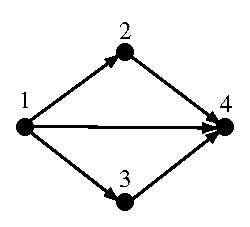
\includegraphics[scale=0.5]{graph1}
\end{center}
%
One way to represent a graph is with a dictionary \hbox{\lstinline/(vertex, vertex list) dictionary/} where
each entry in the dictionary lists the outgoing edges from that vertex.
Assume the following type definitions.

\begin{ocaml}
type vertex = int
type graph = (vertex, vertex list) dictionary
\end{ocaml}
%
Write a function \hbox{\lstinline/reachable : graph -> vertex -> vertex -> bool/}, where
\hbox{\lstinline/reachable graph v1 v2/} is \hbox{\lstinline/true/} iff vertex \hbox{\lstinline/v2/} is
reachable from \hbox{\lstinline/v1/} by following edges only in the forward direction.  Your algorithm should
terminate on all inputs.

\begin{answer}\ifanswers
To ensure that the algorithm terminates, we need to keep track of which vertices have already been
visited using a set \hbox{\lstinline/visited/} of vertices that have already been visited.  The
reachability test can be performed by a depth-first-search.

\begin{ocaml}
let reachable graph v1 v2 =
   let rec search visited v =
      if v = v2 then
         true
      else if set_mem visited v then
         false
      else
         search_list (set_insert visited v) (dict_find graph v)
   and search_list visited = function
      v :: vl -> search visited v || search_list visited vl
    | [] -> false
   in
      search set_empty v1
\end{ocaml}
\fi\end{answer}
\end{exercise}

%%%%%%%%%%%%%%%%%%%%%%%%%%%%%%%%%%%%%%%%%%%%%%%%%%%%%%%%%%%%%%%%%%%%%%%%
% Comparison
%
\begin{exercise}{set-compare}
Consider the function \hbox{\lstinline/insert/} for unbalanced, ordered, binary trees in
Section~\refsection{unbalanced-btree}.  One potential problem with this implementation is that it
uses the builtin comparison \hbox{\lstinline/(<)/}.  Rewrite the definition so the it is parameterized by a
comparison function that, given two elements, returns on of three values
%
\hbox{\lstinline/type comparison = LessThan | Equal | GreaterThan/}.
%
The expression \hbox{\lstinline/insert compare x tree/} inserts an element \hbox{\lstinline/x/} into the tree
\hbox{\lstinline/tree/}.  The type is
%
\hbox{\lstinline/insert : ('a -> 'a -> comparison) -> 'a -> 'a tree -> 'a tree/}.

\begin{answer}\ifanswers
The principal change is to use pattern matching instead of the conditional.

\begin{ocaml}
let rec insert compare x = function
   Leaf -> Node (x, Leaf, Leaf)
 | Node (y, left, right) as node ->
     match compare x y with
        LessThan -> Node (y, insert compare x left, right)
      | Equal -> node
      | GreaterThan -> Node (y, left, insert compare x right)
\end{ocaml}
\fi\end{answer}
\end{exercise}

%%%%%%%%%%%%%%%%%%%%%%%%%%%%%%%%%%%%%%%%%%%%%%%%%%%%%%%%%%%%%%%%%%%%%%%%
% Heaps
%
\begin{exercise}{heap}
A \emph{heap} of integers is a data structure supporting the following operations.

\begin{itemize}
\item \lstinline!makeheap : int -> heap!: create a heap containing a single element,
\item \lstinline!insert : heap -> int -> heap!: add an element to a heap; duplicates are allowed,
\item \lstinline!findmin : heap -> int!: return the smallest element of the heap.
\item \lstinline!deletemin : heap -> heap!: return a new heap that is the same as the original, without the smallest element.
\item \lstinline!meld : heap -> heap -> heap!: join two heaps into a new heap containing the elements of both.
\end{itemize}
%
A heap can be represented as a binary tree, where for any node $a$, if $b$ is a child node of $a$,
then $\ms{label}(a) \le \ms{label}(b)$.  The order of children does not matter.  A \emph{pairing heap} is a
particular implementation where the operations are performed as follows.

\begin{itemize}
\item \lstinline!makeheap i!: produce a single-node tree with \hbox{\lstinline/i/} at the root.
\item \lstinline!insert h i = meld h (makeheap i)!.
\item \lstinline!findmin h!: return the root label.
\item \lstinline!deletemin h!: remove the root, and \hbox{\lstinline/meld/} the subtrees.
\item \lstinline!meld h1 h2!: compare the roots, and make the heap with the larger element a subtree of the other.
\end{itemize}
%
\begin{enumerate}
\item
Define a type \hbox{\lstinline/heap/} and implement the five operations.

\begin{answer}\ifanswers
\begin{ocaml}
type heap = Node of int * heap list

let makeheap i = Node (i, [])

let meld (Node (i1, c1) as h1) (Node (i2, c2) as h2) =
   if i1 < i2 then
      Node (i1, h2 :: c1)
   else
      Node (i2, h1 :: c2)

let insert h i =
   meld h (makeheap i)

let findmin (Node (i, _)) =
   i

let deletemin = function
   Node (_, []) -> raise (Invalid_argument "deletemin")
 | Node (_, [h]) -> h
 | Node (_, h :: t) ->
     let rec meld_all h = function
        x :: t -> meld_all (meld h x) t
      | [] -> h
     in
        meld_all h t
\end{ocaml}
\fi\end{answer}

\item A \emph{heap sort} is performed by inserting the elements to be sorted into a heap,
then the values are extracted from smallest to largest.  Write a function
\hbox{\lstinline/heap_sort : int list -> int list/} that performs a heap sort,
where the result is sorted from largest to smallest.

\begin{answer}\ifanswers
\begin{ocaml}
let insert_list heap = function
   i :: elements -> insert_list (insert heap i) elements
 | [] -> heap

let heap_sort = function
   [] -> []
 | i :: elements ->
     let rec loop sorted heap =
        match heap with
           Node (i, []) -> i :: sorted
         | _ -> loop (findmin heap :: sorted) (deletemin heap)
     in
        loop [] (insert_list (makeheap i) elements)
\end{ocaml}
\fi\end{answer}
\end{enumerate}
\end{exercise}

% -*-
% Local Variables:
% Mode: LaTeX
% fill-column: 100
% TeX-master: "paper"
% TeX-command-default: "LaTeX/dvips Interactive"
% End:
% -*-
% vim:tw=100:fo=tcq:

%
%
%
\labelchapter{refcells}{Reference cells and side-effects}

Most of the values we have seen so far, like tuples and lists, are \emph{immutable}.  That is, once
a value is created, it never changes.  In this chapter we introduce operations and values for
imperative programming---programming with assignment, side-effects, and mutable state.

\label{keyword::=}
\index{reference cells}
\index{ref@\lstinline/ref/}
\index{!@\lstinline/!/ deference}
\index{:=@\lstinline/:=/ assignment}
The principal tool for imperative programming in OCaml is the \emph{reference cell}, which can be
viewed as a kind of ``box.''  The box always holds a value, but the contents of the box can be
replaced by assignment.  The operations on reference cells are as follows.

\begin{ocaml}
val ref  : 'a -> 'a ref
val (:=) : 'a ref -> 'a -> unit
val (!)  : 'a ref -> 'a
\end{ocaml}
%
Reference cells are created with the expression \hbox{\lstinline/ref e/}, which takes the initial
value \hbox{\lstinline/e/} for the reference cell.  The expression \hbox{\lstinline/!r/} returns the value in the
reference cell \hbox{\lstinline/r/}, and the expression \hbox{\lstinline/r := e/} replaces the contents of the
reference cell with the value \hbox{\lstinline/e/}.

\begin{figure}[t]
\begin{center}
\begin{tabular}{c|c}
Imperative factorial in C++ & Imperative factorial in OCaml\\
\hline\hline
\begin{clisting}
int factorial(int i) {
    int j = 1;
    for(int k = 2; k <= i; k++)
        j *= k;
    return j;
}
\end{clisting}
&
{\lstset{numbers=left,numberstyle=\tiny,firstnumber=1,stepnumber=1}
\begin{ocamllisting}
let factorial i =
    let j = ref 1 in
    for k := 2 to i do
       j := !j * k
    done;
    !j
\end{ocamllisting}}
\end{tabular}
\end{center}
\caption{Imperative implementations of a factorial function.}
\label{figure:imp-fact}
\end{figure}

For illustration, two imperative implementations of a factorial function are shown in
Figure~\ref{figure:imp-fact}, one written in C++, and the other in OCaml.  The structure of the code
is similar: the variable \hbox{\lstinline/j/} is initially defined to be \hbox{\lstinline/1/} on line 2;
then \hbox{\lstinline/j/} is multiplied by each value $2, \ldots, i$ on the for-loop in lines 3 and
4 to produce the final value $j = 1 * 2 * \cdots * i = i!$.

Structurally, the programs look quite similar, but there is a key difference in regard to the
variables.  In C, the variable \hbox{\lstinline/j/} is assigned to directly.  In OCaml, variables are
always immutable.  Instead, the variable \hbox{\lstinline/j/} refers to a reference cell and it is the
contents of the reference cell that is modified.  This also means that every time the value of the
cell is needed, the expression \hbox{\lstinline/!j/} is used.

\index{;!sequencing}
\label{keyword:;(sequencing)}
The figure also shows examples of sequencing and looping.  In OCaml, semicolons are used as
separators to specify sequencing of evaluation \hbox{\lstinline/$\nt{expression}_1$; $\nt{expression}_2$/}.
To evaluate the sequence, expression $\nt{expression}_1$ is first evaluated, the value discarded,
then the expression $\nt{expression}_2$ is evaluated and the value returned as the result of the
sequence.  It should be emphasized that the semicolon \hbox{\lstinline/;/} is not a terminator, like
it is in C.  For example, if line 6 of the OCaml factorial were followed by a semicolon, it would
mean that the value of the expression \hbox{\lstinline/!j/} should be discarded---and the value of the
function is defined by whatever follows the semicolon.

\index{loops}
\index{for-loop}
\index{while-loop}
\label{keyword:while}
\label{keyword:for}
\label{keyword:do}
\label{keyword:done}
\label{keyword:to}
\label{keyword:downto}
For-loops and while-loops are specified in one of the following forms.

\begin{ocaml}
for $\nt{identifier} := \nt{expression}_1$ to $\nt{expression}_2$ do $\nt{expression}_3$ done
for $\nt{identifier} := \nt{expression}_1$ downto $\nt{expression}_2$ do $\nt{expression}_3$ done
while $\nt{expression}_1$ do $\nt{expression}_2$ done
\end{ocaml}
%
In a for-loop, the body $\nt{expression}_3$ of the loop is evaluated for each value of the identifier
$\nt{identifier}$ between $\nt{expression}_1$ and $\nt{expression}_2$ inclusive; the \hbox{\lstinline/to/}
form counts upward by 1, and \hbox{\lstinline/downto/} counts down.  The expressions $\nt{expression}_1$
and $\nt{expression}_2$ are evaluated once, before the loop is entered.

A while-loop is evaluated by first evaluating the Boolean
expression $\nt{expression}_1$; if true, then the expression $\nt{expression}_2$ is evaluated for
its side-effect.  The evaluation is repeated until $\nt{expression}_1$ is false.  For comparison,
the factorial is implemented with a while-loop in Figure~\ref{figure:imp-fact2}.

\labelsection{pure-functional-programming}{Pure functional programming}

The one feature that is central to all functional programming languages is that functions are first
class values.  Functions can be passed as arguments and stored in data structures, just
like any other kind of value.  In fact, this is the only strict requirement for a language to be
functional, and by this definition it can be argued that many languages are functional, including C,
Javascript, OCaml, and others.

\index{pure functional programming}
A related property is \emph{purity}; a pure functional language does not include assignment or other
side-effects.  Haskell is an example of a pure functional language; OCaml and most Lisp dialects are
impure, meaning that they allow side-effects of some form.  One reason to prefer purity is that it
simplifies reasoning about programs.  In mathematics, a \emph{function} is defined as a
single-valued map, meaning that if $f$ is a function and $f(x)$ is defined for some $x$, then there
is only one value of $f(x)$.  Now, consider the following ``function'' written in C.

\begin{ccode}
int index = 1;
int g(int i) {
   index = index + 1;
   return i + index;
}
\end{ccode}
%
When called, the function modifies the variable \hbox{\lstinline/index/} by side-effect.  Mathematically
speaking, it is not a function because an expression like \hbox{\lstinline/g(0)/} can have many
possible values---in fact, the expression \hbox{\lstinline/g(0) == g(0)/} is always false!

\begin{figure}[t]
\begin{center}
\begin{tabular}{c|c}
Imperative factorial in C++ & Imperative factorial in OCaml\\
\hline\hline
\begin{clisting}
int factorial(int i) {
    int j = 1;
    while(i > 0) {
        j *= i;
        i--;
    }
    return j;
}
\end{clisting}
&
\begin{ocamllisting}
let factorial i =
    let j = ref 1 in
    let i = ref i in
    while !i > 0 do
       j := !j * !i;
       i := !i - 1
    done;
    !j
\end{ocamllisting}
\end{tabular}
\end{center}
\caption{Imperative implementations of a factorial function using while-loops.}
\label{figure:imp-fact2}
\end{figure}

\index{referential transparency}
Reasoning about imperative programs can be more difficult than it is for pure functional programs
because of the need to analyze the program state.  Pure functional programs don't have a global
mutable state, which simplifies their analysis.  More precisely, pure functional programs
provide \emph{referential transparency}, meaning that if two expressions evaluate to the same value,
then one can be substituted for the other without affecting the result of the computation.  For
example, consider an expression \hbox{\lstinline/f(0) + f(0)/}.  If the expression \hbox{\lstinline/f(0)/} is
referentially transparent, then the two occurrences can be replaced with the same value, and the
expression \hbox{\lstinline/let x = f(0) in x + x/} is equivalent (and probably more efficient).

Pure functional programming and referential transparency have many benefits.  Data structures are
persistent, meaning that once a data value is created, it cannot be changed or destroyed.  Programs
can be easier to reason about than equivalent imperative programs, and the compiler is given a great
deal of latitude in optimizations.

However, purity does have its drawbacks.  Side-effects can be useful in reducing code size.  For
example, suppose we have written a program containing a function \hbox{\lstinline/f(x)/}.  During testing,
we might want to know whether \hbox{\lstinline/f/} is ever called.  With side-effects, this is easy---we
add a flag that gets set whenever the function is called.  No other part of the program need be
changed.

\begin{ocaml}
let f_was_called = ref false

let f x =
   f_was_called := true;
   ...
\end{ocaml}
%
Without side-effects, this would be difficult to do without changing other parts of the program as
well.

Another, deeper, issue with purity is that it becomes impossible to construct some cyclic data
structures, ruling out some commonly-used data representations for graphs, circular
lists, \emph{etc}.  The problem is that, when a data value like a tuple or list is constructed, the
values it refers to must already exist.  In particular, a value being constructed may not, in
general, refer to itself.  In imperative programming, this is not an issue, because data values can be
constructed, then later mutated if a cyclic structure is desired.

A related issue is that, for some algorithms, the best known implementations are imperative.  For
these reasons, and perhaps others, OCaml supports side-effects, including operations on mutable data
and imperative input/output operations.  In the next few sections, we'll look at some common
imperative data representations using reference cells.

\labelsubsection{ref-value-restriction}{Value restriction}

\index{value restriction} As we mentioned in Section \refsection{value-restriction}, mutability and
side-effects interact with type inference.  For example, consider a ``one-shot'' function that saves
a value on its first call, and returns that value on all future calls.  This function is not
properly polymorphic because it contains a mutable field.  We illustrate this with a mutable
variable \hbox{\lstinline/x/}.

\begin{ocaml}
# let x = ref None;;
@
\begin{topoutput}
val x : '_a option ref = {contents=None}
\end{topoutput}
@
# let one_shot y =
     match !x with
        None ->
           x := Some y;
           y
      | Some z ->
           z;;
@
\begin{topoutput}
val one_shot : '_a -> '_a = <fun>
\end{topoutput}
@
# one_shot 1;;
@
\begin{topoutput}
- : int = 1
\end{topoutput}
@
# one_shot;;
@
\begin{topoutput}
val one_shot : int -> int = <fun>
\end{topoutput}
@
# one_shot 2;;
@
\begin{topoutput}
- : int = 1
\end{topoutput}
@
# one_shot "Hello";;
@
\begin{topoutput}
Characters 9-16:
This expression has type string but is here used with type int
\end{topoutput}
@
\end{ocaml}
%
The value restriction requires that polymorphism be restricted to
immutable values.  Values include functions, constants, constructors with fields
that are values, and other fully-evaluated immutable expressions.  A
function application is \emph{not} a value, and a mutable reference cell
is not a value.  By this definition, the \hbox{\lstinline/x/} and
\hbox{\lstinline/one_shot/} variables cannot be polymorphic, as the type constants
\hbox{\lstinline/'_a/} indicate.

\labelsection{queues}{Queues}

\index{queue!imperative}
A simple imperative \emph{queue} is a data structure supporting three operations.

\begin{ocaml}
val create : unit -> 'a queue
val add    : 'a queue -> 'a -> unit
val take   : 'a queue -> 'a
\end{ocaml}
%
\index{FIFO|see{queue}}
In a first-in-first-out (FIFO) queue, the queue contains a sequence of elements, and the
first element added to the queue is the first one taken out.

One way to represent a queue would be with a list, but this would mean that one of the
operations \hbox{\lstinline/add/} or \hbox{\lstinline/take/} would be required to scan to the end of the list.  An
alternative commonly used implementation is to represent the queue with two lists
$(\ms{front}, \ms{back})$ where elements are added to the list $\ms{front}$, taken from the list
$\ms{back}$, and the entire sequence of elements is
%
\hbox{\lstinline/$\ms{front}$ @ (List.rev $\ms{back}$)/}---that is,
the list $\ms{back}$ is represented in reverse order.  The first two queue functions can be
implemented as follows.

\begin{ocaml}
type 'a queue = ('a list * 'a list) ref

let create () =
   ref ([], [])

let add queue x =
   let (front, back) = !queue in
   queue := (x :: front, back)
\end{ocaml}
%
In the empty queue, both $\ms{front}$ and $\ms{back}$ are empty; the function \hbox{\lstinline/add/} simply
adds the element to $\ms{front}$ and sets the queue reference to the new value.

The function \hbox{\lstinline/take/} is only a little more complicated.  By default, values are taken from
the list $\ms{back}$.  If the list $\ms{back}$ is empty, the elements in $\ms{front}$ are
``shifted'' to $\ms{back}$ by reversing the list.

\begin{ocaml}
let rec take queue =
   match !queue with
      (front, x :: back) ->
          queue := (front, back);
          x
    | ([], []) ->
          raise (Invalid_argument "queue is empty")
    | (front, []) ->
          queue := ([], List.rev front);
          take queue
\end{ocaml}
%
Note the recursive call to \hbox{\lstinline/take/} in the final clause, which restarts the operation once
the elements have been shifted.  The worst-case complexity of the function \hbox{\lstinline/take/} is
$O(n)$ where $n$ is the number of elements in the queue.  However, if we consider the amortized
cost, ``charging'' the one extra unit of time to each \hbox{\lstinline/add/} call to account for the
list reversal, then all operations take constant $O(1)$ amortized time.

\labelsection{doubly-linked-lists}{Doubly-linked lists}

\index{lists!doubly-linked}
In the builtin type \hbox{\lstinline/'a list/}, a list element contains a value of type \hbox{\lstinline/'a/} and
a link to the next element of the list.  This means that list traversal is always ordered front-to-back.

A doubly-linked list supports efficient traversal in both directions by adding a additional link, as
shown in Figure~\ref{figure:dllist1}.  In addition to a link to the next element, each element also
has a link to the previous element.  This is a cyclic data structure, so it will necessarily be
imperative.

\begin{figure}
\centerline{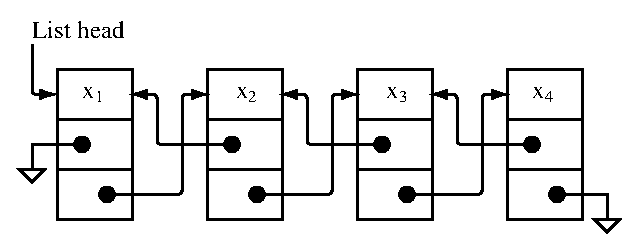
\includegraphics{dllist1}}
\caption{Doubly-linked list.}
\label{figure:dllist1}
\end{figure}

To implement the list, we'll split the operations into two parts: operations on list elements, and
operations on lists.  Given a list element, there are operations to get the next and previous
elements; and there are operations for inserting and removing elements from a list.

\begin{ocaml}
(* The type of elements in the list *)
type 'a elem

val nil_elem    : 'a elem
val create_elem : 'a -> 'a elem
val get         : 'a elem -> 'a
val prev_elem   : 'a elem -> 'a elem
val next_elem   : 'a elem -> 'a elem

(* The type of lists with elements of type 'a element *)
type 'a dllist

val create : unit -> 'a dllist
val insert : 'a dllist -> 'a elem -> unit
val remove : 'a dllist -> 'a elem -> unit
\end{ocaml}
%
The implementation starts with the list elements.  A link to an element can be null (at the end of
the list), or it can point to a real element.  Instead of having two kinds of links, we can fold the
two cases directly into the element type.  The list is designed to be modified in place, so the
links should be references to elements.

\begin{ocaml}
type 'a elem =
   Nil
 | Elem of 'a * 'a elem ref * 'a elem ref
\end{ocaml}
%
With this type definition in place, the implementation of elements is fairly straightforward.  A
fragment is shown below; the omitted functions are similar.

\begin{ocaml}
let nil_elem = Nil
let create_elem x = Elem (x, ref Nil, ref Nil)

let get = function
   Elem (x, _, _) -> x
 | Nil -> raise (Invalid_argument "get")

let prev_elem = function
   Elem (_, prev, _) -> !prev
 | Nil -> raise (Invalid_argument "prev_elem")
\end{ocaml}
%
Next, to implement the doubly-linked list, the list itself can be just be a reference to the first
element.  The function \hbox{\lstinline/create/} constructs an empty list, and \hbox{\lstinline/insert/} adds an
element at the head of the list.  The list operations are similar to what we would see on other
imperative languages; the links are modified in place as the list is changed.

\begin{ocaml}
type 'a dllist = 'a elem ref

let create () = ref Nil

let insert list elem =
   match elem, !list with
      Elem (_, prev, next), Nil ->
         prev := Nil;
         next := Nil;
         list := elem
    | Elem (_, prev1, next1), (Elem (_, prev2, _) as head) ->
         prev1 := Nil;
         next1 := head;
         prev2 := elem;
         list := elem
    | Nil, _ ->
         raise (Invalid_argument "insert")
\end{ocaml}
%
In the first case, the new element is added to an empty list; so both pointers are set
to \hbox{\lstinline/Nil/}.  In the second case, the list has a head element, which is modified so that its
previous link is now the new element.

Removing an element from the list is similar.  If the element to be removed is the head element,
then its previous link is \hbox{\lstinline/Nil/}, and the list must be updated to refer to the next
element.  Otherwise, the forward-link of the previous element must be adjusted.  Similarly, the
back-link of the next element must be adjusted.

\begin{ocaml}
let remove list elem =
   match elem with
      Elem (_, prev, next) ->
         (match !prev with
             Elem (_, _, prev_next) -> prev_next := !next
           | Nil -> list := !next);
         (match !next with
             Elem (_, next_prev, _) -> next_prev := !prev
           | Nil -> ())
    | Nil ->
         raise (Invalid_argument "remove")
\end{ocaml}

\labelsection{memoization}{Memoization}

\index{memoization}
Sometimes references and side-effects are used to improve performance without otherwise changing the
behavior of a program.  Memoization is an example of this, where a record is made of function
applications as a kind of run-time optimization.  If a function $f$ is pure, and $f(e)$ is computed
for some argument $e$, then any future computation $f(e)$ will return the same result.  When a
function $f$ is memoized, the results of function applications are stored in a table, and the
function is called at most once for any argument.

In OCaml, we can implement this in a generic way.  For immediate purposes, we'll represent the memo
(the table) as an association list.  The memoization itself can be implemented as a single higher-order function.

\begin{ocaml}
val memo : ('a -> 'b) -> ('a -> 'b)
\end{ocaml}
%
That is, the function \hbox{\lstinline/memo/} takes a function and returns a function with the same type.
The intent is that the result should be a function that is equivalent, but perhaps faster.  The memo
can be implemented as follows.

\begin{ocamlnum}
let memo f =
   let table = ref [] in
   let rec find_or_apply entries x =
      match entries with
         (x', y) :: _ when x' = x -> y
       | _ :: entries -> find_or_apply entries x
       | [] ->
          let y = f x in
          table := (x, y) :: !table;
          y
   in
   (fun x -> find_or_apply !table x)
\end{ocamlnum}
%
The memo table is defined as a mutable table on line 2; the table is filled in with argument/result
pairs as the function is called.  Given an argument \hbox{\lstinline/x/}, the
function \hbox{\lstinline/find_or_apply/} is called to search the table.  If a previous entry is found
(line 5), the previous value is returned.  Otherwise the function is called (line 8), the result is
saved in the table (line 9) by side-effect, and the value is returned.
Let's try it on a computation of Fibonacci numbers.

\begin{ocaml}
let rec fib = function
   0 | 1 as i -> i
 | i -> fib (i - 1) + fib (i - 2)
\end{ocaml}
%
To measure it, we can use the function \hbox{\lstinline/Sys.time/} to measure the CPU time taken by the process.

\begin{ocaml}
# let time f x =
   let start = Sys.time () in
   let y = f x in
   let finish = Sys.time () in
   Printf.printf "Elapsed time: %f seconds\n" (finish -. start);
   y
;;
@
\begin{topoutput}
val time : ('a -> 'b) -> 'a -> 'b = <fun>
\end{topoutput}
@
# let memo_fib = memo fib;;
@
\begin{topoutput}
val memo_fib : int -> int = <fun>
\end{topoutput}
@
# time memo_fib 40;;
@
\begin{topoutput}
Elapsed time: 14.581937 seconds
- : int = 102334155
\end{topoutput}
@
# time memo_fib 40;;
@
\begin{topoutput}
Elapsed time: 0.000009 seconds
- : int = 102334155
\end{topoutput}
@
\end{ocaml}
%
In the the first call, the computation of \hbox{\lstinline/fib 40/} took roughly 15 seconds, while the second
call was nearly instantaneous.

It should be noted that, although this kind of memoization does make use of side-effects, it has no
effect on results of the computation (as long as it is applied to pure functions).  In fact, if a
function $f$ is referentially transparent, so is \hbox{\lstinline/memo $f$/}---it behaves
as the original function, except that it trades space for time.

\labelsection{directed-graphs}{Graphs}

\index{graphs}
\index{minimum spanning tree}
\index{Kruskal's algorithm}
Let's finish this chapter with a classic algorithm from graph theory: Kruskal's algorithm for
minimum spanning trees.  Given a connected, undirected graph, a \emph{spanning tree} is a subset of
edges that forms a tree and includes every vertex.  If edges are assigned weights, the minimum
spanning tree is the spanning tree with the lowest weight.  The computation of minimum spanning
trees has many practical purposes.  One of the original uses was by Czech scientist Oscar
\misspelled{Bor\accent23{u}vka} in 1923 to minimize the cost of electrical coverage in Bohemia.

Kruskal's algorithm is specified as follows, for a weighted graph $(V, E)$ with vertices $V$ and
edges $E$.

\begin{enumerate}
\item Sort the edges $E$ by weight.
\item
For each edge in order of increasing weight, include the edge in the spanning tree if it would not form
a cycle with the edges already in the tree, otherwise discard it.
\end{enumerate}
%
The interesting part of the algorithm is step 2.  An example is shown in Figure~\ref{figure:kruskal}
for a small graph.  First, the two edges with weight 5 are added to the spanning tree.  Next, the
edges with weights 6 and 7 are added, but the edge with weight 8 is discarded because it would
produce a cycle.  Similarly, the edge with weight 9 is included, but the edge with weight 11 is
discarded, and the final edge 23 is discarded as well.

\begin{figure}
\centerline{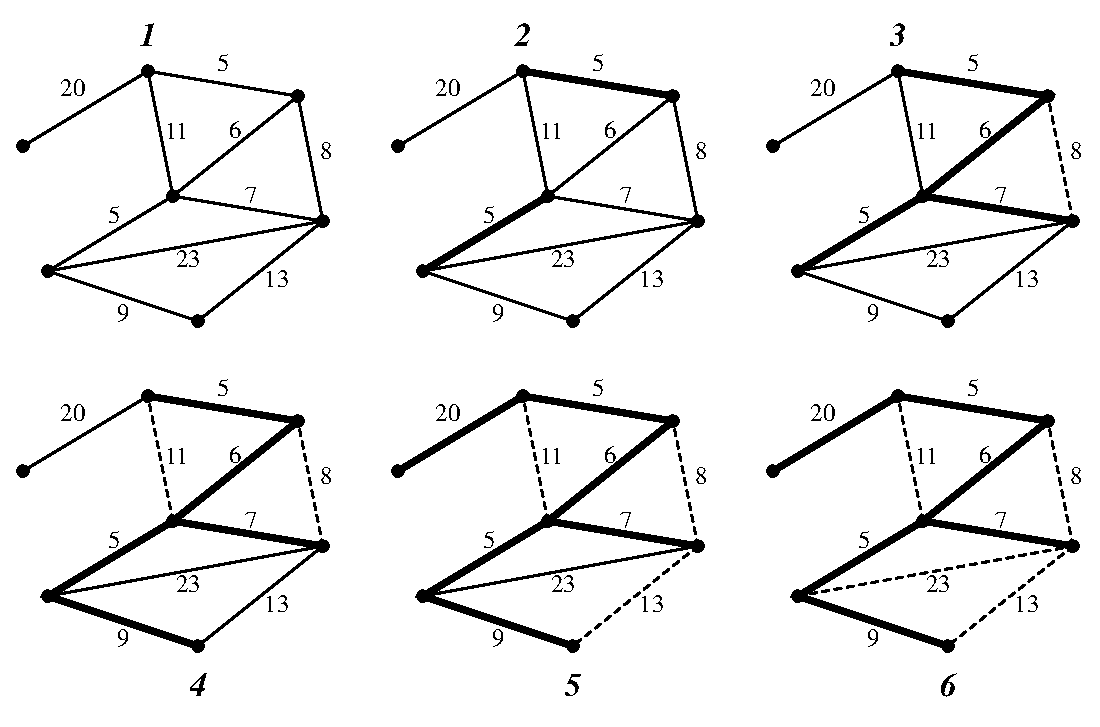
\includegraphics[scale=0.6]{kruskal}}
\caption{An example run of Kruskal's algorithm for computing the minimum spanning tree of a weighted undirected graph.}
\label{figure:kruskal}
\end{figure}

We can think of the algorithm as working over connected components of the graph.  When an edge
$(v_1, v_2)$ is included in the tree, the connected component containing $v_1$ is merged with the
component containing $v_2$.  In order to be included in the spanning tree, the vertices $v_1$ and
$v_2$ must belong to separate components---otherwise the edge would form a cycle.

We can implement this with a \emph{union-find} data structure, which supports two operations.

\begin{itemize}
\item
\lstinline/find : vertex -> vertex/,
where \hbox{\lstinline/find $v$/} returns a canonical vertex of the set (connected component) containing
$v$.  Two vertices $v_1$ and $v_2$ are in the same component if \hbox{\lstinline/find $v_1$ = find $v_2$/}.
\item
\lstinline/union : vertex -> vertex -> unit/,
where \hbox{\lstinline/union $u_1$ $u_2$/} takes the union of the sets containing canonical elements $u_1$ and $u_2$ (by side-effect).
\end{itemize}
%
Step 2 of Kruskal's algorithm can be written as follows, where the expression
%
\hbox{\lstinline/List.iter f edges/} calls the function \hbox{\lstinline/f/} for each edge in the list of edges.

\begin{ocaml}
(* An edge is a triple (weight, vertex1, vertex2) *)
type 'a edge = float * 'a vertex * 'a vertex

(* A list of edges, sorted by increasing weight *)
let kruskal edges =
   let spanning_tree = ref [] in
   List.iter (fun ((_, v1, v2) as edge) ->
      let u1 = find v1 in
      let u2 = find v2 in
      if u1 != u2 then begin
         (* v1 and v2 belong to different components *)
         spanning_tree := edge :: !spanning_tree;
         union u1 u2
      end) edges;
   !spanning_tree
\end{ocaml}
%
What remains is to specify the type for vertices, and to implement the functions \hbox{\lstinline/find/}
and \hbox{\lstinline/union/}.  One simple way to do so is to organize the vertices in each connected
component into a tree, where each vertex has a pointer to its parent.  The root of the tree is the
canonical element returned by the function \hbox{\lstinline/find/}.  Given roots \hbox{\lstinline/u1/}
and \hbox{\lstinline/u2/}, the union operation simply makes one a child of the other.
For efficiency, we use the following heuristics.

\begin{itemize}
\item When performing a \hbox{\lstinline/union/}, the smaller tree should become a child of the larger.
We'll save the size of the tree at the root.
\item
When performing a \hbox{\lstinline/find $v$/}, first find the root $u$, then traverse the path from $v$ to
$u$ a second time, updating all parent pointers to point to $u$.
\end{itemize}
%
Both heuristics will tend to make the tree fatter.  The second, called \emph{path compression},
decreases the cost of subsequent \hbox{\lstinline/find/} operations.

We'll represent a vertex as a pair \hbox{\lstinline/($\ms{label}$, $\ms{parent}$)/} where $\ms{label}$ is
the label of the vertex, and $\ms{parent}$ is the parent link: either \hbox{\lstinline/Root i/} for the
root vertex, or \hbox{\lstinline/Parent p/} if not.  The \hbox{\lstinline/union/} operation can be written as
follows.

\begin{ocaml}
type 'a parent =
   Root of int
 | Parent of 'a vertex

and 'a vertex = 'a * 'a parent ref

let union ((_, p1) as u1) ((_, p2) as u2) =
   match !p1, !p2 with
      Root size1, Root size2 when size1 > size2 ->
         p2 := Parent u1;
         p1 := Root (size1 + size2)
    | Root size1, Root size2 ->
         p1 := Parent u2;
         p2 := Root (size1 + size2)
    | _ ->
         raise (Invalid_argument "union: not roots")
\end{ocaml}
%
The \hbox{\lstinline/find/} operation is implemented in two parts: the actual find operation \hbox{\lstinline/simple_find/}, and the path compression \hbox{\lstinline/compress/}.

\begin{ocaml}
let rec compress root (_, p) =
   match !p with
      Root _ -> ()
    | Parent v -> p := Parent root; compress root v

let rec simple_find ((_, p) as v) =
   match !p with
      Root _ -> v
    | Parent v -> simple_find v

let find v =
   let root = simple_find v in
   compress root v;
   root
\end{ocaml}
%
It can be shown that with these heuristics, the complexity of step 2 of Kruskal's algorithm is $O((n
+ m) \alpha(n))$ where $n$ is the number of vertices $n = |V|$, $m$ is the number of edges $m =
|E|$, and $\alpha(n)$ is the inverse of Ackermann's function.  For any practical $n$, $\alpha(n)$ is
at most $4$, so Kruskal's algorithm effectively takes linear time.

The complexity argument is fairly long (see Kozen~\cite{Koz91} for a good explanation), but the key
benefit comes from path compression.  Suppose path compression were not used.  The first heuristic
would still ensure that path lengths are at most $\log n$ because the tree at least doubles in size
along each edge in the path from a vertex to the root of the tree, leading to a time complexity of
$O((n + m) \log n)$.  However, when path compression is used, the result of each \hbox{\lstinline/find/}
operation is effectively memoized, and the practical cost of the \hbox{\lstinline/find/} operation becomes
constant.

The principal motivation behind this example is to show that, in some cases, imperative programming
can be both simple and efficient.  While it is always possible to recode these algorithms in a pure
functional language, it is not always natural, and equivalent performance may not be achievable.

% -*-
% Local Variables:
% Mode: LaTeX
% fill-column: 100
% TeX-master: "paper"
% TeX-command-default: "LaTeX/dvips Interactive"
% End:
% -*-
% vim:tw=100:fo=tcq:

%
%
%
\exercises

%%%%%%%%%%%%%%%%%%%%%%%%%%%%%%%%%%%%%%%%%%%%%%%%%%%%%%%%%%%%%%%%%%%%%%%%
% Reference cells.
%
\begin{exercise}{ref1}
What is the value of the following expressions?

\begin{enumerate}
\item \lstinline|let x = ref 1 in let y = x in y := 2; !x|

\begin{answer}\ifanswers
The variables \hbox{\lstinline/x/} and \hbox{\lstinline/y/} refer to the same reference cell, so the result is \hbox{\lstinline/2/}.
\fi\end{answer}

\item \lstinline|let x = ref 1 in let y = ref 1 in y := 2|

\begin{answer}\ifanswers
The variables \hbox{\lstinline/x/} and \hbox{\lstinline/y/} refer to different reference cells, so the result is \hbox{\lstinline/1/}.
\fi\end{answer}

\item

\begin{ocamllisting}
let x = ref 1 in
let y = ref x in
!y := 2;
!x
\end{ocamllisting}

\begin{answer}\ifanswers
Since \hbox{\lstinline/y/} refers to \hbox{\lstinline/x/}, assigning to \hbox{\lstinline/!y/} is the same as assigning to \hbox{\lstinline/x/}.
The final value \hbox{\lstinline/!x/} is \hbox{\lstinline/2/}.
\fi\end{answer}

\item

\begin{ocamllisting}
let fst (x, _) = x in
let snd (_, x) = x in
let y = ref 1 in
let x = (y, y) in
fst x := 2;
!(snd x)
\end{ocamllisting}

\begin{answer}\ifanswers
Both elements of the pair \hbox{\lstinline/(y, y)/} refer to the same cell, so the assignment \hbox{\lstinline/fst x := 2/}
effects both parts; the value \hbox{\lstinline/!(snd x)/} is \hbox{\lstinline/2/}.
\fi\end{answer}

\item

\begin{ocamllisting}
let x = ref 0 in
let y = ref [5; 7; 2; 6] in
while !y <> [] do
   x := !x + 1;
   y := List.tl !y
done;
!x
\end{ocamllisting}

\begin{answer}\ifanswers
The variable \hbox{\lstinline/x/} is incremented for each element of the list \hbox{\lstinline/y/}, so the final
value \hbox{\lstinline/!x/} is \hbox{\lstinline/4/}.
\fi\end{answer}

\end{enumerate}
\end{exercise}

%%%%%%%%%%%%%%%%%%%%%%%%%%%%%%%%%%%%%%%%%%%%%%%%%%%%%%%%%%%%%%%%%%%%%%%%
% Lazy values
%
\begin{exercise}{lazy}
\label{keyword:lazy}
\index{lazy value}
A \emph{lazy} value is a computation that is deferred until it is needed; we say that it is
\emph{forced}.  A forced value is memoized, so that subsequent forcings do not reevaluate the
computation.  The OCaml standard library already provides an implementation of lazy values in the
\hbox{\lstinline/Lazy/} module, but we can also construct them ourselves using reference cells and
functions.

\begin{ocaml}
type 'a deferred
val defer : (unit -> 'a) -> 'a deferred
val force : 'a deferred -> 'a
\end{ocaml}
%
Implement the type \hbox{\lstinline/'a deferred/} and the functions \hbox{\lstinline/defer/} and \hbox{\lstinline/force/}.

\begin{answer}\ifanswers
The important part is that the forcing is memoized.  We can use a reference cell to save to computation.

\begin{ocaml}
type 'a deferred_value =
   Deferred of (unit -> 'a)
 | Forced of 'a

type 'a deferred = 'a deferred_value ref

let defer f = ref (Deferred f)

let force cell =
   match !cell with
      Deferred f ->
         let result = f () in
         cell := Forced result;
         result
    | Forced result ->
         result
\end{ocaml}
\fi\end{answer}
\end{exercise}

%%%%%%%%%%%%%%%%%%%%%%%%%%%%%%%%%%%%%%%%%%%%%%%%%%%%%%%%%%%%%%%%%%%%%%%%
% Lazy lists
%
\begin{exercise}{lazy-list}
\index{lazy list}
A lazy list is a list where the tail of the list is a deferred computation (a lazy list is also
called a \emph{stream}).  The type can be defined as follows, where the type \hbox{\lstinline/deferred/} is
defined as in Exercise~\ref{exercise:lazy}.

\begin{ocaml}
type 'a lazy_list =
   Nil
 | Cons of 'a * 'a lazy_list
 | LazyCons of 'a * 'a lazy_list deferred
\end{ocaml}
%
Define the following functions on lazy lists.

\begin{ocamlx}
val nil       : 'a lazy_list
val cons      : 'a -> 'a lazy_list -> 'a lazy_list
val lazy_cons : 'a -> (unit -> 'a lazy_list) -> 'a lazy_list
val is_nil    : 'a lazy_list -> bool
val head      : 'a lazy_list -> 'a
val tail      : 'a lazy_list -> 'a lazy_list
val (@@)      : 'a lazy_list -> 'a lazy_list -> 'a lazy_list
\end{ocamlx}
%
The expression \hbox{\lstinline/$l_1$ @@ $l_2$/} appends two lazy lists in constant time.

\begin{answer}\ifanswers
The implementations are as follows.

\begin{ocamlx}
let nil = Nil
let cons h t = Cons (h, t)
let lazy_cons h f = LazyCons (h, defer f)

let is_nil = function
   Nil -> true
 | Cons _ | LazyCons _ -> false

let head = function
   Nil -> raise (Invalid_argument "head")
 | Cons (h, _)
 | LazyCons (h, _) -> h

let tail = function
   Nil -> raise (Invalid_argument "tail")
 | Cons (_, t) -> t
 | LazyCons (_, f) -> force f

let rec (@@) l1 l2 =
   match l1, l2 with
      Nil, l | l, Nil -> l
    | _ -> lazy_cons (head l1) (fun () -> tail l1 @@ l2)
\end{ocamlx}
\fi\end{answer}
\end{exercise}

%%%%%%%%%%%%%%%%%%%%%%%%%%%%%%%%%%%%%%%%%%%%%%%%%%%%%%%%%%%%%%%%%%%%%%%%
% Queues.
%
\begin{exercise}{fun-queue}
\index{queue!functional}
The FIFO queues described in Section~\ref{section:queues} are imperative; whenever a value is added to
or taken from the queue, the queue is modified by side-effect.  Implement a \emph{persistent} queue
with the following operations.

\begin{ocaml}
val empty : 'a queue
val add   : 'a queue -> 'a -> 'a queue
val take  : 'a queue -> 'a * 'a queue
\end{ocaml}
%
The expression \hbox{\lstinline/add queue e/} produces a new queue, without affecting the contents of the
original queue \hbox{\lstinline/queue/}.  The expression \hbox{\lstinline/take queue/} returns an element of the
queue \hbox{\lstinline/queue/} and a new queue; again, the contents of the original queue \hbox{\lstinline/queue/}
are unaffected.

$\star$ Can you implement the queue so that any sequence of $n$ \hbox{\lstinline/add/} and \hbox{\lstinline/take/}
operations, in any order, take $O(n)$ time?  Hint: consider using lazy lists
(Exercise~\ref{exercise:lazy-list}) to represent the queue, shifting the queue whenever the
$\ms{front}$ is longer than the $\ms{back}$.  See Okasaki~\cite{Oka95}.

\begin{answer}\ifanswers
The queue could simply be represented as a list, but then one of the operations \hbox{\lstinline/add/} or
\hbox{\lstinline/take/} would take time $O(m)$ where $m$ is the length of the queue.

The two list \hbox{\lstinline/($\ms{front}$, $\ms{back}$)/} representation is a little better.  To make the
data structure persistent, the functions \hbox{\lstinline/add/} and \hbox{\lstinline/take/} produce new queues.

\begin{ocamlnum}
type 'a queue = ('a list * 'a list) ref

let empty = ref ([], [])

let add queue x =
   let (front, back) = !queue in
   ref (x :: front, back)

let rec take queue =
   match !queue with
      [], [] -> raise (Invalid_argument "queue")
    | front, x :: back ->
        x, ref (front, back)
    | front, [] ->
        queue := ([], List.rev front);
        take queue
\end{ocamlnum}
%
The side effect on line 15 does not affect persistence because the queue membership is preserved.
However, efficiency is still not optimal.  Consider a sequence of $m$ \hbox{\lstinline/add/}s, followed by $m$ \hbox{\lstinline/take/}s.

\begin{ocaml}
let $q_1$ = add empty 1
let $q_2$ = add $q_1$ 2
...
let $q_m$ = add $q_{m - 1}$ $m$
let $x_m$, _ = take $q_m$
let $x_{m - 1}$, _ = take $q_{m - 1}$
...
let $x_1$, _ = take $q_1$
\end{ocaml}
%
Each operation \hbox{\lstinline/take $q_i$/} shifts $i$ elements of the queue, so the total time is $O(m^2)$.

Okasaki gives an efficient implementation, summarized below in OCaml.  A function
\hbox{\lstinline/maybe_shift/} is used to shift the queue whenever the front becomes longer than the back.
The list lengths are needed, so the queue is a 4-tuple
%
\hbox{\lstinline/($\ms{front}$, $|\ms{front}|$, $\ms{back}$, $|\ms{back}|$)/}.

\begin{ocaml}
type 'a queue = 'a lazy_list * int * 'a lazy_list * int

let empty = (Nil, 0, Nil, 0)

let insert (front, flen, back, blen) x =
   maybe_shift (cons x front) (flen + 1) back blen

let remove (front, flen, back, blen) =
   head back, maybe_shift front flen (tail back) (blen - 1)

let maybe_shift front flen back blen =
   if flen <= blen then
      (front, flen, back, blen)
   else
      (Nil, 0, shift front back [], flen + blen)

let shift front back l =
   if is_nil back then
      cons (head front) l
   else
      lazy_cons (head back) (fun () ->
         shift (tail front) (tail back) (cons (head front) l))
\end{ocaml}
\fi\end{answer}
\end{exercise}

%%%%%%%%%%%%%%%%%%%%%%%%%%%%%%%%%%%%%%%%%%%%%%%%%%%%%%%%%%%%%%%%%%%%%%%%
% Memoization
%
\begin{exercise}{memoization}
\index{memoization!of recursive functions}
One problem with the memoization function \hbox{\lstinline/memo : ('a -> 'b) -> ('a -> 'b)/} in
Section~\ref{section:memoization} is that it ignores recursive definitions.  For example,
the expression \hbox{\lstinline/memo fib $i$/} still takes exponential time in $i$ to compute.

To solve this, we'll need to modify the recursive definition for \hbox{\lstinline/fib/} and perform an
explicit memoization.  Implement the following types and functions, where
%
\hbox{\lstinline/fib = memo_fib (create_memo ())/}.  How fast is the Fibonacci function now?

\begin{ocaml}
type ('a, 'b) memo
val create_memo : unit -> ('a, 'b) memo
val memo_find   : ('a, 'b) memo -> 'a -> 'b option
val memo_add    : ('a, 'b) memo -> 'a -> 'b -> unit
val memo_fib    : (int, int) memo -> int -> int

let fib = memo_fib (create_memo ())
\end{ocaml}

\begin{answer}\ifanswers
The main task here is to separate the parts of the memoization.  We'll use a simple association list
for the memo table.  The expression \hbox{\lstinline/fib $n$/} is computed in quadratic time $O(n^2)$.  A
more efficient implementation of the dictionary would reduct this to no more than $O(n \log n)$
time.

\begin{ocaml}
type ('a, 'b) memo = ('a * 'b) list

let create_memo () = []

let rec memo_find table x =
   match table with
      (x', y) :: _ when x' = x -> Some y
    | _ :: table -> memo_find table x
    | [] -> None

let memo_fib table i =
   match memo_find table i with
      Some j -> j
    | None -> 
        match i with
           0 | 1 -> i
         | _ ->
            let j = memo_fib table (i - 1) + memo_fib table (i - 2) in
            memo_add table i j;
            j
\end{ocaml}
\fi\end{answer}
\end{exercise}

%%%%%%%%%%%%%%%%%%%%%%%%%%%%%%%%%%%%%%%%%%%%%%%%%%%%%%%%%%%%%%%%%%%%%%%%
% Directed graphs
%
\begin{exercise}{dfs}
\index{depth-first search}
One way to represent a directed graph is with an adjacency list stored directly in each vertex.
Each vertex has a label and a list of out-edges; we also include a ``mark'' flag and an integer to
be used by a depth-first-search.

\begin{ocaml}
type 'a vertex =
   (* Vertex (label, out-edges, dfs-mark, dfs-index) *)
   Vertex of 'a * 'a vertex list ref * bool ref * int option ref

type 'a directed_graph = 'a vertex list
\end{ocaml}
%
Depth-first search and breadth-first search are two highly useful graph algorithms.
A depth-first search (DFS) traverses the graph, assigning to each vertex a DFS index and
marking a vertex $v$ when all out-edges of $v$ have been explored.  The DFS search is performed as follows.

Choose an unmarked vertex $u$ in the graph, push out-edges $(u, v)$ onto a stack.  Assign $u$ DFS index 0, set
the DFS counter $c$ to 1, and then repeat the following until the stack is empty.

\begin{enumerate}
\item Pop an edge $(u, v)$ from the stack, and classify it according to the following
table.

\begin{center}
\begin{tabular}{l|l}
Condition & Edge type for $(u, v)$\\
\hline
$v$ does not have a DFS index & tree edge\\
$\ms{DFS}(u) < \ms{DFS}(v)$ & forward edge\\
$\ms{DFS}(u) > \ms{DFS}(v)$ and $v$ not marked & back edge\\
$\ms{DFS}(u) > \ms{DFS}(v)$ and $v$ marked & cross edge
\end{tabular}
\end{center}
%
\item
If $(u, v)$ is a tree edge, assign $v$ the current DFS index $c$, increment $c$, and push all edges
$(v, w)$ onto the stack.
\item
When all edges $(u, v)$ have been considered, mark the vertex $u$.
\end{enumerate}
%
Repeat until all vertices have been marked.
A graph is \emph{cyclic} iff the DFS search found any back-edges.

Implement a DFS search.  You can assume that all vertices are initially unmarked and their DFS index
is \hbox{\lstinline/None/}.

\begin{answer}\ifanswers
We'll keep a flag \hbox{\lstinline/cyclic/} to indicate whether the graph is cyclic.  First, all the mark
bits and DFS counters are cleared, then the function \hbox{\lstinline/search/} is called to perform the DFS
search.  It isn't necessary to keep an explicit stack of edges---in effect, the OCaml runtime stack
is serving as the edge stack.

\begin{ocaml}
let rec dfs graph =
   let cyclic = ref false in
   let dfs_counter = ref 0 in

   (* The main DFS search *)
   let rec search (Vertex (_, u_edges, u_mark, u_index)) =
      if not !u_mark then begin
         let c = !dfs_counter in
         u_index := Some c;
         dfs_counter := c + 1;
         List.iter (fun (Vertex (_, _, v_mark, v_index) as v) ->
            match !v_index with
               Some index ->
                  if index < c && not !v_mark then
                     cyclic := true
             | None ->
                  search v) !u_edges;
         u_mark := true
      end
   in

   (* Reset the graph state *)
   List.iter (fun (Vertex (_, _, mark, index)) ->
      mark := false;
      index := None) graph;

   (* DFS over all the vertices in the graph *)
   List.iter search graph
\end{ocaml}
\fi\end{answer}
\end{exercise}

%%%%%%%%%%%%%%%%%%%%%%%%%%%%%%%%%%%%%%%%%%%%%%%%%%%%%%%%%%%%%%%%%%%%%%%%
% Copying
%
\begin{exercise}{graph-map}
One issue with graph data structures is that some familiar operations are hard to implement.  For
example, consider the following representation (similar to the previous exercise) for a directed graph.

\begin{ocaml}
(* Vertex (label, out-edges) *)
type 'a vertex = Vertex of 'a * 'a vertex list ref
type 'a directed_graph = 'a vertex list
\end{ocaml}
%
Suppose we want to define a polymorphic map function on graphs.

\begin{ocaml}
val graph_map : ('a -> 'b) -> 'a directed_graph -> 'b directed_graph
\end{ocaml}
%
Given an arbitrary function \hbox{\lstinline/f : 'a -> 'b/} and a graph \hbox{\lstinline/g/}, the expression
\hbox{\lstinline/graph_map f g/} should produce a graph isomorphic to \hbox{\lstinline/g/}, but where
\hbox{\lstinline/f/} has been applied to each label.  Is the function \hbox{\lstinline/graph_map/} definable?  If
so, describe the implementation.  If not, explain why not.  Is there another implementation of
graphs where \hbox{\lstinline/graph_map/} can be implemented efficiently?

\begin{answer}\ifanswers
The function \hbox{\lstinline/graph_map/} is definable, but it is difficult to implement it efficiently.
The central issue is that, in order to preserve the structure of the graph, the function
\hbox{\lstinline/graph_map/} must be memoized using physical equality.  The following code gives a simple,
but inefficient, implementation.

\begin{ocamlnum}
let graph_map f graph =
   let memo = ref [] in
   let rec map u = function
      (u', v) :: table when u' == u -> v
    | _ :: table -> map u table
    | [] ->
       let (label, out_edges) = u in
       let new_out_edges = ref [] in
       let new_u = (f label, new_out_edges) in
       memo := (u, new_u) :: !memo;
       new_out_edges := map_list !out_edges
   and map_list edges =
      List.map (fun v -> map v !memo) edges
   in
   map_list graph
\end{ocamlnum}
%
The function \hbox{\lstinline/map/} searches through the memo table in linear order, looking for an entry
that matches with physical equality (\hbox{\lstinline/==/}).  If so, the previous result is returned.
Otherwise, a new vertex is created and added to the memo table.  Note that the new vertex
\hbox{\lstinline/new_u/} is added before following the out-edges recursively, preventing infinite looping
on cyclic graphs.

Given a graph with $n$ vertices and $m$ edges, the function \hbox{\lstinline/map/} examines $n$ vertices worst case, so the total time complexity is of \hbox{\lstinline/graph_map/} is $O(nm)$.

An alternative representation that would support an efficient map is to give vertices unique names,
and refer to them by name rather than referring to them directly.  The penalty is that edge
traversal takes time $O(\log n)$ rather than constant time because of the dictionary lookup.

\begin{ocaml}
(* A name for a vertex *)
type name = int

(* A vertex is (label, out-edges) *)
type 'a vertex = 'a * name list ref

(* A graph is (vertices, vertex dictionary) *)
type 'a graph = name list * (name, 'a vertex) dictionary

let graph_map f (vertices, dict) =
   vertices, dictionary_map f dict
\end{ocaml}
\fi\end{answer}
\end{exercise}

% -*-
% Local Variables:
% Mode: LaTeX
% fill-column: 100
% TeX-master: "paper"
% TeX-command-default: "LaTeX/dvips Interactive"
% End:
% -*-
% vim:tw=100:fo=tcq:

\labelchapter{records}{Records, Arrays, and String}

Records, arrays, and strings are aggregate data types.  A record is
like a tuple where the elements of the tuple are named.  Arrays and
strings are fixed-length sequences of data supporting random access to
the elements in constant time.  All three types support mutation of
elements, by assignment.

\labelsection{sect-records}{Records}

\label{keyword:records}
\index{types!records}
\index{;!record field separator}
\index{\{\}@\lstinline/{ $\cdots$ }/ records}
\index{identifiers!record labels}
A record is a labeled collection of values of arbitrary types.  The
syntax for a record type is a set of field type definitions surrounded
by braces, and separated by semicolons.  Fields are declared as
\hbox{\lstinline/label : type/}, where the label is an identifier that must begin
with a lowercase letter or an underscore.  For example, the following
record redefines the database entry from Chapter~\refchapter{tuples}.

\begin{ocaml}
# type db_entry =
     { name   : string;
       height : float;
       phone  : string;
       salary : float
     };;
@
\begin{topoutput}
type db_entry = { name: string; height: float;
                  phone: string; salary: float }
\end{topoutput}
@
\end{ocaml}
%
The syntax for a record value is similar to the type declaration, but the
fields are defined as \hbox{\lstinline/label = expr/}.  Here is an example
database entry.

\begin{ocaml}
# let jason =
     { name   = "Jason";
       height = 6.25;
       phone  = "626-555-1212";
       salary = 50.0
     };;
@
\begin{topoutput}
val jason : db_entry =
  {name="Jason"; height=6.25;
   phone="626-555-1212"; salary=50}
\end{topoutput}
@
\end{ocaml}
%
\index{.!record projection}
\index{record projection}
\label{keyword:.}
There are two ways to access the fields in a record.  The
projection operation \hbox{\lstinline/r.l/} returns the field labeled \hbox{\lstinline/l/} in
record \hbox{\lstinline/r/}.

\begin{ocaml}
# jason.height;;
@
\begin{topoutput}
- : float = 6.25
\end{topoutput}
@
# jason.phone;;
@
\begin{topoutput}
- : string = "626-555-1212"
\end{topoutput}
@
\end{ocaml}
%
\label{patterns:record}
Pattern matching can also be used to access the fields of a record.
The syntax for a pattern is like a record value, but the fields
contain a label and a pattern \hbox{\lstinline/label = patt/}.  Not all of the
fields have to be included.  Note that the binding occurrences of the
variables \hbox{\lstinline/n/} and \hbox{\lstinline/h/} occur to the \emph{right} of the equality symbol
in their fields.

\begin{ocaml}
# let { name = n; height = h } = jason;;
@
\begin{topoutput}
val n : string = "Jason"
val h : float = 6.25
\end{topoutput}
@
\end{ocaml}

\labelsubsection{record-update}{Functional and imperative record updates}

\label{records:record-update}
\index{records!functional update}
\index{with@\lstinline/with/ (functional record update)}
There is a functional update operation that produces a copy of a
record with new values for the specified fields.  The syntax for
functional update uses the \hbox{\lstinline/with/} keyword in a record definition.

\begin{ocaml}
# let dave = { jason with name = "Dave"; height = 5.9 };;
@
\begin{topoutput}
val dave : db_entry =
  {name="Dave"; height=5.9; phone="626-555-1212"; salary=50}
\end{topoutput}
@
# jason;;
@
\begin{topoutput}
- : db_entry = {name="Jason"; height=6.25;
                phone="626-555-1212"; salary=50}
\end{topoutput}
@
\end{ocaml}
%
\label{keyword:mutable(records)}
\index{mutable!record fields}
Record fields can also be modified by assignment, but only if the
record field is declared as mutable in the type definition for the
record.  The syntax for a mutable field uses the \hbox{\lstinline/mutable/}
keyword before the field label.  For example, if we wanted to allow
salaries to be modified, we would need to declare the field \hbox{\lstinline/salary/}
as \hbox{\lstinline/mutable/}.

\begin{ocaml}
# type db_entry =
     { name : string;
       height : float;
       phone : string;
       mutable salary : float
     };;
@
\begin{topoutput}
type db_entry =
  { name: string;
    height: float;
    phone: string;
    mutable salary: float }
\end{topoutput}
@
# let jason =
    { name = "Jason";
      height = 6.25;
      phone = "626-555-1212";
      salary = 50.0
    };;
@
\begin{topoutput}
val jason : db_entry =
  {name="Jason"; height=6.25; phone="626-555-1212"; salary=50}
\end{topoutput}
@
\end{ocaml}
%
\label{keyword:<-(record-field-assignment)}
\index{records!field assignment}
\index{<-!record field assignment}
The syntax for a field update is \hbox{\lstinline/r.label <- expr/}.  For example,
if we want to give \hbox{\lstinline/jason/} a raise, we would use the following statement.

\begin{ocaml}
# jason.salary <- 150.0;;
@
\begin{topoutput}
- : unit = ()
\end{topoutput}
@
# jason;;
@
\begin{topoutput}
- : db_entry = {name="Jason"; height=6.25; phone="626-555-1212"; salary=150}
\end{topoutput}
@
\end{ocaml}
%
Note that the assignment statement itself returns the canonical unit
value \hbox{\lstinline/()/}.  That is, it doesn't return a useful value, unlike
the functional update.  A functional update creates a completely new
copy of a record; assignments to the copies do not interfere.

\begin{ocaml}
# let dave = { jason with name = "Dave" };;
@
\begin{topoutput}
val dave : db_entry =
  {name="Dave"; height=6.25; phone="626-555-1212"; salary=150}
\end{topoutput}
@
# dave.salary <- 180.0;;
@
\begin{topoutput}
- : unit = ()
\end{topoutput}
@
# dave;;
@
\begin{topoutput}
- : db_entry = {name="Dave"; height=6.25; phone="626-555-1212"; salary=180}
\end{topoutput}
@
# jason;;
@
\begin{topoutput}
- : db_entry = {name="Jason"; height=6.25; phone="626-555-1212"; salary=150}
\end{topoutput}
@
\end{ocaml}

\labelsubsection{record-labels}{Field label namespace}

\index{records!field namespace}
One important point: the namespace for toplevel record field labels is
flat.  This is important if you intend to declare records with the
same field names.  If you do, the original labels will be lost!  For
example, consider the following sequence.

\begin{ocaml}
# type rec1 = { name : string; height : float };;
@
\begin{topoutput}
type rec1 = { name: string; height: float }
\end{topoutput}
@
# let jason = { name = "Jason"; height = 6.25 };;
@
\begin{topoutput}
val jason : rec1 = {name="Jason"; height=6.25}
\end{topoutput}
@
# type rec2 = { name : string; phone : string };;
@
\begin{topoutput}
type rec2 = { name: string; phone: string }
\end{topoutput}
@
# let dave = { name = "Dave"; phone = "626-555-1212" };;
@
\begin{topoutput}
val dave : rec2 = {name="Dave"; phone="626-555-1212"}
\end{topoutput}
@
# jason.name;;
@
\begin{toperror}
Characters 0-5:
This expression has type rec1 but is here used with type rec2
\end{toperror}
@
# dave.name;;
@
\begin{topoutput}
- : string = "Dave"
\end{topoutput}
@
# let bob = { name = "Bob"; height = 5.75 };;
@
\begin{toperror}
Characters 10-41:
The label height belongs to the type rec1
but is here mixed with labels of type rec2
\end{toperror}
@
\end{ocaml}
%
In this case, the \hbox{\lstinline/name/} field was redefined in the
type definition for \hbox{\lstinline/rec2/}.  At this point, the
original \hbox{\lstinline/rec1.name/} label is lost, making it
impossible to access the name field in a value of type
\hbox{\lstinline/rec1/}, and impossible to construct new values of
type \hbox{\lstinline/rec1/}.  It is, however, permissible to use the
same label names in separate files, as we will see in
Chapter~\refchapter{modules}.

\labelsection{arrays}{Arrays}

\label{keyword:arrays}
\index{arrays}
\index{[ ]@\lstinline/[$\pipe \cdots \pipe$]/ arrays}
Arrays are fixed-size vectors of values.  All of the values must have
the same type.  The fields in the array can be accessed and modified
in constant time.  Arrays can be created with the syntax
%
\hbox{\lstinline/[| $e_1$; $e_2$; $\cdots$; $e_n$ |]/},
which creates an array of length $n$ initialized with
the values computed from the expressions $e_1, \ldots, e_n$.

\begin{ocaml}
# let a = [|1; 3; 5; 7|];;
@
\begin{topoutput}
val a : int array = [|1; 3; 5; 7|]
\end{topoutput}
@
\end{ocaml}
%
\label{patterns:arrays}
\label{keyword:.(}
\index{.()@\lstinline/.()/ array subscripting}
Fields can be accessed with the \hbox{\lstinline/a.(i)/} construction.  Array
indexes start from 0, and runtime checking is used to ensure that indexes are
within the array bounds.

\begin{ocaml}
# a.(0);;
@
\begin{topoutput}
- : int = 1
\end{topoutput}
@
# a.(1);;
@
\begin{topoutput}
- : int = 3
\end{topoutput}
@
# a.(5);;
@
\begin{topoutput}
Uncaught exception: Invalid_argument("Array.get")
\end{topoutput}
@
\end{ocaml}
%
\label{keyword:<-(array-field-assignment)}
\index{<-!array field assignment}
Fields are updated with the \hbox{\lstinline/a.(i) <- e/} assignment
statement.

\begin{ocaml}
# a.(2) <- 9;;
@
\begin{topoutput}
- : unit = ()
\end{topoutput}
@
# a;;
@
\begin{topoutput}
- : int array = [|1; 3; 9; 7|]
\end{topoutput}
@
\end{ocaml}
%
\index{Array module!length@\lstinline/length/}
The \hbox{\lstinline/Array/} library module defines additional functions on arrays.
Arrays of arbitrary length can be created with the \hbox{\lstinline/Array.create/}
function, which requires a length and initializer argument.  The
\hbox{\lstinline/Array.length/} function returns the number of elements in the
array.

\begin{ocaml}
# let a = Array.create 10 1;;
@
\begin{topoutput}
val a : int array = [|1; 1; 1; 1; 1; 1; 1; 1; 1; 1|]
\end{topoutput}
@
# Array.length a;;
@
\begin{topoutput}
- : int = 10
\end{topoutput}
@
\end{ocaml}
%
\index{Array module!blit@\lstinline/blit/}
The \hbox{\lstinline/Array.blit/} function can be used to copy elements
destructively from one array to another.  The \hbox{\lstinline/blit/} function
requires five arguments: the source array, a starting offset into the
array, the destination array, a starting offset into the destination
array, and the number of elements to copy.

\begin{ocaml}
# Array.blit [| 3; 4; 5; 6 |] 1 a 3 2;;
@
\begin{topoutput}
- : unit = ()
\end{topoutput}
@
# a;;
@
\begin{topoutput}
- : int array = [|1; 1; 1; 4; 5; 1; 1; 1; 1; 1|]
\end{topoutput}
@
\end{ocaml}

\labelsection{strings}{Strings}

\label{keyword:string-subscript}
\label{keyword:<-(string-assignment)}
\index{strings}
\index{.[@\lstinline/.[]/ string subscripting}
\index{<-!string assignment}
In OCaml, strings are a lot like packed arrays of characters.  The
access and update operations use the syntax \hbox{\lstinline/s.[i]/} and
\hbox{\lstinline/s.[i] <- c/}.

\begin{ocaml}
# let s = "Jason";;
@
\begin{topoutput}
val s : string = "Jason"
\end{topoutput}
@
# s.[2];;
@
\begin{topoutput}
- : char = 's'
\end{topoutput}
@
# s.[3] <- 'y';;
@
\begin{topoutput}
- : unit = ()
\end{topoutput}
@
# s;;
@
\begin{topoutput}
- : string = "Jasyn"
\end{topoutput}
@
\end{ocaml}
%
\index{String module!length@\lstinline/length/}
\index{String module!blit@\lstinline/blit/}
The \hbox{\lstinline/String/} module defines additional functions, including the
\hbox{\lstinline/String.length/} and \hbox{\lstinline/String.blit/} functions that parallel
the corresponding \hbox{\lstinline/Array/} operations.  The \hbox{\lstinline/String.create/}
function does not require an initializer.  It creates a string with
arbitrary contents.

\begin{ocaml}
# String.create 10;;
@
\begin{topoutput}
- : string = "\000\011\000\000,\200\027x\000\000"
\end{topoutput}
@
# String.create 10;;
@
\begin{topoutput}
- : string = "\196\181\027x\001\000\000\000\000\000"
\end{topoutput}
@
\end{ocaml}

\labelsection{hash-tables}{Hash tables}

To illustrate these types in action, let's implement (yet another)
dictionary, this time in the form of a hash table.  A \emph{hash
table} provides the usual map from keys to values, but this time the
expected running time for lookup and insertion is constant.  The hash table
works by computing an integer \emph{hash} of a key that serves as an
index into an array of dictionary entries.  Insertion is performed by
adding a new entry to the table at the hash index of the key; lookup
is performed by searching for an entry with a matching key at the
key's hash index.  An example of a hash table is shown in
Figure~\ref{figure:hash-table}.

\begin{figure}
\centerline{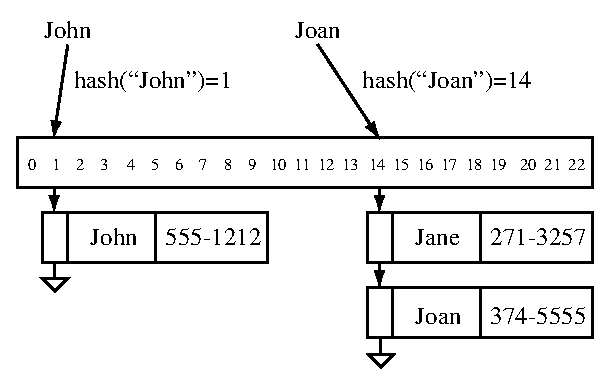
\includegraphics{hash}}
\caption{An open hash table.}
\label{figure:hash-table}
\end{figure}

In the usual case, the space of indices is smaller than the space of
keys, so hash \emph{collisions} may occur where two keys hash to the
same index.  Hash collisions can have a significant impact on
performance.  The hash table in the figure shows a so-called
``chained'' implementation, where entries with the same hash are
stored in a list associated with that index.

For our example, we'll implement a simple hash table where the keys
are strings, and the table is polymorphic over the type of values.
One approach to producing a fast, fairly good hash is called
a \emph{s-box} (for \emph{substitution box}), which uses a table of
randomly-generated numbers.

\begin{ocamlblock}
\begin{ocamlblocksize}
\begin{lstlisting}[name=hash]
let random_numbers =
   [|0x04a018c6; 0x5ba7b0f2; 0x04dcf08b; 0x1e5a22cc; 0x2523b9ea; $\cdots$|]
let random_length = Array.length random_numbers

type hash_info = { mutable hash_index : int; mutable hash_value : int }

let hash_char info c =
   let i = Char.code c in
   let index = (info.hash_index + i + 1) mod random_length in
   info.hash_value <- (info.hash_value * 3) lxor random_numbers.(index);
   info.hash_index <- index
\end{lstlisting}
\end{ocamlblocksize}
%
The record type \hbox{\lstinline/hash_info/} has two fields:
the \hbox{\lstinline/hash_index/} is an index into the random number array,
and \hbox{\lstinline/hash_value/} is the partially computed hash.  The
function \hbox{\lstinline/hash_char/} uses the character to update
the \hbox{\lstinline/hash_index/} and updates the \hbox{\lstinline/hash_value/} by
taking the exclusive-or with a random integer.  The hash of a string
is computed one character at a time.

\begin{ocamlblocksize}
\begin{lstlisting}[name=hash]
let hash s =
   let info = { hash_index = 0; hash_value = 0 } in
   for i = 0 to String.length s - 1 do
      hash_char info s.[i]
   done;
   info.hash_value
\end{lstlisting}
\end{ocamlblocksize}
%
Note that the bounds in the for-loop on line 3 are \emph{inclusive};
the index of the first character in the string is \hbox{\lstinline/0/}, and
the final character has index \hbox{\lstinline/String.length s - 1/}.

The hash table itself is an array of key/value pair lists
(called \emph{buckets}), as shown in the following code.

\begin{ocamlblocksize}
\begin{lstlisting}[name=hash]
type 'a hash_entry = { key : string; value : 'a }
type 'a hash_table = 'a hash_entry list array

(* create : unit -> 'a hash_table *)
let create () =
   Array.create 101 []

(* add : 'a hash_table -> string -> 'a -> unit *)
let add table key value =
   let index = (hash key) mod (Array.length table) in
   table.(index) <- { key = key; value = value } :: table.(index)

(* find : 'a hash_table -> string -> 'a *)
let rec find_entry key = function
   { key = key'; value = value } :: _ when key' = key -> value
 | _ :: entries -> find_entry key entries
 | [] -> raise Not_found

let find table key =
   let index = (hash key) mod (Array.length table) in
   find_entry key table.(index)
\end{lstlisting}
\end{ocamlblocksize}
\end{ocamlblock}
%
The function
\hbox{\lstinline/add : 'a hash_table -> string -> 'a -> unit/} adds a new
entry to the table by adding the key/value pair to the table at the
hash index for the key.  The function
\hbox{\lstinline/find : 'a hash_table -> string -> 'a/}
searches the table for the entry containing the key.

%
%
%
\exercises

%%%%%%%%%%%%%%%%%%%%%%%%%%%%%%%%%%%%%%%%%%%%%%%%%%%%%%%%%%%%%%%%%%%%%%%%
% Reference cells
%
\begin{exercise}{ref-record}
Reference cells are a special case of records, with the following type definition.

\begin{ocaml}
type 'a ref = { mutable contents : 'a }
\end{ocaml}
%
Implement the operations on reference cells.

\begin{ocaml}
val ref  : 'a -> 'a ref
val (!)  : 'a ref -> 'a
val (:=) : 'a ref -> 'a -> unit
\end{ocaml}

\begin{answer}\ifanswers
The operations are implemented with operations on records.

\begin{ocaml}
let ref x = { contents = x }
let (!) cell = cell.contents
let (:=) cell x = cell.contents <- x
\end{ocaml}
\fi\end{answer}
\end{exercise}

%%%%%%%%%%%%%%%%%%%%%%%%%%%%%%%%%%%%%%%%%%%%%%%%%%%%%%%%%%%%%%%%%%%%%%%%
% Value restriction.
%
\begin{exercise}{record-value-restriction}
Consider the following record type definition.

\begin{ocaml}
type ('a, 'b) mpair = { mutable fst : 'a; snd : 'b }
\end{ocaml}
%
What are the types of the following expressions?

\begin{enumerate}
\item \lstinline$[|[]|]$

\begin{answer}\ifanswers
The type is \hbox{\lstinline/[|[]|] : '_a list array/}.
\fi\end{answer}

\item \lstinline+{ fst = []; snd = [] }+

\begin{answer}\ifanswers
Mutable fields are not values, so the field \hbox{\lstinline/fst/} is not polymorphic because of the value restriction.
The type is \hbox{\lstinline/{ fst = []; snd = [] } : ('_a list, 'b list) mpair/}.
\fi\end{answer}

\item \lstinline+{ { fst = (); snd = 2 } with fst = 1 }+

\begin{answer}\ifanswers
During a functional update, it is legal for the types of polymorphic fields to change.
The expression \hbox{\lstinline/{ fst = (); snd = 2 }/} has type \hbox{\lstinline/(unit, int) mpair/},
but the final value is \hbox{\lstinline/{ fst = 1; snd = 2 }/} of type \hbox{\lstinline/(int, int) mpair/}.
\fi\end{answer}
\end{enumerate}
\end{exercise}

%%%%%%%%%%%%%%%%%%%%%%%%%%%%%%%%%%%%%%%%%%%%%%%%%%%%%%%%%%%%%%%%%%%%%%%%
% ADTs
%
\begin{exercise}{record-adt}
Records can be used to implement abstract data structures, where the data structure is viewed as
a record of functions, and the data representation is hidden.  For example, a type definition for a
functional dictionary is as follows.

\begin{ocaml}
type ('key, 'value) dictionary =
   { insert : 'key -> 'value -> ('key, 'value) dictionary;
     find   : 'key -> 'value
   }

val empty : ('key, 'value) dictionary
\end{ocaml}
%
Implement the empty dictionary \hbox{\lstinline/empty/}.  Your implementation should be pure, without side-effects.
You are free to use any internal representation of the dictionary.

\begin{answer}\ifanswers
We'll use association lists.  The function \hbox{\lstinline/insert/} adds to the list, and \hbox{\lstinline/find/}
searches the list.  The function \hbox{\lstinline/new_dictionary/} is used to form a dictionary from
an association list.

\begin{ocaml}
let empty =
   let rec find entries key =
      match entries with
         (key', value) :: _ when key' = key -> value
       | _ :: entries -> find entries key
       | [] -> raise Not_found
   in
   let rec new_dictionary entries =
      { insert = insert entries;
        find = find entries
      }
   and insert entries key value =
      new_dictionary ((key, value) :: entries)
   in
   new_dictionary []
\end{ocaml}
\fi\end{answer}
\end{exercise}

%%%%%%%%%%%%%%%%%%%%%%%%%%%%%%%%%%%%%%%%%%%%%%%%%%%%%%%%%%%%%%%%%%%%%%%%
% Objects
%
\begin{exercise}{record-objects1}
Records can also be used to implement a simple form of object-oriented programming.  Suppose we are
implementing a collection of geometric objects (blobs), where each blob has a position, a function (called a \emph{method}) to
compute the area covered by the blob, and methods to set the position and move the blob.  The
following record defines the methods for a generic object.

\begin{ocaml}
type blob =
   { get    : unit -> float * float;
     area   : unit -> float;
     set    : float * float -> unit;
     move   : float * float -> unit
   }
\end{ocaml}
%
An actual object like a rectangle might be defined as follows.

\begin{ocaml}
let new_rectangle x y w h =
   let pos = ref (x, y) in
   let rec r =
      { get  = (fun () -> !pos);
        area = (fun () -> w *. h);
        set  = (fun loc -> pos := loc);
        move = (fun (dx, dy) ->
                   let (x, y) = r.get () in
                   r.set (x +. dx, y +. dy))
      }
   in
   r
\end{ocaml}
%
The rectangle record is defined recursively so that the method \hbox{\lstinline/move/} can be defined in
terms of \hbox{\lstinline/get/} and \hbox{\lstinline/set/}.

Suppose we have created a new rectangle \hbox{\lstinline/rect1/}, manipulated it, and now we want to fix it
in position.  We might try to do this by redefining the method \hbox{\lstinline/set/}.

\begin{ocaml}
let rect1 = new_rectangle 0.0 0.0 1.0 1.0 in
rect1.move 1.2 3.4; $\cdots$
let rect2 = { rect1 with set = (fun _ -> ()) }
\end{ocaml}
%
\begin{enumerate}
\item What happens to \hbox{\lstinline/rect2/} when \hbox{\lstinline/rect2.move/} is called?  How can you prevent it from moving?
\item What happens to \hbox{\lstinline/rect2/} when \hbox{\lstinline/rect1.set/} is called?
\end{enumerate}

\begin{answer}\ifanswers
The problem is that the method \hbox{\lstinline/move/} refers to the definitions of \hbox{\lstinline/get/} and
\hbox{\lstinline/set/} when the rectangle is first created.  This is called \emph{early binding}, where
true object systems use \emph{late} binding.  Early binding means that the method \hbox{\lstinline/move/}
is not updated when \hbox{\lstinline/set/} is changed.

\begin{enumerate}
\item
The expression \hbox{\lstinline/rect2.move (dx, dy)/} moves \hbox{\lstinline/rect2/} by \hbox{\lstinline/(dx, dy)/}.  To
prevent this from happening, the method \hbox{\lstinline/move/} should be updated as well.

\begin{ocaml}
let rect2 = { rect1 with set = (fun _ -> ()); move = (fun _ -> ()) }
\end{ocaml}

\item The rectangles \hbox{\lstinline/rect2/} and \hbox{\lstinline/rect1/} refer to the same position \hbox{\lstinline/pos/},
so setting the position of \hbox{\lstinline/rect1/} also moves \hbox{\lstinline/rect2/}.
\end{enumerate}
\fi\end{answer}
\end{exercise}

%%%%%%%%%%%%%%%%%%%%%%%%%%%%%%%%%%%%%%%%%%%%%%%%%%%%%%%%%%%%%%%%%%%%%%%%
% Array reversal
%
\begin{exercise}{reverse}
Write a function \hbox{\lstinline/string_reverse : string -> unit/} to reverse a string in-place.

\begin{answer}\ifanswers
\begin{ocaml}
let string_reverse s =
   let len = String.length s in
   for i = 0 to len / 2 - 1 do
      let c = s.[i] in
      s.[i] <- s.[len - i - 1];
      s.[len - i - 1] <- c
   done
\end{ocaml}
\fi\end{answer}
\end{exercise}

%%%%%%%%%%%%%%%%%%%%%%%%%%%%%%%%%%%%%%%%%%%%%%%%%%%%%%%%%%%%%%%%%%%%%%%%
% Blit
%
\begin{exercise}{blit}
What problem might arise with the following implementation of an array blit function?
How can it be fixed?

\begin{ocaml}
let blit src src_off dst dst_off len =
   for i = 0 to len - 1 do
      dst.(dst_off + i) <- src.(src_off + i)
   done
\end{ocaml}

\begin{answer}\ifanswers
There can be a problem if the \hbox{\lstinline/src/} and \hbox{\lstinline/dst/} arrays are the same,
and the ranges to be copied overlap, and \hbox{\lstinline/dst_off > src_off/}.

For example, the following expression duplicates the first element of the array
instead of copying a subrange.

\begin{ocaml}
let data = [|1; 2; 3; 4; 5; 6; 7; 8; 9|];;
@
\begin{topoutput}
val data : int array = [|1; 2; 3; 4; 5; 6; 7; 8; 9|]
\end{topoutput}
@
# blit data 0 data 1 5;;
@
\begin{topoutput}
- : unit = ()
\end{topoutput}
@
# data;;
@
\begin{topoutput}
- : int array = [|1; 1; 1; 1; 1; 1; 7; 8; 9|]
\end{topoutput}
@
\end{ocaml}
%
An easy solution is to copy in reverse direction when \hbox{\lstinline/dst_off > src_off/}.

\begin{ocaml}
let blit src src_off dst dst_off len =
   if dst_off < src_off then
      for i = 0 to len - 1 do
         dst.(dst_off + i) <- src.(src_off + i)
      done
   else
      for i = len - 1 downto 0 do
         dst.(dst_off + i) <- src.(src_off + i)
      done
\end{ocaml}
\fi\end{answer}
\end{exercise}

%%%%%%%%%%%%%%%%%%%%%%%%%%%%%%%%%%%%%%%%%%%%%%%%%%%%%%%%%%%%%%%%%%%%%%%%
% Insertion sort
%
\begin{exercise}{insertion-sort}
\index{insertion sort}

\emph{Insertion sort}
is a sorting algorithm that works by inserting elements one-by-one
into an array of sorted elements.  Although the algorithm takes
$O(n^2)$ time to sort an array of $n$ elements, it is simple, and it
is also efficient when the array to be sorted is small.  The
pseudo-code is as follows.

\begin{ccode}
insert(array a, int i)
    x <- a[i]
    j <- i - 1
    while j >= 0 and a[j] > x
        a[j] <- a[j - 1]
        j = j - 1
    a[j + 1] <- x

insertion_sort(array a)
    i <- 1
    while i < length(a)
        insert(a, i)
        i <- i + 1
\end{ccode}
%
Write this program in OCaml.

\begin{answer}\ifanswers
Each of the constructs in the pseudo-code can be translated directly to OCaml.  However, it is
slightly more efficient to avoid the use of reference cells, and translate the while-loop as a
recursive function.

\begin{ocaml}
let insert a i =
   let x = a.(i) in
   let rec loop j =
      if j >= 0 && a.(j) > x then begin
         a.(j) <- a.(j - 1);
         loop (j - 1)
      end
      else
         j
   in
   let j = loop (i - 1) in
   a.(j) <- x

and insertion_sort a =
   for i = 1 to Array.length a - 1 do
      insert a i
   done
\end{ocaml}
\fi\end{answer}
\end{exercise}

% -*-
% Local Variables:
% Mode: LaTeX
% fill-column: 100
% TeX-master: "paper"
% TeX-command-default: "LaTeX/dvips Interactive"
% End:
% -*-
% vim:tw=100:fo=tcq:

\labelchapter{exceptions}{Exceptions}

Exceptions are used in OCaml as a control mechanism, either to signal errors, or control the flow of
execution in some other way.  In their simplest form, exceptions are used to signal that the current
computation cannot proceed because of a run-time error.  For example, if we try to evaluate the
quotient \lstinline+1 / 0+ in the toploop, the runtime signals a \hbox{\lstinline/Division_by_zero/} error,
the computation is aborted, and the toploop prints an error message.

\begin{ocaml}
# 1 / 0;;
@
\begin{topoutput}
Exception: Division_by_zero.
\end{topoutput}
@
\end{ocaml}
%
Exceptions can also be defined and used explicitly by the programmer.  For example, suppose we
define a function \hbox{\lstinline/head/} that returns the first element in a list.  If the list is empty,
we would like to signal an error.

\label{keyword:exception}
\begin{ocaml}
# exception Fail of string;;
@
\begin{topoutput}
exception Fail of string
\end{topoutput}
@
# let head = function
     h :: _ -> h
   | [] -> raise (Fail "head: the list is empty");;
@
\begin{topoutput}
val head : 'a list -> 'a = <fun>
\end{topoutput}
@
# head [3; 5; 7];;
@
\begin{topoutput}
- : int = 3
\end{topoutput}
@
# head [];;
@
\begin{topoutput}
Exception: Fail "head: the list is empty".
\end{topoutput}
@
\end{ocaml}
%
The first line of this program defines a new exception, declaring
\hbox{\lstinline/Fail/} as an exception with a string argument.  The
\hbox{\lstinline/head/} function uses pattern matching---the result is
\hbox{\lstinline/h/} if the list has first element \hbox{\lstinline/h/}; otherwise, there is
no first element, and the \hbox{\lstinline/head/} function raises a \hbox{\lstinline/Fail/}
exception.  The expression \hbox{\lstinline/(Fail "head: the list is empty")/} is
a value of type \hbox{\lstinline/exn/}; the \hbox{\lstinline/raise/} function is responsible
for aborting the current computation.

\begin{ocaml}
# Fail "message";;
@
\begin{topoutput}
- : exn = Fail "message"
\end{topoutput}
@
# raise;;
@
\begin{topoutput}
- : exn -> 'a = <fun>
\end{topoutput}
@
# raise (Fail "message");;
@
\begin{topoutput}
Exception: Fail "message".
\end{topoutput}
@
\end{ocaml}
%
The type \hbox{\lstinline/exn -> 'a/} for the \hbox{\lstinline/raise/} function may seem striking at first---it
appears to say that the raise function can produce a value having \emph{any} type.  In fact, what it
really means is that the \hbox{\lstinline/raise/} function never returns, and so the type of the result
doesn't matter.  When a \hbox{\lstinline/raise/} expression occurs in a larger computation, the entire
computation is aborted.

\begin{ocaml}
# 1 + raise (Fail "abort") * 21;;
@
\begin{topoutput}
Exception: Fail "abort".
\end{topoutput}
@
\end{ocaml}
%
When an exception is raised, the current computation is aborted, and control is passed directly to
the currently active exception handler, which in this case is the toploop itself.

It is also possible to define explicit exception handlers.  Exception handlers have the same form as
a \hbox{\lstinline/match/} pattern match, but using the \hbox{\lstinline/try/} keyword instead.  The syntax is as follows.

\index{try@\lstinline/try/}
\label{keyword:try}
\begin{ocaml}
try $\nt{expression}_t$ with
 | $\nt{pattern}_1$ -> $\nt{expression}_1$
 | $\nt{pattern}_2$ -> $\nt{expression}_2$
 $\vdots$
 | $\nt{pattern}_n$ -> $\nt{expression}_n$
\end{ocaml}
%
First, $\nt{expression}_t$ is evaluated.  If it does not raise an exception, its value is returned
as the result of the \hbox{\lstinline/try/} statement.  Otherwise, if an exception is raised during
evaluation of $e$, the exception is matched against the patterns
$\nt{pattern}_1, \ldots, \nt{pattern}_n$.  If the first pattern to match the exception is
$\nt{pattern}_i$, the expression $\nt{expression}_i$ is evaluated and returned as the result of the
entire \hbox{\lstinline/try/} expression.  Unlike a \hbox{\lstinline/match/} expression, there is no requirement
that the pattern matching be complete.  If no pattern matches, the exception is not caught, and it
is propagated to the next exception handler (which may be the toploop).

For example, suppose we wish to define a function \hbox{\lstinline/head_default/}, similar
to \hbox{\lstinline/head/}, but returning a default value if the list is empty.  One way would be to write
a new function from scratch, but we can also choose to handle the exception from \hbox{\lstinline/head/}.

\begin{ocaml}
# let head_default l default =
     try head l with
        Fail _ -> default;;
@
\begin{topoutput}
val head_default : 'a list -> 'a -> 'a = <fun>
\end{topoutput}
@
# head_default [3; 5; 7] 0;;
@
\begin{topoutput}
- : int = 3
\end{topoutput}
@
# head_default [] 0;;
@
\begin{topoutput}
- : int = 0
\end{topoutput}
@
\end{ocaml}
%
In this case, if evaluation of
\hbox{\lstinline/head l/} raises an exception \hbox{\lstinline/Fail/}, the value
\hbox{\lstinline/default/} is returned.

\labelsection{nested-exceptions}{Nested exception handlers}

Exceptions are handled dynamically, and at run-time there may be many
active exception handlers.  To illustrate this, let's consider an
alternate form of a list-map function, defined using a function
\hbox{\lstinline/split/} that splits a non-empty list into its head and tail.

\begin{ocaml}
# exception Empty;;
@
\begin{topoutput}
exception Empty
\end{topoutput}
@
# let split = function
     h :: t -> h, t
   | [] -> raise Empty;;
@
\begin{topoutput}
val split : 'a list -> 'a * 'a list = <fun>
\end{topoutput}
@
# let rec map f l =
     try
        let h, t = split l in
           f h :: map f t
     with
        Empty -> [];;
@
\begin{topoutput}
val map : ('a -> 'b) -> 'a list -> 'b list = <fun>
\end{topoutput}
@
# map (fun i -> i + 1) [3; 5; 7];;
@
\begin{topoutput}
- : int list = [4; 6; 8]
\end{topoutput}
@
\end{ocaml}

The call to \hbox{\lstinline/map/} on the three-element list \hbox{\lstinline/[3; 5; 7]/} results in four
recursive calls corresponding to \hbox{\lstinline/map f [3; 5; 7]/},
\hbox{\lstinline/map f [5; 7]/},
\hbox{\lstinline/map f [7]/}, and
\hbox{\lstinline/map f []/}, before the function \hbox{\lstinline/split/} is
called on the empty list.  Each of the calls defines a new exception handler.

It is appropriate to think of these handlers forming an exception stack corresponding to the call
stack (this is, in fact, the way it is implemented in the OCaml implementation from INRIA).  When a
\hbox{\lstinline/try/} expression is evaluated, a new exception handler is pushed
onto the the stack; the handler is removed when evaluation completes.  When an exception is raised,
the entries of the stack are examined in stack order.  If the topmost handler contains a pattern
that matches the raised exception, it receives control.  Otherwise, the handler is popped from the
stack, and the next handler is examined.

In our example, when the \hbox{\lstinline/split/} function raises the \hbox{\lstinline/Empty/} exception, the top
four elements of the exception stack contain handlers corresponding to each of the recursive calls
of the \hbox{\lstinline/map/} function.  When the \hbox{\lstinline/Empty/} exception is raised,
control is passed to the innermost call \hbox{\lstinline/map f []/}, which returns
the empty list as a result.

\begin{center}
\begin{tabular}{|l|}
\hline
{\hbox{\lstinline/map f []/}}\\
{\hbox{\lstinline/map f [7]/}}\\
{\hbox{\lstinline/map f [5; 7]/}}\\
{\hbox{\lstinline/map f [3; 5; 7]/}}\\
\hline
\end{tabular}
\end{center}
%
This example also contains a something of a surprise.  Suppose the function \hbox{\lstinline/f/} raises
the \hbox{\lstinline/Empty/} exception.  The program gives no special status to \hbox{\lstinline/f/}, and control
is passed to the uppermost handler on the exception stack.  As a result, the list is truncated at
the point where the exception occurs.

\begin{ocaml}
# map (fun i ->
          if i = 0 then
             raise Empty
          else
             i + 1) [3; 5; 0; 7; 0; 9];;
@
\begin{topoutput}
- : int list = [4; 6]
\end{topoutput}
@
\end{ocaml}

\labelsection{exception-examples}{Examples of uses of exceptions}

Like many other powerful language constructs, exceptions can used to simplify programs and improve
their clarity.  They can also be abused.  In this section we cover some standard uses of exceptions.

\labelsubsection{exception-notfound}{The exception Not\_found}

The OCaml standard library uses exceptions for several different purposes.  One of the most common
exceptions is \hbox{\lstinline/Not_found/}, which is raised by functions that perform searching or lookup.
There are many such functions in OCaml.  One is the function \hbox{\lstinline/List.assoc/}, which
searches for a key-value pair in an association.  For example, suppose we were implementing a
grading program where the grades are represented as a list of name/grade pairs.

\begin{ocaml}
# let grades = [("John", "C+"); ("Jane", "A+"); ("Joan", "B")];;
@
\begin{topoutput}
val grades : (string * string) list = ...
\end{topoutput}
@
# List.assoc "Jane" grades;;
@
\begin{topoutput}
- : string = "A+"
\end{topoutput}
@
# List.assoc "June" grades;;
@
\begin{toperror}
Exception: Not_found.
\end{toperror}
@
\end{ocaml}
%
In typical programs, \hbox{\lstinline/Not_found/} exceptions routinely occur and can be expected to
happen during normal program operation.

\labelsubsection{exception-failure}{Invalid\_argument and Failure}
\index{exceptions!Invalid\_argument@\lstinline$Invalid_argument$}
\index{exceptions!Failure@\lstinline$Failure$}

An \hbox{\lstinline/Invalid_argument/} exception means that some kind of runtime error occurred,
like an array bounds violation.  The string argument describes the error.

\begin{ocaml}
# let a = [|5; 6; 7|];;
@
\begin{topoutput}
val a : int array = [|5; 6; 7|]
\end{topoutput}
@
# a.(2);;
@
\begin{topoutput}
- : int = 7
\end{topoutput}
@
# a.(3);;
@
\begin{toperror}
Exception: Invalid_argument "index out of bounds".
\end{toperror}
@
\end{ocaml}
%
The exception \hbox{\lstinline/Failure/} is similar to \hbox{\lstinline/Invalid_argument/}, but it
is usually used for less severe errors.  A \hbox{\lstinline/Failure/} exception also includes a
string describing the failure.  The standard convention is that this string should be the name of the
function that failed.

\begin{ocaml}
# int_of_string "0xa0";;
@
\begin{topoutput}
- : int = 160
\end{topoutput}
@
# int_of_string "0xag";;
@
\begin{toperror}
Exception: Failure "int_of_string".
\end{toperror}
@
\end{ocaml}
%
The \hbox{\lstinline/Invalid_argument/} and \hbox{\lstinline/Failure/} exceptions are quite similar---they each indicate a
run-time error, using a string to describe it, so what is the difference?

The difference is primarily a matter of style.  The \hbox{\lstinline/Invalid_argument/} exception is
usually used to indicate \emph{programming} errors, or errors that should never happen if the
program is correct.  The \hbox{\lstinline/Failure/} exception is used to indicate errors that are more
benign, where it is possible to recover, or where the cause is often due to external uncontrollable
events (for example, when a string \hbox{\lstinline/0xag/} is read in a place where a number is expected).

For illustration, let's return to the grading example, but suppose the grades are stored separately
from the names.  We are given a pair of lists, \hbox{\lstinline/names/} and \hbox{\lstinline/grades/}, that
describe the students taking a class.  We are told that every student in the class must have a
grade, but not every student is taking the class.  We might define the function to return a
student's grade by recursively searching through the two lists until the entry for the student is
found.

\begin{ocaml}
let rec find_grade name (names, grades) =
   match names, grades with
      name' :: _, grade :: _ when name' = name -> grade
    | _ :: names', _ :: grades' -> find_grade name (names', grades')
    | [], [] -> raise (Failure ("student is not enrolled: " ^ name))
    | (_ :: _), [] | [], (_ :: _) -> raise (Invalid_argument "corrupted database")
\end{ocaml}
%
The function \hbox{\lstinline/find_grade/} searches the lists, returning the first match if there is
one.  If the lists have different lengths, an \hbox{\lstinline/Invalid_argument/} exception is raised
because, 1) the implementation assumes that the lists have the same length, so the error violates a
program invariant, and 2) there is no easy way to recover.  The pattern \hbox{\lstinline/[], []/}
corresponds to the case where the student is not found, but the lists have the same length.  This is
expected to occur during normal operation, so the appropriate exception is \hbox{\lstinline/Failure/}
(or \hbox{\lstinline/Not_found/} since this is a search function).

As a matter of style, it's considered bad practice to catch \hbox{\lstinline/Invalid_argument/}
exceptions (in fact, some early OCaml implementations did not even allow it).  In
contrast, \hbox{\lstinline/Failure/} exceptions are routinely caught in order to recover from
correctable errors.

\labelsubsection{exception-match}{Pattern matching failure}
\index{exceptions!Match\_failure@\lstinline$Match_failure$}
\index{patterns!inexhaustive}

When a pattern matching is incompletely specified, the OCaml compiler issues a warning (and a
suggestion for the missing pattern).  At runtime, if the matching fails because it is incomplete,
the \hbox{\lstinline/Match_failure/} exception is raised with three values: the name of the file, the line
number, and the character offset within the line where the match failed.  It is often considered bad
practice to catch the \hbox{\lstinline/Match_failure/} exception because the failure indicates a
programming error (proper programming practice would dictate that all pattern matches be complete).

\begin{ocaml}
# let f x =
     match x with
        Some y -> y;;
@
\begin{toperror}
Warning: this pattern-matching is not exhaustive.
Here is an example of a value that is not matched:
None
val f : 'a option -> 'a = <fun>
\end{toperror}
@
# f None;;
@
\begin{toperror}
Exception: Match_failure ("", 2, 3).
\end{toperror}
@
\end{ocaml}

\labelsubsection{exception-assert}{Assertions}
\index{exceptions!Assert\_failure@\lstinline$Assert_failure$}
\index{assertions}
\index{assert@\lstinline$assert$}
\label{keyword:assert}

Another common use of exceptions is for checking runtime invariants.  The \hbox{\lstinline/assert/} operator
evaluates a Boolean expression, raising an \hbox{\lstinline/Assert_failure/} exception if the value is
\hbox{\lstinline/false/}.  For example, in the following version of the factorial function, an assertion is used
to generate a runtime error if the function is called with a negative argument.  The three arguments
represent the file, line, and character offset of the failed assertion.  As
with \hbox{\lstinline/Invalid_argument/} and \hbox{\lstinline/Match_failure/}, it is considered bad programming
practice to catch the \verb/Assert_failure/ exception.

\begin{ocaml}
# let rec fact i =
     assert (i >= 0);
     if i = 0 then
        1
     else
        i * fact (i - 1);;
@
\begin{topoutput}
val fact : int -> int = <fun>
\end{topoutput}
@
# fact 10;;
@
\begin{topoutput}
- : int = 3628800
\end{topoutput}
@
# fact (-10);;
@
\begin{topoutput}
Exception: Assert_failure ("", 9, 3).
\end{topoutput}
@
\end{ocaml}

\labelsubsection{exception-failure}{Memory exhaustion exceptions}
\index{exceptions!Out\_of\_memory@\lstinline$Out_of_memory$}
\index{exceptions!Stack\_overflow@\lstinline$Stack_overflow$}

The two exceptions \hbox{\lstinline/Out_of_memory/} and \hbox{\lstinline/Stack_overflow/} indicate that memory
resources have been exhausted.  The \hbox{\lstinline/Out_of_memory/} exception is raised by the garbage
collector when there is insufficient memory to continue running the program.
The \hbox{\lstinline/Stack_overflow/} exception is similar, but it is restricted to just stack space.  The
\hbox{\lstinline/Stack_overflow/} exception is often caused by an infinite loop, or excessively deep recursion, for
example, using the function \hbox{\lstinline/List.map/} on a list with more than a few thousand elements.

Both errors are severe, and the exceptions should not be caught casually.  For the
exception \hbox{\lstinline/Out_of_memory/} it is often useless to catch the exception without freeing some
resources, since the exception handler will usually not be able to execute if all memory has been
exhausted.

Catching the \hbox{\lstinline/Stack_overflow/} exception is not advised for a different reason.  Although the
\hbox{\lstinline/Stack_overflow/} exception can be caught reliably by the byte-code interpreter, it is not
supported by the native-code compiler on all architectures.  In many cases, a stack overflow will
result in a system error (a ``segmentation fault''), instead of a runtime exception.  For
portability, it is often better to avoid catching the exception.

\labelsection{exception-control}{Other uses of exceptions}

Exceptions are also frequently used to modify the control flow of a program, without necessarily
being associated with any kind of error condition.

\labelsubsection{exception-remove}{Decreasing memory usage}
\index{exceptions!for decreasing memory usage}

As a simple example, suppose we wish to write a function to remove the first occurrence of a
particular element $x$ in a list $l$.  The straightforward implementation is defined as a
recursive function.

\begin{ocaml}
let rec remove x = function
   y :: l when x = y -> l
 | y :: l (* x <> y *) -> y :: remove x l
 | [] -> []
\end{ocaml}
%
The function \hbox{\lstinline/remove/} function searches through the list for the first occurrence of an
element \hbox{\lstinline/y/} that is equal to \hbox{\lstinline/x/}, reconstructing the list after the removal.

One problem with this function is that the entire list is copied needlessly when the element is not
found, potentially increasing the space needed to run the program.  Exceptions provide a convenient
way around this problem.  By raising an exception in the case where the element is not found, we can
avoid reconstructing the entire list.  In the following function, when the \hbox{\lstinline/Unchanged/} exception
is raised, the \hbox{\lstinline/remove/} function returns the original list \hbox{\lstinline/l/}.

\begin{ocaml}
exception Unchanged

let rec remove_inner x = function
   y :: l when x = y ->
      l
 | y :: l (* x <> y *) ->
      y :: remove_inner x l
 | [] ->
      raise Unchanged

let remove x l =
   try remove_inner x l with
      Unchanged ->
         l
\end{ocaml}

\labelsubsection{exception-break}{Break statements}
\index{exceptions!to implement break}

OCaml provides both ``for'' and ``while'' loops, but there is no ``break''
statement as found in languages like C and Java.  Instead, exceptions can be used to abort a loop
prematurely.  To illustrate this, suppose we want to define a function \hbox{\lstinline/cat/} that prints out all
the lines from the standard input channel.  We discuss input/output in more detail in Section~\reflabelsection{io}, but for this problem we can just use the standard functions \hbox{\lstinline/input_char/}
to read a character from the input channel, and \hbox{\lstinline/output_char/} to write it to the output
channel.  The \hbox{\lstinline/input_char/} function raises the exception \hbox{\lstinline/End_of_file/} when the end of the
input has been reached.

\begin{ocaml}
let cat in_channel out_channel =
   try
      while true do
         output_char out_channel (input_char in_channel)
      done
   with
      End_of_file ->
         ()
\end{ocaml}
%
The function \hbox{\lstinline/cat/} defines an infinite loop (\hbox{\lstinline/while true do... done/}) to copy the input
data to the output channel.  When the end of the input has been reached, the \hbox{\lstinline/input_char/}
function raises the \hbox{\lstinline/End_of_file/} exception, breaking out of the loop, returning the \hbox{\lstinline/()/}
value as the result of the function.

\labelsubsection{exception-unwind}{Unwind-protect (finally)}
\index{exceptions!unwind-protect}
\index{finally|see{exceptions}}
\index{unwind-protect|see{exceptions}}
\index{exceptions!finally}

In some cases where state is used, it is useful to define a ``finally'' clause (similar to an
``unwind-protect'' as seen in Lisp languages).  The purpose of a ``finally'' clause is to execute
some code (usually to clean up) after an expression is evaluated.  In addition, the finally clause
should be executed even if an exception is raised.  A generic \hbox{\lstinline/finally/} function can be defined
using a wildcard exception handler. In the following function, the type \hbox{\lstinline/result/} is used to
represent the result of executing the function \hbox{\lstinline/f/} on argument \hbox{\lstinline/x/}, returning a \hbox{\lstinline/Success/}
value if the evaluation was successful, and \hbox{\lstinline/Failed/} otherwise.  Once the result is computed,
the \hbox{\lstinline/cleanup/} function is called, and 1) the result is returned on \hbox{\lstinline/Success/}, or 2) the
exception is re-raised on \hbox{\lstinline/Failed/}.

\begin{ocaml}
type 'a result =
   Success of 'a
 | Failed of exn

let finally f x cleanup =
   let result =
      try Success (f x) with
         exn ->
            Failed exn
   in
      cleanup ();
      match result with
         Success y -> y
       | Failed exn -> raise exn
\end{ocaml}
%
For example, suppose we wish to process in input file. The file should be opened, processed, and it
should be closed afterward, whether or not the processing was successful.  We can implement this as
follows.

\begin{ocaml}
let process in_channel = $\cdots$

let process_file file_name =
   let in_channel = open_in file_name in
      finally process in_channel (fun () -> close_in in_channel)
\end{ocaml}
%
In this example the function \hbox{\lstinline/finally/} is used to ensure that the channel \hbox{\lstinline/in_channel/} is closed
after the input file is processed, whether or not the \hbox{\lstinline/process/} function was successful.

\labelsubsection{exception-type}{The \misspelled{\texttt{exn}} type}
\index{exceptions!as variants}

We close with a somewhat unorthodox use of exceptions completely unrelated to control
flow.  Exceptions (values of the \hbox{\lstinline/exn/} type) are first-class values; they can be passed as
arguments, stored in data structures, \emph{etc}.  The values in the \hbox{\lstinline/exn/} type are specified with
\hbox{\lstinline/exception/} definitions.  One unique property of the \hbox{\lstinline/exn/} type is that it is \emph{open}
so that new exceptions can be declared when desired.  This mechanism can be used to provide a kind of
dynamic typing, somewhat like the polymorphic variants discussed in Section~\reflabelsection{open-union-types}.

For example, suppose we want to define a list of values, where the type of the values can be
extended as desired.  Initially, we might want lists containing strings and integers.  Suppose we
wish to define a function \hbox{\lstinline/succ/} that increments every integer in the list, preserving all
other values.

\begin{ocaml}
# exception String of string;;
# exception Int of int;;
# let succ l =
     List.map (fun x ->
        match x with
           Int i -> Int (i + 1)
         | _ -> x) l;;
@
\begin{topoutput}
val succ : exn list -> exn list = <fun>
\end{topoutput}
@
# let l = succ [String "hello"; Int 1; Int 7];;
@
\begin{topoutput}
val l : exn list = [String "hello"; Int 2; Int 8]
\end{topoutput}
@
\end{ocaml}
%
Later, we might also decide to add floating-point numbers to the list, with their own successor function.

\begin{ocaml}
# exception Float of float;;
@
\begin{topoutput}
exception Float of float
\end{topoutput}
@
# let succ_float l =
     List.map (fun x ->
        match x with
           Float y -> Float (y +. 1.0)
         | _ -> x) l;;
@
\begin{topoutput}
val succ_float : exn list -> exn list = <fun>
\end{topoutput}
@
# succ_float (Float 2.3 :: l);;
@
\begin{topoutput}
- : exn list = [Float 3.3; String "hello"; Int 2; Int 8]
\end{topoutput}
@
\end{ocaml}
%
The main purpose of this example is to illustrate properties of exception values. In cases where
extendable unions are needed, the use of polymorphic variants is more appropriate. Needless to say,
it can be quite confusing to encounter data structures constructed from exceptions!

% -*-
% Local Variables:
% Mode: LaTeX
% fill-column: 100
% TeX-master: "paper"
% TeX-command-default: "LaTeX/dvips Interactive"
% End:
% -*-
% vim:tw=100:fo=tcq:

%
%
%
\exercises

%%%%%%%%%%%%%%%%%%%%%%%%%%%%%%%%%%%%%%%%%%%%%%%%%%%%%%%%%%%%%%%%%%%%%%%%
% Exercise
%
\begin{exercise}{exn1}
Which of the following are legal expressions?

\begin{enumerate}
\item \lstinline+exception A+
\item \lstinline+exception b+
\item \lstinline+exception C of string+
\item \lstinline+exception D of exn+
\item \lstinline+exception E of exn let x = E (E (E Not_found))+
\item \lstinline+let f () = exception F raise F+
\end{enumerate}

\begin{answer}\ifanswers
\begin{enumerate}
\item \lstinline+exception A+ is legal.
\item \lstinline+exception b+ is not legal because the name \lstinline+b+ must be capitalized.
\item \lstinline+exception C of string+ is legal.
\item \lstinline+exception D of exn+ is legal, it adds a recursive definition.
\item \lstinline+exception E of exn let x = E (E (E Not_found))+ is also legal, the value \lstinline+x+ has type \lstinline+exn+.
\item \lstinline+let f () = exception F raise F+ is not legal, exceptions can only be declared at the top-level, not
within function bodies.
\end{enumerate}
\fi\end{answer}
\end{exercise}

%%%%%%%%%%%%%%%%%%%%%%%%%%%%%%%%%%%%%%%%%%%%%%%%%%%%%%%%%%%%%%%%%%%%%%%%
% Exercise
%
\begin{exercise}{exn2}
What is the result of evaluating the following programs?

\begin{enumerate}
\item

\begin{ocamllisting}
exception A
try raise A with
   A -> 1
\end{ocamllisting}

\item

\begin{ocamllisting}
exception A of int
let f i =
   raise (A (100 / i));;
let g i =
   try f i with
      A j -> j;;
g 100
\end{ocamllisting}

\item

\begin{ocamllisting}
exception A of int
let rec f i =
   if i = 0 then
      raise (A i)
   else
      g (i - 1)
and g i =
   try f i with
      A i -> i + 1;;
g 2
\end{ocamllisting}
\end{enumerate}

\begin{answer}\ifanswers
\begin{enumerate}
\item 1

\item

When \lstinline+g+ is called, \lstinline+f+ is called with the argument \lstinline+100+, raising the
exception \lstinline+A 1+, passing control back to \lstinline+g+ which returns \lstinline+1+.

\item

The expression \lstinline+g i+ returns 1 for any value $\texttt{i} \ge 0$.  The function \lstinline+f+ always
raises the exception \lstinline+A 0+, which passes control to the \emph{innermost} exception handler for
\lstinline+g+, which then returns 1.  As the call stack unwinds, the return value \lstinline+1+ is passed unchanged.

\end{enumerate}
\fi\end{answer}
\end{exercise}

%%%%%%%%%%%%%%%%%%%%%%%%%%%%%%%%%%%%%%%%%%%%%%%%%%%%%%%%%%%%%%%%%%%%%%%%
% Exercise
%
\begin{exercise}{exn3}
In the following program, the function \lstinline+sum_entries+ sums up the integer values associated with
each name in the list \lstinline+names+.  The \lstinline+List.assoc+ function finds the value associated with
the name, raising the \lstinline+Not_found+ exception if the entry is not found.  For example, the
expression \lstinline+sum_entries 0 ["a"; "c"]+ would evaluate to \lstinline+35+, and the expression
\lstinline+sum_entries 0 ["a"; "d"]+ would raise the \lstinline+Not_found+ exception.

\begin{center}
\begin{ocaml}
let table = [("a", 10); ("b", 20); ("c", 25)]
let rec sum_entries total (names : string list) =
   match names with
      name :: names' ->
         sum_entries (total + List.assoc name table) names'
    | [] ->
         total
\end{ocaml}
\end{center}
%
Suppose we wish to catch the exception, arbitrarily assigning a value of 0 to each unknown entry.
What is the difference between the following two functions?  Which form is preferable?

\begin{enumerate}
\item 
\begin{center}
\begin{ocaml}
let table = [("a", 10); ("b", 20); ("c", 25)]
let rec sum_entries total (names : string list) =
   match names with
      name :: names' ->
         (try sum_entries (total + List.assoc name table) names' with
             Not_found ->
                sum_entries total names')
    | [] ->
         total
\end{ocaml}
\end{center}

\item
\begin{center}
\begin{ocaml}
let table = [("a", 10); ("b", 20); ("c", 25)]
let rec sum_entries total (names : string list) =
   match names with
      name :: names' ->
         let i =
            try List.assoc name table with
               Not_found  ->
                  1
         in
            sum_entries (total + i) names'
    | [] ->
         total
\end{ocaml}
\end{center}
\end{enumerate}

\begin{answer}\ifanswers
The second form is preferable.  The first version is not tail-recursive, and the depth of the
exception stack is linear in the number of entries in the \lstinline+names+ list.  The second version
does not have these problems; it is properly tail-recursive.
\fi\end{answer}
\end{exercise}

%%%%%%%%%%%%%%%%%%%%%%%%%%%%%%%%%%%%%%%%%%%%%%%%%%%%%%%%%%%%%%%%%%%%%%%%
% Exercise
%
\begin{exercise}{exn4}
Suppose we are given a \lstinline+table+ as in the last exercise, and we wish to call some function
\lstinline+f+ on one of the entries, or returning 0 if the entry is not found.  That is, we are given the
function \lstinline+f+, and a name, and we wish to evaluate \lstinline+f (List.assoc table name)+.  What is
the difference between the following functions?

\begin{enumerate}
\item 
\begin{center}
\begin{ocaml}
let callf f name =
   try f (List.assoc table name) with
      Not_found ->
         0
\end{ocaml}
\end{center}

\item
\begin{center}
\begin{ocaml}
let callf f name =
   let i =
      try Some (List.assoc table name) with
         Not_found ->
            None
   in
      match i with
         Some j -> f j
       | None -> 0
\end{ocaml}
\end{center}
\end{enumerate}

\begin{answer}\ifanswers
In the first version, the function \lstinline+f+ is called within the exception handler, which means that
if \lstinline+f+ raises the \lstinline+Not_found+ exception, then \lstinline+callf+ will return 0, the same as if
the \lstinline+List.assoc+ function raises \lstinline+Not_found+.

The second version separates the calls.  If the function \lstinline+f+ raises \lstinline+Not_found+, the
exception will be propagated through the calls to \lstinline+callf+.  The second form is preferable in
situations where exceptions raised from \lstinline+f+ indicate an error, not normal operation.
\fi\end{answer}
\end{exercise}

%%%%%%%%%%%%%%%%%%%%%%%%%%%%%%%%%%%%%%%%%%%%%%%%%%%%%%%%%%%%%%%%%%%%%%%%
% Exercise
%
\begin{exercise}{exn5}
The expression \lstinline+input_line stdin+ reads a line of text from standard input, returning the line
as a string, or raising the exception \lstinline+End_of_file+ if the end of the file has been reached.
Write a function \lstinline+input_lines+ to read all the lines from the channel \lstinline+stdin+, returning a
list of all the lines.  The order of the lines in the list does not matter.

\begin{answer}\ifanswers
The main problem with writing the \lstinline+input_lines+ function is in catching the \lstinline+End_of_file+ exception.
The following program is inefficient, because the exception stack is linear in the length of the input file.
For large files, the stack will likely overflow.

\begin{center}
\begin{ocaml}
let rec input_lines stdin =
    try input_line stdin :: input_lines stdin with
       End_of_file ->
          []
\end{ocaml}
\end{center}
%
The way to code this efficiently is to wrap the \lstinline+input_line+ function to catch the exception.

\begin{center}
\begin{ocaml}
let maybe_input_line stdin =
   try Some (input_line stdin) with
      End_of_file ->
         None

let input_lines stdin =
   let rec input lines =
      match maybe_input_line stdin with
         Some line -> input (line :: lines)
       | None -> List.rev lines
   in
      input []
\end{ocaml}
\end{center}
\fi\end{answer}
\end{exercise}

% -*-
% Local Variables:
% Mode: LaTeX
% fill-column: 100
% TeX-master: "paper"
% TeX-command-default: "LaTeX/dvips Interactive"
% End:
% -*-
% vim:tw=100:fo=tcq:

%
%
%

\labelchapter{io}{Input and Output}

The I/O library in OCaml is fairly expressive, including a library (the \hbox{\lstinline$Unix$}
library) that implements a set of system calls that are portable across the platforms on which OCaml
runs. In this chapter, we'll cover many of the standard built-in I/O functions.

\index{in\_channel@\lstinline$in_channel$}
\index{out\_channel@\lstinline$out_channel$}
The I/O library starts by defining two data types: the type \hbox{\lstinline/in_channel/} specifies
an I/O channel from which characters can be read, and the type \hbox{\lstinline/out_channel/}
specifies an I/O channel to which characters can be written.  I/O channels may represent files,
communication channels, or some other device; the exact operation depends on the context.

At program startup, there are three channels open, corresponding to the standard file descriptors in
Unix; \hbox{\lstinline/stdin/} is the standard input stream, \hbox{\lstinline/stdout/} is the standard output
stream, and \hbox{\lstinline/stderr/} is the standard output stream for error messages.

\misspelled{%
\index{stdin@\lstinline$stdin$}
\index{stdout@\lstinline$stdout$}
\index{stderr@\lstinline$stderr$}}

\begin{ocaml}
val stdin  : in_channel
val stdout : out_channel
val stderr : out_channel
\end{ocaml}

\labelsection{file-opening}{File opening and closing}
\index{open\_in@\lstinline$open_in$}
\index{open\_out@\lstinline$open_out$}
\misspelled{\index{exceptions!Sys\_error@\lstinline$Sys_error$}}

There are two functions to open an output file: the function \hbox{\lstinline/open_out/} opens a
file for writing text data, and the function \hbox{\lstinline/open_out_bin/} opens a file for
writing binary data. These two functions are identical on a Unix system.  On some Macintosh and Microsoft Windows
systems, the \hbox{\lstinline/open_out/} function performs line termination
translation, while the \hbox{\lstinline/open_out_bin/} function writes the data exactly as
written.  These functions raise the exception \hbox{\lstinline/Sys_error/} if the file can't be
opened; otherwise they return an \hbox{\lstinline/out_channel/}.

A file can be opened for reading with the functions \hbox{\lstinline/open_in/} and
\hbox{\lstinline/open_in_bin/}.

\begin{ocaml}
val open_out : string -> out_channel
val open_out_bin : string -> out_channel
val open_in : string -> in_channel
val open_in_bin : string -> in_channel
\end{ocaml}
%
\index{open\_in\_gen@\lstinline$open_in_gen$} \index{open\_out\_gen@\lstinline$open_out_gen$} The
\hbox{\lstinline/open_out_gen/} and \hbox{\lstinline/open_in_gen/} functions can be used to perform
more kinds of file opening. The function requires an argument of type
\hbox{\lstinline/open_flag list/}
%
that describes how to open the file.  The flags mimic the \hbox{\lstinline/oflags/} \misspelled{bitmask} given to
the \hbox{\lstinline/int open(const char *path, int oflags, ...)/} system call in Unix; on other
platforms the behavior is similar.

\begin{ocaml}
type open_flag =
    Open_rdonly | Open_wronly | Open_append
  | Open_creat  | Open_trunc  | Open_excl
  | Open_binary | Open_text   | Open_nonblock
\end{ocaml}
%
These opening modes have the following interpretation.

\begin{itemize}
\item \lstinline/Open_rdonly/ open for reading
\item \lstinline/Open_wronly/ open for writing
\item \lstinline/Open_append/ open for appending
\item \lstinline/Open_creat/ create the file if it does not exist
\item \lstinline/Open_trunc/ empty the file if it already exists
\item \lstinline/Open_excl/ fail if the file already exists
\item \lstinline/Open_binary/ open in binary mode (no conversion)
\item \lstinline/Open_text/ open in text mode (may perform conversions)
\item \lstinline/Open_nonblock/ open in non-blocking mode
\end{itemize}
%
The functions \hbox{\lstinline$open_in_gen$} and \hbox{\lstinline$open_out_gen$} have
the following types.
%
\begin{ocaml}
val open_in_gen  : open_flag list -> int -> string -> in_channel
val open_out_gen : open_flag list -> int -> string -> out_channel
\end{ocaml}
%
The \hbox{\lstinline/open_flag list/} describe how to open the file, the \hbox{\lstinline$int$}
argument describes the Unix permissions mode to apply to the file if the file is created, and
the \hbox{\lstinline/string/} argument is the name of the file.

\index{close\_in@\lstinline$close_in$}
\index{close\_out@\lstinline$close_out$}
Channels are not closed automatically.  The closing operations \hbox{\lstinline/close_out/}
and \hbox{\lstinline/close_in/} are used for explicitly closing the channels.

\begin{ocaml}
val close_out : out_channel -> unit
val close_in : in_channel -> unit
\end{ocaml}

\labelsection{io-values}{Writing and reading values on a channel}
\index{output}
\index{input}

There are several functions for writing values to
an \hbox{\lstinline/out_channel/}. The \hbox{\lstinline/output_char/} writes a single character to
the channel, and the \hbox{\lstinline/output_string/} writes all the characters in a string to the
channel. The \hbox{\lstinline/output/} function can be used to write part of a string to the
channel; the \hbox{\lstinline$int$} arguments are the offset into the string, and the length of the
substring.

\begin{ocaml}
val output_char : out_channel -> char -> unit
val output_string : out_channel -> string -> unit
val output : out_channel -> string -> int -> int -> unit
\end{ocaml}
%
The input functions are slightly different. The \hbox{\lstinline/input_char/} function reads a
single character, and the \hbox{\lstinline/input_line/} function reads an entire line, discarding
the line terminator. The \hbox{\lstinline$input$} functions raise the
exception \hbox{\lstinline/End_of_file/} if the end of the file is reached before the entire value
could be read.

\begin{ocaml}
val input_char : in_channel -> char
val input_line : in_channel -> string
val input : in_channel -> string -> int -> int -> int
\end{ocaml}
%
There are also several functions for passing arbitrary OCaml values on a channel opened in binary
mode. The format of these values is implementation specific, but it is portable across all standard
implementations of OCaml. The \hbox{\lstinline/output_byte/} and \hbox{\lstinline/input_byte/}
functions write/read a single byte value. The \hbox{\lstinline/output_binary_int/}
and \hbox{\lstinline$input_binary_int$} functions write/read a single integer value.

The \hbox{\lstinline/output_value/} and \hbox{\lstinline/input_value/} functions write/read
arbitrary OCaml values.  These functions are unsafe!  Note that the \hbox{\lstinline/input_value/}
function returns a value of arbitrary type \hbox{\lstinline/'a/}. OCaml makes no effort to check the
type of the value read with \hbox{\lstinline/input_value/} against the type of the value that was
written with \hbox{\lstinline/output_value/}. If these differ, the compiler will not know, and most
likely your program will fail unpredictably.

\begin{ocaml}
val output_byte : out_channel -> int -> unit
val output_binary_int : out_channel -> int -> unit
val output_value : out_channel -> 'a -> unit
val input_byte : in_channel -> int
val input_binary_int : in_channel -> int
val input_value : in_channel -> 'a
\end{ocaml}

\labelsection{channel-manip}{Channel manipulation}
\index{seek (file operation)}

If the channel is a normal file, there are several functions that can modify the position in the
file. The \hbox{\lstinline/seek_out/} and \hbox{\lstinline/seek_in/} function change the file
position. The \hbox{\lstinline/pos_out/} and \hbox{\lstinline/pos_in/} function return the current
position in the file. The \hbox{\lstinline/out_channel_length/}
and \hbox{\lstinline/in_channel_length/} return the total number of characters in the file.

\begin{ocaml}
val seek_out : out_channel -> int -> unit
val pos_out : out_channel -> int
val out_channel_length : out_channel -> int
val seek_in : in_channel -> int -> unit
val pos_in : in_channel -> int
val in_channel_length : in_channel -> int
\end{ocaml}
%
If a file may contain both text and binary values, or if the mode of the the file is not known when
it is opened, the \hbox{\lstinline/set_binary_mode_out/} and \hbox{\lstinline/set_binary_mode_in/}
functions can be used to change the file mode.

\begin{ocaml}
val set_binary_mode_out : out_channel -> bool -> unit
val set_binary_mode_in : in_channel -> bool -> unit
\end{ocaml}
%
The channels perform \emph{buffered} I/O.  The characters on an \hbox{\lstinline/out_channel/} may
not be completely written until the channel is closed. To force the writing on the buffer, use the
\hbox{\lstinline/flush/} function.
%
\index{flush@\lstinline$flush$ (file operation)}

\begin{ocaml}
val flush : out_channel -> unit
\end{ocaml}

%%%%%%%%%%%%%%%%%%%%%%%%%%%%%%%%%%%%%%%%%%%%%%%%%%%%%%%%%%%%%%%%%%%%%%%%
% Section
%
\labelsection{buffer}{String buffers}
\index{Buffer@\lstinline$Buffer$ module}

The \hbox{\lstinline$Buffer$} library module provides string buffers that can, in some cases, be
significantly more efficient that using the native string operations. String buffers have
type \hbox{\lstinline/Buffer.t/}. The type is abstract, meaning that the specific
implementation of the buffer is not specified.  Buffers are created with
the \hbox{\lstinline/Buffer.create/} function.

\begin{ocaml}
val create : unit -> Buffer.t
\end{ocaml}
%
There are several functions to examine the state of the buffer. The \hbox{\lstinline$contents$}
function returns the current contents of the buffer as a string. The \hbox{\lstinline$length$}
function returns the total number of characters stored in the buffer. The \hbox{\lstinline$clear$}
and \hbox{\lstinline$reset$} function remove the buffer contents; the difference is
that \hbox{\lstinline$reset$} also deallocates internal storage used by the buffer.

\begin{ocaml}
val contents : Buffer.t -> string
val length : Buffer.t -> int
val clear : Buffer.t -> unit
val reset : Buffer.t -> unit
\end{ocaml}
%
There are also several functions to add values to the buffer. The \hbox{\lstinline/add_char/}
function appends a character to the buffer contents. The \hbox{\lstinline/add_string/} function
appends a string to the contents; there is also an \hbox{\lstinline/add_substring/} function to
append part of a string. The \hbox{\lstinline/add_buffer/} function appends the contents of another
buffer, and the \hbox{\lstinline/add_channel/} reads input from a channel and appends it to the
buffer.

\begin{ocaml}
val add_char : Buffer.t -> char -> unit
val add_string : Buffer.t -> string -> unit
val add_substring : Buffer.t -> string -> int -> int -> unit
val add_buffer : Buffer.t -> Buffer.t -> unit
val add_channel : Buffer.t -> in_channel -> int -> unit
\end{ocaml}
%
For example, the following code sequence produces the string
\hbox{\lstinline+"Hello world!\n"+}
%
\begin{ocaml}
# let buf = Buffer.create 20;;
@
\begin{topoutput}
val buf : Buffer.t = <abstr>
\end{topoutput}
@
# Buffer.add_string buf "Hello";;
# Buffer.add_char buf ' ';;
# Buffer.add_string buf "world!\n";;
# Buffer.contents buf;;
@
\begin{topoutput}
- : string = "Hello world!\n"
\end{topoutput}
@
\end{ocaml}
%
The \hbox{\lstinline/output_buffer/} function can be used to write the
contents of the buffer to an \hbox{\lstinline/out_channel/}.

\begin{ocaml}
val output_buffer : out_channel -> Buffer.t -> unit
\end{ocaml}

%%%%%%%%%%%%%%%%%%%%%%%%%%%%%%%%%%%%%%%%%%%%%%%%%%%%%%%%%%%%%%%%%%%%%%%%
% Section
%
\labelsection{printf}{Formatted output with \misspelled{Printf}}
\misspelled{\index{printf@\lstinline$printf$}}

The regular functions for I/O are fairly low-level, and they can be awkward to use.  OCaml also
implements a \hbox{\lstinline$printf$} function similar to the \hbox{\lstinline$printf$} in the
standard library for the C programming language.  These functions are defined in the library
module \hbox{\lstinline/Printf/}.  The general form is given by the
function \hbox{\lstinline/fprintf/}.

\begin{ocaml}
val fprintf: out_channel -> ('a, out_channel, unit) format -> 'a
\end{ocaml}
%
Don't be worried if you don't understand this type definition.  The \hbox{\lstinline/format/} type is
a built-in type intended to match a \misspelled{Printf} format string.  For example, the following statement
prints a line containing an integer \hbox{\lstinline+i+} and a string \hbox{\lstinline+s+}.

\begin{ocaml}
fprintf stdout "Number = %d, String = %s\n" i s
\end{ocaml}
%
The strange typing of the \hbox{\lstinline+fprintf+} function is because the
OCaml \hbox{\lstinline+fprintf+} function is type-safe.  The OCaml compiler analyzes the the format
string to determine the type of the arguments.  For example, the following format string specifies
that the \hbox{\lstinline/fprintf/} function takes
a \hbox{\lstinline$float$}, \hbox{\lstinline$int$}, and \hbox{\lstinline$string$} argument.

\begin{ocaml}
# let f = fprintf stdout "Float = %g, Int = %d, String = %s\n";;
@
\begin{topoutput}
val f : float -> int -> string -> unit = <fun>
\end{topoutput}
@
\end{ocaml}
%
The OCaml format specification is similar to format specifications in ANSI C.  Normal characters (not
\lstinline/%/)
are copied verbatim from the input to the output.  Conversions are introduced by the character
\lstinline/%/,
which is followed in sequence by optional width and length specifiers, and a conversion specifier.
The conversion specifiers include the following.

\begin{indent}
\begin{itemize}
\item \lstinline/d/ or \lstinline/i/:
print an integer argument as a signed decimal value.
\item \lstinline/u/:
print an integer argument as an unsigned decimal value.
\item \lstinline/o/:
print an integer argument as an unsigned octal value.
\item \lstinline/x/:
print an integer argument as an unsigned hexadecimal value, using
lowercase letters.
\item \lstinline/X/:
print an integer argument as an unsigned hexadecimal value, using
uppercase letters.
\item \lstinline/s/:
print a string argument.
\item \lstinline/c/:
print a character argument.
\item \lstinline/f/:
print a floating-point argument using decimal notation, in the
style \misspelled{\emph{dddd.ddd}}.
\item \lstinline/e/ or \lstinline/E/:
print a floating-point argument using decimal notation, in the
style \misspelled{\emph{d.ddd e+-dd}} (mantissa and exponent).
\item \lstinline/g/ or \lstinline/G/:
print a floating-point argument using decimal notation, in the
style \emph{f}, \emph{e}, or \emph{E}, whichever is more compact.
\item \lstinline/b/:
print a Boolean argument as the string \hbox{\lstinline$true$}
or \hbox{\lstinline$false$}.
\item \lstinline/a/:
%
The argument should be a user-defined printer that takes two arguments, applying the first one to
the current output channel and to the second argument. The first argument must therefore have type
\hbox{\lstinline/out_channel -> 'b -> unit/}
and the second one has type \hbox{\lstinline/'b/}. The output produced
by the function is inserted into the output
of \hbox{\lstinline$fprintf$} at the current point.

\item \lstinline/t/:
%
This is mostly the same as \hbox{\lstinline+a+}, but takes only one argument (with
type \hbox{\lstinline/out_channel -> unit/}) and applies it to the
current \hbox{\lstinline/out_channel/}.
\item \lstinline/!/:
takes no argument, and flushes the output channel.
\item \lstinline/%/:
takes no argument and outputs one \hbox{\lstinline+%+} character.
\end{itemize}
\end{indent}
%
There may be more format conversions in your version of OCaml; see the
reference manual for additional cases.

Most format specifications accept width and precision specifiers with the following
syntax, where the square brackets indicate that the field is optional.
%
\begin{ocaml}
% [-] [$\ms{width}$] [.$\ms{precision}$] specifier
\end{ocaml}
%
If specified, the $\ms{width}$ indicates the minimum number of characters to output.  If the format
contains a leading minus sign \hbox{\lstinline+-+}, the output is left-justified; otherwise it is
right-justified.  For numeric arguments, if the width specifier begins with a zero, the output is
padded to fit with width by adding leading zeros.  The $\ms{precision}$ is used for floating-points
values to specify how many fractional digits to print after the decimal point.  Here are some
examples.

\begin{ocaml}
# open Printf;;
# printf "///%8.3f///" 3.1415926;;
@
\begin{topoutput}
///   3.142///
\end{topoutput}
@
# printf "///%-8.3f///" 3.1415926;;
@
\begin{topoutput}
///3.142   ///
\end{topoutput}
@
# printf "///%8s///" "abc";;
@
\begin{topoutput}
///     abc///
\end{topoutput}
@
# printf "///%8s///" "abcdefghijk";;
@
\begin{topoutput}
///abcdefghijk///
\end{topoutput}
@
# printf "///%x///" 65534;;
@
\begin{topoutput}
///fffe///
\end{topoutput}
@
# printf "///0x%08x///\n" 65534;;
@
\begin{topoutput}
///0x0000fffe///

\end{topoutput}
@
# printf "///%a///" (fun buf (x, y) ->
     fprintf buf "x = %d, y = %g" x y) (17, 231.7);;
@
\begin{topoutput}
///x = 17, y = 231.7///
\end{topoutput}
@
# printf "x = %d, y = %g" 17 231.7e35;;
@
\begin{topoutput}
x = 17, y = 2.317e+37
\end{topoutput}
@
\end{ocaml}
%
The \hbox{\lstinline$Printf$} module also provides several additional functions for printing on the
standard channels. The \hbox{\lstinline$printf$} function prints on the standard output
channel \hbox{\lstinline$stdout$}, and \hbox{\lstinline$eprintf$} prints
on the standard error channel \hbox{\lstinline$stderr$}.

\begin{ocaml}
let printf = fprintf stdout
let eprintf = fprintf stderr
\end{ocaml}
%
The \hbox{\lstinline$sprintf$} function has the same format specification
as \hbox{\lstinline$printf$}, but it prints the output to a string and returns the result.

\begin{ocaml}
val sprintf : ('a, unit, string) format -> 'a
\end{ocaml}
%
The \hbox{\lstinline$Printf$} module also provides formatted output to a string
buffer. The \hbox{\lstinline$bprintf$} function takes a \hbox{\lstinline$printf$}-style format
string, and formats output to a buffer.

\begin{ocaml}
val bprintf : Buffer.t -> ('a, Buffer.t, unit) format -> 'a
\end{ocaml}

%%%%%%%%%%%%%%%%%%%%%%%%%%%%%%%%%%%%%%%%%%%%%%%%%%%%%%%%%%%%%%%%%%%%%%%%
% Section
%
\labelsection{scanf}{Formatted input with \misspelled{Scanf}}
\misspelled{\index{scanf@\lstinline$scanf$}}

The \hbox{\lstinline+Scanf+} module is similar to \hbox{\lstinline+Printf+}, but for input instead
of output.  The types are as follows.

\begin{ocaml}
val fscanf : in_channel -> ('a, Scanning.scanbuf, 'b) format -> 'a -> 'b
val sscanf : string -> ('a, Scanning.scanbuf, 'b) format -> 'a -> 'b
val scanf  : ('a, Scanning.scanbuf, 'b) format -> 'a -> 'b
\end{ocaml}
%
The \hbox{\lstinline+fscanf+} function reads from an input channel; the
\hbox{\lstinline+sscanf+} function reads from a string; and the \hbox{\lstinline+scanf+}
function reads from the standard input.

Once again, the types are somewhat cryptic.  In actual use, the \hbox{\lstinline+scanf+} functions
take a format string and a function to process the values that are scanned.  The format specifier
uses a syntax similar to the \hbox{\lstinline+printf+} format specification.  For \hbox{\lstinline+scanf+},
there are two main kinds of scanning actions.

\begin{itemize}
\item 

A plain character matches the same literal character on the input.  There is one exception, a single
space character matches any amount of whitespace in the input, including tabs, spaces, newlines, and
carriage returns.

\item

A conversion specifies the format of a value in the input streams.
For example, the conversion \hbox{\lstinline+%d+} specifies that
a decimal integer is to be read from the input channel.

\end{itemize}
%
Here are some examples.

\begin{ocaml}
# open Scanf;;
# sscanf "ABC   345" "%s %d" (fun s i -> s, i);;
@
\begin{topoutput}
- : string * int = ("ABC", 345)
\end{topoutput}
@
# sscanf "ABC 345" "%s%d" (fun s i -> s, i);;
@
\begin{toperror}
Exception: Scanf.Scan_failure "scanf: bad input at char number 4:  ".
\end{toperror}
@
# sscanf "ABC 345" "%4s %d" (fun s i -> s, i);;
@
\begin{topoutput}
- : string * int = ("ABC", 345)
\end{topoutput}
@
# sscanf "ABC DEF 345" "%s %_s %f" (fun s x -> s, x);;
@
\begin{topoutput}
- : string * float = ("ABC", 345.)
\end{topoutput}
@
# sscanf "123456" "%3d%3d" (fun i1 i2 -> i1 + i2);;
@
\begin{topoutput}
- : int = 579
\end{topoutput}
@
# sscanf "0x123 -0b111" "%i %i" (fun i1 i2 -> i1, i2);;
@
\begin{topoutput}
- : int * int = (291, -7)
\end{topoutput}
@
\end{ocaml}

% -*-
% Local Variables:
% Mode: LaTeX
% fill-column: 100
% TeX-master: "paper"
% TeX-command-default: "LaTeX/dvips Interactive"
% End:
% -*-

%
%
%

\exercises

%%%%%%%%%%%%%%%%%%%%%%%%%%%%%%%%%%%%%%%%%%%%%%%%%%%%%%%%%%%%%%%%%%%%%%%%
% Exercise
%
\begin{exercise}{helloworld}
Write a ``Hello world'' program, which prints the
line \hbox{\lstinline+Hello world!+} to the standard output.

\begin{answer}\ifanswers
The \hbox{\lstinline+output_string+} function can be used to print the
line.

\begin{ocaml}
# output_string stdout "Hello world!\n";;
@
\begin{topoutput}
Hello world
\end{topoutput}
@
\end{ocaml}
\fi\end{answer}
\end{exercise}

%%%%%%%%%%%%%%%%%%%%%%%%%%%%%%%%%%%%%%%%%%%%%%%%%%%%%%%%%%%%%%%%%%%%%%%%
% Exercise
%
\begin{exercise}{ioexn1}
The input functions raise the \hbox{\lstinline+End_of_file+} exception
when the end of file is reached, which dictates a style where input
functions are always enclosed in exception handlers.  The following
function is not tail-recursive (see
Section~\reflabelsection{tail-recursion}), which means the stack may
overflow if the file is big.

\begin{ocaml}
let read_lines chan =
   let rec loop lines =
      try loop (input_line chan :: lines) with
         End_of_file -> List.rev lines
   in
   loop []
\end{ocaml}
%
\begin{enumerate}
\item Why isn't the function \lstinline$read_lines$ tail-recursive?
\item How can it be fixed?
\end{enumerate}

\begin{answer}\ifanswers
\begin{enumerate}
\item

The function \lstinline$loop$ is not tail-recursive because the
recursive call is enclosed in the \lstinline$try$ block.

\item

One solution that keeps the general style is to introduce
a function \lstinline$maybe_input_line$ that produces a string
option instead of raising an exception.

\begin{ocaml}
let maybe_input_line chan =
   try Some (input_line chan) with
      End_of_file -> None

let read_lines chan =
   let rec loop lines =
      match maybe_input_line chan with
         Some line -> loop (line :: lines)
       | None -> List.rev lines
   in
   loop []
\end{ocaml}
\end{enumerate}
\fi\end{answer}
\end{exercise}

%%%%%%%%%%%%%%%%%%%%%%%%%%%%%%%%%%%%%%%%%%%%%%%%%%%%%%%%%%%%%%%%%%%%%%%%
% Exercise
%
\begin{exercise}{iofinally}
Exceptions can have adverse interactions with input/output.  In
particular, unexpected exceptions may lead to situations where files
are not closed.  This isn't just bad style, on systems where the
number of open files is limited, this may lead to program failure.
Write a function
%
\hbox{\lstinline+with_in_file : string -> (in_channel -> 'a) -> 'a+}
%
to handle this problem.  When the
expression \hbox{\lstinline+with_in_file filename f+} is evaluated,
the file with the given \hbox{\lstinline+filename+} should be opened,
and the function \hbox{\lstinline+f+} called with the
resulting \hbox{\lstinline+in_channel+}.  The channel should be closed
when \hbox{\lstinline+f+} completes, even if it raises an exception.

\begin{answer}\ifanswers
If the function raises an exception, the exception can be caught with a wildcard exception handler,
the channel closed, and the exception re-raised.
\begin{ocaml}
let with_in_file filename f =
   let in_chan = open_in filename in
   try
      let x = f in_chan in
      close_in in_chan;
      x
   with exn ->
      close_in in_chan;
      raise exn
\end{ocaml}
\fi\end{answer}       
\end{exercise}

%%%%%%%%%%%%%%%%%%%%%%%%%%%%%%%%%%%%%%%%%%%%%%%%%%%%%%%%%%%%%%%%%%%%%%%%
% Exercise
%
\begin{exercise}{ioexchange}
You are given two files \hbox{\lstinline+a.txt+}
and \hbox{\lstinline+b.txt+}, each containing a single character.
Write a function \hbox{\lstinline+exchange+} to exchange the values in
the two files.  Your function should be robust to errors (for example,
if one of the files doesn't exist, or can't be opened).

Is it possible to make the \hbox{\lstinline+exchange+} operation
atomic?  That is, if the operation is successful the contents are
exchanged, but if the operation is unsuccessful the files are left
unchanged?

\begin{answer}\ifanswers
A sensible approach is to read the characters, swap them, and write the results back.
If an error occurs before the values are written, the operation can simply be aborted.

However, once the first file is modified, the second file must be modified as well.  In the
following code, if an error occurs while writing the second file (line 7), the error is caught and
an attempt is made to write character \hbox{\lstinline/c1/} back to the first file.  An error on line 10 is
fatal.  In general is it not possible to make the \hbox{\lstinline/exchange/} operation atomic.

\begin{ocamlnum}
let exchange file1 file2 =
   let c1 = with_in_file file1 input_char in
   let c2 = with_in_file file2 input_char in
   with_out_file file1 (fun chan -> output_char chan c2);
   (* Errors after this line must be handled *)
   try
      with_out_file file2 (fun chan -> output_char chan c1)
   with exn ->
      (* Try to write back c1 to file1 *)
      with_out_file file1 (fun chan -> output_char chan c1);
      raise exn
\end{ocamlnum}
\fi\end{answer}   
\end{exercise}

%%%%%%%%%%%%%%%%%%%%%%%%%%%%%%%%%%%%%%%%%%%%%%%%%%%%%%%%%%%%%%%%%%%%%%%%
% Exercise
%
\begin{exercise}{format}
Suppose you are given a value of the following type, and you want to
produce a string representation of the value.

\begin{ocaml}
type exp =
   Int of int
 | Id of string
 | List of exp list
\end{ocaml}
%
The representation is as follows.
\begin{itemize}
\item \lstinline+Int+ and \hbox{\lstinline+Id+} values print as themselves.
\item

\lstinline+List+
values are enclosed in parentheses, and the elements in the list are
separated by a single space character.
\end{itemize}
%
Write a function \lstinline$print_exp$ to produce the string representation for a value of
type \hbox{\lstinline+exp+}.  The following gives an example.

\begin{ocaml}
# print_exp (List [Int 2; Id "foo"]);;
(2 foo)
\end{ocaml}

\begin{answer}\ifanswers
Here is one version.
\begin{ocaml}
let rec print_exp = function
   Int i -> print_int i
 | String s -> printf "\"%s\"" s
 | List el -> print_char '('; print_exp_list el; print_char ')'

and print_exp_list = function
   [] -> ()
 | [e] -> print_exp e
 | e :: el ->
     print_exp e;
     print_char ' ';
     print_exp_list el
\end{ocaml}
%
The \hbox{\lstinline/printf/}-style functions provide a slightly more concise implementation.

\begin{ocaml}
let rec print_exp out_chan = function
   Int i -> output_int out_chan i
 | String s -> fprintf out "\"%s\"" s
 | List el -> fprintf out "(%a)" print_exp_list el

and print_exp_list out_chan = function
   [] -> ()
 | [e] -> print_exp out_chan e
 | e :: el -> fprintf out_chan "%a %a" print_exp e print_exp_list el
\end{ocaml}
\fi\end{answer}
\end{exercise}

%%%%%%%%%%%%%%%%%%%%%%%%%%%%%%%%%%%%%%%%%%%%%%%%%%%%%%%%%%%%%%%%%%%%%%%%
% Exercise
%
\begin{exercise}{deinterleave-file}
You are given an input file \hbox{\lstinline+data.txt+} containing
lines that begin with a single digit \hbox{\lstinline+1+}
or \hbox{\lstinline+2+}.  Write a function using
the \hbox{\lstinline+Buffer+} module to print the file, without
leading digits, in de-interleaved form.

\begin{center}
\begin{tabular}{lcl}
\hbox{\lstinline+data.txt+} & $\longrightarrow$ & output\\
\hline\\
\begin{minipage}{2in}
\begin{ocamllisting}
2Is
1This
2File
1A
\end{ocamllisting}
\end{minipage}
&
&
\begin{minipage}{2in}
\begin{ocamllisting}
This
Is
A
File
\end{ocamllisting}
\end{minipage}
\end{tabular}
\end{center}
%
For example, given the input on the left, your program should produce
the output on the right.

\begin{answer}\ifanswers
The lines that begin with the digit \hbox{\lstinline+1+} can be
printed immediately, so we need only buffer the lines beginning with
the digit \hbox{\lstinline+2+}.

\begin{ocaml}
let deinterleave () =
   let inc = open_in "data.txt" in
   let buf = Buffer.create 256 in
   try
      while true do
         let line = input_line inc in
         let len = String.length line - 1 in
         if line.[0] = '1' then begin
            output stdout line 1 len;
            output_char stdout '\n'
         end
         else begin
            Buffer.add_substring buf line 1 len;
            Buffer.add_char buf '\n'
         end
   with End_of_file ->
      output_string stdout (Buffer.contents buf)
\end{ocaml}
%
This code is a bit sloppy.  It doesn't deal gracefully with blank
lines, and it assumes that any line not beginning with the
digit \hbox{\lstinline+1+} must begin with a \hbox{\lstinline+2+}.
\fi\end{answer}
\end{exercise}

%%%%%%%%%%%%%%%%%%%%%%%%%%%%%%%%%%%%%%%%%%%%%%%%%%%%%%%%%%%%%%%%%%%%%%%%
% Exercise
%
\begin{exercise}{printf1}
Suppose you are given three values
\hbox{\lstinline+(x, y, z) : string * int * string+}.
Using \hbox{\lstinline+printf+}, print a single line in the following
format.

\begin{itemize}
\item

The string \hbox{\lstinline+x+} should be printed left-justified, with
a minimum column width of 5 characters.
\item

The integer \hbox{\lstinline+y+} should be printed in hex with the
prefix \hbox{\lstinline+0x+}, followed by 8 hexadecimal digits,
followed by a single space.
\item

The third word should be printed right-justified, with a minimum
column width of 3 characters.
\item

The line should be terminated with a newline \hbox{\lstinline+\n+}.
\end{itemize}

\begin{answer}\ifanswers
\begin{ocaml}
let printline (x, y, z) =
   printf "%-5s 0x%08x %3s\n" x y z
\end{ocaml}

Here are some examples.
\begin{ocaml}
# printline ("A", 10, "B");;
@
\begin{topoutput}
A     0x0000000a   B
\end{topoutput}
@
# printline ("abcdefg", 255, "hijk");;
@
\begin{topoutput}
abcdefg 0x000000ff hijk
\end{topoutput}
@
\end{ocaml}
\fi\end{answer}
\end{exercise}

%%%%%%%%%%%%%%%%%%%%%%%%%%%%%%%%%%%%%%%%%%%%%%%%%%%%%%%%%%%%%%%%%%%%%%%%
% Exercise
%
\begin{exercise}{printf2}
Suppose you are given a list of pairs of strings (of
type \hbox{\lstinline+(string * string) list+}.  Write a program to
print out the pairs, separated by white space, in justified columns,
where the width of the first column is equal to the width of the
longest string in the column.  For example, given the
input \hbox{\lstinline+[("a", "b"); ("ab", "cdef")]+} the width of the
first column would be 2.  Can you use \hbox{\lstinline+printf+} to
perform the formatting?

\begin{ocaml}
# print_cols ["a", "b"; "abc", "def"];;
@
\begin{topoutput}
a   b
abc def
\end{topoutput}
@
\end{ocaml}

\begin{answer}\ifanswers
This seems like it would be straightforward
with \hbox{\lstinline+printf+}, we would just calculate the width of
the first column, and produce the right format string.  For example,
if the variable \hbox{\lstinline+words+} contains the word list, and
the width of the first column is computed to be 20 characters, we
would use the following printer.

\begin{ocaml}
List.iter (fun (w1, w2) ->
   printf "%-20s %s\n" w1 w2) words
\end{ocaml}
%
However, this doesn't work in general because the format string must
be computed, and \hbox{\lstinline+printf+} requires a literal string.

\begin{ocaml}
# let fmt = sprintf "%%-%ds %%s\n" 20;;
@
\begin{topoutput}
val fmt : string = "%-20s %s\n"
\end{topoutput}
@
# List.iter (fun (w1, w2) ->
     printf fmt w1 w2) words;;
@
\begin{toperror}
Characters 37-40:
     printf fmt w1 w2) words;;
%           ^^^
This expression has type string but is here used with type
  ('a -> 'b -> 'c, out_channel, unit) format
\end{toperror}
@
\end{ocaml}
%
Instead, we can define a ``padding'' function,
and use it to justify the output, using the \hbox{\lstinline+%a+}
format specifier.

\begin{ocaml}
let pad ochan i =
   for j = 1 to i do
      output_char ochan ' '
   done

let print_cols l =
   let width =
      List.fold_left (fun width (s, _) ->
          max width (String.length s)) 0 l
   in
      List.iter (fun (s1, s2) ->
         printf "%s%a %s\n" s1
            print_pad (width - String.length s1) s2) l
\end{ocaml}
%
As it turns out, there \emph{is} a way to
use \hbox{\lstinline+printf+} directly.  If the width specifier is the
character \hbox{\lstinline+*+}, then \hbox{\lstinline+printf+} expects
the width specifier to be passed as an argument.

\begin{ocaml}
let print_cols l =
   let width =
      List.fold_left (fun width (s, _) ->
          max width (String.length s)) 0 l
   in
      List.iter (fun (s1, s2) ->
         printf "%-*s %s\n" width s1 s2) l
\end{ocaml}
\fi\end{answer}
\end{exercise}


%%%%%%%%%%%%%%%%%%%%%%%%%%%%%%%%%%%%%%%%%%%%%%%%%%%%%%%%%%%%%%%%%%%%%%%%
% Exercise
%
\begin{exercise}{scanf1}
Consider the following program.  The
exception \hbox{\lstinline+Scan_failure+} is raised when the input
cannot be scanned because it doesn't match the format specification.

\begin{ocaml}
try scanf "A%s" (fun s -> s) with
   Scan_failure _ ->
      scanf "B%s" (fun s -> s)
\end{ocaml}
%
What is the behavior of the this program when presented with the
following input?
\begin{enumerate}
\item \lstinline+AA\n+
\item \lstinline+B\n+
\item \lstinline+AB\n+
\item \lstinline+C\n+
\item \lstinline+ABC\n+
\end{enumerate}

\begin{answer}\ifanswers
\begin{enumerate}
\item The program returns the string \hbox{\lstinline+"A"+}.
\item The program returns the empty string.
\item The program returns the string \hbox{\lstinline+"B"+}.
\item The program raises the \hbox{\lstinline+Scan_failure+} exception, removing
the \hbox{\lstinline+C+} from the input channel.
\item

The program returns the string \hbox{\lstinline+"C"+}.  The
first \hbox{\lstinline+scanf+} fails, but removes
the \hbox{\lstinline+A+} from the input stream.  The
second \hbox{\lstinline+scanf+} matches the \hbox{\lstinline+B+}, and
returns the string \hbox{\lstinline+"C"+}.
\end{enumerate}
\fi\end{answer}
\end{exercise}

% -*-
% Local Variables:
% Mode: LaTeX
% fill-column: 100
% TeX-master: "paper"
% TeX-command-default: "LaTeX/dvips Interactive"
% End:
% -*-
% vim:tw=100:fo=tcq:

%
%
%
\labelchapter{files}{Files, Compilation Units, and Programs}

\index{compilation units}
Until now, we have been using the OCaml toploop to evaluate programs.  As
your programs get larger, it is natural to want to save them in files so
that they can be re-used and shared. There are other advantages to
doing so, including the ability to partition a program into multiple
files that can be written and compiled separately, making it easier to
construct and maintain the program. Perhaps the most important reason
to use files is that they serve as \emph{abstraction boundaries} that
divide a program into conceptual parts. We will see more about
abstraction during the next few chapters as we cover the OCaml module
system, but for now let's begin with an example of a complete program
implemented in a single file.

\labelsection{unique-example}{Single-file programs}

For this example, let's build a simple program that removes duplicate
lines in an input file. That is, the program should read its input a
line at a time, printing the line only if it hasn't seen it before.

\index{file suffixes!.ml (compilation unit)}
One of the simplest implementations is to use a list to keep track of
which lines have been read. The program can be implemented as a single
recursive function that 1) reads a line of input, 2) compares it with
lines that have been previously read, and 3) outputs the line if it
has not been read. The entire program is implemented in the single
file \hbox{\lstinline/unique.ml/}, shown in Figure~\reffigure{unique1}
with an example run.

In this case, we can compile the entire program in a single step with
the command
%
\hbox{\lstinline/ocamlc -o unique unique.ml/},
%
where \hbox{\lstinline/ocamlc/} is the OCaml
compiler, \hbox{\lstinline/unique.ml/} is the program file, and
the \hbox{\lstinline/-o/} option is used to specify the program
executable \hbox{\lstinline/unique/}.

\begin{figure}
\begin{center}
\begin{tabular}{l}
File: unique.ml\\
\hline
\begin{ocamllisting}
let rec unique already_read =
   output_string stdout "> ";
   flush stdout;
   let line = input_line stdin in
      if not (List.mem line already_read) then begin
         output_string stdout line;
         output_char stdout '\n';
         unique (line :: already_read)
      end else
         unique already_read;;

(* "Main program" *)
try unique [] with
   End_of_file ->
      ();;
\end{ocamllisting}
\\
\\
Example run\\
\hline
\begin{ocamllisting}
% ocamlc -o unique unique.ml
% ./unique
> Great Expectations
Great Expectations
> Vanity Fair
Vanity Fair
> Great Expectations
> Paradise Lost
Paradise Lost
\end{ocamllisting}
\end{tabular}
\end{center}
\caption{A program to print only unique lines.}
\labelfigure{unique1}
\end{figure}

\labelsubsection{main}{Where is the main function?}

\index{compilation units!main function@\textit{main} function} Unlike C programs, OCaml program do
not have a ``\texttt{main}'' function. When an OCaml program is evaluated, all the statements in the
implementation files are evaluated in order.  In general, implementation files can contain arbitrary
expressions, not just function definitions. For this example, the main program is the
essentially \lstinline$try$ expression in the \hbox{\lstinline/unique.ml/} file, which gets
evaluated when the \hbox{\lstinline/unique.cmo/} file is evaluated.  We say ``essentially'' because
the main function is really the entire program, which is evaluated starting from the beginning when
the program is executed.

\labelsubsection{compilers}{OCaml compilers}

\index{ocamlc}
\index{ocamlopt}
The INRIA OCaml implementation
provides two compilers---the \hbox{\lstinline/ocamlc/} byte-code
compiler, and the \hbox{\lstinline/ocamlopt/} native-code
compiler.  Programs compiled with \hbox{\lstinline/ocamlc/} are
interpreted, while programs compiled with \hbox{\lstinline/ocamlopt/}
are compiled to native machine code to be run on a specific operating
system and machine architecture.  While the two compilers produce
programs that behave identically functionally, there are some
differences.

\begin{itemize}

\item 

Compile time is shorter with the \hbox{\lstinline/ocamlc/}
compiler. Compiled byte-code is portable to any operating system and
architecture supported by OCaml, without the need to recompile. Some
tasks, like debugging, work only with byte-code executables.

\item

Compile time is longer with the \hbox{\lstinline/ocamlopt/} compiler,
but program execution is usually faster.  Program executables are not
portable, and \hbox{\lstinline/ocamlopt/} is supported on fewer operating
systems and machine architectures than \hbox{\lstinline/ocamlc/}.

\end{itemize}
%
We generally won't be concerned with the compiler being used, since
the two compilers produce programs that behave identically (apart from
performance).  During rapid development, it may be useful to use the
byte-code compiler because compilation times are shorter. If
performance becomes an issue, it is usually a straightforward process
to begin using the native-code compiler.

\labelsection{multiple-files}{Multiple files and abstraction}

\index{compilation units!interfaces}
\index{abstraction!interfaces}
OCaml uses files as a basic unit for providing data hiding and
encapsulation, two important properties that can be used to strengthen
the guarantees provided by the implementation. We will see more about
data hiding and encapsulation in Chapter~\reflabelchapter{modules},
but for now the important part is that each file can be assigned
a \emph{interface} that declares types for all the accessible parts of
the implementation, and everything not declared is inaccessible
outside the file.

\index{file suffixes!.mli (interface)}
In general, a program will have many files and interfaces. An
implementation file is defined in a file with a \hbox{\lstinline/.ml/}
suffix, called a \emph{compilation unit}. An interface for a
file \emph{filename.ml} is defined in a file
named \emph{filename.mli}. There are four major steps to planning and
building a program.

\begin{enumerate}

\item{} 

Decide how to divide the program into separate files.  Each part will
be implemented in a separate compilation unit.

\item{}

  Implement each of compilation units as a file with a \hbox{\lstinline/.ml/} suffix, and optionally
  define an interface for the compilation unit in a file with the same name, but with a
  \hbox{\lstinline/.mli/} suffix.

\item{}

Compile each file and interface with the OCaml compiler.

\item{}

Link the compiled files to produce an executable program.

\end{enumerate}
%
\index{compilation, separate}
One nice consequence of implementing the parts of a program in
separate files is that each file can be compiled separately. When a
project is modified, only the files that are affected must be
recompiled; there is there is usually no need to recompile the entire
project.

Getting back to the example \hbox{\lstinline/unique.ml/}, the
implementation is already too concrete. We chose to use a list to
represent the set of lines that have been read, but one problem with
using lists is that checking for membership
(with \hbox{\lstinline/List.mem/}) takes time linear in the length of
the list, which means that the time to process a file is quadratic in
the number of lines in the file.  There are clearly better data
structures than lists for the set of lines that have been read.

As a first step, let's partition the program into two files. The first
file \hbox{\lstinline/set.ml/} is to provide a generic implementation
of sets, and the file \hbox{\lstinline/unique.ml/} provides
the \hbox{\lstinline/unique/} function as before. For now, we'll keep
the list representation in hopes of improving it later---for now we
just want to factor the project.

\begin{figure}
\begin{center}
\begin{tabular}[t]{l}
File: set.ml\\
\hline
\begin{ocamllisting}
let empty = []
let add x l = x :: l
let mem x l = List.mem x l
\end{ocamllisting}
\\
\\
File: unique.ml\\
\hline
\begin{ocamllisting}
let rec unique already_read =
    output_string stdout "> ";
    flush stdout;
    let line = input_line stdin in
        if not (Set.mem line already_read) then begin
           output_string stdout line;
           output_char stdout '\n';
           unique (Set.add line already_read)
        end else
           unique already_read;;

(* Main program *)
try unique [] with
   End_of_file ->
      ();;
\end{ocamllisting}
\\
\\
Example run\\
\hline
\begin{minipage}{4in}
\begin{ocaml}
% ocamlc -c set.ml
% ocamlc -c unique.ml
% ocamlc -o unique set.cmo unique.cmo
% ./unique
> Adam Bede
@
\begin{topoutput}
Adam Bede
\end{topoutput}
@
> A Passage to India
@
\begin{topoutput}
A Passage to India
\end{topoutput}
@
> Adam Bede
> Moby Dick
@
\begin{topoutput}
Moby Dick
\end{topoutput}
@
\end{ocaml}
\end{minipage}
\end{tabular}
\end{center}
\caption{Factoring the program into two separate files.}
\labelfigure{unique2}
\end{figure}
%
\index{.!compilation units} The new project is shown in Figure \reffigure{unique2}. We have split
the set operations into a file called \hbox{\lstinline/set.ml/}, and instead of using the
\hbox{\lstinline/List.mem/} function we now use the \hbox{\lstinline/Set.mem/} function.  The way to
refer to a definition \ensuremath{f} in a file named \emph{filename} is by capitalizing the filename
and using the infix \hbox{\lstinline/./} operator to project the value. The
\hbox{\lstinline/Set.mem/} expression refers to the \hbox{\lstinline/mem/} function in the
\hbox{\lstinline/set.ml/} file. In fact, the \hbox{\lstinline/List.mem/} function is the same
way. The OCaml standard library contains a file \hbox{\lstinline/list.ml/} that defines a function
\hbox{\lstinline/mem/}.

\index{file suffixes!.cmo (byte code)} Compilation now takes several steps. In the first step, the
\hbox{\lstinline/set.ml/} and \hbox{\lstinline/unique.ml/} files are compiled with the
\hbox{\lstinline/-c/} option, which specifies that the compiler should produce an intermediate file
with a \hbox{\lstinline/.cmo/} suffix. These files are then linked to produce an executable with the
command \hbox{\lstinline/ocamlc -o unique set.cmo unique.cmo/}.

\index{compilation units!cyclic dependencies}
The order of compilation and linking here is
significant. The \hbox{\lstinline/unique.ml/} file refers to
the \hbox{\lstinline/set.ml/} file by using
the \hbox{\lstinline/Set.mem/} function. Due to this dependency,
the \hbox{\lstinline/set.ml/} file must be compiled before
the \hbox{\lstinline/unique.ml/} file, and
the \hbox{\lstinline/set.cmo/} file must appear before
the \hbox{\lstinline/unique.cmo/} file during linking. 
Cyclic dependencies are \emph{not allowed}. It is not legal to have a
file \hbox{\lstinline/a.ml/} refer to a value \hbox{\lstinline/B.x/},
and a file \hbox{\lstinline/b.ml/} that refers to a
value \hbox{\lstinline/A.y/}.

\labelsubsection{defining-interfaces}{Defining an interface}

\index{compilation units!interfaces}
One of the reasons for factoring the program was to be able to improve
the implementation of sets. To begin, we should make the type of
sets \emph{abstract}---that is, we should hide the details of how it
is implemented so that we can be sure the rest of the program does not
unintentionally depend on the implementation details. To do this, we
can define an abstract interface for sets, in a
file \hbox{\lstinline/set.mli/}.

An interface should declare types for each of the values that are
publicly accessible in a module, as well as any needed type
declarations or definitions. For our purposes, we need to define a
polymorphic type of sets \hbox{\lstinline/'a set/} abstractly. That
is, in the interface we will declare a type \hbox{\lstinline/'a set/}
without giving a definition, preventing other parts of the program
from knowing, or depending on, the particular representation of sets
we have chosen. The interface also needs to declare types for the
public values \hbox{\lstinline/empty/}, \hbox{\lstinline/add/},
and \hbox{\lstinline/mem/} values, as a declaration with the following
syntax.

\index{val@\lstinline/val/}
\label{keyword:val(signatures)}
\begin{ocaml}
val $\nt{identifier}$ : $\nt{type}$
\end{ocaml}
%
The complete interface is shown in Figure \reffigure{unique3}. The
implementation remains mostly unchanged, except that a specific,
concrete type definition must be given for the type
%
\hbox{\lstinline/'a set/}.

\begin{figure}
\begin{center}
\begin{tabular}{ll}
\begin{tabular}[t]{l}
File: set.mli\\
\hline
\begin{ocaml}
type 'a set
val empty : 'a set
val add : 'a -> 'a set -> 'a set
val mem : 'a -> 'a set -> bool
\end{ocaml}
\\
\\
File: set.ml\\
\hline
\begin{ocaml}
type 'a set = 'a list
let empty = []
let add x l = x :: l
let mem x l = List.mem x l
\end{ocaml}
\end{tabular}
&
\begin{tabular}[t]{l}
Example run (with lists)\\
\hline
\begin{minipage}{2.5in}
\begin{ocaml}
% ocamlc -c set.mli
% ocamlc -c set.ml
% ocamlc -c unique.ml
% ocamlc -o unique set.cmo unique.cmo
% ./unique
> Siddhartha
@
\begin{topoutput}
Siddhartha
\end{topoutput}
@
> Siddhartha
> Siddharta
@
\begin{topoutput}
Siddharta
\end{topoutput}
@
\end{ocaml}
\end{minipage}
\end{tabular}
\end{tabular}
\end{center}
\caption{Adding an interface to the \hbox{\lstinline$Set$} implementation.}
\labelfigure{unique3}
\end{figure}
%
%% \\
%% \\
%% \begin{ocaml}
%% % ocamlc -c set.mli
%% % ocamlc -c set.ml
%% % ocamlc -c unique.ml
%% File "unique.ml", line 8, characters 14-36:
%% This expression has type 'a list but is
%%    here used with type string Set.set
%% \end{ocaml}
%% \begin{tabular}[t]{l}
%% File: unique.ml\\
%% \hline
%% \begin{ocaml}
%% let rec unique alread_read =
%%    output_string stdout "> ";
%%    flush stdout;
%%    let line = input_line stdin in
%%       if not (Set.mem line already_read) then begin
%%          output_string stdout line;
%%          output_char stdout '\n';
%%          (* unique (line :: already_read) *)
%%          unique (Set.add line already_read)
%%       end else
%%          unique already_read;;
%
%% try unique Set.empty with
%%    End_of_file ->
%%       ();;
%% \end{ocaml}
%% \end{tabular}
%% &
%% \begin{tabular}[t]{l}
%% Example run\\
%% \hline
%% \begin{ocaml}
%% % ocamlc -c set.mli
%% % ocamlc -c set.ml
%% % ocamlc -c unique.ml
%% % ocamlc -o unique set.cmo unique.cmo
%% % ./unique
%% > Siddhartha
%% Siddhartha
%% > Siddhartha
%% > Siddharta
%% Siddharta
%% \end{ocaml}
%% \end{tabular}
%% \end{tabular}
%% \end{center}
%% \labelfigure{uniq2}
%% \end{figure}
%
Now, when we compile the program, we first compile the interface
file \hbox{\lstinline/set.mli/}, then the
implementations \hbox{\lstinline/set.ml/}
and \hbox{\lstinline/unique.ml/}.
%
%% But something has changed, the \hbox{\lstinline/uniq.ml/} file
%% no longer compiles! Following the error message, we find that the error is due to the expression
%% \hbox{\lstinline/line :: already_read/}, which uses a \hbox{\lstinline/List/} operation instead of a \hbox{\lstinline/Set/}
%% operation. Since the \hbox{\lstinline/'a set/} type is abstract, it is now an error to treat the set as a list,
%% and the compiler complains appropriately.
%
%% Changing this expression to \hbox{\lstinline/Set.add line already_read/} fixes the error. 
%
Note that, although the \hbox{\lstinline/set.mli/} file must be compiled, it does not
need to be specified during linking
%
\hbox{\lstinline/ocamlc -o unique set.cmo unique.cmo/}.

At this point, the \hbox{\lstinline/set.ml/} implementation is fully
abstract, making it easy to replace the implementation with a better
one (for example, the implementation of sets using red-black trees in
Section~\reflabelsection{balanced-red-black-trees}).

\labelsubsection{transparent-types}{Transparent type definitions}

\index{types!transparent}
In some cases, abstract type definitions are too strict. There are
times when we want a type definition to be \emph{transparent}---that
is, visible outside the file. For example, suppose we wanted to add a
\hbox{\lstinline/choose/} function to the set implementation, where, given a set
$s$, the expression (\hbox{\lstinline/choose $s$/}) returns
some element of the set if the set is non-empty, and nothing
otherwise. One possible way to write this function is to define a
union type \hbox{\lstinline/choice/} that defines the two cases, as shown in
Figure~\reffigure{unique4}.

The type definition for \hbox{\lstinline/choice/} must be transparent (otherwise
there isn't much point in defining the function).  For the type to be
transparent, the interface simply provides the definition.  The
implementation must contain the \emph{same} definition.

\begin{figure}
\begin{center}
\begin{tabular}{l@{\hskip0.25in}l}
\begin{tabular}[t]{l}
Interface file: set.mli\\
\hline
\begin{ocaml}
type 'a set
type 'a choice =
   Element of 'a
 | Empty
val empty : 'a set
val add : 'a -> 'a set -> 'a set
val mem : 'a -> 'a set -> bool
val choose : 'a set -> 'a choice
\end{ocaml}
\end{tabular}
&
\begin{tabular}[t]{l}
Implementation file: set.ml\\
\hline
\begin{ocaml}
type 'a set = 'a list
type 'a choice =
   Element of 'a
 | Empty
let empty = []
let add x l = x :: l
let mem x l = List.mem x l
let choose = function
   x :: _ -> Element x
 | [] -> Empty
\end{ocaml}
\end{tabular}
\end{tabular}
\end{center}
\caption{Extending the \hbox{\lstinline$Set$} implementation.}
\labelfigure{unique4}
\end{figure}

\labelsection{common-errors}{Some common errors}

As you develop programs with several files, you will undoubtably
encounter some errors.

\labelsubsection{interface-errors}{Interface errors}

\index{file suffixes!.cmi (compiled interface)}
When an interface file (with a \hbox{\lstinline/.mli/} suffix) is
compiled successfully with \hbox{\lstinline/ocamlc/}
or \hbox{\lstinline/ocamlopt/}, the compiler produces a compiled
representation of the file, having a \hbox{\lstinline/.cmi/} suffix.
When an implementation is compiled, the compiler compares the
implementation with the interface.  If a definition does not match the
interface, the compiler will print an error and refuse to compile the
file.

\labelsubsubsection{type-mismatch-error}{Type errors}

\index{interfaces!type errors}
For example, suppose we had reversed the order of arguments in the
\hbox{\lstinline/Set.add/} function so that the set argument is first.

\begin{ocaml}
let add s x = x :: s
\end{ocaml}
%
When we compile the file, we get an error. The compiler prints the
types of the mismatched values, and exits with an error code.

\begin{ocaml}
% ocamlc -c set.mli
% ocamlc -c set.ml
@
\begin{toperror}
The implementation set.ml does not match the interface set.cmi:
Values do not match:
  val add : 'a list -> 'a -> 'a list
is not included in
  val add : 'a -> 'a set -> 'a set
\end{toperror}
@
\end{ocaml}
%
The first declaration is the type the compiler inferred for the
definition; the second declaration is from the interface. Note that
the definition's type is not abstract (using
\hbox{\lstinline/'a list/}
instead of \hbox{\lstinline/'a set/}). For this example, we deduce
that the argument ordering doesn't match, and the implementation or the
interface must be changed.

\labelsubsubsection{missing-def-error}{Missing definition errors}

\index{interfaces!missing definitions}
Another common error occurs when a function declared in the interface
is not defined in the implementation. For example, suppose we had
defined an \texttt{insert} function instead of an \texttt{add}
function. In this case, the compiler prints the name of the missing
function, and exits with an error code.

\begin{ocaml}
% ocamlc -c set.ml
@
\begin{toperror}
The implementation set.ml does not match the interface set.cmi:
The field `add' is required but not provided
\end{toperror}
@
\end{ocaml}

\labelsubsubsection{type-def-errors}{Type definition mismatch errors}

\index{interfaces!type mismatches}
\emph{Transparent} type definitions in the interface can also cause an
error if the type definition in the implementation does not match. For
example, in the definition of the \hbox{\lstinline/choice/} type,
suppose we had declared the cases in different orders.

\begin{center}
\begin{tabular}{l@{\hskip0.25in}l}
\begin{tabular}[t]{l}
Interface file: set.mli\\
\hline
\begin{ocaml}
type 'a set
type 'a choice =
   Element of 'a
 | Empty
$\cdots$
\end{ocaml}
\end{tabular}
&
\begin{tabular}[t]{l}
Implementation file: set.ml\\
\hline
\begin{ocaml}
type 'a set = 'a list
type 'a choice =
   Empty
 | Element of 'a
$\cdots$
\end{ocaml}
\end{tabular}
\end{tabular}
\end{center}
%
When we compile the \hbox{\lstinline/set.ml/} file, the compiler produces an error
with the mismatched types.

\begin{ocaml}
% ocamlc -c set.mli
% ocamlc -c set.ml
@
\begin{toperror}
The implementation set.ml does not match the interface set.cmi:
Type declarations do not match:
  type 'a choice = Empty | Element of 'a
is not included in
  type 'a choice = Element of 'a | Empty
\end{toperror}
@
\end{ocaml}
%
\index{interfaces!omitting@omitting the \lstinline$.mli$ file}
The type definitions are required to be \emph{exactly} the same. Some
programmers find this duplication of type definitions to be
annoying. While it is difficult to avoid all duplication of type
definitions, one common solution is to define the transparent types in
a separate \hbox{\lstinline/.ml/} file without an interface, for
example by moving the definition of \hbox{\lstinline/'a choice/} to a
file \hbox{\lstinline/set_types.ml/}. By default, when an interface
file does not exist, the compiler automatically produces an interface
in which all definitions from the implementation are fully visible. As
a result, the type in \hbox{\lstinline/set_types.ml/} needs to be
defined just once.

\labelsubsubsection{compile-errors}{Compile dependency errors}

\index{compilation units!dependency errors}
\index{compiling!inconsistent assumptions}
The compiler will also produce errors if the compile state is
inconsistent. Each time an interface is compiled, all the files that
uses that interface must be recompiled.  For example, suppose we update
the \hbox{\lstinline/set.mli/} file, and recompile it and
the \hbox{\lstinline/unique.ml/} file (but we forget to recompile
the \hbox{\lstinline/set.ml/} file). The compiler produces the
following error.

\begin{ocaml}
% ocamlc -c set.mli
% ocamlc -c unique.ml
% ocamlc -o unique set.cmo unique.cmo
@
\begin{toperror}
Files unique.cmo and set.cmo make inconsistent
assumptions over interface Set
\end{toperror}
@
\end{ocaml}
%
It takes a little work to detect the cause of the error. The compiler
says that the files make inconsistent assumptions for
interface \hbox{\lstinline/Set/}. The interface is defined in the
file \hbox{\lstinline/set.cmi/}, and so this error message states that
at least one of \hbox{\lstinline/set.ml/}
or \hbox{\lstinline/unique.ml/} needs to be recompiled. In general, we
don't know which file is out of date, and the best solution is usually
to recompile them all.

\labelsection{open}{Using \texttt{open} to expose a namespace}

\label{keyword:open}
\index{open!compilation units}
Using the full name \texttt{\emph{Filename}.\emph{identifier}} to refer to
the values in a module can get
tedious. The statement \texttt{open \emph{Filename}} can be used to
``open'' an interface, allowing the use of unqualified names for
types, exceptions, and values. For example,
the \hbox{\lstinline/unique.ml/} module can be somewhat simplified by
using the \hbox{\lstinline/open/} directive for
the \hbox{\lstinline/Set/} module. In the following listing,
the \underline{underlined} variables refer to values from the Set
implementation (the underlines are for illustration only, they don't
exist in the program files).

\begin{center}
\lstset{moreemph={mem,add,empty},emphstyle=\underbar}
\begin{tabular}[t]{l}
File: unique.ml\\
\hline
\begin{ocaml}
open Set
let rec unique already_read =
   output_string stdout "> ";
   flush stdout;
   let line = input_line stdin in
      if not (mem line already_read) then begin
         output_string stdout line;
         output_char stdout '\n';
         unique (add line already_read)
      end else
         unique already_read;;

(* Main program *)
try unique empty with
   End_of_file ->
      ();;
\end{ocaml}
\end{tabular}
\end{center}
%
\index{open!scoping}
Sometimes multiple \texttt{open}ed files will define the same name. In
this case, the \emph{last} file with an \texttt{open} statement will
determine the value of that symbol. Fully qualified names (of the
form \texttt{\emph{Filename}.\emph{identifier}}) may still be used even if
the file has been opened. Fully qualified names can be used to access
values that may have been hidden by an \texttt{open} statement.

\labelsubsection{open-errors}{A note about \texttt{open}}

\index{open!overuse}
Be careful with the use of \texttt{open}. In general, fully qualified
names provide more information, specifying not only the name of the
value, but the name of the module where the value is defined. For
example, the \texttt{Set} and \texttt{List} modules both define
a \texttt{mem} function. In the \texttt{Unique} module we just
defined, it may not be immediately obvious to a programmer that
the \texttt{mem} symbol refers to \hbox{\lstinline/Set.mem/},
not \hbox{\lstinline/List.mem/}.

In general, you should use \hbox{\lstinline/open/} statement
sparingly. Also, as a matter of style, it is better not
to \texttt{open} most of the library modules, like
the \hbox{\lstinline/Array/}, \hbox{\lstinline/List/},
and \hbox{\lstinline/String/} modules, all of which define methods
(like \hbox{\lstinline/create/}) with common names. Also, you should
never \texttt{open}
the \hbox{\lstinline/Unix/}, \hbox{\lstinline/Obj/},
and \hbox{\lstinline/Marshal/} modules! The functions in these modules
are not completely portable, and the fully qualified names can be used
to identify all the places where portability may be a problem (for
instance, the Unix \misspelled{\texttt{grep}} command can be used to find all the
places where \hbox{\lstinline/Unix/} functions are used).

\index{open!vs include@\textit{vs.}~\hbox{\lstinline/#include/}}
The behavior of the \texttt{open} statement is not like
an \hbox{\lstinline/#include/} statement in C. An implementation
file \hbox{\lstinline/mod.ml/} should not include
an \hbox{\lstinline/open Mod/} statement. One common source of errors
is defining a type in a \hbox{\lstinline/.mli/} interface, then
attempting to use \hbox{\lstinline/open/} to ``include'' the
definition in the \hbox{\lstinline/.ml/} implementation. This won't
work---the implementation must include an identical type
definition. This might be considered to be an annoying feature of
OCaml, but it preserves a simple semantics---the implementation must
provide a definition for each declaration in the interface.

\labelsection{debugging}{Debugging a program}

\index{ocamldebug@\lstinline$ocamldebug$}
The \hbox{\lstinline/ocamldebug/} program can be used to debug a
program compiled
with \hbox{\lstinline/ocamlc/}. The \hbox{\lstinline/ocamldebug/}
program is a little like the GNU \hbox{\lstinline/gdb/} program.  It
allows breakpoints to be set; when a breakpoint is reached, control is
returned to the debugger so that program variables can be examined.

To use \hbox{\lstinline/ocamldebug/}, the program must be compiled with the
\hbox{\lstinline/-g/} flag.

\begin{ocaml}
% ocamlc -c -g set.mli
% ocamlc -c -g set.ml
% ocamlc -c -g unique.ml
% ocamlc -o unique -g set.cmo unique.cmo
\end{ocaml}
%
The debugger is invoked using by specifying the program to be debugged
on the \hbox{\lstinline/ocamldebug/} command line.

\begin{ocamldebug}
% ocamldebug ./unique
`
\begin{topoutput}
	Objective Caml Debugger version 3.08.3
\end{topoutput}
`
(ocd) help
`
\begin{toperror}
List of commands: cd complete pwd directory kill help quit shell run reverse
step backstep goto finish next start previous print display source break
delete set show info frame backtrace bt up down last list load_printer
install_printer remove_printer
\end{toperror}
`
\end{ocamldebug}
%
There are several commands that can be used. The basic commands
are \hbox{\lstinline/run/}, \hbox{\lstinline/step/}, \hbox{\lstinline/next/}, \hbox{\lstinline/break/}, \hbox{\lstinline/list/}, \hbox{\lstinline/print/},
and \hbox{\lstinline/goto/}.

\begin{quote}
\begin{itemize}
\item \lstinline]run]: Start or continue execution of the program.
\item \lstinline]break @ module linenum]: Set a breakpoint on line \lstinline/linenum/ in module \lstinline/module/.
\item \lstinline]list]: display the lines around the current execution point.
\item \lstinline]print expr]: Print the value of an expression. The expression must be a variable.
\item \lstinline]goto time]:
%
Execution of the program is measured in time steps, starting from
0. Each time a breakpoint is reached, the debugger prints the current
time. The \hbox{\lstinline/goto/} command may be used to continue
execution to a future time, or to a \emph{previous} timestep.

\item \lstinline]step]: Go forward one time step.
\item \lstinline]next]:
%
If the current value to be executed is a function, evaluate the
function, a return control to the debugger when the function
completes. Otherwise, step forward one time step.
\end{itemize}
\end{quote}
%
For debugging the \hbox{\lstinline/unique/} program, we need to know
the line numbers. Let's set a breakpoint in
the \hbox{\lstinline/unique/} function, which starts in line 1 in
the \hbox{\lstinline/Unique/} module. We'll want to stop at the first
line of the function.

\begin{ocamldebug}
(ocd) break @ Unique 1
`
\begin{topoutput}
Loading program... done.
Breakpoint 1 at 21656 : file unique.ml, line 2, character 4
\end{topoutput}
`
1
(ocd) run
`
\begin{topoutput}
Time : 12 - pc : 21656 - module Unique
Breakpoint : 1
2    <|b|>output_string stdout "> ";
\end{topoutput}
`
(ocd) n
`
\begin{topoutput}
Time : 14 - pc : 21692 - module Unique
2    output_string stdout "> "<|a|>;
\end{topoutput}
`
(ocd) n
`
\begin{topoutput}
> Time : 15 - pc : 21720 - module Unique
3    flush stdout<|a|>;
\end{topoutput}
`
(ocd) n
`
\begin{topoutput}
Robinson Crusoe
Time : 29 - pc : 21752 - module Unique
5       <|b|>if not (Set.mem line already_read) then begin
\end{topoutput}
`
(ocd) p line
`
\begin{topoutput}
line : string = "Robinson Crusoe"
\end{topoutput}
`
\end{ocamldebug}
%
Next, let's set a breakpoint just before calling the \hbox{\lstinline/unique/}
function recursively.

\begin{ocamldebug}
(ocd) list
`
\begin{topoutput}
1 let rec unique already_read =
2    output_string stdout "> ";
3    flush stdout;
4    let line = input_line stdin in
5       <|b|>if not (Set.mem line already_read) then begin
6          output_string stdout line;
7          output_char stdout '\n';
8          unique (Set.add line already_read)
9       end
10       else
11          unique already_read;;
12
13 (* Main program *)
14 try unique Set.empty with
15    End_of_file ->
16       ();;
Position out of range.
\end{topoutput}
`
(ocd) break @ 8
`
\begin{topoutput}
Breakpoint 2 at 21872 : file unique.ml, line 8, character 42
\end{topoutput}
`
(ocd) run
`
\begin{topoutput}
Time : 38 - pc : 21872 - module Unique
Breakpoint : 2
8          unique (Set.add line already_read)<|a|>
\end{topoutput}
`
\end{ocamldebug}
%
\index{ocamldebug!backward execution}
Next, suppose we don't like adding this line of input. We can go back
to time \hbox{\lstinline/15/} (the time just before
the \hbox{\lstinline/input_line/} function is called).

\begin{ocamldebug}
(ocd) goto 15
`
\begin{topoutput}
> Time : 15 - pc : 21720 - module Unique
3    flush stdout<|a|>;
\end{topoutput}
`
(ocd) n
`
\begin{topoutput}
Mrs Dalloway
Time : 29 - pc : 21752 - module Unique
5       <|b|>if not (Set.mem line already_read) then begin
\end{topoutput}
`
\end{ocamldebug}
%
Note that when we go back in time, the program prompts us again for an
input line. This is due to way time travel is implemented
in \hbox{\lstinline/ocamldebug/}.  Periodically, the debugger takes a
checkpoint of the program (using the Unix \hbox{\lstinline/fork()/}
system call).  When reverse time travel is requested, the debugger
restarts the program from the closest checkpoint before the time
requested.  In this case, the checkpoint was taken before the call
to \hbox{\lstinline/input_line/}, and the program resumption requires
another input value.

We can continue from here, examining the remaining functions and
variables. You may wish to explore the other features of the
debugger.  Further documentation can be found in the OCaml reference
manual.
% -*-
% Local Variables:
% Mode: LaTeX
% fill-column: 100
% TeX-master: "paper"
% TeX-command-default: "LaTeX/dvips Interactive"
% End:
% -*-

%
%
%

%%%%%%%%%%%%%%%%%%%%%%%%%%%%%%%%%%%%%%%%%%%%%%%%%%%%%%%%%%%%%%%%%%%%%%%%
% Exercise
%
\exercises

\begin{exercise}{files1}
Consider a file \hbox{\lstinline+f.ml+} with the following contents.
\begin{ocaml}
type t = int
let f x = x
\end{ocaml}
%
Which of the following are legal \hbox{\lstinline+f.mli+} files?

\begin{enumerate}
\item \lstinline+f.mli+ is empty.

\item \lstinline+f.mli+:
\begin{ocaml}
val f : 'a -> 'a
\end{ocaml}

\item \lstinline+f.mli+:
\begin{ocaml}
val f : ('a -> 'b) -> ('a -> 'b)
\end{ocaml}

\item \lstinline+f.mli+:
\begin{ocaml}
val f : t -> t
\end{ocaml}

\item \lstinline+f.mli+:
\begin{ocaml}
type t
val f : t -> t
\end{ocaml}

\item \lstinline+f.mli+:
\begin{ocaml}
type s = int
val f : s -> s
\end{ocaml}
\end{enumerate}

\begin{answer}\ifanswers
\begin{enumerate}
\item

It is always legal for a \hbox{\lstinline+.mli+} file to be empty.
However, this hides all definitions in the \hbox{\lstinline+.ml+}
file, so it has limited usefulness.

\item

The specification \hbox{\lstinline+val f : 'a -> 'a+} is legal.

\item

The specification \hbox{\lstinline+val f : ('a -> 'b) -> ('a -> 'b)+}
is also legal (it is just a refinement of the type
\hbox{\lstinline+'a -> 'a+}).

\item 

The specification \hbox{\lstinline+val f : t -> t+} is not legal
because there is no definition for the type \hbox{\lstinline+t+}.

\item

The specification \hbox{\lstinline+type t val f : t -> t+} is legal.

\item

The specification \hbox{\lstinline+type s = int val f : s -> s+} is
not legal because the type \hbox{\lstinline+s+} must also be defined
in the \hbox{\lstinline+.ml+} file.
\end{enumerate}
\fi\end{answer}
\end{exercise}

%%%%%%%%%%%%%%%%%%%%%%%%%%%%%%%%%%%%%%%%%%%%%%%%%%%%%%%%%%%%%%%%%%%%%%%%
% Exercise
%
\begin{exercise}{hide1}
Consider the following two versions of a list reversal function.

\begin{center}
\begin{tabular}{ll}
\begin{tabular}{l}
rev.mli\\
\hline
\begin{ocaml}
val rev : 'a list -> 'a list
\end{ocaml}
\end{tabular}
\\
\\
\begin{tabular}[t]{l}
rev.ml (version 1)\\
\hline
\begin{minipage}{2in}
\begin{ocamllisting}
let rev l =
   let rec rev_loop l1 l2 =
      match l2 with
         x :: l2 ->
            loop (x :: l1) l2
       | [] ->
            l1
   in
      rev_loop [] l
\end{ocamllisting}
\end{minipage}
\end{tabular}
&
\begin{tabular}[t]{l}
rev.ml (version 2)\\
\hline
\begin{minipage}{2in}
\begin{ocamllisting}
let rec rev_loop l1 l2 =
   match l2 with
      x :: l2 ->
         loop (x :: l1) l2
    | [] ->
         l1

let rev l = rev_loop [] l
\end{ocamllisting}
\end{minipage}
\end{tabular}
\end{tabular}
\end{center}
%
\begin{enumerate}
\item Is there any reason to prefer one version over the other?
\item
In the second version, what would happen if we defined
the \hbox{\lstinline+rev+} function as a partial application?
%
\begin{ocaml}
(* let rev l = rev_loop [] l *)
let rev = rev_loop []
\end{ocaml}
\end{enumerate}

\begin{answer}\ifanswers
\begin{enumerate}
\item

There are differences, but it isn't clear that one version is better
than the other.  In version 1, the variable \hbox{\lstinline+l+} is
bound (and visible) in the \hbox{\lstinline+rev_loop+} function.  Some
typographical errors (for example, if we had
written \hbox{\lstinline+match l with ...+} instead
of \hbox{\lstinline+match l2 with ...+}) will not be caught at compile
time.

Version 2 has a similar problem; the \hbox{\lstinline+rev_loop+}
function is visible in the rest of the file, so it might be used
accidentally.  Note however, that the
signature \hbox{\lstinline+rev.mli+} hides the definition from the
rest of the program.

\item

The partial application \hbox{\lstinline+let rev = rev_loop []+} is
not allowed, as it has type \hbox{\lstinline+'_a -> '_a+},
not \hbox{\lstinline+'a -> 'a+}.  See
Section~\ref{section:value-restriction}, which discusses the value
restriction.

\end{enumerate}
\fi\end{answer}
\end{exercise}

%%%%%%%%%%%%%%%%%%%%%%%%%%%%%%%%%%%%%%%%%%%%%%%%%%%%%%%%%%%%%%%%%%%%%%%%
% Exercise
%
\begin{exercise}{infer1}
\index{interfaces!automatically generating}
When a program is begin developed, it is sometimes convenient to have the
compiler produce a \hbox{\lstinline+.mli+} file automatically, using
the \hbox{\lstinline+-i+} option to \hbox{\lstinline+ocamlc+}.  For
example, suppose we have an implementation
file \hbox{\lstinline+set.ml+} containing the following definitions.

\begin{ocaml}
type 'a set = 'a list
let empty = []
let add x s = x :: s
let mem x s = List.mem x s
\end{ocaml}
%
Inferring types, we obtain the following output.  The output can then
be edited to produce the desired \hbox{\lstinline+set.mli+} file.
\begin{ocaml}
% ocamlc -i set.ml
type 'a set = 'a list
val empty : 'a list
val add : 'a -> 'a list -> 'a list
val mem : 'a -> 'a list -> bool
\end{ocaml}

\begin{enumerate}
\item

The output produced by \hbox{\lstinline+ocamlc -i+} is not abstract---the
declarations use the type
%
\hbox{\lstinline+'a list+},
%
not \hbox{\lstinline+'a set+}.  Instead of editing all the occurrences by hand, is
there a way to get \hbox{\lstinline+ocamlc -i+} to produce the right output
automatically?

\item

In some cases, \hbox{\lstinline+ocamlc -i+} produces illegal output.
What is the inferred interface for the following program?  What is
wrong with it?  Can it be fixed?

\begin{ocaml}
let cell = ref []
let push i = cell := i :: !cell
let pop () =
   match !cell with
      [] -> raise (Invalid_argument "pop")
    | i :: t ->
        cell := t;
        i
\end{ocaml}
\end{enumerate}

\begin{answer}\ifanswers
\begin{enumerate}
\item

One solution is to add explicit type constraints to the source
program.  For example, if we revise the definition
for \hbox{\lstinline+add+} as follows, the correct type for it will be
inferred.
\begin{ocaml}
let add x (s : 'a set) : 'a set = x :: s
\end{ocaml}

\item The inferred type for this program is the following.

\begin{ocaml}
val cell : '_a list ref
val push : '_a -> unit
val pop : unit -> '_a
\end{ocaml}
%
Syntactically, the problem with this signature is the type
variable \hbox{\lstinline+'_a+}, which is not allowed in an interface
file.  The real problem is that the type of the reference cell is
unspecified, but it can only be used with one type.  To fix the
signature, we must choose a specific type for the stack.  For example,
the following is a valid signature that specifies that the stack is a
stack of integers.

\begin{ocaml}
val push : int -> unit
val pop : unit -> int
\end{ocaml}
\end{enumerate}
\fi\end{answer}
\end{exercise}

%%%%%%%%%%%%%%%%%%%%%%%%%%%%%%%%%%%%%%%%%%%%%%%%%%%%%%%%%%%%%%%%%%%%%%%%
% Exercise
%
\begin{exercise}{files3}
One issue we discussed was the need for duplicate type definitions.
If a \hbox{\lstinline+.mli+} provides a definition for a type \hbox{\lstinline+t+}, the the
\hbox{\lstinline+.ml+} file must specify exactly the same definition.  This can be
annoying if the type definition is to be changed.

One solution we discussed is to place the type definition in a
separate file, like \hbox{\lstinline+types.ml+}, with no interface file
\hbox{\lstinline+types.mli+}.  It is also legal to place the type definition in a
file \hbox{\lstinline+types.mli+} with no implementation \hbox{\lstinline+types.ml+}.

Is it ever preferable to use the second form (where \hbox{\lstinline+types.mli+}
exists, but \hbox{\lstinline+types.ml+} doesn't)?

\begin{answer}\ifanswers
The differences between the two include the following.
\begin{itemize}
\item

A \hbox{\lstinline+.mli+} file contains only declarations and type
definitions.  If the file contains a expression definition
(like \hbox{\lstinline+let zero = 0+}), then it must be placed in
a \hbox{\lstinline+.ml+} file.

\item

Components with only a \hbox{\lstinline+.mli+} file need not be
specified during linking.  This is a slight benefit, but it can
slightly simplify program construction in some cases.
\end{itemize}
\fi\end{answer}
\end{exercise}

%%%%%%%%%%%%%%%%%%%%%%%%%%%%%%%%%%%%%%%%%%%%%%%%%%%%%%%%%%%%%%%%%%%%%%%%
% Exercise
%
\begin{exercise}{files4}
The strict-ordering requirement during linking can potentially have a
major effect on the software design.  For example, suppose we were
designing a bi-directional communication protocol, as shown in the
following diagram.

\begin{center}
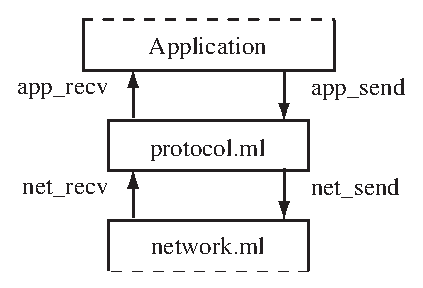
\includegraphics{network_stack}
\end{center}
%
With this design, the \hbox{\lstinline+Network+} component
calls \hbox{\lstinline+Protocol.net_recv+} when a message arrives, and
the \hbox{\lstinline+Protocol+} component
calls \hbox{\lstinline+Network.net_send+} to send a message.  However,
this is not possible if the implementations are in separate
files \hbox{\lstinline+protocol.ml+} and \hbox{\lstinline+network.ml+}
because that would introduce a cyclic dependency.

Describe a method to circumvent this problem, without placing the code
for the two components into a single file.

\begin{answer}\ifanswers
There are a few potential solutions, including the use of recursive
modules (discussed in Section~\ref{section:recursive-modules}) or
objects (Chapter~\ref{chapter:objects}).  In addition here are a few
alternate ways.

\begin{enumerate}
\item

If the design can be partitioned into two separate message streams
without any cycles, the design can be programmed directly.

\begin{center}
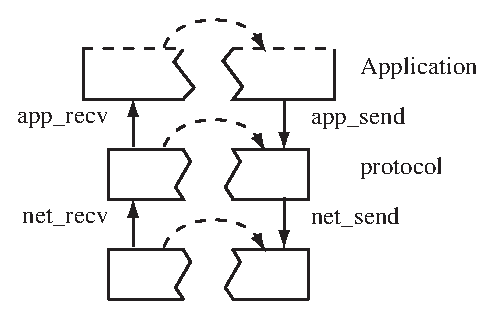
\includegraphics{network_stack2}
\end{center}
%
However, this approach may not be possible, and the changes required
may be unnatural.

\item

A simpler solution is to introduce a third file containing references
that can be set to refer each of the functions.  This solution, while
lacking elegance, is straightforward.

\begin{center}
\begin{tabular}{l}
refs.mli\\
\hline
\begin{minipage}{5in}
\begin{ocaml}
val net_recv_ref : (message -> unit) ref
val net_send_ref : (message -> unit) ref
val app_recv_ref : (message -> unit) ref
val app_send_ref : (message -> unit) ref
\end{ocaml}
\end{minipage}
\end{tabular}
\end{center}
%
The cells are initialized with dummy values.
\begin{ocaml}
let net_recv_ref = ref (fun _ -> raise (Invalid_argument "not initialized"))
...
\end{ocaml}
%
At startup time, the layers set the references to refer to the
appropriate functions.

\begin{center}
\begin{tabular}{l}
protocol.ml\\
\hline
\begin{minipage}{3in}
\begin{ocaml}
let net_recv msg = ...
...
Refs.net_recv_ref := net_recv
\end{ocaml}
\end{minipage}
\end{tabular}
\end{center}

\item

Yet another option is to define a third file,
say \hbox{\lstinline+link.ml+} that builds the recursive definition in
a single file.  Each of the layer functions would take as arguments
the functions that it expects to call.

\begin{ocaml}
let rec net_recv msg =
   Protocol.net_recv net_send app_recv msg
and app_send msg =
   Protocol.app_send net_send app_recv msg
and net_send msg =
   Network.net_send net_recv msg
and app_recv msg =
   Application.app_recv app_send msg
\end{ocaml}
%
This solution is more complicated and may be slightly less efficient
than the solution using reference cells.

\end{enumerate}
\fi\end{answer}
\end{exercise}

% -*-
% Local Variables:
% Mode: LaTeX
% fill-column: 100
% TeX-master: "paper"
% TeX-command-default: "LaTeX/dvips Interactive"
% End:
% -*-
% vim:tw=100:fo=tcq:

%
%
%

\labelchapter{modules}{The OCaml Module System}

\index{modules}
As we saw in the previous chapter, programs can be divided into parts
that can be implemented in files, and each file can be given an
interface that specifies what its public types and values are. Files
are not the only way to partition a program, OCaml also provides
a \emph{module system} that allows programs to be partitioned even
within a single file. There are three key parts in the module
system: \emph{signatures}, \emph{structures}, and \emph{functors},
where signatures correspond to interfaces, structures correspond to
implementations, and functors are functions over structures. In this
chapter, we will discuss the first two; we'll leave discussion of
functors to Chapter~\reflabelchapter{functors}.

There are several reasons for using the module system. Perhaps the
simplest reason is that each structure has its own namespace, so name
conflicts are less likely when modules are used.  Another reason is
that abstraction can be specified explicitly within a file by
assigning a signature to a structure.  Let's begin with naming.

\labelsection{structures}{Structures and signatures}

\label{keyword:module}
\label{keyword:struct}
\index{structures}
\index{module|see{modules}@\lstinline$module$}
\index{struct@\lstinline$struct$}
Named structures are defined with the \lstinline{module} and
\lstinline{struct} keywords using the following syntax.

\begin{ocaml}
module $\nt{ModuleName}$ = struct $\nt{implementation}$ end
\end{ocaml}
%
\index{identifiers!module}
The module name \nt{ModuleName} must begin with an uppercase
letter.  The \nt{implementation} can include any definition
that might occur in a \hbox{\lstinline/.ml/} file.

In the discussion of records (page~\pageref{section:record-labels}), we
noted that the space of record label names is flat; if two record
types are defined with the same label names in the same file, the
first definition is lost.  Modules solve this problem by allowing the
name space to be partitioned.  Here is an example using records; the
same principle applies to unions and constructor names.

\begin{ocaml}
module A = struct
    type t = { name : string; phone : string }
end
module B = struct
    type t = { name : string; salary : float }
end
# let jason = { A.name = "Jason"; A.phone = "626-555-1212" };;
@
\begin{topoutput}
val jason : A.t = {A.name = "Jason"; A.phone = "626-555-1212"}
\end{topoutput}
@
# let bob = { B.name = "Bob"; B.salary = 180.0 };;
@
\begin{topoutput}
val bob : B.t = {B.name = "Bob"; B.salary = 180.}
\end{topoutput}
@
\end{ocaml}
%
\index{fully-qualified names}
A simple \emph{pathname}, or \emph{fully-qualified} name, has the
syntax \nt{ModuleName}.\nt{identifier}, where the \nt{identifier} is
the name of a module component (a type, value, record label, a nested
module, etc.), and the \nt{ModuleName} is the module containing the
component.  In the example, the pathname \hbox{\lstinline$B.salary$}
is the fully-qualified name of a field in the \hbox{\lstinline$B.t$}
record type (which is also a fully-qualified name).

Let's return to the \hbox{\lstinline/unique.ml/} example from the
previous chapter, using a simple list-based implementation of
sets. This time, instead of defining the set data structure in a
separate file, let's define it as a module,
called \hbox{\lstinline/Set/}, using an explicit module
definition. The program is shown in Figure~\reffigure{xmset1}.  The
file is compiled and executed using the usual methods.

\begin{figure}
\begin{center}
\begin{tabular}[t]{l}
File: unique.ml\\
\hline
\begin{ocamllisting}
module Set = struct
   let empty = []
   let add x l = x :: l
   let mem x l = List.mem x l
end;;

let rec unique already_read =
   output_string stdout "> ";
   flush stdout;
   let line = input_line stdin in
      if not (Set.mem line already_read) then begin
         output_string stdout line;
         output_char stdout '\n';
         unique (Set.add line already_read)
      end else
         unique already_read;;

(* Main program *)
try unique Set.empty with
   End_of_file ->
      ();;
\end{ocamllisting}
\end{tabular}
\end{center}
\caption{Gathering the \hbox{\lstinline$Set$} implementation into a module.}
\labelfigure{xmset1}
\end{figure}

\begin{ocaml}
% ocamlc -o unique unique.ml
% ./unique
> Adam Bede
@
\begin{topoutput}
Adam Bede
\end{topoutput}
@
> A passage to India
@
\begin{topoutput}
A Passage to India
\end{topoutput}
@
> Adam Bede
> Moby Dick
@
\begin{topoutput}
Moby Dick
\end{topoutput}
@
\end{ocaml}
%
In this new program, the main role of the
module \hbox{\lstinline/Set/} is to collect the set functions into a
single block of code that has an explicit name. The values are now
named using the module name as a prefix,
as \hbox{\lstinline/Set.empty/}, \hbox{\lstinline/Set.add/},
and \hbox{\lstinline/Set.mem/}. Otherwise, the program is as before.

\label{keyword:sig}
\index{signatures}
\index{abstraction!for modules}
In many ways, structures are like files.  If we wish to hide
the \hbox{\lstinline$Set$} implementation, we can specify an explicit
signature to hide parts of the implementation.  A named signature is
defined with a \hbox{\lstinline/module type/} definition.

\begin{ocaml}
module type $\nt{ModuleName}$ = sig $\nt{signature}$ end
\end{ocaml}
%
The name of the signature must begin with an uppercase letter. The
signature can contain any of the items that can occur in an
interface \hbox{\lstinline/.mli/} file. For our example, the signature
should include an abstract type declaration for
the \hbox{\lstinline/'a set/} type and \hbox{\lstinline/val/}
declarations for each of the values. The \hbox{\lstinline/Set/}
module's signature is constrained by specifying the signature after a
colon in the module definition
%
\hbox{\lstinline/module Set : SetSig = struct $\cdots$ end/},
%
as shown in Figure \reffigure{xmset2}.

\begin{figure}
\begin{center}
\begin{tabular}{ll}
\begin{tabular}[t]{l}
Signature definition\\
\hline
\begin{ocamllisting}
module type SetSig = sig
   type 'a set
   val empty : 'a set
   val add : 'a -> 'a set -> 'a set
   val mem : 'a -> 'a set -> bool
end;;
\end{ocamllisting}
\end{tabular}
&
\begin{tabular}[t]{l}
Structure definition\\
\hline
\begin{ocamllisting}
module Set : SetSig = struct
   type 'a set = 'a list
   let empty = []
   let add x l = x :: l
   let mem x l = List.mem x l
end;;
\end{ocamllisting}
\end{tabular}
\end{tabular}
\end{center}
\caption{Defining an explicit signature for the \hbox{\lstinline$Set$} module.}
\labelfigure{xmset2}
\end{figure}

\labelsection{module-contents}{Module definitions}

In general, structures and signatures are just like implementation
files and their interfaces. Structures are allowed to contain any of
the definitions that might occur in a implementation, including any of
the following.

\begin{itemize}
\item \lstinline$type$ definitions
\item \lstinline$exception$ definitions
\item \lstinline$let$ definitions
\item \lstinline$open$ statements to open the namespace of another module
\item \lstinline$include$ statements that include the contents of another module
\item signature definitions
\item nested structure definitions
\end{itemize}
%
Similarly, signatures may contain any of the declarations that might
occur in an interface file, including any of the following.

\begin{itemize}
\item \lstinline$type$ declarations
\item \lstinline$exception$ definitions
\item \lstinline$val$ declarations
\item \lstinline$open$ statements to open the namespace of another signature
\item \lstinline$include$ statements that include the contents of another signature
\item nested signature declarations
\end{itemize}
%

\labelsubsection{modules-first-class}{Modules are not first-class}

\index{modules!not first class}
Modules/structures/signatures are not \emph{first-class}, meaning in
particular that they are not expressions.  Modules cannot be passed as
arguments to a function nor can they be returned as results.
Normally, modules are defined as top-level outermost components in a
program, hence all type and exception definitions are also top-level.

\index{phase distinction} There are several reasons why modules are not first-class.  Perhaps the
most important is that modules and module types are complicated expressions involving types and type
abstraction; if modules could be passed as values, type inference would become undecidable.  Another
reason is called the \emph{phase-distinction}.  From the point of view of the compiler, a program
has two phases in its lifetime: compile-time and run-time.  The objective of the phase distinction
is to ensure that module expressions can be computed at compile-time.  If modules were expressions,
the phase-distinction would be difficult to ensure.  In any case, the phase distinction is simply a
guideline for the language designers.  The effect on programmers is that modules can only be defined
in a few chosen locations, but there is no performance penalty for using them.

\labelsubsection{letmodule}{The \hbox{\lstinline$let module$} expression}

\index{let module@\lstinline$let module$}
\index{modules!local definitions@local definitions using \lstinline$let$}
One exception to top-level module definitions is the
%
\hbox{\lstinline$let module$}
%
expression, which has the following syntax.

\begin{ocaml}
let module $\nt{ModuleName}$ = $\nt{module\_expression}$ in $\nt{body\_expression}$
\end{ocaml}
%
The \nt{module\_expression} is the definition of a module
(often a \hbox{\lstinline/struct $\cdots$ end/} block), and the module is
defined in the \nt{body\_expression}.  The
%
\hbox{\lstinline$let module$}
%
expression is frequently used for renaming modules locally.

\begin{ocaml}
module ModuleWithALongName
...
let f x =
   let module M = ModuleWithALongName in
   ...
\end{ocaml}
%
Similarly, it can be useful sometimes to redefine an existing module
locally.  In the following example, a \hbox{\lstinline$String$} module is
defined so that pathnames \lstinline{String.$\ms{identifier}$} in the
\texttt{\emph{function body}} refer to the locally-defined module, not the
standard library (in this case, it is for debugging purposes).

\begin{ocaml}
let f x =
   let module String = struct
      let create n =
          eprintf "Allocating a string of length %d\n%!" n;
          String.create n
      ...
   end in
   @\emph{function body}@
\end{ocaml}
%
One other use of \hbox{\lstinline/let module/} expression is to allow
types and exceptions to be defined locally, not only at the top-level.  For
example, in the following program, the
exception \hbox{\lstinline/Error/} is local.  It is guaranteed to be
different from every other exception in the program.

\begin{ocaml}
let f x =
   let module M = struct exception Abort end in
   let g y =
      ...
      if $\ms{done}$ then raise M.Abort
   in
   try map g x with
      M.Abort message -> ...
\end{ocaml}
%
In this particular case, the local definition of
the \hbox{\lstinline$M.Abort$} exception means that
the \hbox{\lstinline$map$} function (not shown) is not able to catch
the exception except generically, by catching all exceptions.

\labelsection{recursive-modules}{Recursive modules}

\index{and!recursive modules}
\index{rec!for recursive modules}
\index{modules!recursive}
It is also possible to define modules that are defined recursively.
That is, several modules that refer to one another are defined at
once.  The syntax for a recursive definition uses
the \lstinline{module rec} form.

\begin{ocaml}
module rec $\nt{Name}_1$ : $\nt{Signature}_1$ = $\nt{struct\_expression}_1$
and $\nt{Name}_2$ : $\nt{Signature}_2$ = $\nt{struct\_expression}_2$
$\vdots$
and $\nt{Name}_n$ : $\nt{Signature}_n$ = $\nt{struct\_expression}_n$
\end{ocaml}
%
The signatures $\nt{Signature}_i$ are \emph{required}.

For example, let's build a kind of nonempty trees with unbounded
branching, and a function \hbox{\lstinline$map$} with the standard
meaning.  The \hbox{\lstinline$map$} function could be defined as part
of a single module, but it is also possible to use recursive modules
to split the program into two parts 1) mapping over single tree nodes,
and 2) mapping over lists of trees.

\begin{ocaml}
type 'a ubtree = Node of 'a * 'a ubtree list

module rec Tree : sig
   val map : ('a -> 'b) -> 'a ubtree -> 'b ubtree
end = struct
   let map f (Node (x, children)) =
      Node (f x, Forest.map f children)
end

and Forest : sig
   val map : ('a -> 'b) -> 'a ubtree list -> 'b ubtree list
end = struct
   let map f l =
      List.map (Tree.map f) l
end;;
\end{ocaml}
%
This definition is necessarily recursive because
the \hbox{\lstinline$Tree$} module refers
to \hbox{\lstinline$Forest.map$}, and \hbox{\lstinline$Forest$} refers
to \hbox{\lstinline$Tree.map$}.

The signatures are required---one way to think of it is that the types
of the mutual references are needed so that type checking can be
performed for each module in isolation.\footnote{Recursive modules are
relatively new to OCaml; these requirements may change.}
Stylistically, recursive modules are used infrequently for simple
structure definitions; they become much more useful when used with
functors, which allow the module bodies to be placed in separate
files.

\labelsection{include}{The \hbox{\lstinline$include$} directive}

\label{keyword:include}
\index{include!module inclusion}
\index{modules!include@\lstinline$include$}
We have seen most of the module components before.  However, one new
construct we haven't seen is \hbox{\lstinline/include/}, which allows
the entire contents of a structure or signature to be included in
another.  The \hbox{\lstinline/include/} statement can be used to
create modules and signatures that re-use existing definitions.

\labelsubsection{include-extend}{Using include to extend modules}

Suppose we wish to define a new kind of sets \hbox{\lstinline/ChooseSet/} that has a
\hbox{\lstinline/choose/} function that returns an element of the set if one exists. Instead of
re-typing the entire signature, we can use the \hbox{\lstinline/include/} statement to include the
existing signature, as shown in Figure~\reffigure{xmset3}. The resulting signature includes all of
the types and declarations from \hbox{\lstinline/SetSig/} as well as the new function declaration
\hbox{\lstinline/val choose/}. For this example, we are using the toploop to display the inferred
signature for the new module.

\begin{figure}
\begin{center}
\begin{tabular}{ll}
\begin{tabular}[t]{l}
Signature definition\\
\hline
\begin{ocamllisting}
module type ChooseSetSig = sig
   include SetSig
   val choose : 'a set -> 'a option
end;;
\end{ocamllisting}
\end{tabular}
&
\begin{tabular}[t]{l}
Inferred type\\
\hline
\begin{ocamllisting}
module type ChooseSetSig = sig
   type 'a set
   val empty : 'a set
   val add : 'a -> 'a set -> 'a set
   val mem : 'a -> 'a set -> bool
   val choose : 'a set -> 'a option
end;;
\end{ocamllisting}
\end{tabular}
\end{tabular}
\end{center}
\caption{Extending a signature with \hbox{\lstinline+include+}.}
\labelfigure{xmset3}
\end{figure}

\labelsubsection{include-struct}{Using include to extend implementations}

The \texttt{include} statement can also be used in
implementations. For our example, however, there is a problem. The
straightforward approach in defining a
module \hbox{\lstinline/ChooseSet/} is to include
the \hbox{\lstinline/Set/} module, then define the new
function \hbox{\lstinline/choose/}. The result of this attempt is
shown in Figure \reffigure{xmset4}, where the toploop prints out an
extensive error message (the toploop prints out the full signature,
which we have elided in \hbox{\lstinline/sig $\cdots$ end/}).

\begin{figure}
\begin{center}
\begin{tabular}{ll}
\begin{tabular}[t]{l}
Structure definition\\
\hline
\begin{ocamllisting}
module ChooseSet
 : ChooseSetSig =
struct
   include Set
   let choose = function
      x :: _ -> Some x
    | [] -> None
end;;
\end{ocamllisting}
\end{tabular}
&
\begin{tabular}[t]{l}
Inferred type (from the toploop)\\
\hline
\begin{ocaml}
@
\begin{toperror}
Signature mismatch:
Modules do not match:
   sig ... end
is not included in
   ChooseSetSig
Values do not match:
   val choose : 'a list -> 'a option
   val choose : 'a set -> 'a option
\end{toperror}
@
\end{ocaml}
\end{tabular}
\end{tabular}
\end{center}
\caption{A failed attempt to extend the \hbox{\lstinline/Set/} implementation.}
\labelfigure{xmset4}
\end{figure}
%
The problem is apparent from the last few lines of the error
message---the \hbox{\lstinline/choose/} function has
type \hbox{\lstinline/'a list -> 'a option/}, not
\hbox{\lstinline/'a set -> 'a option/}
as it should. The issue is that we included the \emph{abstract}
module \hbox{\lstinline/Set/}, where the type
\hbox{\lstinline/'a set/}
has an abstract type, not a list.

One solution is to manually copy the code from
the \hbox{\lstinline/Set/} module into
the \hbox{\lstinline/ChooseSet/} module. This has its drawbacks of
course. We aren't able to re-use the existing implementation, our code
base gets larger, etc.  If we have access to the original non-abstract
set implementation, there is another solution---we can just include
the non-abstract set implementation, where it is known that the set is
represented as a list.

Suppose we start with a non-abstract
implementation \hbox{\lstinline/SetInternal/} of sets as lists. Then
the module \hbox{\lstinline/Set/} is the same implementation, with the
signature \hbox{\lstinline/SetSig/}; and
the \hbox{\lstinline/ChooseSet/} includes
the \hbox{\lstinline/SetInternal/} module instead
of \hbox{\lstinline/Set/}. Figure~\reffigure{xmset5} shows the
definitions in this order, together with the types inferred by the
toploop.

\begin{figure}
\begin{center}
\begin{tabular}{ll}
\begin{tabular}[t]{l}
Structure definitions\\
\hline
\begin{ocamllisting}
module SetInternal = struct
   type 'a set = 'a list
   let empty = []
   let add x l = x :: l
   let mem x l = List.mem x l
end;;

module Set : SetSig = SetInternal

module ChooseSet
 : ChooseSetSig =
 struct
   include SetInternal
   let choose = function
      x :: _ -> Some x
    | [] -> None
end;;
\end{ocamllisting}
\end{tabular}
&
\begin{tabular}[t]{l}
Inferred types (from the toploop)\\
\hline
\begin{ocamllisting}
module SetInternal : sig
   type 'a set = 'a list
   val empty : 'a list
   val add : 'a -> 'a list -> 'a list
   val mem : 'a -> 'a list -> bool
end;;

module Set : SetSig

module ChooseSet : ChooseSetSig
\end{ocamllisting}
\end{tabular}
\end{tabular}
\end{center}
\caption{Extending the \hbox{\lstinline/Set/} using an internal specification.}
\labelfigure{xmset5}
\end{figure}

Note that for the module \hbox{\lstinline/Set/} it is not necessary to
use a \hbox{\lstinline/struct $\cdots$ end/} definition because
the \hbox{\lstinline/Set/} module is \emph{equivalent} to
the \hbox{\lstinline/SetInternal/} module, it just has a different
signature. The modules \hbox{\lstinline/Set/}
and \hbox{\lstinline/ChooseSet/} are ``friends,'' in that they share
internal knowledge of each other's implementation, while keeping their
public signatures abstract.

\labelsection{module-hiding}{Abstraction, friends, and module hiding}

\index{abstraction}
\index{modules!abstraction}
So far, we have seen that modules provide two main features, 1) the
ability to divide a program into separate program units (modules) that
each have a separate namespace, and 2) the ability to assign
signatures that make each structure partially or totally abstract. In
addition, as we have seen in the previous example, a structure
like \hbox{\lstinline/SetInternal/} can be given more than one
signature (the module \hbox{\lstinline/Set/} is equal
to \hbox{\lstinline/SetInternal/} but it has a different signature).

Another frequent use of modules uses nesting to define multiple levels
of abstraction. For example, we might define a module container in
which several modules are defined and implementation are visible, but
the container type is abstract. This is akin to the C++ notion of
``friend'' classes, where a set of friend classes may mutually refer
to class implementations, but the publicly visible fields remain
protected.

In our example, there isn't much danger in leaving
the \hbox{\lstinline/SetInternal/} module publicly
accessible. A \hbox{\lstinline/SetInternal.set/} can't be used in
place of a \hbox{\lstinline/Set.set/} or
a \hbox{\lstinline/ChooseSet.set/}, because the latter types are
abstract. However, there is a cleaner solution that nests
the \hbox{\lstinline/Set/} and \hbox{\lstinline/ChooseSet/} structures
in an outer \hbox{\lstinline/Sets/} module. The signatures are left
unconstrained within the \hbox{\lstinline/Sets/} module, allowing
the \hbox{\lstinline/ChooseSet/} structure to refer to the
implementation of the \hbox{\lstinline/Set/} structure, but the
signature of the \hbox{\lstinline/Sets/} module is constrained. The
code for this is shown in Figure\reffigure{xmset6}.

\begin{figure}
\begin{center}
\begin{tabular}{ll}
\begin{tabular}[t]{l}
Module definitions\\
\hline
\begin{ocamllisting}
module Sets : sig
   module Set : SetSig
   module ChooseSet : ChooseSetSig
end = struct
   module Set = struct
      type 'a set = 'a list
      let empty = []
      let add x l = x :: l
      let mem x l = List.mem x l
   end
   module ChooseSet = struct
      include Set
      let choose = function
         x :: _ -> Some x
       | [] -> None
   end
end;;
\end{ocamllisting}
\end{tabular}
&
\begin{tabular}[t]{l}
Inferred types (from the toploop)\\
\hline
\begin{ocamllisting}
module Sets : sig
   module Set : SetSig
   module ChooseSet : ChooseSetSig
end
\end{ocamllisting}
\end{tabular}
\end{tabular}
\end{center}
\caption{Defining \misspelled{\texttt{ChooseSet}} and \texttt{Set} as friends.}
\labelfigure{xmset6}
\end{figure}

There are a few things to note for this definition.

\begin{enumerate}
\item{}

The \hbox{\lstinline/Sets/} module uses an \emph{anonymous} signature
(meaning that the signature has no name). Anonymous signatures
and \textbf{struct} implementations are perfectly acceptable any place
where a signature or structure is needed.

\item{}

Within the \hbox{\lstinline/Sets/} module the \hbox{\lstinline/Set/}
and \hbox{\lstinline/ChooseSet/} modules are not constrained, so that
their implementations are public. This allows
the \hbox{\lstinline/ChooseSet/} to refer to
the \hbox{\lstinline/Set/} implementation directly (so in this case,
the \hbox{\lstinline/Set/} and \hbox{\lstinline/ChooseSet/} modules
are friends). The signature for the \hbox{\lstinline/Sets/} module
makes them abstract.

\end{enumerate}

\labelsubsection{incompatible-include}{Using include with incompatible signatures}

\index{include!incompatible signatures}
In our current example, it might seem that there isn't much need to
have two separate modules \hbox{\lstinline/ChooseSet/}
(with \hbox{\lstinline/choice/}) and \hbox{\lstinline/Set/}
(without \hbox{\lstinline/choice/}). In practice it is perhaps more
likely that we would simply add a \hbox{\lstinline/choice/} function
to the \hbox{\lstinline/Set/} module. The addition would not affect
any existing code, since any existing code doesn't refer to
the \hbox{\lstinline/choice/} function anyway.

Surprisingly, this kind of example occurs in practice more than it
might seem, due to programs being developed with incompatible
signatures. For example, suppose we are writing a program that is
going to make use of two independently-developed libraries. Both
libraries have their own \hbox{\lstinline/Set/} implementation, and we
decide that we would like to use a single \hbox{\lstinline/Set/}
implementation in the combined program. Unfortunately, the signatures
are incompatible---in the first library, the \hbox{\lstinline/add/}
function was defined with type
\hbox{\lstinline/val add : 'a -> 'a set -> 'a set/};
but in the second library, it was defined with
type \hbox{\lstinline/val add : 'a set -> 'a -> 'a set/}. Let's say
that the first library uses the desired signature. Then, one solution
would be to hunt through the second library, finding all calls to
the \hbox{\lstinline/Set.add/} function, reordering the arguments to
fit a common signature. Of course, the process is tedious, and it is
unlikely we would want to do it.

An alternative is to \emph{derive} a wrapper
module \hbox{\lstinline/Set2/} for use in the second library. The
process is simple, 1) \hbox{\lstinline/include/}
the \hbox{\lstinline/Set/} module, and 2) redefine
the \hbox{\lstinline/add/} to match the desired signature; this is
shown in Figure~\reffigure{xmset7}.

\begin{figure}
\begin{center}
\begin{tabular}{ll}
\begin{tabular}[t]{l}
Signature\\
\hline
\begin{ocamllisting}
module type Set2Sig = sig
   type 'a set
   val empty : 'a set
   val add : 'a set -> 'a -> 'a set
   val mem : 'a -> 'a set -> bool
end;;
\end{ocamllisting}
\end{tabular}
&
\begin{tabular}[t]{l}
Implementation\\
\hline
\begin{ocamllisting}
module Set2 : Set2Sig = struct
   include Set
   let add l x = Set.add x l
end;;
\end{ocamllisting}
\end{tabular}
\end{tabular}
\end{center}
\caption{Wrapping a module to use a new signature.}
\labelfigure{xmset7}
\end{figure}

The \hbox{\lstinline/Set2/} module is just a wrapper. Apart from
the \hbox{\lstinline/add/} function, the types and values in
the \hbox{\lstinline/Set/} and \hbox{\lstinline/Set2/} modules are the
same, and the \hbox{\lstinline/Set2.add/} function simply reorders the
arguments before calling the \hbox{\lstinline/Set.add/}
function. There is little or no performance penalty for the
wrapper---in most cases the native-code OCaml compiler
will \emph{inline} the \hbox{\lstinline/Set2.add/} function (in other
words, it will perform the argument reordering at compile time).

\labelsection{sharing-constraints}{Sharing constraints}

There is one remaining problem with this example. In the combined
program, the first library uses the original \hbox{\lstinline/Set/}
module, and the second library uses \hbox{\lstinline/Set2/}. It is
likely that we will want to pass values, including sets, from one
library to the other. However, as defined, the 
\hbox{\lstinline/'a Set.set/}
and \hbox{\lstinline/'a Set2.set/} types are distinct abstract types,
and it is an error to use a value of type 
\hbox{\lstinline/'a Set.set/}
in a place where a value of type \hbox{\lstinline/'a Set2.set/} is
expected, and \textit{vice-versa}. The following error message is
typical.

\begin{ocaml}
# Set2.add Set.empty 1;;
@
\begin{toperror}
This expression has type 'a Set.set
   but is here used with type 'b Set2.set
\end{toperror}
@
\end{ocaml}
%
Of course, we might want the types to be distinct. But in this case,
it is more likely that we want the definition to be transparent. We
know that the two kinds of sets are really the
same---\hbox{\lstinline/Set2/} is really just a wrapper
for \hbox{\lstinline/Set/}. How do we establish the equivalence
of \hbox{\lstinline/'a Set.set/} and \hbox{\lstinline/'a Set2.set/}?

\index{sharing constraints|see{modules}}
\index{modules!sharing constraints}
The solution is called a \emph{sharing constraint}. The syntax for a
sharing constraint uses the \hbox{\lstinline/with/} keyword to specify
a type equivalence for a module signature in the following form.

\begin{ocaml}
$\nt{signature}$ ::= $\nt{signature}$ with type $\nt{typename}$ = $\nt{type}$
\end{ocaml}
%
In this particular case, we wish to say that the
%
\hbox{\lstinline/'a Set2.set/}
%
type is equal to the \hbox{\lstinline/'a Set.set/} type, which we can
do by adding a sharing constraint when the \hbox{\lstinline/Set2/}
module is defined, as shown in Figure \reffigure{xmset8}.

\begin{figure}
\begin{center}
\begin{tabular}{ll}
\begin{tabular}[t]{l}
Module definition\\
\hline
\begin{ocamllisting}
module Set2 : Set2Sig
   with type 'a set = 'a Set.set =
struct
   include Set
   let add l x = Set.add x l
end;;
\end{ocamllisting}
\end{tabular}
&
\begin{tabular}[t]{l}
Toploop\\
\hline
\begin{ocaml}
# let s = Set2.add Set.empty 1;;
@
\begin{topoutput}
val s : int Set2.set = <abstr>
\end{topoutput}
@
# Set.mem 1 s;;
@
\begin{topoutput}
- bool = true
\end{topoutput}
@
\end{ocaml}
\end{tabular}
\end{tabular}
\end{center}
\caption{Defining a sharing constraint.}
\labelfigure{xmset8}
\end{figure}
%
The constraint specifies that the types \hbox{\lstinline/'a Set2.set/}
and \hbox{\lstinline/'a Set.set/} are the same. In other words,
they \emph{share} a common type. Since the two types are equal, set
values can be freely passed between the two set implementations.

% -*-
% Local Variables:
% Mode: LaTeX
% fill-column: 100
% TeX-master: "paper"
% TeX-command-default: "LaTeX/dvips Interactive"
% End:
% -*-

%
%
%

%%%%%%%%%%%%%%%%%%%%%%%%%%%%%%%%%%%%%%%%%%%%%%%%%%%%%%%%%%%%%%%%%%%%%%%%
% Exercises
%
\exercises

\begin{exercise}{struct1}
Which of the following are legal programs?  Explain your answers.
\begin{enumerate}
\item

\begin{ocamllisting}
module A : sig
   val x : string
end = struct
   let x = 1
   let x = "x"
end
\end{ocamllisting}

\item

\begin{ocamllisting}
module A : sig
   val x : string
   val x : string
end = struct
   let x = "x"
end
\end{ocamllisting}

\item

\begin{ocamllisting}
module a = struct
   let x = 1
end;;
\end{ocamllisting}

\item

\begin{ocamllisting}
module M : sig
   val f : int -> int
   val g : string -> string
end = struct
   let g x = x
   let f x = g x
end
\end{ocamllisting}

\item

\begin{ocamllisting}
let module X = struct let x = 1 end in X.x
\end{ocamllisting}

\item

\begin{ocamllisting}
module M = struct
   let g x = h x
   let f x = g x
   let h x = x + 1
end
\end{ocamllisting}

\item

\begin{ocamllisting}
module rec M : sig
   val f : int -> int
   val h : int -> int
end = struct
   open M
   let g x = h x
   let f x = g x
   let h x = x + 1
end
\end{ocamllisting}

\item

\begin{ocamllisting}
module rec M : sig
   val f : int -> int
end = struct
   let f = M.f
end
\end{ocamllisting}

\item

\begin{ocamllisting}
type 'a t = { set : 'a -> unit; get : unit -> 'a }
let f x =
   let cell = ref x in
   let module M = struct
      let s i = cell := i
      let g () = !cell
      let r = { set = s; get = g }
   end
   in
      M.r
\end{ocamllisting}

\item

\begin{ocamllisting}
let f x =
   let cell = ref x in
   let module M = struct
      type 'a t = { set : 'a -> unit; get : unit -> 'a }
      let s i = cell := i
      let g () = !cell
      let r = { set = s; get = g }
   end
   in
      M.r
\end{ocamllisting}

\item

\begin{ocamllisting}
module type ASig = sig type s  val f : int -> s end
module type BSig = sig type t  val g : t -> int end
module C : sig
   module A : ASig
   module B : BSig with type t = A.s
end = struct
   type u = string
   module A = struct type s = u  let f = string_of_int end
   module B = struct type t = u  let g = int_of_string end
end
include C
let i = B.g (A.f ())
\end{ocamllisting}   

\item

\begin{ocamllisting}
module type ASig = sig type t end
module type BSig = sig val x : int end
module A : ASig with type t = int
   = struct type t = int end
module B : BSig = struct let x = 1 end
module C : sig
   include ASig
   val x : t
end = struct
   include A
   include B
end
\end{ocamllisting}
\end{enumerate}

\begin{answer}\ifanswers
\begin{enumerate}
\item

Legal; the value associated with a variable is specified by the last
definition in the module.
\item 

Legal; the duplicate type definition is legal.  What would happen if
the type definitions differ?
\item 

Not legal; the module name must begin with an uppercase letter.
\item 

Legal; within the structure body the function \hbox{\lstinline/g/} has
type \hbox{\lstinline$'a -> 'a$}.  The type constraint is
applied \emph{after} the structure is formed.
\item 

Legal; the value is \hbox{\lstinline$1$}.
\item 

Not legal; the function \hbox{\lstinline/h/} must be defined before \hbox{\lstinline/g/}.
\item 

Legal; the forward reference to \hbox{\lstinline$h x$} is allowed
because the module is recursive.
\item 

Legal; however a application of the function \hbox{\lstinline/f/} will fail at
runtime because the value cannot be resolved.
\item 

Legal; \hbox{\lstinline/f/} has type \hbox{\lstinline$f : 'a -> 'a t$}.
\item

Not legal; OCaml produces the error message ``In this type, the
locally bound module name M escapes its scope.''  This is because the
the function \hbox{\lstinline/f/} produces a value of type \hbox{\lstinline$M.t$},
but \hbox{\lstinline$M$} is defined only in the body of \hbox{\lstinline/f/}.

\item

Legal; the modules \hbox{\lstinline/A/} and \hbox{\lstinline/B/} share a common (abstract) type,
so it is legal to pass the result of \lstinline $A.f$
t \hbox{\lstinline$B.g$}.

\item

Legal; the \hbox{\lstinline$include$} directive is like textual inclusion,
subject to signature constraints.  After expansion, the module \hbox{\lstinline/C/}
has the following form.

\begin{ocaml}
module C : sig
   type t
   val x : t
end = struct
   type t = int (* sig type t = int *)
   let x = 1    (* sig val x : int *)
end
\end{ocaml}
%
This is a legal module definition.
\end{enumerate}
\fi\end{answer}
\end{exercise}

%%%%%%%%%%%%%%%%%%%%%%%%%%%%%%%%%%%%%%%%%%%%%%%%%%%%%%%%%%%%%%%%%%%%%%%%
%
%
\begin{exercise}{struct1}
In OCaml, programs are usually written ``bottom-up,'' meaning that
programs are constructed piece-by-piece, and the last function is a
file is likely to be the most important.  Many programmers prefer a
top-down style, where the most important functions are defined first
in a file, and supporting definitions are placed later in the file.
Can you use the module system to allow top-down programming?

\begin{answer}\ifanswers
Recursive modules can be used for the top-down programming style.  The
code is wrapped in a module, and all forward references must be
declared in the module signature.  To illustrate, suppose we have a
function \hbox{\lstinline$main$} that calls
functions \hbox{\lstinline$f$} and \hbox{\lstinline$g$}, using an
intermediate type \hbox{\lstinline$t$}.

\begin{ocaml}
module rec Body : sig
   type t = V of int
   val main : int -> int
   val f : int -> t
   val g : t -> int
end = struct
   open Body

   let main i = g (f i)
   let f i = V i
   let g (V i) = i
   type t = V of int
end
\end{ocaml}
%
This approach has the usual disadvantage that types must be defined
twice, once in the signature and once in the structure.  However, the
type definition can be defined before the module.  This is common
style even in top-down programming.
\fi\end{answer}
\end{exercise}

%%%%%%%%%%%%%%%%%%%%%%%%%%%%%%%%%%%%%%%%%%%%%%%%%%%%%%%%%%%%%%%%%%%%%%%%
% 
%
\begin{exercise}{struct2}
One could argue that sharing constraints are never necessary for
unparameterized modules like the ones in this chapter. In the example
of Figure~\reffigure{xmset8}, there are at least two other solutions
that allow the \hbox{\lstinline/Set2/} and \hbox{\lstinline/Set/}
modules to share values, without having to use sharing
constraints. Present two alternate solutions without sharing
constraints.
\end{exercise}

\begin{exercise}{struct3}
In OCaml, signatures can apparently contain multiple declarations for the same value.

\begin{ocaml}
# module type ASig = sig
   val f : 'a -> 'a
   val f : int -> int
  end;;
@
\begin{topoutput}
module type ASig = sig val f : 'a -> 'a val f : int -> int end
\end{topoutput}
@
\end{ocaml}
%
In any structure that is given this signature, the
function \hbox{\lstinline$f$} must have \emph{all} the types listed.
If \hbox{\lstinline$f$} is not allowed to raise an exception, what is
the only sensible definition for it?

\begin{answer}\ifanswers
Instead of using a sharing constraint, we can add the type definition
directly in the signature.

\begin{ocaml}
module type Set2Sig = sig
   type 'a set = 'a Set.set
   val empty : 'a set
   ...
end
\end{ocaml}
%
In fact, we don't even need to define a separate type.

\begin{ocaml}
module type Set2Sig = sig
   val empty : 'a Set.set
   val add : 'a Set.set -> 'a -> 'a Set.set
   val mem : 'a -> 'a Set.set -> bool
end
\end{ocaml}
\fi\end{answer}
\end{exercise}

%%%%%%%%%%%%%%%%%%%%%%%%%%%%%%%%%%%%%%%%%%%%%%%%%%%%%%%%%%%%%%%%%%%%%%%%
% 
%
\begin{exercise}{struct4}
Unlike \hbox{\lstinline/val/} declarations, \hbox{\lstinline/type/}
declarations must have distinct names in any structure or signature.

\begin{ocaml}
# module type ASig = sig
     type t = int
     type t = bool
  end;;
@
\begin{toperror}
Multiple definition of the type name t.
Names must be unique in a given structure or signature.
\end{toperror}
@
\end{ocaml}
%
While this particular example may seem silly, the real problem is that
all modules included with \lstinline$include$ must have disjoint type
names.

\begin{ocaml}
# module type XSig = sig
     type t
     val x : t
  end;;
# module A : XSig = struct
     type t = int
     let x = 0
  end;;
# module B : XSig = struct
     type t = int
     let x = 1
  end;;
# module C = struct
     include A
     include B
  end;;
@
\begin{toperror}
Multiple definition of the type name t.
Names must be unique in a given structure or signature.
\end{toperror}
@
\end{ocaml}
%
Is this a problem?  If it is not, argue that conflicting includes
should not be allowed in practice.  If it is, propose a possible
solution to the problem (possibly by changing the language).

\begin{answer}\ifanswers
The type \hbox{\lstinline$'a -> 'a$} is more general than the
type \hbox{\lstinline$int -> int$}.  That is, any value with the
former type can also be given the latter type; the inverse does not
hold.  This means that the value must have
\hbox{\lstinline$'a -> 'a$}.
The only sensible value with this type is the identity function.

\begin{ocaml}
module A : ASig = struct
   let f x = x
end
\end{ocaml}
\end{answer}

\begin{answer}{struct4}
\fi\end{answer}
\end{exercise}

% -*-
% Local Variables:
% Mode: LaTeX
% fill-column: 100
% TeX-master: "paper"
% TeX-command-default: "LaTeX/dvips Interactive"
% End:
% -*-
% vim:tw=100:fo=tcq:

%
%
%

\labelchapter{functors}{Functors}

Modules often refer to other modules. The modules we saw in
Chapter~\reflabelchapter{modules} referred to other modules by
name. Thus, all the module references \misspelled{we've} seen up to this point have
been to specific, constant modules.

\index{functors|see{modules}} \index{modules!functors} It's also possible in OCaml to write modules
that are parameterized by other modules.  To be used, functors are instantiated by supplying actual
module arguments for the functor's module parameters (similar to supplying arguments in a function
call).

To illustrate the use of a parameterized module, let's return to the
set implementation we have been using in the previous two
chapters. One of the problems with that implementation is that the
elements are compared using the OCaml built-in equality
function \hbox{\lstinline/=/}.  What if, for example, we want a set of
strings where equality is case-insensitive, or a set of floating-point
numbers where equality is to within a small constant?  Rather than
re-implementing a new set for each of new case, we can implement it as
a functor, where the equality function is provided as a parameter.  An
example is shown in Figure~\reffigure{mset1}, where we represent the
set as a list of elements.

\label{modules:application}
\begin{figure}
\begin{center}
\begin{tabular}[t]{l}
Set functor\\
\hline
\begin{ocamllisting}
module type EqualSig = sig
   type t
   val equal : t -> t -> bool
end;;

module MakeSet (Equal : EqualSig) = struct
   open Equal
   type elt = Equal.t
   type t = elt list
   let empty = []
   let mem x s = List.exists (equal x) s
   let add = (::)
   let find x s = List.find (equal x) s
end;;
\end{ocamllisting}\\
\\
Building a specific case\\
\hline
\begin{ocamllisting}
module StringCaseEqual = struct
   type t = string
   let equal s1 s2 =
      String.lowercase s1 = String.lowercase s2
end;;
module SSet = MakeSet (StringCaseEqual);;
\end{ocamllisting}\\
\\
Using the set\\
\hline
\begin{ocamllisting}
# let s = SSet.add "Great Expectations" SSet.empty;
val s : string list = ["Great Expectations"]
# SSet.mem "great eXpectations" s;;
- : bool = true
# SSet.find "great eXpectations" s;;
- StringCaseEqual.t = "Great Expectations"
\end{ocamllisting}
\end{tabular}
\end{center}
\caption{An implementation of sets based on lists.}
\labelfigure{mset1}
\label{page:mset1}
\end{figure}

In this example, the module \hbox{\lstinline/MakeSet/} is a functor
that takes another module \hbox{\lstinline/Equal/} with
signature \hbox{\lstinline/EqualSig/} as an
argument. The \hbox{\lstinline/Equal/} module provides two things---a
type of elements, and a function \hbox{\lstinline/equal/} to compare
two elements. The body of the functor \hbox{\lstinline/MakeSet/} is
much the same as the previous set implementations we have seen, except
now the elements are compared using the
function \hbox{\lstinline/equal x x'/} instead of the builtin-equality
%
\hbox{\lstinline/x = x'/}.
%
The expression \hbox{\lstinline$List.exists f s$} is true iff the
predicate \hbox{\lstinline/f/} is true for some element of the list \hbox{\lstinline/s/}.
The \hbox{\lstinline$List.find f s$} expression returns the first
element of \hbox{\lstinline/s/} for which the predicate \hbox{\lstinline/f/} is true, or
raises \hbox{\lstinline$Not_found$} if there is no such element.

To construct a specific set, we first build a module that implements
the equality function (in this case, the
module \hbox{\lstinline/StringCaseEqual/}), then apply
the \hbox{\lstinline/MakeSet/} functor module to construct the set
module (in this case, the module \hbox{\lstinline/SSet/}).

In many ways, functors are just like functions at the module level,
and they can be used just like functions.  However, there are a few
things to keep in mind.

\begin{enumerate}

\item{}

A functor parameter, like \hbox{\lstinline/(Equal : EqualSig)/} must be a module,
or another functor. It is not legal to pass non-module values (like
strings, lists, or integers).

\item{}

Syntactically, module and functor identifiers must always be
capitalized. Functor parameters, like
\hbox{\lstinline/(Equal : EqualSig)/},
must be enclosed in parentheses, and the signature is required. For
functor applications, like
\hbox{\lstinline/MakeSet (StringCaseEqual)/},
the argument must be enclosed in parenthesis.

\item{}

\index{modules!not first class}
Modules and functors are not first class. That is, they can't be
stored in data structures or passed as arguments like other values,
and module definitions cannot occur in function bodies.

\nocomment{JYH: we discussed this before.

Technically speaking, the primary reason for this restriction is that
type checking would become undecidable. Another reason is that module
constructions and functor applications are normally computed at
compile time, so it would not be legal to have a function compute a
module.}

\end{enumerate}
%
\index{modules!polymorphism}
Another point to keep in mind is that the new set implementation is no
longer polymorphic---it is now defined for a specific type of elements
defined by the \hbox{\lstinline/Equal/} module. This loss of
polymorphism occurs frequently when modules are parameterized, because
the goal of parameterizing is to define different behaviors for
different types of elements. While the loss of polymorphism is
inconvenient, in practice it is rarely an issue because modules can be
constructed for each specific type of parameter by using a functor
application.

\labelsection{sharing-constraints}{Sharing constraints}

In the \hbox{\lstinline/MakeSet/} example of Figure \reffigure{mset1},
we omitted the signature for sets. This leaves the set implementation
visible (for example, the \hbox{\lstinline/SSet.add/} function returns
a string list).  We can define a signature that hides the
implementation, preventing the rest of the program from depending on
these details.  Functor signatures are defined the usual way, by
specifying the signature after a colon, as shown in
Figure \reffigure{mset2}.

\begin{figure}
\begin{center}
\begin{tabular}[t]{l}
Set signature\\
\hline
\begin{ocamllisting}
module type SetSig = sig
   type t
   type elt
   val empty : t
   val mem   : elt -> t -> bool
   val add   : elt -> t -> t
   val find  : elt -> t -> elt
end;;

module MakeSet (Equal : EqualSig)
 : SetSig with type elt = Equal.t =
struct
   type elt = Equal.t
   $\cdots$
end;;
\end{ocamllisting}\\
\\
Building a specific case\\
\hline
\begin{ocamllisting}
module StringCaseEqual = struct $\cdots$ end;;
module SSet = MakeSet (StringCaseEqual);;
\end{ocamllisting}\\
\\
Using the set\\
\hline
\begin{ocaml}
# SSet.empty;;
@
\begin{topoutput}
- : SSet.t = <abstr>
\end{topoutput}
@
# open SSet;;
# let s = add "Paradise Lost" empty;;
@
\begin{topoutput}
val s : SSet.t = <abstr>
\end{topoutput}
@
# mem "paradise lOst" s;;
@
\begin{topoutput}
- : bool = true
\end{topoutput}
@
# find "paradise loSt" s;;
@
\begin{topoutput}
- : string = "Paradise Lost"
\end{topoutput}
@
\end{ocaml}
\end{tabular}
\end{center}
\caption{Assigning a signature to the \hbox{\lstinline$MakeSet$} functor.}
\labelfigure{mset2}
\end{figure}

\index{modules!sharing constraints}
The \emph{sharing constraint}
\hbox{\lstinline$SetSig with type elt = Equal.t$}
is an important part of the construction.  In
the \hbox{\lstinline/SetSig/} signature, the type \texttt{elt} is
abstract.  If the \hbox{\lstinline/MakeSet/} functor were to return a
module with the plain signature \hbox{\lstinline/SetSig/}, the
type \hbox{\lstinline/SSet.elt/} would be abstract, and the set would
be useless.  If we repeat the construction without the sharing
constraint, the compiler produces an error message when we try to use
it.

\begin{ocaml}
# module MakeSet (Equal : EqualSig) : SetSig = struct ... end
# module SSet = MakeSet (StringCaseCompare);;
# SSet.add "The Magic Mountain" SSet.empty;;
@
\begin{toperror}
Characters 9-29:
  SSet.add "The Magic Mountain" SSet.empty;;
           ^^^^^^^^^^^^^^^^^^^^
This expression has type string but is here used with type
  SSet.elt = MakeSet(StringCaseEqual).elt
\end{toperror}
@
\end{ocaml}
%
The message indicates that the types \hbox{\lstinline$string$}
and \hbox{\lstinline$SSet.elt$} are not the same---and in fact, the
only property known is that the types \hbox{\lstinline$SSet.elt$}
and \hbox{\lstinline$MakeSet(StringCaseEqual).elt$} are equal.

\labelsection{module-sharing}{Module sharing constraints}

\index{modules!sharing constraints (modules)}
The sharing constraints that we have seen so far apply to types in a
module definition.  It is also possible to specify sharing constraints
on entire modules.  The effect of a module sharing constraint is to
equate two modules, including all the types contained within the
modules.  This can be a tremendous benefit when many types must be
constrained as part of a new module definition.

To see how this works, let's redefine the \hbox{\lstinline$MakeSet$}
functor using a sharing constraint on the \hbox{\lstinline$Equal$}
module.  The first step is to revise the
signature \hbox{\lstinline$SetSig$} to include the module.  In this
new module signature, the type \hbox{\lstinline$elt$} is now defined
as \hbox{\lstinline$Equal.t$}.

\begin{ocaml}
module type SetSig = sig
   module Equal : EqualSig

   type t
   type elt = Equal.t
   val empty : t
   val mem : elt -> t -> bool
   val add : elt -> t -> t
   val find : elt -> t -> elt
end;;
\end{ocaml}
%
The next step is to revise the \hbox{\lstinline$MakeSet$} functor to
include the \hbox{\lstinline$Equal$} module and the corresponding
sharing constraint.

\begin{ocaml}
module MakeSet (EqArg : EqualSig)
 : SetSig with module Equal = EqArg =
struct
   module Equal = EqArg

   type elt = Equal.t
   type t = elt list
   let empty = []
   ...
end;;
\end{ocaml}
%
The effect of the sharing constraint is to specify that the
types \hbox{\lstinline$elt$} and \hbox{\lstinline$Equal.t$} are
equivalent.  In this example, there is only one type, so there isn't
much benefit.  In general, however, the modules being constrained can
include many types, and the module constraint provides both clarity
and a reduction in code size.

\labelsection{module-reuse}{Module re-use using functors}

\index{modules!for re-use}
Now that we have successfully constructed the \hbox{\lstinline/MakeSet/} functor, let's move on to
our old friend, the \emph{map} or \emph{dictionary} data structure.  A map is a table that
associates a value with each element in a set. The data structure provides a
function \hbox{\lstinline/add/} to add an element and its value to the table, as well as a
function \hbox{\lstinline/find/} that retrieves that value associated with an element, or raises the
exception \hbox{\lstinline/Not_found/} if the element is not in the table.

The \emph{map} and \emph{set} data structures are very similar. Since
we have implemented sets already, we will try to re-use the
implementation for maps.  In this case, we will write a functor that
produces a \emph{map} data structure given a comparison function. The
code is shown in Figure~\reffigure{mkset3b}.

\begin{figure}
\begin{center}
\begin{tabular}{l}
Signature definitions\\
\hline
\begin{ocamllisting}
module type ValueSig = sig
   type value
end;;

module type MapSig = sig
   type t
   type key
   type value
   val empty : t
   val add : t -> key -> value -> t
   val find : t -> key -> value
end;;
\end{ocamllisting}
\end{tabular}
\end{center}
\caption{Signatures for the map module.}
\labelfigure{mkset3a}
\end{figure}

\begin{figure}
\begin{center}
\begin{tabular}{l}
\begin{ocamllisting}
module MakeMap (Equal : EqualSig) (Value : ValueSig)
 : MapSig
   with type key = Equal.t
   with type value = Value.value
= struct
   type key = Equal.t
   type value = Value.value
   type item = Key of key | Pair of key * value

   module EqualItem = struct
      type t = item
      let equal (Key key1 | Pair (key1, _)) (Key key2 | Pair (key2, _)) =
         Equal.equal key1 key2
   end;;
   module Set = MakeSet (EqualItem);;
   type t = Set.t

   let empty = Set.empty
   let add map key value =
      Set.add (Pair (key, value)) map
   let find map key =
      match Set.find (Key key) map with
         Pair (_, value) -> value
       | Key _ ->
            raise (Invalid_argument "find")
end;;
\end{ocamllisting}
\end{tabular}
\end{center}
\caption{Constructing a map (a dictionary) from a set.}
\labelfigure{mkset3b}
\end{figure}

The \hbox{\lstinline/MakeMap/} functor takes two parameters,
a \hbox{\lstinline/Equal/} module to compare keys, and
a \hbox{\lstinline/Value/} module that specifies the type of values
stored in the table.  The constructed module has three parts: 1) type
definitions, 2) the construction of a \hbox{\lstinline$Set$} module,
and 3) the implementation of the functions and values for
the \hbox{\lstinline$Map$}.

The \hbox{\lstinline$Set$} contains values of
type \hbox{\lstinline$item$}, which is defined as either
a \hbox{\lstinline$Key$} or a \hbox{\lstinline$Pair$}.  The set itself
always contains key/value pairs \hbox{\lstinline$Pair (key, value)$}.
The \hbox{\lstinline$Key key$} form is defined so that
the \hbox{\lstinline$find$} function can be implemented without
requiring a dummy value.

\labelsection{higher-order-functors}{Higher-order functors}

\index{modules!higher-order functors}
A \emph{higher-order} functor is a functor that takes another functor
as an argument. While higher-order functors are rarely used in
practice, there are times when they can be useful.

For example, in relation to our running example,
the \hbox{\lstinline/MakeMap/} functor is tied to a specific
definition of the \hbox{\lstinline/MakeSet/} functor. If we have
multiple ways to build sets (for example, as lists, trees, or some
other data structure), we may want to be able to use any of these sets
when building a map. The solution is to pass
the \hbox{\lstinline/MakeSet/} functor as a parameter
to \hbox{\lstinline/MakeMap/}.

\label{keyword:functor}
The type of a functor is specified using the \textbf{functor} keyword,
where \ensuremath{{\mathit{signature}}_{2}} is allowed to depend on
the argument \hbox{\lstinline/Arg/}.

\begin{center}
\texttt{functor (\nt{FunctorName} : $\ms{signature}_1$) -> $\ms{signature}_2$}
\end{center}
%
When passing the \hbox{\lstinline/MakeSet/} functor to \hbox{\lstinline/MakeMap/}, we need to
specify the functor type with its sharing constraint. The
\hbox{\lstinline/MakeMap/} definition changes as follows; the structure definition
itself doesn't change.

\begin{ocaml}
module MakeMap (Equal : EqualSig) (Value : ValueSig)
   (MakeSet : functor (Equal : EqualSig) ->
      SetSig with type elt = Equal.t)
 : MapSig
   with type key = Equal.t
   with type value = Value.value
= struct $\cdots$ end
\end{ocaml}
%
These types can get complicated!  Certainly, it can get even more
complicated with the ability to specify a functor argument that itself
takes a functor. However, as we mentioned, higher-order functors are
used fairly infrequently in practice, partly because they can be hard
to understand.  In general, it is wise to avoid gratuitous use of
higher-order functors.

\labelsection{recursive-functors}{Recursive modules and functors}

\index{modules!recursive}
In Section~\reflabelsection{recursive-modules} we saw how modules can
be defined recursively, as long as they are all defined in the same
file.  With functors, the situation becomes much better, because the
modules can now be implemented in separate files as functors (although
the final recursive construction must still be in a single file).

The syntax for recursive functors remains the same as before, using
the syntax \hbox{\lstinline/module rec $\cdots$ and $\cdots$/}, where
some of the definitions are functor applications.

To illustrate, let's build a more general versions of sets, where the
set elements may be integers or---in addition---other sets.  So, for
instance, sets like $\{ 1, 2 \}$, $\{ \{ 1, 2 \} \}$, and $\{ 17, \{
21 \}, \{ -3, \{ 88 \} \} \}$ should all be representable.

The immediate problem is that, if we wish to re-use
the \hbox{\lstinline$MakeSet$} functor we already defined to build the
set, there appears to be no way to define the type of set elements.

\begin{ocamly}
type elt = Int of int | Set of @???@
\end{ocamly}
%
What should be the type of sets to use in this type definition?
Certainly, it should be the type
%
\hbox{\lstinline$MakeSet(SetEqual).t$},
%
but the \hbox{\lstinline$SetEqual$} module must be able to compare sets
before the type is constructed.

To solution is to define the \hbox{\lstinline$SetEqual$} and the corresponding
%
\hbox{\lstinline$Set$} module recursively.
%
For now, let's just use the builtin equality \hbox{\lstinline$=$} to compare
sets.

\begin{ocaml}
type 'set element = Int of int | Set of 'set

module rec SetEqual
 : EqualSig with type t = Set.t element =
struct
    type t = Set.t element
    let equal = (=)
end

and Set : SetSig with type elt = SetEqual.t = MakeSet (SetEqual)
\end{ocaml}
%
The construction is necessarily
recursive---the \hbox{\lstinline$SetEqual$} module refers to
the \hbox{\lstinline$Set$} module and \textit{vice versa}.

Recursive module definitions are often more verbose than non-recursive
definitions because the modules are \emph{required} to have
signatures.  This often means that it is usually necessary to specify
types twice, once in the module body, and again in the signature.  In
this example, the type \hbox{\lstinline$t$} is defined twice as
%
\hbox{\lstinline$type t = Set.t element$}.
%
Another issue is that it isn't possible to define a sharing constraint
of the form
%
\hbox{\lstinline$EqualSig with type t = Int of int | Set of Set.t$}
%
because that would be a type definition, not a type constraint.  The
actual type definition must be given beforehand, and since the type of
sets is not known at that point, a type
variable \hbox{\lstinline$'set$} must be introduced to stand for the
type of sets.

In practice, recursive modules are used much less frequently than
simple non-recursive modules.  They are, however, a powerful tool that
adds significant expressivity to the module system.  Without
recursion, the \hbox{\lstinline$Set$} module could not be constructed
using the \hbox{\lstinline$MakeSet$} functor.  When used judiciously,
recursion is an important part in maintaining modularity in programs.

\labelsection{real-sets}{A complete example}

For simplicity, we have been using a list representation of sets.
However, this implementation is not practical except for very small
sets, because the set operations take time linear in the size of the
set.  Let's explore a more practical implementation based on a tree
representation, where the set operations are logarithmic in the size
of the set.  For this, we turn to the red-black trees discussed in
Section~\reflabelsection{balanced-red-black-trees}.

\index{red-black trees}
Red-black trees (and binary search trees in general) are labeled trees
where the nodes are \emph{in-order}; that is, given a node \hbox{\lstinline/n/}
with label \hbox{\lstinline/l/}, the left children of \hbox{\lstinline/n/} have labels smaller
than \hbox{\lstinline/l/}, and the right children have labels larger than \hbox{\lstinline/l/}.
The module \hbox{\lstinline$Equal$} that we have been using is too
coarse.  We need a more general comparison function, so the first step
is to define a module signature for it.

\begin{ocaml}
type comparison = LT | EQ | GT

module type CompareSig = sig
   type t
   val compare : t -> t -> comparison
end
\end{ocaml}
%
The \hbox{\lstinline$SetSig$} signature is unchanged for the most part, but
we include a \hbox{\lstinline$compare$} function so that it will be easy to
construct sets of sets.

\begin{ocaml}
module type SetSig = sig
   module Compare : CompareSig

   type t
   type elt = Compare.t
   val empty   : t
   val add     : elt -> t -> t
   val mem     : elt -> t -> bool
   val find    : elt -> t -> elt
   val compare : t -> t -> comparison
end
\end{ocaml}
%
The rest of the construction is now to define
the \hbox{\lstinline$MakeSet$} functor in terms of red-black trees.
The module sketch is as follows, where our objective is to fill in the
ellipses $\cdots$ with the actual implementation.

\begin{ocaml}
module MakeSet (Compare : CompareSig)
 : SetSig with module Compare = Compare =
struct
    module Compare = Compare
    type elt = Compare.t
    type color = Red | Black
    type t = Leaf | Node of color * elt * t * t
    let empty = Leaf
    let add x s = $\cdots$
    let mem x s = $\cdots$
    let find x s = $\cdots$
    let compare s1 s2 = $\cdots$
end
\end{ocaml}
%
The definition \hbox{\lstinline$module Compare = Compare$} may seem a
little silly at first, but it defines the placeholder that allows the
sharing constraint to be expressed---namely, that the type of elements
in the set is \hbox{\lstinline$Compare.t$}.

To implement the final four functions, we can use the implementation
of red-black trees, modified to take the comparison into account.
Let's start with the \hbox{\lstinline$find$} function, which traverses
the tree, looking for a matching element.  This is the usual recursive
inorder traversal.

\begin{ocaml}
let rec find x = function
   Leaf -> raise Not_found
 | Node (_, y, left, right) ->
      match Compare.compare x y with
         LT -> find x left
       | GT -> find x right
       | EQ -> y
\end{ocaml}
%
The \hbox{\lstinline$mem$} function is similar.  It is so similar in
fact, that we can simply implement it in terms
of \hbox{\lstinline$find$}, using the exception to determine
membership.  The expression
%
\hbox{\lstinline$ignore (find x s); true$}
%
discards the result of \hbox{\lstinline$find x s$}, returning \hbox{\lstinline$true$}.

\begin{ocaml}
let mem x s =
   try ignore (find x s); true with
      Not_found -> false
\end{ocaml}
%
The function \hbox{\lstinline$add$} is the same as
the function \hbox{\lstinline$insert$} from
page~\pageref{page:red-black-insert}, modified to use the generic
function \hbox{\lstinline$compare$}.  The \hbox{\lstinline$balance$}
function is as before.

\begin{ocaml}
let add x s =
   let rec insert = function
      Leaf -> Node (Red, x, Leaf, Leaf)
    | Node (color, y, a, b) as s ->
         match Compare.compare x y with
            LT -> balance (color, y, insert a, b)
          | GT -> balance (color, y, a, insert b)
          | EQ -> s
   in
      match insert s with  (* guaranteed to be non-empty *)
         Node (_, y, a, b) -> Node (Black, y, a, b)
       | Leaf -> raise (Invalid_argument "insert");;
\end{ocaml}
%
Finally, we must implement a \hbox{\lstinline$compare$} function on
sets.  The builtin equality \hbox{\lstinline$(=)$} is not appropriate.
First, we should be using the supplied
comparison \hbox{\lstinline$Compare$} instead, and second, there may
be many different red-black trees that represent the same set.  The
shape of the tree is determined partly by the order in which elements
are added to the set, while we want true set equality: two sets are
equal \emph{iff} they have the same elements.

There are many ways to define a set equality.  We will implement a
simple one that first converts the sets to lists, then performs a
lexicographic ordering on the lists.  This is not the most efficient
comparison, but it is adequate, taking time $O(\ms{max}(n, m))$ when
comparing two sets of size $n$ and $m$.

\begin{ocaml}
let rec to_list l = function
   Leaf -> l
 | Node (_, x, left, right) ->
      to_list (x :: to_list l right) left

let rec compare_lists l1 l2 =
   match l1, l2 with
      [], [] -> EQ
    | [], _ :: _ -> LT
    | _ :: _, [] -> GT
    | x1 :: t1, x2 :: t2 ->
         match Compare.compare x1 x2 with
            EQ -> compare_lists t1 t2
          | LT | GT as cmp -> cmp

let compare s1 s2 =
   compare_lists (to_list [] s1) (to_list [] s2)
\end{ocaml}
%
The expression \hbox{\lstinline$to_list [] s$} produces a list of
elements of the set in sorted order---this is important, because it
means that two equal sets have the same list representation.  The
function \hbox{\lstinline$compare_lists$} defines the lexicographic
ordering of two lists, and the function
\hbox{\lstinline$compare s1 s2$}
ties it together.

The \hbox{\lstinline$MakeSet$} functor is now finished.  For a final
step, let's repeat the recursive definition of a set of sets, from
Section~\reflabelsection{recursive-functors}.

\begin{ocaml}
type 'set element = Int of int | Set of 'set

module rec Compare
 : CompareSig with type t = Set.t element =
struct
   type t = Set.t element
   let compare x1 x2 =
      match x1, x2 with
         Int i1, Int i2 ->
            if i1 < i2 then LT else if i1 > i2 then GT else EQ
       | Int _, Set _ -> LT
       | Set _, Int _ -> GT
       | Set s1, Set s2 -> Set.compare s1 s2
end

and Set : SetSig with module Compare = Compare = MakeSet (Compare)
\end{ocaml}
%
The function \hbox{\lstinline$Compare.compare$} compares two elements; we
choose to use the usual ordering on integers, the \hbox{\lstinline$Set$}
ordering on sets, and integers are always smaller than sets.  Note
that the module definition is now recursive not only in the types
being defined, but also in the definition of the \hbox{\lstinline$compare$}
function.

% -*-
% Local Variables:
% Mode: LaTeX
% fill-column: 100
% TeX-master: "paper"
% TeX-command-default: "LaTeX/dvips Interactive"
% End:
% -*-

%
%
%
\exercises

%%%%%%%%%%%%%%%%%%%%%%%%%%%%%%%%%%%%%%%%%%%%%%%%%%%%%%%%%%%%%%%%%%%%%%%%
% Exercises
%
\begin{exercise}{functor1}
Which of the following are legal programs?  Explain your answers.

\begin{enumerate}
\item

\begin{ocamllisting}
module type XSig = sig val i : int end
module F (X : XSig) = X
\end{ocamllisting}

\item

\begin{ocamllisting}
module type S = sig end
module Apply (F : functor (A : S) -> S) (A : S) = F (A)
\end{ocamllisting}

\item

\begin{ocamllisting}
module type ISig = sig val i : int end
module F (I : ISig) : ISig = struct let i = I.i + 1 end
let j = F(struct let i = 1 end).i
\end{ocamllisting}

\item

\begin{ocamllisting}
module X = struct type t = int end
module F (X) = struct type t = X.t end
\end{ocamllisting}

\item

\begin{ocamllisting}
module F (X : sig type t = A | B end) : sig type t = A | B end = X
\end{ocamllisting}

\item

\begin{ocamllisting}
module F (X : sig type t = A | B end) : sig type t = A | B end =
struct type t = A | B end
\end{ocamllisting}

\item

\begin{ocamllisting}
module F (X : sig type t = A | B end) : sig type t = A | B end =
struct type t = X.t end
\end{ocamllisting}

\end{enumerate}

\begin{answer}\ifanswers
\begin{enumerate}
\item

Legal; the functor \hbox{\lstinline$F$} is the identity functor.
\item

Legal; the module expression \hbox{\lstinline$Apply (F) (A)$} is
equivalent to \hbox{\lstinline$F (A)$}.
\item

Not legal; the module expression
\hbox{\lstinline$F(struct let i = 1 end)$}
is not an expression.
\item

Not legal; the module parameter \hbox{\lstinline$X$} must have a
signature (as in $F (X : XSig)$).
\item

Legal; the module \hbox{\lstinline$X$} has the specified
signature \hbox{\lstinline$sig type t = A | B end$}.
\item

Legal; the structure \hbox{\lstinline$struct type t = A | B end$} has
signature \hbox{\lstinline$sig type t = A | B end$}.
\item

Not legal; the types \hbox{\lstinline$X.t$} and
\hbox{\lstinline$type t = X.t$}
are different types.
\end{enumerate}
\fi\end{answer}
\end{exercise}

%%%%%%%%%%%%%%%%%%%%%%%%%%%%%%%%%%%%%%%%%%%%%%%%%%%%%%%%%%%%%%%%%%%%%%%%
% 
%
\begin{exercise}{functor2}
Consider the following well-typed program.

\begin{ocaml}
module type T = sig type t val x : t end
module A = struct type t = int let x = 0 end
module B = struct type t = int let x = 0 end
module C = A
module F (X : T) = X
module G (X : T) : T = X
module D1 = F (A)
module D2 = F (B)
module D3 = F (C)
module E1 = G (A)
module E2 = G (B)
module E3 = G (C)
\end{ocaml}
%
Which of the following expressions are legal?  Which have type errors?

\begin{enumerate}
\item

\begin{ocamllisting}
D1.x + 1
\end{ocamllisting}

\item

\begin{ocamllisting}
D1.x = D2.x
\end{ocamllisting}

\item

\begin{ocamllisting}
D1.x = D3.x
\end{ocamllisting}

\item

\begin{ocamllisting}
E1.x + 1
\end{ocamllisting}

\item

\begin{ocamllisting}
E1.x = E2.x
\end{ocamllisting}

\item

\begin{ocamllisting}
E1.x = E3.x
\end{ocamllisting}

\item

\begin{ocamllisting}
D1.x = E1.x
\end{ocamllisting}
\end{enumerate}

\begin{answer}\ifanswers
The first three expressions are legal because, in each of
the \hbox{\lstinline$D$} modules, the type \hbox{\lstinline$t$}
is \hbox{\lstinline$int$}.  For the remaining four expressions, the
functor \hbox{\lstinline$G$} produces a module with
signature \hbox{\lstinline$T$}, where the type \hbox{\lstinline$t$} is
abstract.  In part 6, the expressions have types
%
\hbox{\lstinline$E1.x : G(A).t$} and \hbox{\lstinline$E3.x : G(C).x$}.
%
The types \hbox{\lstinline$G(A).t$} and $G(C).t$ are different, even
though modules \hbox{\lstinline$A$} and \hbox{\lstinline$C$} are
equal.
\fi\end{answer}
\end{exercise}

%%%%%%%%%%%%%%%%%%%%%%%%%%%%%%%%%%%%%%%%%%%%%%%%%%%%%%%%%%%%%%%%%%%%%%%%
%
%
\begin{exercise}{functor3}
How many lines of output does the following program produce?

\begin{ocaml}
module type S = sig val x : bool ref end

module F (A : S) =
struct
   let x = ref true;;
   if !A.x then begin
       print_string "A.x is true\n";
       A.x := false
   end
end

module G = F (F (F (struct let x = ref true end)))
\end{ocaml}

\begin{answer}\ifanswers
The body of a functor is not evaluated until the functor is applied.
Thus, the program prints one line of output for each functor
application (so there are three lines of output).
\fi\end{answer}
\end{exercise}

%%%%%%%%%%%%%%%%%%%%%%%%%%%%%%%%%%%%%%%%%%%%%%%%%%%%%%%%%%%%%%%%%%%%%%%%
%
%
\begin{exercise}{functor4}
\index{modules!vs records@\textit{vs.}~records}
It is sometimes better to define a data structure as a record instead
of a module.  For example, the record type for the finite sets in this
chapter might be defined as follows, where the
type \hbox{\lstinline$'elt t$} is the set representation for sets with
elements of type \hbox{\lstinline$'elt$}.

\begin{ocaml}
type 'elt t = $\cdots$
type 'elt set =
   { empty : 'elt t;
     add   : 'elt -> 'elt t -> 'elt t;
     mem   : 'elt -> 'elt t -> bool;
     find  : 'elt -> 'elt t -> 'elt
   }
\end{ocaml}
%
\begin{enumerate}
\item

Write a function
%
\hbox{\lstinline$make_set : ('elt -> 'elt -> bool) -> 'elt set$}
%
that corresponds to the \hbox{\lstinline$MakeSet$} functor on
page~\pageref{page:mset1} (the argument to \hbox{\lstinline$make_set$}
is the equality function).  Can you hide the definition of the type
%
\hbox{\lstinline$'elt t$}
%
from the rest of the program?

\item

Is it possible to implement sets two different ways such that both
implementations use the same \hbox{\lstinline$'elt set$} type, but
different \hbox{\lstinline$'elt t$} representations?

\item

Consider an alternative definition for sets, where the record type is
also parameterized by the set representation.

\begin{ocaml}
type ('elt, 't) set =
   { empty : 't;
     add   : 'elt -> 't -> 'elt;
     mem   : 'elt -> 't -> bool;
     find  : 'elt -> 't -> 'elt
   }
\end{ocaml}
%
Write the function \hbox{\lstinline$make_set$} for this new type.  What is
the type of the \hbox{\lstinline$make_set$} function?

\item

What are some advantages of using the record representation?  What are
some advantages of using the functor representation?
\end{enumerate}

\begin{answer}\ifanswers
\begin{enumerate}
\item

The definition is a direct translation of the
functor \hbox{\lstinline$MakeSet$}.

\begin{ocaml}
type 'elt t = 'elt list
let make_set equal =
   { empty = [];
     add = (::);
     mem = (fun x s -> List.mem (equal x) s);
     find = (fun x s -> List.find (equal x) s)
   }
\end{ocaml}
%
To keep the type \hbox{\lstinline$'elt t$} abstract, we must enclose the
definition in a module.

\begin{ocaml}
module Set : sig
   type 'elt t
   type 'elt set = $\cdots$
   val make_set : ('elt -> 'elt -> bool) -> 'elt set
end = struct
   type 'elt t = 'elt list
   type 'elt set = $\cdots$
   let make_set equal = $\cdots$
end
\end{ocaml}

\item

No.  The type \hbox{\lstinline$'elt t$} is fixed for all sets (of
type \hbox{\lstinline$'elt set$}).

\item

The implementation of the function \hbox{\lstinline$make_set$} is
unchanged.  It has the following type.

\begin{ocaml}
type 'elt set_repr = 'elt list
$\cdots$
val make_set : ('elt -> 'elt -> bool) -> ('elt, 'elt set_repr) set
\end{ocaml}
%
The type \hbox{\lstinline$set_repr$} is the representation for sets; the type
definition can be hidden the usual way.

\item

The main advantage of the record representation is that it
is \emph{first class}, meaning that values of
type \hbox{\lstinline$'elt set$} can be passed as arguments, stored in
data structures, etc.  There are several disadvantages.  Among them,
type expressions are larger.  In the worst case, the type definition
requires a parameter for each type that would be abstract in the
module.  In addition, there is a slight performance penalty for
calling a function in the \hbox{\lstinline$set$} record; the functor
does not have this penalty penalty because references are resolved at
compile time.

\end{enumerate}
\fi\end{answer}
\end{exercise}

%%%%%%%%%%%%%%%%%%%%%%%%%%%%%%%%%%%%%%%%%%%%%%%%%%%%%%%%%%%%%%%%%%%%%%%%
%
%
\begin{exercise}{functor5}
Suppose you wish to write a program that defines two
mutually-recursive functions \hbox{\lstinline$f : int -> int$}
and \hbox{\lstinline$g : int -> int$}.  To keep the design modular,
you wish to write the code for the two functions in separate
files \hbox{\lstinline$f.ml$} and \hbox{\lstinline$g.ml$}.  Describe
how to use recursive modules to accomplish the task.

\begin{answer}\ifanswers
Each function can be defined in its own file using a functor, where the
functor argument defines both functions.

\begin{ocaml}
module type RSig = sig
   val f : int -> int
   val g : int -> int
end

module FFun (R : RSig) = struct
   open R
   let rec f i = $\cdots$
end
\end{ocaml}
%
The glue code can be placed in a third file, using recursive modules
to ``tie the knot.''

\begin{ocaml}
module rec F : sig val f : int -> int end = FFun (R)
and F : sig val g : int -> int end = GFun (R)
and R : RSig = struct
   let f = F.f
   let g = G.g
end
\end{ocaml}
\fi\end{answer}
\end{exercise}

%%%%%%%%%%%%%%%%%%%%%%%%%%%%%%%%%%%%%%%%%%%%%%%%%%%%%%%%%%%%%%%%%%%%%%%%
%
%
\begin{exercise}{functor6}
\index{pipelines}
In Unix-style systems\footnote{UNIX\textregistered{} is a registered
trademark of The Open Group.} a \emph{pipeline} is a series of
processes \hbox{\lstinline/$p_1$ | $p_2$ | $\cdots$ | $p_n$/} that
interact through communication channels, where the input of process
$p_{i + 1}$ is the output of process $p_i$.

We can use a similar architecture within a program to connect modules,
which we will call \emph{filters}, giving them the
signature \hbox{\lstinline$Filter$}.  The pipeline itself is given the
signature \hbox{\lstinline$Pipeline$}, where the type of elements
passed into the pipeline have type \hbox{\lstinline$Pipeline.t$}.

\begin{ocaml}
module type Pipeline = sig
   type t
   val f : t -> unit
end

module type Filter = functor (P : Pipeline) -> Pipeline
\end{ocaml}
%
For example, the following pipeline \hbox{\lstinline$CatFile$}
prints the contents of a file to the terminal, one line at a time.

\begin{ocaml}
module Print = struct
   type t = string
   let f s = print_string s; print_char '\n'
end

module Cat (Stdout : Pipeline with type t = string) =
struct
   type t = string

   let f filename =
      let fin = open_in filename in
      try
         while true do Stdout.f (input_line fin) done
      with End_of_file -> close_in fin
end

module CatFile = Cat (Print)
\end{ocaml}

\begin{enumerate}
\item

Write a \hbox{\lstinline$Uniq$} filter that, given a sequence of input
lines, discards lines that are equal to their immediate predecessors.
All other lines should be passed to the output.

\item

Write a \hbox{\lstinline$Grep$} filter that, given a regular
expression and a sequence of input lines, outputs only those lines
that match the regular expression.  For regular expression matching,
you can use the \hbox{\lstinline$Str$} library.  The function
\hbox{\lstinline$Str.regexp : string -> regexp$}
compiles a regular expression presented as a string; the
expression \hbox{\lstinline$Str.string_match r s 0$} tests whether a
string $s$ matches a regular expression $r$.

\item

Write a function \hbox{\lstinline$grep : string -> string -> unit$},
where the expression \hbox{\lstinline$grep regex filename$} prints the
lines of the file \hbox{\lstinline/filename/} that match the pattern specified by
the string \hbox{\lstinline/regex/}, using the pipeline construction and the
module \hbox{\lstinline$Grep$} from the previous part.

\item

Sometimes it is more convenient for filters to operate over individual
characters instead of strings.  For example, the following filter
translates a character stream to lowercase.

\begin{ocaml}
module Lowercase (Stdout with type t = char) =
struct
   type t = char
   let f c = Stdout.f (Char.lowercase c)
end
\end{ocaml}
%
Write a filter \hbox{\lstinline$StringOfChar$} that converts a
character-based pipeline to a string-based pipeline.
%
\begin{ocaml}
StringOfChar : functor (P : Pipeline with type t = char) ->
   Pipeline with type t = string
\end{ocaml}

\item

The pipeline signatures, as defined, seem to require that pipelines be
constructed from the end toward the beginning, as a module expression
of the form \hbox{\lstinline/P1 (P2 $\cdots$ (Pn) $\cdots$)/}.  Write
a functor \hbox{\lstinline$Compose$} that takes two filters and
produces a new one that passes the output of the first to the second.
What is the signature of the \hbox{\lstinline$Compose$} functor?
(Hint: consider redefining the signature for filters.)
\end{enumerate}

\begin{answer}\ifanswers
\begin{enumerate}
\item

For the \hbox{\lstinline$Uniq$} filter, we can use a reference cell to
keep track of lines as they are read.  We ``cheat'' in this
solution---since we know the input never contains a newline, we
initialize the \misspelled{refcell} to an impossible value.  A better solution
would be for the cell to be initialized to \hbox{\lstinline$None$}
(and thus be of type \hbox{\lstinline$string option$}).

\begin{ocaml}
module Uniq (Stdout : Pipeline with type t = string)
 : Pipeline with type t = string =
struct
   type t = string
   let last_line = ref "\n"
   let f s =
      if s <> !last_line then
         Stdout.f s;
      last_line := s
end
\end{ocaml}

\item

The main problem in defining the \hbox{\lstinline$Grep$} filter is
that it takes a regular expression as an argument.  It is possible to
pass the regular expression in its own module, but this will mean that
the \hbox{\lstinline$Grep$} module works for only one regular
expression.  (The next part illustrates another solution to this
problem.)

\begin{ocaml}
module Grep
 (R : sig val regex : string end)
 (P : Pipeline with type t = string) =
struct
   type t = string
   let regexp = Str.regexp R.regex
   let f s =
      if Str.string_match regexp s 0 then
         P.f s
end
\end{ocaml}

\item

One easy way to define the \hbox{\lstinline$grep$} function is to use
a \hbox{\lstinline$let module$} construction to define the pipeline
within the function body.

\begin{ocaml}
let grep regex filename =
   let module P = Cat (Grep (struct let regex = regex end) (Print)) in
   P.f filename
\end{ocaml}

\item

The \hbox{\lstinline$StringOfChar$} module simply iterates through each
character of the input string.

\begin{ocaml}
module StringOfChar (P : Pipeline with type t = char)
 : Pipeline with type t = string =
struct
   type t = string
   let f s = String.iter P.f s
end
\end{ocaml}

\item

The \hbox{\lstinline$Compose$} functor takes three arguments, the
first filter \hbox{\lstinline$F1$}, the second
filter \hbox{\lstinline$F2$}, and the rest of the
pipeline \hbox{\lstinline$P3$}, where 
\hbox{\lstinline$Compose (F1) (F2) (P3) = F1 (F2 (P3))$}.
Thus, a partial application \hbox{\lstinline$Compose (F1) (F2)$} will
yield a filter.

The main issue with constructing the filter is with the constraints
about compatibility of the filters' types.  These sharing constraints
are not obvious.  Suppose filter \hbox{\lstinline$F1$} takes values of
type $t_1$, filter \hbox{\lstinline$F2$} takes values of type $t_2$,
and the rest of the pipeline \hbox{\lstinline$P3$} takes values of
type $t_3$.  For illustration, we would have the following
constraints.

\begin{ocaml}
module Compose
 (F1 : (P : Pipeline with type t = $t_2$) -> Pipeline with type t = $t_1$)
 (F2 : (P : Pipeline with type t = $t_3$) -> Pipeline with type t = $t_2$)
 (P3 : Pipeline with type t = $t_3$) = F1 (F2 (P3))
\end{ocaml}
%
The proper types are then as follows $t_3
= \hbox{\hbox{\lstinline/P3.t/}}$, $t_2
= \hbox{\lstinline{F2(P3).t}}$, and $t_1
= \hbox{\lstinline{F1(F2(P3)).t}}$.  However, using these definitions
directly is not possible because it would create forward references in
the type definition.  For example, the signature
for \hbox{\lstinline$F1$} would refer forward to the
modules \hbox{\lstinline$F2$} and \hbox{\lstinline$P3$}.  We could
reorder the arguments to eliminate the forward references, but then
the partial application would not work as we wish.

Arguably, the best solution is to redefine the signature for filters so
that they specify the types for both input and output.

\begin{ocaml}
module type Filter = sig
   type t_in
   type t_out
   module F : functor (P : Pipeline with type t = t_out) ->
      Pipeline with type t = t_in
end
\end{ocaml}
%
The filters themselves are not much different.  For example, here is
the filter \hbox{\lstinline$StringOfChar$}.

\begin{ocaml}
module StringOfChar
 : Filter with type t_in = string and type t_out = char =
struct
   type t_in = string
   type t_out = char
   module F (X : Pipeline with type t = char) = struct
      type t = string
      let f s = String.iter X.f s
   end
end
\end{ocaml}
%
The sharing constraints for the \hbox{\lstinline$Compose$} functor are
now easy to express.

\begin{ocaml}
module Compose
 (F1 : Filter)
 (F2 : Filter with type t_in = F1.t_out)
 : Filter with type t_in = F1.t_in and type t_out = F2.t_out =
struct
   type t_in = F1.t_in
   type t_out = F2.t_out
   module F (P3 : Pipeline with type t = t_out) = struct
      module Pipe = F1.F (F2.F (P3))
      type t = t_in
      let f = Pipe.f
   end
end
\end{ocaml}
%
The signature can be represented as follows.

\begin{ocaml}
Compose : functor (F1 : Filter) ->
  functor (F2 : Filter with type t_in = F1.t_out) ->
  Filter with type t_in = F1.t_in and type t_out = F2.t_out
\end{ocaml}
\end{enumerate}
\fi\end{answer}
\end{exercise}

% -*-
% Local Variables:
% Mode: LaTeX
% fill-column: 100
% TeX-master: "paper"
% TeX-command-default: "LaTeX/dvips Interactive"
% End:
% -*-
% vim:tw=100:fo=tcq:

\labelchapter{objects1}{Objects}

Object-oriented programming is a programming model based on ``objects'' and their interactions.  The
OCaml object system, like many other object-oriented languages, includes various concepts
like objects, classes, inheritance, subtype polymorphism, \emph{etc}.
OCaml's object system also differs from other languages in several ways.  It is quite expressive,
and it is \emph{structural} rather than \emph{nominal}, meaning that the names of objects and
classes make very little difference.  We'll point out some of these differences as we go along.  For
now, let's start with simple objects, without classes.  We'll look at classes and inheritance in
Chapter~\ref{chapter:classes}, and we'll cover polymorphic classes in
Chapter~\ref{chapter:polyclasses}.

\index{objects!fields} 
\index{objects!methods}
\index{object@\lstinline/object $\cdots$ end/}
%
To begin, it is simplest to think of an object as a collection of data together with functions to
operate on that data.  The data are called \emph{fields} of the object, and the functions are called
\emph{methods}.  For example, the following object represents a polygon that includes a method
\hbox{\lstinline/draw/} to draw it on the screen (this examples uses the OCaml
\hbox{\lstinline/Graphics/} package to perform the drawing).

\label{keyword:val(objects)}
\label{keyword:object}
\label{keyword:method}
\begin{ocaml}
# #load "graphics.cma";;  (* Load the Graphics module into the toploop *)
# let poly =
  object
     val vertices = [|(46, 70); (54, 70); (60, 150); (40, 150)|]
     method draw = Graphics.fill_poly vertices
  end;;
@
\begin{topoutput}
val poly : < draw : unit > = <obj>
\end{topoutput}
@
\end{ocaml}
%
The syntax for an object uses the keywords \hbox{\lstinline/object $\cdots$ end/} as delimiters.  
Fields are defined with the keyword \hbox{\lstinline/val/}, and methods are defined with the
keyword \hbox{\lstinline/method/}.

\label{object-types}
\index{object types}
\index{objects!type}
The type of an object is similar to a record type, but it uses angle brackets
%
\hbox{\lstinline/< $\cdots$ >/} as delimiters.
The object type includes the method types, but not the types of the fields, so the type of
the polygon is simply \hbox{\lstinline/< draw : unit >/}.  It is easy to define other objects with the same
type.

\begin{ocaml}
# let circle =
  object
     val center = (50, 50)
     val radius = 10
     method draw =
        let x, y = center in
        Graphics.fill_circle x y radius
  end;;
@
\begin{topoutput}
val circle : < draw : unit > = <obj>
\end{topoutput}
@
\end{ocaml}
%
\index{\#!method invocation}
\index{objects!method invocation}
Methods are invoked by with the syntax \hbox{\lstinline/$\nt{object}$#$\nt{method-name}$/} (this is
often called \emph{sending a message} to the object).  The following sequence of operations opens the
graphics window, draws the two objects, and waits for a button to be pressed.  The display is shown on the
right.

\begin{center}
\begin{tabular}{cc}
\begin{minipage}[b]{3.5in}
\begin{ocamllisting}
Graphics.open_graph " 200x200";;
poly#draw;;
circle#draw;;
ignore (Graphics.wait_next_event [Graphics.Button_down]);;
\end{ocamllisting}
\end{minipage}
&
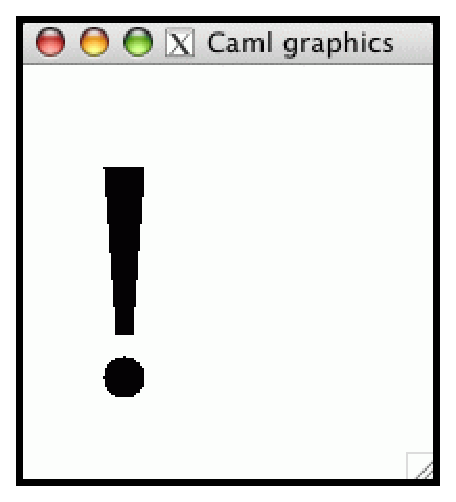
\includegraphics[scale=0.3]{graphics1}
\end{tabular}
\end{center}
%
\index{objects!dynamic lookup}
%
This example illustrates a property of object-oriented programming called \emph{dynamic lookup}.
%
\footnote{Dynamic lookup is often called \emph{polymorphism} in object-oriented circles, but that
  conflicts with the term \emph{polymorphism} that we use for ML.  The two are not at all the same.
  Following Mitchell~\cite{Mit03}, we'll use the term polymorphism to refer to \emph{parametric
    polymorphism} (type polymorphism), and \emph{dynamic lookup} to refer to object polymorphism.}
%
For an expression \hbox{\lstinline/obj#m/}, the actual method \hbox{\lstinline/m/} that gets called is determined
dynamically by the object \hbox{\lstinline/obj/}, not by some static property of the program.  A polygon
draws itself one way, a circle draws itself in another way, but the implementation is the
responsibility of the object, not the client.

\section{Encapsulation and polymorphism}
\label{section:object-constraint}
\index{row polymorphism}
\index{objects!encapsulation}

Another important feature of object-oriented programming is \emph{encapsulation}, also
called \emph{abstraction}.  An object encapsulates some data with methods for operating on the data;
it isn't necessary to know how an object is implemented in order to use it.  In our example, the
polygon and the circle have a single method \hbox{\lstinline/draw/}, so they have the same type, and they
can be used in the same ways.  Let's define a function to draw a list of objects.

\begin{ocaml}
# let draw_list items =
     List.iter (fun item -> item#draw) items;;
@
\begin{topoutput}
val draw_list : < draw : unit; .. > list -> unit = <fun>
\end{topoutput}
@
# draw_list [poly; circle];;
@
\begin{topoutput}
- : unit = ()
\end{topoutput}
@
\end{ocaml}
%
\index{row variables}
\index{row polymorphism}
\index{..@\lstinline/../ (in an object type)}
\label{keyword:..}
Note the type of the function \hbox{\lstinline/draw_list/}, which specifies that it takes a list of objects
of type \hbox{\lstinline/< draw : unit; .. >/}.  The ellipsis \hbox{\lstinline/../} in this type stands for ``other''
methods.  That is, the function \hbox{\lstinline/draw_list/} takes a list of objects having at least a
method \hbox{\lstinline/draw : unit/}, and possibly some other methods.  Suppose we defined a new kind of
object that represents a square that, in addition to having a method \hbox{\lstinline/draw/}, also defines
a method \hbox{\lstinline/area/} to compute the area.

\begin{center}
\begin{tabular}{cc}
\begin{minipage}[b]{3in}
\begin{ocamllistingx}
# let square =
  object
     val lower_left = (100, 100)
     val width = 10
     method area = width * width
     method draw =
        let (x, y) = lower_left in
        Graphics.fill_rect x y width width
  end;;
@
\begin{topoutput}
val square : < area : int; draw : unit > = <obj>
\end{topoutput}
@
# draw_list [square];;
@
\begin{topoutput}
- : unit = ()
\end{topoutput}
@
\end{ocamllistingx}
\end{minipage}
&
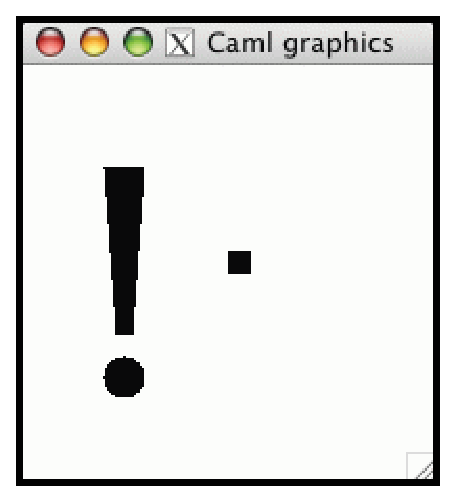
\includegraphics[scale=0.3]{graphics1a}
\end{tabular}
\end{center}
%
If we had used the simpler type \hbox{\lstinline/draw_list_exact : < draw : unit > list -> unit/}, the list
drawing function would work only with objects having \emph{exactly one} method, the
method \hbox{\lstinline/draw/}.  The expression \hbox{\lstinline/draw_list_exact [square]/} produces a type error,
because the object \hbox{\lstinline/square/} has an extra method \hbox{\lstinline/area/}.

\begin{ocaml}
# let draw_list_exact (items : < draw : unit > list) =
     List.iter (fun item -> item#draw) items;;
@
\begin{topoutput}
val draw_list_exact : < draw : unit > list -> unit = <fun>
\end{topoutput}
@
# draw_list_exact [square];;
@
\begin{toperror}
Characters 17-23:
  draw_list_exact [square];;
                   ^^^^^^
This expression has type < area : int; draw : unit >
but is here used with type < draw : unit >
The second object type has no method area
\end{toperror}
@
\end{ocaml}
%
Technically speaking, an occurrence of an ellipsis \hbox{\lstinline/../} in an object type is called a \emph{row
variable}, and the scheme for typing is called \emph{row polymorphism}.  It might not look like it,
but the type is really polymorphic, as we'll see if we try to write a type definition.

\begin{ocaml}
# type blob = < draw : unit; ..>;;
@
\begin{toperror}
Characters 4-30:
  type blob = < draw : unit; ..>;;
      ^^^^^^^^^^^^^^^^^^^^^^^^^^
A type variable is unbound in this type declaration.
In definition < draw : unit; .. > as 'a the variable 'a is unbound
\end{toperror}
@
\end{ocaml}
%
\label{keyword:as(object-types)}
\label{keyword:constraint}
\index{as!in object types}
\index{constraint@\lstinline/constraint/ (in object types)}
The issue is that an ellipsis \hbox{\lstinline/../} is like a type variable, standing for the types of all the
``other'' methods.  Unfortunately, it doesn't look like a type variable, and it doesn't make sense to
write \hbox{\lstinline/type (..) blob = < draw : unit; .. >/}.  The error message is a little cryptic, but
it suggests the solution, which is to introduce a type variable \hbox{\lstinline/'a/} that stands for the
type of the entire object.  The \hbox{\lstinline/as/} form and the \hbox{\lstinline/constraint/} form are
equivalent; you can write it either way.

\begin{ocaml}
# type 'a blob = < draw : unit; .. > as 'a;;
@
\begin{topoutput}
type 'a blob = 'a constraint 'a = < draw : unit; .. >
\end{topoutput}
@
# let draw_list_poly : 'a blob list -> unit = draw_list;;
@
\begin{topoutput}
val draw_list_poly : < draw : unit; .. > blob list -> unit = <fun>
\end{topoutput}
@
# draw_list_poly [square];;
@
\begin{topoutput}
- : unit = ()
\end{topoutput}
@
\end{ocaml}

\labelsection{objects-functional-update}{Transformations}

\index{transformation matrices}
%
An important feature of any 2D graphics library is the ability to transform objects by scaling,
rotation, or translation.  The cleanest way to do this is to make use of so-called \emph{homogeneous
  coordinates}, where the 2D coordinates $(x, y)$ are represented as triples $(x, y, 1)$, and
transformations are represented as $3{\times}3$ \emph{transformation matrices}.  A $3{\times}3$
matrix has 9 values $t_{ij}$, written as follows.

$$
\left(
\begin{array}{ccc}
t_{11} & t_{12} & t_{13}\\
t_{21} & t_{22} & t_{23}\\
t_{31} & t_{32} & t_{33}
\end{array}
\right)
$$
%
The product of a matrix and a vector is computed as follows, where $a b$ represents the product
of $a$ and $b$.

$$
\begin{array}{l}
\left(
\begin{array}{ccc}
t_{11} & t_{12} & t_{13}\\
t_{21} & t_{22} & t_{23}\\
t_{31} & t_{32} & t_{33}
\end{array}
\right)

\left(
\begin{array}{c}
x\\
y\\
z
\end{array}
\right)

=

\left(
\begin{array}{c}
t_{11} x + t_{12} y + t_{13} z\\
t_{21} x + t_{22} y + t_{23} z\\
t_{33} x + t_{23} y + t_{33} z
\end{array}
\right)
\end{array}
$$
%
The product of two matrices is computed as follows,

$$
\begin{array}{l}
\left(
\begin{array}{ccc}
s_{11} & s_{12} & s_{13}\\
s_{21} & s_{22} & s_{23}\\
s_{31} & s_{32} & s_{33}
\end{array}
\right)

\left(
\begin{array}{ccc}
t_{11} & t_{12} & t_{13}\\
t_{21} & t_{22} & t_{23}\\
t_{31} & t_{32} & t_{33}
\end{array}
\right)

=

\left(
\begin{array}{ccc}
u_{11} & u_{12} & u_{13}\\
u_{21} & u_{22} & u_{23}\\
u_{31} & u_{32} & u_{33}
\end{array}
\right)
\end{array}
$$
%
where $u_{ij} = s_{i1} t_{1j} + s_{i2} t_{2j} + s_{i3} t_{3j}$.

\subsection{Basis transformations}

The basis transformation matrices are specified as follows.
$$
\begin{array}{ccc}
\hbox{Scale by $(s_x, s_y)$} & \hbox{Rotate by $\theta$} & \hbox{Translate by $(\ms{dx}, \ms{dy})$}\\
\hline
\left(
\begin{array}{ccc}
s_x & 0 & 0\\
0 & s_y & 0\\
0 & 0 & 1
\end{array}
\right)
&
\left(
\begin{array}{ccc}
\cos \theta & -\sin \theta & 0\\
\sin \theta & \cos \theta & 0\\
0 & 0 & 1
\end{array}
\right)
&
\left(
\begin{array}{ccc}
1 & 0 & \ms{dx}\\
0 & 1 & \ms{dy}\\
0 & 0 & 1
\end{array}
\right)
\end{array}
$$
%
Transformations are composed by multiplying their matrices.  The application of a transformation to
a point is also a matrix multiplication, treating the coordinate as a column vector.  The following
formula represents a scaling by $(s_x, s_y)$ followed by a translation by $(\ms{dx}, \ms{dy})$ (for a
formula $(T_n \cdots T_2 T_1) p$, the matrix $T_1$ is the first transformation, and $T_n$ is the
last).

$$
\begin{array}{cl}
&
\left(
\left(
\begin{array}{ccc}
1 & 0 & \ms{dx}\\
0 & 1 & \ms{dy}\\
0 & 0 & 1
\end{array}
\right)
\times
\left(
\begin{array}{ccc}
s_x & 0 & 0\\
0 & s_y & 0\\
0 & 0 & 1
\end{array}
\right)
\right)
\times
\left(
\begin{array}{c}
x\\
y\\
1
\end{array}
\right)
\\
\\
= &
\left(
\begin{array}{ccc}
s_x & 0 & \ms{dx}\\
0 & s_y & \ms{dy}\\
0 & 0 & 1
\end{array}
\right)
\times
\left(
\begin{array}{c}
x\\
y\\
1
\end{array}
\right)
=
\left(
\begin{array}{c}
s_x x + \ms{dx}\\
s_y y + \ms{dy}\\
1
\end{array}
\right)
\end{array}
$$
%
\subsection{Functional update}

Let's implement an object that represents a transformation matrix.  We could implement three
separate functions to produce the basis transformations, but that would require duplicating the
object definition.  It will be easier to implement them as methods instead.

Let's start with the basis transformations.  Since the last row in a transformation is always $(0\ 0\
1)$, we'll just omit it and use a flattened 6-tuple to represent the matrix.

$$
\begin{array}{ccc}
\hbox{Matrix} & & \hbox{Flattened representation as a 6-tuple}\\
\hline
\left(
\begin{array}{ccc}
x_{11} & x_{12} & x_{13}\\
x_{21} & x_{22} & x_{23}\\
0 & 0 & 1
\end{array}
\right)
&
\Longrightarrow
&
(x_{11}, x_{12}, x_{13}, x_{21}, x_{22}, x_{23})
\end{array}
$$
%
First, let's write the methods \hbox{\lstinline/new_scale/}, \hbox{\lstinline/new_rotate/},
and \hbox{\lstinline/new_translate/} that construct the basis transformations.  For the moment, we're
omitting the implementations of the methods \hbox{\lstinline/transform/} and \hbox{\lstinline/multiply/}.

\begin{ocaml}
# let transform =
object
   val matrix = (1., 0., 0., 0., 1., 0.)
   method new_scale sx sy =
      {< matrix = (sx, 0., 0., 0., sy, 0.) >}
   method new_rotate theta =
      let s, c = sin theta, cos theta in
      {< matrix = (c, -.s, 0., s, c, 0.) >}
   method new_translate dx dy =
      {< matrix = (1., 0., dx, 0., 1., dy) >}
   method transform (x, y) = $\cdots$
   method multiply matrix2 = $\cdots$
end;;
@
\begin{topoutput}
val transform :
  < new_scale : float -> float -> 'a;
    new_rotate : float -> 'a;
    new_translate : float -> float -> 'a;
    transform : float * float -> int * int;
    multiply : ... > as 'a = <obj>
\end{topoutput}
@
\end{ocaml}
%
\label{keyword:functional-object-update}
\index{objects!functional update}
The expression \hbox{\lstinline/{< $\cdots$ >}/} represents a \emph{functional update}.  This kind
of update produces a new object that is the same as the current object, except for the specified
changes; the original object is not affected.  For example, an expression \hbox{\lstinline/{< >}/} would
produce an identical copy of the current object.  In the \hbox{\lstinline/transform/} object, the
expression \hbox{\lstinline/{< matrix = $\nt{expression}$ >}/} produces a new transform object with new
values for the field \hbox{\lstinline/matrix/}.  In our example, the canonical object \hbox{\lstinline/transform/}
is the identity transformation, and each basis method \hbox{\lstinline/new_$\ldots$/} produces a new object
by discarding the original value of the field \hbox{\lstinline/matrix/}, and replacing it with new values
that implement the desired transformation.  In effect, each method \hbox{\lstinline/new_$\ldots$/} is
a \emph{constructor} that constructs a new object, using the current one as a template.

In general, there are two things to keep in mind when using a functional update.  First, the
expression form \hbox{\lstinline/{< $\cdots$ >}/} can be used only in a method body.  Second, the update
can be used only to update fields, not methods---method implementations are fixed at the time the
object is created.

\section{Binary methods}

Let's return to the implementation and fill in the remaining methods.  The
method \hbox{\lstinline/transform/} is just a matrix multiplication, which we write out by hand.

\label{page:transform-methods}
\begin{ocaml}
   method transform (x, y) =
      let (m11, m12, m13, m21, m22, m23) = matrix in
      (m11 *. x +. m12 *. y +. m13,
       m21 *. x +. m22 *. y +. m23)
\end{ocaml}
%
\index{objects!binary methods}
The \hbox{\lstinline/multiply/} method is a little harder.  The problem is that in OCaml, unlike some other
object-oriented languages, fields are private to an object.  The \hbox{\lstinline/multiply/} method is
called a \emph{binary method} because it takes another object of the same type as an argument.  A
binary method cannot directly access the fields of the object passed as an argument.

\label{objects:binary-methods}
There are several approaches to dealing with binary methods, but the easiest one here is to add a
method \hbox{\lstinline/representation/} that exposes the internal representation of the object.\footnote{Of
course, this is not always desirable.  In Section~\ref{section:modules-classes}, we describe a way
to use the module system to improve abstraction.}  The remaining part of the implementation is as
follows.

\begin{ocaml}
# let transform =
object
   $\cdots$
   method representation = matrix
   method multiply matrix2 =
      let (x11, x12, x13, x21, x22, x23) = matrix in
      let (y11, y12, y13, y21, y22, y23) = matrix2#representation in
      {< matrix =
            (x11 *. y11 +. x12 *. y21,
             x11 *. y12 +. x12 *. y22,
             x11 *. y13 +. x12 *. y23 +. x13,
             x21 *. y11 +. x22 *. y21,
             x21 *. y12 +. x22 *. y22,
             x21 *. y13 +. x22 *. y23 +. x23)
      >}
end;;
@
\begin{topoutput}
val transform : < ... > as 'a = <obj>
\end{topoutput}
@
# let ( ** ) t1 t2 = t1#multiply t2;;
@
\begin{topoutput}
val ( ** ) : < multiply : 'a -> 'b; .. > -> 'a -> 'b = <fun>
\end{topoutput}
@
\end{ocaml}
%
\labelsection{objects-factories}{Object factories}

Now that we have defined the transformation, let's return to the graphical objects, where we now
want to add a new method \hbox{\lstinline/transform/} to apply a transformation to the object.  It can get
tedious to define an entire object each time it is created, so instead we will write functions that
create new objects (functions that create new objects are often called \emph{factories}).  In
addition, we now represent the coordinates as pairs of floating-point numbers.  Here is the
implementation of the factory \hbox{\lstinline/new_poly/}; the code for circles is similar.\footnote{Note
that the function to draw circles \hbox{\lstinline/Graphics.fill_circle/} takes the circle's radius.  In
general, however, a transformed circle should be an ellipse.}

\begin{ocaml}
# let int_coord (x, y) = (int_of_float x, int_of_float y);;
@
\begin{topoutput}
val int_coord : float * float -> int * int = <fun>
\end{topoutput}
@
# let new_poly vertices =
object
   val vertices = vertices
   method draw = Graphics.fill_poly (Array.map int_coord vertices)
   method transform matrix = {< vertices = Array.map matrix#transform vertices >}
end;;
@
\begin{topoutput}
val new_poly :
  (float * float) array ->
  (< draw : unit;
     transform : < transform : float * float -> float * float; .. > -> 'a >
   as 'a) = <fun>
\end{topoutput}
@
\end{ocaml}
%
Note the type of the \hbox{\lstinline/transform/} method, which is more subtle than it might seem.
Remember that the ellipsis \hbox{\lstinline/../} is a row variable---it is like a type variable, so
the type of polygons really contains two type variables.  We'll revisit this issue in the next
section.

Finally, to illustrate our graphics library in action, let's draw a few transformed and rotated
objects.

\begin{ocaml}
let poly = new_poly [|(-0.05, 0.2); (0.05, 0.2); (0.1, 1.0); (-0.1, 1.0)|] in
let circle = new_circle (0.0, 0.0) 0.1 in
let matrix1 =
   (transform#new_translate 50.0 50.0) ** (transform#new_scale 100.0 100.0) in
   for i = 0 to 9 do
      let matrix2 = matrix1 ** (transform#new_rotate (0.628 *. float_of_int i)) in
      (poly#transform matrix2)#draw
   done;
   (circle#transform matrix1)#draw;;
\end{ocaml}
%
This program starts with two objects, \hbox{\lstinline/poly/} and \hbox{\lstinline/circle/}, centered at the
origin.  The initial transformation \hbox{\lstinline/matrix1/} scales by 100 and centers the image on $(50,
50)$.  The transformation \hbox{\lstinline/matrix2/} draws a ray rotated about the point $(50, 50)$ to form a
kind of star.  The following image shows the output.

\centerline{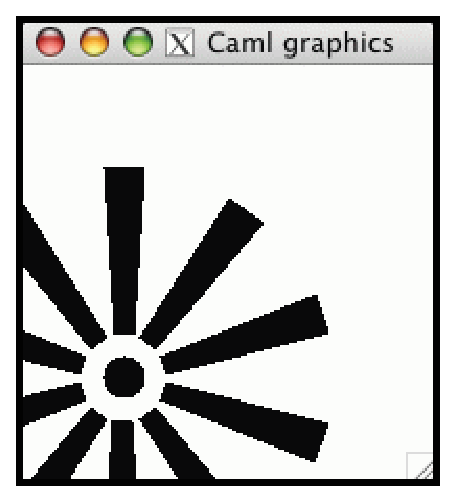
\includegraphics[scale=0.3]{graphics2}}

\section{Imperative objects}

\label{keyword:mutable(objects)}
\index{objects!imperative}
\index{mutable!object fields}
Next, it is natural to want to define a collection of items that acts like a single drawable object.
This time, let's define it imperatively, so that the collection includes a method \hbox{\lstinline/add/}
that adds an item to the collection by side-effect.  The syntax for a field that can be modified is
\hbox{\lstinline/val mutable $\nt{identifier}$ = $\nt{expression}$/}.

\label{keyword:<-(object-field-assignment)}
\index{<-!object field assignment}
\index{objects!mutable fields}
\begin{ocaml}
# let new_collection () =
object
   val mutable items = []
   method add item = items <- item :: items
   method draw = List.iter (fun item -> item#draw) items
   method transform matrix =
      {< items = List.map (fun item -> item#transform matrix) items >}
end;;
@
\begin{topoutput}
val new_collection :
  unit ->
  (< add : (< draw : unit; transform : 'c -> 'b; .. > as 'b) -> unit;
     draw : unit; transform : 'c -> 'a >
   as 'a) = <fun>
\end{topoutput}
@
\end{ocaml}
%
Apart from the inferred type, the definition is reasonably simple.  The field \hbox{\lstinline/items/} is
declared as mutable, and the method \hbox{\lstinline/add/} modifies it by side-effect (using \hbox{\lstinline/<-/}
for assignment).  Let's build a star.

\begin{ocaml}
let star =
   let poly = new_poly [|(0.0, 0.2); (0.1, 0.5); (0.0, 1.0); (-0.1, 0.5)|] in
   let star = new_collection () in
   star#add (new_circle (0.0, 0.0) 0.1);
   for i = 0 to 9 do
      let trans = transform#new_rotate (0.628 *. (float_of_int i)) in
      star#add (poly#transform trans)
   done;
   star;;
\end{ocaml}
%
Since the \hbox{\lstinline/star/} object is also a drawable object, we can also build a collection with
multiple stars.

\begin{ocaml}
let starry_night =
   let starry_night = new_collection () in
   let add_star (x, y, scale) =
      let trans = (transform#new_translate x y)
         ** (transform#new_scale scale scale) in
      starry_night#add (star#transform trans) in
   List.iter add_star
      [0.35, 0.50, 0.15;
       0.12, 0.95, 0.12;
       0.35, 0.95, 0.10;
       0.62, 0.90, 0.12;
       0.95, 0.85, 0.20];
   starry_night
\end{ocaml}
%
The images for the objects \hbox{\lstinline/star/} and \hbox{\lstinline/starry_night/} are shown below.

\begin{center}
\begin{tabular}{cc}
\hbox{\lstinline/star/} & \hbox{\lstinline/starry_night/}\\
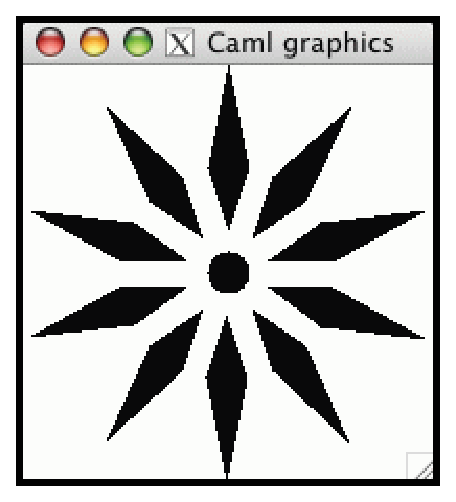
\includegraphics[scale=0.3]{graphics3}
&
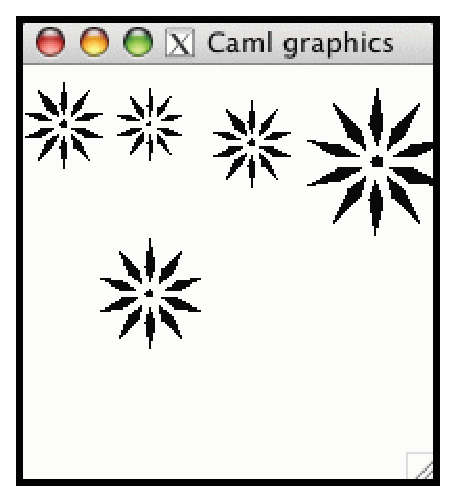
\includegraphics[scale=0.3]{graphics4}
\end{tabular}
\end{center}

\section{self: referring to the current object}

\label{objects:self}
\label{keyword:hash}
\index{self@\lstinline/self/}
\index{objects!self (the current object)}
Suppose we wish to define a method that is recursive, or a method that calls another method in the same
object.  In OCaml, the fields of an object can be referred to directly by name, but methods must
always use the syntax \hbox{\lstinline/$\nt{object}$#$\nt{method-name}$/}.  If we wish to call a method in
the current object, the object must first be named with the following syntax, where the name occurs in
parenthesis after the \hbox{\lstinline/object/} keyword.

\begin{ocaml}
object ($\nt{pattern}$) $\cdots$ end
\end{ocaml}
%
The pattern can use any identifier, but by convention the current object is usually
named \hbox{\lstinline/self/}.  It is often specified with a type as well.  The following form is conventional,
where the name \hbox{\lstinline/self/} refers to the current object, and \hbox{\lstinline/'self/} is its type.

\begin{ocaml}
object (self : 'self) $\cdots$ end
\end{ocaml}
%
Now that we have a name for the current object, let's define a collection method
\hbox{\lstinline/add_multiple n trans item/} that adds \hbox{\lstinline/n/} of the \hbox{\lstinline/item/}
to the collection, transforming each copy.  The easiest way to define the method is to make it
recursive.

\begin{ocaml}
let new_collection () =
   object (self : 'self)
      val mutable items = []
      method add item = items <- item :: items
      method add_multiple n matrix item =
         if n > 0 then begin
            self#add item;
            self#add_multiple (n - 1) matrix (item#transform matrix)
         end
      method draw = List.iter (fun item -> item#draw) items
      method transform matrix = $\cdots$
   end;;
\end{ocaml}
%
The expression \hbox{\lstinline/self#add item/} is a method call that adds the item to the current
collection, and \hbox{\lstinline/self#add_multiple/} is a recursive call.

\begin{center}
\begin{tabular}{cc}
\begin{minipage}[b]{3.5in}
\begin{ocamllisting}
let line =
   new_poly [|(0., 0.); (2., 0.); (2., 30.); (0., 30.)|];;
let xform =
   transform#new_translate 3. 0. ** transform#new_scale 1.1 1.1;;
let image = new_collection ();;
image#add_multiple 25 xform line;;
image#draw;;
\end{ocamllisting}
\end{minipage}
&
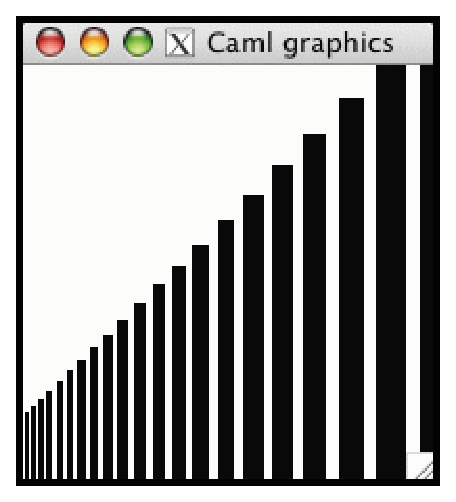
\includegraphics[scale=0.3]{graphics8}
\end{tabular}
\end{center}

\section{Initializers; private methods}

There is an important rule to keep in mind when constructing objects.

\begin{center}
---Field expressions may not refer to other fields, nor to \emph{self}.---
\end{center}
%
Here is an example.

\begin{ocaml}
# object
     val x = 1
     val x_plus_1 = x + 1
  end;;
@
\begin{topoutput}
Characters 38-39:
     val x_plus_1 = x + 1
                    ^
The instance variable x
cannot be accessed from the definition of another instance variable
\end{topoutput}
@
\end{ocaml}
%
The technical reason for this is that the object doesn't exist when the field values are being
computed, so it is an error to refer to the object or any of its fields and methods.

\label{keyword:initializer}
As one way of addressing this problem, objects can contain an \emph{initializer}, written
\hbox{\lstinline/initializer $\nt{expression}$/}.
The initializer expression is evaluated just after the object is created, but before it is used.  The
object exists at initialization, so it is legal to refer to its fields and methods in the
initializer.

\begin{ocaml}
# object
     val x = 1
     val mutable x_plus_1 = 0
     initializer
        x_plus_1 <- x + 1
  end;;
\end{ocaml}
%
Initializers are especially useful when an object has an invariant to be maintained, or when the
value of one field is derived from another.  For a more realistic example along these lines, let's
write a version of the polygon object that allows the polygon to be transformed in place (by
side-effect).

\begin{ocaml}
let new_imp_poly vertices =
   object
      val mutable vertices = vertices
      method draw = Graphics.fill_poly (Array.map int_coord vertices)
      method transform matrix = {< >}#transform_in_place matrix
      method transform_in_place matrix =
         vertices <- Array.map matrix#transform vertices
   end;;
\end{ocaml}
%
One potential source of inefficiency in this object is that the vertices are represented with floating-point coordinates, but must be drawn with integer coordinates.  The method \hbox{\lstinline/draw/} performs the conversion each time the object is drawn.

An alternative is to maintain two versions of the vertices, \hbox{\lstinline/float_vertices/}
and \hbox{\lstinline/int_vertices/}, with the invariant that
\hbox{\lstinline/int_vertices = Array.map int_coord float_vertices/}.
When one field is derived from another like this, it is usually best to define a method that handles
changes to the fields.  In this case, the method \hbox{\lstinline/set_vertices/} updates the object with
new coordinates.

\begin{ocaml}
# let new_imp_poly vertices =
object (self : 'self)
   val mutable float_vertices = [||]
   val mutable int_vertices = [||]
   method draw = Graphics.fill_poly int_vertices
   method transform matrix = {< >}#transform_in_place matrix
   method transform_in_place matrix =
      self#set_vertices (Array.map matrix#transform vertices)
   method private set_vertices vertices =
      float_vertices <- vertices;
      int_vertices <- Array.map int_coord float_vertices
   initializer
      self#set_vertices vertices
end;;
@
\begin{topoutput}
val new_imp_poly : (float * float) array ->
  < draw : unit;
    transform : (< transform : float * float -> float * float; .. > as 'a) -> unit;
    transform_in_place : 'a -> unit > = <fun>
\end{topoutput}
@
\end{ocaml}
%
The method \hbox{\lstinline/set_vertices/} is called in two places, 1) by the \hbox{\lstinline/initializer/} to set
the initial values of the vertices, and 2) by the method \hbox{\lstinline/transform_in_place/}, which
computes new values for the vertices.  The object reference \hbox{\lstinline/self/} is legal in the
initializer, allowing the method call \hbox{\lstinline/self#set_vertices/}.

\label{keyword:private}
This example also contains a \emph{private method}.  Private methods are defined with the syntax
\hbox{\lstinline/method private $\nt{identifier}$ = $\nt{expression}$/}.
They are used just like normal (public) methods, but they are not visible outside the object---they
don't even appear in the object type.

\section{Object types, coercions, and subtyping}

The types of the objects we have been creating are getting pretty complicated.
To make sense of it all, let's make some type definitions.  We don't really care about
giving the most general polymorphic types, so let's use exact non-polymorphic types instead.  We'll
call a drawable object a \hbox{\lstinline/blob/}.

\begin{ocaml}
type coord = float * float
type transform = < transform : coord -> coord >
type blob = < draw : unit; transform : transform -> blob >
type collection =
   < add : blob -> unit;
     draw : unit;
     transform : transform -> collection
   >
\end{ocaml}
%
Note that the type \hbox{\lstinline/collection/} differs from \hbox{\lstinline/blob/} in two ways.  A collection
has an extra method \hbox{\lstinline/add/}, and the method \hbox{\lstinline/transform/} returns another
collection, not a blob.

We can now annotate the object creation functions to get simpler types (the object definitions are
the same as before).

\begin{ocaml}
# let new_poly (vertices : coord array) : blob = object $\cdots$ end;;
@
\begin{topoutput}
val new_poly : coord array -> blob = <fun>
\end{topoutput}
@
# let new_circle (center : coord) radius : blob = object $\cdots$ end;;
@
\begin{topoutput}
val new_circle : coord -> float -> blob = <fun>
\end{topoutput}
@
# let new_collection () : collection = object $\cdots$ end;;
@
\begin{topoutput}
val new_collection : unit -> collection = <fun>
\end{topoutput}
@
\end{ocaml}
%
Now that the types are simplified, we run into a new issue: the actual object types do not match the
expected exact types.  For example, the method \hbox{\lstinline/transform/} now expects an object with
exactly one method (the method is also called \hbox{\lstinline/transform/}), but the real object has many more methods.
Here is what we get if we try to perform a transformation.

\begin{ocaml}
# let circle = new_circle (0.0, 0.0) 0.1;;
@
\begin{topoutput}
val circle : blob = <obj>
\end{topoutput}
@
# circle#transform (transform#new_translate 100.0 100.0);;
@
\begin{topoutput}
Characters 17-54:
  circle#transform (transform#new_translate 100.0 100.0);;
                   ^^^^^^^^^^^^^^^^^^^^^^^^^^^^^^^^^^^^^
This expression has type
  < multiply : ... > as 'a
but is here used with type transform
The second object type has no method multiply
\end{topoutput}
@
\end{ocaml}
%
The problem here is that the expression \hbox{\lstinline/(transform#new_translate 100.0 100.0)/} produces
an actual object with many methods, while the method \hbox{\lstinline/circle#transform/} expects an object
having exactly one method.  In principle, it should be fine to pass an object with more methods to
one that expects fewer---all the extra methods can simply be ignored.

\subsection{Coercions}

\label{keyword::>}
\index{objects!coercions}
\index{:>@\lstinline/:>/ object coercion}
In OCaml, such coercions are in fact legal, but they are not automatic.  This is in accord with the usual
OCaml policy that all coercions should be explicit; for example, integers are never coerced automatically
to floating-point values, the function \hbox{\lstinline/float_of_int/} must be written explicitly.

An explicit object coercion can be written two ways, as a ``single coercion'' or as a ``double coercion.''

\begin{center}
\begin{tabular}{ll}
    \lstinline/($\nt{object}$ :> $\nt{object-type}$)/ & single coercion\\
    \lstinline/($\nt{object}$ : $\nt{object-type}$ :> $\nt{object-type}$)/ & double coercion
\end{tabular}
\end{center}
%
The single coercion expression \hbox{\lstinline/($e$ :> $t$)/} coerces the object $e$ to have type $t$ (if
legal).  The double coercion expression \hbox{\lstinline/($e$ : $t_1$ :> $t_2$)/} means to consider first
that $e$ has type $t_1$, then coerce it to an object of type $t_2$.  In most cases, a single
coercion is sufficient.

\begin{ocaml}
# circle#transform (transform#new_translate 100.0 100.0 :> transform);;
@
\begin{topoutput}
- : blob = <obj>
\end{topoutput}
@
\end{ocaml}
%
For another example, consider the collection object, which contains a list of simple blobs.
If we want to add any other kind of object, it must be coerced.

\begin{ocaml}
# let image = new_collection ();;
@
\begin{topoutput}
val image : collection = <obj>
\end{topoutput}
@
# image#add (new_circle (0.0, 0.0) 0.1);;
@
\begin{topoutput}
- : unit = ()
\end{topoutput}
@
# image#add star;;
@
\begin{toperror}
Characters 10-14:
  image#add star;;
            ^^^^
This expression has type collection but is here used with type blob
The second object type has no method add
\end{toperror}
@
\end{ocaml}
%
That is as we expected, but the single coercion doesn't work either.

\begin{ocaml}
# image#add (star :> blob);;
@
\begin{topoutput}
Characters 11-15:
  image#add (star :> blob);;
             ^^^^
This expression cannot be coerced to type
  blob = < draw : unit; transform : transform -> blob >;
...
This simple coercion was not fully general. Consider using a double coercion.
\end{topoutput}
@
\end{ocaml}
%
The real error message is quite long, most of it has been elided.  The last line suggests using a
double coercion, so we try that.  Finally, success.

\begin{ocaml}
# star;;
@
\begin{topoutput}
- : collection = <obj>
\end{topoutput}
@
# image#add (star : collection :> blob);;
@
\begin{topoutput}
- : unit = ()
\end{topoutput}
@
\end{ocaml}
%
\index{coercions (single \emph{vs}.{} double)}
%
Why does the single coercion sometimes work, but at other times the double coercion is required?
The complete technical explanation is complicated and has to do with the specific algorithm used for
type inference.  The simplest rule is this: if the compiler complains about a single coercion, try
replacing it with a double coercion.  If you would like to know the real reason, a bit of
explanation might be helpful.

Internally, the compiler uses only double coercions.  Whenever the compiler encounters a single
coercion \hbox{\lstinline/($e$ :> $t_2$)/} it constructs a double coercion
%
\hbox{\lstinline/($e$ : $t_1$ :> $t_2$)/} by inferring the \emph{most general expected type} $t_1$.
However, this fails if there is no unique most general expected type.  The general guidelines can be
stated as follows.
%
\begin{quote}
A single coercion \hbox{\lstinline/($e$ :> $t_2$)/} may fail if:
\begin{itemize}
\item the type $t_2$ is recursive, or
\item the type $t_2$ has polymorphic structure.
\end{itemize}
If either condition holds, use a double coercion \hbox{\lstinline/($e$ : $t_1$ :> $t_2$)/}.
\end{quote}
%
In our example, the single coercion \lstinline/(transform#new_translate 100.0 100.0 :> transform)/
is successful because the type \hbox{\lstinline/transform/} is neither recursive nor polymorphic.  However,
the coercion \hbox{\lstinline/(star :> blob)/} fails because the type \hbox{\lstinline/blob/} is recursive.  The
compiler doesn't consider the actual type of the expression, so even though we know
\hbox{\lstinline/star/} has type \hbox{\lstinline/collection/}, it is still necessary to write the double coercion
\hbox{\lstinline/(star : collection :> blob)/}.  

\labelsubsection{subtyping}{Subtyping}

\index{objects!subtyping}
\index{subtyping!relation}
\index{<:@$\subtype$ relation}
That's not the entire story of course, because not all coercions \hbox{\lstinline/($e$ : $t_1$ :> $t_2$)/}
are legal.  There are two necessary conditions: first, expression $e$ should have type $t_1$; and
second, type $t_1$ must be a subtype of $t_2$.

We say that a type $t_1$ is a \emph{subtype} of $t_2$, written $t_1 \subtype t_2$, if values of type
$t_1$ can be used where values of type $t_2$ are expected.  It may be confusing that the
symbols \hbox{\lstinline$:>$} (the coercion operator) and $\subtype$ (the
subtyping relation) look like they point in opposite directions.  It may be
helpful to remember that the former is an operator, and the latter is
a relation not belonging to the syntax of the language.

Consider the following type definitions: an \hbox{\lstinline/animal/} eats, and a \hbox{\lstinline/dog/} also
barks.

\begin{ocaml}
type animal = < eat : unit >
type dog = < eat : unit; bark : unit >
\end{ocaml}
%
The subtyping relation $\mt{dog} \subtype \mt{animal}$ holds because a \hbox{\lstinline$dog$} object
has all the methods that an animal has with the same type, and so a dog object $e$ can be used wherever
an \hbox{\lstinline$animal$} object is expected (so the coercion \hbox{\lstinline/($e$ : dog :> animal)/} is legal).

\subsubsection{Width and depth subtyping}
\label{section:width-subtyping}

\index{subtyping!width}
\index{subtyping!depth}
Subtyping for object types takes two forms, called \emph{width} and \emph{depth} subtyping.  Width
subtyping means that an object type $t_1$ is a subtype of object type $t_2$ if $t_1$ implements all
the methods (and possibly more) of $t_2$ with the same method types.  The order of methods in an
object type doesn't matter, so we can write this as follows, where we use the
notation \hbox{\lstinline/$f_{1..n}$ : $t_{1..n}$/} to represent $n$ method
declarations \hbox{\lstinline/$f_i$ : $t_i$/} for $i \in \{ 1, 2, \ldots, n \}$.

\begin{ocaml}
< $f_{1..n}$ : $t_{1..n}$, $g_{1..m}$ : $s_{1..m}$ > $\subtype$ < $f_{1..n}$ : $t_{1..n}$ >
\end{ocaml}
%
The subtyping relation $\mt{dog} \subtype \mt{animal}$ follows from width subtyping, because class
type \hbox{\lstinline$dog$} implements the \hbox{\lstinline$eat$} method, the only method in
the \hbox{\lstinline$animal$} class type.

\begin{ocaml}
< eat : unit; bark : unit > $\subtype$ < eat : unit >
\end{ocaml}
%
Depth subtyping means that an object type $t_1$ is a subtype of
$t_2$ if the two types have the same methods, but the method
types in $t_1$ are subtypes of the corresponding types in
$t_2$.  This rule is usually written as follows, as an \emph{inference
rule}, where the subtyping properties above the horizontal line imply
the subtyping property below the line.  We read it informally as
follows, ``If each method type $s_i$ is a subtype of method type
$t_i$, then the object type \hbox{\lstinline/< $f_{1..n}$ : $s_{1..n}$ >/}
is a subtype of the object type \hbox{\lstinline/< $f_{1..n}$ : $t_{1..n}$ >/}.''

\begin{center}
\begin{tabular}{c}
$s_i \subtype t_i$ \quad (for each $i \in \{ 1, \ldots, n \}$)\\
\hline
\hbox{\lstinline/< $f_{1..n}$ : $s_{1..n}$ > $\subtype$ < $f_{1..n}$ : $t_{1..n}$ >/}
\end{tabular}
\end{center}
%
\index{covariant types}
\index{contravariant types}
\index{invariant types}
In general, the method types may include various type constructors for
tuples, lists, records, functions, other objects, \emph{etc}.  Each type
constructor in OCaml has its own subtyping rules describing how the
type construction varies in terms of its component types.  These
variances can be \emph{covariant}, meaning that the construction
varies in the same way as a component type; \emph{contravariant},
meaning the construction varies oppositely to a component type;
or \emph{invariant}, which means that it is neither purely covariant
nor purely contravariant.

For example, consider the tuple type \hbox{\lstinline/$t_1$ * $t_2$/}, which
is covariant in both types $t_1$ and $t_2$.  If we have two dogs
\hbox{\lstinline$dog * dog$}, then we also have two animals
\hbox{\lstinline$animal * animal$} (so 
\hbox{\lstinline/dog * dog $\subtype$ animal * animal/}).
The inference rule for pairs is specified as follows.

$$\infer{(s_1 * s_2) \subtype (t_1 * t_2)}{s_1 \subtype t_1 & s_2 \subtype s_2}$$

\subsubsection{Function subtyping}

\index{subtyping!function types}
Nearly all type constructors in OCaml are covariant over all their
component types, but there are two exceptions.  One is that types that specify
mutable values are always invariant.  The other exception is more
interesting, for the function type.  A function
type \hbox{\lstinline/$t_1$ -> $t_2$/} is covariant in its range type
$t_2$, but \emph{contravariant} in the domain type $t_1$.  This
property is written as follows.

$$\infer{(s_1 \mathrel{\mt{->}} s_2) \subtype (t_1 \mathrel{\mt{->}} t_2)}
{t_1 \subtype s_1 & s_2 \subtype t_2}$$
%
The contravariance in function types is the source of many problems in
the design of object-oriented programming languages, and it can be
difficult to understand.  To get some intuition, consider a
function \hbox{\lstinline$feed$} for feeding an animal.

\begin{ocaml}
# let feed (x : animal) = x#eat;;
@
\begin{topoutput}
val feed : animal -> unit = <fun>
\end{topoutput}
@
\end{ocaml}
%
When calling the function, we can pass it an \hbox{\lstinline$animal$} object
or a \hbox{\lstinline$dog$} object---both support the \hbox{\lstinline$eat$}
method.  Thus, if we like, we can coerce the function to have type
\hbox{\lstinline$dog -> unit$}.

\begin{ocaml}
# let feed_dog = (feed : animal -> unit :> dog -> unit);;
@
\begin{topoutput}
val feed_dog : dog -> unit = <fun>
\end{topoutput}
@
\end{ocaml}
%
Now consider an barking function for dogs.

\begin{ocaml}
# let do_bark (x : dog) = x#bark;;
@
\begin{topoutput}
val do_bark : dog -> unit = <fun>
\end{topoutput}
@
\end{ocaml}
%
We can't pass a plain \hbox{\lstinline$animal$} object
to \hbox{\lstinline$do_bark$}, because animals do not bark in general.  In
general, we \emph{cannot} use a function of type
\hbox{\lstinline$dog -> unit$} in places where a function of type
\hbox{\lstinline$animal -> unit$} is
expected.

\begin{ocaml}
# (do_bark : dog -> unit :> animal -> unit);;
@
\begin{toperror}
Characters 0-41:
  (do_bark : dog -> unit :> animal -> unit);;
  ^^^^^^^^^^^^^^^^^^^^^^^^^^^^^^^^^^^^^^^^^
Type dog -> unit is not a subtype of type animal -> unit 
Type animal = < eat : unit > is not a subtype of type
  dog = < bark : unit; eat : unit > 
\end{toperror}
@
\end{ocaml}

\subsubsection{Subtyping of recursive object types}

Finally, let's consider subtyping for recursive object types.  In this case, the subtyping rule is circular: first, assume that the subtyping relationship holds, then prove that it holds.  Don't worry---in this particular case the circular argument is sound.

For example, consider the argument that a \hbox{\lstinline/collection/} is a \hbox{\lstinline/blob/}.  The types
are recursive, so we first assume that the relation holds, and then prove it.  Here is the argument.

\begin{itemize}
\item Assume: \hbox{\lstinline/collection $\subtype$ blob/}.
\item Show:

\begin{tabular}{ccc}
\begin{minipage}{2in}
\begin{ocamllisting}
< add : blob -> unit;
  draw : unit;
  transform : transform -> collection
>
\end{ocamllisting}
\end{minipage}
&
$\subtype$
&
\begin{minipage}{2in}
\begin{ocamllisting}
< draw : unit;
  transform : transform -> blob
>
\end{ocamllisting}
\end{minipage}
\end{tabular}

\item From width subtyping, we can ignore the \hbox{\lstinline/add/} method.

\begin{tabular}{ccc}
\begin{minipage}{2in}
\begin{ocamllisting}
< draw : unit;
  transform : transform -> collection
>
\end{ocamllisting}
\end{minipage}
&
$\subtype$
&
\begin{minipage}{2in}
\begin{ocamllisting}
< draw : unit;
  transform : transform -> blob
>
\end{ocamllisting}
\end{minipage}
\end{tabular}

\item The \hbox{\lstinline/draw/} methods have the same type.
The \hbox{\lstinline/transform/} method is justified by depth subtyping.
We must show the following.

\begin{ocaml}
transform -> collection $\subtype$ transform -> blob
\end{ocaml}

\item Functions are covariant in the range type.  The final goal is the following.

\begin{ocaml}
collection $\subtype$ blob
\end{ocaml}

This follows by assumption.
\end{itemize}

\section{Narrowing}
\label{section:narrowing}

\index{subtyping!narrowing}
\index{narrowing}
In object-oriented programming, \emph{narrowing} is the ability to coerce an object to one of its
subtypes---the opposite of a normal coercion.  This is commonly used when the actual type of an
object has been lost due to a coercion somewhere else in the program.  For example, suppose we have
defined some types for cats and dogs.  If we want a list that contains both cats and dogs, the
elements of the list must coerced to a common type, in this case the supertype \hbox{\lstinline/animal/}.

\begin{ocaml}
type animal = < eat : unit >
type dog = < eat : unit; bark : unit >
type cat = < eat : unit; meow : unit >

let fido : dog = $\cdots$
let daphne : cat = $\cdots$

let animals = [(fido :> animal); (daphne :> animal)]
\end{ocaml}
%
Because of the coercion, the methods \hbox{\lstinline/bark/} and \hbox{\lstinline/meow/} have been lost, which can
be a potential problem.  Languages that support narrowing usually include a ``typecase'' to perform
a case analysis on an object's actual type.  The following function illustrates how a typecase
would be written, presented in OCaml-style pseudo-code.

\begin{ocaml}
(* THIS IS NOT LEGAL OCAML CODE *)
let chorus (animals : animal list) =
   List.iter (fun animal ->
      if @\textit{animal instanceof dog}@ then (animal :> dog)#bark
      else if @\textit{animal instanceof cat}@ then (animal :> cat)#meow) animals
\end{ocaml}
%
Narrowing is \textbf{not permitted} in OCaml.  Period.  First, we'll give some arguments why
narrowing is undesirable, then we'll describe how to do it anyway.

\subsection{Why narrowing is bad}

The usual argument against narrowing is that it is unsound.  Actually, it is probably more accurate
to say that it isn't known whether there is a useful, general form of narrowing that is compatible
with the OCaml type system.

We might leave it at that, but there are good \emph{design} principles that also argue against
narrowing.  One of the principal benefits of object-oriented programming is that the responsibility
of implementation is shifted to the object, away from the client.  The need for case analysis is
reduced because of dynamic lookup, which ensures that the code that is executed is always appropriate
to the object.

Looking at our example, the problem is that a single concept, let's call it ``\hbox{\lstinline/speak/},'' is named in two
different ways, \hbox{\lstinline/bark/} and \hbox{\lstinline/meow/}.  A better implementation would use the same
name in both cases, perhaps also keeping the species-specific name.

\begin{ocaml}
type animal = < eat : unit; speak : unit >
type dog = < eat : unit; speak : unit; bark : unit >
type cat = < eat : unit; speak : unit; meow : unit >
type lizard = < eat : unit; speak : unit; sleep : unit >
let fido : dog = object (self) method speak = self#bark $\cdots$ end
let daphne : cat = object (self) method speak = self#meow $\cdots$ end
let fred : lizard = object (self) method speak = () $\cdots$ end
let animals = [(fido :> animal); (daphne :> animal); (fred :> animal)]

let chorus (animals : animal list) =
   List.iter (fun animal -> animal#speak) animals
\end{ocaml}
%
No case analysis is necessary; it is the responsibility of each animal to decide how it will speak.

In other cases, the abstraction must be changed to avoid the lossy coercion.  For example, one might
decide that, out of a collection of animals, the dogs should bark but all other animals should
remain silent.  The solution in that case is to avoid the coercion in the first place.  If it is
important to know which of the animals are dogs and which are cats, then a single list of animals is
not appropriate.  Multiple lists should be used instead.

\subsection{Implementing narrowing}

If, despite these arguments, you still wish to use narrowing, it is fairly easy to implement.
There are two things we need: a runtime ``tag'' that indicates what the actual type of an object is,
and a ``typecase'' for case analysis over the tag.  The tags should be \emph{open} so that new
subclasses can be added, which leaves us with two choices: polymorphic variants
(Section~\ref{section:open-union-types}), or exceptions.  We'll use exceptions for illustration
because the types are easier to write down.  The main idea is to define a method \hbox{\lstinline/actual/}
that returns the actual object.

\label{page:narrowing-with-exceptions}
\begin{ocaml}
type narrowable_object = < actual : exn >
type animal = < actual : exn; eat : unit >
type dog = < actual : exn; eat : unit; bark : unit >
type cat = < actual : exn; eat : unit; meow : unit >
exception Dog of dog
exception Cat of cat

let fido : dog = object (self) method actual = Dog self $\cdots$ end
let daphne : cat = object (self) method actual = Cat self $\cdots$ end

let animals = [(fido :> animal); (daphne :> animal)]

let chorus (animals : animal list) =
   List.iter (fun animal ->
      match animal#actual with
         Dog dog -> dog#bark
       | Cat cat -> cat#meow
       | _ -> ()) animals
\end{ocaml}
%
The idea here is to define a constructor for each actual type of object (defined here as the
exceptions \hbox{\lstinline/Dog/} and \hbox{\lstinline/Cat/}).  The method \hbox{\lstinline/actual/} returns a tagged
object, and the case analysis uses a \hbox{\lstinline/match/} expression.  The use of exceptions is a
technicality; Exercise~\ref{exercise:narrowing-with-polymorphic-variants} discusses narrowing using
polymorphic variants.

\section{Alternatives to objects}

The objects we have seen in this chapter are simple, serving mainly to encapsulate some data
together with functions that operate on that data.  In many ways, they are similar to abstract data
types.  In fact, much of what we have done in this chapter can also be done using the module
system.  However, there are two key differences: 1) with objects, the type of the data is entirely hidden,
and 2) objects are first-class values, while modules are not.  For example, a module to implement
a polygon might be written as follows.

\begin{ocaml}
module type PolySig = sig
   type poly
   val create : (float * float) array -> poly
   val draw : poly -> unit
   val transform : poly -> transform -> poly
end;;

module Poly : PolySig =
   type t = (float * float) array
   let create vertices = vertices
   let draw vertices = Graphics.fill_poly (Array.map int_coord vertices)
   let transform matrix = Array.map matrix#transform vertices
end;;
\end{ocaml}
%
The main problem with this approach is that, even though the data
type \hbox{\lstinline/Poly.poly/} is abstract, it is explicit.  A polygon has
type \hbox{\lstinline/Poly.poly/}; a circle would have a similar type
like \hbox{\lstinline/Circle.circle/}, \emph{etc}.  This means, for example, that one cannot create a list
containing both polygons and circles without further effort.

In Exercise~\ref{exercise:record-objects1}, we suggested that a simplified object could be
represented as a record of methods.  In fact, this is quite similar to what we have seen in this
chapter, except for functional update.  Note the recursive call to the function \hbox{\lstinline/new_poly/}
in the following implementation.

\begin{ocaml}
type blob =
   { draw : unit -> unit;
     transform : transform -> blob
   }

let rec new_poly vertices =
   { draw = Graphics.fill_poly (Array.map int_coord vertices);
     transform = (fun matrix -> new_poly (Array.map matrix#transform vertices))
   }
\end{ocaml}
%
We can build many object features from records and other parts of the language, but the fact
is that the simple objects we have seen in this chapter provide a simple, useful programming model.
However, we are still missing one of the most important features, \emph{inheritance}, the topic of
the next chapter.

% -*-
% Local Variables:
% Mode: LaTeX
% fill-column: 100
% TeX-master: "paper"
% TeX-command-default: "LaTeX/dvips Interactive"
% End:
% -*-
% vim:tw=100:fo=tcq:

\exercises

%%%%%%%%%%%%%%%%%%%%%%%%%%%%%%%%%%%%%%%%%%%%%%%%%%%%%%%%%%%%%%%%%%%%%%%%
% Constructor methods
%
\begin{exercise}{object1}
In Section~\ref{section:objects-functional-update} we implemented the three factory
functions \hbox{\lstinline/new_scale/}, \hbox{\lstinline/new_rotate/}, and \hbox{\lstinline/new_translate/} as methods,
claiming that it would avoid code duplication.  Write one of the factory functions as a normal
function (not a method).  How can you avoid code duplication?

\begin{answer}\ifanswers
Let's implement \hbox{\lstinline/new_scale/} as a normal function.

\begin{ocaml}
let new_scale sx sy =
   object
      val matrix = (sx, 0., 0., sy, 0., 0.)
      method transform (x, y) = $\cdots$
      method multiply matrix2 = $\cdots$
   end;;
\end{ocaml}
%
If the other functions were implemented the same way, the code for the methods \hbox{\lstinline/transform/}
and \hbox{\lstinline/multiply/} would be duplicated.  We can avoid this by creating a generic constructor
function that takes the entire matrix as an argument.

\begin{ocaml}
let new_transform matrix =
   object
      val matrix = matrix
      method transform (x, y) = $\cdots$
      method multiply matrix2 = $\cdots$
   end

let new_scale sx sy = new_matrix (sx, 0., 0., sy, 0., 0.)
let new_translate dx dy = new_matrix (1., 0., dx, 0., 1., dy)
let new_rotate theta =
   let s, c = sin theta, cos theta in
   new_transform (c, -.s, 0., s, c, 0.)
\end{ocaml}
\fi\end{answer}
\end{exercise}

%%%%%%%%%%%%%%%%%%%%%%%%%%%%%%%%%%%%%%%%%%%%%%%%%%%%%%%%%%%%%%%%%%%%%%%%
% Silly field definitions
%
\begin{exercise}{object2}
In Section~\ref{section:objects-factories} the factory functions include some apparently silly field
definitions.  For example, the function \hbox{\lstinline/new_poly/} includes the field
\hbox{\lstinline/val vertices = vertices/}.
What is the purpose of the field definition?  What would happen if it were
omitted?

\begin{answer}\ifanswers
The purpose of the code is to allow the functional update
\hbox{\lstinline/{< vertices = Array.map matrix#transform vertices >}/};
for this to work, \hbox{\lstinline/vertices/} must be a field of the object.
If the field definition were omitted, the functional update would fail.
\fi\end{answer}
\end{exercise}

%%%%%%%%%%%%%%%%%%%%%%%%%%%%%%%%%%%%%%%%%%%%%%%%%%%%%%%%%%%%%%%%%%%%%%%%
% Uniqueness
%
\begin{exercise}{object4}
Suppose we wish to enforce the fact that a program contains only one copy of an object.  For
example, the object may be an accounting object, and we wish to make sure the object is never copied
or forged.

The standard library module \hbox{\lstinline/Oo/} contains a function that copies any object.

\begin{ocaml}
   val copy : (< .. > as 'a) -> 'a
\end{ocaml}
%
Modify the following object so that it refuses to work after being copied.

\begin{ocaml}
let my_account =
object
   val mutable balance = 100
   method withdraw =
      if balance = 0 then
         raise (Failure "account is empty");
      balance <- balance - 1
end
\end{ocaml}

\begin{answer}\ifanswers
  The object is initially created with a reference \lstinline/self1/ to itself, using the \lstinline/self/ parameter,
  and the value of \lstinline/self/ is checked (with pointer equality) before the withdraw operation
  is allowed.  The value for \lstinline/self1/ has to be set in an initializer (when the value of \lstinline/self/ is known).
  For simplicity, we use the empty object \lstinline/object end/ for the initial value of \lstinline/self1/.
\begin{ocaml}
let my_account =
object (self : 'self)
    val mutable balance = 100
    val mutable self1 : < > = object end
    initializer self1 <- (self :> < >)
    method withdraw =
        if (self :> < >) != self1 then
           raise (Failure "object has been copied");
        if balance = 0 then
           raise (Failure "account is empty");
        balance <- balance - 1
end
\end{ocaml}
\fi\end{answer}
\end{exercise}

%%%%%%%%%%%%%%%%%%%%%%%%%%%%%%%%%%%%%%%%%%%%%%%%%%%%%%%%%%%%%%%%%%%%%%%%
% Subtyping
%
\begin{exercise}{classes-subtype1}
For each of the following instances of types $t_1$ and $t_2$,
determine whether $t_1$ is a subtype of $t_2$---that is, whether $t_1 \subtype t_2$.
Assume the following class declarations and relations.

\begin{center}
\begin{tabular}{|l|}
\hline
Subtyping relations\\
\hline
\hbox{\lstinline/dog $\subtype$ animal/}\\
\hbox{\lstinline/cat $\subtype$ animal/}\\
\hline
\end{tabular}
\end{center}

\begin{enumerate}
\item

\begin{ocamllisting}
type $t_1$ = animal -> cat
type $t_2$ = dog -> animal
\end{ocamllisting}

\item

\begin{ocamllisting}
type $t_1$ = animal ref
type $t_2$ = cat ref
\end{ocamllisting}

\item

\begin{ocamllisting}
type 'a cl = < f : 'a -> 'a >
type $t_1$ = dog cl
type $t_2$ = animal cl
\end{ocamllisting}

\item

\begin{ocamllisting}
type 'a cl = < x : 'a ref >
type $t_1$ = dog cl
type $t_2$ = animal cl
\end{ocamllisting}

\item

\begin{ocamllisting}
type 'a c1 = < f : 'a -> unit; g : unit -> 'a >
type 'a c2 = < f : 'a -> unit >
type $t_1$ = animal c1
type $t_2$ = cat c2
\end{ocamllisting}

\item

\begin{ocamllisting}
type $t_1$ = ((animal -> animal) -> animal) -> animal
type $t_2$ = ((cat -> animal) -> dog) -> animal
\end{ocamllisting}

\end{enumerate}

\begin{answer}\ifanswers
\begin{enumerate}
\item $t_1 \subtype t_2$, because \hbox{\lstinline/dog $\subtype$ animal/} and \hbox{\lstinline/cat $\subtype$ animal/}.
\item $t_1 \not\subtype t_2$, because \hbox{\lstinline$'a refcell$} is invariant in \hbox{\lstinline$'a$}.
\item $t_1 \not\subtype t_2$, the class \hbox{\lstinline$'a cl$} is invariant in \hbox{\lstinline$'a$}.
\item $t_1 \not\subtype t_2$, because \hbox{\lstinline$'a refcell$} is invariant in \hbox{\lstinline$'a$}.
\item $t_1 \subtype t_2$, because \hbox{\lstinline$'a c2$} is contravariant in \hbox{\lstinline$'a$}.
\item $t_1 \subtype t_2$, because the type \hbox{\lstinline$(('a -> animal) -> 'b) -> animal$}
is contravariant in \hbox{\lstinline$'a$} and \hbox{\lstinline$'b$}.
\end{enumerate}
\fi\end{answer}
\end{exercise}

%%%%%%%%%%%%%%%%%%%%%%%%%%%%%%%%%%%%%%%%%%%%%%%%%%%%%%%%%%%%%%%%%%%%%%%%
% Narrowing
%
\begin{exercise}{narrowing-with-polymorphic-variants}
Let's reimplement the narrowing example from page~\pageref{page:narrowing-with-exceptions} in terms of
polymorphic variants instead of exceptions.  The type definitions can be given as follows.

\begin{ocaml}
type 'a animal = < actual : 'a; eat : unit >
type 'a dog = < actual : 'a; eat : unit; bark : unit >
type 'a cat = < actual : 'a; eat : unit; meow : unit >

type 'a tag = [> `Dog of 'a tag dog | `Cat of 'a tag cat ] as 'a
\end{ocaml}
%
\begin{enumerate}
\item Implement the rest of the example, including the function \hbox{\lstinline/chorus/}.
\item What does the type variable \hbox{\lstinline/'a/} represent?
\item What must be changed when a new type of animals is added, say \hbox{\lstinline/'a lizard/},
for lizards that eat but don't vocalize?
\end{enumerate}

\begin{answer}\ifanswers
\begin{enumerate}
\item
The complete solution is mainly unchanged from the code that uses exceptions.

\begin{ocaml}
type 'a animal = < actual : 'a; eat : unit >
type 'a dog = < actual : 'a; eat : unit; bark : unit >
type 'a cat = < actual : 'a; eat : unit; meow : unit >

type 'a tag = [> `Dog of 'a tag dog | `Cat of 'a tag cat ] as 'a

let fido : 'a tag dog =
object (self)
   method actual = `Dog self
   method eat = ()
   method bark = ()
end;;

let daphne : 'a tag cat =
object (self)
   method actual = `Cat self
   method eat = ()
   method meow = ()
end;;

let animals = [(fido :> 'a tag animal); (daphne :> 'a tag animal)];;

let chorus (animals : 'a tag animal list) =
   List.iter (fun animal ->
      match animal#actual with
         `Dog dog -> dog#bark
       | `Cat cat -> cat#meow
       | _ -> ()) animals
\end{ocaml}

\item The type variable \hbox{\lstinline/'a/} stands for the real type of tags.
The tag type contains at least the tags \hbox{\lstinline/`Dog/} and \hbox{\lstinline/`Cat/}, but it is an open
type, so the actual type \hbox{\lstinline/'a/} may contain additional constructors.

\item Since lizards don't vocalize, we really don't need to change any of the existing
code.  We simple add the new object with a new tag.

\begin{ocaml}
let fred : 'a tag lizard =
object (self)
   method actual = `Lizard self
   method eat = ()
end;;
\end{ocaml}
\end{enumerate}
\fi\end{answer}
\end{exercise}

\begin{exercise}{narrowing2}
The narrowing technique on page~\pageref{page:narrowing-with-exceptions} skirts an important
problem---what if the inheritance hierarchy has multiple levels?  For example, we might have the
following relationships.

\begin{ocaml}
hound $\subtype$ dog $\subtype$ animal
tabby $\subtype$ cat $\subtype$ animal
\end{ocaml}
%
In a \misspelled{na\"\i{}ve} implementation, typecases would have to be updated whenever a new tag is added.  For example, the
\hbox{\lstinline/chorus/} function might require at least four cases.

\begin{ocaml}
let chorus (animals : animal list) =
   List.iter (fun animal ->
      match animal#actual with
         Dog dog -> dog#bark
       | Hound hound -> hound#bark
       | Cat cat -> cat#meow
       | Tabby tabby -> tabby#meow
       | _ -> ()) animals
\end{ocaml}
%
This is undesirable of course, since the \hbox{\lstinline/chorus/} function cares only about the general
cases \hbox{\lstinline/dog/} and \hbox{\lstinline/cat/}.

Modify the implementation so that the method \hbox{\lstinline/actual/} takes a list of acceptable tags as
an argument.  For example, for a hound \hbox{\lstinline/hound/}, the expression
\hbox{\lstinline/hound#actual [CatTag; DogTag]/} would evaluate to \hbox{\lstinline/Dog hound/};
but \hbox{\lstinline/hound#actual [HoundTag; DogTag; CatTag]/} would evaluate to \hbox{\lstinline/Hound hound/}.

\begin{answer}\ifanswers
To keep it simple, we'll use exceptions both as tags and actual values.

\begin{ocaml}
type actual = exn list -> exn
type animal = < actual : actual; eat : unit >
type dog = < actual : actual; eat : unit; bark : unit >
type cat = < actual : actual; eat : unit; meow : unit >
type hound = < actual : actual; eat : unit; bark : unit; howl : unit >

exception DogTag
exception CatTag
exception HoundTag

exception Dog of dog
exception Cat of cat
exception Hound of hound

let fido : hound =
object (self)
   method actual tags =
      match tags with
         HoundTag :: _ -> Hound self
       | DogTag :: _ -> Dog (self :> dog)
       | _ :: tags -> self#actual tags
       | [] -> Not_found
   method eat = ()
   method bark = ()
   method howl = ()
end;;

let chorus (animals : animal list) =
   List.iter (fun animal ->
      match animal#actual [DogTag; CatTag] with
         Dog dog -> dog#bark
       | Cat cat -> cat#meow
       | _ -> ()) animals
\end{ocaml}
\fi\end{answer}
\end{exercise}

%%%%%%%%%%%%%%%%%%%%%%%%%%%%%%%%%%%%%%%%%%%%%%%%%%%%%%%%%%%%%%%%%%%%%%%%
% Representation
%
\begin{exercise}{objects-implementation}
In OCaml, an object of type $t_1$ can be coerced to any supertype $t_2$, regardless of whether type $t_2$
has a name.  This differs from some other languages.  For example, in C++, an object can safely be
coerced to any of its superclasses, but arbitrary supertypes are not allowed.  This is mainly
because objects in C++ are represented as a sequence of fields and methods (for space efficiency, methods
are usually represented in a separate array called a \misspelled{\emph{vtable}}).  For instance, if class $C$ is
a subclass of two independent classes $A$ and $B$, their representations are laid out in order.

\begin{center}
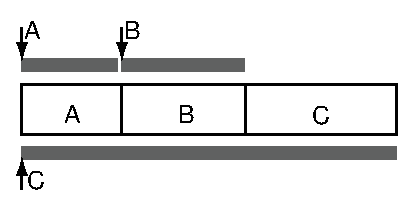
\includegraphics[scale=0.75]{c++-object}
\end{center}
%
The object $A$ is laid out first, followed by $B$, then any additional fields in $C$.  A pointer to
a $C$ object is also a pointer to an $A$, so this coercion has no runtime cost.  The coercion from
$C$ to $B$ is also allowed with a bit of pointer arithmetic.

In OCaml, the situation is quite different.  The order of methods and fields in an object doesn't
matter, coercions to arbitrary supertypes are allowed, and coercions never have a runtime cost.  To
help understand how this works, let's build a model of objects using polymorphic variants.

Abstractly, an object is just a thing that reacts to messages that are sent to it---in other words,
it is a function on method names.  Given an object $o$ with method names $m_1, m_2, \ldots, m_n$, the
names are given variant labels \hbox{\lstinline/`L_m1/}, \hbox{\lstinline/`L_m2/}, $\ldots$, \hbox{\lstinline/`L_mn/}.  The
object becomes a pattern match over method labels, and the fields become let-definitions.
Here is a dog object together with the corresponding model.

\begin{center}
\begin{tabular}{c|c}
Object & Model\\
\hline
\begin{minipage}[t]{2.2in}
\begin{ocamllisting}
type dog =
   < eat : unit;
     bark : unit;
     chase : string -> unit
   >

let dog s =
object (self)
   val name = s
   method eat = printf "%s eats\n" name
   method bark = printf "%s barks\n" name
   method chase s =
      self#bark;
      printf "%s chases %s\n" name s
end
\end{ocamllisting}
\end{minipage}
&
\begin{minipage}[t]{2.2in}
\begin{ocamllisting}
! type model_dog =
!    l:[`L_eat | `L_bark | `L_chase] -> 
!       (match l with
!           `L_eat | `L_bark -> unit
!         | `L_chase -> (string -> unit))

let model_dog s =
   let name = s in
   let rec self = function
      `L_eat -> printf "%s eats\n" name
    | `L_bark -> printf "%s barks\n" name
    | `L_chase -> (fun s ->
          self `L_bark;
          printf "%s chases %s\n" name s)
   in
   self
\end{ocamllisting}
\end{minipage}
\end{tabular}
\end{center}
%
The recursive function \hbox{\lstinline/self/} represents the object.  It takes a method label, and returns
the method value.  The type \hbox{\lstinline/model_dog/} can't be defined in OCaml, because it is
a \emph{dependent} type.  Informally it says that a \hbox{\lstinline/model_dog/} is a function that takes a
label \hbox{\lstinline/l/}.  If \hbox{\lstinline/l/} is \hbox{\lstinline/`L_eat/} or \hbox{\lstinline/`L_bark/}, then the result
type is \hbox{\lstinline/unit/}.  If the label is \hbox{\lstinline/`L_chase/}, the result type
is \hbox{\lstinline/string -> unit/}.

\begin{enumerate}
\item Suppose an animal object is defined as follows.

\begin{ocaml}
type animal = < eat : unit >
let animal s = object method eat = printf "%s eats\n" s end
\end{ocaml}
%
Write the model \hbox{\lstinline/model_animal/} for an animal object.

\item
Given a \hbox{\lstinline/model_dog/} $e$, how is a coercion \hbox{\lstinline/($e$ : model_dog :> model_animal)/} implemented?

\item
How is a coercion \hbox{\lstinline/($e$ : dog :> < chase : string -> unit >)/} implemented in the model?
\end{enumerate}
%
Suppose that, instead of representing fields as individual let-definitions, the fields of an object
are collected in a record, with the compiler inserting the appropriate projections.  For example,
here is a revised \hbox{\lstinline/model_dog/}.

\begin{ocaml}
type dog_fields = { name : string }

let model_dog s =
   let rec self fields = function
      `L_eat -> printf "%s eats\n" fields.name
    | `L_bark -> printf "%s barks\n" fields.name
    | `L_chase -> (fun s ->
          self fields `L_bark;
          printf "%s chases %s\n" fields.name s)
   in
   self { name = s }
\end{ocaml}
%
\begin{enumerate}
\item[4.] In this revised version, how is a functional update implemented?
Explain your answer by giving the model for a new method

\begin{ocaml}
method new_dog s = {< name = s >}.
\end{ocaml}

\item[5.]
What is the complexity of method dispatch?  Meaning, given an arbitrary method label, how long does
it take to perform the pattern match?
\end{enumerate}
%
Suppose the pattern match is hoisted out of the object into a separate function \hbox{\lstinline/vtable/}.

\begin{ocaml}
let model_dog s =
   let vtable = function
      `L_eat -> (fun self fields -> printf "%s eats\n" fields.name)
    | `L_bark -> (fun self fields -> printf "%s barks\n" fields.name)
    | `L_chase -> (fun self fields s ->
          self fields `L_bark;
          printf "%s chases %s\n" fields.name s)
   in
   let rec self fields label =
      vtable label self fields
   in
   self { name = s }
\end{ocaml}
%
\begin{enumerate}
\item[6.]  What are the advantages of the separate \hbox{\lstinline/vtable/}?  What are some disadvantages?
\end{enumerate}

\begin{answer}\ifanswers
\begin{enumerate}
\item 

\begin{ocaml}
let animal_model s =
   let rec self = function
      `L_eat -> printf "%s eats\n" s
   in
   self
\end{ocaml}

\item

A \hbox{\lstinline/model_dog/} has all the methods of a \hbox{\lstinline/model_animal/} so it can be used as an
animal unchanged.  The coercion returns the dog without change.  To be more precise, consider the
types.

\begin{ocaml}
type model_dog = l:[`L_eat | `L_bark | `L_chase] -> $\cdots$
type model_animal = l:[`L_eat] -> $\cdots$
\end{ocaml}
%
The relation \hbox{\lstinline/model_dog $\subtype$ model_animal/} holds because
\hbox{\lstinline/[`L_eat] $\subtype$ [`L_eat | `L_bark | `L_chase]/}.

\item 

A \hbox{\lstinline/model_dog/} can be used as a model-\hbox{\lstinline/< chase : string -> unit>/} without change.

\item

A functional update becomes a record update.
The new method \hbox{\lstinline/new_dog/} is modeled as follows.

\begin{ocaml}
let model_dog s =
   let rec self fields = function
      $\cdots$
    | `L_new_dog s ->
        self { fields with name = s }
   in
   self { name = s }
\end{ocaml}

\item

The pattern match is really just a table lookup, so it can be implemented in $O(\log n)$ time, where
$n$ is the number of labels.  However, the number of labels in the program is fixed, so the pattern
match can be implemented in constant time.

\item

The advantage of hoisting the \hbox{\lstinline/vtable/} is that it can be shared by multiple dog objects.
The disadvantage is that it may be slightly more expensive because of the extra function call.
\end{enumerate}
\fi\end{answer}      
\end{exercise}

% -*-
% Local Variables:
% Mode: LaTeX
% fill-column: 100
% TeX-master: "paper"
% TeX-command-default: "LaTeX/dvips Interactive"
% End:
% -*-
% vim:tw=100:fo=tcq:

\labelchapter{classes}{Classes and inheritance}

The simple objects that we have seen so far provide abstraction, but they provide
little in the way of software re-use, which is one of the key benefits of object-oriented
programming.  What exactly is object-oriented programming?  Mitchell~\cite{Mit03} points out four
fundamental properties.

\begin{itemize}
\item

\emph{Abstraction}:
the details of the implementation are hidden in the object; the interface is just the set of
publically-accessible methods.

\item

\emph{Subtyping}:
if an object \hbox{\lstinline/a/} has all the functionality of an object \hbox{\lstinline/b/}, then we may
use \hbox{\lstinline/a/} in any context where \hbox{\lstinline/b/} is expected.

\item

\emph{Dynamic lookup}:
when a message is sent to an object, the method to be executed is determined by the implementation
of the object, not by some static property of the program.  In other words, different objects may
react to the same message in different ways.

\item

\emph{Inheritance}:
the definition of one kind of object can be re-used to produce a new kind of object.
\end{itemize}
%
We have seen a little about first three features; we now look at inheritance.  In OCaml, like
many other languages, inheritance arises from classes, where a \emph{class} is a \emph{template}
that describes how to build an object.  Inheritance is the ability to create new classes (and thus
new objects) from existing ones by adding, removing, and modifying methods and fields.

\section{Class basics}

\index{classes!definitions}
\index{objects!classes}
Let's begin by defining a class.  The simplest form of a class definition looks like the definition
of an object, but using the keyword \hbox{\lstinline/class/} instead of \hbox{\lstinline/let/}.  Classes are not
objects in OCaml, and a class definition is not an expression.  Every class definition must occur at
the top level.

\label{keyword:class}
\begin{ocaml}
# class poly =
  object
     val vertices = [|(46, 70); (54, 70); (60, 150); (40, 150)|]
     method draw = Graphics.fill_poly vertices
  end;;
@
\begin{topoutput}
class poly : object val vertices : (int * int) array method draw : unit end
\end{topoutput}
@
\end{ocaml}
%
\index{new@\lstinline/new/}
\index{classes!new}
\label{keyword:new}
To create an object from a class, the keyword \hbox{\lstinline/new/} is used with the name of the class.

\begin{center}
\begin{tabular}{cc}
\begin{minipage}[b]{3in}
\begin{ocamllistingx}
# let p = new poly;;
@
\begin{topoutput}
val p : poly = <obj>
\end{topoutput}
@
# p#draw;;
@
\begin{topoutput}
- : unit = ()
\end{topoutput}
@
\end{ocamllistingx}
\end{minipage}
&
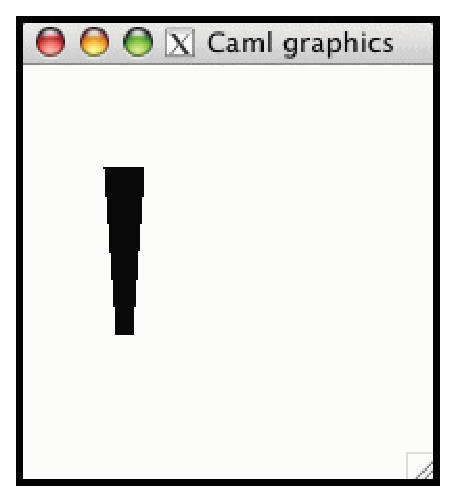
\includegraphics[scale=0.3]{graphics5}
\end{tabular}
\end{center}

\subsection{Class types}

There are a number of things happening here, so let's look at the parts.  First, we defined a
class called \hbox{\lstinline/poly/} with field \hbox{\lstinline/vertices/} and a method \hbox{\lstinline/draw/}.  The
class \hbox{\lstinline/poly/} has a \emph{class type} that specifies the type of its methods and fields.

\begin{ocaml}
object
   val vertices : (int * int) array
   method draw : unit
end
\end{ocaml}
%
\label{classes:types}
\index{class types}
Class types are something you may not have seen before, even if you are familiar with
object-oriented programming.  However, class types arise naturally in languages that include both
classes and modules.  In OCaml, every definition that can appear in a module must have a type.  A
class is not a type (because it contains code), so it must have a type.  Consider a module that
defines the blobs of the previous chapter.  The module \hbox{\lstinline/Blobs/} contains the class
definition, and the signature \hbox{\lstinline/BlobsSig/} declares the class and its type.

\begin{ocaml}
module Blobs : BlobsSig = struct         module type BlobsSig = sig
   class poly =                             class poly : 
   object                                   object
      val vertices = [||]                      val vertices : (int * int) array
      method draw =                            method draw : unit
         Graphics.fill_poly vertices        end
   end

   let p = new poly                         val p : poly
end;;                                    end;;
\end{ocaml}
%
Another thing to point out is that the polygon \hbox{\lstinline/p/} has type \hbox{\lstinline/val p : poly/}.
In this context, the class name \hbox{\lstinline/poly/} stands for the type of polygon
objects---that is, \hbox{\lstinline/type poly = < draw : unit >/}.  In general, whenever a class name appears in
the context of a type expression, it stands for an object type.  There is nothing special about the
class name.  Two classes that have methods with the same types stand for the same object type, as the
following example illustrates.

\index{gunfighter}
\begin{tabular}{l}
\begin{ocaml}
# class gunfighter =
  object
     method draw = print_string "Bang!\n"
  end;;
@
\begin{topoutput}
class gunfighter : object method draw : unit end
\end{topoutput}
@
# let p : gunfighter = new poly;;
@
\begin{topoutput}
val p : gunfighter = <obj>
\end{topoutput}
@
\end{ocaml}
\end{tabular}

\subsection{Parameterized classes}

\label{classes:parameterized}
\index{classes!constructors}
\index{classes!parameterized classes}
The current \hbox{\lstinline/poly/} class is not very useful because the vertices are fixed.  If we want
more than one polygon, we can define a \emph{parameterized class}.  A parameterized class definition
looks like a class definition that takes arguments; the arguments are passed to \hbox{\lstinline/new/} at
object creation time.

\begin{center}
\begin{tabular}{@{}cc}
\begin{minipage}[b]{3.5in}
\begin{ocamllistingx}
# class poly vertices =
  object
     val vertices = vertices
     method draw = Graphics.fill_poly vertices
  end;;
@
\begin{topoutput}
class poly : (int * int) array ->
  object val vertices : (int * int) array method draw : unit end
\end{topoutput}
@
# let p1 =
     new poly [|(46, 70); (54, 70); (60, 150); (40, 150)|];;
@
\begin{topoutput}
val p1 : poly = <obj>
\end{topoutput}
@
# let p2 = new poly [|(40, 40); (60, 40); (60, 60); (40, 60)|];;
@
\begin{topoutput}
val p2 : poly = <obj>
\end{topoutput}
@
# p1#draw; p2#draw;;
@
\begin{topoutput}
- : unit = ()
\end{topoutput}
@
\end{ocamllistingx}
\end{minipage}
&
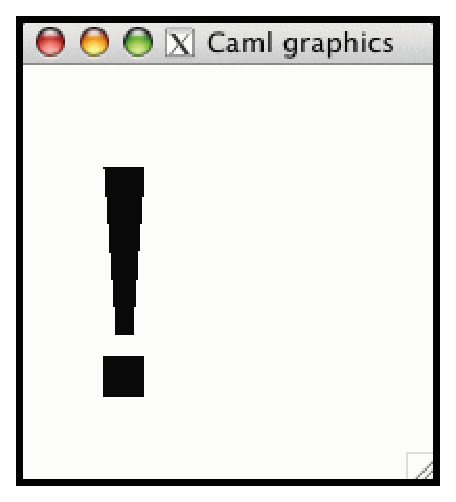
\includegraphics[scale=0.3]{graphics6}
\end{tabular}
\end{center}
%
In OCaml, there is no specific language feature called an object constructor.  Instead, the class
definition serves as its only constructor, and there is only one way to construct an object from a
class---by using \hbox{\lstinline/new/}.

In a class definition, any class expression can be used as the definition.  For example, the
following definition specifies that the class \hbox{\lstinline/rectangle/} is a specific kind
of \hbox{\lstinline/poly/}.

\begin{ocaml}
# class rectangle (x1, y1) (x2, x2) =
     poly [|(x1, y1); (x2, y1); (x2, y2); (x1, y2)|];;
@
\begin{topoutput}
class rectangle : float * float -> float * float -> poly
\end{topoutput}
@
\end{ocaml}

\subsection{Classes with let-expressions}

\label{classes:let}
\label{classes!let expressions}
Classes can be defined with leading let-definitions, which are evaluated before a new object is
created.  The let-definitions have the standard form.  For example, the following class defines a
regular polygon with \hbox{\lstinline/n/} sides.  The vertices of the polygon are computed before the
object is created.

\begin{ocaml}
class regular_poly n radius =
   let () = assert (n > 2) in
   let vertices = Array.create n (0, 0) in
   let step = 6.28 /. float_of_int n in
   let () =
      for i = 0 to n - 1 do
         let theta = float_of_int i *. step in
         let x = int_of_float (cos theta *. radius) in
         let y = int_of_float (sin theta *. radius) in
         vertices.(i) <- (x + 100, y + 100)
      done
   in
   object
      method draw = Graphics.fill_poly vertices
   end;;
\end{ocaml}
%
Syntactically, each leading expression must be a let-definition, so any computations that operate by
side-effect are written with a dummy let in the form \hbox{\lstinline/let () = $\cdots$ in/}.  The
assertion ensures that the polygon has at least 3 sides.

\begin{center}
\begin{tabular}{cc}
\begin{minipage}[b]{3in}
\begin{ocamllistingx}
# let p = new regular_poly 7 100.0;;
@
\begin{topoutput}
val p : regular_poly = <obj>
\end{topoutput}
@
# p#draw;;
@
\begin{topoutput}
- : unit = ()
\end{topoutput}
@
\end{ocamllistingx}
\end{minipage}
&
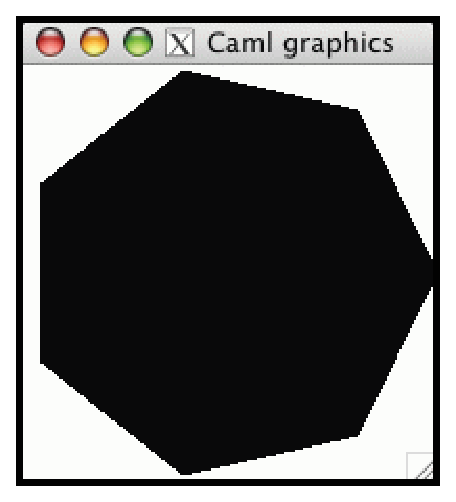
\includegraphics[scale=0.3]{regular-poly}
\end{tabular}
\end{center}

\subsection{Type inference}

\index{classes!type inference}
\index{classes!polymorphic}
If you have tried defining classes of your own, you may be running into a problem where OCaml is
inferring class types that are ``too polymorphic.''  Class types can be polymorphic, as we will see
in Chapter~\ref{chapter:polyclasses}, but the polymorphism must be written explicitly.  Consider the
following class definition, which is rejected by the compiler.

\begin{ocaml}
# class cell x =
  object
     method get = x
  end;;
@
\begin{topoutput}
...
Some type variables are unbound in this type:
  class cell : 'a -> object method get : 'a end
The method get has type 'a where 'a is unbound
\end{topoutput}
@
\end{ocaml}
%
The problem is that the argument \hbox{\lstinline/x/} has polymorphic type, so the class also has a
polymorphic type.  We won't bother much with polymorphic classes at this point, except to say that
if you really want one, then 1) you must write the type variables in square brackets before the
class name, and 2) you should read Chapter~\ref{chapter:polyclasses} before you do so.

\begin{ocaml}
# class ['a] cell (x : 'a) =
  object
     method get = x
  end;;
@
\begin{topoutput}
class ['a] cell : 'a -> object method get : 'a end
\end{topoutput}
@
\end{ocaml}
%
In many cases, polymorphic classes are inadvertant.  Suppose we copy the definition of the
polygon object from the previous chapter.

\begin{ocaml}
# class poly vertices =
object
   val vertices = vertices
   method draw = Graphics.fill_poly (Array.map int_coord vertices)
   method transform matrix = {< vertices = Array.map matrix#transform vertices >}
end;;
@
\begin{topoutput}
...
The method transform has type
  (< transform : float * float -> float * float; .. > as 'b) -> 'a
where 'b is unbound
\end{topoutput}
@
\end{ocaml}
%
This class definition is rejected because the method \hbox{\lstinline/transform/} takes
a \hbox{\lstinline/matrix/} that has an open, thus polymorphic, method type.  We really didn't mean to write
a polymorphic class, it is just that the type that was inferred is polymorphic.  There are two easy
solutions: constrain the type so that it is not polymorphic, or use a polymorphic method type.
Constraining the type so that it is not polymorphic is easy.

\begin{ocaml}
# type coord = float * float;;
@
\begin{topoutput}
type coord = float * float
\end{topoutput}
@
# class poly vertices =
object
   val vertices = vertices
   method draw = Graphics.fill_poly (Array.map int_coord vertices)
   method transform (matrix : < transform : coord -> coord >) =
      {< vertices = Array.map matrix#transform vertices >}
end;;
@
\begin{topoutput}
class poly : coord array -> ...
\end{topoutput}
@
\end{ocaml}
%
Using a polymorphic method type is almost as easy.  The method \hbox{\lstinline/transform/} has to be
written with the type right after the method name, using an open object type
\hbox{\lstinline/< transform : fcoord -> fcoord; .. > as 'a/} for the \hbox{\lstinline/matrix/} argument.

\begin{ocaml}
class poly vertices =
object (self : 'self)
   val vertices = vertices
   method draw = Graphics.fill_poly (Array.map int_coord vertices)
   method transform : 'a. (< transform : coord -> coord; .. > as 'a) -> 'self =
      (fun matrix -> {< vertices = Array.map matrix#transform vertices >})
end;;
\end{ocaml}
%
The leading \hbox{\lstinline/'a./} is a type quantifier.  It indicates that the type variable belongs
specifically to the method \hbox{\lstinline/transform/}, not to the class as a whole.  We'll see more about
polymorphic methods in Section~\ref{section:poly-methods}.

\section{Inheritance}

\index{inheritance}
\index{classes!inheritance}
\index{classes!sub- and super-classes}
\index{classes!is-a}
Generally speaking, inheritance is the ability to define
new classes by re-using existing ones.  In the normal case, a new class is created by adding methods
and fields to an existing class, or by changing its method implementations, or both.  When a class
$B$ inherits from a class $A$, we say that $B$ is a \emph{subclass} of $A$, and $A$ is
a \emph{superclass} of $B$.  When $B$ also defines a subtype of $A$ (so that an object of class $B$
can be used anywhere than an object of class $A$ is expected), we say that the relationship is an
``is-a'' relationship.  Is-a relationships are the most common form of inheritance, and in standard
programming practice most, if not all, inheritance relationships are is-a relationships.

This notion leads to a programming model where an inheritance hierarchy is conceived in terms of the
is-a relationship.  Some examples are shown in Figure~\ref{figure:inheritance-examples}, where the
arrows point from subclass to immediate superclass.  For example the class \hbox{\lstinline/square/}
inherits from the class \hbox{\lstinline/rectangle/} (and a square is-a rectangle).

\begin{figure}
\centerline{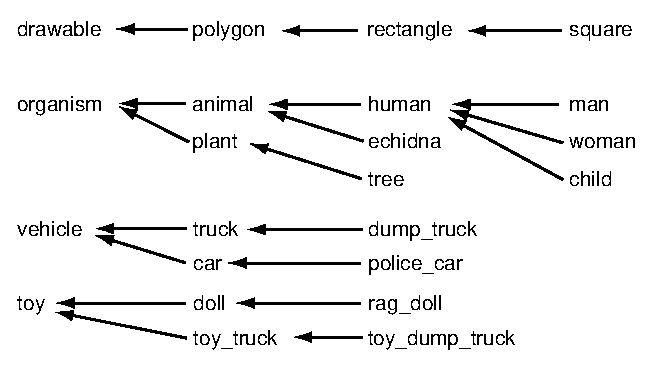
\includegraphics[scale=0.75]{hierarchy}}
\caption{Example inheritance hierarchies.}
\label{figure:inheritance-examples}
\end{figure}

\label{keyword:inherit}
\index{inherit@\lstinline/inherit/}
Concretely, a class inherits from another with the directive
\hbox{\lstinline/inherit $\nt{class-expression}$/},
which effectively includes the entire class $\nt{class-expression}$ within the current one. To
illustrate, let's build a simple model of a part of the animal kingdom.  The following diagram
lists the class hierarchy and methods: every animal eats; a pet is an animal with an owner and a
name; and a pet dog is a pet that barks.

\begin{center}
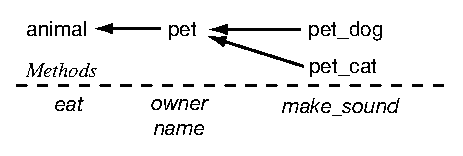
\includegraphics[scale=0.75]{animal1}
\end{center}
%
At the root of the hierarchy is the class \hbox{\lstinline/animal/}, which has a single method \hbox{\lstinline/eat/}.

\begin{ocaml}
# class animal species =
  object
     method eat = Printf.printf "A %s eats.\n" species
  end;;
@
\begin{topoutput}
class animal : string -> object method eat : unit end
\end{topoutput}
@
\end{ocaml}
%
A pet is an animal with an owner and a name.  The class \hbox{\lstinline/pet/} defines
methods \hbox{\lstinline/owner/} and \hbox{\lstinline/name/}, and it also \emph{inherits} from the
class \hbox{\lstinline/animal/}.  The effect of the inheritance is like inclusion, as if the methods of
class \hbox{\lstinline/animal/} were included in the class \hbox{\lstinline/pet/}.

\begin{ocaml}
# class pet ~species ~owner ~name =
  object
     inherit animal species
     method owner : string = owner
     method name  : string = name
  end;;
@
\begin{topoutput}
class pet : species:string -> owner:string -> name:string ->
  object method name : string method owner : string method eat : unit end
\end{topoutput}
@
\end{ocaml}
%
The class \hbox{\lstinline/pet_dog/} is a particular kind of pet that barks.  Once again, the result of the
inheritance is exactly like inclusion.  The class \hbox{\lstinline/pet_dog/} includes the methods of
class \hbox{\lstinline/pet/}, which in turn includes the methods of the class \hbox{\lstinline/animal/}.  The
result is a class that includes all the methods of all the ancestor classes.

\begin{ocaml}
# class pet_dog ~owner ~name =
  object
     inherit pet ~species:"dog" ~owner ~name
     method speak = Printf.printf "%s barks!\n" name
  end;;
@
\begin{topoutput}
class pet_dog : owner:string -> name:string ->
  object
    method speak : unit
    method name : string
    method owner : string
    method eat : unit
  end
\end{topoutput}
@
# let clifford = new pet_dog ~name:"Clifford" ~owner:"Emily";;
@
\begin{topoutput}
val clifford : pet_dog = <obj>
\end{topoutput}
@
# clifford#speak;;
@
\begin{topoutput}
Clifford barks!
\end{topoutput}
@
# clifford#eat;;
@
\begin{topoutput}
A dog eats.
\end{topoutput}
@
\end{ocaml}

\subsection{Method override}

\index{classes!method override}
These previous two examples of inheritance are both forms of specialization where the inheriting
class includes the behavior of the superclass but does not modify it.  It is also possible for a
subclass to modify the behavior by redefining its methods.  For example, since a pet has a name, we
may wish to use the pet's name instead of the species name when it eats.  We can do this by
redefining the method \hbox{\lstinline/eat/}.

\begin{ocaml}
# class pet ~species ~owner ~name =
object
   inherit animal species
   method owner : string = owner
   method name : string = name
   method eat = Printf.printf "%s eats.\n" name
end;;
@
\begin{topoutput}
class pet : species:string -> owner:string -> name:string ->
  object method name : string method owner : string method eat : unit end
\end{topoutput}
@
\end{ocaml}
%
Some dogs are protective about their food.  We can capture this by further
redefining the method \hbox{\lstinline/eat/}.

\begin{ocaml}
# class pet_dog ~owner ~name =
  object (self : 'self)
     inherit pet ~species:"Dog" ~owner ~name as super
     method speak = Printf.printf "%s barks!\n" name
     method prepare_to_eat =
        Printf.printf "%s growls menacingly.\n" name
     method eat =
        self#prepare_to_eat;
        super#eat
  end;;
@
\begin{topoutput}
class pet_dog : ...
\end{topoutput}
@
# let clifford = new pet_dog ~owner:"Emily" ~name:"Clifford";;
@
\begin{topoutput}
val clifford : pet_dog = <obj>
\end{topoutput}
@
# clifford#eat;;
@
\begin{topoutput}
Clifford growls menacingly.
Clifford eats.
\end{topoutput}
@
\end{ocaml}
%
\index{classes!naming a superclass}
The syntax \hbox{\lstinline/inherit $\nt{class-expression}$ as $\nt{identifier}$/} gives a name to the
superclass, which allows the superclass methods to be invoked.  This is useful mainly when the
superclass's methods are overridden in the subclass.  In this case, the method \hbox{\lstinline/eat/} in the
class \hbox{\lstinline/pet_dog/} is a kind of ``wrapper'' method.  It overrides
the \hbox{\lstinline/pet/}'s \hbox{\lstinline/eat/} method by first preparing to eat, then calling the
pet-eat method with the expression \hbox{\lstinline/super#eat/}.

\subsection{Class types}

The design of the inheritance hierarchy can have a major impact on the ease of programming a
system.  This is particularly true for languages based on nominal typing, like C++ or Java, where
subtyping is constrained by the hierarchy.  For example, in a nominal type scheme,
the type of an object corresponds to the class name, so a \hbox{\lstinline/pet_dog/} can be coerced to
a \hbox{\lstinline/pet/}, and then to an \hbox{\lstinline/animal/}, but no other coercions are allowed.

This can be overly restrictive of course.  As the design proceeds we might discover we need new classes.
For the animal example, we might want a class \hbox{\lstinline/farm_animal/}, where animals have owners but
might not have names; or a class \hbox{\lstinline/vocal_animal/} for animals that can vocalize, but might
be wild.  A \hbox{\lstinline/dog/} can be a \hbox{\lstinline/pet/}, a \hbox{\lstinline/farm_animal/}, and also
a \hbox{\lstinline/vocal_animal/}.

In the worst case, the inheritance hierarchy can become complicated because the number of feature
sets is combinatorial.  Languages with interfaces, like Java, try to combat this problem by allowing
a class to satisfy multiple interface definitions.

\begin{java}
interface farm_animal { void eat(); String owner(); };
interface vocal_animal { void eat(); void speak(); }
class dog extends pet implements farm_animal, vocal_animal { $\cdots$ }
\end{java}
%
One drawback of this approach is that the interfaces must be specified at class definition time,
requiring the designer to predict what the useful interfaces will be.

In OCaml, the situation is different.  The inheritance hierarchy constrains the way in which classes
are specified and implemented, but it has no effect on subtyping.  Here is how we could extend the
animal example to support farm animals and vocal animals.

\label{classes:type-inherit}
\begin{ocaml}
# class type farm_animal =
  object
     inherit animal
     method owner : string
  end;;
@
\begin{topoutput}
class type farm_animal = object method owner : string method eat : unit end
\end{topoutput}
@
# class type vocal_animal =
  object
     inherit animal
     method speak : unit
  end;;
@
\begin{topoutput}
class type vocal_animal = object method speak : unit method eat : unit end
\end{topoutput}
@
# (clifford : pet_dog :> farm_animal);;
@
\begin{topoutput}
- : farm_animal = <obj>
\end{topoutput}
@
\end{ocaml}
%
Note that in the \hbox{\lstinline/inherit/} clause, the class type does not take arguments.  In this
context, the name \hbox{\lstinline/animal/} stands for the class type, and the \hbox{\lstinline/inherit/}
directive again acts as textual inclusion.

The main advantage of structural subtyping is that an object can be coerced to any compatible type,
the types do not have to be specified ahead of time.  The disadvantage of course, is that subtyping
may be overly permissive; some coercions might not make sense semantically.

\begin{ocaml}
# class cat ~owner ~name =
  object
     inherit pet ~species:"cat" ~owner ~name
     method speak = Printf.printf "%s meows.\n" name
  end;;
@
\begin{topoutput}
class cat : owner:string -> name:string ->
  object
    method speak : unit
    method name : string
    method owner : string
    method eat : unit
  end
\end{topoutput}
@
# let my_cat = (clifford :> cat);;
@
\begin{topoutput}
val my_cat : cat = <obj>
\end{topoutput}
@
# my_cat#speak;;
@
\begin{topoutput}
Clifford barks!
\end{topoutput}
@
\end{ocaml}

\subsection{Class type constraints and hiding}

\index{classes!type constraints}
\index{classes!hiding}
The type of a class can be constrained with the following syntax, where $\nt{class-type}$ is a class type.

\begin{ocaml}
class $\nt{class-name}$ $\nt{parameter}_1$ $\cdots$ $\nt{parameter}_n$ : $\nt{class-type}$ = $\nt{class-expression}$
\end{ocaml}
%
It is also possible to place constraints on the object type, with an explicit constraint of the form
\hbox{\lstinline/constraint 'self = $\nt{object-type}$/},
or equivalently using the syntax \hbox{\lstinline/$\nt{object-type}$ as 'self/}.

\begin{ocaml}
class cat ~name ~owner =
object (self : 'self)
   constraint 'self = < eat : unit; speak : unit; .. >
   inherit pet ~name ~owner
   method speak = Printf.printf "%s meows.\n" name
end
\end{ocaml}
%
As a programmer, you might want to write a type constraint to ensure that your implementation
matches a specified interface.  However, there are other reasons for using a type constraint.
Unlike the rest of OCaml, type constraints on classes can change how the program behaves.
Here is what you can (and cannot) do with a constraint.

\begin{enumerate}
\item A constraint \emph{cannot} be used hide public methods.
\item A constraint can be used to turn a private method into a public method.
\item A constraint can be used to hide fields and private methods.
\end{enumerate}
%
The restriction on public methods is the same as it is for object types.
If an object has a public method, the method must appear in the type.

\begin{ocaml}
# (object method x = 1 method y = 2 end : < x : int >);;
@
\begin{topoutput}
...
This expression has type < x : int; y : int > but is here used with type
  < x : int >
The second object type has no method y
\end{topoutput}
@
\end{ocaml}
%
The second property, where private methods are made public, may be a little surprising.  It is often
used in cases where a superclass defines a private method that a subclass would like to be made
public.

\begin{ocaml}
# class foo =
  object (self : 'self)
     constraint 'self = < x : int; .. >
     method private x = 1
  end;;
@
\begin{topoutput}
class foo : object method x : int end
\end{topoutput}
@
\end{ocaml}
%
The third kind of constraint, used to hide field and private methods, requires some discussion.
When a class hides a field, or a private method, that field becomes inaccessible to subclasses, and
it also means that the field or method cannot be overridden.  Consider the following class
definitions.

\begin{ocaml}
# class a =
object (self)
   method private f_private = print_string "aaaa\n"
   method test_a = self#f_private
end;;
# class b =
object (self)
   inherit a
   method private f_private = print_string "bbbb\n"
   method test_b =
      self#test_a;
      self#f_private
end;;
# (new b)#test_b;;
@
\begin{topoutput}
bbbb
bbbb
\end{topoutput}
@
\end{ocaml}
%
The method \hbox{\lstinline/f_private/} is private, but it is the same method in both classes.  The definition
of \hbox{\lstinline/f_private/} in class \hbox{\lstinline/b/} \emph{overrides} the definition in class \hbox{\lstinline/a/},
so the result is to print \hbox{\lstinline/bbbb/} twice.
Now let's consider what happens when \hbox{\lstinline/f_private/} is hidden by a type constraint.

\begin{ocaml}
# class type a_type = object method test_a : unit end;;
# class a : a_type =
  object (self)
     method private f_private = print_string "aaaa\n"
     method test_a = self#f_private
  end;;
# class b = $\cdots\hbox{\textit{same as before}}\cdots$;;
# (new b)#test_b;;
@
\begin{topoutput}
aaaa
bbbb
\end{topoutput}
@
\end{ocaml}
%
In this case, the result is different.  By hiding the method \hbox{\lstinline/f_private/} in
class \hbox{\lstinline/a/}, it can't be used or overridden in subclass \hbox{\lstinline/b/}, and the behavior of
the program is changed.

The property is the same for fields.  When a field is hidden y a type constraint, it is no longer
accessible to subclasses.  New field definitions with the same name in subclasses are independent.
  
\subsection{Classes and class types as object types}

As we have mentioned, a class is not a type, but the class name stands for an object type
when used in the context of a type expression.  The same holds for class types---a class type is the
type of a class, but it also stands for the type of an object when used in context of a type
expression.  The object type is formed from a class type by omitting the field types.
The following table lists some examples of equivalent types.

\begin{center}
\begin{tabular}{lll}
Class type & Object type & Simplified\\
\hline
\begin{minipage}[t]{1.5in}
\begin{ocamllisting}
class type t1 =
object
   val x : int
   method y : int
end
\end{ocamllisting}
\end{minipage}
&
\begin{minipage}[t]{1.5in}
\begin{ocamllisting}
type t1 = < y : int >
\end{ocamllisting}
\end{minipage}
\\
\begin{minipage}[t]{1.5in}
\begin{ocamllisting}
class type t2a =
object ('self)
   val x : int
   method f1 : t2a
   method f2 : 'self  
end

class type t2b =
object ('self)
   inherit t2a
   method f3 : unit
end
\end{ocamllisting}
\end{minipage}
&
\begin{minipage}[t]{1.5in}
\begin{ocamllisting}
type t2a =
   < f1 : t2a;
     f2 : 'self
    > as 'self



type t2b =
   < f1 : t2a;
     f2 : 'self;
     f3 : unit
   > as 'self
\end{ocamllisting}
\end{minipage}
&
\begin{minipage}[t]{1in}
\begin{ocamllisting}
type t2a =
   < f1 : t2a;
     f2 : t2a
    >



type t2b =
   < f1 : t2a;
     f2 : t2b;
     f3 : unit
   >
\end{ocamllisting}
\end{minipage}
\end{tabular}
\end{center}
%
The role of \hbox{\lstinline/'self/} in these types is subtle and important.  In class
type \hbox{\lstinline/t2a/}, the method \hbox{\lstinline/f1/} returns an object of type \hbox{\lstinline/t2a/}, which
means that it is an object with exactly two methods, \hbox{\lstinline/f1/} and \hbox{\lstinline/f2/}.  The
method \hbox{\lstinline/f2/} returns an object of the same type as \hbox{\lstinline/self/}---which,
for an object of type \hbox{\lstinline/t2a/}, has the same methods \hbox{\lstinline/f1/} and \hbox{\lstinline/f2/}.

However, when the subclass \hbox{\lstinline/t2b/} is formed, a new method \hbox{\lstinline/f3/} is added.  The
method \hbox{\lstinline/f1/} returns an object of type \hbox{\lstinline/t2a/}, having two methods \hbox{\lstinline/f1/}
and \hbox{\lstinline/f2/}; but the method \hbox{\lstinline/f2/} returns an object of type \hbox{\lstinline/'self/},
now having three methods \hbox{\lstinline/f1/}, \hbox{\lstinline/f2/}, and \hbox{\lstinline/f3/}.

\label{keyword:hash-class}
\index{classes!\#types@\lstinline/#/types}
\index{\#!class types}
There are actually two kinds of object types that are formed from class names: exact and open types.
The type expression $\nt{class-name}$ stands for the type of objects having exactly the
methods of the class $\nt{class-name}$ and the type expression \hbox{\lstinline/#$\nt{class-name}$/}
stands for objects having those methods, and possibly more.  In other words, a type expression
\hbox{\lstinline/#$\nt{class-name}$/} stands for an open object type.

\begin{center}
\begin{tabular}{ll}
Type expression & Object type\\
\hline
\begin{minipage}[t]{2in}
\begin{ocamllisting}
t1
#t1
\end{ocamllisting}
\end{minipage}
&
\begin{minipage}[t]{2in}
\begin{ocamllisting}
< y : int >
< y : int; .. >
\end{ocamllisting}
\end{minipage}
\\
\begin{minipage}[t]{2in}
\begin{ocamllisting}
t2a
#t2a
\end{ocamllisting}
\end{minipage}
&
\begin{minipage}[t]{2in}
\begin{ocamllisting}
< f1 : t2a; f2 : 'self > as 'self
< f1 : t2a; f2 : 'self; .. > as 'self
\end{ocamllisting}
\end{minipage}
\\
\begin{minipage}[t]{2in}
\begin{ocamllisting}
#t2b
\end{ocamllisting}
\end{minipage}
&
\begin{minipage}[t]{2in}
\begin{ocamllisting}
< f1 : t2a;
  f2 : 'self;
  f3 : unit;
  .. > as 'self
\end{ocamllisting}
\end{minipage}
\end{tabular}
\end{center}
%
Just like an open object type, a type expression \hbox{\lstinline/#$\nt{class-name}$/} is polymorphic.

\begin{ocaml}
# type s2a = #t2a;;
@
\begin{toperror}
Characters 4-15:
  type s2a = #t2a;;
      ^^^^^^^^^^^
A type variable is unbound in this type declaration.
In definition #t2a as 'a the variable 'a is unbound
\end{toperror}
@
# type 'a s2a = #t2a as 'a;;
@
\begin{topoutput}
type 'a s2a = 'a constraint 'a = #t2a
\end{topoutput}
@
\end{ocaml}

\section{Inheritance is not subtyping}

\index{classes!inheritance \emph{vs}. subtyping}
Let's summarize the operations that can be performed through inheritance.
One may:
%
\begin{itemize}
\item add new fields and new private methods,
\item add new public methods,
\item override fields or methods, but the type can't be changed.
\end{itemize}
%
Fields and private methods don't appear in the object type, and method override isn't allowed to
change the method's type.  So from a typing perspective, if a class $B$ is a subclass of $A$, it
might have more methods than $A$, but everything else is unchanged.  By width subtyping
(Section~\ref{section:width-subtyping}), this will usually mean that the object type for $B$ is a
subtype of the object type for $A$.  In fact, in many languages, subclassing and subtyping are the
same, and it isn't possible to have one without the other.

Unfortunately, the correspondence is sound only in the case where the object type is covariant
in \hbox{\lstinline/'self/}; in other words, when the object has no binary methods.  Consider a class
type \hbox{\lstinline/comparable/} for objects that can be compared.
\label{page:comparable}

\begin{ocaml}
(* less-than: negative; equal: zero; greater-than: positive *)
type comparison = int

class type comparable =
object ('self)
   method compare : 'self -> comparison
end
\end{ocaml}
%
The method \hbox{\lstinline/compare/} is a binary method; it takes another object of type \hbox{\lstinline/'self/}
and performs a comparison.  The implementations use the usual technique of adding a
method \hbox{\lstinline/representation/} to expose the internal representation so that the comparison can
be implemented.\footnote{Note that subtraction can only be used to compare small
integers.}

\begin{ocaml}
class int_comparable (i : int) =     class string_comparable (s : string) =
object                               object
   method representation = i            method representation = s
   method compare (j : 'self) =         method compare (s2 : 'self) =
      i - j#representation                 String.compare s s2#representation
end                                  end
\end{ocaml}
%
We might later decide to implement some subclasses for printable, comparable objects.
%
\begin{ocaml}
class int_print_comparable i =       class string_print_comparable s =
object (_ : 'self)                   object (_ : 'self)
   inherit int_comparable i             inherit string_comparable s
   method print = print_int i           method print = print_string s
end                                  end
\end{ocaml}
%
We might expect that a printable and comparable integer is also a comparable integer.  However, the
expected coercions fail.

\begin{ocaml}
# (new int_comparable 1 :> comparable);;
@
\begin{topoutput}
... This expression cannot be coerced ...
\end{topoutput}
@
# (new int_print_comparable 1 :> int_comparable);;
@
\begin{topoutput}
... This expression cannot be coerced ...
\end{topoutput}
@
\end{ocaml}
%
For an intuitive explanation, consider what would happen if the subtype relation
\hbox{\lstinline/int_comparable $\subtype$ comparable/} held.
The relation \hbox{\lstinline/string_comparable $\subtype$ comparable/} would hold as well, allowing us to
perform an unsound comparison of strings and integers.

\begin{ocaml}
(* !!FAKE--THESE OPERATIONS ARE UNSOUND!! *)
# let i = (new int_comparable 1 :> comparable);;
@
\begin{topoutput}
i : comparable = < obj >
\end{topoutput}
@
# let s = (new string_comparable "Hello" :> comparable);;
@
\begin{topoutput}
s : comparable = < obj >
\end{topoutput}
@
# i#compare s;;
@
\begin{topoutput}
???
\end{topoutput}
@
\end{ocaml}
%
The real problem is the the method \hbox{\lstinline/compare/} is \emph{contravariant} in the
type \hbox{\lstinline/'self/} because it takes a value of type \hbox{\lstinline/'self/} as an argument.  This is
the opposite of what it normally is.  Here are the object types that correspond to the classes and
class types.

\begin{ocaml}
comparable = < compare : 'self -> bool > as 'self
int_comparable =
   < representation : int;
     compare : 'self -> bool > as 'self
int_print_comparable =
   < representation : int;
     compare : 'self -> bool;
     print : unit > as 'self
\end{ocaml}
%
Let's try to carry out a proof of the subtyping relation
\hbox{\lstinline/int_comparable $\subtype$ comparable/}
to see where it goes wrong.  The type \hbox{\lstinline/'self/} in each case corresponds
to the type name, so we are try to show the following.

\begin{ocaml}
< representation : int; compare : int_comparable -> bool >
$\subtype$ < compare : comparable -> bool >
\end{ocaml}
%
Attempted proof:
\begin{itemize}
\item 
The types are recursive, so we first assume that subtyping holds on the type
names \hbox{\lstinline/int_comparable $\subtype$ comparable/}.
\item
By width subtyping, the method \hbox{\lstinline/representation/} can be dropped.
Show:
\begin{ocaml}
< compare : int_comparable -> bool > $\subtype$ < compare : comparable -> bool >
\end{ocaml}
\item
By depth subtyping, show:
\begin{ocaml}
(int_comparable -> bool) $\subtype$ (comparable -> bool)
\end{ocaml}
\item
By function subtyping, show:
\begin{ocaml}
comparable $\subtype$ int_comparable
\end{ocaml}
\item This is the opposite of the assumption, so the proof fails.
\end{itemize}

% \subsubsection{Generic functions and binary methods}

Of course, this doesn't mean that we can't write generic functions of comparable objects, it simply
means that the functions should use the open type \hbox{\lstinline/#comparable/}, not the exact
non-polymorphic type \hbox{\lstinline/comparable/}.

\begin{ocaml}
# let sort (l : #comparable list) = List.sort (fun e1 e2 -> e1#compare e2) l;;
@
\begin{topoutput}
val sort : (#comparable as 'a) list -> 'a list = <fun>
\end{topoutput}
@
# let l = List.map (new int_print_comparable) [9; 1; 6; 4];;
@
\begin{topoutput}
val l : int_print_comparable list = [<obj>; <obj>; <obj>; <obj>]
\end{topoutput}
@
# List.iter (fun i -> i#print) (sort l);;
@
\begin{topoutput}
1469
\end{topoutput}
@
\end{ocaml}

% \subsubsection{Bounded methods}

We might be willing to accept the fact that there are no useful objects with exact
type \hbox{\lstinline/comparable/}, but what about the relation between the
types \hbox{\lstinline/int_print_comparable/} and \hbox{\lstinline/int_comparable/}?  If it seems that the
subtyping relation should hold, the solution is to avoid the use of binary methods.  The
method \hbox{\lstinline/compare/} doesn't really need an argument of type \hbox{\lstinline/'self/},
it just needs an object with the same representation.  The classes can be reimplemented
to use a constrained argument type.

\begin{ocaml}
class int_comparable (i : int) =
object
   method representation = i
   method compare : 'a. (< representation : int; .. > as 'a) -> comparison =
      (fun j -> Pervasives.compare i j#representation)
end

class int_print_comparable i =
object
   inherit int_comparable i
   method print = print_int i
end
\end{ocaml}
%
It now holds that \hbox{\lstinline/int_print_comparable/} is a subtype of \hbox{\lstinline/int_comparable/}, but
there are several drawbacks.  One is that the new objects no longer have
type \hbox{\lstinline/#comparable/}, so it isn't possible to write truly generic functions.  Another
problem is that the types get quickly complicated.  Still, with some effort, we get what we want.

\begin{ocaml}
# let compare_int (e1 : #int_comparable) (e2 : #int_comparable) =
     e1#compare e2;;
@
\begin{topoutput}
val compare_int : #int_comparable -> #int_comparable -> comparison = <fun>
\end{topoutput}
@
# let sort_int (l : #int_comparable list) =
     List.sort compare_int l;;
@
\begin{topoutput}
val sort_int : (#int_comparable as 'a) list -> 'a list = <fun>
\end{topoutput}
@
# let l = List.map (new int_print_comparable) [9; 1; 3; 2];;
@
\begin{topoutput}
val l : int_print_comparable list = [<obj>; <obj>; <obj>; <obj>]
\end{topoutput}
@
# List.iter (fun i -> i#print) (sort_int l);;
@
\begin{topoutput}
1239
\end{topoutput}
@
\end{ocaml}

\labelsection{modules-classes}{Modules and classes}

OCaml includes two major systems for modularity and abstraction: the module system and the object
system.  In many respects, the two systems are quite similar.  Both provide mechanisms for
abstraction and encapsulation, for subtyping (by omitting methods in objects, and omitting fields in
modules), and for inheritance (objects use \hbox{\lstinline/inherit/}; modules use \hbox{\lstinline/include/},
Section~\ref{section:include}).  However, the two systems are not comparable.  On the one hand,
objects have an advantage: objects are first-class values, and modules are not---in other words,
modules do not support dynamic lookup.  On the other hand, modules have an advantage: modules
can contain type definitions, and objects cannot.

We have already suggested that modules are handy for hiding internal representations in the definition of
binary methods.  For example, let's use the module to hide the representation of a comparable object.

\begin{ocaml}
module type IntComparableSig =
sig
   type rep

   class int_comparable : int ->
   object ('self)
      method representation : rep
      method compare : 'self -> comparison
   end
end

module IntComparable : IntComparableSig =
struct
   type rep = int

   class int_comparable (i : int) =
   object (_ : 'self)
      method representation = i
      method compare (j : 'self) =
         Pervasives.compare i j#representation
   end
end
\end{ocaml}
%
This method of hiding the representation also has the side-effect that it is no longer possible to
construct an object of type \hbox{\lstinline/int_comparable/} without using the
class \hbox{\lstinline/int_comparable/}.  We can use this to our advantage.  In the animal example, if we
wish to ensure that dogs cannot be turned into cats, we can give the cats a ``certificate'' that
``justifies'' their authenticity.

\begin{ocaml}
module type CatSig =
sig
   type cert

   class cat : owner:string -> name:string ->
   object
      inherit pet
      method cert : cert
      method speak : unit
   end
end

module Cat : CatSig =
struct
   type cert = unit

   class cat ~owner ~name =
   object
       inherit pet ~species:"cat" ~owner ~name
       method cert = ()
       method speak = Printf.printf "%s meows.\n" name
   end
end
\end{ocaml}
%
\index{cat certificates}
It doesn't matter what the certificate is, just that it is abstract.  Of course, this technique
mainly prevents accidental coercions.  If a dog really wants to become a cat, it can take the
certificate from one of them.

Functors can also be useful in class construction.  For example, there are many specific kinds of
comparable objects, integers, floating-point values, strings, pairs of \hbox{\lstinline/comparable/}
objects, \emph{etc}.  All we need to build one of these is a function to compare the values.
The generic class is described the usual way.

\begin{ocaml}
(* less-than: negative; equal: zero; greater-than: positive *)
type comparison = int

class type comparable =
object ('self)
   method compare : 'self -> comparison
end;;
\end{ocaml}
%
To build a specific kind of comparable items, we need a function to compare the values.  We can build
a generic module as a functor that takes the type of items and the comparison as an argument, and produces
a new class of comparable items.

\begin{ocaml}
module type CompareSig =
sig
   type t
   val compare : t -> t -> comparison
end;;

module type ComparableSig =
sig
   type t
   type rep

   class element : t ->
   object ('self)
       method representation : rep
       method compare : 'self -> comparison
   end
end;;

module MakeComparable (Compare : CompareSig)
: ComparableSig with type t = Compare.t =
struct
   type t = Compare.t
   type rep = Compare.t

   class element (x : t) =
   object (self : 'self)
      method representation = x
      method compare (item : 'self) =
         Compare.compare x item#representation
   end
end;;
\end{ocaml}
%
The representation type \hbox{\lstinline/rep/} is abstract, but the type of element values \hbox{\lstinline/t/} is
not.  The method \hbox{\lstinline/compare/} simply uses the provided function \hbox{\lstinline/Compare.compare/}
to compare the representations.

\labelsection{poly-methods}{Polymorphic methods and virtual classes}

Let's turn to another example of object-oriented programming, this time more computational.
A \emph{collection}, in general, is like a set of elements.  There are many kinds of collections,
some based on implementations like arrays or lists, and others based on access patterns, like stacks
and queues.  Figure~\ref{figure:collection-hierarchy} shows a partial inheritance hierarchy.

\begin{figure}
\centerline{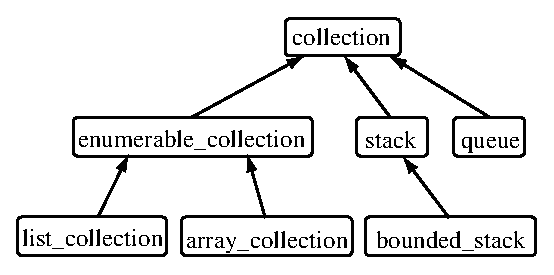
\includegraphics[scale=0.75]{collection}}
\caption{Hierarchy of collections}
\label{figure:collection-hierarchy}
\end{figure}

It won't matter much what the elements are, so for now we'll just assume the elements can be
printed.  It might also be useful to build polymorphic collections, but we'll leave that topic for
the Chapter~\ref{chapter:polyclasses}.

\begin{ocaml}
class type element = object method print : unit end
\end{ocaml}
%
At the root of the inheritance hierarchy is the type \hbox{\lstinline/collection/}, which represents the
features that all collections have in common.  What are those features?  It can't be implementation
or access pattern, because those features change for different kinds of collections.  In fact, the
type \hbox{\lstinline/collection/} by itself is pretty useless.  We'll assume it has a
method \hbox{\lstinline/length/} that returns the number of elements in the collection.

\begin{ocaml}
class type collection =
object
   method length : int
end
\end{ocaml}
%
At the middle of the hierarchy is the ``\hbox{\lstinline/enumerable_collection/},'' which represents
collections where the elements can be enumerated, using functions like \hbox{\lstinline/iter/} to iterate
over all the elements, or \hbox{\lstinline/fold/} to compute a value from all the elements.  The method types
correspond to the function types in the standard libraries \hbox{\lstinline/List/}
and \hbox{\lstinline/Array/}.  We still haven't implemented a concrete collection, so this is still a class
type.

\begin{ocaml}
class type enumerable_collection =
object
   inherit collection
   method iter : (element -> unit) -> unit
   method fold : ('a -> element -> 'a) -> 'a -> 'a
end;;
\end{ocaml}

\subsection{Polymorphic methods}

\index{classes!polymorphic methods}
Next, \hbox{\lstinline/list/} and \hbox{\lstinline/array/} are two concrete
kinds of collections that differ mainly in how they are accessed; a \hbox{\lstinline/list/} is a stack,
while an \hbox{\lstinline/array/} allows random access.  However, when we try to provide a concrete list
implementation, we encounter an error because the method \hbox{\lstinline/fold/} is polymorphic.

\begin{ocaml}
# class broken_list_collection =
  object
     $\cdots$
     method fold f x = List.fold_left f x elements
  end;;
@
\begin{toperror}
Characters 5-328: ...
Some type variables are unbound in this type:
...
The method fold has type ('a -> element -> 'a) -> 'a -> 'a where 'a
is unbound
\end{toperror}
@
\end{ocaml}
%
\label{types:polymorphic-methods}
The problem here is that OCaml assumes that
the \emph{class} must be polymorphic, not the \emph{method} (which is what we intend).  OCaml allows
methods to be polymorphic, but they must be annotated explicitly using the following syntax.

\begin{ocaml}
method $\nt{identifier}$ : '$\nt{type-variable}$ $\cdots$ '$\nt{type-variable}$. $\nt{type}$ = $\nt{expression}$
\end{ocaml}
%
\label{classes:type-quantifier}
The type expression \hbox{\lstinline/'$\nt{type-variable}$ $\cdots$ '$\nt{type-variable}$. $\nt{type}$/} is
called a \emph{universally quantified type}, and the type variables before the \hbox{\lstinline/./} are
bound specifically in the method type $\nt{type}$, not for the class as a whole.  Note that the type
constraint is required to occur right after the method name, so functions must be written explicitly.
Here is a corrected definition, which is now accepted by the top-loop.  Note that in the class type,
the type variable is not required.

\begin{ocaml}
# class list_collection =
  object
     val mutable elements : element list = []
     method length = List.length elements

     method add x = elements <- x :: elements
     method remove = elements <- List.tl elements

     method iter f = List.iter f elements
     method fold : 'a. ('a -> element -> 'a) -> 'a -> 'a =
        (fun f x -> List.fold_left f x elements)
  end;;
@
\begin{topoutput}
class list_collection :
object
   ...
   method fold : ('a -> element -> 'a) -> 'a -> 'a
end
\end{topoutput}
@
\end{ocaml}
%
Continuing with our example, the \hbox{\lstinline/array_collection/} has a similar definition.  Some
differences are that the size of the array is determined at instantiation time, and
the \hbox{\lstinline/Array/} module doesn't provide a \hbox{\lstinline/fold/} function, so we have to code it
manually.

\begin{ocaml}
class array_collection size init =
object
   val elements = Array.create size init
   method length = size
   method set i x = elements.(i) <- x
   method get i = elements.(i)
   method iter f = Array.iter f elements
   method fold : 'a. ('a -> element -> 'a) -> 'a -> 'a =
      (fun f x ->
         let rec loop i x =
            if i = size then x else loop (i + 1) (f x elements.(i))
         in
         loop 0 x)
end;;
\end{ocaml}

\subsection{Virtual (abstract) classes and methods}

\index{classes!virtual}
At this point, we have two class types, \hbox{\lstinline/collection/}
and \hbox{\lstinline/enumerable_collection/}; and two concrete classes, \hbox{\lstinline/list_collection/}
and \hbox{\lstinline/array_collection/}.  The reason for using class types for the former is because there
are no actual instances of \hbox{\lstinline/collection/} or \hbox{\lstinline/enumerable_collection/}; the only
actual instances are of the subclasses.

Now, suppose we wanted to be able to print a collection.  We could implement a
method \hbox{\lstinline/print/} for each of the concrete classes \hbox{\lstinline/list/} and \hbox{\lstinline/array/},
but in fact the implementations can be written the same way.

\begin{ocaml}
   method print = self#iter (fun element -> element#print)
\end{ocaml}
%
A better way to implement it is to ``lift'' the implementation into the \hbox{\lstinline/enumerable_collection/}
superclass.  The problem is that \hbox{\lstinline/enumerable_collection/} is a class type, not a class, so
it can't contain code.

The solution is to define \hbox{\lstinline/enumerable_collection/} as a \emph{virtual class}, which is a
class where some or all of the method implementations are omitted.  In our example, the
methods \hbox{\lstinline/iter/} and \hbox{\lstinline/fold/} are to be implemented in subclasses, so they are
omitted, but the method \hbox{\lstinline/print/} can be implemented.  A method where the implementation is
omitted is called a \emph{virtual method}, and it is declared with the syntax

\index{virtual@\lstinline/virtual/}
\label{keyword:virtual}
\begin{ocaml}
method virtual $\nt{identifier}$ : $\nt{type}$.
\end{ocaml}
%
Any class that contains a virtual method must also be declared virtual, with the
syntax \hbox{\lstinline/class virtual/}.  For completeness in our example, we also declare the
class \hbox{\lstinline/collection/} as virtual, so that it can be inherited by the \hbox{\lstinline/collection/}
class.

\begin{ocaml}
class virtual collection =
object
   method virtual length : int
end;;

class virtual enumerable_collection =
object (self : 'self)
   inherit collection
   method virtual iter : (element -> unit) -> unit
   method virtual fold : 'a. ('a -> element -> 'a) -> 'a -> 'a
   method print = self#iter (fun element -> element#print)
end;;
\end{ocaml}
%
Virtual classes cannot be instantiated.  However, once the methods have been implemented (by a
subclass), the virtual status of a class can be removed.

\begin{ocaml}
# class list_collection =
  object
     inherit enumerable_collection

     val mutable elements : element list = []
     method length = List.length elements
     method add x = elements <- x :: elements
     method remove = elements <- List.tl elements
     method iter f = List.iter f elements
     method fold : 'a. ('a -> element -> 'a) -> 'a -> 'a =
        (fun f x -> List.fold_left f x elements)
  end;;
@
\begin{topoutput}
class list_collection :
  object
    val mutable elements : element list
    method add : element -> unit
    method fold : ('a -> element -> 'a) -> 'a -> 'a
    method iter : (element -> unit) -> unit
    method length : int
    method print : unit
    method remove : unit
  end
\end{topoutput}
@
\end{ocaml}

\subsection{Terminology}

\index{classes!virtual \emph{vs}. abstract}
Classes with omitted implementations are a standard feature of many object-oriented languages.  In
mainstream terminology, they are called \emph{abstract} classes, and a ``virtual method'' is a
method that is resolved using dynamic lookup (as opposed to a ``static method'' that uses static lookup).

The non-standard terminology OCaml uses can be quite confusing, especially to those not familiar
with OCaml, or those just learning the language.  However, there is a good argument that OCaml uses
the correct terms, and mainstream terminology is inaccurate.  Here are selected definitions of the terms
``abstract'' and ``virtual,'' taken from the American-Heritage dictionary of the English
Language~\cite{american-heritage-2000}.

\begin{description}
\item[\textbf{ab$\cdot$stract}]

$\ldots$ 4.{} Thought of or stated without reference to a specific instance $\ldots$

\item[\misspelled{\textbf{vir$\cdot$tu$\cdot$al}}]

1.{} Existing or resulting in essence or effect though not in actual fact, form, or name$\ldots$
\end{description}
%
Put more loosely, if something is abstract, it means it exists but it is not entirely specified or
defined; if something is virtual, it appears to exist, but doesn't in actual fact.  In this sense,
virtual is the more appropriate term, because a virtual class can be used in all ways like a normal
class---except for one: it can't be instantiated because it doesn't fully exist.

\subsection{Stacks}

Returning to our example, let's move back up the hierarchy, and consider the \hbox{\lstinline/stack/}
class.  Stacks are defined by their behavior: elements are pushed onto the top of the stack, and
taken from the top of the stack, in last-in-first-out (LIFO) order.  A generic stack is a virtual
class with two virtual methods: \hbox{\lstinline/push : element -> unit/} pushes an element onto the top of
the stack, and \hbox{\lstinline/pop : element/} removes and returns the top element.  In addition, we
include two derived methods: \hbox{\lstinline/dup : unit/} duplicates to topmost element of the stack,
and \hbox{\lstinline/swap : unit/} swaps the top two elements.

\begin{ocaml}
class virtual stack =
object (self : 'self)
   inherit collection
   method virtual push : element -> unit
   method virtual pop  : element
   method dup =
      let x = self#pop in
      self#push x;
      self#push x
   method swap =
      let x1 = self#pop in
      let x2 = self#pop in
      self#push x1;
      self#push x2
end;;
\end{ocaml}
%
Let's implement a real subclass \hbox{\lstinline/bounded_stack/} in terms of arrays.
The \hbox{\lstinline/bounded_stack/} inherits from the virtual class \hbox{\lstinline/stack/}, and implements the
methods \hbox{\lstinline/push/} and \hbox{\lstinline/pop/} in terms of array operations.

\begin{ocaml}
class bounded_stack size =
let dummy = object method print = () end in
object
   inherit stack

   val data = new array_collection size dummy
   val mutable index = 0

   method push x =
      if index = size then
         raise (Failure "stack is full");
      data#set index x;
      index <- index + 1
   method pop =
      if index = 0 then
         raise (Failure "stack is empty");
      index <- index - 1;
      data#get index
   method length = data#length
end;;
\end{ocaml}
%
The class \hbox{\lstinline/bounded_stack/} stores its values in an array, initialized to a dummy value.
The method \hbox{\lstinline/push/} adds an element if there is room, and the method \hbox{\lstinline/pop/} returns
an element if the stack is nonempty.  The methods \hbox{\lstinline/dup/} and \hbox{\lstinline/swap/} are
implemented by the superclass \hbox{\lstinline/stack/}.

\subsection{Lists and stacks}

The class \hbox{\lstinline/bounded_stack/} demonstrates two relationships: it \emph{is-a} stack, so it
inherits from the class \hbox{\lstinline/stack/}; and it \emph{has-a} array, which it includes as a field
that it uses to implement the virtual methods needed to implement a \hbox{\lstinline/stack/}.

Another way to build a stack is in terms of a list, but in this case the stack and list are so
similar, we might want to say that a stack \emph{is-a} list, and inherit from the
class \hbox{\lstinline/list_collection/} directly.  OCaml supports multiple inheritance; we
simply \hbox{\lstinline/inherit/} from each superclass.

\begin{ocaml}
# class unbounded_stack =
  object (self : 'self)
     inherit list_collection
     inherit stack

     method push x = self#add x
     method pop =
        let x = self#head in
        self#remove;
        x
  end;;
@
\begin{topoutput}
class unbounded_stack :
  object
    val mutable elements : element list
    method add : element -> unit
    method dup : unit
    method fold : ('a -> element -> 'a) -> 'a -> 'a
    ...
  end
\end{topoutput}
@
\end{ocaml}
%
The resulting class has the methods and fields of both superclasses, so in addition to being a
stack, it is also an \hbox{\lstinline/enumerable_collection/} (and a \hbox{\lstinline/list_collection/}).

Is this construction appropriate?  It depends on whether it is acceptable to view the stack as a
list.  For example, the class \hbox{\lstinline/unbounded_stack/} has two methods to add an element to the
stack: \hbox{\lstinline/push/} and \hbox{\lstinline/add/}, and they are the same (\hbox{\lstinline/push/}
calls \hbox{\lstinline/add/}).  If it is acceptable for subclasses to override one of the methods and not
the other, then the multiple inheritance is acceptable; otherwise it is not.  Certainly, it is not
appropriate for the \hbox{\lstinline/bounded_collection/} to inherit from the \hbox{\lstinline/array_collection/}
because the array's unrestricted \hbox{\lstinline/set/} and \hbox{\lstinline/get/} operations are not appropriate
for a stack.  We'll see more about multiple inheritance in the next chapter.

% -*-
% Local Variables:
% Mode: LaTeX
% fill-column: 100
% TeX-master: "paper"
% TeX-command-default: "LaTeX/dvips Interactive"
% End:
% -*-
% vim:tw=100:fo=tcq:

\exercises

%%%%%%%%%%%%%%%%%%%%%%%%%%%%%%%%%%%%%%%%%%%%%%%%%%%%%%%%%%%%%%%%%%%%%%%%
% Class types
%
\begin{exercise}{class-types1}
What are the class types for the following classes?

\begin{enumerate}
\item

\begin{ocamllisting}
class c1 =
object
   val x = 1
   method get = x
end
\end{ocamllisting}

\begin{answer}\ifanswers
\begin{ocamllisting}
class c1 :
object
   val x : int
   method get : int
end
\end{ocamllisting}
\fi\end{answer}

\item

\begin{ocamllisting}
class c2 =
object
   method copy = {< >}
end
\end{ocamllisting}

\begin{answer}\ifanswers
\begin{ocamllisting}
class c2 :
object ('self)
   method copy : 'self
end
\end{ocamllisting}
\fi\end{answer}

\item

\begin{ocamllisting}
class c3 y =
object (self1)
   method f x =
      object (self2)
         val x = x
         method h = self1#g + x
      end
   method g = y
end
\end{ocamllisting}

\begin{answer}\ifanswers
\begin{ocamllisting}
class c3 : int ->
object
   method f : int -> < h : int >
   method g : int
end
\end{ocamllisting}
\fi\end{answer}

\item

\begin{ocamllisting}
class c4 =
object (self : < x : int; .. > as 'self)
   method private x = 1
end
\end{ocamllisting}

\begin{answer}\ifanswers
The type constraint removes the private status of the method \hbox{\lstinline/x/}.
\begin{ocamllisting}
class c4 :
object 
   method x : int
end
\end{ocamllisting}
\fi\end{answer}
\end{enumerate}
\end{exercise}

%%%%%%%%%%%%%%%%%%%%%%%%%%%%%%%%%%%%%%%%%%%%%%%%%%%%%%%%%%%%%%%%%%%%%%%%
% Initializer order
%
\begin{exercise}{classes-initializer-order}
What does the following program print out?

\begin{ocaml}
class a (i : int) =
let () = print_string "A let\n" in
object
   initializer print_string "A init\n"
end;;

class b (i : int) =
let () = print_string "B let\n" in
object
   inherit a i
   initializer print_string "B init\n"
end;;

new b 0;;
\end{ocaml}

\begin{answer}\ifanswers
The order of the let-expressions and initializers follows the textual order.
Class \hbox{\lstinline/a/} is nested within \hbox{\lstinline/b/}, but before \hbox{\lstinline/b/}'s initializer.
The sequence is the following.

\begin{ocaml}
B let
A let
A init
B init
\end{ocaml}
\fi\end{answer}
\end{exercise}

%%%%%%%%%%%%%%%%%%%%%%%%%%%%%%%%%%%%%%%%%%%%%%%%%%%%%%%%%%%%%%%%%%%%%%%%
% Inverted inheritance
%
\begin{exercise}{classes1}
Normally, we would consider a square to be a subtype of rectangle.
Consider the following class \hbox{\lstinline/square/} that implements a square,

\begin{ocaml}
class square x y w =
object
   val x = x
   val y = y
   method area = w * w
   method draw = Graphics.fill_rect x y w w
   method move dx dy = {< x = x + dx; y = y + dy >}
end
\end{ocaml}
%
Write a class \hbox{\lstinline/rectangle/} that implements a rectangle by inheriting from \hbox{\lstinline/square/}.
Is it appropriate to say that a \hbox{\lstinline/rectangle/} is a \hbox{\lstinline/square/}?

\begin{answer}\ifanswers
The class \hbox{\lstinline/rectangle/} adds a new dimension \hbox{\lstinline/h/}.
\begin{ocaml}
class rectangle x y w h =
object
   inherit square
   method area = w * h
   method draw = Graphics.fill_rect x y w h
end
\end{ocaml}
%
It is appropriate to say that the \emph{representation} of a rectangle includes the representation
of a square.  The is-a relationships in the program are defined by the programmer.  They don't have
to correspond to real-life relationships.
\fi\end{answer}
\end{exercise}

%%%%%%%%%%%%%%%%%%%%%%%%%%%%%%%%%%%%%%%%%%%%%%%%%%%%%%%%%%%%%%%%%%%%%%%%
% Lists
%
\begin{exercise}{classes-lists}
A mutable list of integers can be represented in object-oriented form with the following class type.

\begin{ocaml}
class type int_list =
object
    method is_nil : bool
    method hd : int
    method tl : int_list
    method set_hd : int -> unit
    method set_tl : int_list -> unit
end
\end{ocaml}
%
\begin{enumerate}
\item
Define classes \hbox{\lstinline/nil/} and \hbox{\lstinline/cons/} that implement the usual list constructors.

\begin{ocaml}
class nil : int_list
class cons : int -> int_list -> int_list
\end{ocaml}

\begin{answer}\ifanswers
The class \hbox{\lstinline/nil/} returns \hbox{\lstinline/true/} for the method \hbox{\lstinline/is_nil/},
and it raises an exception on all other operations.

\begin{ocaml}
class nil : int_list =
object (_ : #int_list as 'self)
   method is_nil = true
   method hd = raise (Invalid_argument "hd")
   method tl = raise (Invalid_argument "tl")
   method set_hd _ = raise (Invalid_argument "set_hd")
   method set_tl _ = raise (Invalid_argument "set_tl")
end
\end{ocaml}
%
The class \hbox{\lstinline/cons/} implements the mutable cons-cell.
The constraint \hbox{\lstinline/_ : #int_list as 'self/} is used to simplify
the types.

\begin{ocaml}
class cons hd tl =
object (_ : #int_list as 'self)
   val mutable hd = hd
   val mutable tl = tl
   method is_nil = false
   method hd = hd
   method tl = tl
   method set_hd x = hd <- x
   method set_tl l = tl <- l
end
\end{ocaml}
\fi\end{answer}

\item

The class type \hbox{\lstinline/int_list/} is a recursive type.  Can it be generalized to the following type?

\begin{ocaml}
class type gen_int_list =
object ('self)
    method is_nil : bool
    method hd : int
    method tl : 'self
    method set_hd : int -> unit
    method set_tl : 'self -> unit
end
\end{ocaml}

\begin{answer}\ifanswers
No, it is not possible to generalize the type, at least not easily.
The problem is that the class \hbox{\lstinline/cons/} takes the \hbox{\lstinline/tl/} as an argument.
If we try to implement it, we get the error ``Self type cannot escape its class,''
because the argument \hbox{\lstinline/tl/} has the same type as the class being defined.

\begin{ocaml}
class cons hd tl =
object (_ : #gen_int_list as 'self)
$\cdots$
end
@
\begin{topoutput}
      This expression has type 'a but is here used with type
        < hd : int; is_nil : bool; set_hd : int -> unit; set_tl : 'b -> unit;
          tl : 'b; .. >
        as 'b
      Self type cannot escape its class
\end{topoutput}
@
\end{ocaml}
\fi\end{answer}

\item

The class type \hbox{\lstinline/int_list/} should also include the usual list functions.

\begin{ocaml}
class type int_list =
object
    method is_nil : bool
    method hd : int
    method tl : int_list
    method set_hd : int -> unit
    method set_tl : int_list -> unit
    method iter : (int -> unit) -> unit
    method map  : (int -> int) -> int_list
    method fold : 'a. ('a -> int -> 'a) -> 'a -> 'a
end
\end{ocaml}
%
Implement the methods \hbox{\lstinline/iter/}, \hbox{\lstinline/map/}, and \hbox{\lstinline/fold/} for the
classes \hbox{\lstinline/nil/} and \hbox{\lstinline/cons/}.

\begin{answer}\ifanswers
Here are the complete class definitions.
\begin{ocaml}
class nil =
object (self : #int_list as 'self)
   method is_nil = true
   method hd = raise (Invalid_argument "hd")
   method tl = raise (Invalid_argument "tl")
   method set_hd (_ : int) = raise (Invalid_argument "set_hd")
   method set_tl (_ : int_list) = raise (Invalid_argument "set_tl")
   method iter f = ()
   method map f = (self :> int_list)
   method fold f x = x
end

class cons hd tl =
object (self : #int_list as 'self)
   val mutable hd = hd
   val mutable tl = tl
   method is_nil = false
   method hd = hd
   method tl = tl
   method set_hd x = hd <- x
   method set_tl l = tl <- l
   method iter f = f hd; tl#iter f
   method map f = ({< hd = f hd; tl = tl#map f >} :> int_list)
   method fold f x = tl#fold f (f x hd)
end
\end{ocaml}
\fi\end{answer}
\end{enumerate}
\end{exercise}

%%%%%%%%%%%%%%%%%%%%%%%%%%%%%%%%%%%%%%%%%%%%%%%%%%%%%%%%%%%%%%%%%%%%%%%%
% Stack->queue
%
\begin{exercise}{classes-stack-queue}
Consider the following definition of a stack of integers, implemented using the
imperative lists of Exercise~\ref{exercise:classes-lists}.

\begin{ocaml}
class int_stack =
object
    val mutable items = new nil
    method add x = items <- new cons x items
    method take =
        let i = items#hd in
        items <- items#tl;
        i
end
\end{ocaml}
%
\begin{enumerate}
\item

Define a class \hbox{\lstinline/int_queue/} that implements a queue, by inheriting from
the class \hbox{\lstinline/int_stack/}, without overriding the method \hbox{\lstinline/take/}.

\begin{answer}\ifanswers
The queue can be defined by keeping track of the last element in the list of items,
so that the method \hbox{\lstinline/add/} adds the new element at the end of the list,
instead of at the beginning.

\begin{ocamllisting}
class int_queue =
let nil = new nil in
object
   inherit int_stack

   val mutable last = nil

   method add i =
      let new_last = new cons i nil in
      if last#is_nil then
         items <- new_last
      else
         last#set_tl new_last;
      last <- new_last
end
\end{ocamllisting}
\fi\end{answer}

\item Is it appropriate to say that a queue is-a stack?
\begin{answer}\ifanswers
The two data structures have the same type but they are semantically different.
A queue refines the stack implementation, but it does not behave like a stack.
We would not normally say that a queue is-a stack.
\fi\end{answer}
\end{enumerate}
\end{exercise}

%%%%%%%%%%%%%%%%%%%%%%%%%%%%%%%%%%%%%%%%%%%%%%%%%%%%%%%%%%%%%%%%%%%%%%%%
% Expressions
%
\begin{exercise}{classes-expressions}
The following type definition uses polymorphic variants to specify an open type for simple
arithmetic expressions with variables.

\begin{ocaml}
type 'a exp =
 [> `Int of int
  | `Var of string
  | `Add of 'a exp * 'a exp
  | `Sub of 'a exp * 'a exp ] as 'a
\end{ocaml}
%
\begin{enumerate}
\item
Build an object-oriented version of expressions, where class type \hbox{\lstinline/exp/} includes an
evaluator that computes the value of the expression.

\begin{ocaml}
class type env =
object ('self)
   method add : string -> int -> 'self
   method find : string -> int
end

class type exp =
object
   method eval : 'a. (#env as 'a) -> int
end
\end{ocaml}
%
The classes should have the following types.

\begin{ocaml}
class int_exp : int -> exp
class var_exp : string -> exp
class add_exp : #exp -> #exp -> exp
class sub_exp : #exp -> #exp -> exp
\end{ocaml}

\begin{answer}\ifanswers
The class definitions are pretty simple; they each implement an evaluator.

\begin{ocaml}
class int_exp i =
object (_ : #exp as 'self)
   method eval env = i
end

class binary_exp op (e1 : #exp) (e2 : #exp) =
object
   method eval : 'a. (#env as 'a) -> int =
      (fun env -> op (e1#eval env) (e2#eval env))
end

class add_exp e1 e2 = binary_exp (+) e1 e2
class sub_exp e1 e2 = binary_exp (-) e1 e2

class var_exp v =
object
   method eval : 'a. (#env as 'a) -> int = (fun env -> env#find v)
end
\end{ocaml}
\fi\end{answer}

\item

Implement a new kind of expression \hbox{\lstinline/`Let of string * exp * exp/},
where \hbox{\lstinline/`Let (v, e1, e2)/} represents a let-expression
\hbox{\lstinline/let v = e1 in e2/}.

\begin{answer}\ifanswers
\begin{ocaml}
class let_exp v (e1 : #exp) (e2 : #exp) =
object
   method eval : 'a. (#env as 'a) -> int =
      (fun env -> e2#eval (env#add v (e1#eval env)))
end
\end{ocaml}
\fi\end{answer}

\item

Suppose that, in addition to being able to evaluate an expression, we wish to check whether it
is \emph{closed}, meaning that it has no undefined variables.  For the polymorphic variant form, the
definition can be expressed concisely.

\begin{ocaml}
let rec closed defined_vars = function
   `Int _ -> true
 | `Var v -> List.mem v defined_vars
 | `Add (e1, e2)
 | `Sub (e1, e2) -> closed defined_vars e1 && closed defined_vars e2
 | `Let (v, e1, e2) ->
     closed defined_vars e1 && closed (v :: defined_vars) e2
\end{ocaml}
%
Implement a method \hbox{\lstinline/closed : bool/} for the expression classes.
Any new classes should be defined by inheriting from the existing ones.
How many new classes need to be defined?

\begin{answer}\ifanswers
Unfortunately, all the classes need to be extended.

\begin{ocaml}
class type exp2 =
object
   inherit exp
   method closed : string list -> bool
end

class int_exp2 i =
object (_ : #exp2 as 'self)
   inherit int_exp i
   method closed _ = true
end

class binary_exp2 op e1 e2 =
object (_ : #exp2 as 'self)
   inherit binary_exp op e1 e2
   method closed defined_vars =
      e1#closed defined_vars && e2#closed defined_vars
end

class add_exp2 e1 e2 = binary_exp2 (+) e1 e2
class sub_exp2 e1 e2 = binary_exp2 (-) e1 e2

class let_exp2 v e1 e2 =
object (_ : #exp2 as 'self)
   inherit let_exp v e1 e2
   method closed defined_vars =
      e1#closed defined_vars && e2#closed (v :: defined_vars)
end
\end{ocaml}
\fi\end{answer}
\end{enumerate}
\end{exercise}

%%%%%%%%%%%%%%%%%%%%%%%%%%%%%%%%%%%%%%%%%%%%%%%%%%%%%%%%%%%%%%%%%%%%%%%%
% Simulation
%
\begin{exercise}{circuit-simulation}
Object-oriented programming originated in the Simula, a language designed by Dahl
and Nygaard~\cite{ND81} for the purpose of simulation.  In this exercise, we'll build a simple circuit simulator
using objects in OCaml.

A logic circuit is constructed from \emph{gates} and \emph{wires}.  A gate has one or more inputs and an
output that is a computed as a Boolean function of the inputs.  A wire connects the output of a gate
to one or more input \emph{terminals}, where a terminal has a method \hbox{\lstinline/set : bool -> unit/} to
set the value of the terminal.  Here are the definitions of the classes \hbox{\lstinline/terminal/} and \hbox{\lstinline/wire/}.

\begin{ocaml}
type terminal = < set : bool -> unit >

class wire =
object
   val mutable terminals : terminal list = []
   val mutable value = false
   method add_terminal t = terminals <- t :: terminals
   method set x =
      if x <> value then (value <- x; List.iter (fun t -> t#set x) terminals)
end

let dummy_wire = new wire
\end{ocaml}
%
There are many kinds of gates, so we'll build an inheritance hierarchy.
A generic gate has a single output, connected to a wire.  It also has
a virtual method \hbox{\lstinline/compute_value/} that defines the function
computed by the gate.

\begin{ocaml}
class virtual gate =
object (self : 'self)
   val mutable output_wire = dummy_wire
   method connect_output wire = output_wire <- wire
   method private set_output =  output_wire#set self#compute_value
   method private virtual compute_value : unit -> bool
end
\end{ocaml}
%
A \hbox{\lstinline/two_input_gate/} is a gate that has two inputs.

\begin{ocaml}
class virtual two_input_gate =
object (self : 'self)
   inherit gate
   val mutable a = false
   val mutable b = false
   method private set_input_a x = a <- x; self#set_output
   method private set_input_b x = b <- x; self#set_output
   method connect_input_a wire = $\cdots$
   method connect_input_b wire = $\cdots$
end
\end{ocaml}
%
With the boilerplate defined, we can build some standard gates.

\begin{center}
\begin{tabular}{ll}
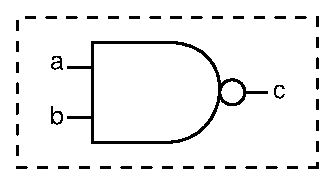
\includegraphics[scale=0.5]{nand2}
&
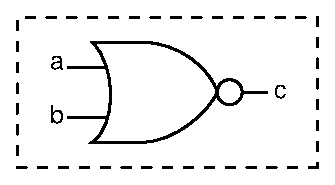
\includegraphics[scale=0.5]{nor2}
\\
\begin{minipage}[b]{2.5in}
\begin{ocamllisting}
class nand2 =
object
   inherit two_input_gate
   method compute_value = not (a && b)
end
\end{ocamllisting}
\end{minipage}
&
\begin{minipage}[b]{2.5in}
\begin{ocamllisting}
class nor2 =
object
   inherit two_input_gate
   method compute_value = not (a || b)
end
\end{ocamllisting}
\end{minipage}
\end{tabular}
\end{center}
%
\begin{enumerate}
\item 
Fill in the definitions of the methods \hbox{\lstinline/connect_input_a/} and \hbox{\lstinline/connect_input_b/}.

\begin{answer}\ifanswers
For the methods \hbox{\lstinline/connect_input_a/} we need to construct a terminal object
that performs the appropriate action.
\begin{ocaml}
   method connect_input_a (wire : wire) =
       wire#add_terminal (object method set x = self#set_input_a x end)
\end{ocaml}
\fi\end{answer}

\item
Define a class \hbox{\lstinline/three_input_gate/} (for gates with three inputs) by inheriting
from \hbox{\lstinline/two_input_gate/}.
\begin{answer}\ifanswers
\begin{ocaml}
class three_input_gate =
object
   inherit two_input_gate
   val mutable c = false
   method private set_input_c x = c <- x; self#set_output
   method connect_input_c (wire : wire) =
       wire#add_terminal (object method set x = self#set_input_c x end)
\end{ocaml}
\fi\end{answer}
   
\item
Would the definition be simpler if the type \hbox{\lstinline/terminal/} were a function instead of an
object (where \hbox{\lstinline/type terminal = bool -> unit/})?

\begin{answer}\ifanswers
It would be slightly simpler because the input terminal could be set without the intermediate terminal object.
The connect methods would have the following form.

\begin{ocaml}
   method connect_input_a (wire : wire) =
      wire#add_terminal self#set_input_a
\end{ocaml}
\fi\end{answer}

\item
What is the purpose of the conditional \hbox{\lstinline/if x <> value then $\cdots$/} in the class \hbox{\lstinline/wire/}?

\begin{answer}\ifanswers
The conditional prevents activity from propagating if it does not change the circuit values.
It also means that the simulation will terminate, even for cyclic circuits, if the circuit becomes quiescent.
\fi\end{answer}

\item
Write a program for the following circuit, called a \emph{SR latch}.
\begin{center}
\begin{tabular}{cc}
\begin{tabular}[b]{cc|c}
S & R & Action\\
\hline
0 & 0 & Keep state\\
0 & 1 & $Q = 0$\\
1 & 0 & $Q = 1$\\
1 & 1 & $Q = 0, \overline{Q} = 0$\\
\\
\end{tabular}
&
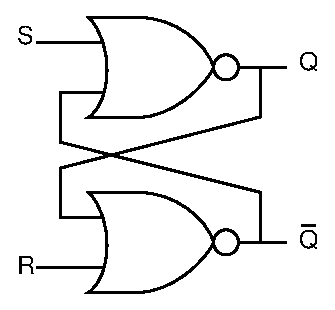
\includegraphics[scale=0.5]{latch}
\end{tabular}
\end{center}

\begin{answer}\ifanswers
\begin{ocaml}
let gate1 = new nor2;;
let gate2 = new nor2;;
let wire1 = new wire;;
let wire2 = new wire;;
gate1#connect_output wire1;;
gate2#connect_output wire2;;
gate1#connect_input_b wire2;;
gate2#connect_input_a wire1;;
\end{ocaml}
\fi\end{answer}
\end{enumerate}
\end{exercise}
   
\begin{exercise}{event-driven-simulator}
The simulator in Exercise~\ref{exercise:circuit-simulation}
has a problem with some cyclic circuits.  For example, the following circuit,
called a \emph{ring oscillator}, oscillates indefinitely, overflowing the stack during simulation.

\begin{center}
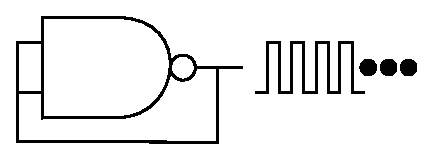
\includegraphics[scale=0.5]{ring}
\end{center}
%
The simulation can be executed in constant stack space by implementing an \emph{event-driven
simulator}.  In the circuit context, an \emph{event} occurs whenever the value on a terminal is set.
An event-driven simulator uses a scheduler to manage events.  When the value of a terminal is set,
the terminal is scheduled, but not executed yet.  When scheduled, the terminal is removed from the
scheduling queue and executed.

Define an event driven simulator by implementing a scheduler.  You can use a scheduling policy of
your choice, but it should be fair, meaning that if a terminal is scheduled, it will eventually be
executed.  

The scheduler should include a method \hbox{\lstinline/main : unit/} that runs until there are no more
events (perhaps forever).  The type \hbox{\lstinline/terminal/} should be defined as follows.
The method \hbox{\lstinline/set/} schedules the terminal, and the method \hbox{\lstinline/execute/} executes it.

\begin{ocaml}
type terminal = < set : bool -> unit; execute : unit >
\end{ocaml}

\begin{answer}\ifanswers
The scheduling queue can be implemented using the \hbox{\lstinline/Queue/} standard library.
This will use a FIFO policy, which is fair.

The scheduler has two methods.  The method \hbox{\lstinline/main/} runs the simulation until the
queue is empty.  The method \hbox{\lstinline/connect_input/} takes a wire and a function, creates
a terminal object, and add the object to the wire.  When the terminal is set, it gets
added to the scheduling queue.  Note that the field \hbox{\lstinline/event_queue/} is accessible
in the inner terminal object.

\begin{ocaml}
type terminal = < set : bool -> unit; execute : unit >

class scheduler =
object (self : 'self)
   val event_queue : terminal Queue.t = Queue.create ()

   method main =
       while not (Queue.is_empty event_queue) do
          (Queue.take event_queue)#execute
       done
   method connect_input (wire : wire) (f : bool -> unit) =
      let term =
         object (term_self)
            val mutable value = false
            method set x =
               value <- x;
               Queue.add term_self event_queue
            method execute = f value
         end
      in
      wire#add_terminal term
end;;

let the_scheduler = new scheduler;;
\end{ocaml}
%
The only other change to the simulation is to the methods \hbox{\lstinline/connect_input_?/}.

\begin{ocaml}
class virtual two_input_gate =
object (self : 'self)
   inherit gate
   val mutable a = false
   val mutable b = false
   method private set_input_a x = a <- x; self#set_output
   method private set_input_b x = b <- x; self#set_output
   method connect_input_a (wire : wire) =
      the_scheduler#connect_input wire self#set_input_a
   method connect_input_b (wire : wire) =
      the_scheduler#connect_input wire self#set_input_b
end
\end{ocaml}
\fi\end{answer}
\end{exercise}

% -*-
% Local Variables:
% Mode: LaTeX
% fill-column: 100
% TeX-master: "paper"
% TeX-command-default: "LaTeX/dvips Interactive"
% End:
% -*-
% vim:tw=100:fo=tcq:

\labelchapter{multiple-inheritance}{Multiple inheritance}

\index{classes!multiple inheritance}
Multiple inheritance is the ability to inherit from more than one superclass.  In OCaml, the
mechanism is simple, any class that contains more than one \hbox{\lstinline/inherit/} directive inherits
from each of them.

Object-oriented programming has received much attention over the years, and multiple inheritance is
one of the more controversial areas.  Some claims against it are that it is complicated, that it
requires extensive training to understand, or that all of its useful features can be captured with
interfaces.  Many of these claims are baloney---in fact, multiple inheritance is often one of the
simplest and most elegant way to combine features and abstractions.  However, there are two main
issues that give rise to these claims:

\begin{itemize}
\item \emph{shadowing}: what happens when two ancestor classes define a method with the same name?
\item \emph{repeated inheritance}: what happens when a class is inherited more than once?
\end{itemize}
%
As we will see, OCaml's model of inheritance is quite simple.  It is essentially equivalent to
textual inclusion, and shadowing follows the normal rule: if a method is defined more than once, the
last definition wins.  First though, let's turn to some examples.

\section{Examples of multiple inheritance}

Multiple inheritance arises whenever an object is described as a collection of features.  Examples
in the real world abound.

\begin{itemize}
\item A \emph{clock radio} is a \emph{timepiece} and a \emph{radio}.
\item An \emph{ambulance} is a \emph{vehicle} and an \emph{emergency medical facility}.
\item A \emph{mobile home} is a \emph{vehicle} and a \emph{home}.
\item A \emph{spork} is a \emph{spoon} and a \emph{fork}.
\item A \emph{graduate student} is a \emph{graduate} and a \emph{student}.
\item A \emph{Swiss army knife} is a \emph{knife} and \emph{scissors} and \emph{pliers} and a \emph{screwdriver} and...
\end{itemize}
%
If we consider these examples, there are really two kinds of combinations: those of independent
features like \emph{clock} and \emph{radio}; and those of related features.  For example, spoons and forks are
both utensils, graduates and students are kinds of persons, \emph{etc}.

\subsection{Inheriting from multiple independent classes}

From a programming perspective, inheritance from independent classes is simpler.  When the classes
to be combined use disjoint names, the result of combining them is simply to produce an object with
all the parts.  For example, consider the following sketches of the classes \hbox{\lstinline/clock/}
and \hbox{\lstinline/radio/}.

\begin{ocaml}
class clock =
object
   val mutable now = $\cdots$
   method gettimeofday = now
   method private tick = $\cdots$
end;;

class radio =
object
   val mutable frequency = 89.3e6
   val mutable volume = 11.0
   method tune freq = $\cdots$; frequency <- freq
   method set_volume vol = $\cdots$; volume <- vol
end;;
\end{ocaml}
%
The combined class \hbox{\lstinline/clock_radio/} simply inherits from both.  The resulting class has the
methods and fields of both superclasses.

\begin{ocaml}
# class clock_radio =
  object
     inherit clock
     inherit radio
  end;;
@
\begin{topoutput}
class clock_radio :
  object
    val mutable frequency : float
    val mutable now : float
    val mutable volume : float
    method gettimeofday : float
    method set_volume : float -> unit
    method private tick : unit
    method tune : float -> unit
  end
\end{topoutput}
@
\end{ocaml}

\subsection{Inheriting from multiple virtual classes}

Sometimes inheritance is used as a mechanism to add functionality by inheriting from a partially
virtual superclass.  Let's take a look at an example, based on the class \hbox{\lstinline/comparable/} we
introduced on page~\pageref{page:comparable}.  We'll define two virtual classes.

\begin{itemize}
\item A \hbox{\lstinline/comparable/} value can be compared to values of the same type.
\item \lstinline/number/ is a class of numbers that can be compared, having a zero, and a negation function.
\end{itemize}
%
The virtual class \hbox{\lstinline/comparable/} declares a virtual method \hbox{\lstinline/compare/}, and derives a
method \hbox{\lstinline/less_than/} from it.

\begin{ocaml}
(* less-than: negative; equal: zero; greater-than: positive *)
type comparison = int

class virtual comparable =
object (self : 'self)
   method virtual compare : 'self -> comparison
   method less_than (x : 'self) = compare self x < 0
end;;
\end{ocaml}
%
For the class \hbox{\lstinline/number/}, we require that the subclass provide
methods \hbox{\lstinline/zero/}, \hbox{\lstinline/neg/} (negate), and \hbox{\lstinline/compare/}.  From that, a
method \hbox{\lstinline/abs/} (absolute value) can be derived.

\begin{ocaml}
class virtual number =
object (self : 'self)
   method virtual zero : 'self
   method virtual neg : 'self
   method virtual compare : 'self -> comparison
   method abs =
      if self#compare self#zero < 0 then
         self#neg
      else
         self
end;;
\end{ocaml}
%
Finally, an actual concrete class of numbers inherits from both classes \hbox{\lstinline/comparable/}
and \hbox{\lstinline/number/}, implementing the virtual methods, and inheriting the derived methods.  The
following class also implements the methods \hbox{\lstinline/less_than/} and \hbox{\lstinline/abs/}
because it inherits them from the virtual superclasses.

\begin{ocaml}
class float_number x =
object (self : 'self)
   inherit comparable
   inherit number

   val number = x
   method representation = number
   method zero = {< number = 0.0 >}
   method neg = {< number = -. number >}
   method compare y = Pervasives.compare x y#representation
end;;
\end{ocaml}

\subsection{Mixins}

\index{mixins}
\index{classes!mixins}
\index{Steve's Ice Cream Parlor}
A \emph{mixin} is a class that is used to add augment the functionality of or
change the behavior of a subclass, but there is no explicit is-a relationship.  According to
folklore, the term mix-in was inspired by Steve's Ice Cream Parlor in Somerville, Massachusetts,
where extra items like nuts, chocolate sprinkles, \emph{etc}., were mixed into a base flavor of ice
cream like chocolate or vanilla.

Let's implement some ice cream with two arbitrary mixed-in flavors.  We'll use the drawable objects
of Chapter~\ref{chapter:objects1}.  A \hbox{\lstinline/blob/} is an object that can be drawn,
including the classes \hbox{\lstinline/circle/} and \hbox{\lstinline/poly/}, and a \hbox{\lstinline/collection/}
is a collection of blobs.

\begin{ocaml}
class vanilla_ice_cream = object $\cdots$ end

class virtual mixed_ice_cream =
object (self)
   inherit vanilla_ice_cream
   inherit collection

   method virtual mixin1 : unit
   method virtual mixin2 : unit

   method stir = self#map (fun item ->
      let t = recenter ** transform#new_rotate (Random.float 6.28)
         ** transform#new_translate (Random.float 10.) (sqrt (Random.float 1e4))
      in item#transform t)

   initializer self#mixin1; self#mixin2; self#stir
end
\end{ocaml}
%
Vanilla ice cream is featureless, but the mixed ice cream contains a collection of extra items.  The
virtual methods \hbox{\lstinline/mixin1/} and \hbox{\lstinline/mixin2/} add the extra items to the collection.  To
implement a particular kind of mixed ice cream, we implement two classes, one for each mixin.

\begin{ocaml}
class drop = circle ~color:0x880022 (0., 0.) 10.
class sprinkle = poly ~color:0x220044 [|(0., 0.); (10., 0.); (10., 3.); (0., 3.)|]

class virtual drop_mixin1 =
object (self)
   method virtual add : blob -> unit
   method mixin1 = for i = 0 to 4 do self#add (new drop) done
end

class virtual sprinkle_mixin2 =
object (self)
   method virtual add : blob -> unit
   method mixin2 = for i = 0 to 200 do self#add (new sprinkle) done
end
\end{ocaml}
%
For the final product, we just mix the ice cream with its ingredients.
The mixin classes implement the virtual methods of the ice cream class,
and the result is a flavored ice cream.

\begin{ocaml}
class my_favorite_ice_cream =
object
   inherit mixed_ice_cream
   inherit drop_mixin1
   inherit sprinkle_mixin2
end
\end{ocaml}
%
This use of inheritance is not a specialization.  We certainly don't mean
that \hbox{\lstinline/my_favorite_ice_cream/} is-a \hbox{\lstinline/sprinkle/}, or a collection of sprinkles, or
anything of the sort.  The purpose of the inheritance in this case is simply for the mixin to
specify an item that is to be added to the ice cream.

\begin{center}
\begin{tabular}{ll}
\begin{minipage}[b]{2in}
\begin{ocamllisting}
(new my_favorite_ice_cream)#draw;;
\end{ocamllisting}
\end{minipage}
&
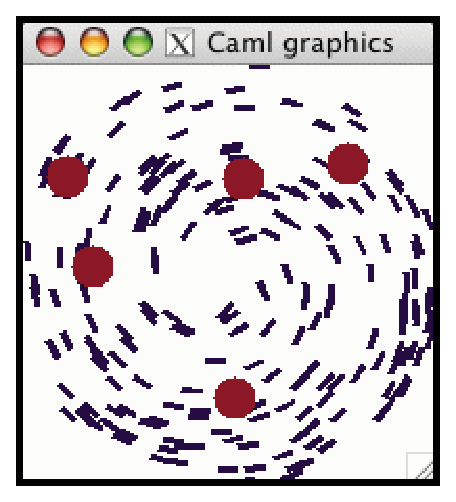
\includegraphics[scale=0.3]{ice_cream}
\end{tabular}
\end{center}
%
In all the examples of this section, the inheritance is used to combine classes that are
really independent.  In each case, there may be several declarations of a method as virtual, but there only
one implementation.  Let's turn to the more general case where methods and fields may be defined
multiple times, starting with the topic of \emph{shadowing}.

\section{Overriding and shadowing}

What happens when an object defines a name twice?  For comparison, let's first consider a similar
question: what happens in a module when a name is defined twice?  We know the answer---the
definition exported by the module is the last one.

\begin{ocaml}
# module M =
  struct
     let x = 1;;
     Printf.printf "x = %d!\n" x;;
     let x = 2;;
  end;;
@
\begin{topoutput}
x = 1!
\end{topoutput}
@
# M.x;;
@
\begin{topoutput}
- : int = 2
\end{topoutput}
@
\end{ocaml}
%
Objects are a little different from modules, but the naming is similar.  Consider the following
objects that contain duplicate definitions.  OCaml warns about the duplication, but it is
instructive to see the results.  First, let's override a method.

\begin{ocaml}
# let a =
  object
     method get = 1
     method get = 2
  end;;
@
\begin{topoutput}
Warning M: the method get is overriden in the same class.
val a : < get : int > = <obj>
\end{topoutput}
@
# a#get;;
- : int = 2
\end{ocaml}
%
As would be expected, the last method definition is the one that is used by the object.
We can try the same thing with fields.

\begin{ocaml}
# let b =
  object
     val x = 1
     method get = x
     val x = 2
  end;;
@
\begin{topoutput}
Warning V: the instance variable x is overriden.
\end{topoutput}
@
# b#get;;
@
\begin{topoutput}
- : int = 2
\end{topoutput}
@
\end{ocaml}
%
Field override seems to be frowned upon by the compiler.  Still, the result is the same, it is the
last definition that is used by the object.  Any preceding definitions for the same name are
ignored.

\section{Repeated inheritance}
\index{inheritance!repeated}
\index{inheritance!diamond problem}
\index{classes!repeated inheritance}
\index{classes!diamond problem}

Repeated inheritance occurs when a class inherits from another along multiple paths in the
inheritance hierarchy, perhaps more commonly known as the ``diamond problem.''  For example, we
might say that a French programmer is both French and a programmer, and both of these are more
generally persons.  That means that a French programmer inherits from person twice.  The following
diagram illustrates the class relationship, with a hypothetical programmer in italics.

\begin{center}
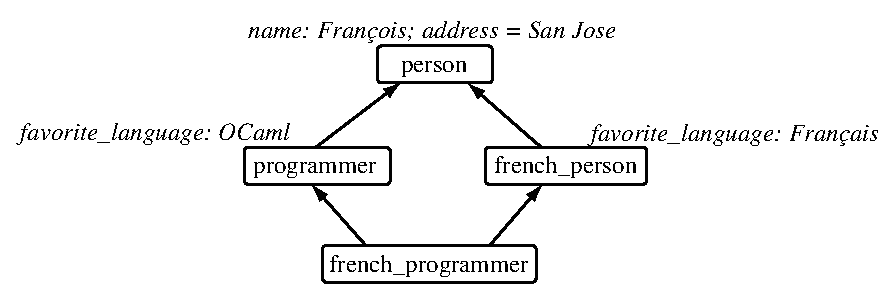
\includegraphics[scale=0.75]{french-programmer}
\end{center}
%
In OCaml, the \hbox{\lstinline/inherit/} directive is nearly equivalent to textual inclusion---the result
is the same as if the \hbox{\lstinline/inherit/} clause were replaced with the text of the class being
inherited from.  This means that a \hbox{\lstinline/programmer/} includes the program text for
a \hbox{\lstinline/person/}, so does a \hbox{\lstinline/french_person/}, and the \hbox{\lstinline/french_programmer/}
contains the program text twice.

When does this make a difference?  For any given method or field, remember the rule: it is
the \emph{last} definition that matters, so perform the textual expansion mentally and look for the
final definition.  Consider a case where a class \hbox{\lstinline/a/} is inherited twice.

\begin{ocamlnum}
# class a =
  object
     method x = 1
  end;;
# class b =
  object
     inherit a
     method x = 2
     inherit a
  end;;
@
\begin{topoutput}
Warning: ... x ... is overriden by the class a
\end{topoutput}
@
# (new b)#x;;
@
\begin{topoutput}
- : int = 1
\end{topoutput}
@
\end{ocamlnum}
%
The result is \hbox{\lstinline/1/} because the final definition for the method \hbox{\lstinline/x/} comes from the
inherit clause on line 9 (which defines \hbox{\lstinline/x/} as \hbox{\lstinline/1/}).

The diamond problem is similar.  Consider the French programmer example, here
drawn in the shape of a diamond (don't type it in this way).

\begin{center}
\begin{minipage}{4in}
\begin{ocamllisting}
                      class person =
                      object
                          method name = "Francois"
                          method address = "San Jose"
                      end

class programmer =                     class french_person =
object                                 object
   inherit person                         inherit person
   method lang = "OCaml"                  method lang = "Francais"
end                                    end

                      class french_programmer =
                      object
                          inherit programmer
                          inherit french_person
                      end
\end{ocamllisting}
\end{minipage}
\end{center}
%
Let's think how the text will be expanded for class \hbox{\lstinline/french_programmer/}.  If we perform the expansion,
here is the order in which the methods are defined:
\hbox{\lstinline/person#name,address/}, \hbox{\lstinline/programmer#lang/}, \hbox{\lstinline/person#name,address/}, \hbox{\lstinline/french_person#lang/}.
Keeping only the final definition for each method, we obtain the following class,
equivalent to \hbox{\lstinline/french_programmer/}.

\begin{ocaml}
class french_programmer_flattened =
object
   method name = "Francois"
   method lang = "Francais"
   method address = "San Jose"
end
\end{ocaml}
%
Field override works the same as method override for fields that are visible.  If we had defined the
values as fields instead of methods, the result would be the same: the
favorite language is Fran\c{c}ais.

However, fields that are hidden (because of typing) are not overridden; they are duplicated.
Suppose we define a class \hbox{\lstinline/a/} that defines a mutable field \hbox{\lstinline/x/}, which is then
hidden using a type constraint.

\begin{ocaml}
class type a_type =
object
   method set : int -> unit
   method get : int
end;;

class a : a_type =
object
   val mutable x = 0
   method set y = x <- y
   method get = x
end;;
\end{ocaml}
%
Repeated inheritance \emph{duplicates} the hidden field \hbox{\lstinline/x/}, which means that operations
on one copy of \hbox{\lstinline/a/} do not effect the others.

\begin{ocaml}
# class b =
  object
     inherit a as super1
     inherit a as super2

     method test =
        super1#set 10;
        super2#get
  end;;
@
\begin{topoutput}
class b :
  object method get : int method set : int -> unit method test : int end
\end{topoutput}
@
# (new b)#test;;
@
\begin{topoutput}
- : int = 0
\end{topoutput}
@
\end{ocaml}

\section{Avoiding repeated inheritance}

The previous section points out the issue with multiple inheritance, which is that there
are at least two different policies for repeated inheritance: override and copying.
There is no single policy that is best.  For example, the French programmer
may wish to go by the same name in all contexts, but he might wish to use a different address for
his occupation than he uses as a French citizen.  That is, the repeated field \hbox{\lstinline/name/}
should refer to the same value, but the \hbox{\lstinline/address/} field should be copied.

As pointed out, OCaml uses the following policy: visible fields and methods use the override policy,
fields and methods that are hidden use the copy policy.  This policy can be difficult for a
programmer to adhere to, ``All the fields that are hidden are copied.''  The semantics of multiple
inheritance might be simple enough to state, ``it is just textual expansion,'' but the problem is
that it might be necessary to know the text of all repeated superclasses.  For this reason and
others, it is natural to want to avoid repeated inheritance, at least in some cases.

\subsection{Is-a \emph{vs}.{} has-a}

For an example, suppose we have classified vehicles in two different ways: according to where they
are used, and by how they are powered.  In the following diagram, the class \hbox{\lstinline/vehicle/} is a
superclass of all the others; for example it might contain methods to move forward or
stop, \emph{etc}.  A \hbox{\lstinline/car/} is a vehicle that travels roads, a \hbox{\lstinline/boat/} water;
an \hbox{\lstinline/electric_vehicle/} needs to be charged occasionally, \emph{etc}.

\begin{center}
\begin{tabular}{|c|c|}
\hline
\multicolumn{2}{|c|}{\hbox{\lstinline/vehicle/}}\\
\hline
\hbox{\lstinline/car/} & \hbox{\lstinline/electric_vehicle/}\\
\hbox{\lstinline/boat/} & \hbox{\lstinline/gasoline_vehicle/}\\
\hbox{\lstinline/submarine/} & \hbox{\lstinline/rocket/}\\
\hbox{\lstinline/spacecraft/} & \hbox{\lstinline/pedaled_vehicle/}\\
& \hbox{\lstinline/sailed_vehicle/}\\
& \hbox{\lstinline/nuclear_vehicle/}\\
\hline
\end{tabular}
\end{center}
%
A particular kind of vehicle can constructed by combining a property from the left column and
another from the right.  We have gasoline powered boats, nuclear submarines, and electric cars.
Some combinations don't make much sense, like pedaled spacecraft.

On the surface, this classification may seem reasonable.  We classify vehicles by two
orthogonal properties, and use multiple inheritance to define classes for the combinations that make
sense.  However, this will involve repeated inheritance, which might be a problem if we don't know how
the class \hbox{\lstinline/vehicle/} is defined.

There is another way to classify vehicles that is just as natural, but avoids the repeated
inheritance.  That is, we can continue to classify vehicles by where they travel, but instead of
classifying powered vehicles, we classify power sources directly.

\begin{center}
\begin{tabular}{lr}
\begin{tabular}[t]{|c|}
\hline
\hbox{\lstinline/vehicle/}\\
\hline
\hbox{\lstinline/car/}\\
\hbox{\lstinline/boat/}\\
\hbox{\lstinline/submarine/}\\
\hbox{\lstinline/spacecraft/}\\
\hline
\end{tabular}
&
\begin{tabular}[t]{|c|}
\hline
\hbox{\lstinline/power_source/}\\
\hline
\hbox{\lstinline/electric_motor/}\\
\hbox{\lstinline/gasoline_engine/}\\
\hbox{\lstinline/rocket_engine/}\\
\hbox{\lstinline/pedals/}\\
\hbox{\lstinline/sails/}\\
\hbox{\lstinline/nuclear_plant/}\\
\hline
\end{tabular}
\\
\multicolumn{2}{c}{
\begin{tabular}[t]{|c|}
\hline
\hbox{\lstinline/assembled_vehicle/}\\
\hline
\hbox{\lstinline/electric_car = car + electric_motor/}\\
\hbox{\lstinline/nuclear_submarine = submarine + nuclear_plant/}\\
\hbox{\lstinline/sailboat = boat + sails/}\\
\hbox{\lstinline/rocket = spacecraft + rocket_engine/}\\
$\cdots$\\
\hline
\end{tabular}}
\end{tabular}
\end{center}
%
Now we have two independent concepts, vehicles and power sources, and an assembled vehicle needs one
of each.  The assemblies can be created with multiple inheritance, which has the advantage that
bogus assemblies (like rocket-powered submarines) can be omitted from the collection.

An alternative to multiple inheritance is for the vehicle class to take a power source as an
argument and include it as a field.  There are two potential advantages.  One is
that it is not necessary to write down every possible assembly.  The other is that it might make
more sense semantically---a vehicle has-a power source, but it isn't-a power source, at least not
normally.  A disadvantage is that it isn't easy to rule out combinations that don't make sense.

\subsection{Mixins revisited}

In many ways, the approach to the vehicle example is really just a mixin.  Power sources aren't
really useful until they are harnessed, which happens when an assembled vehicle is created by mixing
in a power source into a vehicle.

This suggests that one approach to avoiding repeated inheritance is to delay the use of multiple
inheritance as much as possible.  Returning to the French programmer, there were four classes with a
repeated base class \hbox{\lstinline/person/}.  Another way to design the hierarchy is to partition the
properties, where the programming and French properties are split from the \hbox{\lstinline/person/} and
become mixins.

\begin{center}
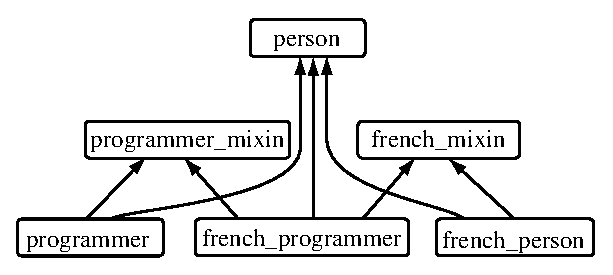
\includegraphics[scale=0.75]{french-mixin}
\end{center}
%
The mixin classes \hbox{\lstinline/programmer_mixin/} and \hbox{\lstinline/french_mixin/} are now standalone
classes.  They can still refer to the properties of being a person through virtual methods and fields, but they
don't make much sense alone until combined with the \hbox{\lstinline/person/} class.

As with any programming style, it isn't always appropriate to program this way.  There are more
classes; the relationship between classes is not as well defined---there is nothing that says that
a \hbox{\lstinline/programmer_mixin/} is to be combined with a \hbox{\lstinline/person/}; and it is easy to forget
about maintaining the relationship between a class and its mixins.  Of course, in many cases
this \emph{is} a useful technique, and it can lead to simpler, shorter programs.

At this point we have covered objects, classes with single inheritance, and classes with multiple
inheritance.  The object system is quite powerful, and we have many tools at our disposal.  There is
one remaining important topic: polymorphic classes, which we discuss in the next chapter.

% -*-
% Local Variables:
% Mode: LaTeX
% fill-column: 100
% TeX-master: "paper"
% TeX-command-default: "LaTeX/dvips Interactive"
% End:
% -*-
% vim:tw=100:fo=tcq:

\exercises

%%%%%%%%%%%%%%%%%%%%%%%%%%%%%%%%%%%%%%%%%%%%%%%%%%%%%%%%%%%%%%%%%%%%%%%%
% Names
%
\begin{exercise}{person-name}
Assume there is a class \hbox{\lstinline/name/} that represents the
name of a person.  We would normally say that a \hbox{\lstinline/person/} is-a \hbox{\lstinline/human/} and has-a \hbox{\lstinline/name/},

\begin{ocaml}
class person (n : name) = object inherit human val name = n $\cdots$ end
\end{ocaml}
%
Suppose that instead, the class \hbox{\lstinline/person/} inherits from both.

\begin{ocaml}
class person (s : string) =
object
   inherit human
   inherit name s
   $\cdots$
end
\end{ocaml}
%
What is the difference?  Under what conditions would the different
representations be preferred?

\begin{answer}\ifanswers
In the former case, a person is not a name, and can't be used as a
name.  With multiple inheritance, the person \emph{can} be used as a
name.  Multiple inheritance is more likely to be used in a situation
where the name of a person and the person himself are treated as the
same thing.  The former is more likely when the name is just a symbol
for the person.
\fi\end{answer}
\end{exercise}

%%%%%%%%%%%%%%%%%%%%%%%%%%%%%%%%%%%%%%%%%%%%%%%%%%%%%%%%%%%%%%%%%%%%%%%%
% Reference counting
%
\begin{exercise}{reference-counting}
Consider the following class, which implements a persistent
reference-counted value stored in a file.  When there are no more
references, the file is removed.

\begin{ocaml}
class persistent_refcounted_value filename =
object (self)
    (* persistent_value *)
    val mutable x : int list =
       let fin = open_in_bin filename in
       let x = input_value fin in
       close_in fin;
       x
    method get = x
    method set y = x <- y; self#save
    method private save =
       let fout = open_out_bin filename in
       output_value fout x;
       close_out fout

    (* refcounted_value *)
    val mutable ref_count = 1
    method add_ref = ref_count <- ref_count + 1
    method rm_ref =
       ref_count <- ref_count - 1;
       if ref_count = 0 then
          Sys.remove filename
end
\end{ocaml}
%
\begin{enumerate}
\item Partition the class into three classes: \hbox{\lstinline/persistent_value/} implements
persistent values stored in files, \hbox{\lstinline/refcounted_value/} implements generic reference
counted objects, and \hbox{\lstinline/persistent_refcounted_value/} inherits from both.

\item What is the advantage in partitioning the class?
\end{enumerate}

\begin{answer}\ifanswers
\begin{enumerate}
\item
The class is simply split down the middle.  The details of deletion must be implemented by
the value, not the reference counting class, so the virtual method \hbox{\lstinline/delete/} is
used to connect the two objects.

\begin{ocaml}
class persistent_value filename =
object (self)
    val mutable x : int list =
       let fin = open_in_bin filename in
       let x = input_value fin in
       close_in fin;
       x
    method get = x
    method set y = x <- y; self#save
    method private save =
       let fout = open_out_bin filename in
       output_value fout x;
       close_out fout
    method private delete = Sys.remove filename
end

class virtual ref_value =
object (self)
    val mutable ref_count = 1
    method add_ref = ref_count <- ref_count + 1
    method rm_ref =
       ref_count <- ref_count - 1;
       if ref_count = 0 then self#delete
    method private virtual delete : unit
end

class persistent_ref_value2 filename =
object
   inherit persistent_value filename
   inherit ref_value
end
\end{ocaml}

\item The advantage of splitting the class is that we now have two more generic classes.
For example, reference counting is general concept that can be re-used elsewhere in the program.
\end{enumerate}
\fi\end{answer}
\end{exercise}

%%%%%%%%%%%%%%%%%%%%%%%%%%%%%%%%%%%%%%%%%%%%%%%%%%%%%%%%%%%%%%%%%%%%%%%%
% Programmer
%
\begin{exercise}{french-programmer}
In the French programmer example, the \hbox{\lstinline/programmer/} has a
field \hbox{\lstinline/favorite_language/} and so does
the \hbox{\lstinline/french_person/}.  Can the inheritance hierarchy be
modified so that these are available
as \hbox{\lstinline/favorite_programming_language/}
and \hbox{\lstinline/favorite_natural_language/}, without
modifying the classes \hbox{\lstinline/programmer/} and \hbox{\lstinline/french_person/}?

\begin{answer}\ifanswers
OCaml doesn't provide a way to rename fields, so the only thing we can
do is to hide the field and use methods to access it.  Suppose the
class \hbox{\lstinline/programmer/} is defined as follows.

\begin{ocaml}
class programmer =
object
   inherit person
   val favorite_language = "OCaml"
end
\end{ocaml}
%
The renamed class \hbox{\lstinline/programmer'/} could be defined as follows.

\begin{ocaml}
class type programmer_type' =
object
   val name : string
   val address : string
   method favorite_programming_language : string
end

class programmer' : programmer_type' =
object
   inherit programmer
   method favorite_programming_language = favorite_language
end
\end{ocaml}
\fi\end{answer}
\end{exercise}

%%%%%%%%%%%%%%%%%%%%%%%%%%%%%%%%%%%%%%%%%%%%%%%%%%%%%%%%%%%%%%%%%%%%%%%%
% Lists
%
\begin{exercise}{multiple-list}
You are given the following functor that defines a class \hbox{\lstinline/cell/}
containing a value of type \hbox{\lstinline/T.t/}.

\begin{ocaml}
module MakeCell (T : sig type t end) =
struct
    class cell x =
    object
        val mutable x : T.t = x
        method private get = x
        method private set y = x <- y
    end
end
\end{ocaml}
%
Define a singly-linked list of integers by inheriting from the class \hbox{\lstinline/cell/}
twice.  Your class should have the type \hbox{\lstinline/int_cons/}.

\begin{ocaml}
class type int_cons =
object
   method hd : int
   method tl : int_cons option
   method set_hd : int -> unit
   method set_tl : int_cons option -> unit
end

type int_list = int_cons option
\end{ocaml}

\begin{answer}\ifanswers
Inheriting from the \hbox{\lstinline/cell/} twice would override the
methods \hbox{\lstinline/get/} and \hbox{\lstinline/set/}, which is not what we
want.  We need to \emph{rename} the methods first.  For this list, it
is sufficient to rename the methods in just one of the classes.  Note
that the cell value is hidden so that it is not overridden.

\begin{ocaml}
module IntCell =
struct
   module Cell = MakeCell (struct type t = int end);;

   class type cell_type =
   object
      method private get_int : int
      method private set_int : int -> unit
   end

   class cell i : cell_type =
   object (self)
      inherit Cell.cell i
      method private get_int = self#get
      method private set_int = self#set
   end
end

module ListCell = MakeCell (struct type t = int_list end);;

class cons i : int_cons =
object
    inherit IntCell.cell i as value
    inherit ListCell.cell None as link

    method hd = value#get_int
    method tl = link#get
    method set_hd = value#set_int
    method set_tl = link#set
end
\end{ocaml}
\fi\end{answer}
\end{exercise}    
    
%%%%%%%%%%%%%%%%%%%%%%%%%%%%%%%%%%%%%%%%%%%%%%%%%%%%%%%%%%%%%%%%%%%%%%%%
% Recursive functions
%
\begin{exercise}{multiple-recursive-functions}
Suppose we have several mutually-recursive functions 
\hbox{\lstinline/$f_1$ : int -> int/}, $\ldots$, \hbox{\lstinline/$f_n$ : int -> int/}
that we want to define in separate files.  In
Exercise~\ref{exercise:functor5} we did this with recursive modules.
Do it with multiple inheritance instead.  Is there any advantage to
using classes over recursive modules?

\begin{answer}\ifanswers
Each function $f_i : int -> int$ would be defined in a separate class,
where all the other functions are virtual.

\begin{ocaml}
class virtual fun_$i$ =
object
   method virtual $f_1$ : int -> int
   $\cdots$
   method virtual $f_{i - 1}$ : int -> int
   method $f_i$ i = $\cdots$
   $\cdots$
   method virtual $f_n$ : int -> int
end
\end{ocaml}
%
The final class would use multiple inheritance to tie the recursive knot.
%
\begin{ocaml}
class everything =
object
   inherit fun_$1$ $\cdots$ inherit fun_$n$
end
\end{ocaml}
%
To reduce the amount of code, a single shared base class could be used
to declare all the functions.

\begin{ocaml}
class virtual declarations =
object
   method virtual $f_1$ : int -> int
   $\cdots$
   method virtual $f_n$ : int -> int
end

class virtual fun_$i$ =
object
   inherit declarations
   method $f_i$ i = $\cdots$
end
\end{ocaml}
%
An advantage of the class representation is that the text required
for the declarations is \emph{much} smaller than needed for recursive
modules.
\fi\end{answer}
\end{exercise}

% -*-
% Local Variables:
% Mode: LaTeX
% fill-column: 100
% TeX-master: "paper"
% TeX-command-default: "LaTeX/dvips Interactive"
% End:
% -*-
% vim:tw=100:fo=tcq:

%
%
%

\labelchapter{polyclasses}{Polymorphic Classes}
\index{classes!polymorphic}

So far, we have seen many kinds of class and class type definitions.  Classes can be fixed, or they
can be parameterized by ordinary values.  In addition, classes and class types can be
\emph{polymorphic}, meaning that they can be parameterized by types, just like other expressions and
types in the language (except for module types).

This kind of generic object-oriented programming appears in other
programming languages in various forms.  The Eiffel programming
language supports \emph{genericity}; C++ has a construct
called \emph{templates}; Java has type-parameterized classes
called \emph{generics}.

In OCaml, polymorphism is not a new concept when applied to classes.
It is the \emph{same} concept that appears throughout the language,
and it works the same way for classes and class types as it does for
other constructs.

\labelsection{poly-map}{Polymorphic dictionaries}
\label{page:poly-map}
\label{classes:polymorphic}

Let's start with an example based on the ``map'' data structure that
we developed in Section~\reflabelsection{module-reuse}
using functors.  A map is a
dictionary containing key-value pairs, parameterized by a
function \hbox{\lstinline$compare$} that defines a total order on keys.  For
brevity, we'll implement the map using association lists.

\begin{ocaml}
# type ordering = Smaller | Equal | Larger
@
\begin{topoutput}
type ordering = Smaller | Equal | Larger
\end{topoutput}
@
# class ['key, 'value] map (compare : 'key -> 'key -> ordering) =
     let equal key1 (key2, _) = compare key1 key2 = Equal in
     object (self : 'self)
        val elements : ('key * 'value) list = []
        method add key value = {< elements = (key, value) :: elements >}
        method find key = snd (List.find (equal key) elements)
     end;;
@
\begin{topoutput}
class ['a, 'b] map : ('a -> 'a -> ordering) ->
  object ('self)
    val elements : ('a * 'b) list
    method add : 'a -> 'b -> 'self
    method find : 'a -> 'b
  end
\end{topoutput}
@
\end{ocaml}
%
The result type has been edited slightly for readability.

The class definition is parameterized by two types, \hbox{\lstinline$'key$}
and \hbox{\lstinline$'value$}, written within square brackets before the
class name as \hbox{\lstinline$['key, 'value]$}.  The square brackets are
required even if there is only one type parameter to a class definition.

The entries of the map are stored in the list \hbox{\lstinline$elements$}, of
type \hbox{\lstinline$('key * 'value) list$}, and the map's methods examine
the list.  This implementation of a map is pure, the
method \hbox{\lstinline$add$} produces a new object with the new entry added
to the list, leaving the \hbox{\lstinline$self$} object unchanged.

\labelsubsection{polyclasses-type-constraints}{Free type variables in polymorphic classes}
\index{classes!free type variables}

The type constraints, besides being good documentation, are required.
Class definitions are not allowed to have free type variables, meaning
that every type variable must be a parameter, or it must be bound
somewhere else in the class definition.  The following definition
fails.

\begin{ocaml}
# class ['a] is_x x =   (* Does not work! *)
     object (self : 'self)
        method test y = (x = y)
     end;;
@
\begin{toperror}
Some type variables are unbound in this type:
  class ['a] is_x : 'b -> object method test : 'b -> bool end
The method test has type 'a -> bool where 'a is unbound
\end{toperror}
@
\end{ocaml}
%
The reason for the failure is that the type of the
argument \hbox{\lstinline$x$} is not specifically written as being of
type \hbox{\lstinline$'a$}, hence the method \hbox{\lstinline$test$} has some
type \hbox{\lstinline$'b -> bool$}, where the type variable \hbox{\lstinline$'b$} is
not a parameter of the class.  The solution is to constrain the types
so that the method \hbox{\lstinline$test$} has type \hbox{\lstinline$'a -> bool$}.

\begin{ocaml}
# class ['a] is_x (x : 'a) =
     object (self : 'self)
        method test y = (x = y)
     end;;
@
\begin{topoutput}
class ['a] is_x : 'a -> object method test : 'a -> bool end
\end{topoutput}
@
\end{ocaml}

\labelsubsection{poly-instantiation}{Instantiating a polymorphic class}

Instantiating a class (to get an object), works the same it does with
non-polymorphic classes.  The \hbox{\lstinline$new$} operator is used to
instantiate the class.  For example, here is how we might construct an
actual map object where the keys are integers.

\begin{ocaml}
# let compare_int (i : int) (j : int) =
     if i < j then Smaller
     else if i > j then Larger
     else Equal;;
@
\begin{topoutput}
val compare_int : int -> int -> ordering = <fun>
\end{topoutput}
@
# let empty_int_map = new map compare_int;;
@
\begin{topoutput}
val empty_int_map : (int, '_a) map = <obj>
\end{topoutput}
@
# let one = empty_int_map#add 1 "One";;
@
\begin{topoutput}
val one : (int, string) map = <obj>
\end{topoutput}
@
# empty_int_map;;
@
\begin{topoutput}
- : (int, string) map = <obj>
\end{topoutput}
@
\end{ocaml}
%
Note that the type for the empty map is
\hbox{\lstinline$empty_int_map : (int, '_a) map$}.
That is, it does not have polymorphic type, hence it can be used only
at one type.  This is due to the \emph{value
restriction} (Section \reflabelsection{value-restriction})---the
expression \hbox{\lstinline$new map compare_int$} is an application, so it
is not a value, and so it is not polymorphic.
For the most part, the practical consequences of the value restriction
are minimal, it simply means that a new empty map must be created for
each type of map value that is to be used in a program.

One additional step we might take is to define a class specifically for
the case when the keys are integers.  The new class is polymorphic
over just one type, the type of values.

\begin{ocaml}
# class ['value] int_map = [int, 'value] map compare_int;;
@
\begin{topoutput}
class ['a] int_map : [int, 'a] map
\end{topoutput}
@
\end{ocaml}
%
Note that the type arguments are required on the right as part of the
definition (in addition to the normal value
argument \hbox{\lstinline$compare_int$}).  The syntax for type arguments is a
sequence of comma-separated type expressions between square brackets,
placed before the class name.  We could, if we wish, further constrain
the type.

\begin{ocaml}
# class int_map2 = [int, string * float] map compare_int;;
@
\begin{topoutput}
class int_map2 : [int, string * float] map
\end{topoutput}
@
\end{ocaml}

\labelsubsection{poly-inheritance}{Inheriting from a polymorphic class}

Inheriting from a polymorphic class works as usual, except that type arguments
to polymorphic superclasses must be supplied explicitly.  Let's define
a new kind of map that supports a method \hbox{\lstinline$iter$} that applies a function
once to each entry in the map.

\begin{ocaml}
# class ['key, 'value] iter_map compare =
    object
      inherit ['key, 'value] map compare
      method iter f = List.iter (fun (key, value) -> f key value) elements
    end;;
@
\begin{topoutput}
class ['a, 'b] iter_map : ('a -> 'a -> ordering) ->
  object ('c)
    ...
    method iter : ('a -> 'b -> unit) -> unit
  end
\end{topoutput}
@
\end{ocaml}
%
The directive \hbox{\lstinline$inherit$} takes the type arguments in addition
to any normal arguments, but otherwise the directive works as
expected.

Next, let's consider a new method \hbox{\lstinline$map$} that applies a
function to each of the values in the dictionary, returning a new map.  Given
a function \hbox{\lstinline$f : 'value -> 'value2$}, what should be the type
of the method \hbox{\lstinline$map$}?  Let's write the code.

\begin{ocaml}
# class ['key, 'value] map_map compare =
  object (self : 'self)
    inherit ['key, 'value] map compare
    method map f =
      {< elements = List.map (fun (key, value) -> key, f value) elements >}
  end;;
@
\begin{topoutput}
class ['a, 'b] map_map : ('a -> 'a -> ordering) ->
  object ('self)
    ...
    method map : ('b -> 'b) -> 'self
  end
\end{topoutput}
@
\end{ocaml}
%
Note the type of the method \hbox{\lstinline$map$}, which requires that the
function argument have type \hbox{\lstinline$'b -> 'b$}.  We might have
expected a more general typing where, given an object of
type \hbox{\lstinline$obj : ['key, 'value1] map_map$} and a
function \hbox{\lstinline$f : 'value1 -> 'value2$}, that the
expression \hbox{\lstinline$obj#map f$} would have type
\hbox{\lstinline$['key, 'value2] map_map$}.  

There is a good reason for the more restrictive typing.  Suppose we
decide to build a variation on a map where, instead of the
method \hbox{\lstinline$find$} raising an exception when an entry is not
found, it returns some default value.  The new class is easy to
define.

\begin{ocaml}
class ['key, 'value] default_map compare (default : 'value) =
  object (self : 'self)
     inherit ['key, 'value] map_map compare as super
     method find key =
        try super#find key with
           Not_found -> default
  end;;
\end{ocaml}
%
Objects of the class \hbox{\lstinline$default_map$} have two places
where values of type \hbox{\lstinline$'value$} appear: in the list
of \hbox{\lstinline$elements$}, and the \hbox{\lstinline$default$}
value.  It is not safe to change the type
of \hbox{\lstinline$elements$} without also changing
the \hbox{\lstinline$default$} value in the same way.  In this case,
the more general typing for the method \lstinline$map$ would be unsafe
because it doesn't also change the \lstinline$default$ value.

Of course, OCaml does not try to predict how subclasses will be
created.  The only safe approach is for the object type to be
invariant.

\labelsection{polymorphic-class-types}{Polymorphic class types}

Polymorphic classes have polymorphic class types, using the usual
syntax where the type parameters are enclosed in square brackets.

\begin{ocaml}
# class type ['key, 'value] map_type =
    object ('self)
      method add  : 'key -> 'value -> 'self
      method find : 'key -> 'value
    end;;
@
\begin{topoutput}
class type ['a, 'b] map_type =
  object ('c) method add : 'a -> 'b -> 'c method find : 'a -> 'b end
\end{topoutput}
@
# class ['key, 'value] map2 (compare : 'key -> 'key -> ordering)
  : ['key, 'value] map_type =
    let equal key1 (key2, _) = compare key1 key2 = Equal in
    object $\cdots$ end
@
\begin{topoutput}
class ['a, 'b] map2 : ('a -> 'a -> ordering) -> ['a, 'b] map_type
\end{topoutput}
@
\end{ocaml}
%
This implementation of the class \hbox{\lstinline$map2$} is entirely
self-contained.  Let's look at an example of a recursive definition,
based on the implementation of binary search trees in
Section~\reflabelsection{union-binary-trees}.  In that section, we defined
the binary tree with the following polymorphic union type.

\begin{ocaml}
type 'a tree =
   Node of 'a * 'a tree * 'a tree
 | Leaf;;
\end{ocaml}
%
If we wish to take an object-oriented approach, we can implement each
case of the union as a class that has a class type
\hbox{\lstinline$['a] tree$}, where the type \hbox{\lstinline$['a] tree$}
specifies the operations on a tree, but not its implementation.  For
our purposes, a tree supports a functional \hbox{\lstinline$add$} operation
to add an element to the tree, and a \hbox{\lstinline$mem$} function to test
for membership in the tree.

\begin{ocaml}
class type ['a] tree =
  object ('self)
    method add : 'a -> 'a tree
    method mem : 'a -> bool
  end;;
\end{ocaml}
%
\label{page:poly-tree}
There are then two classes that implement a tree: a 
class \hbox{\lstinline$['a] leaf$} 
that represents the empty tree, and a
class \hbox{\lstinline$['a] node$}
that represents an internal node.  Let's start with the internal
node.

\begin{ocaml}
class ['a] node (compare : 'a -> 'a -> ordering)
    (x : 'a) (l : 'a tree) (r : 'a tree) =
  object (self : 'self)
    val label = x
    val left = l
    val right = r
    method mem y =
      match compare y label with
         Smaller -> left#mem y
       | Larger -> right#mem y
       | Equal -> true
    method add y =
      match compare y label with
         Smaller -> {< left = left#add y >}
       | Larger -> {< right = right#add y >}
       | Equal -> self
  end;;
\end{ocaml}
%
An internal node has three fields: a label and two children, where the
children have type \hbox{\lstinline$'a tree$}.  The method \hbox{\lstinline$mem$}
performs a binary search, and the method \hbox{\lstinline$add$} performs a
functional update, returning a new tree.

The class \hbox{\lstinline$['a] leaf$} is simpler, the method \hbox{\lstinline$mem$}
always returns \hbox{\lstinline$false$}, and the method \hbox{\lstinline$add$}
produces a new internal node.

\begin{ocaml}
class ['a] leaf (compare : 'a -> 'a -> ordering) =
  object (self : 'self)
    method mem (_ : 'a) = false
    method add x =
      new node compare x (new leaf compare) (new leaf compare)
  end;;
\end{ocaml}
%
This implementation is adequate, but it is slightly inefficient because
the method \hbox{\lstinline$add$} creates entirely new leaves.  Since all
leaves are the same, we might consider using \hbox{\lstinline$self$} instead,
but we run into a type error because the type \hbox{\lstinline$'self$} is not
equivalent to \hbox{\lstinline$'a tree$}.

\begin{ocaml}
# class ['a] leaf (compare : 'a -> 'a -> ordering) =
    object (self : 'self)
      method mem (_ : 'a) = false
      method add x = new node compare x self self
    end;;
@
\begin{toperror}
Characters 151-155:
        new node compare x self self
                           ^^^^
This expression has type < add : 'a -> 'b; mem : 'a -> bool; .. >
but is here used with type 'a tree
Self type cannot be unified with a closed object type
\end{toperror}
@
\end{ocaml}
%
The problem is that, in general, the type \hbox{\lstinline$'self$} is a
subtype of \hbox{\lstinline$'a leaf$}, but the class \hbox{\lstinline$node$} takes
arguments of the exact type \hbox{\lstinline$'a tree$}.  One solution is to
coerce \hbox{\lstinline$self$} to have the appropriate type.

\begin{ocaml}
class ['a] leaf (compare : 'a -> 'a -> ordering) =
  object (self : 'self)
    method mem (_ : 'a) = false
    method add x =
      new node compare x (self :> 'a tree) (self :> 'a tree)
  end;;
\end{ocaml}
%
The coercion works as we expect, and the definition is accepted.
We investigate polymorphic coercions more in the following section.

\labelsubsection{polyclasses-coercions}{Coercing polymorphic classes}

\index{objects!coercions}
Objects having polymorphic class types can be coerced just like those
with non-polymorphic types, but the process requires more preparation
when the type arguments also change during the coercion.

Before we begin the discussion, let's define an example that is
smaller and easier to work with.  We define a polymorphic
class \hbox{\lstinline$mut_pair$} that is like a mutable arity-2 tuple.

\begin{ocaml}
# class ['a, 'b] mut_pair (x0 : 'a) (y0 : 'b) =
    object (self : 'self)
      val mutable x = x0
      val mutable y = y0
      method set_fst x' = x <- x'
      method set_snd y' = y <- y'
      method value = x, y
    end;;
@
\begin{topoutput}
class ['a, 'b] mut_pair : 'a -> 'b ->
  object
    val mutable x : 'a
    val mutable y : 'b
    method set_fst : 'a -> unit
    method set_snd : 'b -> unit
    method value : 'a * 'b
  end
\end{topoutput}
@
\end{ocaml}
%
To test it, let's use the animal example.
Each kind of animal should have its own class derived from a
common super-class \hbox{\lstinline$animal$} that characterizes all animals.
Here are some example definitions.

\begin{ocaml}
# class virtual animal (name : string) =
    object (self : 'self)
      method eat = Printf.printf "%s eats.\n" name
    end;;
@
\begin{topoutput}
class virtual animal : string -> object method eat : unit end
\end{topoutput}
@
# class dog (name : string) =
    object (self : 'self)
      inherit animal name
      method bark = Printf.printf "%s barks!\n" name
    end;;
@
\begin{topoutput}
class dog : string -> object method bark : unit method eat : unit end
\end{topoutput}
@
# let dogs = new mut_pair (new dog "Spot") (new dog "Rover");;
@
\begin{topoutput}
val dogs : (dog, dog) mut_pair = <obj>
\end{topoutput}
@
\end{ocaml}
%
According to our definition, every animal has a name, all animals eat, and
dogs also bark.  The final value \hbox{\lstinline$dogs$} is a pair of dogs,
named Spot and Rover.

The class \hbox{\lstinline$animal$} is marked as \hbox{\lstinline$virtual$} only
because we intend that every animal should belong to a particular
class; there are no generic animals.  Some operations, however,
should work for animals generically.  For example, let's build a
function \hbox{\lstinline$eat2$} that, given a pair of animals, calls
the method \hbox{\lstinline$eat$} for the two animals.

\begin{ocaml}
# let eat2 animals =
     let x, y = animals#value in x#eat; y#eat
@
\begin{topoutput}
val eat2 :
  < value : < eat : 'a; .. > * < eat : 'b; .. >; .. > -> 'b = <fun>
\end{topoutput}
@
# eat2 dogs;;
@
\begin{topoutput}
Spot eats.
Rover eats.
\end{topoutput}
\end{ocaml}
%
Note the strange type for the function \hbox{\lstinline$eat2$}; it takes
an object with a method \hbox{\lstinline$value$} that produces a pair of
objects with methods \hbox{\lstinline$eat$}.  We might want to
give it a simpler type by specifically stating that it takes a pair
of animals.

\begin{ocaml}
# let eat2_both (animals : (animal, animal) mut_pair) =
     let x, y = animals#value in x#eat2; y#eat2;;
@
\begin{topoutput}
val eat2 : (animal, animal) mut_pair -> unit = <fun>
\end{topoutput}
@
# eat2 dogs;;
@
\begin{toperror}
Characters 15-19:
  eat2 dogs;;
                 ^^^^
This expression has type
  (dog, dog) pair = ...
but is here used with type
  (animal, animal) mut_pair = ...
Type dog = < bark : unit; eat : unit > is not compatible with type
  animal = < eat : unit > 
Only the first object type has a method bark
\end{toperror}
@
\end{ocaml}
%
Here, we run into a problem---the function \hbox{\lstinline$eat2$}
expects a pair of animals, but we passed it a pair of dogs.  Of
course, every dog is an animal, so perhaps we just need to perform a
type coercion to convert the pair to the right type.

\begin{ocaml}
# let animals = (dogs : (dog, dog) mut_pair :> (animal, animal) mut_pair);;
@
\begin{toperror}
Characters 14-71:
  let animals = (dogs : (dog, dog) mut_pair :> (animal, animal) mut_pair);;
                ^^^^^^^^^^^^^^^^^^^^^^^^^^^^^^^^^^^^^^^^^^^^^^^^^^^^^^^^^
...
Type animal = < eat : unit > is not a subtype of type
  dog = < bark : unit; eat : unit > 
\end{toperror}
@
\end{ocaml}
%
Here we run into more trouble.  The error message states
that \hbox{\lstinline$animal$} is not a subtype
of \hbox{\lstinline$dog$}.  Given a single dog object
like \hbox{\lstinline$spot$}, we can coerce it explicitly with the expression
\hbox{\lstinline$(spot : dog :> animal)$}. 
However, for the pair \hbox{\lstinline$dogs$} it seems that we need
would to coerce the dog objects individually, which would not only be
annoying, but possibly incorrect because a new copy of the pair must
be created.

OCaml does provide a solution, but to understand it we need to look at \emph{variance annotations},
which describe what coercions are legal for polymorphic classes.

\labelsubsection{variance-annotations}{Variance annotations}
\index{types!variance annotations}
\index{variance annotations}

OCaml uses \emph{variance annotations} on the parameters of a type
definition to specify its subtyping properties.  A parameter
annotation \hbox{\lstinline$+'a$} means that the definition is
covariant in \hbox{\lstinline$'a$}; an
annotation \hbox{\lstinline$-'a$} means that the definition is
contravariant in \hbox{\lstinline$'a$}; and the plain
parameter \hbox{\lstinline$'a$} means the definition is invariant
in \hbox{\lstinline$'a$}.  When a type is defined, the compiler checks
that the annotations are legal.

\begin{ocaml}
# type (+'a, +'b) pair' = 'a * 'b;;
@
\begin{topoutput}
type ('a, 'b) pair' = 'a * 'b
\end{topoutput}
@
# type (+'a, +'b) func = 'a -> 'b;;
@
\begin{toperror}
Characters 5-31:
  type (+'a, +'b) func = 'a -> 'b;;
       ^^^^^^^^^^^^^^^^^^^^^^^^^^
In this definition, expected parameter variances are not satisfied.
The 1st type parameter was expected to be covariant,
but it is contravariant
\end{toperror}
@
# type (-'a, +'b) func = 'a -> 'b;;
@
\begin{topoutput}
type ('a, 'b) func = 'a -> 'b
\end{topoutput}
@
\end{ocaml}
%
The toploop is erasing the annotations in the displayed output, but it
is still checking that the annotations are legal.

Let's look at how this works in the context of classes and class
types.  Consider a class definition of an immutable pair.

\begin{ocaml}
# class [+'a, +'b] pair (x0 : 'a) (y0 : 'b) =
    object (self : 'self)
      val mutable x = x0
      val mutable y = y0
      method value : 'a * 'b = x, y
    end;;
@
\begin{topoutput}
class ['a, 'b] pair : 'a -> 'b -> object ... method value : 'a * 'b end
\end{topoutput}
@
# let p = new pair (new dog "Spot") (new dog "Rover");;
@
\begin{topoutput}
val p : (dog, dog) pair = <obj>
\end{topoutput}
@
\end{ocaml}
%
As before, we might wish to coerce the pair of dogs to a pair of
animals.  This time the coercion works as expected.

\begin{ocaml}
# (p :> (animal, animal) pair);;
@
\begin{topoutput}
- : (animal, animal) pair = <obj>
\end{topoutput}
@
\end{ocaml}
%
The reason this works is because the class type
for \hbox{\lstinline$pair$} is covariant in
the component types.  Since \hbox{\lstinline$dog$} is a subtype
of \hbox{\lstinline$animal$}, the type \hbox{\lstinline$(dog, dog) pair$} is a
subtype of \hbox{\lstinline$(animal, animal) pair$}.

Let's try to specify similar annotations for the class of mutable
pairs, \hbox{\lstinline$mut_pair$}.

\begin{ocaml}
# class [+'a, +'b] mut_pair (x0 : 'a) (y0 : 'b) =
    object (self : 'self)
      val mutable x = x0
      val mutable y = y0
      method set_fst x' = x <- x'
      method set_snd y' = y <- y'
      method value = x, y
    end;;
@
\begin{toperror}
Characters 5-185: .....
In this definition, expected parameter variances are not satisfied.
The 1st type parameter was expected to be covariant,
but it is invariant
\end{toperror}
@
\end{ocaml}
%
Why isn't the new definition allowed?  If we look back to the
method types in the unannotated class, we find the following
types for the \hbox{\lstinline$set_xxx$} methods.

\begin{ocaml}
# class ['a, 'b] mut_pair (x0 : 'a) (y0 : 'b) = $\cdots$
@
\begin{topoutput}
class ['a, 'b] pair : 'a -> 'b ->
  object
    ...
    method set_fst : 'a -> unit
    method set_snd : 'b -> unit
    method value : 'a * 'b
  end
\end{topoutput}
@
\end{ocaml}
%
The problem is that the 
type parameters \hbox{\lstinline$'a$} and \hbox{\lstinline$'b$} occur to the left of an
arrow, so the occurrences are contravariant.  The other significant
occurrences are in the type \hbox{\lstinline$'a * 'b$}, where they are covariant.
Since the variables have both contravariant and covariant occurrences,
they must be invariant.

For some intuition, imagine that the covariant definition were
allowed.  Consider the following sequence of actions, where for
illustration we refer to a subclass \hbox{\lstinline$cat$} that inherits
from \hbox{\lstinline$animal$}, but is not a dog.

\begin{ocaml}
# let dogs = new mut_pair (new dog "Spot") (new dog "Rover");;
@
\begin{topoutput}
dogs : (dog, dog) mut_pair
\end{topoutput}
@
  (* Imagine if this were legal *)
# let animals = (dogs :> (animal, animal) mut_pair);;
@
\begin{topoutput}
animals : (animal, animal) mut_pair
\end{topoutput}
@
# let fifi = new cat "Fifi";;
@
\begin{topoutput}
fifi : cat
\end{topoutput}
@
# animals#set_fst (fifi :> animal);;
# let fifi' = fst dogs#value;;
@
\begin{topoutput}
fifi' : dog
\end{topoutput}
@
# fifi'#bark;;
@
\begin{toperror}
????
\end{toperror}
@
\end{ocaml}
%
The steps 1) create a pair of dogs, 2) coerce it to a pair of animals,
and 3) replace one of the dogs with a cat (which is also an animal).
Since the modification is done in-place, the original dog pair now
contains a cat.  This is wrong because, among other things, cats do
not bark.

\labelsubsection{positive-occurrences}{Positive and negative occurrences}
\index{types!positive occurrences}

Mechanically speaking, the restrictions on variance annotations are
not determined by whether a class has mutable fields or contains
side-effects, it is purely based on the non-private method types.

Consider the following slightly different definition of a
class \hbox{\lstinline$get_pair$}.

\begin{ocaml}
# class [+'a, +'b] get_pair (x0 : 'a) (y0 : 'b) =
    object (self : 'self)
      val mutable x = x0
      val mutable y = y0
      method get_fst : ('a -> unit) -> unit = fun f -> f x
      method value = x, y
    end;;
@
\begin{topoutput}
class ['a, 'b] get_pair : 'a -> 'b ->
  object
    val mutable x : 'a
    val mutable y : 'b
    method get_fst : ('a -> unit) -> unit
    method value : 'a * 'b
  end
\end{topoutput}
@
\end{ocaml}
%
This class is accepted, with the covariant annotation \hbox{\lstinline$+'a$}, even
though \hbox{\lstinline$'a$} occurs to the left of an arrow in the
method \hbox{\lstinline$get_fst : ('a -> unit) -> unit$}.  How does this work?

\index{left-nesting depth}
There is a straightforward calculation for determining the variance of
a variable in a type.  First, for some occurrence of the type
variable in question, we define a \emph{left-nesting depth} with
respect to the arrows in the type definition, where the left-nesting
depth increases by one each time the type variable occurs to the left
of an arrow in the fully-parenthesized type.  Covariant constructors,
like \hbox{\lstinline$*$}, do not affect the depth.  Type
constructors, like \hbox{\lstinline$ref$}, that specify mutable values
require that the variable be invariant.

Here are some examples for the nesting depth of a type
variable \hbox{\lstinline$'a$}, where ``*'' indicates that the type is
invariant.

\begin{center}
\begin{tabular}{l|l|c}
Type & Fully-parenthesized type & Depth\\
\hline
\hbox{\lstinline/$t_1$ -> $t_2$ -> 'a/} & \hbox{\lstinline/$t_1$ -> ($t_2$ -> 'a)/} & 0\\
\hbox{\lstinline/$t_1$ -> 'a -> $t_2$ -> $t_3$/} & \hbox{\lstinline/$t_1$ -> ('a -> ($t_2$ -> $t_3$))/} & 1\\
\hbox{\lstinline/($t_1$ -> 'a -> $t_2$) -> $t_3$/} & \hbox{\lstinline/($t_1$ -> ('a -> $t_2$)) -> $t_3$/} & 2\\
\hbox{\lstinline/($t_1$ -> $t_2$ -> 'a) -> $t_3$/} & \hbox{\lstinline/($t_1$ -> ($t_2$ -> 'a)) -> $t_3$/} & 1\\
\hbox{\lstinline/((('a * $t_1$) -> $t_2$) -> $t_3$) -> $t_4$/} & same & 3\\
\hbox{\lstinline/'a ref/} & same & *\\
\hbox{\lstinline/('a -> $t_1$) ref -> $t_2$/} & same & *
\end{tabular}
\end{center}
%
\index{positive occurrences}
\index{negative occurrences}
Next, consider the type variables that are not invariant.  If the
nesting depth is even, the occurrence is called \emph{positive}; if it
is odd, the occurrence is \emph{negative}.  Positive occurrences are
covariant, negative occurrences are contravariant.  For the method
\hbox{\lstinline$get_fst : ('a -> unit) -> unit$},
the nesting depth of \hbox{\lstinline$'a$} is 2, which means that the
occurrence is positive and covariant.

\labelsubsection{hiding-coercions}{Coercing by hiding}

Let's return to the class of mutable pairs \hbox{\lstinline$mut_pair$}.
Suppose we have pair of dogs, and we still wish to coerce the
object to a pair of animals.  The methods
\hbox{\lstinline$set_fst : 'a -> unit$} and \hbox{\lstinline$set_snd : 'b -> unit$}
prevent this, because of the negative occurrence of the type
variables \hbox{\lstinline$'a$} and \hbox{\lstinline$'b$}.  However, it is still
possible to coerce the class, \emph{provided} that
the these methods are omitted.

\begin{ocaml}
# let dogs = new mut_pair (new dog "Spot") (new dog "Rover");;
@
\begin{topoutput}
val dogs : (dog, dog) mut_pair = <obj>
\end{topoutput}
@
# (dogs :> (animal, animal) pair);;
@
\begin{topoutput}
- : (animal, animal) pair = <obj>
\end{topoutput}
@
# (dogs : (dog, dog) mut_pair :> (animal, animal) mut_pair);;
@
\begin{toperror}
...
Type animal = < eat : unit > is not a subtype of type
  dog = < bark : unit; eat : unit >
\end{toperror}
@
\end{ocaml}
%
We can think of the the coercion to \hbox{\lstinline$(animal, animal) pair$}
as two steps: the first step coerces the object to type \hbox{\lstinline$(dog, dog) pair$},
which simply means omitting the methods \hbox{\lstinline$set_fst$}
and \hbox{\lstinline$set_snd$}; the next step coerces to 
\hbox{\lstinline$(animal, animal) pair$},
which is legal because the class \hbox{\lstinline$pair$} is covariant in its
type parameters.

There are other examples where it may be useful to view the same
object with different types.  For example, suppose we have an
object that behaves like a reference cell.

\begin{ocaml}
# class ['a] refcell (x0 : 'a) =
    object (self : 'self)
       val mutable x = x0
       method set y = x <- y
       method get = x
    end;;
@
\begin{topoutput}
class ['a] refcell : 'a ->
  object val mutable x : 'a method get : 'a method set : 'a -> unit end
\end{topoutput}
@
\end{ocaml}
%
We can give an object of this class two types, one covariant type with
just the method \hbox{\lstinline$get$}, and another with contravariant type
having just the method \hbox{\lstinline$set$}.

\begin{ocaml}
# class type [+'a] getcell = object method get : 'a end;;
@
\begin{topoutput}
class type ['a] getcell = object method get : 'a end
\end{topoutput}
@
# class type [-'a] setcell = object method set : 'a -> unit end;;
@
\begin{topoutput}
class type ['a] setcell = object method set : 'a -> unit end
\end{topoutput}
@
\end{ocaml}
%
To test it, let's introduce a new class for guard dogs.

\begin{ocaml}
# class guard_dog name =
    object (self : 'self)
      inherit dog name
      method growl = Printf.printf "%s growls!\n" name
    end;;
@
\begin{topoutput}
class guard_dog : string ->
  object method bark : unit method growl : unit method eat : unit end
\end{topoutput}
@
# let cell = new refcell (new dog "Spot");;
@
\begin{topoutput}
val cell : dog refcell = <obj>
\end{topoutput}
@
# let read = (cell : (dog) refcell :> (animal) getcell);;
@
\begin{topoutput}
val read : animal getcell = <obj>
\end{topoutput}
@
# let write = (cell : (dog) refcell :> (guard_dog) setcell);;
@
\begin{topoutput}
val write : guard_dog setcell = <obj>
\end{topoutput}
@
# write#set (new guard_dog "Spike");;
@
\begin{topoutput}
- : unit = ()
\end{topoutput}
@
# let spike = read#get;;
@
\begin{topoutput}
val spike : animal = <obj>
\end{topoutput}
@
# spike#eat;;
@
\begin{topoutput}
Spike eats.
\end{topoutput}
@
\end{ocaml}

\labelsection{polyclasses-constraints}{Type constraints}

\index{types!constraints}
%
Previously, we defined a function \hbox{\lstinline$eat2$} that called the \hbox{\lstinline$eat$}
methods for a pair of animals.  Another way to do this is to define a class
\hbox{\lstinline$animal_pair$} specifically for pairs of animals.  We would like to inherit from the
class \hbox{\lstinline$pair$}, but how can we specify that the components of the pair are animals?
The solution is to use type constraints, previously introduced in
Section~\ref{section:object-constraint}.  To keep our example small, we require that the two animals
have the same type.

\begin{ocaml}
# class [+'a] animal_pair (x0 : 'a) (y0 : 'a) =
    object (self : 'self)
      inherit ['a, 'a] pair x0 y0
      constraint 'a = #animal
      method eat = x#eat; y#eat
    end;;
@
\begin{topoutput}
class [+'a] animal_pair : 'a -> 'a ->
  object
    constraint 'a = #animal
    method eat : unit
    ...
  end
\end{topoutput}
@
# let dogs = new animal_pair (new dog "Spot") (new dog "Rover");;
@
\begin{topoutput}
val dogs : dog animal_pair = <obj>
\end{topoutput}
@
# dogs#eat;;
@
\begin{topoutput}
Spot eats.
Rover eats.
\end{topoutput}
@
\end{ocaml}
%
The constraint \hbox{\lstinline$constraint 'a = #animal$} means that the
type \hbox{\lstinline$'a$} must be a subtype of animals.  We could have
written an exact constraint instead, written
\hbox{\lstinline$constraint 'a = animal$}.
The exact constraint would mean that the elements of the pair must
exactly be \hbox{\lstinline$animal$}, not any of its subtypes.  Exact
constraints may be appropriate in some places, but they would make
this example much less useful.  For example, suppose we wish to define
a pair for dogs.

\begin{ocaml}
# class [+'a] dog_pair x0 y0 =
    object (self : 'self)
      inherit ['a] animal_pair x0 y0
      constraint 'a = #dog
      method bark = x#bark; y#bark
    end;;
@
\begin{topoutput}
class [+'a] dog_pair : 'a -> 'a ->
  object
    constraint 'a = #dog
    method bark : unit
    method eat : unit
    ...
  end
\end{topoutput}
@
\end{ocaml}
%
The constraint \hbox{\lstinline$#dog$} is compatible with the
constraint \hbox{\lstinline$#animal$}, and the two together simplify to the
single constraint \hbox{\lstinline$#dog$}.  Exact constraints wouldn't
be compatible.

Next, to illustrate classes that contain polymorphic fields, let's
define a class that represents a list of animal pairs.

\begin{ocaml}
# class ['a] animal_pairs =
  object (self : 'self)
    val mutable pairs : 'a animal_pair list = []
    method insert x0 y0 =
      pairs <- new animal_pair x0 y0 :: pairs
    method eat = List.iter (fun p -> p#eat) pairs
  end;;
@
\begin{topoutput}
class ['a] animal_pairs :
  object
    constraint 'a = #animal
    val mutable pairs : 'a animal_pair list
    method insert : 'a -> 'a -> unit
    method eat : unit
  end
\end{topoutput}
@
\end{ocaml}
%
Note that the toploop infers the constraint \hbox{\lstinline$'a = #animal$}.

If a class contains type constraints, the constraints must also be
included in the class type.  It is of course legal to coerce objects
to remove the type constraint because the type of the object has
already been fixed, and the constraint has already been satisfied.

\begin{ocaml}
# class type [+'a] read_only_animal_pairs_type =
    object method eat : unit end;;
# let dogs = new animal_pairs;;
@
\begin{topoutput}
val dogs : _#animal animal_pairs = <obj>
\end{topoutput}
@
# dogs#insert (new dog "Spot") (new dog "Fifi");;
# dogs#insert (new dog "Rover") (new dog "Muffin");;
# let animals = (dogs : dog animal_pairs :> animal read_only_animal_pairs_type);;
@
\begin{topoutput}
val animals : animal read_only_animal_pairs_type = <obj>
\end{topoutput}
@
\end{ocaml}

\labelsection{comparing-objects-and-modules}{Comparing objects and modules}

OCaml provides two significant tools for abstraction and re-use: the
module system and the object system.  Many tasks are supported equally
well by both systems, but there are differences that will determine
whether you use one system or the other.  To finish this chapter,
we'll explore these differences.

\labelsubsection{menagerie}{Late binding}

Let's start with our example of animals, coding it in both systems.
The example is very simple, but should illustrate some of the
differences.  In the example, we define a dog to be a thing that can
bark and eat, shown in Figure~\reffigure{dogs-modules-objects1}.

The module defines an abstract data type: there is a type of
dogs \hbox{\lstinline$Dog.t$} (which is just a string for the name of the
dog), and functions for creating a new instance of a dog, plus
functions for having it bark and eat.  The object definition is
similar, except that dog creation is performed with the
operator \hbox{\lstinline$new$}; there is no need for a separate method.

\begin{figure}
\begin{center}
\begin{tabular}{c|c}
Modules & Objects\\
\hline\hline
\begin{minipage}[t]{2in}
\begin{ocamllisting}
module type DogSig = sig
   type t
   val create     : string -> t
   val name       : t -> string
   val eat        : t -> unit
   val bark       : t -> unit
   val bark_eat   : t -> unit
end;;
\end{ocamllisting}
\end{minipage}
&
\begin{minipage}[t]{2in}
\begin{ocamllisting}
class type dog_type =
  object ('self)
    method name       : string
    method eat        : unit
    method bark       : unit
    method bark_eat   : unit
  end;;
\end{ocamllisting}
\end{minipage}
\\
\begin{minipage}[t]{2in}
\begin{ocamllisting}
module Dog : DogSig = struct
   type t = string
   let create name = name
   let name dog = dog
   let eat dog =
      printf "%s eats.\n" (name dog)
   let bark dog =
      printf "%s barks!\n" (name dog)
   let bark_eat dog =
      bark dog; eat dog
end;;
\end{ocamllisting}
\end{minipage}
&
\begin{minipage}[t]{2in}
\begin{ocamllisting}
class dog name : dog_type =
  object (self : 'self)
    method name = name
    method eat =
      printf "%s eats.\n" self#name
    method bark =
      printf "%s barks!\n" self#name
    method bark_eat =
      self#bark; self#eat
  end;;
\end{ocamllisting}
\end{minipage}
\end{tabular}
\end{center}
\caption{Implementations of dogs, using modules and objects.}
\labelfigure{dogs-modules-objects1}
\end{figure}

So far, there is very little difference; which implementation to use
is mainly a matter of preference.

Next, let's consider what will happen should we wish to create a new
kind of dog.  We'll define a new implementation for hounds, which
usually howl instead of barking.  What we would like to do is replace
the function/method \hbox{\lstinline$bark$} with a new implementation that
prints the appropriate message.  The new implementations are shown in
Figure~\reffigure{dogs-modules-objects2}, where the module definition
uses \hbox{\lstinline$include$} to include the \hbox{\lstinline$Dog$}
implementation.  The object definition uses \hbox{\lstinline$inherit$}.

\begin{figure}
\begin{center}
\begin{tabular}{c|c}
Modules & Objects\\
\hline\hline
\begin{minipage}[t]{2in}
\begin{ocamllisting}
module Hound : DogSig = struct
   include Dog
   let bark dog =
     printf "%s howls!\n" (name dog)
end;;
\end{ocamllisting}
\end{minipage}
&
\begin{minipage}[t]{2in}
\begin{ocamllisting}
class hound n : dog_type =
  object (self : 'self)
    inherit dog n
    method bark =
      printf "%s howls!\n" self#name
  end;;
\end{ocamllisting}
\end{minipage}
\\
\begin{minipage}[t]{2in}
\begin{ocamllistingx}
# let sam = Hound.create "Sam";;
@
\begin{topoutput}
val sam : string = "Sam"
\end{topoutput}
@
# Hound.bark sam;;
@
\begin{topoutput}
Sam howls!
\end{topoutput}
@
# Hound.bark_eat sam;;
@
\begin{topoutput}
Sam barks!
Sam eats.
\end{topoutput}
@
\end{ocamllistingx}
\end{minipage}
&
\begin{minipage}[t]{2in}
\begin{ocamllistingx}
# let sam = new hound "Sam";;
@
\begin{topoutput}
val sam : hound = <obj>
\end{topoutput}
@
# sam#bark;;
@
\begin{topoutput}
Sam howls!
\end{topoutput}
@
# sam#bark_eat;;
@
\begin{topoutput}
Sam howls!
Sam eats.
\end{topoutput}
@
\end{ocamllistingx}
\end{minipage}
\end{tabular}
\end{center}
\caption{Defining a subtype of dogs.}
\labelfigure{dogs-modules-objects2}
\end{figure}

The behavior of the two implementations differ.  When the
function \hbox{\lstinline$Hound.bark$} is called, the dog howls as expected.
However, when the function \hbox{\lstinline$Hound.bark_eat$} is called, the
hound barks (not howls), and then eats.  The reason is that the
function \hbox{\lstinline$bark_eat$} was defined in the \hbox{\lstinline$Dog$}
module, and so it refers to the definition of \hbox{\lstinline$Dog.bark$}.
This is simply static scoping: an identifier refers to the nearest
previous definition in the program text that is in scope.

In contrast, in the object definition, the method
call \hbox{\lstinline$self#bark$} refers to the \emph{latest} definition of
the \hbox{\lstinline$bark$} method in the class.  The latest definition is in
the \hbox{\lstinline$hound$} object, and so the dog always howls.

\index{classes!late binding}
There are several names for this behavior.  For objects it is
called \emph{late binding}, \emph{dynamic method dispatch},
or \emph{open recursion}.  For modules it is called \emph{early
binding}, \emph{static scoping}, or \emph{closed recursion}.
When late binding is desired, as it probably is in this example,
objects are the preferred solution.

Another point to notice is that in the module implementation, the data
is decoupled from the functions that use the data.  In other words,
the programmer must be sure to use the functions from
the \hbox{\lstinline$Hound$} module when dealing with hounds.  This is
enforced by the type checker because the type \hbox{\lstinline$Hound.t$} is
different from \hbox{\lstinline$Dog.t$}.  We could, if we wish, define a
sharing constraint
\hbox{\lstinline$Hound : DogSig with type t = Dog.t$}.
However, this would allow any of the functions from the
module \hbox{\lstinline$Dog$} to be applied to hounds, which may not be what
we wish.  In contrast, the class \hbox{\lstinline$hound$} encapsulates the
data with its methods; the programmer need not be concerned about
whether the appropriate methods are being used.

\labelsubsection{extending-definitions}{Extending the definitions}

It is frequently believed that object-oriented programs are easier to
modify and extend than ``normal'' functional programs.  In fact, this
is not the always the case---the two styles are different and not
exactly comparable.  Let's consider an example where we define a
calculator-style language with variables, together with an evaluator.
In the functional approach, we'll define the language using a union
type, and in the object-oriented approach we'll define a class of
expressions.  To handle variables, we'll use a version of
the \hbox{\lstinline$Map$} data structure that we developed earlier in this
chapter, where we specifically represent variables as strings.

\begin{center}
\begin{tabular}{c|c}
Modules & Objects\\
\hline\hline
\begin{minipage}[t]{2.2in}
\begin{ocamllistingy}
module type EnvSig = sig
   type 'a t
   val empty : 'a t
   val add : 'a t -> string -> 'a -> 'a t
   val find : 'a t -> string -> 'a
end;;

module Env : EnvSig = struct
   type 'a t = (string * 'a) list
   let empty = []
   let add env v x = (v, x) :: env
   let find env v = List.assoc v env
end;;
\end{ocamllistingy}
\end{minipage}
&
\begin{minipage}[t]{2.2in}
\begin{ocamllistingy}
class type ['a] env_sig =
  object ('self)
    method add : string -> 'a -> 'self
    method find : string -> 'a
  end;;

class ['a] env : ['a] env_sig =
  object (self : 'self)
    val env : (string * 'a) list = []
    method add v x =
      {< env = (v, x) :: env >}
    method find v = List.assoc v env
  end;;
\end{ocamllistingy}
\end{minipage}
\end{tabular}
\label{page:polyclasses-env}
\end{center}

An ``environment'' is a map from variables to values.  The
implementations, as the module \hbox{\lstinline$Env$} and the
class \hbox{\lstinline$env$} are very similar.  Again, the choice is mainly
stylistic.

\begin{figure}
\begin{center}
\begin{tabular}{c|c}
Unions & Objects\\
\hline\hline
\begin{minipage}[t]{2.2in}
\begin{ocamllistingy}
type exp =
   Int of int
 | Var of string
 | Add of exp * exp
 | If  of exp * exp * exp
 | Let of string * exp * exp

let rec eval env = function
   Int i -> i
 | Var v -> Env.find env v
 | Add (e1, e2) ->
    eval env e1 + eval env e2
 | If (e1, e2, e3) ->
    if eval env e1 <> 0
    then eval env e2
    else eval env e3
 | Let (v, e1, e2) ->
    let i = eval env e1 in
    let env' = Env.add env v i in
       eval env' e2
@\hrule@
(* let x = 3 in x + 4 *)
# let e = Let ("x", Int 3,
     Add (Var "x", Int 4));;
@
\begin{topoutput}
val e : exp = Let ("x", Int 3,
   Add (Var "x", Int 4))
\end{topoutput}
@
# let i = eval Env.empty e;;
@
\begin{topoutput}
val i : int = 7
\end{topoutput}
@

(* Evaluation: objects *)
# let e =
    new let_exp "x" (new int_exp 3)
      (new add_exp (new var_exp "x")
        (new int_exp 4));;
@
\begin{topoutput}
val e : let_exp = <obj>
\end{topoutput}
@
# let i = e#eval (new env);;
@
\begin{topoutput}
val i : int = 7
\end{topoutput}
@
\end{ocamllistingy}
\end{minipage}
&
\begin{minipage}[t]{2.2in}
\begin{ocamllistingy}
class type exp =
  object ('self)
    method eval : int env -> int
  end

class int_exp (i : int) =
  object (self : 'self)
    method eval (_ : int env) = i
  end

class var_exp v =
  object (self : 'self)
    method eval (env : int env) =
      env#find v
  end

class add_exp (e1 : #exp) (e2 : #exp) =
  object (self : 'self)
    method eval env =
      e1#eval env + e2#eval env
  end

class if_exp
  (e1 : #exp) (e2 : #exp) (e3 : #exp) =
  object (self : 'self)
    method eval env =
      if e1#eval env <> 0
      then e2#eval env
      else e3#eval env
  end

class let_exp
  (v : string) (e1 : #exp) (e2 : #exp) =
  object (self : 'self)
    method eval env =
      let i = e1#eval env in
      let env' = env#add v i in
        e2#eval env'
  end;;
\end{ocamllistingy}
\end{minipage}
\end{tabular}
\end{center}
\caption{Implementing an evaluator}
\labelfigure{implementing-evaluator}
\end{figure}

Next, we define the language itself.  We'll include constants,
variables, some basic arithmetic, and a ``let'' binding construct,
shown in Figure~\reffigure{implementing-evaluator}.  On the left, we
show a ``standard'' definition where expressions are specified with a
disjoint union type.  The evaluator is a single function, defined by
pattern matching, that computes the value associated with each kind of
expression.

On the right, we show a similar object-oriented implementation, where
the class type \hbox{\lstinline$exp$} describes a generic expression that
has a method \hbox{\lstinline$eval$} that produces a value given an
environment.  Each kind of expression is defined as a specific
implementation of a class that has class type \hbox{\lstinline$exp$}.  Since
there are five kinds of expressions in the language, there are five
different classes.

The implementation using unions is somewhat smaller than the
implementation using objects, but otherwise the implementations are
much the same.  The main reason for the object-oriented program being larger is that each
of the classes must be named, and there is some overhead for each
definition.  In larger programs, it is likely that this overhead would
be insignificant.

\labelsubsubsection{adding-a-function}{Adding a function}

One way in which the implementations differ has to do with how they
can be extended.  Suppose we wish to add a new
function \hbox{\lstinline$print$} that prints out an expression.  Again,
the implementations are fairly straightforward.  For the
implementation with unions, we simply add a new function, defined by
pattern matching, that describes how to print each of the kinds of
expressions.

\begin{ocaml}
let rec print chan = function
   Int i -> fprintf chan "%d" i
 | Var v -> fprintf chan "%s" v
 | Add (e1, e2) ->
     fprintf chan "(%a + %a)" print e1 print e2
 $\cdots$
\end{ocaml}
%
The object version is somewhat different.  In this case, we must add a
new method to each of the classes for each of the kinds of
expressions.  This means that either 1) we have to modify the source
code for each class definition, or 2) we have to define new classes by
inheritance that provide the new implementations---and then be sure to
use the new definitions in all the places where we construct new
expressions.  Fortunately, the type checker will help us find all the
code that needs to be changed.  Let's use the latter form.

\begin{ocaml}
class type printable_exp =
  object ('self)
    inherit exp
    method print : out_channel -> unit
  end

class printable_add_exp
  (e1 : #printable_exp) (e2 : #printable_exp) =
  object (self : 'self)
    inherit add_exp e1 e2
    method print chan =
      fprintf chan "(%t + %t)" e1#print e2#print
  end
$\cdots$
\end{ocaml}
%
Updating the union implementation is clearly easier than updating the
object implementation.  To add a new function to the union
implementation, we simply add it---none of the original code must be
modified.

With objects, we have two options.  If we have access to the original
class definitions, each of the classes can (and must) be updated.
Otherwise, we define new updated classes by inheritance, and each
object creation with \hbox{\lstinline$new$} must be updated to refer to the
new classes.  The updates may be scattered throughout the program, and
it may take some time to find them.

\labelsubsubsection{adding-an-expression}{Adding a new kind of expression}

For another kind of example, let's consider what must be done if we
add a new kind of expression.  For example, suppose we wish to add an
expression that represents the product of two expressions.  This time,
the object-oriented approach is easy, we just add a new object for products.

\begin{ocaml}
class printable_mul_exp (e1 : #printable_exp) (e2 : #printable_exp) =
  object (self : 'self)
    method eval env = e1#eval env * e2#eval env
    method print chan = fprintf chan "(%t + %t)" e1#print e2#print
  end;;
\end{ocaml}
%
Here, none of the original code need be modified.  Objects of
type \hbox{\lstinline$printable_mul_exp$} can be used anyplace where an
expression is needed.

In contrast, updating the union definition is much more difficult.
We \emph{must} be able to update the original type definition to
include the new case, and in addition, each of the functions
must be updated to handle the new kind of expression.

\begin{ocaml}
type exp =
   $\cdots$
 | Mul of exp * exp

let rec eval env = function
   $\cdots$
 | Mul (e1, e2) ->
     eval env e1 * eval env e2

let rec print chan = function
   $\cdots$
 | Mul (e1, e2) ->
     fprintf chan "(%a * %a)" print e1 print e2
\end{ocaml}
%
This problem is the dual of adding a new method in
the object implementation.  When a new kind of expression is added to
the union, each of the functions must be updated, leading to a
scattering of updates throughout the program.  Fortunately, the type
checker will help find each of the functions---each function to be
updated will likely cause an ``incomplete pattern match'' warning.

We can summarize the differences in the following table.

\begin{center}
\begin{tabular}{|l|p{1.5in}|p{1.5in}|}
\hline
& Unions & Objects\\
\hline
& One type definition, with a case for each kind of thing;
  one function for each operation.
& One class for each kind of thing, one method for each operation.\\
& & \\
Adding a function
& Define the new function, the original code is unchanged.
& Update \emph{each} class definition. (However, see Exercise~\ref{exercise:visitor-pattern}.)\\
& & \\
Adding a case
& Modify the type definition.  Update \emph{each} function.  (However, see Exercise~\ref{exercise:variants1}.)
& Define the new class, the original code is unchanged.\\
\hline
\end{tabular}
\end{center}
%
There is no single good solution; modifications that are easy in one
style may be difficult in the other style.  The choice of which style
to use should be based on what the desired properties are.

\labelsubsubsection{objects-pattern-matching}{Pattern matching}

Let's turn to a different kind of issue.  One advantage of the
disjoint union specification is that pattern matching is
well-supported.  Suppose we wish to write an ``optimizer'' for
expressions based on the distributive law.  We'll specifically use the
following equivalences.

\begin{ocaml}
$e_1$ * $e_2$ + $e_1$ * $e_3$ = $e_1$ * ($e_2$ + $e_3$)
$e_2$ * $e_1$ + $e_3$ * $e_1$ = $e_1$ * ($e_2$ + $e_3$)
\end{ocaml}
%
Evaluating the expression on the right is likely to be more efficient
than evaluating the left expression because $e_1$ is computed only once.

The optimizer is a function from expressions to expressions that is
intended to preserve the result of evaluation.  Here is how we might
implement it.

\begin{ocaml}
let rec optimize = function
   Add (e1, e2) ->
      (match optimize e1, optimize e2 with
          Mul (a, b), Mul (c, d)
        | Mul (b, a), Mul (d, c) when a = c ->
             Mul (a, Add (b, d))
        | e1, e2 ->
             Add (e1, e2))
 | If (e1, e2, e3) ->
     If (optimize e1, optimize e2, optimize e3)
 | $\cdots$
\end{ocaml}
%
\index{classes!narrowing}
Implementing a similar operation with objects is more difficult.  We
specifically wish to consider cases where the subexpressions of an
object of type \hbox{\lstinline$add_exp$} have type \hbox{\lstinline$mul_exp$}.
However, the class \hbox{\lstinline$add_exp$} is defined so that its
subexpressions are of type \hbox{\lstinline$exp$}, and otherwise there is no
way to determine what they are.  The general problem is an instance of
narrowing, discussed previously in
Section~\ref{section:narrowing}.

One solution is to define an explicit type of descriptions for the
various kinds of objects.  For example, the description of
a \hbox{\lstinline$mul_exp$} might be \hbox{\lstinline$Mul (e1, e2)$},
where \hbox{\lstinline$e1$} and \hbox{\lstinline$e2$} are the subexpressions.  In
addition, we must add a \hbox{\lstinline$describe$} method to each of the
different expression classes.

\begin{ocaml}
type 'a description =
   Mul of 'a * 'a
 | Other

class virtual exp =
  object ('self)
    method virtual eval : int env -> int
    method virtual optimize : exp
    method describe : exp description = Other
  end

class add_exp (e1 : #exp) (e2 : #exp) =
  object (self : 'self)
    inherit exp
    method eval env = e1#eval env + e2#eval env
    method optimize =
      let e1 = e1#optimize in
      let e2 = e2#optimize in
        match e1#describe, e2#describe with
           Mul (a, b), Mul (c, d)
         | Mul (b, a), Mul (d, c) when a = c ->
             new mul_exp a (new add_exp b d)
         | _ ->
             new add_exp e1 e2
  end;;

class mul_exp (e1 : #exp) (e2 : #exp) =
  object (self : 'self)
    method eval env = e1#eval env * e2#eval env
    method optimize = new mul_exp e1#optimize e2#optimize
    method describe = Mul (e1, e2)
  end
\end{ocaml}
%
The type definitions in this example reflect the fact that we want
only to implement the specifications based on the distributive law.
If we expect to do general optimizations, it may be useful to describe
all of the different kinds of expressions, so that the
type \hbox{\lstinline$'a description$} contains a case for each of the
different kinds of expressions.

Of course, if we did, we would find that the type
\hbox{\lstinline$'a description$}
would be nearly equivalent to the union type \hbox{\lstinline$exp$}, and we
would find that the object-oriented implementation contains a fragment
of the alternative implementation.

One might argue that the object-oriented style of implementation is
pointless because, in the end, it might still require implementing a
fragment based on the ``standard'' functional representation.
However, this is not the case.  There are many good reasons to use
objects, and the choice of style is based on the needs of the specific
project.

One of the principal reasons why functional constructs appear in
object-oriented programs is because OCaml is a functional programming
language.  Regardless of stylistic preferences, proficient OCaml
programmers use the best tools possible, and this means using the
constructs that are appropriate to the problem at hand.  In some
cases, this may mean traditional functional programming; in others, it
may require extreme object-oriented programming.  The beauty of OCaml
is that one is not forced into a particular methodology, be it
imperative, functional, object-oriented, or something else.  Nearly
any approach you might take in another language, you can take in
OCaml---and, most likely, do it better.

% -*-
% Local Variables:
% Mode: LaTeX
% fill-column: 100
% TeX-master: "paper"
% TeX-command-default: "LaTeX/dvips Interactive"
% End:
% -*-
% vim:tw=100:fo=tcq:

%
%
%
%%%%%%%%%%%%%%%%%%%%%%%%%%%%%%%%%%%%%%%%%%%%%%%%%%%%%%%%%%%%%%%%%%%%%%%%
% Exercises
%

\exercises

\begin{exercise}{poly-fields}
The restriction about free type variables applies only to non-private method
types.  Which of the following definitions are legal?  For those that
are legal, give their types.  For those that are not legal, explain
why.

\begin{enumerate}
\item

\begin{ocamllisting}
class c1 = object val x = [] end;;
\end{ocamllisting}

\item

\begin{ocamllisting}
class c2 = object val x = ref [] end;;
\end{ocamllisting}

\item

\begin{ocamllisting}
class c3 x = object val y = x end
\end{ocamllisting}

\item

\begin{ocamllisting}
class c4 x = object val y = x method z = y end
\end{ocamllisting}

\item

\begin{ocamllisting}
class c5 x = object val y = x + 1 method z = y end
\end{ocamllisting}

\item

\begin{ocamllisting}
class c6 (x : 'a) = object constraint 'a = int method y = x end;;
\end{ocamllisting}
\end{enumerate}

\begin{answer}\ifanswers
\begin{enumerate}
\item

Legal; the type is \hbox{\lstinline$class c1 : object val x : 'a list end$}

\item

Legal; the type produced by the toploop is

\begin{ocaml}
class c2 : object val x : 'a list ref end
\end{ocaml}
%
This typing seems a little strange, since \hbox{\lstinline$x$} is not truly
polymorphic (its type should be \hbox{\lstinline$'_a list ref$}).

\item

Legal; the type is \hbox{\lstinline$class c3 : 'a -> object val y : 'a end$}.

\item

Not legal; the method \hbox{\lstinline$z$} has a polymorphic
type \hbox{\lstinline$'a$}, which is not a parameter of the class definition.

\item

Legal; the type is
\hbox{\lstinline$class c5 : int -> object val y : int method z : int end$}.

\item

Legal; the constraint means the class type is not polymorphic.  The type
is \hbox{\lstinline$class c6 : int -> object method y : int end$}.
\end{enumerate}
\fi\end{answer}
\end{exercise}

%%%%%%%%%%%%%%%%%%%%%%%%%%%%%%%%%%%%%%%%%%%%%%%%%%%%%%%%%%%%%%%%%%%%%%%%

\begin{exercise}{poly-imperative-map}
Write an imperative version of a polymorphic map.  A newly-created map
should be empty.  The class should have the following type.

\begin{ocaml}
class ['a, 'b] imp_map : ('a -> 'a -> ordering) ->
  object
    method find   : 'a -> 'b
    method insert : 'a -> 'b -> unit
  end
\end{ocaml}

\begin{answer}\ifanswers
Here is one implementation.

\begin{ocaml}
class ['key, 'value] imp_map (compare : 'key -> 'key -> comparison) =
   let equal key1 (key2, _) = compare key1 key2 = Equal in
   object (self : 'self)
      val mutable elements : ('key * 'value) list = []
      method insert key value = elements <- (key, value) :: elements
      method find key = snd (List.find (equal key) elements)
   end;;
\end{ocaml}
\fi\end{answer}
\end{exercise}

%%%%%%%%%%%%%%%%%%%%%%%%%%%%%%%%%%%%%%%%%%%%%%%%%%%%%%%%%%%%%%%%%%%%%%%%

\begin{exercise}{virtual-compare1}
Reimplement the polymorphic map class from page~\pageref{page:poly-map}
so that the class takes no arguments, and \hbox{\lstinline$compare$} is a
virtual method.  Define a specific class \hbox{\lstinline$int_map$} where
the keys have type \hbox{\lstinline$int$} with the usual ordering.

\begin{answer}\ifanswers
When \hbox{\lstinline$compare$} is implemented as a method, the equality
function \hbox{\lstinline$equal$} must also be a method.  

\begin{ocaml}
class virtual ['key, 'value] map =
  object (self : 'self)
    val elements : ('key * 'value)
    method add key value = {< elements = (key, value) :: elements >}
    method find key = snd (List.find (self#equal key) elements)

    method private equal key1 (key2, _) = compare key1 key2 = Equal
    method private virtual compare : 'key -> 'key -> ordering
  end;;

class ['value] int_map =
  object (self : 'self)
    inherit [int, 'value] map

    method private compare i j =
      if i < j then Smaller
      else if i > j then Larger
      else Equal
  end
\end{ocaml}
\fi\end{answer}
\end{exercise}

%%%%%%%%%%%%%%%%%%%%%%%%%%%%%%%%%%%%%%%%%%%%%%%%%%%%%%%%%%%%%%%%%%%%%%%%

\begin{exercise}{polyclasses-self1}
In the class type definition \hbox{\lstinline$['a] tree$} on
page~\pageref{page:poly-tree}, the method \hbox{\lstinline$add$} has
type \hbox{\lstinline$'a -> 'a tree$}.  What would happen if we defined the
class type as follows?

\begin{ocaml}
class type ['a] self_tree =
  object ('self)
    method add : 'a -> 'self
    method mem : 'a -> bool
  end
\end{ocaml}

\begin{answer}\ifanswers
The alternate definition, using \hbox{\lstinline$'self$} does not work because
the class \hbox{\lstinline$leaf$} must create a new internal node.  The expression
\hbox{\lstinline$new node x (self :> 'a tree) (self : 'a tree)$} has type
\hbox{\lstinline$'a tree$}.  It doesn't have type \hbox{\lstinline$'self$}.
\fi\end{answer}
\end{exercise}

%%%%%%%%%%%%%%%%%%%%%%%%%%%%%%%%%%%%%%%%%%%%%%%%%%%%%%%%%%%%%%%%%%%%%%%%

\begin{exercise}{object-tree-compare}
In the implementations for the \hbox{\lstinline$['a] node$}
and \hbox{\lstinline$['a] leaf$} classes in
Section~\reflabelsection{polymorphic-class-types}, the
function \hbox{\lstinline$compare$} is threaded through the class
definitions.  Implement a functor \hbox{\lstinline$MakeTree$},
specified as follows.

\begin{ocaml}
type ordering = Smaller | Equal | Larger

module type CompareSig = sig
   type t
   val compare : t -> t -> ordering
end;;

class type ['a] tree =
  object ('self)
    method add : 'a -> 'a tree
    method mem : 'a -> bool
  end;;

module MakeTree (Compare : CompareSig)
  : sig val empty : Compare.t tree end =
struct $\cdots$ end
\end{ocaml}

\begin{answer}\ifanswers
\begin{ocaml}
module MakeTree (Compare : CompareSig)
  : sig val empty : Compare.t tree end =
struct
   open Compare
   type key = Compare.t
   type t = key tree

   class node x (l : t) (r : t) =
     object (self : 'self)
       val label = x
       val left = l
       val right = r
       method mem x =
         match compare x label with
            Smaller -> left#mem x
          | Larger -> right#mem x
          | Equal -> true
       method add x =
         match compare x label with
            Smaller -> {< left = left#add x >}
          | Larger -> {< right = right#add x >}
          | Equal -> self
   end;;

   class leaf =
     object (self : 'self)
       method mem _ = false
       method add x = new node x (self :> t) (self :> t)
     end;;

   let empty = new leaf;;
end;;
\end{ocaml}
\fi\end{answer}
\end{exercise}

%%%%%%%%%%%%%%%%%%%%%%%%%%%%%%%%%%%%%%%%%%%%%%%%%%%%%%%%%%%%%%%%%%%%%%%%

\begin{exercise}{object-tree-virtual}
Instead of defining a class type \hbox{\lstinline$class type ['a] tree$},
we could have specified it as a virtual class like the following.

\begin{ocaml}
class virtual ['a] virtual_tree =
  object (self : 'self)
    method virtual add : 'a -> 'a virtual_tree
    method virtual mem : 'a -> bool
  end;;
\end{ocaml}
%
Are there any advantages or disadvantages to this approach?

\begin{answer}\ifanswers
The new definition is nearly the same.  However, class definitions,
even virtual ones, are not allowed in signatures or interfaces
(\hbox{\lstinline$.mli$} files), so there is a disadvantage to using the
virtual class specification.
\fi\end{answer}
\end{exercise}

%%%%%%%%%%%%%%%%%%%%%%%%%%%%%%%%%%%%%%%%%%%%%%%%%%%%%%%%%%%%%%%%%%%%%%%%

\begin{exercise}{variance-annotations1}
Which of the following class definitions are legal?  Explain your answers.

\begin{enumerate}
\item

\begin{ocamllisting}
class [+'a] cl (x : 'a) =
  object (self : 'self)
    val f : 'a -> unit = fun x -> ()
    method value : unit -> 'a = fun () -> x
  end
\end{ocamllisting}

\item 

\begin{ocamllisting}
class [+'a] cl =
  object (self : 'self)
    method f : 'a -> unit = fun x -> ()
  end
\end{ocamllisting}

\item

\begin{ocamllisting}
class [+'a] cl =
  object (self : 'self)
    method private f : 'a -> unit = fun x -> ()
  end
\end{ocamllisting}

\item

\begin{ocamllisting}
class [+'a] cl =
  object (self : 'a)
    method copy : 'a = {< >}
  end
\end{ocamllisting}

\item

\begin{ocamllisting}
class [-'a] cl (x : 'a) =
  object (self : 'self)
    val mutable y = x
    method f x = y <- x
  end;;
\end{ocamllisting}

\item

\begin{ocamllisting}
class foo = object end
class ['a] cl (x : 'a) =
  object
    constraint 'a = #foo
    method value : #foo = x
  end
\end{ocamllisting}

\item

\begin{ocamllisting}
class foo = object end
class [-'a] cl (x : #foo as 'a) =
  object
    method value : #foo = x
  end
\end{ocamllisting}

\end{enumerate}

\begin{answer}\ifanswers
\begin{enumerate}
\item The annotation is legal, because fields are not part of the variance calculation.
\item The annotation is not legal, the type variable \hbox{\lstinline$'a$} occurs negatively.
\item The annotation is legal, because private methods are not part of the variance calculation.
\item The annotation is legal.
\item The annotation is legal, because \hbox{\lstinline$'a$} occurs only negatively in the type of the method \hbox{\lstinline$f$}.
\item The annotation is legal.
\item The annotation is not legal, because the type \hbox{\lstinline$#foo$} must be covariant.
\end{enumerate}
\fi\end{answer}
\end{exercise}

%%%%%%%%%%%%%%%%%%%%%%%%%%%%%%%%%%%%%%%%%%%%%%%%%%%%%%%%%%%%%%%%%%%%%%%%

\begin{exercise}{animal-pair1}
Consider the following class definitions.

\begin{center}
\begin{tabular}{cc}
\begin{minipage}[t]{2.8in}
\begin{ocamllisting}
class ['a] alt_animal_pair1 (p : 'a) =
  object (self : 'self)
    constraint 'a = ('b, 'b) #pair
    constraint 'b = #animal
    method sleep =
      let a1, a2 = p#value in
      a1#sleep; a2#sleep
  end;;
\end{ocamllisting}
\end{minipage}
&
\begin{minipage}[t]{2.2in}
\begin{ocamllisting}
class ['a] alt_animal_pair2
  (a1 : 'b) (a2 : 'c) =
  object (self : 'self)
    inherit ['b, 'c] pair a1 a2
    constraint 'a = 'b * 'c
    constraint 'b = #animal
    constraint 'c = #animal
    method sleep =
      a1#sleep; a2#sleep
  end;;
\end{ocamllisting}
\end{minipage}
\end{tabular}
\end{center}
%
\begin{enumerate}
\item

The type variable \hbox{\lstinline$'b$} is not a type parameter
of \hbox{\lstinline$alt_animal_pair1$}.  Why is the definition legal?

\item

Is the type \hbox{\lstinline$['a] alt_animal_pair1$} covariant, contravariant, or invariant in \hbox{\lstinline$'a$}?

\item

Suppose we have a class \hbox{\lstinline$cat$} that is a subtype of \hbox{\lstinline$animal$}.
What is the type of the following expression?

\begin{ocaml}
new alt_animal_pair2 (new dog "Spot") (new cat "Fifi");;
\end{ocaml}

\item

What happens if the line \hbox{\lstinline$constraint 'a = 'b * 'c$} is left out
of the class definition for \hbox{\lstinline$alt_animal_pair2$}?

\item

What if the line is replaced with \hbox{\lstinline$constraint 'a = 'b -> 'c$}?

\item

In principle, is it ever necessary for a class to have more than one
type parameter?
\end{enumerate}

\begin{answer}\ifanswers
\begin{enumerate}
\item 

The definition is legal because the type variable \hbox{\lstinline$'b$} is
included as a part of \hbox{\lstinline$'a$}, so \hbox{\lstinline$'b$} is not free in
the definition.

\item

Technically, all three annotations \hbox{\lstinline$+'a$}, \hbox{\lstinline$-'a$},
and \hbox{\lstinline$'a$} are accepted.  However, since the
type \hbox{\lstinline$('b, 'b) pair$} is covariant in \hbox{\lstinline$'b$}, the
definition is also covariant in \hbox{\lstinline$'a$}.

\item

The type is \hbox{\lstinline$(dog * cat) alt_animal_pair2$}.  Note that the
type \hbox{\lstinline$dog * cat$} is artificial, it has nothing to do
with whether the class represents a pair.

\item

If the constraint is left out, the type variables \hbox{\lstinline$'b$}
and \hbox{\lstinline$'c$} become free in the class definition, so the
definition is rejected.

\item

The constraint \hbox{\lstinline$constraint 'a = 'b -> 'c$} is also legal, but
it means that the definition is no longer covariant in \hbox{\lstinline$'a$}.

\item

Strictly speaking, it isn't necessary.  Suppose we have a class type
\hbox{\lstinline/[-'a1, $\ldots$, -'an, +'b1, $\ldots$, +'bm] cl/}.
We can replace it with a single constraint \hbox{\lstinline/['c] cl/}
and the following constraint.

\begin{ocaml}
constraint 'c = ('a1 * $\cdots$ * 'an) -> ('b1 * $\cdots$ * 'bn)
\end{ocaml}
%
We can't specify the variance of \hbox{\lstinline$'c$}, but the constraint
enforces the variance.
\end{enumerate}
\fi\end{answer}
\end{exercise}

%%%%%%%%%%%%%%%%%%%%%%%%%%%%%%%%%%%%%%%%%%%%%%%%%%%%%%%%%%%%%%%%%%%%%%%%

\begin{exercise}{env-variance}
In the object implementation of the evaluator in
Figure~\reffigure{implementing-evaluator}, the method \hbox{\lstinline$eval$}
takes an environment of exact type \hbox{\lstinline$int env$}.  Suppose we
try to change it to the following definition.

\begin{ocaml}
class type exp =
  object ('self)
    method eval : int #env -> int
  end

class int_exp (i : int) : exp =
  object (self : 'self)
    method eval (_ : int #env) = i
  end;;
$\cdots$
\end{ocaml}
%
\begin{enumerate}
\item

The new type definition is accepted, but the class
definition \hbox{\lstinline$int_exp$} is rejected.  How can it be fixed?

\item Are there any advantages to the new definition?
\end{enumerate}

\begin{answer}\ifanswers
\begin{enumerate}
\item

The problem is that the type \hbox{\lstinline$#env$} is polymorphic.
We can fix the definition by using a polymorphic method type.

\begin{ocaml}
class int_exp (i : int) : exp =
  object (self : 'self)
    method eval : 'a. (int #env as 'a) -> int = (fun _ -> i)
  end;;
\end{ocaml}

\item

There isn't really any reason to use the new definition, because 
an environment of type \hbox{\lstinline$int #env$} is no more useful than
an environment of type \hbox{\lstinline$int env$}.  The only savings is
in the outermost call to the evaluator, where is may be possible
to omit a coercion.
\end{enumerate}
\fi\end{answer}
\end{exercise}

%%%%%%%%%%%%%%%%%%%%%%%%%%%%%%%%%%%%%%%%%%%%%%%%%%%%%%%%%%%%%%%%%%%%%%%%

\begin{exercise}{monoclasses}
Consider the following class definition.

\begin{ocaml}
# class type ['a] c1 = object method f : c2 -> 'a end
  and c2 = object method g : int c1 end;;
@
\begin{topoutput}
class type ['a] c1 = object constraint 'a = int method f : c2 -> 'a end
and c2 = object method g : int c1 end
\end{topoutput}
@
\end{ocaml}
%
Unfortunately, even though the class type \lstinline$['a] c1$ should
be polymorphic in \hbox{\lstinline$'a$}, a type constraint is inferred
that \hbox{\lstinline$'a = int$}.  The problem is that polymorphic
type definitions are not polymorphic \emph{within} a recursive
definition.

\begin{enumerate}
\item

Suggest a solution to the problem, where class type \lstinline$c1$ is
truly polymorphic.

\item

The following definition is rejected.

\begin{ocaml}
# class type ['a] c1 = object method f : c2 -> 'a end
  and c2 = object method g : 'a. 'a c1 -> 'a end;;
@
\begin{toperror}
Characters 79-94:
and c2 = object method g : 'a. 'a c1 -> 'a end;;
                           ^^^^^^^^^^^^^^^
This type scheme cannot quantify 'a :
it escapes this scope.
\end{toperror}
@
\end{ocaml}
%
The problem arises from the same issue---the class \lstinline$['a] c1$
is not polymorphic within the recursive definition, so the
type \lstinline$'a. 'a c1 -> 'a$ is rejected.

Suggest a solution to this problem.
\end{enumerate}

\begin{answer}\ifanswers
The solution in both cases is to break apart the recursive definition
by adding a type parameter to the class type \lstinline$c1$ that represents
the class \hbox{\lstinline$c2$}.

\begin{ocaml}
class type ['a, 'c2] pre_c1 = object method f : 'c2 -> 'a end
\end{ocaml}
%
The solutions are then as follows.

\begin{enumerate}
\item

\begin{ocamllisting}
class type c2 = object method g : (int, c2) pre_c1 end
class type ['a] c1 = ['a, c2] pre_c1
\end{ocamllisting}

\item

\begin{ocamllisting}
class type c2 = object method g : 'a. ('a, c2) pre_c1 -> 'a end
class type ['a] c1 = ['a, c2] pre_c1
\end{ocamllisting}
\end{enumerate}
\fi\end{answer}
\end{exercise}

%%%%%%%%%%%%%%%%%%%%%%%%%%%%%%%%%%%%%%%%%%%%%%%%%%%%%%%%%%%%%%%%%%%%%%%%

\begin{exercise}{visitor-pattern}
As discussed in
Section~\reflabelsection{comparing-objects-and-modules}, one problem
with object-oriented implementations is that adding a new functionality
to a class hierarchy might require modifying all the classes
in the hierarchy.  \emph{Visitor design patterns} are one way in
which this problem can be addressed.

A \emph{visitor} is defined as an object with a method for each of the
kinds of data.  For the type \hbox{\lstinline$exp$}, a visitor would have the
following type.

\begin{ocaml}
class type visitor =
  object ('self)
    method visit_int : int_exp -> unit
    method visit_var : var_exp -> unit
    method visit_add : add_exp -> unit
    method visit_if  : if_exp  -> unit
    method visit_let : let_exp -> unit
  end;;
\end{ocaml}
%
The class type \hbox{\lstinline$exp$} is augmented with a
method \hbox{\lstinline$accept : visitor -> unit$} that guides the
visitor through an expression, visiting every subexpression in turn.
Here is a fragment of the code.

\begin{ocaml}
class type exp =
  object ('self)
    method eval : int env -> int
    method accept : visitor -> unit
  end;;

class int_exp (i : int) =
  object (self : 'self)
    method eval (_ : int env) = i
    method accept visitor = visitor#visit_int (self :> int_exp)
  end

class add_exp (e1 : #exp) (e2 : #exp) =
  object (self : 'self)
    method eval env = e1#eval env + e2#eval env
    method accept visitor =
      visitor#visit (self :> add_exp);
      e1#accept visitor;
      e2#accept visitor
  end
$\cdots$
\end{ocaml}

\begin{enumerate}
\item[1.]

One problem with this approach is the order of definitions.  For
example, the class type \hbox{\lstinline$visitor$} refers to the
class \hbox{\lstinline$add_exp$}, which refers back to
the \hbox{\lstinline$visitor$} type in the definition of the
method \hbox{\lstinline$accept$}.

\begin{enumerate}
\item We could simplify the types.  Would the following definition be acceptable?

\begin{ocaml}
class type exp =
  object ('self)
    method eval : int env -> int
    method accept : visitor -> unit
  end

and visitor =
  object ('self)
    method visit_int : exp -> unit
    method visit_var : exp -> unit
    $\cdots$
  end
\end{ocaml}

\item

What is a better way to solve this problem?
\end{enumerate}

\item[2.]

The class type \hbox{\lstinline$visitor$} has one method for each specific
kind of expression.  What must be done when a new kind of expression
is added?
\end{enumerate}
%
As defined, the visitor pattern is not very useful because the classes
do not provide any additional information about themselves.  Suppose
we add a method \hbox{\lstinline$explode$} that presents the contents
of the object as a tuple.  Here is a fragment.

\begin{ocaml}
class type exp = object $\cdots$ end
and visitor = object $\cdots$ end

and int_exp_type =
  object ('self)
    inherit exp
    method explode : int
  end

and add_exp_type =
  object ('self)
    inherit exp
    method explode : exp * exp
  end
$\cdots$
\end{ocaml}

\begin{enumerate}
\item[3.]

Since the method \hbox{\lstinline$explode$} exposes the internal representation,
it isn't really necessary for the \hbox{\lstinline$accept$} methods to perform the
recursive calls.  For example, we could make the following definition,
and assume that the visitor will handle the recursive calls itself.

\begin{ocaml}
class add_exp (e1 : #env) (e2 : #env) : add_exp_type =
  object (self : 'self)
    method eval env = e1#eval env + e2#eval env
    method accept visitor = visitor#visit_add (self :> add_exp_type)
    method explode = e1, e2
  end
\end{ocaml}
%
What are the advantages of this approach?  What are its disadvantages?

\item[4.]

Another approach is, instead of passing the objects directly to the
visitor, to pass the exploded values as arguments.  Here is the new visitor
type definition.

\begin{ocaml}
class type visitor =
  object ('self)
    method visit_int : int -> unit
    method visit_add : exp -> exp -> unit
    $\cdots$
  end
\end{ocaml}
%
What are the advantages of this approach?  What are its disadvantages?

\item[5.]

Write a visitor to print out an expression.
\end{enumerate}
%
The visitors we have specified are imperative.  It is also possible to
write pure visitors that compute without side-effects.  The visitor
has a polymorphic class type parameterized over the type of values it
computes.  As discussed in Exercise~\ref{exercise:monoclasses}, a recursive
definition does not work, so we break apart the recursive definition.

\begin{ocaml}
class type ['a, 'exp] pre_visitor =
  object ('self)
    method visit_int : int -> 'a
    method visit_var : string -> 'a
    method visit_add : 'exp -> 'exp -> 'a
    method visit_if  : 'exp -> 'exp -> 'exp -> 'a
    method visit_let : string -> 'exp -> 'exp -> 'a
  end;;

class type exp =
  object ('self)
    method eval   : int env -> int
    method accept : 'a. ('a, exp) pre_visitor -> 'a
  end

class type ['a] visitor = ['a, exp] pre_visitor
\end{ocaml}

\begin{enumerate}
\item[6.]

Rewrite the class definitions to implement the new \hbox{\lstinline$accept$} methods.

\item[7.]

Write an evaluator as a pure visitor \hbox{\lstinline$eval_visitor$}.
The \hbox{\lstinline$eval_visitor$} is not allowed to call the
method \hbox{\lstinline$eval$}, and it is not allowed to use assignment or
any other form of side-effect.
\end{enumerate}

\begin{answer}\ifanswers
\begin{enumerate}
\item

\begin{enumerate}
\item
The simplified class type \hbox{\lstinline$visitor$} is not acceptable because the
visitor methods are called with a plain expression \hbox{\lstinline$exp$}, which
isn't enough to do deconstruction.

\item

A better way is to define class types for each of the kinds of
expressions.  For example, an object of class \hbox{\lstinline$add_exp$}
might have a class type definition \hbox{\lstinline$add_exp_type$} that
includes a method \hbox{\lstinline$subterms$} to allow the visitor to
decompose the sum.

\begin{ocaml}
class type add_exp_type =
  object ('self)
    inherit exp
    method subterms : exp * exp
  end

class add_exp (e1 : exp) (e2 : exp) =
  object (self : 'self)
    $\cdots$
    method subterms = e1, e2
  end
\end{ocaml}
\end{enumerate}

\item

When a new kind of expression is added, the class type \lstinline$visitor$ must
be extended with a new method definition, and all visitors must be updated
to implement the new method.  This is the same issue that appears when adding
a new expression to the union representation.

\item 

The advantages of the approach is that the visitor can choose how to visit,
and in what order.  For example, the visitor might choose to visit an
expression from the bottom up, or from the top down.

The disadvantages are that the burden of traversal is shifted onto the
visitor, which means 1) each kind visitor must duplicate the traversal code,
and 2) the traversal code may become out of date as the original definitions
are modified.

One intermediate approach is to define virtual classes that provide
code for the common traversals.  Specific visitors would become
subclasses of some version of a traversal class.

\item 

Some advantages are that the new code may be slightly more efficient
because the visitor doesn't have to call the
method \hbox{\lstinline$explode$} to decompose the object.  In many cases,
the code may also be easier to write.  The principal disadvantage is
the the visitor no longer has access to the original object, which may
be required if, for example, the visitor wishes to modify the object
in-place.

\item

Here is an example printer, based on the exploded visitor definition from part 3.

\begin{ocaml}
class print_visitor : visitor =
  object (self : 'self)
    method visit_int (e : int_exp_type) =
       print_int e#explode
    method visit_var (e : var_exp_type) =
       print_string e#explode
    method visit_add (e : add_exp_type) =
       let e1, e2 = e#explode in
       print_string "(";
       e1#accept (self :> visitor);
       print_string " + ";
       e2#accept (self :> visitor);
       print_string ")"
    method visit_if (e : if_exp_type) =
       let e1, e2, e3 = e#explode in
       print_string "(if ";
       e1#accept (self :> visitor);
       print_string " then ";
       e2#accept (self :> visitor);
       print_string " else ";
       e3#accept (self :> visitor);
       print_string ")"
    method visit_let (e : let_exp_type) =
       let v, e1, e2 = e#explode in
       printf "(let %s = " v;
       e1#accept (self :> visitor);
       print_string " in ";
       e2#accept (self :> visitor);
       print_string ")"
  end;;
\end{ocaml}

\item 

Here are the definitions of the expression classes.  We change
the type of the method \hbox{\lstinline$accept$} slightly so that it is
possible to pass a subtype of a \hbox{\lstinline$visitor$} without coercing.
The method \hbox{\lstinline$eval$} has been omitted (we'll define it
as a visitor in the next part).

\begin{ocaml}
class type ['a, 'exp] visitor =
  object ('self)
    method visit_int : int -> 'a
    method visit_var : string -> 'a
    method visit_add : 'exp -> 'exp -> 'a
    method visit_if  : 'exp -> 'exp -> 'exp -> 'a
    method visit_let : string -> 'exp -> 'exp -> 'a
  end;;

class type exp =
  object ('self)
    method accept : 'a 'b. (('a, exp) #visitor as 'b) -> 'a
  end

class int_exp (i : int) =
  object (self : 'self)
    method accept : 'a 'b. (('a, exp) #visitor as 'b) -> 'a =
      fun visitor -> visitor#visit_int i
  end

class var_exp v =
  object (self : 'self)
    method accept : 'a 'b. (('a, exp) #visitor as 'b) -> 'a =
      fun visitor -> visitor#visit_var v
  end

class add_exp (e1 : #exp) (e2 : #exp) =
  object (self : 'self)
    method accept : 'a 'b. (('a, exp) #visitor as 'b) -> 'a =
      fun visitor -> visitor#visit_add e1 e2
  end

class if_exp (e1 : #exp) (e2 : #exp) (e3 : #exp) =
  object (self : 'self)
    method accept : 'a 'b. (('a, exp) #visitor as 'b) -> 'a =
      fun visitor -> visitor#visit_if e1 e2 e3
  end

class let_exp (v : string) (e1 : #exp) (e2 : #exp) =
  object (self : 'self)
    method accept : 'a 'b. (('a, exp) #visitor as 'b) -> 'a =
      fun visitor -> visitor#visit_let v e1 e2
  end;;
\end{ocaml}

\item

The evaluator object needs to include the environment so that
variables can be evaluated.  Here is a completely pure implementation.

\begin{ocaml}
class eval_visitor : [int, exp] visitor =
  object (self : 'self)
    val env = new env

    method visit_int (i : int) =
       i
    method visit_var v =
       env#find v
    method visit_add (e1 : exp) (e2 : exp) =
       e1#accept self + e2#accept self
    method visit_if (e1 : exp) (e2 : exp) (e3 : exp) =
       if e1#accept self <> 0
       then e2#accept self
       else e3#accept self
    method visit_let v (e1 : exp) (e2 : exp) =
       e2#accept {< env = env#add v (e1#accept self) >}
  end;;
\end{ocaml}
%
Note that this code is nearly as concise as the version defined over
the union representation of expressions.
\end{enumerate}
\fi\end{answer}
\end{exercise}

%%%%%%%%%%%%%%%%%%%%%%%%%%%%%%%%%%%%%%%%%%%%%%%%%%%%%%%%%%%%%%%%%%%%%%%%

\begin{exercise}{variants1}
We also stated in
Section~\reflabelsection{comparing-objects-and-modules} that one
problem with the traditional functional representation is that it is hard to add a
new case to a union, because each of the functions that operate on the
data must also be updated.

One way to address this is through the use of \emph{polymorphic
variants}, discussed in Section~\reflabelsection{open-union-types}.
Polymorphic variants can be defined as ``open'' types that can be
later extended.  For the evaluator example, here is how we might
define the initial type of expressions.

\begin{ocaml}
type 'a exp1 = 'a constraint 'a =
 [> `Int of int
  | `Var of string
  | `Add of 'a * 'a
  | `If  of 'a * 'a * 'a
  | `Let of string * 'a * 'a ]
\end{ocaml}
%
The type \lstinline$'a exp$ is an open type that includes at least
the cases specified in the type definition.
The type of an evaluator is defined as follows, where the
module \lstinline$Env$ is defined on
page~\pageref{page:polyclasses-env}.

\begin{ocaml}
type 'a evaluator = int Env.t -> 'a -> int
\end{ocaml}
%
\begin{enumerate}
\item[1.]

Write an evaluator (of type \hbox{\lstinline$'a exp evaluator$}).
\end{enumerate}
%
We can extend the type of expressions by adding an additional constraint
that specifies the new kinds of expressions.  For example, this is how we might
add products as a kind of expression.

\begin{ocaml}
type 'a exp2 = 'a
   constraint 'a = 'a exp1
   constraint 'a = [> `Mul of 'a * 'a ]
\end{ocaml}
%
The next step is to define an evaluator of type
\hbox{\lstinline$'a exp2 evaluator$}.
However, we don't want to reimplement it
completely---we would like to be able to re-use the previous
implementation.  For this, we need a kind of ``open recursion.''
Let's define a \emph{pre-evaluator} as a function of the following
type.  That is, a pre-evaluator takes an evaluator as an argument
for computing values of subterms.

\begin{ocaml}
type 'a pre_evaluator = 'a evaluator -> 'a evaluator

let pre_eval1 eval_subterm env = function
   `Add (e1, e2) -> eval_subterm env e1 + eval_subterm env e2
 | $\cdots$
\end{ocaml}
%
The function has type \hbox{\lstinline$pre_eval1 : 'a exp1 pre_evaluator$}.

\begin{enumerate}
\item[2.]

Write the complete definition of \lstinline$pre_eval1$.

\item[3.]

Write a function \lstinline$make_eval$ that turns a pre-evaluator into
an evaluator.  Hint: this is a kind of ``fixpoint'' definition, explored
in Exercise~\ref{exercise:tims-and-jasons-y-combinator}.

\begin{ocaml}
val make_eval : 'a pre_evaluator -> 'a evaluator
\end{ocaml}

\item[4.]

The pre-evaluator \hbox{\lstinline$pre_eval2 : 'a exp2 pre_evaluator$}
can be implemented as follows.

\begin{ocaml}
let pre_eval2 eval_subterm env = function
   `Mul (e1, e2) -> eval_subterm env e1 * eval_subterm env e2
 | e -> pre_eval1 eval_subterm env e
\end{ocaml}
%
Implement the evaluator \hbox{\lstinline$eval2 : 'a exp2 evaluator$}
in terms of \hbox{\lstinline$pre_eval2$}.
\end{enumerate}

\begin{answer}\ifanswers
\begin{enumerate}
\item

Here is a complete definition.  Since the type is open, there is a
wildcard case for unknown expressions.

\begin{ocaml}
let rec eval1 env = function
   `Int i -> i
 | `Var v -> Env.find env v
 | `Add (e1, e2) -> eval1 env e1 + eval1 env e2
 | `If (e1, e2, e3) ->
      if eval1 env e1 <> 0
      then eval1 env e2
      else eval1 env e3
 | `Let (v, e1, e2) ->
      let i = eval1 env e1 in
      let env' = Env.add env v i in
      eval1 env' e2
 | _ ->
      raise (Failure "eval")
\end{ocaml}

\item

The pre-evaluator \lstinline$pre_eval1$ is very similar
to \hbox{\lstinline$eval1$}, but it is not directly recursive.

\begin{ocaml}
let pre_eval1 eval_subterm env = function
   `Int i -> i
 | `Var v -> Env.find env v
 | `Add (e1, e2) ->
      eval_subterm env e1 + eval_subterm env e2
 | `If (e1, e2, e3) ->
      if eval_subterm env e1 <> 0
      then eval_subterm env e2
      else eval_subterm env e3
 | `Let (v, e1, e2) ->
      let i = eval_subterm env e1 in
      let env' = Env.add env v i in
      eval_subterm env' e2
 | _ ->
      raise (Failure "eval")
\end{ocaml}

\item

The function \lstinline$make_eval$ wraps the pre-evaluator in a
fixpoint definition.

\begin{ocaml}
let rec make_eval pre_eval env e =
   pre_eval (make_eval pre_eval) env e
\end{ocaml}

\item

The evaluator can be constructed using the function \lstinline$make_eval$.

\begin{ocaml}
let eval2 env e = make_eval pre_eval2 env e
\end{ocaml}
\end{enumerate}
\fi\end{answer}
\end{exercise}

% -*-
% Local Variables:
% Mode: LaTeX
% fill-column: 100
% TeX-master: "paper"
% TeX-command-default: "LaTeX/dvips Interactive"
% End:
% -*-
% vim:tw=100:fo=tcq:


\backmatter
\appendix
%
%
%
\labelchapter{syntax}{Syntax}

Whenever learning a new language it is useful to have a guide to the language's syntax.  The OCaml
reference manual describes the syntax using a context-free grammar.  The syntax we give here uses
the same format, and it also serves as an index into the book, listing the pages where specific
syntactical features are introduced.  The OCaml language is still evolving; you should consider the
reference manual to be the authoritative definition.  However, it is likely that the syntax here will
be very similar to the one you are using.

\section{Notation}

The grammar is specified in standard notation called Backus-Naur Form (BNF), where a grammar
consists of a start symbol, a set of nonterminal symbols, a set of terminal symbols, and a set of
productions.  The terminal symbols represent the basic words of input, like keywords, numbers,
special symbols, \emph{etc}.  A production the form $s \mathrel{\hbox{::=}} s_1 s_2 \cdots s_n$,
where $s$ is a nonterminal, and $s_1 s_2 \cdots s_n$ is a sequence of symbols.  For example, the
following production says, informally, that an expression can be a conditional that starts with the
keyword \hbox{\lstinline/if/}, following by an expression, followed by the keyword \hbox{\lstinline/then/},
\emph{etc}.

\begin{ocaml}
$\nt{expression}$ ::= if $\nt{expression}$ then $\nt{expression}$ else $\nt{expression}$
\end{ocaml}
%
We write terminal symbols in a fixed-width font \hbox{\lstinline/if/}, and nonterminals in a slanted font
$\nt{expression}$.

By convention, a vertical bar on the right hand side of a production is shorthand for multiple
productions.  The following two grammars are equivalent.

\begin{center}
\begin{tabular}{l|l}
Short form & Meaning\\
\hline
\begin{tabular}[t]{rcl}
$\nt{d}$ & ::= & 0 | 1
\end{tabular}
&
\begin{tabular}[t]{rcl}
$\nt{d}$ & ::= & 0\\
$\nt{d}$ & ::= & 1
\end{tabular}
\end{tabular}
\end{center}
%
For brevity, we'll also use meta-notation for some kinds of repetition.  We use Greek letters for
sequences of symbols.

\begin{center}
\begin{tabular}{ll}
Description & Meta-notation\\
\hline
Optional (zero or one) & $\optleft \beta \optright$\\
Repetition (zero or more) & $\repleft \beta \repzero$\\
Repetition (one or more) & $\repleft \beta \repone$\\
Repetition with separator & $\repleft \beta \repzero\separator{\alpha}$\\
Repetition with separator and optional terminator & $\repleft \beta \repzero\sepinator{\alpha}$\\
Repetition with separator and optional prefix & $\repleft \beta \repzero\sepprefix{\alpha}$\\
Choice & \hbox{\lstinline/$\repleft \alpha | \beta \repright$/}\\
Character choice & \hbox{\lstinline/$\repleft$a$|$b$|$c$\repright$/}\\
Inverted character choice & \hbox{\lstinline/$\repleftminus$a$|$b$|$c$\repright$/}\\
Character range & \hbox{\lstinline/$\repleft$0..9$\repright$/}
\end{tabular}
\end{center}
%
When the meta-brackets enclose a single symbol \hbox{\lstinline/$\repleft s \repone$/}, we will often omit
them, writing $s\supone$ instead.

To summarize the repetition forms, a superscript $\cdot^*$ means zero or more repetitions, a
superscript $\cdot^+$ means zero or more, and a superscript $\cdot^?$ means zero or one.  A
subscript $\cdot\separator{s}$ means that the repetitions are separated by a symbol $s$.  The 
subscript $\cdot\sepinator{s}$ means that the final element is optionally followed by the separator;
and $\cdot\sepprefix{s}$ means that separator can also be used as a prefix to each element.

Choice is allowed, in \hbox{\lstinline/$\repleft \alpha | \beta \repright$/} the alternatives are $\alpha$
and $\beta$.  When used with characters, a leading ``hat''
\hbox{\lstinline/$\repleftminus$a$|$b$|$c$\repright$/} means any character in the ASCII character set
\emph{except} \hbox{\lstinline/a/}, \hbox{\lstinline/b/}, or \hbox{\lstinline/c/}.  A character range
\hbox{\lstinline/$\repleft c_1$..$c_2 \repright$/} includes all characters with ASCII codes between $c_1$
and $c_2$, inclusive.

For some examples, consider the following hypothetical grammar.

\begin{center}
\begin{tabular}{rcl}
$\nt{e}$ & ::= & \hbox{\lstinline/$\repleft$0..9$|$_$\repone$/}\\
& | & \hbox{\lstinline/( $\repleft$ $\nt{e}$ $\repone\separator{,}$ )/}\\
& | & \hbox{\lstinline/[ $\repleft$ $\nt{e}$ $\repzero\sepinator{;}$ ]/}
\end{tabular}
\end{center}
%
The following table lists some sentences, where we use the term ``legal'' to mean that the
sentence is in the language of this hypothetical grammar.

\begin{center}
\begin{tabular}{l|l}
Legal sentences & Illegal sentences\\
\hline
\hbox{\lstinline/( 0, 1, 72_134 )/} & \hbox{\lstinline/( )/}\\
\hbox{\lstinline/[ ]/}             & \hbox{\lstinline/[;]/}\\
\hbox{\lstinline/[ 3; 2; 6 ]/}     & \hbox{\lstinline/[3 2; 6]/}\\
\hbox{\lstinline/[ 14; 55; 237; ]/}
\end{tabular}
\end{center}
%
The syntax of OCaml can be placed into several categories: expressions, type expressions, structure
expressions, structure types, module expressions and types, and class expressions and types.
We'll cover each of these, but first it is useful to describe the terminal symbols.

\section{Terminal symbols (lexemes)}

The terminal symbols are the ``words'' that make up a program, including keywords, numbers, special
symbols, and other things.

\subsection{Whitespace and comments}

Whitespace includes the following characters: space, tab, carriage return, newline, and form feed.
When it occurs outside of character and string literals, whitespace is used to separate the terminal
symbols, but is otherwise ignored.  Whitespace within character and string literals is treated as a
constant.

Comments begin with the two-character sequence \verb/(*/ and end with the two-character
sequence \verb/*)/.  Comments are treated as whitespace.  The text within a comment is mostly
unrestricted.  However, comments may be nested, and comment delimiters that occur within text that
appears like a string or character literal are ignored.  The reason for this is to allow arbitrary
OCaml code to be commented simply by enclosing it in comment delimiters without requiring additional editing.

The following comments are properly delimited.

\begin{ocaml}
(* This is (* a nested *) comment *)
(* let a = (* b in *) c *)
(* let a = "a delimiter (* in a string" in b *)
\end{ocaml}
%
The following lines are not properly terminated comments.

\begin{ocaml}
(* This is not a (* nested comment *)
(* let a = "a delimiter" (* "in a string" in b *)
\end{ocaml}

\subsection{Keywords}

The following table lists the keywords in OCaml.
%
\begin{center}
\begin{tabular}{lll}
\begin{tabular}[t]{ll}
Keyword & Page\\
\hline
\hbox{\lstinline/and/} & \pageref{keyword:and}\\
\hbox{\lstinline/as/}  & \pageref{keyword:as(patterns)}, \pageref{keyword:as(types)}\\
\hbox{\lstinline/assert/} & \pageref{keyword:assert}\\
\hbox{\lstinline/asr/} & \pageref{keyword:asr}\\
\hbox{\lstinline/begin/} & \pageref{keyword:begin}\\
\hbox{\lstinline/class/} & \pageref{keyword:class}\\
\hbox{\lstinline/constraint/} & \pageref{keyword:constraint}\\
\hbox{\lstinline/do/} & \pageref{keyword:do}\\
\hbox{\lstinline/done/} & \pageref{keyword:done}\\
\hbox{\lstinline/downto/} & \pageref{keyword:downto}\\
\hbox{\lstinline/else/} & \pageref{keyword:else}\\
\hbox{\lstinline/end/} & \pageref{keyword:begin}\\
\hbox{\lstinline/exception/} & \pageref{keyword:exception}\\
\hbox{\lstinline/external/} &\\
\hbox{\lstinline/false/} & \pageref{keyword:false}\\
\hbox{\lstinline/for/} & \pageref{keyword:for}\\
\hbox{\lstinline/fun/} & \pageref{keyword:fun}\\
\hbox{\lstinline/function/} & \pageref{keyword:function}\\
\hbox{\lstinline/functor/} & \pageref{keyword:functor}\\
\end{tabular}
&
\begin{tabular}[t]{ll}
Keyword & Page\\
\hline
\hbox{\lstinline/if/} & \pageref{keyword:if}\\
\hbox{\lstinline/in/} & \pageref{keyword:in}\\
\hbox{\lstinline/include/} & \pageref{keyword:include}\\
\hbox{\lstinline/inherit/} & \pageref{keyword:inherit}\\
\hbox{\lstinline/initializer/} & \pageref{keyword:initializer}\\
\hbox{\lstinline/land/} & \pageref{keyword:land}\\
\hbox{\lstinline/lazy/} & \pageref{keyword:lazy}\\
\hbox{\lstinline/let/} & \pageref{keyword:let}\\
\hbox{\lstinline/lor/} & \pageref{keyword:lor}\\
\hbox{\lstinline/lsl/} & \pageref{keyword:lsl}\\
\hbox{\lstinline/lsr/} & \pageref{keyword:lsr}\\
\hbox{\lstinline/lxor/} & \pageref{keyword:lxor}\\
\hbox{\lstinline/match/} & \pageref{keyword:match}\\
\hbox{\lstinline/method/} & \pageref{keyword:method}\\
\hbox{\lstinline/mod/} & \pageref{keyword:mod}\\
\hbox{\lstinline/module/} & \pageref{keyword:module}\\
\hbox{\lstinline/mutable/} & \pageref{keyword:mutable(records)}, \pageref{keyword:mutable(objects)}\\
\hbox{\lstinline/new/} & \pageref{keyword:new}\\
\hbox{\lstinline/object/} & \pageref{keyword:object}
\end{tabular}
&
\begin{tabular}[t]{ll}
Keyword & Page\\
\hline
\hbox{\lstinline/of/} & \pageref{keyword:of}\\
\hbox{\lstinline/open/} & \pageref{keyword:open}\\
\hbox{\lstinline/or/} & \pageref{keyword:or}\\
\hbox{\lstinline/private/} & \pageref{keyword:private}\\
\hbox{\lstinline/rec/} & \pageref{keyword:rec}\\
\hbox{\lstinline/sig/} & \pageref{keyword:sig}\\
\hbox{\lstinline/struct/} & \pageref{keyword:struct}\\
\hbox{\lstinline/then/} & \pageref{keyword:then}\\
\hbox{\lstinline/to/} & \pageref{keyword:to}\\
\hbox{\lstinline/true/} & \pageref{keyword:true}\\
\hbox{\lstinline/try/} & \pageref{keyword:try}\\
\hbox{\lstinline/type/} & \pageref{keyword:type}\\
\hbox{\lstinline/val/} & \pageref{keyword:val(signatures)}, \pageref{keyword:val(objects)}\\
\hbox{\lstinline/virtual/} & \pageref{keyword:virtual}\\
\hbox{\lstinline/when/} & \pageref{keyword:when}\\
\hbox{\lstinline/while/} & \pageref{keyword:while}\\
\hbox{\lstinline/with/} & \pageref{keyword:with}
\end{tabular}
\end{tabular}
\end{center}
%
The following symbols are also keywords.
%
\begin{center}
\begin{tabular}{lll}
\begin{tabular}[t]{ll}
Keyword & Page\\
\hline
\hbox{\lstinline/!=/} & \pageref{keyword:!=}\\
\hbox{\lstinline/#/}  & \pageref{keyword:hash}\\
\hbox{\lstinline/&/}  & \pageref{keyword:conjunction}\\
\hbox{\lstinline/&&/} & \pageref{keyword:conjunction}\\
\hbox{\lstinline/'/}  & \pageref{keyword:'}\\
\hbox{\lstinline/(/}  & \pageref{keyword:paren}\\
\hbox{\lstinline/)/}  & \pageref{keyword:paren}\\
\hbox{\lstinline/*/}  & \pageref{keyword:*}\\
\hbox{\lstinline/+/}  & \pageref{keyword:+}\\
\hbox{\lstinline/,/}  & \pageref{keyword:,}\\
\hbox{\lstinline/-/}  & \pageref{keyword:-}\\
\hbox{\lstinline/-./} & \pageref{keyword:-.}\\
\hbox{\lstinline/->/} & \pageref{keyword:->}\\
\hbox{\lstinline/./}  & \pageref{keyword:.}\\
\end{tabular}
&
\begin{tabular}[t]{ll}
Keyword & Page\\
\hline
\hbox{\lstinline/../} & \pageref{keyword:..}\\
\hbox{\lstinline/:/}  & \pageref{keyword::}\\
\hbox{\lstinline/::/} & \pageref{keyword:::}\\
\hbox{\lstinline/:=/} & \pageref{keyword::=}\\
\hbox{\lstinline/:>/} & \pageref{keyword::>}\\
\hbox{\lstinline/;/}  & \pageref{keyword:;(lists)}, \pageref{keyword:;(sequencing)}\\
\hbox{\lstinline/;;/} & \pageref{keyword:;;}\\
\hbox{\lstinline/</}  & \pageref{keyword:<}\\
\hbox{\lstinline/<-/} & \pageref{keyword:<-(string-assignment)},
\pageref{keyword:<-(record-field-assignment)},
\pageref{keyword:<-(array-field-assignment)},
\pageref{keyword:<-(object-field-assignment)}\\
\hbox{\lstinline/=/}  & \pageref{keyword:=}\\
\hbox{\lstinline/>/}  & \pageref{keyword:>}\\
\hbox{\lstinline/>]/} &\\
\hbox{\lstinline/>}/} & \pageref{keyword:functional-object-update}\\
\hbox{\lstinline/?/}  & \pageref{keyword:?}\\
\end{tabular}
&
\begin{tabular}[t]{ll}
Keyword & Page\\
\hline
\hbox{\lstinline/??/} &\\
\hbox{\lstinline/[/}  & \pageref{keyword:lists}\\
\hbox{\lstinline/[</} & \pageref{keyword:polymorphic-variants}\\
\hbox{\lstinline/[>/} & \pageref{keyword:polymorphic-variants}\\
\hbox{\lstinline/[|/} & \pageref{keyword:arrays}\\
\hbox{\lstinline/]/}  & \pageref{keyword:lists}\\
\hbox{\lstinline/_/}  & \pageref{keyword:_}\\
\hbox{\lstinline/`/}  & \pageref{keyword:polymorphic-variants}\\
\hbox{\lstinline/{/}  & \pageref{keyword:records}\\
\hbox{\lstinline/{</} & \pageref{keyword:functional-object-update}\\
\hbox{\lstinline/|/}  & \pageref{keyword:|}\\
\hbox{\lstinline/|]/} & \pageref{keyword:arrays}\\
\hbox{\lstinline/~/}  & \pageref{keyword:polymorphic-variants}
\end{tabular}
\end{tabular}
\end{center}

\subsection{Prefix and infix symbols}

Prefix and infix symbols are special identifiers that start with a special character,
and include a sequence of operator characters.

\begin{center}
\begin{tabular}{rcll}
$\nt{infixSymbol}$ & ::= & \lstinline~$\repleft$=$|$<$|$>$|$@$|$^$|$|$|$&$|$+$|$-$|$*$|$/$|$$\$$$|$%$\repright\nt{operatorChar}\supzero$~\\
$\nt{prefixSymbol}$ & ::= & \hbox{\lstinline/$\repleft$!$|$?$|$~$\repright\nt{operatorChar}\supzero$/}\\
$\nt{operatorChar}$ & ::= & \lstinline`$\repleft$!$|$$\$$$|$%$|$&$|$*$|$+$|$-$|$.$|$/$|$:$|$<$|$=$|$>$|$?$|$@$|$^$|$|$|$~$\repright$`
\end{tabular}
\end{center}

\subsection{Integer literals}

Integers can be specified in several radixes and sizes.  An integer has four possible parts:
\begin{enumerate}
\item an optional leading minus sign (default nonnegative);
\item an optional radix specifier: \hbox{\lstinline/0x/} for hexadecimal, \hbox{\lstinline/0o/} for octal, or \hbox{\lstinline/0b/} for binary (default decimal);
\item a sequence of digits that may contain optional non-leading underscores \hbox{\lstinline/_/} (the underscores are ignored);
\item an optional size specifier: \hbox{\lstinline/l/} for \hbox{\lstinline/int32/}, \hbox{\lstinline/L/} for \hbox{\lstinline/int64/}, or \hbox{\lstinline/n/} for \hbox{\lstinline/nativeint/} (default \hbox{\lstinline/int/}).
\end{enumerate}

\begin{center}
\begin{tabular}{rcll}
\multicolumn{3}{l}{$\nt{integerLiteral}$ ::=} & (page~\pageref{literal:integer})\\
& | & \hbox{\lstinline/-$\supopt$ $\repleft$0..9$\repright\repleft$0..9$|$_$\repzero\optleft$l$|$L$|$n$\optright$/}\\
& | & \hbox{\lstinline/-$\supopt$ 0$\repleft$x$|$X$\repright\repleft$0..9$|$a..f$|$A..F$\repright\repleft$0..9$|$a..f$|$A..F$|$_$\repzero\optleft$l$|$L$|$n$\optright$/}\\
& | & \hbox{\lstinline/-$\supopt$ 0$\repleft$o$|$O$\repright\repleft$0..7$\repright\repleft$0..7$|$_$\repzero\optleft$l$|$L$|$n$\optright$/}\\
& | & \hbox{\lstinline/-$\supopt$ 0$\repleft$b$|$B$\repright\repleft$0..1$\repright\repleft$0..1$|$_$\repzero\optleft$l$|$L$|$n$\optright$/}
\end{tabular}
\end{center}

\subsection{Floating-point literals}

Floating-point numbers are written in decimal.  A floating-point literal has four possible parts.
\begin{enumerate}
\item an optional leading minus sign (default nonnegative);
\item a non-empty sequence of decimal digits;
\item a decimal point followed by an optional sequence of decimal digits;
\item an exponent \hbox{\lstinline/e/} followed by a sequence of decimal digits.
\end{enumerate}
%
A decimal point or exponent is required, but both are not necessary.

\begin{center}
\begin{tabular}{rcll}
$\nt{floatLiteral}$ & ::= & \hbox{\lstinline/-$\supopt$ $\nt{decimal}$ . $\nt{\_decimal}\supopt$ $\nt{exponent}$/} & (page~\pageref{literal:float})\\
& | & \hbox{\lstinline/-$\supopt$ $\nt{decimal}$ $\nt{exponent}$/}\\
& | & \hbox{\lstinline/-$\supopt$ $\nt{decimal}$ . $\nt{\_decimal}\supopt$/}\\
$\nt{\_decimal}$ & ::= & \hbox{\lstinline/$\repleft$0..9$|$_$\repone$/}\\
$\nt{decimal}$ & ::= & \hbox{\lstinline/$\repleft$0..9$\repright\repleft$0..9$|$_$\repzero$/}\\
$\nt{exponent}$ & ::= & \hbox{\lstinline/$\repleft$e$|$E$\repright\optleft$-$|$+$\optright\nt{decimal}$/}
\end{tabular}
\end{center}

\subsection{Character literals}

Characters are delimited by single quotes.  A literal can be a single ASCII character, or it can be
an escape sequence.

\begin{center}
\begin{tabular}{rcll}
$\nt{charLiteral}$ & ::= & \hbox{\lstinline/'$\nt{normalChar}$'/} & (page~\pageref{literal:char})\\
& | & \hbox{\lstinline/'$\nt{escapeChar}$'/}\\
$\nt{normalChar}$ & ::= & \hbox{\lstinline/$\repleftminus$'$|$\$\repright$/}\\%$
$\nt{escapeChar}$ & ::= & \hbox{\lstinline/\n/} & (newline)\\
& | & \hbox{\lstinline/\r/} & (carriage return)\\
& | & \hbox{\lstinline/\t/} & (tab)\\
& | & \hbox{\lstinline/\b/} & (backspace)\\
& | & \hbox{\lstinline/\ $\nt{space}$/} & (space)\\
& | & \hbox{\lstinline/\\/} & (backslash)\\
& | & \hbox{\lstinline/\'/} & (single quote)\\
& | & \hbox{\lstinline/\"/} & (double quote)\\
& | & \hbox{\lstinline/\$ddd$/} & (decimal code $ddd$)\\%$
& | & \hbox{\lstinline/\x$hh$/}  & (hexadecimal code $hh$)\\
$\nt{d}$ & ::= & \hbox{\lstinline/$\repleft$0..9$\repright$/}\\
$\nt{h}$ & ::= & \hbox{\lstinline/$\repleft$0..9$|$a..f$|$A..F$\repright$/}
\end{tabular}
\end{center}

\subsection{String literals}

A string is a sequence of characters delimited by double quotes.

\begin{center}
\begin{tabular}{rcll}
$\nt{stringLiteral}$ & ::= & \hbox{\lstinline/"$\nt{stringChar}\supzero$"/} & (page~\pageref{literal:string})\\
$\nt{stringChar}$ & ::= & $\nt{normalStringChar}$ | $\nt{escapeChar}$\\
$\nt{normalStringChar}$ & ::= & \hbox{\lstinline/$\repleftminus$'$|$"$|$\$\repright$/}%$
\end{tabular}
\end{center}
%
There is no practical limit on the length of string literals.

\subsection{Identifiers}

Identifiers come in two kinds, distinguished by the case of the first letter: a $\nt{lident}$ is an
identifier that starts with a lowercase letter or an underscore \hbox{\lstinline/_/}, and $\nt{Uident}$ is
an identifier starting with an uppercase letter.

\begin{center}
\begin{tabular}{rcll}
$\nt{lident}$ & ::= & \hbox{\lstinline/$\repleft$a..z$|$_$\repright\repleft$a..z$|$A..Z$|$0..9$|$_$|$'$\repzero$/} & (page~\pageref{literal:lident})\\
$\nt{Uident}$ & ::= & \hbox{\lstinline/$\repleft$A..Z$\repright\repleft$a..z$|$A..Z$|$0..9$|$_$|$'$\repzero$/}
\end{tabular}
\end{center}
%
Accented letters from the ISO Latin 1 set are also allowed (not shown in this grammar).  There is no
practical limit on identifier length.

\subsection{Labels}

Labels are used for labeled parameters and arguments.  A label starts with a tilde \hbox{\lstinline/~/}
(for a required argument), or a question mark \hbox{\lstinline/?/} (for an optional argument), followed
by a lowercase identifier, followed by a colon.

\begin{center}
\begin{tabular}{rcll}
$\nt{label}$ & ::= & \hbox{\lstinline/~$\nt{lident}$:/} & (page~\pageref{literal:label})\\
$\nt{optlabel}$ & ::= & \hbox{\lstinline/?$\nt{lident}$:/}
\end{tabular}
\end{center}

\subsection{Miscellaneous}

The program may also contain line number directives in C-preprocessor style.

\begin{center}
\begin{tabular}{rcl}
$\nt{lineNumber}$ & ::= & \hbox{\lstinline/#$\repleft$0..9$\repone \nt{stringLiteral}\supopt$/}
\end{tabular}
\end{center}
%
Line number directives affect the reporting of warnings and errors, but otherwise they behave as
whitespace.

\section{Names}

The reference manual uses the term \emph{identifier} to refer to the string of characters that
spells out a name.  A \emph{name} is used to refer to some construct in the language, like a value,
a constructor, \emph{etc}.  There are two kinds of identifiers, those that begin with a lowercase
letter, and those that begin in uppercase.  There are many kinds of names, classified by what they
refer to.

\subsection{Simple names}

A \emph{value} is the result of evaluating an expression.  The values include numbers, characters,
strings, functions, tuples of values, variant values (elements of a union), and objects.  A
$\nt{valueName}$ is the name that can occur in a let-expression
%
\hbox{\lstinline/let $\nt{valueName}$ = $\nt{expression}$/}.  A value name is a $\nt{lident}$ or
an operator name enclosed in parentheses.

\begin{center}
\begin{tabular}{rcll}
$\nt{valueName}$ & ::= & $\nt{lident}$ & (page~\pageref{keyword:let})\\
& | & \hbox{\lstinline/( $\repleft \nt{prefixSymbol} | \nt{infixSymbol} | \nt{infixOther} \repright$ )/} & (page~\pageref{name:value-name})\\
$\nt{infixOther}$ & ::= & \hbox{\lstinline/* | = | or | & | := | mod | land/}\\
& | & \hbox{\lstinline/lor | lxor | lsl | lsr | asr/}\\
\end{tabular}
\end{center}
%
There are several other kinds of names, all of them are either lowercase or uppercase identifiers.
The capitalization of the nonterminal names corresponds to the capitalization of the name.

\begin{center}
\begin{tabular}{llcl}
Language construct & nonterminal & & case\\
\hline
Constructor          & $\nt{ConstructorName}$ & ::= & $\nt{Uident}$\\
Polymorphic variants & $\nt{VariantName}$ & ::= & $\nt{Uident}$\\
Exceptions           & $\nt{ExceptionName}$ & ::= & $\nt{Uident}$\\
\\
Type constructors    & $\nt{typeName}$ & ::= & $\nt{lident}$\\
Labels               & $\nt{labelName}$ & ::= & $\nt{lident}$\\
Record fields        & $\nt{fieldName}$ & ::= & $\nt{lident}$\\
\\
Classes              & $\nt{className}$ & ::= & $\nt{lident}$\\
Methods              & $\nt{methodName}$ & ::= & $\nt{lident}$\\
Object fields        & $\nt{objectFieldName}$ & ::= & $\nt{lident}$\\
\\
Modules              & $\nt{ModuleName}$ & ::= & $\nt{Uident}$\\
Module types         & $\nt{ModuleTypeName}$ & ::= & $\nt{Uident} | \nt{lident}$\\
\end{tabular}
\end{center}

\subsection{Path names}

Certain kinds of names can be qualified using module path prefix.  For example, the name
\hbox{\lstinline/List.map/} is the name of the function \hbox{\lstinline/map/} in the \hbox{\lstinline/List/} module.
A module path is simply a list of module names separated by a period.  We'll also use a form
$\nt{OptModulePathPrefix}$ where the final module is followed by a period.

\begin{center}
\begin{tabular}{rcl}
$\nt{modulePath}$ & ::= & $\repleft\nt{ModuleName}\repone\separator{\texttt{.}}$\\
$\nt{optModulePathPrefix}$ & ::= & \hbox{\lstinline/$\repleft\nt{ModuleName}$.$\repzero$/}
\end{tabular}
\end{center}
%
The qualified names are as follows.

\begin{center}
\begin{tabular}{rcll}
$\nt{valuePath}$ & ::= & $\nt{optModulePathPrefix}$ & $\nt{valueName}$\\
$\nt{ConstructorPath}$ & ::= & $\nt{optModulePathPrefix}$ & $\nt{ConstructorName}$\\
$\nt{field}$ & ::= & $\nt{optModulePathPrefix}$ & $\nt{fieldName}$\\
$\nt{classPath}$ & ::= & $\nt{optModulePathPrefix}$ & $\nt{className}$
\end{tabular}
\end{center}
%
When a type is named, the module path may also contain functor applications.

\begin{center}
\begin{tabular}{l}
\begin{tabular}{rcl}
\multicolumn{3}{l}{$\nt{extendedModulePath}$ ::=}\\
&   & $\nt{ModuleName}$\\
& | & \hbox{\lstinline/$\nt{extendedModulePath}$.$\nt{ModuleName}$/}\\
& | & \hbox{\lstinline/$\nt{extendedModulePath}$($\nt{extendedModulePath}$)/}
\end{tabular}
\\
\\
\begin{tabular}{rcl}
$\nt{optExtendedModulePathPrefix}$ & ::= & \hbox{\lstinline/$\optleft\nt{extendedModulePath}$.$\optright$/}
\end{tabular}
\end{tabular}
\end{center}
%
Types can use an extended prefix.

\begin{center}
\begin{tabular}{rcl}
\multicolumn{3}{l}{$\nt{typePath}$ ::=}\\
& & $\nt{optExtendedModulePathPrefix}$ $\nt{typeName}$\\
\multicolumn{3}{l}{$\nt{moduleTypePath}$ ::=}\\
& & $\nt{optExtendedModulePathPrefix}$ $\nt{ModuleTypeName}$
\end{tabular}
\end{center}

\newpage
\section{Expressions}

There are many kind of expressions in the language.

\begin{center}
\begin{tabular}{rcll}
\multicolumn{3}{l}{$\nt{expression}$ ::=}\\
& & $\nt{valuePath}$\\
& | & $\nt{constant}$\\
& | & \hbox{\lstinline/( $\nt{expression}$ )/} & (page~\pageref{keyword:begin})\\
& | & \hbox{\lstinline/begin $\nt{expression}$ end/} & (page~\pageref{keyword:begin})\\
& | & \hbox{\lstinline/($\nt{expression}$ : $\nt{typeExpression}$)/} & (page~\pageref{keyword::})\\
& | & \hbox{\lstinline/$\repleft \nt{expression} \repone\separator{,}$/} & (page~\pageref{keyword:,})\\
& | & \hbox{\lstinline/$\nt{ConstructorName}$ $\nt{expression}$/} & (page~\pageref{chapter:unions})\\
& | & \hbox{\lstinline/`$\nt{VariantName}$ $\nt{expression}$/} & (page~\pageref{keyword:polymorphic-variants})\\
& | & \hbox{\lstinline/$\nt{expression}$ :: $\nt{expression}$/} & (page~\pageref{keyword:::})\\
& | & \hbox{\lstinline/[ $\repleft \nt{expression} \repzero\sepinator{;}$ ]/} & (page~\pageref{keyword:lists})\\
& | & \hbox{\lstinline/[| $\repleft \nt{expression} \repzero\sepinator{;}$ |]/} & (page~\pageref{keyword:arrays})\\
& | & \hbox{\lstinline/{ $\repleft\nt{fieldName}$ = $\nt{expression}\repone\sepinator{;}$ }/} & (page~\pageref{keyword:records})\\
& | & \hbox{\lstinline/{ $\nt{expression}$ with $\repleft\nt{fieldName}$ = $\nt{expression}\repone\sepinator{;}$ }/} & (page~\pageref{records:record-update})\\
& | & \hbox{\lstinline/$\nt{expression}$ $\repleft \nt{argument} \repone$/} & (page~\pageref{application})\\
& | & \hbox{\lstinline/$\nt{prefixSymbol}$ $\nt{expression}$/} & (page~\pageref{keyword:-})\\
& | & \hbox{\lstinline/$\nt{expression}$ $\nt{infixSymbol}$ $\nt{expression}$/} & (page~\pageref{keyword:+})\\
& | & \hbox{\lstinline/$\nt{expression}$ . $\nt{fieldPath}$/} & (page~\pageref{keyword:.})\\
& | & \hbox{\lstinline/$\nt{expression}$ . $\nt{fieldPath}$ <- $\nt{expression}$/} & (page~\pageref{keyword:<-(record-field-assignment)})\\
& | & \hbox{\lstinline/$\nt{expression}$ .( $\nt{expression}$ )/} & (page~\pageref{keyword:.(})\\
& | & \hbox{\lstinline/$\nt{expression}$ .( $\nt{expression}$ ) <- $\nt{expression}$/} & (page~\pageref{keyword:<-(array-field-assignment)})\\
& | & \hbox{\lstinline/$\nt{expression}$ .[ $\nt{expression}$ ]/} & (page~\pageref{keyword:string-subscript})\\
& | & \hbox{\lstinline/$\nt{expression}$ .[ $\nt{expression}$ ] <- $\nt{expression}$/} & (page~\pageref{keyword:<-(string-assignment)})\\
& | & \hbox{\lstinline/$\nt{expression}$; $\nt{expression}$/} & (page~\pageref{keyword:;(sequencing)})\\
& | & \hbox{\lstinline/if $\nt{expression}$ then $\nt{expression}$ else $\nt{expression}$/} & (page~\pageref{keyword:if})\\
& | & \hbox{\lstinline/while $\nt{expression}$ do $\nt{expression}$ done/} & (page~\pageref{keyword:while})\\
& | & \hbox{\lstinline/for $\nt{valueName}$ = $\nt{expression}$ $\repleft$to$|$downto$\repright$ $\nt{expression}$/} & (page~\pageref{keyword:for})\\
&   & \hbox{\lstinline/do $\nt{expression}$ done/}\\
& | & \hbox{\lstinline/match $\nt{expression}$ with $\nt{patternMatching}$/} & (page~\pageref{keyword:match})\\
& | & \hbox{\lstinline/try $\nt{expression}$ with $\nt{patternMatching}$/} & (page~\pageref{keyword:try})\\
& | & \hbox{\lstinline/function $\nt{patternMatching}$/} & (page~\pageref{keyword:function})\\
& | & \hbox{\lstinline/fun $\nt{multipleMatching}$/} & (page~\pageref{keyword:fun})\\
& | & \hbox{\lstinline/let rec$\supopt$ $\repleft \nt{letBinding} \repone\separator{\texttt{and}}$ in $\nt{expression}$/} & (page~\pageref{keyword:let})
\end{tabular}
\end{center}

\begin{center}
\begin{tabular}{rcll}
\multicolumn{3}{l}{$\nt{expression}$ ::= $\cdots$}\\
& | & \hbox{\lstinline/new $\nt{classPath}$/} & (page~\pageref{keyword:new})\\
& | & \hbox{\lstinline/object $\nt{classBody}$ end/} & (page~\pageref{keyword:object})\\
& | & \hbox{\lstinline/$\nt{expression}$ # $\nt{methodName}$/} & (page~\pageref{keyword:hash})\\
& | & \hbox{\lstinline/$\nt{objectFieldName}$/} & (page~\pageref{keyword:object})\\
& | & \hbox{\lstinline/$\nt{objectFieldName}$ <- $\nt{expression}$/} & (page~\pageref{keyword:<-(object-field-assignment)})\\
& | & \hbox{\lstinline/($\nt{expression}$ :> $\nt{typeExpression}$)/} & (page~\pageref{keyword::>})\\
& | & \hbox{\lstinline/($\nt{expression}$ : $\nt{typeExpression}$ :> $\nt{typeExpression}$)/} & (page~\pageref{keyword::>})\\
& | & \hbox{\lstinline/{< $\repleft\nt{objectFieldName}$ = $\nt{expression}\repone\sepinator{;}$ >}/} & (page~\pageref{keyword:functional-object-update})\\
& | & \hbox{\lstinline/assert $\nt{expression}$/} & (page~\pageref{keyword:assert})\\
& | & \hbox{\lstinline/lazy $\nt{expression}$/} & (page~\pageref{keyword:lazy})
\end{tabular}
\end{center}
%
An argument to an application can be labeled.

\begin{center}
\begin{tabular}{rcll}
$\nt{argument}$ & ::= & $\nt{expression}$\\
& | & \hbox{\lstinline/~$\nt{labelName}$/} & (page~\pageref{literal:label})\\
& | & \hbox{\lstinline/~$\nt{labelName}$: $\nt{expression}$/}\\
& | & \hbox{\lstinline/?$\nt{labelName}$/} & (page~\pageref{literal:label})\\
& | & \hbox{\lstinline/?$\nt{labelName}$: $\nt{expression}$/}\
\end{tabular}
\end{center}
%
A pattern-matching is a list of cases separated by vertical bars.  A leading vertical bar is optional.
Each case can be conditioned on a predicate \hbox{\lstinline/when $\nt{expression}$/}.

\begin{center}
\begin{tabular}{rcl}
$\nt{patternMatching}$ & ::= & \hbox{\lstinline/$\repleft$ $\nt{pattern}$ $\optleft$ when $\nt{expression}$ $\optright$ -> $\nt{expression}$ $\repone\sepprefix{\texttt{|}}$/}
\end{tabular}
\end{center}
%
A $\nt{multipleMatching}$ is used for \hbox{\lstinline/fun/} and \hbox{\lstinline/let/} expressions, which allow
multiple parameters. 

\begin{center}
\begin{tabular}{l}
\begin{tabular}{rcl}
$\nt{multipleMatching}$ & ::= & \hbox{\lstinline/$\nt{parameter}\supone$ $\optleft$ when $\nt{expression}$ $\optright$ -> $\nt{expression}$/}
\end{tabular}
\\
\begin{tabular}{rcl}
$\nt{letBinding}$ & ::= & \hbox{\lstinline/$\nt{pattern}$ = $\nt{expression}$/}\\
& | & \hbox{\lstinline/$\nt{valueName}$ $\nt{parameter}\supzero$ $\optleft$: $\nt{typeExpression} \optright$ = $\nt{expression}$/}
\end{tabular}
\end{tabular}
\end{center}
%
Parameters can be labeled, and they allow only limited pattern matching, not a full case analysis.

\begin{center}
\begin{tabular}{rcll}
\multicolumn{4}{l}{$\nt{parameter}$ ::=}\\
&   & $\nt{pattern}$\\
& | & \hbox{\lstinline/~$\nt{labelName}$/} & (page~\pageref{literal:label})\\
& | & \hbox{\lstinline/~($\nt{labelName}$ $\optleft$: $\nt{typeExpression}\optright$)/}\\
& | & \hbox{\lstinline/~$\nt{labelName}$: $\nt{pattern}$/}\\
& | & \hbox{\lstinline/?$\nt{labelName}$/} & (page~\pageref{literal:label})\\
& | & \hbox{\lstinline/?($\nt{labelName}$ $\optleft$: $\nt{typeExpression}\optright$ $\optleft$= $\nt{expression}\optright$)/}\\
& | & \hbox{\lstinline/?$\nt{labelName}$: $\nt{pattern}$/}\\
& | & \hbox{\lstinline/?$\nt{labelName}$: ($\nt{pattern}$ $\optleft$: $\nt{typeExpression}\optright$ $\optleft$= $\nt{expression}\optright$)/}
\end{tabular}
\end{center}

\subsection{Patterns}

A pattern is a template that is used for matching.

\begin{center}
\begin{tabular}{rcll}
\multicolumn{3}{l}{$\nt{pattern}$ ::=} & (page~\pageref{keyword:match})\\
&   & \hbox{\lstinline/_/} & (page~\pageref{patterns:wildcard})\\
& | & $\nt{valueName}$\\
& | & $\nt{constant}$\\
& | & \hbox{\lstinline/$\nt{pattern}$ as $\nt{valueName}$/} & (page~\pageref{keyword:as(patterns)})\\
& | & \hbox{\lstinline/($\nt{pattern}$ : $\nt{typeExpression}$)/}\\
& | & \hbox{\lstinline/$\nt{pattern}$ | $\nt{pattern}$/} & (page~\pageref{patterns:choice})\\
& | & \hbox{\lstinline/$\nt{ConstructorPath}$ $\nt{pattern}\supopt$/} & (page~\pageref{constructor-patterns}\\
& | & \hbox{\lstinline/`$\nt{VariantName}$ $\nt{pattern}\supopt$/} & (page~\pageref{patterns:variants})\\
& | & \hbox{\lstinline/#$\nt{typeName}$/}\\
& | & \hbox{\lstinline/$\repleft \nt{pattern} \repone\separator{\texttt{,}}$/} & (page~\pageref{patterns:tuples})\\
& | & \hbox{\lstinline/{ $\repleft\nt{fieldPath}$ = $\nt{pattern}\repone\sepinator{\texttt{;}}$ }/} & (page~\pageref{patterns:record})\\
& | & \hbox{\lstinline/[ $\repleft\nt{pattern}\repone\sepinator{\texttt{;}}$ ]/} & (page~\pageref{patterns:lists})\\
& | & \hbox{\lstinline/$\nt{pattern}$ :: $\nt{pattern}$/} & (page~\pageref{patterns:lists})\\
& | & \hbox{\lstinline/[| $\repleft\nt{pattern}\repone\sepinator{\texttt{;}}$ |]/} & (page~\pageref{patterns:arrays})
\end{tabular}
\end{center}

\subsection{Constants}

The constant expressions include literals and simple constructors.

\begin{center}
\begin{tabular}{rcl}
$\nt{constantExpression}$ & ::= & $\nt{integerLiteral}$\\
& | & $\nt{floatLiteral}$\\
& | & $\nt{charLiteral}$\\
& | & $\nt{stringLiteral}$\\
& | & $\nt{ConstructorPath}$\\
& | & \hbox{\lstinline/`$\nt{VariantName}$/}\\
& | & \hbox{\lstinline/true/}\\
& | & \hbox{\lstinline/false/}\\
& | & \hbox{\lstinline/[]/}\\
& | & \hbox{\lstinline/()/}
\end{tabular}
\end{center}

\subsection{Precedence of operators}

The following table lists the operator precedences from highest to lowest.
The precedence of operator symbols is determined the longest prefix in the following table.
For example, an operator \hbox{\lstinline/**@@/} would have the precedence of \hbox{\lstinline/**/},
but an operator \hbox{\lstinline/*@@/} would have the precedence of \hbox{\lstinline/*/}.

\begin{center}
\begin{tabular}{|l|l|}
\hline
Operator & Associativity\\
\hline
\hbox{\lstinline/~/}, \hbox{\lstinline/?/}, \hbox{\lstinline/!/} & none\\
\hbox{\lstinline/./}, \hbox{\lstinline/.[/}, \hbox{\lstinline/.(/} & none\\
function and constructor application, \hbox{\lstinline/assert/}, \hbox{\lstinline/lazy/} & left\\
\hbox{\lstinline/-/}, \hbox{\lstinline/-./} (when used as a unary operator) & none\\
\hbox{\lstinline/**/}, \hbox{\lstinline/lsl/}, \hbox{\lstinline/lsr/}, \hbox{\lstinline/asr/} & left\\
\hbox{\lstinline/*/}, \lstinline|/|, \hbox{\lstinline/%/}, \hbox{\lstinline/mod/}, \hbox{\lstinline/land/}, \hbox{\lstinline/lor/}, \hbox{\lstinline/lxor/} & left\\
\hbox{\lstinline/+/}, \hbox{\lstinline/-/} & left\\
\hbox{\lstinline/::/} & right\\
\hbox{\lstinline/@/}, \hbox{\lstinline/^/} & right\\
\hbox{\lstinline/</}, \hbox{\lstinline/<=/}, \hbox{\lstinline/=/}, \hbox{\lstinline/==/}, \hbox{\lstinline/!=/}, \hbox{\lstinline/<>/}, \hbox{\lstinline/>=/}, \hbox{\lstinline/>/} and other $\nt{infixSymbol}$ not listed & left\\
\hbox{\lstinline/&/}, \hbox{\lstinline/&&/} & left\\
\hbox{\lstinline/or/}, \hbox{\lstinline/||/} & left\\
\hbox{\lstinline/,/} & none\\
\hbox{\lstinline/<-/}, \hbox{\lstinline/:=/} & right\\
\hbox{\lstinline/if/} & none\\
\hbox{\lstinline/;/} & right\\
\hbox{\lstinline/fun/}, \hbox{\lstinline/function/}, \hbox{\lstinline/let/}, \hbox{\lstinline/match/}, \hbox{\lstinline/try/} & none\\
\hline
\end{tabular}
\end{center}

\newpage
\section{Type expressions}

Type expressions have the following grammar.  Note that there are no type expressions for records
and disjoint unions; those types must be named in a type definition before they can be used.

\begin{center}
\begin{tabular}{rcll}
\multicolumn{3}{l}{$\nt{typeExpression}$ ::=}\\
&   & \hbox{\lstinline/_/}\\
& | & \hbox{\lstinline/'$\nt{lident}$/} & (page~\pageref{keyword:'})\\
& | & \hbox{\lstinline/( $\nt{typeExpression}$ )/}\\
& | & \hbox{\lstinline/$\optleft$ ?$\supopt$ $\nt{labelName}$: $\optright$ $\nt{typeExpression}$ -> $\nt{typeExpression}$/} & (page~\pageref{keyword:->})\\
& | & \hbox{\lstinline/$\repleft \nt{typeExpression} \repone\separator{\texttt{*}}$/}\\
& | & \hbox{\lstinline/$\nt{typePath}$/}\\
& | & \hbox{\lstinline/$\nt{typeExpression}$ $\nt{typePath}$/} & (page~\pageref{keyword:'})\\
& | & \hbox{\lstinline/( $\repleft\nt{typeExpression}\repone\separator{\texttt{,}}$ ) $\nt{typePath}$/} & (page~\pageref{keyword:'})\\
& | & \hbox{\lstinline/$\nt{typeExpression}$ as '$\nt{lident}$/} & (pages~\pageref{keyword:as(types)}, \pageref{keyword:as(object-types)})\\
& | & $\nt{variantType}$\\
& | & \hbox{\lstinline/< $\repleft\nt{methodType}\repzero\sepinator{\texttt{;}}$ >/} & (page~\pageref{object-types})\\
& | & \hbox{\lstinline/< $\repleft\nt{methodType}\repzero\separator{\texttt{;}}$; .. >/} & (page~\pageref{keyword:..})\\
& | & \hbox{\lstinline/# $\nt{classPath}$/} & (page~\pageref{keyword:hash-class})\\
& | & \hbox{\lstinline/$\nt{typeExpression}$ # $\nt{classPath}$/} & (page~\pageref{chapter:polyclasses})\\
& | & \hbox{\lstinline/( $\repleft\nt{typeExpression}\repone\separator{\texttt{,}}$ ) # $\nt{classPath}$/}
\end{tabular}
\end{center}
%
Methods (and record fields) can have polymorphic type.

\begin{center}
\begin{tabular}{rcll}
$\nt{methodType}$ & ::= & \hbox{\lstinline/$\nt{methodName}$ : $\nt{polyTypeExpression}$/} & (page~\pageref{types:polymorphic-methods})\\
$\nt{polyTypeExpression}$ & ::= & \hbox{\lstinline/$\optleft \repleft$ '$\nt{lident}\repone$ . $\optright$ $\nt{typeExpression}$/}
\end{tabular}
\end{center}
%
Types for polymorphic variants have several form that depending whether the type is exact, open, or closed.

\begin{center}
\begin{tabular}{rcl}
$\nt{variantType}$ & ::= & \hfill(page~\pageref{keyword:polymorphic-variants})\\
&   & \hbox{\lstinline/[ $\repleft \nt{variantTagType} \repone\sepprefix{\texttt{|}}$ ]/}\\
& | & \hbox{\lstinline/[> $\repleft \nt{variantTagType} \repzero\sepprefix{\texttt{|}}$ ]/}\\
& | & \hbox{\lstinline/[< $\repleft \nt{variantTagIntersectionType} \repzero\sepprefix{\texttt{|}}$ ]/}\\
\\
$\nt{variantTagType}$ & ::= & $\nt{typeExpression}$\\
& | &\hbox{\lstinline/`$\nt{variantName}$ $\optleft$of $\nt{typeExpression} \optright$/}\\
$\nt{variantTagIntersectionType}$ & ::= & $\nt{typeExpression}$\\
& | &\hbox{\lstinline/`$\nt{variantName}$ $\optleft$of $\repleft \nt{typeExpression} \repone\separator{\texttt{\&}} \optright$/}
\end{tabular}
\end{center}
%
The precedences of the type operators is given in the following table, from highest precedence to lowest.

\begin{center}
\begin{tabular}{|l|l|}
\hline
Operator & Associativity\\
\hline
Application \hbox{\lstinline/$\nt{typeExpression}$ $\nt{typePath}$/} & none\\
\hbox{\lstinline/*/} & none\\
\hbox{\lstinline/->/} & right\\
\hbox{\lstinline/as/} & none\\
\hline
\end{tabular}
\end{center}

\newpage
\section{Type definitions}

A type definition associates a type name with a type expression, forming an abbreviation; or it
defines a record type or disjoint union; or it does both.  Type definitions can be recursive;
the type name being defined is always bound within its own definition.  Mutually recursive types
are separated with the keyword \hbox{\lstinline/and/}.

\begin{center}
\begin{tabular}{rcll}
$\nt{typeDefinition}$ & ::= & \hbox{\lstinline/type $\repleft \nt{typeDef}\repone\separator{\texttt{and}}$/}\\
\\
$\nt{typeDef}$ & ::= & $\nt{typeParameters}\supopt$ $\nt{typeName}$\\
&   & \hbox{\lstinline/$\optleft$= $\nt{typeExpression}\optright$/}\\
&   & \hbox{\lstinline/$\optleft$= $\nt{typeRepresentation}\optright$/}\\
&   & $\nt{typeConstraint}\supzero$\\
\\
$\nt{typeParameters}$ & ::= & $\nt{typeParameter}$\\
& | & \hbox{\lstinline/( $\repleft \nt{typeParameter} \repone\separator{\texttt{,}}$ )/}\\
\\
$\nt{typeParameter}$ & ::= & \hbox{\lstinline/'$\nt{lident}$/} & (page~\pageref{keyword:'})\\
& | & \hbox{\lstinline/+ '$\nt{lident}$/} & (page~\pageref{section:variance-annotations})\\
& | & \hbox{\lstinline/- '$\nt{lident}$/} & (page~\pageref{section:variance-annotations})
\end{tabular}
\end{center}
%
A $\nt{typeRepresentation}$ is the definition of a record type or a disjoint union.

\begin{center}
\begin{tabular}{l}
\begin{tabular}{rcll}
$\nt{typeRepresentation}$ & ::= & \hbox{\lstinline/$\repleft \nt{constructorDecl}\repone\sepprefix{\texttt{|}}$/} & (page~\pageref{keyword:of})\\
& | & \hbox{\lstinline/{ $\repleft\nt{fieldDecl}\repone\sepinator{\texttt{;}}$ }/} & (page~\pageref{keyword:records})
\end{tabular}
\\
\begin{tabular}{rcl}
$\nt{constructorDecl}$ & ::= & \hbox{\lstinline/$\nt{constructorName}$ $\optleft$ of $\repleft \nt{typeExpression} \repone\separator{\texttt{*}} \optright$/}\\
$\nt{fieldDecl}$ & ::= & \hbox{\lstinline/mutable$\supopt$ $\nt{fieldName}$ : $\nt{polyTypeExpression}$/}
\end{tabular}
\end{tabular}
\end{center}
%
A type definition can include any number of type constraints.

\begin{center}
\begin{tabular}{rcll}
$\nt{typeConstraint}$ & ::= & \hbox{\lstinline/constraint '$\nt{lident}$ = $\nt{typeExpression}$/} & (page~\pageref{keyword:constraint})
\end{tabular}
\end{center}

\newpage
\section{Structure items and module expressions}

A $\nt{structItem}$ is an item that can occur in a module definition (within a 
\hbox{\lstinline/struct $\cdots$ end/} block), or in an implementation file.  A $\nt{moduleExpression}$
represents a module.

\begin{center}
\begin{tabular}{rcll}
\multicolumn{3}{l}{$\nt{structItem}$ ::=}\\
&   & \hbox{\lstinline/let rec$\supopt$ $\repleft\nt{letBinding}\repone\separator{\texttt{and{}}}$/} & (page~\pageref{keyword:let})\\
& | & \hbox{\lstinline/external $\nt{valueName}$ : $\nt{typeExpression}$ = $\nt{stringLiteral}\supone$/}\\
& | & $\nt{typeDefinition}$\\
& | & $\nt{exceptionDefinition}$ & (page~\pageref{keyword:exception})\\
& | & $\nt{classDefinition}$ & (page~\pageref{keyword:class})\\
& | & $\nt{classTypeDefinition}$ & (page~\pageref{classes:types})\\
& | & \hbox{\lstinline/module $\nt{ModuleName}$ $\nt{moduleParameter}\supzero$/} & (page~\pageref{keyword:module})\\
&   & \hbox{\lstinline/$\optleft$: $\nt{moduleType} \optright$ = $\nt{moduleExpression}$/}\\
& | & \hbox{\lstinline/module type $\nt{ModuleTypeName}$ = $\nt{moduleType}$/} & (page~\pageref{keyword:sig})\\
& | & \hbox{\lstinline/open $\nt{modulePath}$/} & (page~\pageref{keyword:open})\\
& | & \hbox{\lstinline/include $\nt{moduleExpression}$/} & (page~\pageref{keyword:include})\\
\\
\multicolumn{3}{l}{$\nt{moduleExpression}$ ::=}\\
&   & \hbox{\lstinline/struct $\repleft$ $\nt{structItem}$ ;;$\supopt\repzero$ end/} & (page~\pageref{keyword:struct})\\
& | & \hbox{\lstinline/functor $\nt{moduleParameter}$ -> $\nt{moduleExpression}$/} & (page~\pageref{keyword:functor})\\
& | & \hbox{\lstinline/$\nt{moduleExpression}$ ($\nt{moduleExpression}$)/} & (page~\pageref{modules:application})\\
& | & \hbox{\lstinline/( $\nt{moduleExpression}$ )/}\\
& | & \hbox{\lstinline/( $\nt{moduleExpression}$ : $\nt{moduleType}$ )/}\\
\\
\multicolumn{3}{l}{$\nt{moduleParameter}$ ::=}\\
&   & \hbox{\lstinline/( $\nt{ModuleName}$ : $\nt{moduleType}$ )/} & (page~\pageref{modules:application})
\end{tabular}
\end{center}
%
Exceptions definitions are similar to disjoint unions.

\begin{center}
\begin{tabular}{rcll}
\multicolumn{3}{l}{$\nt{exceptionDefinition}$ ::=} & (page~\pageref{keyword:exception})\\
&   & \hbox{\lstinline/exception $\nt{constructorName}$ $\optleft$of $\repleft \nt{typeExpression} \repone\separator{\texttt{*}} \optright$/}\\
& | & \hbox{\lstinline/exception $\nt{constructorName}$ = $\nt{constructorPath}$/}
\end{tabular}
\end{center}

\newpage
\section{Signature items and module types}

A $\nt{sigItem}$ is an item that can occur in a module type definition (within a
\hbox{\lstinline/sig $\cdots$ end/} block), or in an interface file.  A $\nt{moduleTypeExpression}$ represents
the type of a module.

\begin{center}
\begin{tabular}{rcll}
\multicolumn{3}{l}{$\nt{sigItem}$ ::=}\\
&   & \hbox{\lstinline/val $\nt{valueName}$ : $\nt{typeExpression}$/} & (page~\pageref{keyword:val(signatures)})\\
& | & \hbox{\lstinline/external $\nt{valueName}$ : $\nt{typeExpression}$ = $\nt{stringLiteral}\supone$/}\\
& | & $\nt{typeDefinition}$\\
& | & \hbox{\lstinline/exception $\nt{constructorDecl}$/} & (page~\pageref{keyword:exception})\\
& | & $\nt{classSpecification}$ & (page~\pageref{classes:types})\\
& | & $\nt{classTypeDefinition}$ & (page~\pageref{classes:types})\\
& | & \hbox{\lstinline/module $\nt{ModuleName}$ $\nt{moduleParameter}\supzero$ : $\nt{moduleType}$/} & (page~\pageref{keyword:module})\\
& | & \hbox{\lstinline/module type $\nt{ModuleTypeName}$ $\optleft$= $\nt{moduleType}\optright$/} & (page~\pageref{keyword:sig})\\
& | & \hbox{\lstinline/open $\nt{modulePath}$/} & (page~\pageref{keyword:open})\\
& | & \hbox{\lstinline/include $\nt{moduleExpression}$/} & (page~\pageref{keyword:include})\\
\\
\multicolumn{3}{l}{$\nt{moduleType}$ ::=}\\
&   & $\nt{moduleTypePath}$\\
& | & \hbox{\lstinline/sig $\repleft \nt{sigItem}$ ;;$\supopt\repzero$ end/} & (page~\pageref{keyword:sig})\\
& | & \hbox{\lstinline/functor $\nt{moduleParameter}$ -> $\nt{moduleType}$/} & (page~\pageref{keyword:functor})\\
& | & \hbox{\lstinline/$\nt{moduleType}$ with $\repleft\nt{moduleConstraint}\repone\separator{\texttt{and}}$/} & (page~\pageref{section:sharing-constraints})\\
& | & \hbox{\lstinline/( $\nt{moduleType}$ )/}\\
\\
\multicolumn{3}{l}{$\nt{moduleConstraint}$ ::=} & (page~\pageref{section:sharing-constraints})\\
&   & \hbox{\lstinline/type $\nt{typeParameters}\supopt$ $\nt{typePath}$ = $\nt{typeExpression}$/}\\
& | & \hbox{\lstinline/module $\nt{modulePath}$ = $\nt{extendedModulePath}$/}
\end{tabular}
\end{center}

\newpage
\section{Class expressions and types}

Objects, class expressions, and class types are discussed in
chapters~\ref{chapter:objects1}--\ref{chapter:polyclasses}.

\begin{center}
\begin{tabular}{rcll}
\multicolumn{3}{l}{$\nt{classExpression}$ ::=}\\
&   & $\nt{classPath}$\\
& | & \hbox{\lstinline/[ $\repleft \nt{typeExpression} \repone\separator{\texttt{,}}$ ] $\nt{classPath}$/} & (page~\pageref{classes:polymorphic})\\
& | & \hbox{\lstinline/( $\nt{classExpression}$ )/}\\
& | & \hbox{\lstinline/( $\nt{classExpression}$ : $\nt{classType}$ )/}\\
& | & \hbox{\lstinline/$\nt{classExpression}$ $\nt{argument}\supone$/} & (page~\pageref{classes:parameterized})\\
& | & \hbox{\lstinline/fun $\nt{parameter}\supone$ -> $\nt{classExpression}$/} & (page~\pageref{classes:parameterized})\\
& | & \hbox{\lstinline/let rec$\supopt$ $\repleft\nt{letBinding}\repone\separator{\texttt{and}}$ in $\nt{classExpression}$/} & (page~\pageref{classes:let})\\
& | & \hbox{\lstinline/object $\nt{selfBinder}\supopt$ $\nt{classField}\supzero$ end/} & (page~\pageref{keyword:object})\\
\\
\multicolumn{3}{l}{$\nt{classField}$ ::=}\\
&   & \hbox{\lstinline/inherit $\nt{classExpression}$ $\optleft$as $\nt{valueName}\optright$/} & (page~\pageref{keyword:inherit})\\
& | & \hbox{\lstinline/val mutable$\supopt$ $\nt{objectFieldName}$/}\\
&   & \hbox{\lstinline/$\optleft$: $\nt{typeExpression}\optright$ = $\nt{expression}$/} & (page~\pageref{keyword:val(objects)})\\
& | & \hbox{\lstinline/val mutable$\supopt$ virtual $\nt{objectFieldName}$ : $\nt{typeExpression}$/} & (page~\pageref{keyword:virtual})\\
& | & \hbox{\lstinline/method private$\supopt$ $\nt{methodName}$/} & (page~\pageref{keyword:private})\\
&   & \hbox{\lstinline/$\nt{parameter}\supzero$ $\optleft$: $\nt{typeExpression}\optright$ = $\nt{expression}$/}\\
& | & \hbox{\lstinline/method private$\supopt$ $\nt{methodName}$/}\\
&   & \hbox{\lstinline/: $\nt{polyTypeExpression}$ = $\nt{expression}$/}\\
& | & \hbox{\lstinline/method private$\supopt$ $\nt{methodName}$ : $\nt{polyTypeExpression}$/}\\
& | & \hbox{\lstinline/constraint $\nt{typeExpression}$ = $\nt{typeExpression}$/} & (page~\pageref{keyword:constraint})\\
& | & \hbox{\lstinline/initializer $\nt{expression}$/} & (page~\pageref{keyword:initializer})\\
\\
\multicolumn{3}{l}{$\nt{selfBinder}$ ::=}\\
&   & \hbox{\lstinline/($\nt{pattern}$ $\optleft$: $\nt{typeExpression}\optright$)/} & (page~\pageref{objects:self})
\end{tabular}
\end{center}

\subsection{Class types}

\begin{center}
\begin{tabular}{rcll}
\multicolumn{3}{l}{$\nt{classType}$ ::=}\\
&   & \hbox{\lstinline/$\repleft\optleft$ ?$\supopt$ $\nt{labelName}$:$\optright$ $\nt{typeExpression}$ ->$\repzero$ $\nt{classBodyType}$/}\\
\\
\multicolumn{3}{l}{$\nt{classBodyType}$ ::=}\\
&   & $\nt{classPath}$\\
& | & \hbox{\lstinline/[ $\repleft \nt{typeExpression} \repone\separator{\texttt{,}}$ ] $\nt{classPath}$/}\\
& | & \hbox{\lstinline/object $\nt{selfType}\supopt$ $\nt{classItemType}\supzero$ end/}\\
\\
\multicolumn{3}{l}{$\nt{classItemType}$ ::=}\\
&   & \hbox{\lstinline/inherit $\nt{classType}$/} & (page~\pageref{classes:type-inherit})\\
& | & \hbox{\lstinline/val mutable$\supopt$ virtual$\supopt$ $\nt{objectFieldName}$ : $\nt{typeExpression}$/} & (page~\pageref{keyword:val(objects)})\\
& | & \hbox{\lstinline/method private$\supopt$ virtual$\supopt$ $\nt{methodName}$ : $\nt{polyTypeExpression}$/} & (page~\pageref{classes:type-quantifier})\\
& | & \hbox{\lstinline/constraint $\nt{typeExpression}$ = $\nt{typeExpression}$/} & (page~\pageref{keyword:constraint})\\
\\
\multicolumn{3}{l}{$\nt{selfType}$ ::=}\\
&   & \hbox{\lstinline/( $\nt{typeExpression}$ )/}
\end{tabular}
\end{center}

% -*-
% Local Variables:
% Mode: LaTeX
% fill-column: 100
% TeX-master: "paper"
% TeX-command-default: "LaTeX/dvips Interactive"
% End:
% -*-
% vim:tw=100:fo=tcq:


%%%%%%%%%%%%%%%%%%%%%%%%%%%%%%%%%%%%%%%%%%%%%%%%%%%%%%%%%%%%%%%%%%%%%%%%
% Bibliography
%
\sloppy

\bibliographystyle{plain}
\bibliography{rc}

\printindex

\end{document}
